%% Generated by Sphinx.
\def\sphinxdocclass{jupyterBook}
\documentclass[letterpaper,10pt,english]{jupyterBook}
\ifdefined\pdfpxdimen
   \let\sphinxpxdimen\pdfpxdimen\else\newdimen\sphinxpxdimen
\fi \sphinxpxdimen=.75bp\relax
\ifdefined\pdfimageresolution
    \pdfimageresolution= \numexpr \dimexpr1in\relax/\sphinxpxdimen\relax
\fi
%% let collapsible pdf bookmarks panel have high depth per default
\PassOptionsToPackage{bookmarksdepth=5}{hyperref}
%% turn off hyperref patch of \index as sphinx.xdy xindy module takes care of
%% suitable \hyperpage mark-up, working around hyperref-xindy incompatibility
\PassOptionsToPackage{hyperindex=false}{hyperref}
%% memoir class requires extra handling
\makeatletter\@ifclassloaded{memoir}
{\ifdefined\memhyperindexfalse\memhyperindexfalse\fi}{}\makeatother

\PassOptionsToPackage{warn}{textcomp}

\catcode`^^^^00a0\active\protected\def^^^^00a0{\leavevmode\nobreak\ }
\usepackage{cmap}
\usepackage{fontspec}
\defaultfontfeatures[\rmfamily,\sffamily,\ttfamily]{}
\usepackage{amsmath,amssymb,amstext}
\usepackage{polyglossia}
\setmainlanguage{english}



\setmainfont{FreeSerif}[
  Extension      = .otf,
  UprightFont    = *,
  ItalicFont     = *Italic,
  BoldFont       = *Bold,
  BoldItalicFont = *BoldItalic
]
\setsansfont{FreeSans}[
  Extension      = .otf,
  UprightFont    = *,
  ItalicFont     = *Oblique,
  BoldFont       = *Bold,
  BoldItalicFont = *BoldOblique,
]
\setmonofont{FreeMono}[
  Extension      = .otf,
  UprightFont    = *,
  ItalicFont     = *Oblique,
  BoldFont       = *Bold,
  BoldItalicFont = *BoldOblique,
]



\usepackage[Bjarne]{fncychap}
\usepackage[,numfigreset=1,mathnumfig]{sphinx}

\fvset{fontsize=\small}
\usepackage{geometry}

\usepackage{sphinxcontribtikz}

% Include hyperref last.
\usepackage{hyperref}
% Fix anchor placement for figures with captions.
\usepackage{hypcap}% it must be loaded after hyperref.
% Set up styles of URL: it should be placed after hyperref.
\urlstyle{same}


\usepackage{sphinxmessages}



        % Start of preamble defined in sphinx-jupyterbook-latex %
         \usepackage[Latin,Greek]{ucharclasses}
        \usepackage{unicode-math}
        % fixing title of the toc
        \addto\captionsenglish{\renewcommand{\contentsname}{Contents}}
        \hypersetup{
            pdfencoding=auto,
            psdextra
        }
        % End of preamble defined in sphinx-jupyterbook-latex %
        

\title{Data Mining and Machine Learning Jupyter Book}
\date{May 08, 2025}
\release{}
\author{Sibylle Hess and Stiven Dias}
\newcommand{\sphinxlogo}{\vbox{}}
\renewcommand{\releasename}{}
\makeindex
\begin{document}

\pagestyle{empty}
\sphinxmaketitle
\pagestyle{plain}
\sphinxtableofcontents
\pagestyle{normal}
\phantomsection\label{\detokenize{intro::doc}}


\sphinxAtStartPar
This book is a work in progress, that has been initiated as an accompanying source of material for a Bachelor course about data mining and machine learning at TU Eindhoven. The goal of this book is to provide comprehensive and interactive material, delving into the theoretical foundations and practical implementations that underpin the field. We will explore topics such as regression, classification, neural networks, clustering and more. Each concept will be introduced from a theoretical perspective, allowing you to follow the thoughts and considerations that go into designing a method for a given task. Further, we designed practical exercises and examples that hopefully encourage you to experiment with the algorithms discussed and foster a deeper understanding of their functioning.

\sphinxAtStartPar
Transparency is a central theme of this book. By providing rudimentary implementations and step\sphinxhyphen{}by\sphinxhyphen{}step explanations, we aim to ensure that you have a clear view of the entire process, from theory to practical implementation. We believe that transparency not only facilitates learning but also cultivates the essential skills of critical thinking, problem\sphinxhyphen{}solving, and creativity in the realm of machine learning. Even the famous researchers of the field are only cooking with water, and we hope that this book will facilitate you recognizing the cooking mechanisms that are often used and to assess critically the choices made in this cooking process.

\sphinxAtStartPar
Whether you are a novice in the field or possess some prior knowledge of machine learning, this book caters to learners at all levels. We provided the necessary mathematical background in the first chapters and we try to introduce all needed concepts in this book. We only require some basic background in calculus and statistics. The exercises at the end of each chapter offer an opportunity to apply what you have learned and reinforce your understanding.
\begin{itemize}
\item {} 
\sphinxAtStartPar
{\hyperref[\detokenize{notation::doc}]{\sphinxcrossref{Notation}}}

\item {} 
\sphinxAtStartPar
{\hyperref[\detokenize{linalg::doc}]{\sphinxcrossref{Linear Algebra}}}

\item {} 
\sphinxAtStartPar
{\hyperref[\detokenize{optimization::doc}]{\sphinxcrossref{Optimization}}}

\item {} 
\sphinxAtStartPar
{\hyperref[\detokenize{regression::doc}]{\sphinxcrossref{Regression}}}

\item {} 
\sphinxAtStartPar
{\hyperref[\detokenize{classification::doc}]{\sphinxcrossref{Classification}}}

\item {} 
\sphinxAtStartPar
{\hyperref[\detokenize{neuralnets::doc}]{\sphinxcrossref{Neural Networks}}}

\item {} 
\sphinxAtStartPar
{\hyperref[\detokenize{dim_reduction::doc}]{\sphinxcrossref{Dimensionality Reduction Techniques}}}

\item {} 
\sphinxAtStartPar
{\hyperref[\detokenize{clustering::doc}]{\sphinxcrossref{Clustering}}}

\item {} 
\sphinxAtStartPar
{\hyperref[\detokenize{bibliography::doc}]{\sphinxcrossref{Bibliography}}}

\end{itemize}

\sphinxstepscope


\chapter{Notation}
\label{\detokenize{notation:notation}}\label{\detokenize{notation::doc}}

\begin{savenotes}\sphinxattablestart
\centering
\begin{tabulary}{\linewidth}[t]{|T|T|}
\hline
\sphinxstyletheadfamily 
\sphinxAtStartPar
Notation
&\sphinxstyletheadfamily 
\sphinxAtStartPar
Description
\\
\hline
\sphinxAtStartPar
\(f:\mathcal{X}\rightarrow \mathcal{Y}\)
&
\sphinxAtStartPar
The function \(f\) maps from space \(\mathcal{X}\) to the space \(\mathcal{Y}\)
\\
\hline
\sphinxAtStartPar
\(\vvec{x}\in\mathbb{R}^d\)
&
\sphinxAtStartPar
\(\vvec{x}\) is a vector in the \(d\)\sphinxhyphen{}dimensional real valued vector space
\\
\hline
\sphinxAtStartPar
\(\vvec{x}\in\mathbb{R}^d_+\)
&
\sphinxAtStartPar
\(\vvec{x}\in\mathbb{R}^d\)  and \(\vvec{x}\geq \vvec{0}\)
\\
\hline
\sphinxAtStartPar
\(D\in\mathbb{R}^{n\times d}\)
&
\sphinxAtStartPar
\(D\) is a real\sphinxhyphen{}valued matrix with \(n\) rows and \(d\) columns
\\
\hline
\sphinxAtStartPar
\(D_{\cdot k}\)
&
\sphinxAtStartPar
Column with index \(k\) (the \(k\)th column) of matrix \(D\)
\\
\hline
\sphinxAtStartPar
\(D_{i\cdot}\)
&
\sphinxAtStartPar
Row with index \(i\) (the \(i\)th row) of matrix \(D\)
\\
\hline
\sphinxAtStartPar
\(\lVert \cdot \rVert\)
&
\sphinxAtStartPar
A norm (depending on the context it is either standing for any norm or for the default Euclidian/Frobenius/\(L_2\)\sphinxhyphen{} norm )
\\
\hline
\sphinxAtStartPar
\(\lvert \cdot \rvert\)
&
\sphinxAtStartPar
The \(L_1\) norm (for matrices it denotes the element\sphinxhyphen{}wise \(L_1\) norm)
\\
\hline
\sphinxAtStartPar
\(\lVert \cdot\rVert_p\)
&
\sphinxAtStartPar
The \(L_p\) norm (it’s only a proper norm for \(p\geq 1\), for matrices it denotes the element\sphinxhyphen{}wise \(L_p\) norm)
\\
\hline
\sphinxAtStartPar
\(\mathrm{tr}(\cdot)\)
&
\sphinxAtStartPar
The trace function
\\
\hline
\sphinxAtStartPar
\(\nabla f\)
&
\sphinxAtStartPar
The gradient of \(f\)
\\
\hline
\sphinxAtStartPar
\(\frac{\partial}{\partial x_k}f(x)\)
&
\sphinxAtStartPar
The partial derivative of \(f\) subject to \(x_k\)
\\
\hline
\sphinxAtStartPar
\(\mathbf{1}\)
&
\sphinxAtStartPar
The constant one vector (for example if \(\mathbf{1}\) is a two\sphinxhyphen{}dimensional vector, then \(\mathbf{1}=\begin{pmatrix}1\\1\end{pmatrix}\)
\\
\hline
\sphinxAtStartPar
\(\langle \cdot, \cdot \rangle\)
&
\sphinxAtStartPar
Inner product, the vector inner product is \(\langle \vvec{x},\vvec{y}\rangle = \vvec{x}^\top \vvec{y}\) and the matrix inner product is \(\langle X,Y\rangle = \mathrm{tr}(X^\top Y)\)
\\
\hline
\sphinxAtStartPar
\(\mathrm{inf}/\mathrm{sup}\)
&
\sphinxAtStartPar
The infimum or supremum of a sequence/function. The infimum is like the minimum, handling a special case where the minimum is not defined. So, if you don’t know what inf/sup is, then think of it as min/max.
\\
\hline
\sphinxAtStartPar
\(\mathrm{diag}(x_1,\ldots,x_n)\)
&
\sphinxAtStartPar
The \(n\times n\) diagonal matrix having the vector \(\mathbf{x}\) on the diagonal.
\\
\hline
\sphinxAtStartPar
\(\log\)
&
\sphinxAtStartPar
The natural logarithm (to the base of \(e\))
\\
\hline
\sphinxAtStartPar
\$\textbackslash{}lvert \textbackslash{}mathcal\{X\}\textbackslash{}rvert
&
\sphinxAtStartPar
The cardinality of set \(\mathcal{X}\) (the number of elements in \(\mathcal{X}\))
\\
\hline
\end{tabulary}
\par
\sphinxattableend\end{savenotes}

\sphinxstepscope


\chapter{Linear Algebra}
\label{\detokenize{linalg:linear-algebra}}\label{\detokenize{linalg::doc}}

\section{Recommended Literature}
\label{\detokenize{linalg:recommended-literature}}
\sphinxAtStartPar
The content of this linear algebra chapter is tailored to the needs for the following topics. If you want a more general and extensive overview, the following material is recommended.
\begin{itemize}
\item {} 
\sphinxAtStartPar
Linear Algebra and Optimization for Machine Learning by Charu C. Aggarwal
Chapter one, in particular Sections 1.1\sphinxhyphen{}1.3 give a good introduction to vector spaces and matrices, norms and matrix multiplication. If you want to go deeper into the subject of linear algebra, then I would recommend to have a look at the Sections 2.1\sphinxhyphen{}2.4 and 7.1 and 7.2 as well.

\item {} 
\sphinxAtStartPar
The Course Linear Algebra and Applications (2DBI00) from Michiel Hochstenbach
Michiel is giving a very good course at TU/e about linear algebra and applications, where the applications are often data mining/machine learning problems. You can see the video lectures of 2018/2019 at the \textbackslash{}href\{http://videocollege.tue.nl\}\{videocollege\}. Search for 2DBI00 in channels (not videos!). Select 2018\sphinxhyphen{}2019 to watch the latest recorded videos.

\end{itemize}

\sphinxstepscope


\section{Vector Spaces}
\label{\detokenize{linalg_spaces:vector-spaces}}\label{\detokenize{linalg_spaces::doc}}\label{linalg_spaces:definition-0}
\begin{sphinxadmonition}{note}{Definition 1}



\sphinxAtStartPar
A \sphinxstylestrong{vector space} over the real numbers is a set of vectors \(\mathcal{V}\) with two operations \(+\) and \(\cdot\) such that the following properties hold:
\begin{itemize}
\item {} 
\sphinxAtStartPar
Addition: for \(\vvec{v},\vvec{w}\) we have \(\vvec{v}+\vvec{w}\in\mathcal{V}\). The set of vectors with the addition \((\mathcal{V},+)\) is an abelian group.

\item {} 
\sphinxAtStartPar
Scalar multiplication: for \(\alpha\in\mathbb{R}\) and \(\vvec{v}\in\mathcal{V}\), we have \(\alpha\vvec{v}\in\mathcal{V}\) such that the following properties hold:
\begin{itemize}
\item {} 
\sphinxAtStartPar
\(\alpha(\beta\vvec{v}) = (\alpha\beta) \vvec{v}\) for \(\alpha,\beta\in\mathbb{R}\) and \(\vvec{v}\in\mathcal{V}\)

\item {} 
\sphinxAtStartPar
\(1\vvec{v}=\vvec{v}\) for \(\vvec{v}\in\mathcal{V}\)

\end{itemize}

\item {} 
\sphinxAtStartPar
Distributivity: the following properties hold:
\begin{itemize}
\item {} 
\sphinxAtStartPar
\((\alpha + \beta)\vvec{v} = \alpha\vvec{v} +\beta \vvec{v}\) for \(\alpha,\beta\in\mathbb{R}\) and \(\vvec{v}\in\mathcal{V}\)

\item {} 
\sphinxAtStartPar
\(\alpha (\vvec{v}+\vvec{w})=\alpha \vvec{v}+\alpha\vvec{w}\) for \(\alpha\in\mathbb{R}\) and \(\vvec{v},\vvec{w}\in\mathcal{V}\)

\end{itemize}

\end{itemize}
\end{sphinxadmonition}

\sphinxAtStartPar
A vector space is a structure where you can do most operations you know from real numbers, but not all. Let \(\alpha\in\mathbb{R}, \vvec{v},\vvec{w}\in\mathcal{V}\). The following operations are well\sphinxhyphen{}defined:
\begin{itemize}
\item {} 
\sphinxAtStartPar
\(\vvec{v}/\alpha = \frac1\alpha \vvec{v}\) for \(\alpha\neq 0\)

\item {} 
\sphinxAtStartPar
\(\vvec{v}-\vvec{w}\)However, the vector\sphinxhyphen{}vector product is not per se defined in a vector space and likewise, you can also not divide by a vector.

\item {} 
\sphinxAtStartPar
\(\vvec{v}\cdot \vvec{w}\)

\item {} 
\sphinxAtStartPar
\(\alpha/\vvec{v}\)

\end{itemize}
\label{linalg_spaces:theorem-1}
\begin{sphinxadmonition}{note}{Theorem 1 (\protect\(\mathbb{R}^d\protect\) is a vector space)}



\sphinxAtStartPar
The elements of the space \(\mathbb{R}^d\) are defined as \(d\)\sphinxhyphen{}dimensional vectors
\begin{equation*}
\begin{split}\vvec{v} = \begin{pmatrix}v_1\\\vdots\\v_d\end{pmatrix},\quad v_i\in\mathbb{R} \text{ for } 1\leq i \leq d, \end{split}
\end{equation*}
whose addition and the scalar multiplication are defined for \(\vvec{v},\vvec{w}\in\mathbb{R}^d\) and \(\alpha\in\mathbb{R}\) as follows:
\begin{align*}
    \vvec{v}+\vvec{w} = \begin{pmatrix}v_1+w_1\\\vdots\\v_d+w_d\end{pmatrix},
    \alpha\vvec{v} = \begin{pmatrix}\alpha v_1\\\vdots\\\alpha v_d\end{pmatrix} 
\end{align*}
\sphinxAtStartPar
The space \(\mathbb{R}^d\) is a vector space.
\end{sphinxadmonition}
\label{linalg_spaces:ex_vector_space}
\begin{sphinxadmonition}{note}{Example 1 (The geometry of \protect\(\mathbb{R}^2\protect\))}


\begin{center}\begin{tikzpicture}
\begin{axis}[
    	width=.5\textwidth,
    	xmin=-0.1, xmax=4, % set the min and max values of the x-axis
    	axis lines=center, %set the position of the axes
    	ymin=-0.1, ymax=4,
    	xlabel=$x_1$, % label x axis
        ylabel=$x_2$, % label y axis
        scale only axis=true,
]
\draw [->, ultra thick,  green] (axis cs:0,0) -- (axis cs:1,3) node[left]{$2\mathbf{v}$};
\draw [->, ultra thick,  magenta] (axis cs:0,0) -- (axis cs:0.5,1.5) node[left]{$\mathbf{v}$};
\draw [->, ultra thick,  yellow] (axis cs:0,0) -- (axis cs:2,0.5) node[below]{$\mathbf{w}$};
\draw [->, ultra thick,  blue] (axis cs:0,0) -- (axis cs:2.5,2) node[right]{$\mathbf{v}+\mathbf{w}$};
\draw [-, ultra thick, dashed, black] (axis cs:0.5,1.5) -- (axis cs:2.5,2); %node[right]{$\mathbf{v}+\mathbf{w}$};
\draw [-, ultra thick, dashed, black] (axis cs:2,0.5) -- (axis cs:2.5,2); 
\end{axis}
\end{tikzpicture}\end{center}\begin{align*}
     \vvec{v} &= \begin{pmatrix}0.5\\1.5\end{pmatrix}
     &\vvec{w} &= \begin{pmatrix}2\\0.5\end{pmatrix}
     &\vvec{v}+\vvec{w} &= \begin{pmatrix}2.5\\2\end{pmatrix}
     &2\vvec{v} &= \begin{pmatrix}1\\3\end{pmatrix}
 \end{align*}\end{sphinxadmonition}

\sphinxAtStartPar
Are there other important vector spaces next to \(\mathbb{R}^d\)?
Yes, the vector space of matrices \(\mathbb{R}^{n\times d}.\)
Why are matrices important?
Because data is represented as a matrix. A data table of \(n\) observations of \(d\) features is represented by a \((n\times d)\) matrix.


\begin{savenotes}\sphinxattablestart
\centering
\begin{tabulary}{\linewidth}[t]{|T|T|T|T|T|T|}
\hline
\sphinxstyletheadfamily 
\sphinxAtStartPar
ID
&\sphinxstyletheadfamily 
\sphinxAtStartPar
\(\mathtt{x}_1\)
&\sphinxstyletheadfamily 
\sphinxAtStartPar
\(\mathtt{x}_2\)
&\sphinxstyletheadfamily 
\sphinxAtStartPar
\(\mathtt{x}_3\)
&\sphinxstyletheadfamily 
\sphinxAtStartPar
\(\ldots\)
&\sphinxstyletheadfamily 
\sphinxAtStartPar
\(\mathtt{x}_d\)
\\
\hline
\sphinxAtStartPar
1
&
\sphinxAtStartPar
5.1
&
\sphinxAtStartPar
3.5
&
\sphinxAtStartPar
1.4
&
\sphinxAtStartPar
\(\ldots\)
&
\sphinxAtStartPar
0.2
\\
\hline
\sphinxAtStartPar
2
&
\sphinxAtStartPar
6.4
&
\sphinxAtStartPar
3.5
&
\sphinxAtStartPar
4.5
&
\sphinxAtStartPar
\(\ldots\)
&
\sphinxAtStartPar
1.2
\\
\hline
\sphinxAtStartPar
\(\vdots\)
&
\sphinxAtStartPar
\(\vdots\)
&
\sphinxAtStartPar
\(\vdots\)
&
\sphinxAtStartPar
\(\vdots\)
&
\sphinxAtStartPar
\(\vdots\)
&
\sphinxAtStartPar
\(\vdots\)
\\
\hline
\sphinxAtStartPar
\(n\)
&
\sphinxAtStartPar
5.9
&
\sphinxAtStartPar
3.0
&
\sphinxAtStartPar
5.0
&
\sphinxAtStartPar
\(\ldots\)
&
\sphinxAtStartPar
1.8
\\
\hline
\end{tabulary}
\par
\sphinxattableend\end{savenotes}

\sphinxAtStartPar
An \((n\times d)\) matrix concatenates \(n\) \(d\)\sphinxhyphen{}dimensional vectors column\sphinxhyphen{}wise (\(A_{\cdot j}\) denotes the column\sphinxhyphen{}vector \(j\) of \(A\))
\begin{align*}
    A= \begin{pmatrix}
        \vert & & \vert\\
       A_{\cdot 1}&\ldots & A_{\cdot d}\\
\vert & & \vert
\end{pmatrix}
=\begin{pmatrix}
        A_{11 } & \ldots& A_{1d}\\
       \vdots& & \vdots\\
A_{n1} &\ldots & A_{nd} 
\end{pmatrix}
\end{align*}
\sphinxAtStartPar
Simultaneously, we can see a matrix as concatenation of \(d\) row\sphinxhyphen{}vectors (\(A_{i\cdot}\)):
\begin{align*}
    A= \begin{pmatrix}
        - & A_{1\cdot} & -\\
       &\vdots & \\
- & A_{n\cdot} & -
\end{pmatrix}
=\begin{pmatrix}
        A_{11 } & \ldots& A_{1d}\\
       \vdots& & \vdots\\
A_{n1} &\ldots & A_{nd} 
\end{pmatrix}
\end{align*}
\sphinxAtStartPar
This notation is actuallly quite close to how we select rows and columns of matrices in Python. For example, consider the following matrix:

\begin{sphinxuseclass}{cell}\begin{sphinxVerbatimInput}

\begin{sphinxuseclass}{cell_input}
\begin{sphinxVerbatim}[commandchars=\\\{\}]
\PYG{k+kn}{import} \PYG{n+nn}{numpy} \PYG{k}{as} \PYG{n+nn}{np}
\PYG{n}{A}\PYG{o}{=}\PYG{n}{np}\PYG{o}{.}\PYG{n}{array}\PYG{p}{(}\PYG{p}{[}\PYG{p}{[}\PYG{l+m+mi}{1}\PYG{p}{,}\PYG{l+m+mi}{2}\PYG{p}{,}\PYG{l+m+mi}{3}\PYG{p}{]}\PYG{p}{,}\PYG{p}{[}\PYG{l+m+mi}{4}\PYG{p}{,}\PYG{l+m+mi}{5}\PYG{p}{,}\PYG{l+m+mi}{6}\PYG{p}{]}\PYG{p}{,}\PYG{p}{[}\PYG{l+m+mi}{7}\PYG{p}{,}\PYG{l+m+mi}{8}\PYG{p}{,}\PYG{l+m+mi}{9}\PYG{p}{]}\PYG{p}{]}\PYG{p}{)}
\PYG{n}{A}
\end{sphinxVerbatim}

\end{sphinxuseclass}\end{sphinxVerbatimInput}
\begin{sphinxVerbatimOutput}

\begin{sphinxuseclass}{cell_output}
\begin{sphinxVerbatim}[commandchars=\\\{\}]
array([[1, 2, 3],
       [4, 5, 6],
       [7, 8, 9]])
\end{sphinxVerbatim}

\end{sphinxuseclass}\end{sphinxVerbatimOutput}

\end{sphinxuseclass}
\sphinxAtStartPar
In mathematical notation, the first column would be denoted as \(A_{\cdot 1}\). In Python we write

\begin{sphinxuseclass}{cell}\begin{sphinxVerbatimInput}

\begin{sphinxuseclass}{cell_input}
\begin{sphinxVerbatim}[commandchars=\\\{\}]
\PYG{n}{A}\PYG{p}{[}\PYG{p}{:}\PYG{p}{,}\PYG{l+m+mi}{0}\PYG{p}{]}
\end{sphinxVerbatim}

\end{sphinxuseclass}\end{sphinxVerbatimInput}
\begin{sphinxVerbatimOutput}

\begin{sphinxuseclass}{cell_output}
\begin{sphinxVerbatim}[commandchars=\\\{\}]
array([1, 4, 7])
\end{sphinxVerbatim}

\end{sphinxuseclass}\end{sphinxVerbatimOutput}

\end{sphinxuseclass}
\sphinxAtStartPar
Note, that the indices differ conventionally: in mathematical notation we start with index 1 while the array indices in Python start with 0. But apart from that, both notations are quite close. The dot in the mathematical notation \(A_{\cdot 1}\) and the colon in the Python syntax \sphinxcode{\sphinxupquote{A{[}:,0{]}}} indicates that we choose all row\sphinxhyphen{}indices. Likewise, we can select the first row \(A_{\cdot 1}\) in Python as follows:

\begin{sphinxuseclass}{cell}\begin{sphinxVerbatimInput}

\begin{sphinxuseclass}{cell_input}
\begin{sphinxVerbatim}[commandchars=\\\{\}]
\PYG{n}{A}\PYG{p}{[}\PYG{l+m+mi}{0}\PYG{p}{,}\PYG{p}{:}\PYG{p}{]}
\end{sphinxVerbatim}

\end{sphinxuseclass}\end{sphinxVerbatimInput}
\begin{sphinxVerbatimOutput}

\begin{sphinxuseclass}{cell_output}
\begin{sphinxVerbatim}[commandchars=\\\{\}]
array([1, 2, 3])
\end{sphinxVerbatim}

\end{sphinxuseclass}\end{sphinxVerbatimOutput}

\end{sphinxuseclass}\label{linalg_spaces:example-3}
\begin{sphinxadmonition}{note}{Example 2 (The Vector Space \protect\(\mathbb{R}^{n\times d}\protect\))}



\sphinxAtStartPar
The elements of the vector space \(\mathbb{R}^{n\times d}\) are \((n\times d)\)\sphinxhyphen{}dimensional matrices.

\sphinxAtStartPar
The addition between matrices and the scalar multiplication are defined for \(A,B\in\mathbb{R}^{n\times d}\) and \(\alpha\in\mathbb{R}\) as
\begin{align*}
    A+B &= \begin{pmatrix}
        A_{11 } + B_{11} & \ldots& A_{1d}+B_{1d}\\
       \vdots& & \vdots\\
A_{n1}+B_{n1} &\ldots & A_{nd}+B_{nd} 
\end{pmatrix}\\
    \alpha A &= \begin{pmatrix}
        \alpha A_{11 } & \ldots& \alpha A_{1d}\\
       \vdots& & \vdots\\
\alpha A_{n1} &\ldots & \alpha A_{nd} 
\end{pmatrix}
\end{align*}\end{sphinxadmonition}


\subsection{Matrix Operations}
\label{\detokenize{linalg_spaces:matrix-operations}}
\sphinxAtStartPar
The \sphinxstylestrong{transpose} of a matrix changes row\sphinxhyphen{}vectors into column vectors and vice versa:
\begin{align*}
    A&= \begin{pmatrix}
        \vert & & \vert\\
       A_{\cdot 1}&\ldots & A_{\cdot d}\\
\vert & & \vert
\end{pmatrix}
&=\begin{pmatrix}
        A_{11 } & \ldots& A_{1d}\\
       \vdots& & \vdots\\
A_{n1} &\ldots & A_{nd} 
\end{pmatrix}\in\mathbb{R}^{n\times d}\\
A^\top&= \begin{pmatrix}
        - & A_{\cdot 1}^\top & -\\
       &\vdots & \\
 -&A_{\cdot d}^\top &- 
\end{pmatrix}
&=\begin{pmatrix}
        A_{11 } & \ldots& A_{n1}\\
       \vdots& & \vdots\\
A_{1d} &\ldots & A_{nd} 
\end{pmatrix}\in\mathbb{R}^{d\times n}
\end{align*}
\sphinxAtStartPar
The transpose of a \(d\)\sphinxhyphen{}dimensional vector has an interpretation as transpose of a \((d\times 1)\) matrix:
\begin{align*}
    v&= \begin{pmatrix}
        v_1\\
        \vdots\\
        v_d\\
\end{pmatrix}
&\in\mathbb{R}^{d\times 1}\\
v^\top&= \begin{pmatrix}
        v_1 & \ldots & v_d
\end{pmatrix}&\in\mathbb{R}^{1\times d}
\end{align*}
\sphinxAtStartPar
The transpose of the transpose returns the original matrix.
For any matrix \(A\in\mathbb{R}^{n\times d}\) we have \textbackslash{}alert\{\({A^\top}^\top = A\)

\begin{sphinxuseclass}{cell}\begin{sphinxVerbatimInput}

\begin{sphinxuseclass}{cell_input}
\begin{sphinxVerbatim}[commandchars=\\\{\}]
\PYG{n}{A}\PYG{o}{=} \PYG{n}{np}\PYG{o}{.}\PYG{n}{array}\PYG{p}{(}\PYG{p}{[}\PYG{p}{[}\PYG{l+m+mi}{1} \PYG{p}{,} \PYG{l+m+mi}{2} \PYG{p}{,} \PYG{l+m+mi}{3}\PYG{p}{]}\PYG{p}{,}\PYG{p}{[}\PYG{l+m+mi}{4} \PYG{p}{,} \PYG{l+m+mi}{5} \PYG{p}{,} \PYG{l+m+mi}{6}\PYG{p}{]}\PYG{p}{]}\PYG{p}{)}
\PYG{n}{A}
\end{sphinxVerbatim}

\end{sphinxuseclass}\end{sphinxVerbatimInput}
\begin{sphinxVerbatimOutput}

\begin{sphinxuseclass}{cell_output}
\begin{sphinxVerbatim}[commandchars=\\\{\}]
array([[1, 2, 3],
       [4, 5, 6]])
\end{sphinxVerbatim}

\end{sphinxuseclass}\end{sphinxVerbatimOutput}

\end{sphinxuseclass}
\begin{sphinxuseclass}{cell}\begin{sphinxVerbatimInput}

\begin{sphinxuseclass}{cell_input}
\begin{sphinxVerbatim}[commandchars=\\\{\}]
\PYG{n}{A}\PYG{o}{.}\PYG{n}{T}
\end{sphinxVerbatim}

\end{sphinxuseclass}\end{sphinxVerbatimInput}
\begin{sphinxVerbatimOutput}

\begin{sphinxuseclass}{cell_output}
\begin{sphinxVerbatim}[commandchars=\\\{\}]
array([[1, 4],
       [2, 5],
       [3, 6]])
\end{sphinxVerbatim}

\end{sphinxuseclass}\end{sphinxVerbatimOutput}

\end{sphinxuseclass}
\begin{sphinxuseclass}{cell}\begin{sphinxVerbatimInput}

\begin{sphinxuseclass}{cell_input}
\begin{sphinxVerbatim}[commandchars=\\\{\}]
\PYG{n}{A}\PYG{o}{.}\PYG{n}{T}\PYG{o}{.}\PYG{n}{T}
\end{sphinxVerbatim}

\end{sphinxuseclass}\end{sphinxVerbatimInput}
\begin{sphinxVerbatimOutput}

\begin{sphinxuseclass}{cell_output}
\begin{sphinxVerbatim}[commandchars=\\\{\}]
array([[1, 2, 3],
       [4, 5, 6]])
\end{sphinxVerbatim}

\end{sphinxuseclass}\end{sphinxVerbatimOutput}

\end{sphinxuseclass}
\sphinxAtStartPar
A \sphinxstylestrong{symmetric matrix} is a matrix \(A\in\mathbb{R}^{n\times n}\) such that \(A^\top = A\).

\begin{sphinxuseclass}{cell}\begin{sphinxVerbatimInput}

\begin{sphinxuseclass}{cell_input}
\begin{sphinxVerbatim}[commandchars=\\\{\}]
\PYG{n}{A}\PYG{o}{=} \PYG{n}{np}\PYG{o}{.}\PYG{n}{array}\PYG{p}{(}\PYG{p}{[}\PYG{p}{[}\PYG{l+m+mi}{1} \PYG{p}{,} \PYG{l+m+mi}{2} \PYG{p}{,} \PYG{l+m+mi}{3}\PYG{p}{]}\PYG{p}{,}\PYG{p}{[}\PYG{l+m+mi}{2} \PYG{p}{,} \PYG{l+m+mi}{4} \PYG{p}{,} \PYG{l+m+mi}{5}\PYG{p}{]}\PYG{p}{,}\PYG{p}{[}\PYG{l+m+mi}{3}\PYG{p}{,} \PYG{l+m+mi}{5}\PYG{p}{,} \PYG{l+m+mi}{6}\PYG{p}{]}\PYG{p}{]}\PYG{p}{)}
\PYG{n}{A}
\end{sphinxVerbatim}

\end{sphinxuseclass}\end{sphinxVerbatimInput}
\begin{sphinxVerbatimOutput}

\begin{sphinxuseclass}{cell_output}
\begin{sphinxVerbatim}[commandchars=\\\{\}]
array([[1, 2, 3],
       [2, 4, 5],
       [3, 5, 6]])
\end{sphinxVerbatim}

\end{sphinxuseclass}\end{sphinxVerbatimOutput}

\end{sphinxuseclass}
\begin{sphinxuseclass}{cell}\begin{sphinxVerbatimInput}

\begin{sphinxuseclass}{cell_input}
\begin{sphinxVerbatim}[commandchars=\\\{\}]
\PYG{n}{A}\PYG{o}{.}\PYG{n}{T}
\end{sphinxVerbatim}

\end{sphinxuseclass}\end{sphinxVerbatimInput}
\begin{sphinxVerbatimOutput}

\begin{sphinxuseclass}{cell_output}
\begin{sphinxVerbatim}[commandchars=\\\{\}]
array([[1, 2, 3],
       [2, 4, 5],
       [3, 5, 6]])
\end{sphinxVerbatim}

\end{sphinxuseclass}\end{sphinxVerbatimOutput}

\end{sphinxuseclass}
\sphinxAtStartPar
A \sphinxstylestrong{diagonal matrix} is a symmetric matrix having only nonzero elements on the diagonal:
\begin{equation*}
\begin{split}\diag(a_1,\ldots, a_n) = 
    \begin{pmatrix}a_1 & 0 & \ldots & 0 \\
    0 & a_2 &\ldots & 0\\
      &     & \ddots &\\
    0 & 0   & \ldots & a_n\end{pmatrix}\end{split}
\end{equation*}

\begin{sphinxuseclass}{cell}\begin{sphinxVerbatimInput}

\begin{sphinxuseclass}{cell_input}
\begin{sphinxVerbatim}[commandchars=\\\{\}]
\PYG{n}{np}\PYG{o}{.}\PYG{n}{diag}\PYG{p}{(}\PYG{p}{[}\PYG{l+m+mi}{1}\PYG{p}{,}\PYG{l+m+mi}{2}\PYG{p}{,}\PYG{l+m+mi}{3}\PYG{p}{]}\PYG{p}{)}
\end{sphinxVerbatim}

\end{sphinxuseclass}\end{sphinxVerbatimInput}
\begin{sphinxVerbatimOutput}

\begin{sphinxuseclass}{cell_output}
\begin{sphinxVerbatim}[commandchars=\\\{\}]
array([[1, 0, 0],
       [0, 2, 0],
       [0, 0, 3]])
\end{sphinxVerbatim}

\end{sphinxuseclass}\end{sphinxVerbatimOutput}

\end{sphinxuseclass}
\sphinxAtStartPar
Okay, great, we can add, scale and transpose matrices/data. Isn’t that kinda lame?
Yah, it gets interesting with the matrix product.


\subsection{Vector and Matrix Products}
\label{\detokenize{linalg_spaces:vector-and-matrix-products}}
\sphinxAtStartPar
The \sphinxstylestrong{inner product} of two vectors \(\vvec{v},\vvec{w}\in\mathbb{R}^d\) returns a scalar:
\begin{align*}
\vvec{v}^\top\vvec{w} = \begin{pmatrix}v_1&\ldots & v_d\end{pmatrix}\begin{pmatrix}w_1\\\vdots\\w_d\end{pmatrix}=\sum_{i=1}^dv_iw_i 
\end{align*}
\sphinxAtStartPar
The \sphinxstylestrong{outer product} of two vectors \(\vvec{v}\in\mathbb{R}^d\) and \(\vvec{w}\in\mathbb{R}^n\) returns a (\(d\times n\)) matrix:
\begin{align*}
    \vvec{v}\vvec{w}^\top = \begin{pmatrix}v_1\\ \vdots \\ v_d\end{pmatrix}\begin{pmatrix}w_1 & \ldots &w_n\end{pmatrix} = 
    \begin{pmatrix} v_1\vvec{w}^\top\\
    \vdots\\
    v_d \vvec{w}^\top
    \end{pmatrix}
    = \begin{pmatrix}
     v_1w_1 &\ldots & v_1w_n\\
     \vdots &       & \vdots\\
     v_dw_1    &\ldots & v_dw_n     
    \end{pmatrix}
\end{align*}
\begin{sphinxuseclass}{cell}\begin{sphinxVerbatimInput}

\begin{sphinxuseclass}{cell_input}
\begin{sphinxVerbatim}[commandchars=\\\{\}]
\PYG{n}{v} \PYG{o}{=} \PYG{n}{np}\PYG{o}{.}\PYG{n}{array}\PYG{p}{(}\PYG{p}{[}\PYG{l+m+mi}{1}\PYG{p}{,}\PYG{l+m+mi}{2}\PYG{p}{,}\PYG{l+m+mi}{3}\PYG{p}{]}\PYG{p}{)}
\PYG{n}{w} \PYG{o}{=} \PYG{n}{np}\PYG{o}{.}\PYG{n}{array}\PYG{p}{(}\PYG{p}{[}\PYG{l+m+mi}{4}\PYG{p}{,}\PYG{l+m+mi}{5}\PYG{p}{,}\PYG{l+m+mi}{6}\PYG{p}{]}\PYG{p}{)}
\end{sphinxVerbatim}

\end{sphinxuseclass}\end{sphinxVerbatimInput}

\end{sphinxuseclass}
\begin{sphinxuseclass}{cell}\begin{sphinxVerbatimInput}

\begin{sphinxuseclass}{cell_input}
\begin{sphinxVerbatim}[commandchars=\\\{\}]
\PYG{n}{np}\PYG{o}{.}\PYG{n}{inner}\PYG{p}{(}\PYG{n}{v}\PYG{p}{,}\PYG{n}{w}\PYG{p}{)}
\end{sphinxVerbatim}

\end{sphinxuseclass}\end{sphinxVerbatimInput}
\begin{sphinxVerbatimOutput}

\begin{sphinxuseclass}{cell_output}
\begin{sphinxVerbatim}[commandchars=\\\{\}]
32
\end{sphinxVerbatim}

\end{sphinxuseclass}\end{sphinxVerbatimOutput}

\end{sphinxuseclass}
\begin{sphinxuseclass}{cell}\begin{sphinxVerbatimInput}

\begin{sphinxuseclass}{cell_input}
\begin{sphinxVerbatim}[commandchars=\\\{\}]
\PYG{n}{np}\PYG{o}{.}\PYG{n}{dot}\PYG{p}{(}\PYG{n}{v}\PYG{p}{,}\PYG{n}{w}\PYG{p}{)}
\end{sphinxVerbatim}

\end{sphinxuseclass}\end{sphinxVerbatimInput}
\begin{sphinxVerbatimOutput}

\begin{sphinxuseclass}{cell_output}
\begin{sphinxVerbatim}[commandchars=\\\{\}]
32
\end{sphinxVerbatim}

\end{sphinxuseclass}\end{sphinxVerbatimOutput}

\end{sphinxuseclass}
\begin{sphinxuseclass}{cell}\begin{sphinxVerbatimInput}

\begin{sphinxuseclass}{cell_input}
\begin{sphinxVerbatim}[commandchars=\\\{\}]
\PYG{n}{v}\PYG{o}{.}\PYG{n}{T}\PYG{n+nd}{@w}
\end{sphinxVerbatim}

\end{sphinxuseclass}\end{sphinxVerbatimInput}
\begin{sphinxVerbatimOutput}

\begin{sphinxuseclass}{cell_output}
\begin{sphinxVerbatim}[commandchars=\\\{\}]
32
\end{sphinxVerbatim}

\end{sphinxuseclass}\end{sphinxVerbatimOutput}

\end{sphinxuseclass}
\begin{sphinxuseclass}{cell}\begin{sphinxVerbatimInput}

\begin{sphinxuseclass}{cell_input}
\begin{sphinxVerbatim}[commandchars=\\\{\}]
\PYG{n}{np}\PYG{o}{.}\PYG{n}{outer}\PYG{p}{(}\PYG{n}{v}\PYG{p}{,}\PYG{n}{w}\PYG{p}{)}
\end{sphinxVerbatim}

\end{sphinxuseclass}\end{sphinxVerbatimInput}
\begin{sphinxVerbatimOutput}

\begin{sphinxuseclass}{cell_output}
\begin{sphinxVerbatim}[commandchars=\\\{\}]
array([[ 4,  5,  6],
       [ 8, 10, 12],
       [12, 15, 18]])
\end{sphinxVerbatim}

\end{sphinxuseclass}\end{sphinxVerbatimOutput}

\end{sphinxuseclass}
\sphinxAtStartPar
Given \(A\in \mathbb{R}^{n\times r}\) and \(B\in\mathbb{R}^{r\times d}\), the matrix product \(C=AB\in\mathbb{R}^{n\times d}\) is defined as
\begin{equation*}
\begin{split}C= \begin{pmatrix} A_{1\cdot}B_{\cdot 1}&\ldots & A_{1\cdot}B_{\cdot d}\\
\vdots & & \vdots\\ A_{n\cdot}B_{\cdot 1}&\ldots & A_{n\cdot}B_{\cdot d} \end{pmatrix} = \begin{pmatrix}-&A_{1\cdot}&-\\&\vdots&\\-&A_{n\cdot}&-\end{pmatrix} \begin{pmatrix} \vert& & \vert\\ B_{\cdot 1}&\ldots&B_{\cdot d}\\\vert& & \vert \end{pmatrix}\end{split}
\end{equation*}

\sphinxAtStartPar
Every element \(C_{ji}\) is computed by the inner product of row \(j\) and column \(i\) (\sphinxstyleemphasis{row\sphinxhyphen{}times\sphinxhyphen{}column})
\begin{equation*}
\begin{split}C_{ji}=A_{j\cdot}B_{\cdot i} = \sum_{s=1}^r A_{js}B_{si}\end{split}
\end{equation*}

\begin{sphinxuseclass}{cell}\begin{sphinxVerbatimInput}

\begin{sphinxuseclass}{cell_input}
\begin{sphinxVerbatim}[commandchars=\\\{\}]
\PYG{n}{A} \PYG{o}{=} \PYG{n}{np}\PYG{o}{.}\PYG{n}{random}\PYG{o}{.}\PYG{n}{rand}\PYG{p}{(}\PYG{l+m+mi}{2}\PYG{p}{,}\PYG{l+m+mi}{3}\PYG{p}{)}
\PYG{n}{B} \PYG{o}{=} \PYG{n}{np}\PYG{o}{.}\PYG{n}{random}\PYG{o}{.}\PYG{n}{rand}\PYG{p}{(}\PYG{l+m+mi}{3}\PYG{p}{,}\PYG{l+m+mi}{5}\PYG{p}{)}
\end{sphinxVerbatim}

\end{sphinxuseclass}\end{sphinxVerbatimInput}

\end{sphinxuseclass}
\begin{sphinxuseclass}{cell}\begin{sphinxVerbatimInput}

\begin{sphinxuseclass}{cell_input}
\begin{sphinxVerbatim}[commandchars=\\\{\}]
\PYG{n}{A}\PYG{n+nd}{@B}
\end{sphinxVerbatim}

\end{sphinxuseclass}\end{sphinxVerbatimInput}
\begin{sphinxVerbatimOutput}

\begin{sphinxuseclass}{cell_output}
\begin{sphinxVerbatim}[commandchars=\\\{\}]
array([[0.2, 0.3, 0.2, 0.3, 0.3],
       [0.8, 1.1, 0.8, 1. , 0.7]])
\end{sphinxVerbatim}

\end{sphinxuseclass}\end{sphinxVerbatimOutput}

\end{sphinxuseclass}
\begin{sphinxuseclass}{cell}\begin{sphinxVerbatimInput}

\begin{sphinxuseclass}{cell_input}
\begin{sphinxVerbatim}[commandchars=\\\{\}]
\PYG{p}{(}\PYG{n}{A}\PYG{n+nd}{@B}\PYG{p}{)}\PYG{o}{.}\PYG{n}{shape}
\end{sphinxVerbatim}

\end{sphinxuseclass}\end{sphinxVerbatimInput}
\begin{sphinxVerbatimOutput}

\begin{sphinxuseclass}{cell_output}
\begin{sphinxVerbatim}[commandchars=\\\{\}]
(2, 5)
\end{sphinxVerbatim}

\end{sphinxuseclass}\end{sphinxVerbatimOutput}

\end{sphinxuseclass}
\sphinxAtStartPar
Given \(A\in \mathbb{R}^{n\times r}\) and \(B\in\mathbb{R}^{r\times d}\), we can also state the product \(C=AB\) in terms of the outer product:
\begin{equation*}
\begin{split}C=\sum_{s=1}^r \begin{pmatrix} A_{1 s}B_{s1} &\ldots & A_{1 s}B_{sd}\\ \vdots & & \vdots\\ A_{n s}B_{s1} &\ldots & A_{n s}B_{sd} \end{pmatrix} = \begin{pmatrix} \vert & & \vert\\ A_{\cdot 1}&\ldots & A_{\cdot r}\\ \vert & & \vert \end{pmatrix} \begin{pmatrix} - &B_{1\cdot } & -\\  & \vdots & \\ -& B_{r\cdot} & -\end{pmatrix} \end{split}
\end{equation*}
The matrix product is the sum of outer products of corresponding column\sphinxhyphen{} and row\sphinxhyphen{}vectors (\sphinxstyleemphasis{column\sphinxhyphen{}times\sphinxhyphen{}row}):
\begin{equation*}
\begin{split} C =\sum_{s=1}^r \begin{pmatrix} \vert\\ A_{\cdot s}\\ \vert  \end{pmatrix} \begin{pmatrix} - & B_{s\cdot } & -
\end{pmatrix}=\sum_{s=1}^r A_{\cdot s}B_{s \cdot}\end{split}
\end{equation*}

\sphinxAtStartPar
The \sphinxstylestrong{identity matrix} \(I\) is a diagonal matrix having only ones on the diagonal:
\begin{equation*}
\begin{split}I_3 = \begin{pmatrix} 1 & 0 & 0\\ 0 & 1 & 0\\ 0& 0& 1 \end{pmatrix}\end{split}
\end{equation*}

\sphinxAtStartPar
Given \(A\in\mathbb{R}^{n\times d}\), and \(I_n\) the \((n\times n)\) identity matrix and \(I_d\) the \((d\times d)\) identity matrix, then we have
\begin{equation*}
\begin{split}I_n A = A = AI_d \end{split}
\end{equation*}

\begin{sphinxuseclass}{cell}\begin{sphinxVerbatimInput}

\begin{sphinxuseclass}{cell_input}
\begin{sphinxVerbatim}[commandchars=\\\{\}]
\PYG{n}{I} \PYG{o}{=} \PYG{n}{np}\PYG{o}{.}\PYG{n}{eye}\PYG{p}{(}\PYG{l+m+mi}{3}\PYG{p}{)}
\PYG{n}{I}
\end{sphinxVerbatim}

\end{sphinxuseclass}\end{sphinxVerbatimInput}
\begin{sphinxVerbatimOutput}

\begin{sphinxuseclass}{cell_output}
\begin{sphinxVerbatim}[commandchars=\\\{\}]
array([[1., 0., 0.],
       [0., 1., 0.],
       [0., 0., 1.]])
\end{sphinxVerbatim}

\end{sphinxuseclass}\end{sphinxVerbatimOutput}

\end{sphinxuseclass}
\begin{sphinxuseclass}{cell}\begin{sphinxVerbatimInput}

\begin{sphinxuseclass}{cell_input}
\begin{sphinxVerbatim}[commandchars=\\\{\}]
\PYG{n}{A}\PYG{n+nd}{@I}
\end{sphinxVerbatim}

\end{sphinxuseclass}\end{sphinxVerbatimInput}
\begin{sphinxVerbatimOutput}

\begin{sphinxuseclass}{cell_output}
\begin{sphinxVerbatim}[commandchars=\\\{\}]
array([[0.2, 0.1, 0.2],
       [0.2, 0.6, 0.8]])
\end{sphinxVerbatim}

\end{sphinxuseclass}\end{sphinxVerbatimOutput}

\end{sphinxuseclass}
\begin{sphinxuseclass}{cell}\begin{sphinxVerbatimInput}

\begin{sphinxuseclass}{cell_input}
\begin{sphinxVerbatim}[commandchars=\\\{\}]
\PYG{n}{A}
\end{sphinxVerbatim}

\end{sphinxuseclass}\end{sphinxVerbatimInput}
\begin{sphinxVerbatimOutput}

\begin{sphinxuseclass}{cell_output}
\begin{sphinxVerbatim}[commandchars=\\\{\}]
array([[0.2, 0.1, 0.2],
       [0.2, 0.6, 0.8]])
\end{sphinxVerbatim}

\end{sphinxuseclass}\end{sphinxVerbatimOutput}

\end{sphinxuseclass}
\sphinxAtStartPar
We have for \(A\in \mathbb{R}^{n\times r}\),  \(B\in\mathbb{R}^{r\times d}\) and \(C=AB\)
\begin{align*}
    C^\top&= \begin{pmatrix}
    A_{1\cdot}B_{\cdot 1}&\ldots & A_{1\cdot}B_{\cdot d}\\
    \vdots & & \vdots\\
    A_{n\cdot}B_{\cdot 1}&\ldots & A_{n\cdot}B_{\cdot d}
    \end{pmatrix}^\top = 
    \begin{pmatrix}
    A_{1\cdot}B_{\cdot 1}&\ldots & A_{n\cdot}B_{\cdot 1}\\
    \vdots & & \vdots\\
    A_{1\cdot}B_{\cdot d}&\ldots & A_{n\cdot}B_{\cdot d}
    \end{pmatrix}
    \\
    &= \begin{pmatrix}
    B_{\cdot 1}^\top A_{1\cdot}^\top&\ldots & B_{\cdot 1}^\top A_{n\cdot}^\top\\
    \vdots & & \vdots\\
    B_{\cdot d}^\top A_{1\cdot}^\top &\ldots & B_{\cdot d}^\top A_{n\cdot}^\top 
    \end{pmatrix}= B^\top A^\top
\end{align*}
\sphinxAtStartPar
If we can multiply matrices, can we then also divide by them?
Just sometimes, if the matrix has an \sphinxstyleemphasis{inverse}.

\sphinxAtStartPar
The \sphinxstylestrong{inverse matrix} to a matrix \(A\in\mathbb{R}^{n\times n}\) is a matrix \(A^{-1}\) satisfying
\begin{equation*}
\begin{split}AA^{-1} = A^{-1}A = I\end{split}
\end{equation*}
Diagonal matrices with nonzero elements on the diagonal have an inverse:
\begin{align*}\begin{pmatrix} 1& 0 & 0\\
0 & 2 & 0\\
0 & 0 & 3\end{pmatrix}
\begin{pmatrix}1& 0 & 0\\
0 & \frac12 & 0\\
0 & 0 & \frac13\end{pmatrix} = I\end{align*}
\begin{sphinxuseclass}{cell}\begin{sphinxVerbatimInput}

\begin{sphinxuseclass}{cell_input}
\begin{sphinxVerbatim}[commandchars=\\\{\}]
\PYG{n}{A} \PYG{o}{=} \PYG{n}{np}\PYG{o}{.}\PYG{n}{diag}\PYG{p}{(}\PYG{p}{[}\PYG{l+m+mi}{1}\PYG{p}{,}\PYG{l+m+mi}{2}\PYG{p}{,}\PYG{l+m+mi}{3}\PYG{p}{]}\PYG{p}{)}
\PYG{n}{np}\PYG{o}{.}\PYG{n}{linalg}\PYG{o}{.}\PYG{n}{inv}\PYG{p}{(}\PYG{n}{A}\PYG{p}{)}
\end{sphinxVerbatim}

\end{sphinxuseclass}\end{sphinxVerbatimInput}
\begin{sphinxVerbatimOutput}

\begin{sphinxuseclass}{cell_output}
\begin{sphinxVerbatim}[commandchars=\\\{\}]
array([[1. , 0. , 0. ],
       [0. , 0.5, 0. ],
       [0. , 0. , 0.3]])
\end{sphinxVerbatim}

\end{sphinxuseclass}\end{sphinxVerbatimOutput}

\end{sphinxuseclass}
\sphinxAtStartPar
In Machine Learning, almost everything is formulated in matrix notation, because matrix multiplication is computable fast and can be accelerated with Graphics Processing Units (GPUs).

\begin{sphinxuseclass}{cell}\begin{sphinxVerbatimInput}

\begin{sphinxuseclass}{cell_input}
\begin{sphinxVerbatim}[commandchars=\\\{\}]
\PYG{k}{def} \PYG{n+nf}{matrix\PYGZus{}mult}\PYG{p}{(}\PYG{n}{A}\PYG{p}{,}\PYG{n}{B}\PYG{p}{)}\PYG{p}{:}
    \PYG{n}{C} \PYG{o}{=} \PYG{n}{np}\PYG{o}{.}\PYG{n}{zeros}\PYG{p}{(}\PYG{p}{(}\PYG{n}{A}\PYG{o}{.}\PYG{n}{shape}\PYG{p}{[}\PYG{l+m+mi}{0}\PYG{p}{]}\PYG{p}{,}\PYG{n}{B}\PYG{o}{.}\PYG{n}{shape}\PYG{p}{[}\PYG{l+m+mi}{1}\PYG{p}{]}\PYG{p}{)}\PYG{p}{)}
    \PYG{k}{for} \PYG{n}{i} \PYG{o+ow}{in} \PYG{n+nb}{range}\PYG{p}{(}\PYG{l+m+mi}{0}\PYG{p}{,}\PYG{n}{A}\PYG{o}{.}\PYG{n}{shape}\PYG{p}{[}\PYG{l+m+mi}{0}\PYG{p}{]}\PYG{p}{)}\PYG{p}{:}
        \PYG{k}{for} \PYG{n}{j} \PYG{o+ow}{in} \PYG{n+nb}{range}\PYG{p}{(}\PYG{l+m+mi}{0}\PYG{p}{,}\PYG{n}{B}\PYG{o}{.}\PYG{n}{shape}\PYG{p}{[}\PYG{l+m+mi}{1}\PYG{p}{]}\PYG{p}{)}\PYG{p}{:}
            \PYG{k}{for} \PYG{n}{s} \PYG{o+ow}{in} \PYG{n+nb}{range}\PYG{p}{(}\PYG{l+m+mi}{0}\PYG{p}{,}\PYG{n}{A}\PYG{o}{.}\PYG{n}{shape}\PYG{p}{[}\PYG{l+m+mi}{1}\PYG{p}{]}\PYG{p}{)}\PYG{p}{:}
                \PYG{n}{C}\PYG{p}{[}\PYG{n}{i}\PYG{p}{,}\PYG{n}{j}\PYG{p}{]}\PYG{o}{+}\PYG{o}{=} \PYG{n}{A}\PYG{p}{[}\PYG{n}{i}\PYG{p}{,}\PYG{n}{s}\PYG{p}{]}\PYG{o}{*}\PYG{n}{B}\PYG{p}{[}\PYG{n}{s}\PYG{p}{,}\PYG{n}{j}\PYG{p}{]}
    \PYG{k}{return} \PYG{n}{C}
\PYG{n}{A} \PYG{o}{=} \PYG{n}{np}\PYG{o}{.}\PYG{n}{random}\PYG{o}{.}\PYG{n}{rand}\PYG{p}{(}\PYG{l+m+mi}{200}\PYG{p}{,}\PYG{l+m+mi}{100}\PYG{p}{)}
\PYG{n}{B} \PYG{o}{=} \PYG{n}{np}\PYG{o}{.}\PYG{n}{random}\PYG{o}{.}\PYG{n}{rand}\PYG{p}{(}\PYG{l+m+mi}{100}\PYG{p}{,}\PYG{l+m+mi}{300}\PYG{p}{)}
\PYG{k+kn}{import} \PYG{n+nn}{time}
\PYG{n}{startTime} \PYG{o}{=} \PYG{n}{time}\PYG{o}{.}\PYG{n}{time}\PYG{p}{(}\PYG{p}{)}
\PYG{n}{matrix\PYGZus{}mult}\PYG{p}{(}\PYG{n}{A}\PYG{p}{,}\PYG{n}{B}\PYG{p}{)}
\PYG{n}{executionTime} \PYG{o}{=} \PYG{p}{(}\PYG{n}{time}\PYG{o}{.}\PYG{n}{time}\PYG{p}{(}\PYG{p}{)} \PYG{o}{\PYGZhy{}} \PYG{n}{startTime}\PYG{p}{)}
\PYG{n+nb}{print}\PYG{p}{(}\PYG{l+s+s1}{\PYGZsq{}}\PYG{l+s+s1}{Execution time of our naive implementation in seconds: }\PYG{l+s+s1}{\PYGZsq{}} \PYG{o}{+} \PYG{n+nb}{str}\PYG{p}{(}\PYG{n}{executionTime}\PYG{p}{)}\PYG{p}{)}
\PYG{n}{startTime} \PYG{o}{=} \PYG{n}{time}\PYG{o}{.}\PYG{n}{time}\PYG{p}{(}\PYG{p}{)}
\PYG{n}{A}\PYG{n+nd}{@B}
\PYG{n}{executionTime} \PYG{o}{=} \PYG{p}{(}\PYG{n}{time}\PYG{o}{.}\PYG{n}{time}\PYG{p}{(}\PYG{p}{)} \PYG{o}{\PYGZhy{}} \PYG{n}{startTime}\PYG{p}{)}
\PYG{n+nb}{print}\PYG{p}{(}\PYG{l+s+s1}{\PYGZsq{}}\PYG{l+s+s1}{Execution time of the numpy implementation in seconds: }\PYG{l+s+s1}{\PYGZsq{}} \PYG{o}{+} \PYG{n+nb}{str}\PYG{p}{(}\PYG{n}{executionTime}\PYG{p}{)}\PYG{p}{)}
\end{sphinxVerbatim}

\end{sphinxuseclass}\end{sphinxVerbatimInput}
\begin{sphinxVerbatimOutput}

\begin{sphinxuseclass}{cell_output}
\begin{sphinxVerbatim}[commandchars=\\\{\}]
Execution time of our naive implementation in seconds: 1.6507070064544678
Execution time of the numpy implementation in seconds: 0.0006649494171142578
\end{sphinxVerbatim}

\end{sphinxuseclass}\end{sphinxVerbatimOutput}

\end{sphinxuseclass}
\sphinxstepscope


\section{Normed Vector Spaces}
\label{\detokenize{linalg_normed_vs:normed-vector-spaces}}\label{\detokenize{linalg_normed_vs::doc}}\label{linalg_normed_vs:definition-0}
\begin{sphinxadmonition}{note}{Definition 2}



\sphinxAtStartPar
A normed vector space is a vector space \(\mathcal{V}\) with a
function \(\lVert\cdot\rVert:\mathcal{V}\rightarrow \mathbb{R}_+\), called \sphinxstylestrong{norm}, satisfying the following properties for all \(\vvec{v},\vvec{w}\in\mathcal{V}\) and \(\alpha\in\mathbb{R}\):
\begin{align*}
    \lVert \vvec{v}+\vvec{w}\rVert &\leq\lVert\vvec{v}\rVert +\lVert\vvec{w}\rVert &\text{(triangle inequality)}\\
    \lVert \alpha\vvec{v}\rVert &=\lvert\alpha\rvert\lVert\vvec{v}\rVert &\text{(homogeneity)}\\
    \lVert\vvec{v}\rVert =0&\Leftrightarrow \vvec{v}=\vvec{0}
\end{align*}\end{sphinxadmonition}

\sphinxAtStartPar
The norm measures the length of vectors.
\label{linalg_normed_vs:example-1}
\begin{sphinxadmonition}{note}{Example 3}



\sphinxAtStartPar
The \(d\)\sphinxhyphen{}dimensional Euclidean space is the space of \(\mathbb{R}^d\) with the \sphinxstylestrong{Euclidean norm}:
\begin{equation*}
\begin{split}\lVert \vvec{v}\lVert_2 = \lVert \vvec{v}\rVert =\sqrt{\sum_{i=1}^d v_i^2}\end{split}
\end{equation*}
\begin{center}\begin{tikzpicture}
\begin{axis}[
    	width=.5\textwidth,
    	xmin=-0.5, xmax=2.5, % set the min and max values of the x-axis
    	axis lines=center, %set the position of the axes
    	ymin=-0.5, ymax=2.5,
    	xlabel=$x_1$, % label x axis
        ylabel=$x_2$, % label y axis
        scale only axis=true,
]
\draw [-, ultra thick,  blue] (axis cs:0,0) -- (axis cs:1.5,0) node[below]{$v_1$};
\draw [-, ultra thick,  blue] (axis cs:1.5,0) -- (axis cs:1.5,2) node[right]{$v_2$};
\draw [->, ultra thick,  magenta] (axis cs:0,0) -- (axis cs:1.5,2) node[left]{$\mathbf{v}$};
\end{axis}
\end{tikzpicture}\end{center}
\sphinxAtStartPar
The Euclidean norm computes the length of a vector by means of the Pythagorean theorem:
\begin{equation*}
\begin{split}\lVert \vvec{v}\rVert^2 = v_1^2 + v_2^2\end{split}
\end{equation*}
\end{sphinxadmonition}

\sphinxAtStartPar
The Euclidean norm introduces a geometric interpretation of the inner product of two vectors. The inner product is defined by the lengths of the vectors and the cosine of the angle between them.
\begin{align*}
    \vvec{v}^\top\vvec{w} = \sum_{i=1}^dv_iw_i
    = \cos\sphericalangle(\vvec{v},\vvec{w})\lVert\vvec{v}\rVert\lVert\vvec{w}\rVert
\end{align*}\begin{center}\pgfplotsset{compat=newest}
\begin{tikzpicture}[dot/.style={circle,inner sep=1pt,fill,label={#1},name=#1},
  extended line/.style={shorten >=-#1,shorten <=-#1},
  extended line/.default=1cm]
 \draw[-stealth] (-0.5,0) -- (4,0);
 \draw[-stealth] (0,-0.5) -- (0,3.5);
 \coordinate (O) at (0,0);
 \coordinate (Y) at (3,1);
 \coordinate (X) at (1, 3);
 \draw [-stealth,ultra thick,blue] (O) -- (Y) node[above,blue]{$\mathbf{w}$};     
 \draw [ -stealth,ultra thick,magenta] (O) -- (X) node[above,magenta]{$\mathbf{v}$}; 
 \pic [draw, -,angle radius=12mm, angle eccentricity=.8] {angle = Y--O--X};
 \node at (0.5,0.5) {$\phi$};
\end{tikzpicture}\end{center}
\sphinxAtStartPar
In Machine Learning, the inner product is often used as a similarity measure between two points. The idea is that two points facing in the same direction have a cosine close to one, and hence a larger inner product than two points looking into distint directions.
If two vectors are \sphinxstylestrong{orthogonal}, then \(\cos\sphericalangle(\vvec{v},\vvec{w})=0\) and the inner product is zero
\begin{align*}
\vvec{v}^\top\vvec{w}
&= \cos\sphericalangle(\vvec{v},\vvec{w})\lVert\vvec{v}\rVert\lVert\vvec{w}\rVert =0
\end{align*}
\sphinxAtStartPar
Two vectors are called \sphinxstylestrong{orthonormal} if they are orthogonal and have unit norm \(\lVert \vvec{v}\rVert = \lVert\vvec{w}\rVert =1\).
\begin{center}\begin{tikzpicture}[dot/.style={circle,inner sep=1pt,fill,label={#1},name=#1},
  extended line/.style={shorten >=-#1,shorten <=-#1},
  extended line/.default=1cm]
 \draw[-stealth] (-0.5,0) -- (4,0);
 \draw[-stealth] (0,-0.5) -- (0,3.5);
 \coordinate (O) at (0,0);
 \coordinate (Y) at (3,-1);
 \coordinate (X) at (1, 3);
 \draw [-stealth,ultra thick,blue] (O) -- (Y) node[above,blue]{$\mathbf{w}$};     
 \draw [ -stealth,ultra thick,magenta] (O) -- (X) node[above,magenta]{$\mathbf{v}$}; 
\pic [draw, -, angle radius=12mm, angle eccentricity=.8] {angle = Y--O--X};
\node at (0.6,0.3) {$\frac{\pi}{2}$};
\end{tikzpicture}\end{center}\phantomsection\label{\detokenize{linalg_normed_vs:lina-projection}}\label{linalg_normed_vs:theorem-2}
\begin{sphinxadmonition}{note}{Theorem 2}



\sphinxAtStartPar
The inner product of a vector \(\vvec{v}\) and a normalized vector \(\frac{\vvec{w}}{\lVert\vvec{w}\rVert}\) computes the length of the \sphinxstylestrong{projection} \(\vvec{p_v}\) of \(\vvec{v}\) onto \(\vvec{w}\). Using the notation of vectors from the image below, we have
\begin{align*}
\lVert\vvec{p}_v\rVert = \vvec{v}^\top \frac{\vvec{w}}{\lVert\vvec{w}\rVert}
\end{align*}\begin{center}\begin{tikzpicture}[dot/.style={circle,inner sep=1pt,fill,label={#1},name=#1},
  extended line/.style={shorten >=-#1,shorten <=-#1},
  extended line/.default=1cm]
 \draw[-stealth] (-0.5,0) -- (4,0);
 \draw[-stealth] (0,-0.5) -- (0,3.5);
 \coordinate (O) at (0,0);
 \coordinate (Y) at (3,1);
 \coordinate (X) at (1, 3);
 \draw [-stealth,ultra thick,blue] (O) -- (Y) node[above,blue]{$\mathbf{w}$};     
 \draw [ -stealth,ultra thick,magenta] (O) -- (X) node[above,magenta]{$\mathbf{v}$}; 
 \draw[dashed] (X) --  node[midway,above left]{} ($(O)!(X)!(Y)$) coordinate (PX) node[below left]{};
 \draw[ultra thick, green,-stealth] (O) -- (PX) node[below right,green]{$\mathbf{p}_v$}  ;
\pic [draw, -,angle radius=12mm, angle eccentricity=.8] {angle = Y--O--X};
 \node at (0.5,0.5) {$\phi$};
\end{tikzpicture}\end{center}\end{sphinxadmonition}

\begin{sphinxadmonition}{note}
\sphinxAtStartPar
Proof. From the definition of the cosine in a triangle follows that
\begin{align*}
\cos(\phi)= \frac{\lVert\vvec{p}_v\rVert}{\lVert \vvec{v}\rVert} 
&\Leftrightarrow \lVert \vvec{p}_v\rVert =\cos(\phi)\lVert \vvec{v}\rVert =\vvec{v}^\top \frac{\vvec{w}}{\lVert \vvec{w}\rVert} 
\end{align*}\end{sphinxadmonition}
\label{linalg_normed_vs:example-3}
\begin{sphinxadmonition}{note}{Example 4 (Manhattan norm)}



\sphinxAtStartPar
The Manhattan norm is defined as:
\begin{equation*}
\begin{split}\lVert \vvec{v}\lVert_1 = \lvert \vvec{v}\rvert =\sum_{i=1}^d \lvert v_i\rvert\end{split}
\end{equation*}
The Manhattan norm computes the length of a vector coordinate\sphinxhyphen{}wise:
\begin{equation*}
\begin{split}\lvert \vvec{v}\rvert = \lvert v_1\rvert + \lvert v_2\rvert\end{split}
\end{equation*}
\begin{center}\begin{tikzpicture}
\begin{axis}[
    	width=.5\textwidth,
    	xmin=-0.5, xmax=2.5, % set the min and max values of the x-axis
    	axis lines=center, %set the position of the axes
    	ymin=-0.5, ymax=2.5,
    	xlabel=$x_1$, % label x axis
        ylabel=$x_2$, % label y axis
        scale only axis=true,
]
\draw [-, ultra thick,  blue] (axis cs:0,0) -- (axis cs:1.5,0) node[below]{$v_1$};
\draw [-, ultra thick,  blue] (axis cs:1.5,0) -- (axis cs:1.5,2) node[right]{$v_2$};
\draw [->, ultra thick,  magenta] (axis cs:0,0) -- (axis cs:1.5,2) node[left]{$\mathbf{v}$};
\end{axis}
\end{tikzpicture}\end{center}\end{sphinxadmonition}
\label{linalg_normed_vs:example-4}
\begin{sphinxadmonition}{note}{Example 5 (\protect\(L_p\protect\)\sphinxhyphen{}norms)}



\sphinxAtStartPar
For \(p\in[1,\infty]\), the function \(\lVert\cdot\rVert_p\) is a norm, where
\begin{align*}
    \lVert \vvec{v}\lVert_p & =\left(\sum_{i=1}^d \lvert v_i\rvert^p\right)^{1/p}
\end{align*}
\sphinxAtStartPar
The two\sphinxhyphen{}dimensional circles \(\{\vvec{v}\in\mathbb{R}^2\vert \lVert\vvec{v}\rVert_p =1\}\) look as follows:
\begin{center}\pgfplotsset{unit circle/.style={width=5cm,height=5cm,axis lines=middle,xtick=\empty,ytick=\empty,axis equal,enlargelimits,xmax=1,ymax=1,xmin=-1,ymin=-1,domain=0:pi/2}}
\begin{tikzpicture}
\coordinate (prev); % Store previous plot position
\foreach \p / \t in {2/1, 1/2, 0.0001/\infty} { % Loop through the plots to draw
    \begin{axis}[at={(prev)},unit circle,anchor=west]
        \foreach \ss in {1,-1} {
        \foreach \cs in {1,-1} {
            \addplot[blue] ({\cs*(cos(deg(x)))^\p},{\ss*(sin(deg(x))^\p});
        }
        }
    \end{axis}
    \node[below=0.5cm, anchor=base] at (current axis.south) {$p=\t$}; % Print p
    \coordinate[right=0.5cm] (prev) at (current axis.east) ; % Set position for next plot
}
\end{tikzpicture}\end{center}\end{sphinxadmonition}

\sphinxAtStartPar
So, the norm measures the length of a vector. Can we also measure the length of a matrix?

\sphinxAtStartPar
Yes, matrix norms are the same but different.
\label{linalg_normed_vs:definition-5}
\begin{sphinxadmonition}{note}{Definition 3 (Matrix norms)}



\sphinxAtStartPar
We can extend the \(L_p\) vector normes to the \sphinxstylestrong{element\sphinxhyphen{}wise \(L_p\) matrix norms}:
\begin{align*}
    \lVert A\lVert_p & =\left(\sum_{i=1}^n\sum_{j=1}^m \lvert A_{ji}\rvert^p\right)^{1/p}
\end{align*}
\sphinxAtStartPar
Furthermore, we introduce the \sphinxstylestrong{operator norm}
\begin{align*}
    \lVert A\rVert_{op} &=\max_{\lVert \vvec{v}\rVert=1} \lVert Av\rVert 
\end{align*}\end{sphinxadmonition}
\label{linalg_normed_vs:definition-6}
\begin{sphinxadmonition}{note}{Definition 4 (Trace)}



\sphinxAtStartPar
The \sphinxstylestrong{trace} sums the elements on the diagonal of a matrix.
Let \(A\in\mathbb{R}^{n\times n}\), then
\begin{equation*}
\begin{split}\tr(A) = \sum_{i=1}^n A_{ii}\end{split}
\end{equation*}
\begin{enumerate}
\sphinxsetlistlabels{\arabic}{enumi}{enumii}{}{.}%
\item {} 
\sphinxAtStartPar
\(\tr(cA+B)=c\tr(A)+\tr(B)\) (linearity)

\item {} 
\sphinxAtStartPar
\(\tr(A^\top)=\tr(A)\)

\item {} 
\sphinxAtStartPar
\(\tr(ABCD)=\tr(BCDA)=\tr(CDAB)=tr(DABC)\) (cycling property)

\end{enumerate}
\end{sphinxadmonition}

\sphinxAtStartPar
For any vector \(\vvec{v}\in\mathbb{R}^d\) and matrix \(A\in\mathbb{R}^{n\times d}\), we have
\begin{align*}
    \lVert\mathbf{v}\rVert^2 &=  \mathbf{v}^\top \mathbf{v} = \tr(\mathbf{v}^\top \mathbf{v})
    &\lVert A\rVert^2 &=  \tr(A^\top A)
\end{align*}
\sphinxAtStartPar
From this property derive the \sphinxstylestrong{binomial formulas} of vectors and matrices:
\begin{align*}
    \lVert \vvec{x}-\vvec{y}\rVert^2 &= ( \vvec{x}-\vvec{y})^\top(\vvec{x}-\vvec{y}) = \lVert\vvec{x}\rVert^2 -2\langle\vvec{x},\vvec{y}\rangle +\lVert\vvec{y}\rVert^2\\
    \lVert X-Y\rVert^2 &= \tr( (X-Y)^\top(X-Y)) = \lVert X\rVert^2 -2\langle X, Y\rangle +\lVert Y\rVert^2
\end{align*}

\subsection{Orthogonal Matrices}
\label{\detokenize{linalg_normed_vs:orthogonal-matrices}}
\sphinxAtStartPar
A matrix \(A\) with orthogonal columns satisfies
\begin{align*}
    A^\top A = \diag(\lVert A_{\cdot 1}\rVert^2, \ldots, \lVert A_{\cdot d}\rVert^2)
\end{align*}
\sphinxAtStartPar
A matrix \(A\) with orthonormal columns satisfies
\begin{align*}
    A^\top A = \diag(1, \ldots, 1)
\end{align*}
\sphinxAtStartPar
A square matrix \(A\in \mathbb{R}^{n\times n}\) is called \sphinxstylestrong{orthogonal} if
\begin{equation*}
\begin{split}A^\top A = AA^\top=I\end{split}
\end{equation*}
A vector norm \(\lVert\cdot \rVert\) is called \sphinxstylestrong{orthogonal invariant} if for all \(\vvec{v}\in\mathbb{R}^n\) and orthogonal matrices \(X\in\mathbb{R}^{n\times n}\) we have
\begin{equation*}
\begin{split}\lVert X\vvec{v}\rVert = \lVert \vvec{v}\rVert\end{split}
\end{equation*}
A matrix norm \(\lVert\cdot \rVert\) is called \sphinxstylestrong{orthogonal invariant} if for all \(V\in\mathbb{R}^{n\times d}\) and orthogonal matrices \(X\in\mathbb{R}^{n\times n}\) we have
\begin{equation*}
\begin{split}\lVert XV\rVert = \lVert V\rVert\end{split}
\end{equation*}
\label{linalg_normed_vs:theorem-7}
\begin{sphinxadmonition}{note}{Theorem 3 (SVD)}



\sphinxAtStartPar
For every matrix \(X\in\mathbb{R}^{n\times p}\) there exist orthogonal matrices \(U\in\mathbb{R}^{n\times n}, V\in\mathbb{R}^{p\times p}\) and \(\Sigma  \in\mathbb{R}^{n\times p}\) such that
\begin{equation*}
\begin{split}X= U\Sigma V^\top, \text{ where}\end{split}
\end{equation*}
\begin{itemize}
\item {} 
\sphinxAtStartPar
\(U^\top U= UU^\top=I_n, V^\top V=VV^\top= I_p\)

\item {} 
\sphinxAtStartPar
\(\Sigma\) is a rectangular diagonal matrix, \(\Sigma_{11}\geq\ldots\geq \Sigma_{kk}\) where \(k=\min\{n,p\}\)

\end{itemize}
\end{sphinxadmonition}

\sphinxAtStartPar
The column vectors \(U_{\cdot s}\) and \(V_{\cdot s}\) are called \sphinxstylestrong{left} and \sphinxstylestrong{right singular vectors} and the values \(\sigma_i=\Sigma_{ii}\) are called \sphinxstylestrong{singular values} \((1\leq i\leq l)\).

\begin{sphinxuseclass}{cell}\begin{sphinxVerbatimInput}

\begin{sphinxuseclass}{cell_input}
\begin{sphinxVerbatim}[commandchars=\\\{\}]
\PYG{n}{A} \PYG{o}{=} \PYG{n}{np}\PYG{o}{.}\PYG{n}{random}\PYG{o}{.}\PYG{n}{rand}\PYG{p}{(}\PYG{l+m+mi}{4}\PYG{p}{,}\PYG{l+m+mi}{2}\PYG{p}{)}
\PYG{n}{U}\PYG{p}{,} \PYG{n}{σs}\PYG{p}{,}\PYG{n}{Vt} \PYG{o}{=} \PYG{n}{linalg}\PYG{o}{.}\PYG{n}{svd}\PYG{p}{(}\PYG{n}{A}\PYG{p}{)}
\PYG{n+nb}{print}\PYG{p}{(}\PYG{n}{U}\PYG{o}{.}\PYG{n}{shape}\PYG{p}{,} \PYG{n}{σs}\PYG{o}{.}\PYG{n}{shape}\PYG{p}{,} \PYG{n}{Vt}\PYG{o}{.}\PYG{n}{shape}\PYG{p}{)}
\end{sphinxVerbatim}

\end{sphinxuseclass}\end{sphinxVerbatimInput}
\begin{sphinxVerbatimOutput}

\begin{sphinxuseclass}{cell_output}
\begin{sphinxVerbatim}[commandchars=\\\{\}]
(4, 4) (2,) (2, 2)
\end{sphinxVerbatim}

\end{sphinxuseclass}\end{sphinxVerbatimOutput}

\end{sphinxuseclass}
\begin{sphinxuseclass}{cell}\begin{sphinxVerbatimInput}

\begin{sphinxuseclass}{cell_input}
\begin{sphinxVerbatim}[commandchars=\\\{\}]
\PYG{n}{U}
\end{sphinxVerbatim}

\end{sphinxuseclass}\end{sphinxVerbatimInput}
\begin{sphinxVerbatimOutput}

\begin{sphinxuseclass}{cell_output}
\begin{sphinxVerbatim}[commandchars=\\\{\}]
array([[\PYGZhy{}0.4,  0.5, \PYGZhy{}0.7,  0.4],
       [\PYGZhy{}0.6, \PYGZhy{}0.3, \PYGZhy{}0.2, \PYGZhy{}0.7],
       [\PYGZhy{}0.7,  0.3,  0.7,  0.2],
       [\PYGZhy{}0.3, \PYGZhy{}0.8, \PYGZhy{}0.1,  0.5]])
\end{sphinxVerbatim}

\end{sphinxuseclass}\end{sphinxVerbatimOutput}

\end{sphinxuseclass}
\begin{sphinxuseclass}{cell}\begin{sphinxVerbatimInput}

\begin{sphinxuseclass}{cell_input}
\begin{sphinxVerbatim}[commandchars=\\\{\}]
\PYG{n}{U}\PYG{n+nd}{@U}\PYG{o}{.}\PYG{n}{T}
\end{sphinxVerbatim}

\end{sphinxuseclass}\end{sphinxVerbatimInput}
\begin{sphinxVerbatimOutput}

\begin{sphinxuseclass}{cell_output}
\begin{sphinxVerbatim}[commandchars=\\\{\}]
array([[ 1.0e+00, \PYGZhy{}2.5e\PYGZhy{}16,  4.8e\PYGZhy{}18, \PYGZhy{}2.6e\PYGZhy{}17],
       [\PYGZhy{}2.5e\PYGZhy{}16,  1.0e+00, \PYGZhy{}1.3e\PYGZhy{}16,  6.4e\PYGZhy{}17],
       [ 4.8e\PYGZhy{}18, \PYGZhy{}1.3e\PYGZhy{}16,  1.0e+00, \PYGZhy{}2.1e\PYGZhy{}18],
       [\PYGZhy{}2.6e\PYGZhy{}17,  6.4e\PYGZhy{}17, \PYGZhy{}2.1e\PYGZhy{}18,  1.0e+00]])
\end{sphinxVerbatim}

\end{sphinxuseclass}\end{sphinxVerbatimOutput}

\end{sphinxuseclass}
\begin{sphinxuseclass}{cell}\begin{sphinxVerbatimInput}

\begin{sphinxuseclass}{cell_input}
\begin{sphinxVerbatim}[commandchars=\\\{\}]
\PYG{n}{np}\PYG{o}{.}\PYG{n}{diag}\PYG{p}{(}\PYG{n}{σs}\PYG{p}{)}
\end{sphinxVerbatim}

\end{sphinxuseclass}\end{sphinxVerbatimInput}
\begin{sphinxVerbatimOutput}

\begin{sphinxuseclass}{cell_output}
\begin{sphinxVerbatim}[commandchars=\\\{\}]
array([[1.6, 0. ],
       [0. , 0.5]])
\end{sphinxVerbatim}

\end{sphinxuseclass}\end{sphinxVerbatimOutput}

\end{sphinxuseclass}
\begin{sphinxuseclass}{cell}\begin{sphinxVerbatimInput}

\begin{sphinxuseclass}{cell_input}
\begin{sphinxVerbatim}[commandchars=\\\{\}]
\PYG{n}{Σ} \PYG{o}{=} \PYG{n}{np}\PYG{o}{.}\PYG{n}{row\PYGZus{}stack}\PYG{p}{(} \PYG{p}{(}\PYG{n}{np}\PYG{o}{.}\PYG{n}{diag}\PYG{p}{(}\PYG{n}{σs}\PYG{p}{)}\PYG{p}{,}\PYG{n}{np}\PYG{o}{.}\PYG{n}{zeros}\PYG{p}{(}\PYG{p}{(}\PYG{l+m+mi}{2}\PYG{p}{,}\PYG{l+m+mi}{2}\PYG{p}{)}\PYG{p}{)}\PYG{p}{)} \PYG{p}{)}
\PYG{n}{Σ}
\end{sphinxVerbatim}

\end{sphinxuseclass}\end{sphinxVerbatimInput}
\begin{sphinxVerbatimOutput}

\begin{sphinxuseclass}{cell_output}
\begin{sphinxVerbatim}[commandchars=\\\{\}]
array([[1.6, 0. ],
       [0. , 0.5],
       [0. , 0. ],
       [0. , 0. ]])
\end{sphinxVerbatim}

\end{sphinxuseclass}\end{sphinxVerbatimOutput}

\end{sphinxuseclass}
\sphinxAtStartPar
A \((n\times n)\) matrix \(A=U\Sigma V^\top\) is invertible if all singular values are larger than zero. The inverse is given by
\begin{equation*}
\begin{split}A^{-1} = V \Sigma^{-1} U^\top,\ \text{ where }\end{split}
\end{equation*}
\begin{align*}
    \Sigma=\begin{pmatrix}\sigma_1 & 0 & \ldots & 0 \\
    0 & \sigma_2 &\ldots & 0\\
      &     & \ddots &\\
    0 & 0   & \ldots & \sigma_n\end{pmatrix},\qquad 
    \Sigma^{-1}=
    \begin{pmatrix}\frac{1}{\sigma_1} & 0 & \ldots & 0 \\
    0 & \frac{1}{\sigma_2} &\ldots & 0\\
      &     & \ddots &\\
    0 & 0   & \ldots & \frac{1}{\sigma_n}\end{pmatrix}
\end{align*}
\sphinxAtStartPar
Since the matrices \(U\) and \(V\) of the SVD are orthogonal, we have:
\begin{align*}
AA^{-1} &= U\Sigma V^\top V\Sigma^{-1} U^\top = U\Sigma \Sigma^{-1} U^\top = UU^\top = I\\
A^{-1}A &= V \Sigma^{-1} U^\top U\Sigma V^\top = V \Sigma^{-1} \Sigma V^\top = V V^\top = I
\end{align*}
\begin{sphinxuseclass}{cell}
\begin{sphinxuseclass}{tag_hide-input}\begin{sphinxVerbatimOutput}

\begin{sphinxuseclass}{cell_output}
\noindent\sphinxincludegraphics{{linalg_normed_vs_9_0}.png}

\end{sphinxuseclass}\end{sphinxVerbatimOutput}

\end{sphinxuseclass}
\end{sphinxuseclass}
\sphinxstepscope


\section{Exercises}
\label{\detokenize{linalg_exercises:exercises}}\label{\detokenize{linalg_exercises::doc}}

\subsection{Linear Algebra Trivia}
\label{\detokenize{linalg_exercises:linear-algebra-trivia}}\begin{enumerate}
\sphinxsetlistlabels{\arabic}{enumi}{enumii}{}{.}%
\item {} 
\sphinxAtStartPar
\(A\in\mathbb{R}^{n\times r}\), \(B\in\mathbb{R}^{m\times r}\), which product is well\sphinxhyphen{}defined?A.  \(BA\)B.  \(A^\top B\)C.  \(AB^\top\)

\begin{sphinxuseclass}{toggle}
\sphinxAtStartPar
The correct solution is C. \(AB^\top\), the connecting dimension is \(r\).

\end{sphinxuseclass}
\item {} 
\sphinxAtStartPar
\(A\in\mathbb{R}^{n\times r}\), \(B\in\mathbb{R}^{m\times r}\), what is equal to \((AB^\top)^\top ?\)A. \(A^\top B\)B. \(B^\top A^\top\)C. \(BA^\top\)

\begin{sphinxuseclass}{toggle}
\sphinxAtStartPar
The correct solution is C. \(BA^\top\), we have \((AB^\top)^\top = {B^\top}^\top A^\top = BA^\top\).

\end{sphinxuseclass}
\item {} 
\sphinxAtStartPar
What is the matrix product computed by \(C_{ji}=\sum_{s=1}^rA_{is}B_{js} ?\)A. \(C=AB^\top\)B. \(C=B^\top A\)C. \(C=BA^\top\)

\begin{sphinxuseclass}{toggle}
\sphinxAtStartPar
The correct solution is C. \(BA^\top\), we have
\(C_{ji}=\sum_{s=1}^rA_{is}B_{js} = \sum_{s=1}^rB_{js}A_{is} = B_{j\cdot}A_{i\cdot}^\top\), hence \(C=BA^\top\).

\end{sphinxuseclass}
\item {} 
\sphinxAtStartPar
\(A,B\in\mathbb{R}^{n\times n}\) have an inverse \(A^{-1},B^{-1}\), what is generally \sphinxstylestrong{not} equal to \(AA^{-1}B\)?A. \(A^{-1}BA\)B. \(B\)C. \(BB^{-1}B\)

\begin{sphinxuseclass}{toggle}
\sphinxAtStartPar
The correct answer is A. \(A^{-1}BA\), since the matrix product between the matrices \(A^{-1}\) and \(BA\) is generally not commutative. Answers B. and C. are correct because
\begin{equation*}
\begin{split}AA^{-1}B = IB =B = BB^{-1}B.\end{split}
\end{equation*}

\end{sphinxuseclass}
\item {} 
\sphinxAtStartPar
Let \(v,w\in\mathbb{R}^{d}\), \(\alpha\in\mathbb{R}\), then \(\lVert\alpha v + w\rVert\leq\)A. \(\alpha\lVert v+w\rVert\)B. \(\lvert\alpha\rvert\lVert v\rVert+\lVert w\rVert\)C. \(\alpha\lVert v\rVert+\lVert w\rVert\)

\begin{sphinxuseclass}{toggle}
\sphinxAtStartPar
The correct answer is B. \(\lvert\alpha\rvert\lVert v\rVert+\lVert w\rVert\), because
\begin{align*}
\lVert\alpha v + w\rVert&\leq \lVert\alpha v\rVert + \lVert w\rVert  &\text{(triangle inequality)}\\
& = \lvert\alpha\rvert\lVert v\rVert + \lVert w\rVert  &\text{(homogenity)}.
\end{align*}
\end{sphinxuseclass}
\item {} 
\sphinxAtStartPar
Let \(A,B\in\mathbb{R}^{n\times r}\), \(\alpha\in\mathbb{R}\), then \(\lVert A\rVert\leq\)
A. \(\lVert A-B\rVert + \lVert B\rVert\)
B. \(\alpha\lVert\frac{1}{\alpha}A\rVert\)
C. \(\lVert A\rVert^2\)

\begin{sphinxuseclass}{toggle}
\sphinxAtStartPar
The correct answer is A. \(\lVert A-B\rVert + \lVert B\rVert\), because
\begin{align*}
\lVert A\rVert\leq \lVert A-B+B\rVert \leq \lVert A -B \rVert +\lVert B\rVert,
\end{align*}
\sphinxAtStartPar
where the last inequality derives from the triangle inequality. Answer B. is nott correct because the inequalitty does not hold for negative \(\alpha\) and C. is not correct for matrices \(A\) having small entries (for example take the \(1\times 1\) matrix A=(0.1), then \(\lVert A\rVert = 0.1 > 0.1^2\)).

\end{sphinxuseclass}
\item {} 
\sphinxAtStartPar
Let \(A,B\in\mathbb{R}^{n\times n}\), \(A\) is orthogonal, what is \sphinxstylestrong{not} equal to \(\tr(ABA^\top)\)?A. \(\tr(A^\top BA)\)B. \(\tr(B)\)C. \(\tr(ABA)\)

\begin{sphinxuseclass}{toggle}
\sphinxAtStartPar
The correct answer is C. \(\tr(ABA)\). The other answers are not correct because the cycling property of the trace yields \(\tr(ABA^\top)  = \tr(BA^\top A)\), and
\begin{align*}
\tr(ABA^\top) & = \tr(BA^\top A) = \tr(BI) =\tr(B) & \text{(orthogonality of $A$)}\\
& = \tr(IB) = \tr(AA^\top B) = \tr(A^\top B A). &\text{(cycling property and orthogonality)}
\end{align*}
\end{sphinxuseclass}
\end{enumerate}


\subsection{Exercises}
\label{\detokenize{linalg_exercises:id1}}\begin{enumerate}
\sphinxsetlistlabels{\arabic}{enumi}{enumii}{}{.}%
\item {} 
\sphinxAtStartPar
Compute the matrix product \(AB\) inner\sphinxhyphen{}product\sphinxhyphen{}wise and outer\sphinxhyphen{}product\sphinxhyphen{}wise
\begin{align*}
    A=\begin{pmatrix} 1 & 2 & 0 \\
    0 & 2& 4\end{pmatrix},\quad B=\begin{pmatrix} 0 & 2 \\
    3 &1 \\
    1 & 2\end{pmatrix}.
    \end{align*}
\begin{sphinxuseclass}{toggle}
\sphinxAtStartPar
Computing the matrix product \sphinxstyleemphasis{inner product wise}:
\begin{align*}
AB = 
\begin{pmatrix}
    1\cdot 0 + 2\cdot3+0\cdot 1 & 1\cdot2+2\cdot1 + 0\cdot 2\\
    0\cdot 0 + 2\cdot3+4\cdot 1 & 0\cdot2+2\cdot1 + 4\cdot 2
\end{pmatrix}
=
\begin{pmatrix}
    6 & 4\\
    10 & 10
\end{pmatrix}
\end{align*}
\sphinxAtStartPar
Computing the matrix product \sphinxstyleemphasis{outer product wise}:
\begin{align*}
AB &= 
\begin{pmatrix}1 \\0\end{pmatrix}\begin{pmatrix}0&2\end{pmatrix} +
\begin{pmatrix}2 \\2\end{pmatrix}\begin{pmatrix}3&1\end{pmatrix} +
\begin{pmatrix}0 \\4\end{pmatrix}\begin{pmatrix}1&2\end{pmatrix} \\
&=
\begin{pmatrix}1\cdot 0 &  1\cdot 2\\0\cdot 0 & 0\cdot 2\end{pmatrix} +
\begin{pmatrix}2\cdot 3 & 2\cdot 1 \\2\cdot 3 & 2\cdot 1\end{pmatrix} +
\begin{pmatrix}0\cdot 1&0\cdot2 \\4\cdot1&4\cdot2\end{pmatrix}\\
&=
\begin{pmatrix}0 &  2\\0 & 0\end{pmatrix} +
\begin{pmatrix}6 & 2 \\6 & 2\end{pmatrix} +
\begin{pmatrix}0&0 \\4&8\end{pmatrix}\\
&= \begin{pmatrix}6&4\\ 10 &10\end{pmatrix}
\end{align*}
\end{sphinxuseclass}
\item {} 
\sphinxAtStartPar
You have observations of \(5\) symptoms of a disease for three patients represented in the binary matrix
\begin{equation*}
\begin{split} A = \begin{pmatrix}
1 & 0 & 1 & 1 & 0\\
1 & 1 & 0 & 0 & 0\\
0 & 1 & 0 & 0 & 1\end{pmatrix}\end{split}
\end{equation*}
Compute the matrix \(AA^\top\) and \(A^\top A\) and interpret the result with regard to the scenario.

\begin{sphinxuseclass}{toggle}
\sphinxAtStartPar
The matrix represents a data table of the following format, where \(\mathtt{S}_i\) denotes the feature of sympton \(i\) and \(\mathtt{P}\) stands for patient ID:


\begin{savenotes}\sphinxattablestart
\centering
\begin{tabulary}{\linewidth}[t]{|T|T|T|T|T|T|}
\hline
\sphinxstyletheadfamily 
\sphinxAtStartPar
\(\mathtt{P}\)
&\sphinxstyletheadfamily 
\sphinxAtStartPar
\(\mathtt{S}_1\)
&\sphinxstyletheadfamily 
\sphinxAtStartPar
\(\mathtt{S}_2\)
&\sphinxstyletheadfamily 
\sphinxAtStartPar
\(\mathtt{S}_3\)
&\sphinxstyletheadfamily 
\sphinxAtStartPar
\(\mathtt{S}_4\)
&\sphinxstyletheadfamily 
\sphinxAtStartPar
\(\mathtt{S}_5\)
\\
\hline
\sphinxAtStartPar
1
&
\sphinxAtStartPar
1
&
\sphinxAtStartPar
0
&
\sphinxAtStartPar
1
&
\sphinxAtStartPar
1
&
\sphinxAtStartPar
0
\\
\hline
\sphinxAtStartPar
2
&
\sphinxAtStartPar
1
&
\sphinxAtStartPar
1
&
\sphinxAtStartPar
0
&
\sphinxAtStartPar
0
&
\sphinxAtStartPar
0
\\
\hline
\sphinxAtStartPar
3
&
\sphinxAtStartPar
0
&
\sphinxAtStartPar
1
&
\sphinxAtStartPar
0
&
\sphinxAtStartPar
0
&
\sphinxAtStartPar
1
\\
\hline
\end{tabulary}
\par
\sphinxattableend\end{savenotes}

\sphinxAtStartPar
The matrix products
\begin{align*}
    AA^\top &= 
    \begin{pmatrix}
        3 & 1 & 0\\
        1 & 2 & 1\\
        0 & 1 & 2
    \end{pmatrix},
    & A^\top A &=
    \begin{pmatrix}
        2 & 1 & 1 & 1 & 0\\
        1 & 2 & 0 & 0 & 1\\
        1 & 0 & 1 & 1 & 0\\
        1 & 0 & 1 & 1 & 0\\
        0 & 1 & 0 & 0 & 1
    \end{pmatrix}
\end{align*}
\sphinxAtStartPar
contrast either the features or the patients. That is, the representation of the matrix product in the table format would look as follows:


\begin{savenotes}\sphinxattablestart
\centering
\begin{tabulary}{\linewidth}[t]{|T|T|T|T|}
\hline
\sphinxstyletheadfamily 
\sphinxAtStartPar
\(AA^\top\)
&\sphinxstyletheadfamily 
\sphinxAtStartPar
\(\mathtt{P}_1\)
&\sphinxstyletheadfamily 
\sphinxAtStartPar
\(\mathtt{P}_2\)
&\sphinxstyletheadfamily 
\sphinxAtStartPar
\(\mathtt{P}_3\)
\\
\hline
\sphinxAtStartPar
\(\mathtt{P}_1\)
&
\sphinxAtStartPar
3
&
\sphinxAtStartPar
1
&
\sphinxAtStartPar
0
\\
\hline
\sphinxAtStartPar
\(\mathtt{P}_1\)
&
\sphinxAtStartPar
1
&
\sphinxAtStartPar
2
&
\sphinxAtStartPar
1
\\
\hline
\sphinxAtStartPar
\(\mathtt{P}_1\)
&
\sphinxAtStartPar
0
&
\sphinxAtStartPar
1
&
\sphinxAtStartPar
2
\\
\hline
\end{tabulary}
\par
\sphinxattableend\end{savenotes}


\begin{savenotes}\sphinxattablestart
\centering
\begin{tabulary}{\linewidth}[t]{|T|T|T|T|T|T|}
\hline
\sphinxstyletheadfamily 
\sphinxAtStartPar
\(A^\top A\)
&\sphinxstyletheadfamily 
\sphinxAtStartPar
\(\mathtt{S}_1\)
&\sphinxstyletheadfamily 
\sphinxAtStartPar
\(\mathtt{S}_2\)
&\sphinxstyletheadfamily 
\sphinxAtStartPar
\(\mathtt{S}_3\)
&\sphinxstyletheadfamily 
\sphinxAtStartPar
\(\mathtt{S}_4\)
&\sphinxstyletheadfamily 
\sphinxAtStartPar
\(\mathtt{S}_5\)
\\
\hline
\sphinxAtStartPar
\(\mathtt{S}_1\)
&
\sphinxAtStartPar
2
&
\sphinxAtStartPar
1
&
\sphinxAtStartPar
1
&
\sphinxAtStartPar
1
&
\sphinxAtStartPar
0
\\
\hline
\sphinxAtStartPar
\(\mathtt{S}_2\)
&
\sphinxAtStartPar
1
&
\sphinxAtStartPar
2
&
\sphinxAtStartPar
0
&
\sphinxAtStartPar
0
&
\sphinxAtStartPar
1
\\
\hline
\sphinxAtStartPar
\(\mathtt{S}_3\)
&
\sphinxAtStartPar
1
&
\sphinxAtStartPar
0
&
\sphinxAtStartPar
1
&
\sphinxAtStartPar
1
&
\sphinxAtStartPar
0
\\
\hline
\sphinxAtStartPar
\(\mathtt{S}_4\)
&
\sphinxAtStartPar
1
&
\sphinxAtStartPar
0
&
\sphinxAtStartPar
1
&
\sphinxAtStartPar
1
&
\sphinxAtStartPar
0
\\
\hline
\sphinxAtStartPar
\(\mathtt{S}_5\)
&
\sphinxAtStartPar
0
&
\sphinxAtStartPar
1
&
\sphinxAtStartPar
0
&
\sphinxAtStartPar
0
&
\sphinxAtStartPar
1
\\
\hline
\end{tabulary}
\par
\sphinxattableend\end{savenotes}

\sphinxAtStartPar
The table of \(AA^\top\) denotes in entry \(jl\) the number of symptoms patient \(j\) and patient \(l\) have in common. The table of \(A^\top A\) denotes in entry \(ik\) the number of patients which exibit symptoms \(i\) and \(k\).

\end{sphinxuseclass}
\item {} 
\sphinxAtStartPar
Find a matrix/vector notation to compute the vector of average feature values for a matrix \(A\in\mathbb{R}^{n\times d}\), representing \(n\) observations of \(d\) features. Make an example for your computation.

\begin{sphinxuseclass}{toggle}
\sphinxAtStartPar
The vector representing the average for every feature value is computed by \(\bm{\mu} = \frac{1}{n} A^\top \mathbf{1}\) where \(\mathbf{1}\) is the \(n\)\sphinxhyphen{}dimensional one\sphinxhyphen{}vector, having all values equal to one. This is the case, because we have according to the definition of matrix multiplications by the row\sphinxhyphen{}times\sphinxhyphen{}column column scheme:
\begin{align*}
     \bm{\mu}^\top = \frac{1}{n}\mathbf{1}^\top A = \frac1n \begin{pmatrix}\mathbf{1}^\top A_{\cdot 1} &\ldots & \mathbf{1}^\top A_{\cdot d}\end{pmatrix},
 \end{align*}
\sphinxAtStartPar
that is, for \(1\leq j \leq n\) we have that the \(i\)\sphinxhyphen{}th entry of \(\bm \mu\) is given as
\begin{align*}
     \bm\mu_{i} = \frac1n \mathbf{1}^\top A_{\cdot i} = \frac1n \sum_{j=1}^n 1\cdot A_{ji}= \frac1n \sum_{j=1}^n A_{ji},
 \end{align*}
\sphinxAtStartPar
which is equal to the average value for feature \(i\).

\end{sphinxuseclass}
\item {} 
\sphinxAtStartPar
Every system of linear equations can be written as a matrix equation \(A\vvec{x}=\vvec{y}\). Given the following system of linear equations, what would be the matrix \(A\) and vector \(\vvec{y}\) such that the system of linear equations is equivalent to solving \(A\vvec{x}=\vvec{y}\)?
\label{equation:linalg_exercises:d12361c7-7d1f-4f84-89a0-3355350e1c5c}\begin{align}
        2x_1 &+& 3x_2 && &=&4\\
        x_1  &-& 2x_2 &+& x_3 &=& 3\\
        -x_1 &+& 2x_2 &+& 3x_3 &=& 1
    \end{align}
\sphinxAtStartPar
Can you solve the system of linear equations by using the inverse of \(A\) (\sphinxcode{\sphinxupquote{np.linalg.inv(A)}})?

\begin{sphinxuseclass}{toggle}
\sphinxAtStartPar
You can easily verify that the equation \(A\vvec{x}=\vvec{y}\) is equivalent to the above system of equations when using
\begin{align*}
    A &= 
    \begin{pmatrix}
        2 & 3 & 0\\
        1 & -2 & 1\\
        -1 & 2 & 3
    \end{pmatrix},
    &y &= 
    \begin{pmatrix}
        4 \\
        3 \\
        1 
    \end{pmatrix}.
\end{align*}
\sphinxAtStartPar
We can solve the system of linear equations by multiplying with \(A^{-1}\) from left:
\begin{align*}
    A\vvec{x}=\vvec{y} \Leftrightarrow A^{-1}A\vvec{x}=A^{-1}\vvec{y} \Leftrightarrow \vvec{x}=A^{-1}\vvec{y}
\end{align*}
\sphinxAtStartPar
That is, the solution is given by \(\vvec{x}=A^{-1}\vvec{y}\). This is of course only possible if \(A\) is invertible. In Python, we can solve the system of linear equations as follows:

\begin{sphinxVerbatim}[commandchars=\\\{\}]
import numpy as np
A = np.array([[2,3,0],[1,\PYGZhy{}2,1],[\PYGZhy{}1,2,3]])
y = np.array([4,3,1])
print(\PYGZdq{}x=\PYGZdq{},np.linalg.inv(A)@y) 
\end{sphinxVerbatim}

\sphinxAtStartPar
Alternatively, we can use the following function to solve a system of linear equations:

\begin{sphinxVerbatim}[commandchars=\\\{\}]
print(\PYGZdq{}x=\PYGZdq{},np.linalg.solve(A,y))
\end{sphinxVerbatim}

\end{sphinxuseclass}
\item {} 
\sphinxAtStartPar
Show that \(\lVert A - B \rVert^2 = -2\tr(AB^\top) + 2n \) for orthogonal matrices \(A,B\in\mathbb{R}^{n\times n}\).

\begin{sphinxuseclass}{toggle}
\sphinxAtStartPar
\sphinxstyleemphasis{Proof:} Let \(A,B\in\mathbb{R}^{n\times n}\) be orthogonal matrices. Orthogonal matrices satisfy the property \(AA^\top =A^\top A=I\) and \(BB^\top =B^\top B=I\). Thus, we have
\begin{align*}
    \lVert A-B\rVert^2 &= \lVert A\rVert^2 -2\tr(AB^\top) + \lVert B\rVert^2 &\text{(binomial formula for matrix norms)}\\
    &= \tr(A^\top A) -2\tr(AB^\top) +\tr(B^\top B) &\text{(definition of elementwise matrix $L_2$-norm)}\\
    &= \tr(I) -2\tr(AB^\top) +\tr(I) &\text{(orthogonality of $A$ and $B$)}\\
    &= -2\tr(AB^\top) +2n, 
\end{align*}
\sphinxAtStartPar
because \(\tr(I) = \underbrace{1 +\ldots +1}_{n \text{ times}} =n\). This concludes the proof.

\end{sphinxuseclass}
\item {} 
\sphinxAtStartPar
Show that the following norms are orthogonal invariant
\begin{itemize}
\item {} 
\sphinxAtStartPar
the vector \(L_2\)\sphinxhyphen{}norm

\item {} 
\sphinxAtStartPar
the Frobenius norm (matrix \(L_2\)\sphinxhyphen{}norm)

\item {} 
\sphinxAtStartPar
the operator norm

\end{itemize}

\begin{sphinxuseclass}{toggle}
\sphinxAtStartPar
A norm is orthogonal invariant if multiplying the argument with an orthogonal matrix from the left does not change the value of the norm. Let \(A\) be a \((n\times n)\) orthogonal matrix. For the \(L_2\)\sphinxhyphen{}norm of a vector \(\vvec{v}\in\mathbb{R}^n\) we have:
\begin{align*}
    \lVert A\vvec{v} \rVert^2 &= (A\vvec{v})^\top A\vvec{v} & \text{(Definition)}\\ 
    &= \vvec{v}^\top A^\top A\vvec{v}\\ 
    &= \vvec{v}^\top \vvec{v} &(A^\top A =I)\\
    &= \lVert\vvec{v}\rVert^2
\end{align*}
\sphinxAtStartPar
For the \(L_2\)\sphinxhyphen{}norm of a \((n\times d)\) matrix \(AD\) we have:
\begin{align*}
    \lVert AD \rVert^2 &= \tr((AD)^\top AD) &\text{(Definition)}\\ 
    &= \tr(D^\top A^\top AD) &\\ 
    &= \tr(D^\top D) & (A^\top A=I)\\
    &= \lVert D\rVert^2 &
\end{align*}
\sphinxAtStartPar
For the operator norm of the matrix \(AD\), we have:
\begin{align*}
    \lVert AD \rVert_{op} &= \max_{\vvec{x}:\lVert\vvec{x}\rVert=1}\lVert AD\vvec{x}\rVert &\text{(Definition)}\\ 
    &= \max_{\vvec{x}:\lVert\vvec{x}\rVert=1}\lVert D\vvec{x}\rVert & \text{(orthogonal invariance of $L_2$ vector norm)}\\ 
    &= \lVert D\rVert_{op} &
\end{align*}
\end{sphinxuseclass}
\end{enumerate}

\sphinxstepscope


\chapter{Optimization}
\label{\detokenize{optimization:optimization}}\label{\detokenize{optimization::doc}}
\sphinxAtStartPar
In data mining and machine learning, optimization plays a major role at the heart of almost every method. We could say that optimization is what actually defines the “learning” of machines. Whether we are training a simple linear regression model or a deep neural network, the goal remains the same: finding the best possible solution to a given problem within the constraints of the available data and model. This process of finding the “best” solution is what we refer to as optimization.

\sphinxAtStartPar
At its core, optimization seeks to minimize (or sometimes maximize) an objective function, such as a loss function, which quantifies how well the model is performing. Some loss functions are easier to optimize than others. For example, if there are many local minima, or saddle points of the loss function, finding the global optimum is not achievable in practical scenarios (often also not really desirable). The optimization determines then what kind of local minimum we are going to get. Hence, the power of a machine learning model largely depends on the power of the optimization method in combination with the suitability of the loss.


\section{Structure of the Chapter}
\label{\detokenize{optimization:structure-of-the-chapter}}
\sphinxAtStartPar
In this chapter, we discuss the basics of the optimization techniques used in this course. It’s good to read this chapter now and to get familiar with the existing methods. Later, you might want to revisit this chapter, when we  apply the presented optimization methods to machine learning. Often, the optimization methods still need some alterations to the general scheme, to make the optimization work well in practice. We will wor out these details in the corresponding chapers then.

\sphinxAtStartPar
Now, we discuss finding minima by the analytical solutions of the First and Secondary order necessary condition, as well as numeric optimization methods like coordinate and gradient descent. We discuss properties of optimization objectives, such as convexity and the existence of constraints, and how these properties influence the set of potential minimizers.


\section{Recommended Literature:}
\label{\detokenize{optimization:recommended-literature}}
\sphinxAtStartPar
If you want to read up further on this topic, the following material is recommended.\sphinxstylestrong{Linear Algebra and Optimization for Machine Learning by Charu C. Aggarwal\}}Sections 4.1\sphinxhyphen{}4.3 build up nicely the aspects of optimization from the one\sphinxhyphen{}dimensional case (univariate optimizattion) to higher dimensions (multivariate optimization). Section 4.6 gives an overview over computing gradients subject to vectors and matrices.

\sphinxstepscope


\section{Optimization Problems}
\label{\detokenize{optimization_problems:optimization-problems}}\label{\detokenize{optimization_problems::doc}}

\begin{wrapfigure}{l}{0pt}
\centering
\noindent\sphinxincludegraphics[height=200\sphinxpxdimen]{{mountain}.jpg}
\end{wrapfigure}

\sphinxAtStartPar
Imagine yourself standing in the middle of a vast, rugged mountain landscape. Your goal is to reach the lowest point in this terrain—a hidden valley where the air is still. Easy, you might think. I’ll just look at the map and see where the lowest point is. But what if the map is infinitely big? And what if the mountain landscape is in a high\sphinxhyphen{}dimensional hyperspace, where you can’t see anything but three dimensional projections of this hyperspace? The optimization challenges in machine learning are a bit like that: the task to find the lowest valley an infinitely large space extending within hundreds of dimensions. What we need to solve this task is to get some hints where to look for the valley, and this is what optimization theory can deliver.

\sphinxAtStartPar
We start with looking at vanilla optimization problems that consist only of an objective function that is to be minimized, having no additional constraints on the solution.


\subsection{Unconstrained Optimization Problems}
\label{\detokenize{optimization_problems:unconstrained-optimization-problems}}
\sphinxAtStartPar
We define an optimization problem, also called \sphinxstyleemphasis{the objective} as follows.
\label{optimization_problems:objective}
\begin{sphinxadmonition}{note}{Definition 5 (unconstrained optimization objective)}



\sphinxAtStartPar
Given an \sphinxstylestrong{objective function} \(f:\mathbb{R}^n\rightarrow \mathbb{R}\), the \sphinxstylestrong{objective of an unconstrained optimization problem} is:
\begin{equation*}
\begin{split}\begin{align*}
        \min_{x\in\mathbb{R}^n} f(\vvec{x})
    \end{align*}\end{split}
\end{equation*}
We say that:
\begin{itemize}
\item {} 
\sphinxAtStartPar
\(\displaystyle \vvec{x}^*\in\argmin_{x\in\mathbb{R}^n}f(\vvec{x})\) is a \sphinxstylestrong{minimizer}

\item {} 
\sphinxAtStartPar
\(\displaystyle \min_{\vvec{x}\in\mathbb{R}^n}f(\vvec{x})\) is the \sphinxstylestrong{minimum}

\end{itemize}
\end{sphinxadmonition}

\sphinxAtStartPar
A minimizer can be \sphinxstyleemphasis{local} or \sphinxstyleemphasis{global}. Following our analogy, the global minimizer is the lowest valley and a local minimizer can be any valley.
\label{optimization_problems:minimizers}
\begin{sphinxadmonition}{note}{Definition 6 (minimizers)}



\sphinxAtStartPar
Given an unconstrained objective as defined above. A \sphinxstylestrong{global minimizer} is a vector \(\vvec{x}^*\) satisfying
\begin{equation*}
\begin{split}
  f(\vvec{x}^*)\leq f(\vvec{x}) \text{ for all } \vvec{x}\in\mathbb{R}^n
\end{split}
\end{equation*}
A \sphinxstylestrong{local minimizer} is a vector \(\vvec{x}_0\) satisfying for an \(\epsilon>0\)
\begin{equation*}
\begin{split}f(\vvec{x}_0)\leq f(\vvec{x}) \text{ for all } \vvec{x}\in\mathcal{N}_\epsilon(\vvec{x}_0),\end{split}
\end{equation*}
where \(\mathcal{N}_\epsilon(\vvec{x}_0) = \{\vvec{x}\in\mathbb{R}^n\vert \lVert x-x_0\rVert\leq \epsilon\}\)
\end{sphinxadmonition}

\sphinxAtStartPar
In an unconstrained optimization problem, the minimizers are the points where the function does not decrease in any direction. These points are a subset of the \sphinxstyleemphasis{stationary points}, which can be identified analytically or by numerical optimization methods (to be discussed later).


\subsection{Constrained Optimization Problems}
\label{\detokenize{optimization_problems:constrained-optimization-problems}}\label{optimization_problems:constr_objective}
\begin{sphinxadmonition}{note}{Definition 7 (Constrained Objective)}



\sphinxAtStartPar
Given an objective function \(f:\mathbb{R}^d\rightarrow \mathbb{R}\) and constraint functions \(c_i,g_k:\mathbb{R}^d\rightarrow \mathbb{R}\), then  the \sphinxstylestrong{objective} of a constrained optimization problem is
\begin{align*}
    \min_{x\in\mathbb{R}^n}&\ f(\vvec{x}) \\
    \text{s.t. }& c_i(\vvec{x}) =0  &\text{ for } 1\leq i \leq m,\\
                & g_k(\vvec{x})\geq 0 &\text{ for }1\leq k\leq l
\end{align*}
\sphinxAtStartPar
We call the set of vectors satisfying the constraints the \sphinxstylestrong{feasible set}:
\begin{equation*}
\begin{split}\mathcal{C}=\{\vvec{x}\mid c_i(\vvec{x})=0, g_k(\vvec{x})\geq 0 \text{ for }1\leq i\leq m, 1\leq k\leq l\}.\end{split}
\end{equation*}
\end{sphinxadmonition}

\sphinxAtStartPar
Adding constraints to an optimization problem often makes it more challenging. Now, there are two types of minimizers to consider:
\begin{enumerate}
\sphinxsetlistlabels{\arabic}{enumi}{enumii}{}{.}%
\item {} 
\sphinxAtStartPar
Interior Minimizers: Points that lie in a “valley” of the objective function, where the function value only increases or remains the same when moving in any direction.

\item {} 
\sphinxAtStartPar
Boundary Minimizers: Points on the edge of the feasible set, where the function value increases or stays the same when moving \sphinxstyleemphasis{inward} along the feasible region (the function value might decrease when moving out of the feasible set).

\end{enumerate}

\sphinxAtStartPar
Boundary minimizers can be difficult to identify because traditional methods like the First\sphinxhyphen{}Order Necessary Condition (FONC) do not directly apply. However, by using the Lagrangian approach, we can transform a constrained objective into an (almost) unconstrained one, making it possible to find solutions at the boundary.
\label{optimization_problems:lagrangian}
\begin{sphinxadmonition}{note}{Definition 8 (Lagrangian)}



\sphinxAtStartPar
Given a constrained optimization objective as in {\hyperref[\detokenize{optimization_problems:constr_objective}]{\sphinxcrossref{Definition 7}}}, then  the \sphinxstylestrong{Lagrangian function} is defined as
\begin{equation*}
\begin{split}\mathcal{L}(\vvec{x},\bm\lambda,\bm\mu) = f(\vvec{x}) - \sum_{i=1}^m\bm\lambda_i c_i(\vvec{x}) - \sum_{k=1}^l\bm\mu_k g_k(\vvec{x}).\end{split}
\end{equation*}
The parameters \(\lambda_i\in\mathbb{R}\) and \(\mu_k\geq 0\) are called \sphinxstyleemphasis{Lagrange multipliers}.
\end{sphinxadmonition}

\sphinxAtStartPar
The Lagrangian introduces an adversarial approach to handling constraints. We remove the constraints on \(\vvec{x}\), allowing us to minimize over all \(\vvec{x}\in\mathbb{R}^d\), while simultaneously maximizing over the Lagrange multipliers \(\bm\lambda\in\mathbb{R}^m\) and \(\bm\mu\geq\vvec{0}\).

\sphinxAtStartPar
Imagine a scenario where you are trying to minimize the Lagrangian by adjusting \(\vvec{x}\), while an “adversary” seeks to maximize it by adjusting \(\bm\lambda\) and \(\bm\mu\). If \(\vvec{x}\) lies outside the feasible set, the adversary can exploit this by driving up the Lagrangian value. For instance, if a constraint \(c_i(\vvec{x})=0.1\neq 0\) is unmet, the adversary could set \(\lambda_i=-10000\), raising the Lagrangian by \(-(-10000)\cdot 0.1=1000\).

\sphinxAtStartPar
To prevent these large increases, we need to ensure \(\vvec{x}\) is within the feasible set, effectively limiting the adversary’s ability to inflate the Lagrangian.

\sphinxAtStartPar
The Lagrangian can be used to transform the \sphinxstyleemphasis{primal problem}, which is the original unconstrained objective from {\hyperref[\detokenize{optimization_problems:constr_objective}]{\sphinxcrossref{Definition 7}}}, to the dual problem.
\label{optimization_problems:dual_problem}
\begin{sphinxadmonition}{note}{Definition 9 (Dual Problem)}



\sphinxAtStartPar
Given a primal optimization objective as defined in {\hyperref[\detokenize{optimization_problems:constr_objective}]{\sphinxcrossref{Definition 7}}}, we define the \sphinxstylestrong{dual objective function} \(\mathcal{L}_{dual}\), returning the minimum (infimum to be precise) of the Lagrangian, given any \(\bm\lambda,\bm\mu\geq\vvec{0}\):
\begin{equation*}
\begin{split}\inf_{\vvec{x}\in\mathbb{R}^d}\mathcal{L}(\vvec{x},\bm\lambda,\bm\mu) = \mathcal{L}_{dual}(\bm\lambda,\bm\mu).\end{split}
\end{equation*} the \sphinxstylestrong{dual optimization objective} is defined as
\begin{align*}
\max_{\bm\lambda, \bm\mu }&\ \mathcal{L}_{dual}(\bm\lambda,\bm\mu) \\
\text{s.t. }& \bm\lambda\in\mathbb{R}^m, \bm\mu\in\mathbb{R}_+^l
\end{align*}\end{sphinxadmonition}

\begin{sphinxadmonition}{note}{Note:}
\sphinxAtStartPar
The defintion of the dual objective uses the infimum and not the minimum, because there might be some cases where you don’t reach the minimum of the Lagrangian for any specific \(\vvec{x}\), but only in a limit, e.g. \(\vvec{x}\rightarrow\infty\). The infimum returns then the minimum in the limit. If you’re not familiar with the concept of the infimum, you can think of it as the minimum.
\end{sphinxadmonition}

\sphinxAtStartPar
The solution to the dual objective are saddle points: points \((\vvec{x},\bm\lambda,\bm\mu)\) that minimize the Lagrangian subject to \(\vvec{x}\) and maximize it subject to \((\bm\lambda,\bm\mu)\).

\sphinxAtStartPar
We can easily show that the Lagrangian forms a lower bound of the objective function. For feasible \(\vvec{x}\in\mathcal{C}\) and \(\bm\lambda\in\mathbb{R}^m,\bm\mu\in\mathbb{R}^l\), \(\bm\mu\geq \vvec{0}\) we have
\begin{equation*}
\begin{split}\mathcal{L}(\vvec{x},\bm\lambda,\bm\mu) = f(\vvec{x}) - \sum_{i=1}^m\bm\lambda_i \underbrace{c_i(\vvec{x}}_{=0}) - \sum_{k=1}^l\underbrace{\bm\mu_k}_{\geq 0} \underbrace{g_k(\vvec{x})}_{\geq 0}\leq f(\vvec{x})\end{split}
\end{equation*}
There are some cases, where \sphinxstyleemphasis{strong duality} holds, such that every minimizer of the primal objective is a maximizer of the dual objective \(f(\vvec{x}^*)= \mathcal{L}_{dual}(\bm\lambda^*,\bm\mu^*)\). One of those cases is if we have a convex optimization objective, which will be discussed in the next section.

\sphinxstepscope


\section{Convex Optimization}
\label{\detokenize{optimization_convex:convex-optimization}}\label{\detokenize{optimization_convex::doc}}
\sphinxAtStartPar
Convex optimization represents a somewhat ideal scenario in optimization problems. With a convex objective, there is only one minimum to find, simplifying the task. Many optimization problems in machine learning are convex, or at least convex in certain coordinates when others are fixed. Knowing whether an objective is convex is valuable for understanding how to improve a model. If a model derived from minimizing the objective function performs poorly on other metrics, this may indicate that the objective does not fully capture what defines a good model. To establish convex optimization objectives, we first define convex sets and convex functions.
\label{optimization_convex:convex_set}
\begin{sphinxadmonition}{note}{Definition 10 (Convex set)}



\sphinxAtStartPar
A \sphinxstylestrong{set} \(\mathcal{X}\subseteq \mathbb{R}^d\) is \sphinxstylestrong{convex} if and only if the line segment between every pair of points in the set is in the set.
That is, if for all \(x,y\in \mathcal{X}\) and \(\alpha\in[0,1]\) we have
\begin{equation*}
\begin{split}\alpha \vvec{x}+(1-\alpha) \vvec{y}\in\mathcal{X}.\end{split}
\end{equation*}
\end{sphinxadmonition}

\sphinxAtStartPar
The definition states that in a convex set you can connect any two dots within the set and you will never leave the set when drawing that connecting line. The set on the left is convex, and the set on the right is not convex.
\begin{center}\begin{tikzpicture}
    \draw[rotate=-45,fill=blue!30] (-3,-3) ellipse (30pt and 45pt);
    \draw[fill=blue!30] (0,0) to [out=140,in=90] (-1,-1)
        to [out=-90,in=240] (0.8,-0.6)
        to [out=60,in=-60] (1.2,1.2)
        to [out=120,in=90] (0.3,0.7)
        to [out=-90,in=20] (0.3,0)
        to [out=200,in=-40] (0,0);
    \draw (-0.5,-0.5) -- (0.7,0.7);
    \fill (-0.5,-0.5) circle[radius=1.5pt];
    \fill (0.7,0.7) circle[radius=1.5pt];
\end{tikzpicture}\end{center}\label{optimization_convex:convex_function}
\begin{sphinxadmonition}{note}{Definition 11 (Convex function)}



\sphinxAtStartPar
A function \(f:\mathbb{R}^d\rightarrow\mathbb{R}\) is \sphinxstylestrong{convex} if and only if for every \(\alpha \in[0,1]\), and \(\vvec{x},\vvec{y}\in\mathbb{R}^d\):
\label{equation:optimization_convex:c259b614-12b7-4862-8812-f9d2e7a632cf}\begin{equation}
 f(\alpha \vvec{x}+ (1-\alpha)\vvec{y})\leq\alpha f(\vvec{x})+(1-\alpha)f(\vvec{y})\nonumber
\end{equation}\end{sphinxadmonition}

\sphinxAtStartPar
A convex function is a function whose graph is always below the line that connects two dots on the graph. Below you see an illustration of that property.
\begin{center}\pgfplotsset{compat=newest}
\pgfplotsset{plot coordinates/math parser=false}
\pgfplotsset{
    every non boxed x axis/.style={
        xtick align=center,
        enlarge x limits=true,
        x axis line style={line width=0.8pt, -latex}
},
    every boxed x axis/.style={}, enlargelimits=false
}
\pgfplotsset{
    every non boxed y axis/.style={
        ytick align=center,
        enlarge y limits=true,
        y axis line style={line width=0.8pt, -latex}
},
    every boxed y axis/.style={}, enlargelimits=false
}
\begin{tikzpicture}
\begin{axis}[width=\textwidth,axis equal image,
    axis lines=middle,
    xmin=0,xmax=9,
    ymin=-0.8,ymax=3,
    xtick={\empty},ytick={\empty}, axis on top
]
\addplot[ultra thick,domain=0.5:5.5,magenta,name path = A]  {-x/3 + 2.75} coordinate[pos=0.4] (m) ;
\draw[ultra thick,blue, name path =B] (0.15,4) .. controls (1,1) and (4,0) .. (6,2) node[pos=1, color=black, right]  {$f(x)$} coordinate[pos=0.075] (a1)  coordinate[pos=0.95] (a2);
\path [name intersections={of=A and B, by={a,b}}];
\draw[densely dashed] (0,0) -| node[pos=0.5, color=black, label=below:$x$] {}(a);
\draw[densely dashed, name path=D] (3,0) -|node[pos=0.5, color=black, label={[label distance=0.2cm]below:$\alpha x+ (1-\alpha)y$}] {} node[pos=1, fill,circle,inner sep=1pt] {}(m);
\draw[densely dashed] (0,0) -|node[pos=0.5, color=black, label=below:$y$] {}(b);
\path [name intersections={of=B and D, by={c}}] node[fill,circle,inner sep=1pt] at (c) {}; 
\node[anchor=south west, text=black] (d) at (6,0.9) {$f(\alpha x+(1-\alpha) y )$};
\node[anchor=south west, text=black] (e) at (5,2.5) {$\alpha f(x)+(1-\alpha)f(y)$};
\draw[ densely dashed] (d) -- (c);
\draw[ densely dashed] (e) -- (m);
\end{axis}
\end{tikzpicture}\end{center}
\sphinxAtStartPar
A convex optimization problem, or objective, is now characterized by two things: a convex objective function and a convex feasible set.
\label{optimization_convex:definition-2}
\begin{sphinxadmonition}{note}{Definition 12 (Convex optimization problem)}



\sphinxAtStartPar
Given a convex objective function \(f:\mathbb{R}^d\rightarrow \mathbb{R}\) and a convex feasible set \(\mathcal{C}\subseteq\mathbb{R}^d\)
then the objective of a \sphinxstylestrong{convex optimization problem} can be written in the following form:
\begin{align*}
    \min_{\vvec{x}\in\mathbb{R}^d}&\ f(\vvec{x}) &
    \text{s.t. } \vvec{x}\in\mathcal{C}
\end{align*}\end{sphinxadmonition}

\sphinxAtStartPar
The fact that not only the objective function, but also the feasible set has to be convex might come here as a surprise. This is more easily understood if you transform the constrained optimization problem into an unconstrained one. By using the indicator function
\begin{equation*}
\begin{split}\mathbb{1}_\mathcal{C}(\vvec{x})=\begin{cases}0 & \text{if }\vvec{x}\in\mathcal{C}\\ \infty& \text{if }\vvec{x}\notin\mathcal{C} \end{cases}\end{split}
\end{equation*}
we can write any constrained objective as the following unconstrained one:
\begin{align*}
\min_{\vvec{x}\in\mathbb{R}^d} f(\vvec{x}) +\mathbb{1}_\mathcal{C}(\vvec{x})
\end{align*}
\sphinxAtStartPar
Since the objective function above returns infinity for any \(\vvec{x}\) outside of the feasible set, any potential minimizer has to be feasible. If we now apply the definition of a convex function, then we require that the graph of the function is below the connecting line. However, if we have a nonconvex feasible set, then there exist two points in the feasible set whose connecting line is partially outside of the feasible set. On this part, where the connecting line is outside of the feasible set, the objective function returns infinity. Hence, the graph of the objective will not be under the connecting line. The example below illustrates this property further.
\label{optimization_convex:example-3}
\begin{sphinxadmonition}{note}{Example 6}



\sphinxAtStartPar
The figure below displays the function \(f(x)=x^2 + \mathbb{1}_{\{\lvert x\rvert\geq 2\}}\). The feasible set \(\{\lvert x\rvert\geq 2\}\) is nonconvex, since the line connecting \(x_1=-2.5\) and \(x_2=3.5\) leaves the feasible set. We indicate domain where the function is returning infinity by the dashed vertical lines. If we now connect two function values as indicated by the red line, then the graph is above the line within the interval \([-2,2]\). This shows that the function \(f\), indicating an optimization objective with a convex objective function and a nonconvex feasible set is not a convex function.
\begin{center}\begin{tikzpicture}
    \begin{axis}[
        domain=-4:4,
        ymin=-1, ymax=20,
        samples=100,
        xlabel={$x$},
        ylabel={$f(x)$},
        xtick={-4,-2,0,2,4},
        ytick={0,4,8,12,16,20},
        yticklabel style={/pgf/number format/fixed},
        restrict y to domain=-1:20,
        extra y tick labels={------}
    ]
    \addplot[domain=-4:-2, thick, blue] {x^2};
    \draw[thick, dashed, blue] (axis cs:2,4) -- (axis cs:2,20);
    \draw[thick, dashed, blue] (axis cs:-2,4) -- (axis cs:-2,20);
    \addplot[domain=2:4, thick, blue] {x^2};
    \addplot[only marks, mark=*] coordinates {(-2.5,6.25) (3.5,12.25)};
    \addplot[thick, magenta] coordinates {(-2.5,6.25) (3.5,12.25)};
    \end{axis}
\end{tikzpicture}\end{center}\end{sphinxadmonition}
\label{optimization_convex:thm_convex}
\begin{sphinxadmonition}{note}{Theorem 4}



\sphinxAtStartPar
If a function \(f:\mathbb{R}^d\rightarrow\mathbb{R}\) is convex, then every local minimizer \(x^*\) of \(f\) is a global minimizer.
\end{sphinxadmonition}

\begin{sphinxuseclass}{toggle}
\begin{sphinxadmonition}{note}
\sphinxAtStartPar
Proof. Assume that a convex function \(f\) has a local minimizer \(x_{loc}\) which is not a global minimizer: \(f(x_{loc})>f(x^*)\). Then going towards \(x^*\) from \(x_{loc}\) minimizes the function value, because the graph is below the connecting line from \(x_{loc}\) to \(x^*\). More formally, we have for any \(\alpha<1\):
\begin{align*}
f(\alpha x_{loc} + (1-\alpha)x^*)&\leq \alpha f(x_{loc}) + (1-\alpha)f(x^*)\\
&< \alpha f(x_{loc}) + (1-\alpha)f(x_{loc})\\
& = f(x_{loc})
\end{align*}
\sphinxAtStartPar
where the first inequality stems from the definition of convex functions, and the second inequality from the fact that \(f(x_{loc})>f(x^*)\). As a result, we can find in any neighborhood of \(x_{loc}\) a point \(v = \alpha x_{loc} + (1-\alpha)x^*\), by choosing \(\alpha\) close enough to one, such that \(f(v)<f(x_{loc})\).
Hence \(x_{loc}\) is not a local minimizer.
\end{sphinxadmonition}

\end{sphinxuseclass}
\sphinxAtStartPar
Since we can state any (constrained) optimization objective as an unconstrained objective by means of the indicator function as discussed above, we can apply {\hyperref[\detokenize{optimization_convex:thm_convex}]{\sphinxcrossref{Theorem 4}}} also to constrained optimization objectives and deduce that any local minimizer of a constrained objective is also a global one.

\sphinxAtStartPar
Conversely, not every function with one global minimum has to be convex. An example of a nonconvex function that has just one local, and therewith also global minimum is the Rosenbrock function.

\sphinxAtStartPar
Convex objectives also often enable the minimization of the dual, as the following theorem shows.
\label{optimization_convex:theorem-5}
\begin{sphinxadmonition}{note}{Theorem 5 (Slater’s Condition)}



\sphinxAtStartPar
Strong duality holds for any convex constrained objective function of the form
\begin{align*}
    \min_{x\in\mathbb{R}^n}&\ f(\vvec{x}) \\
    \text{s.t. } & A\vvec{x} =b  &\\
     &g_k(\vvec{x})\geq 0 &\text{ for }1\leq k\leq l
\end{align*}
\sphinxAtStartPar
having a point in the interior of the feasible set (not just on the boundary). That is, if the following set is not empty:
\begin{equation*}
\begin{split}\mathring{\mathcal{C}} = \{\vvec{x}\mid c_i(\vvec{x}) =0  \text{ for } 1\leq i \leq m,g_k(\vvec{x})> 0 \text{ for }1\leq k\leq l\}\neq \emptyset.\end{split}
\end{equation*}
\end{sphinxadmonition}

\sphinxAtStartPar
Slater’s condition says that the saddle point of the Langrangian, that is the optimizer of the dual objective, solves the primal objective. The condition that the interior of the feasible set should not be empty is satisfied in most cases.


\subsection{Properties of Convex Functions}
\label{\detokenize{optimization_convex:properties-of-convex-functions}}
\sphinxAtStartPar
We can show that a function is convex by applying the definition. However, in practice it’s useful to rely on a couple of properties that allow to quickly assess whether a function is convex. First of all, there are some very basic convex functions, like affine functions and norms.
\label{optimization_convex:lemma-6}
\begin{sphinxadmonition}{note}{Lemma 1}



\sphinxAtStartPar
Every norm \(\lVert\cdot\rVert:\mathbb{R}^d\rightarrow \mathbb{R}_+\) is a convex function.
\end{sphinxadmonition}

\begin{sphinxadmonition}{note}
\sphinxAtStartPar
Proof. For any \(\vvec{x},\vvec{y}\in\mathbb{R}^d\) and \(\alpha\in[0,1]\) we have:
\begin{align*}
    \lVert\alpha\vvec{x} +(1-\alpha)\vvec{y} \rVert &\leq \lVert\alpha\vvec{x}\rVert +\lVert(1-\alpha)\vvec{y} \rVert &\text{(triangle inequality)}\\
    &= \lvert\alpha\rvert\lVert\vvec{x}\rVert +\lvert1-\alpha\rvert\lVert\vvec{y} \rVert &\text{(homogeneity)}\\
    &=\alpha\lVert\vvec{x}\rVert +(1-\alpha)\lVert\vvec{y} \rVert
\end{align*}\end{sphinxadmonition}

\sphinxAtStartPar
The plot below shows the graphs of the \(L_p\) norm, which looks the same for \(x\in\mathbb{R}\), regardless of \(p\) because \(\lVert x\rVert = \sqrt[p]{\lvert x\rvert^p} = \lvert x\rvert\). We can clearly observe the typical convex function shape.
\begin{center}\begin{tikzpicture}
\begin{axis}[
    width=.5\textwidth, % Slightly larger width for more space
    xlabel=$x$,
    ylabel=$y$,
    axis lines = center,
    domain=-1:1,
    ymin=0, ymax=1,
    yticklabels={,,},
    xticklabels={,,},
    legend pos=north west % Positioning the legend in the upper left corner
]
\addplot[blue, thick] {abs(x)};
\addlegendentry{$L_p$-norm}
\end{axis}
\end{tikzpicture}\end{center}\label{optimization_convex:lemma-7}
\begin{sphinxadmonition}{note}{Lemma 2}



\sphinxAtStartPar
The squared \(L_2\)\sphinxhyphen{}norm \(f:\mathbb{R}^d\rightarrow \mathbb{R}\), \(f(\vvec{x})=\lVert\vvec{x}\rVert^2\) is convex.
\end{sphinxadmonition}

\begin{sphinxuseclass}{toggle}
\begin{sphinxadmonition}{note}
\sphinxAtStartPar
Proof. Let \(\vvec{x}_1,\vvec{x}_2\in\mathbb{R}^d\) and \(\alpha\in[0,1]\). Then we have to show  that
\begin{equation}\label{equation:optimization_convex:eq:convex}
\begin{split}\begin{align}
    \lVert\alpha\vvec{x}_1 +(1-\alpha)\vvec{x}_2\rVert^2 \leq  \alpha\lVert\vvec{x}_1\rVert^2 + (1-\alpha)\lVert\vvec{x}_2\rVert^2
\end{align}\end{split}
\end{equation}
\sphinxAtStartPar
We apply the binomial formula for the squared \(L_2\)\sphinxhyphen{}norm, which derives directly from the definition of the squared \(L_2\)\sphinxhyphen{}norm by an inner product (see linear algebra lecture). Then we have:
\begin{equation}\label{equation:optimization_convex:eq:term}
\begin{split}\begin{align}
    \lVert\alpha\vvec{x}_1 +(1-\alpha)\vvec{x}_2\rVert^2 &=
    \lVert\alpha\vvec{x}_1\rVert^2 +2\alpha(1-\alpha)\vvec{x}_1\vvec{x}_2 +\lVert(1-\alpha)\vvec{x}_2\rVert^2\nonumber\\
    &=
    \lvert\alpha\rvert^2\lVert\vvec{x}_1\rVert^2 +2\alpha(1-\alpha)\vvec{x}_1\vvec{x}_2 +\lvert 1-\alpha\rvert^2\lVert\vvec{x}_2\rVert^2 &\text{(homogenity of the norm)}\nonumber\\
    &=
    \alpha^2\lVert\vvec{x}_1\rVert^2 +2\alpha(1-\alpha)\vvec{x}_1\vvec{x}_2 +( 1-\alpha)^2\lVert\vvec{x}_2\rVert^2,
\end{align}\end{split}
\end{equation}
\sphinxAtStartPar
where the last equation derives from the fact that the squared absolute value of a real value is equal to the  squared real value.

\sphinxAtStartPar
What is standing above, is not yet what we want, and it is difficult to see which step has to be taken next to derive the Inequality \eqref{equation:optimization_convex:eq:convex}. Hence, we apply a trick. Instead of showing that  Inequality \eqref{equation:optimization_convex:eq:convex} holds as it stands, we show that an equivalent inequality holds:
\begin{align*}
    \lVert\alpha\vvec{x}_1 +(1-\alpha)\vvec{x}_2\rVert^2 - \alpha\lVert\vvec{x}_1\rVert^2 - (1-\alpha)\lVert\vvec{x}_2\rVert^2\leq 0 
\end{align*}
\sphinxAtStartPar
We substitute now the result of Eq. \eqref{equation:optimization_convex:eq:term} into the term on the left of the inequality above:
\begin{align*}
    &\lVert\alpha\vvec{x}_1 +(1-\alpha)\vvec{x}_2\rVert^2 - \alpha\lVert\vvec{x}_1\rVert^2 - (1-\alpha)\lVert\vvec{x}_2\rVert^2\\ 
     &\quad=
    \alpha^2\lVert\vvec{x}_1\rVert^2 +2\alpha(1-\alpha)\vvec{x}_1\vvec{x}_2 +( 1-\alpha)^2\lVert\vvec{x}_2\rVert^2- \alpha\lVert\vvec{x}_1\rVert^2 - (1-\alpha)\lVert\vvec{x}_2\rVert^2
    \\
    &\quad= -\alpha(1-\alpha)\lVert\vvec{x}_1\rVert^2  +2\alpha(1-\alpha)\vvec{x}_1\vvec{x}_2 -( 1-\alpha)(1-1+\alpha)\lVert\vvec{x}_2\rVert^2\\
    &\quad= - \alpha(1-\alpha) \lVert\vvec{x}_1-\vvec{x}_2\rVert^2&\text{(binomial formula)}\\
    &\quad\leq 0
\end{align*}
\sphinxAtStartPar
This concludes what we wanted to show.
\end{sphinxadmonition}

\end{sphinxuseclass}\label{optimization_convex:lemma-8}
\begin{sphinxadmonition}{note}{Lemma 3}



\sphinxAtStartPar
Every linear function \(f:\mathbb{R}^d\rightarrow\mathbb{R}\) is convex and concave (that is \sphinxhyphen{}\(f\) is convex).
\end{sphinxadmonition}

\begin{sphinxadmonition}{note}
\sphinxAtStartPar
Proof. Linear functions mapping to real values are parametrized by a matrix (more specifically a row vector in this case) \(A\in\mathbb{R}^{1\times d}\), having the form \(f(\vvec{x})=A\vvec{x}\). This type of function is further characterized by the property that for any \(\vvec{x},\vvec{y}\in\mathbb{R}^d\) and \(\alpha\in[0,1]\) we have:
\begin{align*}
    f(\alpha\vvec{x} +(1-\alpha)\vvec{y}) &= \alpha f(\vvec{x}) +(1-\alpha)f(\vvec{y}).
\end{align*}
\sphinxAtStartPar
The equation above satisfies the inequality defining convex functions. This equality also applies to \(-f\), hence showing that \(f\) is also concave.
\end{sphinxadmonition}

\sphinxAtStartPar
The plot below shows the graph of a linear function. We can see how this is a special case, since any line connecting two function values lie exactly on the graph.
\begin{center}\begin{tikzpicture}
\begin{axis}[width=.4\textwidth,xlabel=$x$,ylabel=$y$,axis lines = center, domain=-1:1,yticklabels={,,},xticklabels={,,}]
\addplot[blue,thick]
{x};
\end{axis}
\end{tikzpicture}\end{center}
\sphinxAtStartPar
Further, there are some specific compositions of functions that result in convex functions.
\label{optimization_convex:lemma-9}
\begin{sphinxadmonition}{note}{Lemma 4}



\sphinxAtStartPar
Nonnegative weighted sums of convex functions are convex:for all \(\lambda_1,\ldots,\lambda_k\geq 0\) and convex functions \(f_1,\ldots,f_k\) the function
\begin{equation*}
\begin{split}f(\vvec{x}) = \lambda_1 f_1(\vvec{x})+\ldots + \lambda_k f_k(\vvec{x})\end{split}
\end{equation*}
is convex.
\end{sphinxadmonition}

\begin{sphinxadmonition}{note}
\sphinxAtStartPar
Proof. Exercise
\end{sphinxadmonition}
\label{optimization_convex:lemma-10}
\begin{sphinxadmonition}{note}{Lemma 5}



\sphinxAtStartPar
If \(g:\mathbb{R}^d\rightarrow \mathbb{R}^k\) is an affine map (that is, \(g\) has the form \(g(\vvec{x})=A\vvec{x}+\vvec{b}\) for a matrix \(A\) and vector \(\vvec{b}\)), and \(f:\mathbb{R}^k\rightarrow \mathbb{R}\) is a convex function, then the composition
\begin{equation*}
\begin{split}f(g(\vvec{x}))=f(A\vvec{x}+\vvec{b})\end{split}
\end{equation*}
is a convex function.
\end{sphinxadmonition}

\begin{sphinxadmonition}{note}
\sphinxAtStartPar
Proof. Exercise
\end{sphinxadmonition}

\sphinxstepscope


\section{Analytic Solutions}
\label{\detokenize{optimization_analytic:analytic-solutions}}\label{\detokenize{optimization_analytic::doc}}
\sphinxAtStartPar
You probably know from your highschool math classes that every local minimizer \(x_0\) of a function \(f:\mathbb{R}\rightarrow\mathbb{R}\) is a stationary point: \(\frac{d}{dx}f(x_0)=0\). This is known as the first order neccessary condition. This property is easily understood, considering that the derivative indicates the slope of a function at a specified point. If we have a real\sphinxhyphen{}valued minimizer, then the slope is zero at that minimizer. If the slope would be positive, then we can go to the left to decrease the function value further, and if the slope is negative, we can go to the right. By means of this property, we can identify all the candidates that could be minimizers. Maximizers and saddle points are stationary points too. With the second order neccessary condition, we can filter further the minimizers from the pool of candidates. The second order neccessary condition states that at a minimizer the second derivative is nonnegative \(\frac{d^2}{dx^2}f(x_0)\geq 0\). The second derivative is the slope of the slope. If we have a minimizer, then the slope increases: first we go down, and then we go up. Hence, we need that the slope of the slope does at least not decrease.
\label{optimization_analytic:example-0}
\begin{sphinxadmonition}{note}{Example 7}



\sphinxAtStartPar
Let’s have a look at a seemingly simple example. The function \(f(x) = \frac14x^4 + \frac13x^3 -x^2\) is plotted below and we see that there are two minimizers \(x_1=-2\) and \(x_2=1\). The question is just if those are all minimizers, or if there is another one beyond the scope of what is plotted here.
\begin{center}\begin{tikzpicture}
\begin{axis}[width=.8\textwidth,xlabel=$x$,ylabel=$y$,axis lines = center, 
domain=-3:2,yticklabels={,,},xticklabels={,,}]
\addplot[blue,thick]
{x^4/2 + 2*x^3/3 - 2*x^2};
\end{axis}
\end{tikzpicture}\end{center}
\sphinxAtStartPar
To find all the minimizers of the function, we apply the first and second order neccessary condition. We compute the first and second derivative.
\begin{align*}
    \frac{d}{dx} f(x) &= x^3 + x^2 -2x \\
    \frac{d^2}{dx^2}f(x) & = 3x^2 + 2x -2
\end{align*}
\sphinxAtStartPar
Now we solve the equation setting the first derivative to zero and get three stationary points:
\begin{equation*}
\begin{split}\frac{d}{dx} f(x) =0 \quad \Leftrightarrow \quad x_1=-2, x_2 = 0, x_3=1\end{split}
\end{equation*}
Given the plot, we already know which of these are minimizers, but to conclude our example, we apply the second order sufficient condition to identify the local minimizers \(x_1=-2\) and \(x_2=3\).
\begin{equation*}
\begin{split}\frac{d^2}{dx^2}f(-2)=6\geq 0,\quad \frac{d^2}{dx^2}f(0)=-2< 0,\quad \frac{d^2}{dx^2}f(1)=3\geq 0 \end{split}
\end{equation*}\end{sphinxadmonition}


\subsection{Finding Stationary Points in higher dimensions}
\label{\detokenize{optimization_analytic:finding-stationary-points-in-higher-dimensions}}
\sphinxAtStartPar
The principles of the first and second order conditions can be generalized to functions \(f:\mathbb{R}^d\rightarrow \mathbb{R}\) mapping from a \(d\)\sphinxhyphen{}dimensional vector space to real values. The main difficulty is that we have now more to consider than just left and right when looking for a direction into which we could minimize the function further. In fact, any vector \(\vvec{v}\in\mathbb{R}^d\) could indicate a possible direction in which the function might decrease. Luckily, we can show that we just have to check one direction, given by the negative \sphinxstyleemphasis{gradient}, which points into the direction of steepest descent. The gradient indicates the slope of a function in the directions of the coordinates, which are called the \sphinxstyleemphasis{partial derivatives}. A partial derivative \(\frac{\partial f(\vvec{x})}{\partial x_i}\) is computed like a one\sphinxhyphen{}dimensional derivative by treating all variables except for \(x_i\) as  a constant. The gradient gathers those partial derivatives in a vector. The transposed of the gradient is called the \sphinxstyleemphasis{Jacobian}.
\begin{align*}
    \frac{\partial f(\vvec{x})}{\partial \vvec{x}} &=
    \begin{pmatrix}
    \frac{\partial f(\vvec{x})}{\partial x_1} & \ldots & \frac{\partial f(\vvec{x})}{\partial x_d}
    \end{pmatrix}\in\mathbb{R}^{1\times d} &\text{(Jacobian)}\\
      \nabla_\vvec{x} f(\vvec{x}) &=
    \begin{pmatrix}
    \frac{\partial f(\vvec{x})}{\partial x_1} \\ \vdots \\ \frac{\partial f(\vvec{x})}{\partial x_d}
    \end{pmatrix}\in\mathbb{R}^{d} &\text{(Gradient)}
\end{align*}
\sphinxAtStartPar
With the gradient, we get a first order neccessary condition (FONC) for functions mapping from a vector space \(\mathbb{R}^d\).
\label{optimization_analytic:theorem-1}
\begin{sphinxadmonition}{note}{Theorem 6 (FONC)}



\sphinxAtStartPar
If \(\vvec{x}\) is a local  minimizer of \(f:\mathbb{R}^d\rightarrow\mathbb{R}\) and \(f\) is continuously
differentiable in an open neighborhood of \(\vvec{x}\), then
\begin{equation*}
\begin{split}\nabla f(\vvec{x})=0\end{split}
\end{equation*}
\end{sphinxadmonition}

\sphinxAtStartPar
Likewise, a vector \(\vvec{x}\) is called \sphinxstyleemphasis{stationary point} if \(\nabla f(\vvec{x})=0\). The second order neccessary condition (SONC) uses the generation of the second order derivative to vector spaces, called the \sphinxstyleemphasis{Hessian}. We state this condition here for reasons of completeness, but we will not need this property for the machine learning models that we discuss in this course.
\label{optimization_analytic:theorem-2}
\begin{sphinxadmonition}{note}{Theorem 7 (SONC)}



\sphinxAtStartPar
If \(\vvec{x}\) is a local  minimizer of \(f:\mathbb{R}^d\rightarrow\mathbb{R}\) and \(\nabla^2f\) is continuous in an open
neighborhood of \(\vvec{x}\), then
\begin{equation*}
\begin{split}\nabla f(\vvec{x})=0 \text{ and } \nabla^2f(\vvec{x}) \text{ is positive semidefinite}\end{split}
\end{equation*}
\end{sphinxadmonition}

\sphinxAtStartPar
A matrix \(A\in\mathbb{R}^{d\times d}\) is \sphinxstylestrong{positive semidefinite} if
\begin{equation*}
\begin{split}\vvec{x}^\top A \vvec{x}\geq 0 \text{ for all } \vvec{x}\in\mathbb{R}^d\end{split}
\end{equation*}
\label{optimization_analytic:expl_fonc}
\begin{sphinxadmonition}{note}{Example 8}




\begin{wrapfigure}{l}{0pt}
\centering
\noindent\sphinxincludegraphics[height=200\sphinxpxdimen]{{rosenbrock}.png}
\caption{The Rosenbrock function}\label{\detokenize{optimization_analytic:rosenbrock}}\end{wrapfigure}

\sphinxAtStartPar
In this example we apply FONC and SONC to find the minimizers of the Rosenbrock function, which is given by
\begin{align*}
    f(\vvec{x})&= 100(x_2-x_1^2)^2 +(1-x_1)^2.
\end{align*}
\sphinxAtStartPar
In order to apply FONC, we need to compute the gradient. We do so by computing the partial derivatives. The partial derivatives are computed by the same rules as you know it from computing the derivative of a one\sphinxhyphen{}dimensional function.
\begin{align*}
    \frac{\partial}{\partial x_1}f(\vvec{x})&= 400x_1(x_1^2-x_2) +2(x_1-1)\\
    \frac{\partial}{\partial x_2}f(\vvec{x})&= 200(x_2-x_1^2)
\end{align*}
\sphinxAtStartPar
FONC says that every minimizer has to be a stationary point. Stationary points are the vectors at which the gradient of \(f\) is zero. We compute the set of stationary points by setting the gradient to zero and solving for \(\vvec{x}\).
\begin{align*}
      \frac{\partial}{\partial x_2}f(\vvec{x})&=200(x_2-x_1^2)=0
      &\Leftrightarrow x_2 =x_1^2\\
      \frac{\partial}{\partial x_1}f\begin{pmatrix}x_1\\x_1^2\end{pmatrix}&= 2(x_1-1) =0 
      &\Leftrightarrow x_1=1
\end{align*}
\sphinxAtStartPar
According to FONC we have a stationary point at \(\vvec{x}=(1,1)\). Now we check with SONC if the stationary point could be a minimizer (it could also be a maximizer or a saddle point). SONC says that every minimizer has a positive definite Hessian. Hence, we require the Hessian, the second derivative of the Rosenbrock function. To that end, we compute the partial derivatives of the partial derivatives:
\begin{align*}
\frac{\partial^2}{\partial^2 x_1}f(\vvec{x})&= \frac{\partial}{\partial x_1}\left(\frac{\partial}{\partial x_1}f(\vvec{x})\right)= 1200x_1^2-400x_2 +2\\
\frac{\partial^2}{\partial^2 x_2}f(\vvec{x})&=  \frac{\partial}{\partial x_2} \left(\frac{\partial}{\partial x_2}f(\vvec{x})\right)= 200\\
\frac{\partial^2}{\partial x_1\partial x_2}f(\vvec{x})&=\frac{\partial^2}{\partial x_2\partial x_1}f(\vvec{x})= -400x_1
\end{align*}
\sphinxAtStartPar
The Hessian is given by
\begin{align*}
    \nabla^2 f(\vvec{x})&=  \begin{pmatrix}\frac{\partial^2}{\partial^2 x_1} f(\vvec{x}) & \frac{\partial^2}{\partial x_1x_2} f(\vvec{x})\\ \frac{\partial^2}{\partial x_2x_1}f(\vvec{x}) & \frac{\partial^2}{\partial^2 x_2} f(\vvec{x})\end{pmatrix}\\
    &=200\begin{pmatrix} 6x_1^2-2x_2 + 0.01& -2x_1\\ -2x_1 &1 \end{pmatrix}
\end{align*}
\sphinxAtStartPar
We insert our stationary point \(\vvec{x}_0=(1,1)\) into the Hessian and get
\begin{equation*}
\begin{split}\nabla^2f(\vvec{x}_0)= 200\begin{pmatrix} 4.01& -2\\ -2 & 1\end{pmatrix}\end{split}
\end{equation*}
Now we check if the Hessian at the stationary point is positive definite. Let \(\vvec{x}\in\mathbb{R}^2\), then
\begin{align*}
    \vvec{x}^\top \nabla^2f(\vvec{x}_0) \vvec{x} &= 200 \begin{pmatrix}x_1 & x_2\end{pmatrix} \begin{pmatrix}
     4.01& -2\\ -2 & 1
    \end{pmatrix}\begin{pmatrix}x_1\\x_2\end{pmatrix}\\
    &= 200\begin{pmatrix}x_1 & x_2\end{pmatrix} \begin{pmatrix}
    4.01x_1-2x_2\\ -2x_1+ x_2
    \end{pmatrix}\\
    &=200(4.01x_1^2 -2x_1x_2 -2x_1x_2 +x_2^2)\\
    &= 200(4.01x_1^2 -4x_1x_2 + x_2^2)\\
    &= 200((2x_1-x_2)^2 +0.01x_1^2) \geq 0
\end{align*}
\sphinxAtStartPar
The last inequality follows because the sum of quadratic terms can not be negative.
We conclude that the Hessian at our stationary point is positive semi\sphinxhyphen{}definite. As a result, FONC and SONC yield that \(\vvec{x}=(1,1)\) is the only possible local minimizer of \(f\).
\end{sphinxadmonition}

\sphinxAtStartPar
Nice, we have now a strategy yo find local minimizers if we have an unconstrained objective with an objective function which is continuously differentiable. Let’s consider a more complex setting, introducing constraints.
\label{optimization_analytic:example-4}
\begin{sphinxadmonition}{note}{Example 9 (Solving of a dual)}



\sphinxAtStartPar
We solve the following constrained optimization problem:
\begin{align*}
\min_{\vvec{w}}\ & w_1^2+w_2^2\\
\text{ s.t } & w_2\geq 1\\
& w_2\geq -w_1+2
\end{align*}
\sphinxAtStartPar
Geometrically, the problem looks as follows:
\begin{center}\begin{tikzpicture}
\begin{axis}[
    axis equal,
    width=10cm,
    height=10cm,
    xmin=-1, xmax=3,
    ymin=-1, ymax=3,
    xlabel=$w_1$,
    ylabel=$w_2$,
    axis lines=middle,
    samples=100,
    clip=false, 
    view={0}{90},
]
\addplot [domain=0:360, samples=200, thick, blue!60] ({cos(x)}, {sin(x)});
\addplot [domain=0:360, samples=200, thick, blue!60] ({sqrt(2)*cos(x)}, {sqrt(2)*sin(x)});
\addplot [domain=0:360, samples=200, thick, blue!60] ({sqrt(0.5)*cos(x)}, {sqrt(0.5)*sin(x)});
\addplot [domain=0:360, samples=200, thick, blue!60] ({sqrt(0.25)*cos(x)}, {sqrt(0.25)*sin(x)});
\addplot [domain=0:360, samples=200, thick, blue!60] ({sqrt(0.125)*cos(x)}, {sqrt(0.125)*sin(x)});
\addplot [
    name path=f,
    domain=-1:3, 
]
{max(1, -x+2)};
\path[name path=axis] (axis cs:-1,3) -- (axis cs:3,3)-- (axis cs:3,1);
\addplot[blue!10,opacity=0.4] fill between[of=f and axis];
\node at (axis cs:2,2) {$\mathcal{C}$};
\end{axis}
\end{tikzpicture}\end{center}
\sphinxAtStartPar
We have an objective function that is visualized over the level sets (the rings). Each ring indicates the vectors \(\vvec{w}\) that return the same function value. We see that the minimum is at \((0,0)\), but that minimum does not lie in the feasible set \(\mathcal{C}\).

\sphinxAtStartPar
To solve this constrained objective, we formulate the dual, which requires the Lagrangian first. To formulate the Lagrangian, we put the constraints into the form \(g(\vvec{w})\geq 0\):
\begin{align*}
w_2-1&\geq 0\\
w_2+w_1-2 &\geq 0
\end{align*}
\sphinxAtStartPar
The Lagrangian is then given by
\begin{equation*}
\begin{split}\mathcal{L}(\vvec{w},\bm{\lambda})=w_1^2 +w_2^2 -\lambda_1(w_2-1)-\lambda_2(w_2+w_1-2)\end{split}
\end{equation*}
The dual objective function returns the minimum of the Lagrangian:
\begin{equation*}
\begin{split}\mathcal{L}_{dual}=\min_{\vvec{x}}\mathcal{L}(\vvec{w},\bm{\lambda}).\end{split}
\end{equation*}
We can compute the dual objective function analytically over the stationary point, since the Lagrangian is convex in \(\vvec{w}\) (it is the sum of convex functions: the squared norm and affine functions). Hence, we compute the gradient and set it to zero.
\begin{align*}
\nabla_\vvec{w}\mathcal{L}(\vvec{w},\bm{\lambda}) &= \begin{pmatrix}
2w_1-\lambda_2\\
2w_2-\lambda_1-\lambda_2
\end{pmatrix}
=\begin{pmatrix}
0\\ 0
\end{pmatrix}
\Leftrightarrow & \begin{cases}
w_1 = \frac12 \lambda_2\\
w_2 = \frac12 \lambda_1 + \frac12 \lambda_2.
\end{cases}
\end{align*}
\sphinxAtStartPar
We plug in the minimizer \(\vvec{w}\) defined above in the Lagrangian and obtain the dual objective function:
\begin{align*}
\mathcal{L}_{dual}(\bm{\lambda}) &= -\frac14 \lambda_1^2-\frac12 \lambda_2^2 -\frac12\lambda_1\lambda_2 + \lambda_1 +2\lambda_2.
\end{align*}
\sphinxAtStartPar
Hence, we need to maximize the function above, which is equivalent to minimizing the negative dual function. The negative dual function is convex, since it can be written as
\begin{align*}
-\mathcal{L}_{dual}(\bm{\lambda}) &= \frac14\left\lVert \begin{pmatrix}1 & 1\\0 & 1\end{pmatrix}\bm{\lambda}\right\rVert^2 - \begin{pmatrix}1 &2 \end{pmatrix}\bm{\lambda}
\end{align*}
\sphinxAtStartPar
which is the sum of a convex and an affine function. Hence, to solve the dual objective, we set again the gradient to zero:
\begin{align*}
-\nabla\mathcal{L}_{dual}(\bm{\lambda}) = \begin{pmatrix}\frac12\lambda_1 +\frac12\lambda_2-1\\ 
\frac12\lambda_1+\lambda_2-2\end{pmatrix} = \vvec{0} 
\end{align*}
\sphinxAtStartPar
which is the case for \(\lambda_1=0\) and \(\lambda_2=2\). To get the solution nof our primal objective, we plug in the optimal \(\bm{\lambda}\) in the optimal \(\vvec{w}\) definition and get
\begin{align*}
w_1^* &= \frac12\lambda_2^* = 1\\
w_2^* &= \frac12\lambda_1^* +\frac12\lambda_2^* = 1
\end{align*}\end{sphinxadmonition}

\sphinxstepscope


\section{Numerical Optimization}
\label{\detokenize{optimization_numerical:numerical-optimization}}\label{\detokenize{optimization_numerical::doc}}
\sphinxAtStartPar
We have seen some strategies to find a solution to optimization objectives by means of solving a system of equations. These strategies work usually fine for simple objectives, but if I have a lot of valleys and hills in my optimization objective, then solving this system of equations analytically will not always be possible. What can we do then?

\sphinxAtStartPar
If the minimizers can not be computed directly/analytically, then numerical optimization can come to the rescue. The idea is that I start somewhere in my hilly landscape and then try to walk to a valley with a specified strategy. For those types of methods it’s good to know how good the strategy is. Important is for example to ask whether I will ever arrive at my minimum if I just walk long enough, or if I have to wonder endlessly around in a bad case. And what happens if I just walk a few steps, would I then have improved upon my starting position or might I not have descended at all? We state here two very popular numerical optimization methods: coordinate descent and gradient descent. Both are presented for the optimization of an unconstrained objective, but they do have extensions to incorporate constraints as well. This is beyond of the scope of this course, though.The general scheme of numerical optimization methods is typically
\label{optimization_numerical:algorithm-0}
\begin{sphinxadmonition}{note}{Algorithm 1 (Numerical Optimization)}



\sphinxAtStartPar
\sphinxstylestrong{Input}: the function \(f\) to minimize, the maximum number of steps \(t_{max}\)
\begin{enumerate}
\sphinxsetlistlabels{\arabic}{enumi}{enumii}{}{.}%
\item {} 
\sphinxAtStartPar
\(\vvec{x}_0\gets\) \sphinxcode{\sphinxupquote{Initialize}}(\(\vvec{x}_0\))

\item {} 
\sphinxAtStartPar
\sphinxstylestrong{for} \(t\in\{1,\ldots,t_{max}-1\}\)
\begin{enumerate}
\sphinxsetlistlabels{\arabic}{enumii}{enumiii}{}{.}%
\item {} 
\sphinxAtStartPar
\(\vvec{x}_{t+1}\gets \)\sphinxcode{\sphinxupquote{Update}}(\(\vvec{x}_t,f\))

\end{enumerate}

\item {} 
\sphinxAtStartPar
\sphinxstylestrong{return} \(\vvec{x}_{t_{max}}\)

\end{enumerate}
\end{sphinxadmonition}


\subsection{Coordinate descent}
\label{\detokenize{optimization_numerical:coordinate-descent}}
\sphinxAtStartPar
The coordinate descent method is promising if we can not determine the minimum to the function analytically, but the minimum in a coordinate direction. The update is performed by cycling over all coordinates and walking to the minimum subject to that coordinate in each step.
\label{optimization_numerical:algorithm-1}
\begin{sphinxadmonition}{note}{Algorithm 2 (Coordinate Descent)}



\sphinxAtStartPar
\sphinxstylestrong{Input}: the function \(f\) to minimize
\begin{enumerate}
\sphinxsetlistlabels{\arabic}{enumi}{enumii}{}{.}%
\item {} 
\sphinxAtStartPar
\(\vvec{x}_0\gets\) \sphinxcode{\sphinxupquote{Initialize}}(\(\vvec{x}_0\))

\item {} 
\sphinxAtStartPar
\sphinxstylestrong{for} \(t\in\{1,\ldots,t_{max}-1\}\)
\begin{enumerate}
\sphinxsetlistlabels{\arabic}{enumii}{enumiii}{}{.}%
\item {} 
\sphinxAtStartPar
\sphinxstylestrong{for} \(i\in\{1,\ldots d\}\) do
\begin{enumerate}
\sphinxsetlistlabels{\arabic}{enumiii}{enumiv}{}{.}%
\item {} 
\sphinxAtStartPar
\(\displaystyle {x_i}^{(t+1)}\leftarrow \argmin_{x_i} f({x_1}^{(t+1)},\ldots ,{x_{i-1}}^{(t+1)}, x_i,{x_{i+1}}^{(t)},\ldots ,{x_d}^{(t)})\)

\end{enumerate}

\end{enumerate}

\item {} 
\sphinxAtStartPar
\sphinxstylestrong{return} \(\vvec{x}_{t_{max}}\)

\end{enumerate}
\end{sphinxadmonition}

\sphinxAtStartPar
The figure below shows the level set of a function, where every ring indicates the points in the domain of the function that have a specified function value \(\{\vvec{x}\mid f(\vvec{x})=c\}\). The plotted function has a minimum at the center of the ellipses. We start at \(\vvec{x}_0\) and then move to the minimum in direction of the vertical coordinate. That is, we move to the smallest ellipse (smallest diameter) we can touch in direction of the vertical coordinate. Then we move to the minimum in direction of the horizontal coordinate and we are already at our minimum where the method stops.
\begin{center}\begin{tikzpicture}[samples=200,smooth]
        \begin{scope}
            \clip(-4,-1) rectangle (4,4);
            \draw plot[domain=0:360] ({cos(\x)*sqrt(20/(sin(2*\x)+2))},{sin(\x)*sqrt(20/(sin(2*\x)+2))});
            \draw plot[domain=0:360] ({cos(\x)*sqrt(16/(sin(2*\x)+2))},{sin(\x)*sqrt(16/(sin(2*\x)+2))});
            \draw plot[domain=0:360] ({cos(\x)*sqrt(12/(sin(2*\x)+2))},{sin(\x)*sqrt(12/(sin(2*\x)+2))});
            \draw plot[domain=0:360] ({cos(\x)*sqrt(8/(sin(2*\x)+2))},{sin(\x)*sqrt(8/(sin(2*\x)+2))});
            \draw plot[domain=0:360] ({cos(\x)*sqrt(4/(sin(2*\x)+2))},{sin(\x)*sqrt(4/(sin(2*\x)+2))});
            \draw plot[domain=0:360] ({cos(\x)*sqrt(1/(sin(2*\x)+2))},{sin(\x)*sqrt(1/(sin(2*\x)+2))});
            \draw plot[domain=0:360] ({cos(\x)*sqrt(0.0625/(sin(2*\x)+2))},{sin(\x)*sqrt(0.0625/(sin(2*\x)+2))});
            \draw[->,blue,ultra thick] (-2,3.65) to (-2,0);
            \draw[->,blue,ultra thick] (-2,0) to (0,0);
            \node at (-2.9,3.5){ $(x_1^{(0)},x_2^{(0)})$};
            \node at (-2.9,0.4){ $(x_1^{(1)},x_2^{(0)})$};
            \node at (0,0.5){$(x^{(1)}_1,x^{(1)}_1)$};
        \end{scope}
    \end{tikzpicture}\end{center}
\sphinxAtStartPar
Coordinate descent minimizes the function value in every step:
\begin{equation*}
\begin{split} f(\vvec{x}^{(0)})\geq f(\vvec{x}^{(1)})\geq f(\vvec{x}^{(2)})\geq\ldots\end{split}
\end{equation*}


\subsubsection{Example: Rosenbrock function}
\label{\detokenize{optimization_numerical:example-rosenbrock-function}}
\sphinxAtStartPar
Let’s try to apply coordinate descent to find the minimum of the Rosenbrock function. From {\hyperref[\detokenize{optimization_analytic:expl_fonc}]{\sphinxcrossref{Example 8}}} we know the partial derivatives of the function
\begin{align*}
    f(\vvec{x})&= 100(x_2-x_1^2)^2 +(1-x_1)^2.\\
    \frac{\partial}{\partial x_1}f(\vvec{x})&= 400x_1(x_1^2-x_2) +2(x_1-1)\\
    \frac{\partial}{\partial x_2}f(\vvec{x})&= 200(x_2-x_1^2).
\end{align*}
\sphinxAtStartPar
We compute the minima of the function in direction of the coordinates as would normally compute the minima of a polynomial: set the derivative to zero. Unfortunately, this doesn’t work well for the partial derivative subject to \(x_1\). Using symbolic solvers like \sphinxcode{\sphinxupquote{sympy}} give three roots of the partial derivative, of which two are complex numbers. The one real\sphinxhyphen{}valued root is only defined for \(x_1\) no larger than a constant that is close to zero. Hence, this example doesn’t work well for coordinate descent, we exemplify the trajectory nevertheless until the roots are not defined anymore. The minimizer of the function subject to coordinate \(x_2\) is easily computed by setting the partial derivative to zero:
\begin{align*}
      \frac{\partial}{\partial x_2}f(\vvec{x})&=200(x_2-x_1^2)=0
      &\Leftrightarrow x_2 =x_1^2
\end{align*}
\sphinxAtStartPar
Hence, we have update rules:
\begin{align*}
    \argmin_{x_1\in\mathbb{R}} f(x_1,x_2) &=\text{magic from sympy} \\
    \argmin_{x_2\in\mathbb{R}} f(x_1,x_2) &=x_1^2
\end{align*}
\sphinxAtStartPar
The figure below shows the result of these update rules when starting at \((-1.5,-1)\). We see that in the beginning we make big steps towards the minimizer (1,1), but then those steps get smaller and smaller once we are in the valley.

\begin{sphinxuseclass}{cell}
\begin{sphinxuseclass}{tag_remove-input}\begin{sphinxVerbatimOutput}

\begin{sphinxuseclass}{cell_output}
\noindent\sphinxincludegraphics{{optimization_numerical_3_0}.png}

\end{sphinxuseclass}\end{sphinxVerbatimOutput}

\end{sphinxuseclass}
\end{sphinxuseclass}

\subsection{Gradient Descent}
\label{\detokenize{optimization_numerical:gradient-descent}}
\sphinxAtStartPar
If we can’t solve the system of equations given by FONC, also no coordinate\sphinxhyphen{}wise, but the function is differentiable, then we can apply gradient descent. Gradient descent is a strategy according to which you take a step in the direction which goes down the most steeply from where you stand.
\label{optimization_numerical:definition-2}
\begin{sphinxadmonition}{note}{Definition 13}



\sphinxAtStartPar
The directional derivative of a real\sphinxhyphen{}valued function \(f:\mathbb{R}^d\rightarrow \mathbb{R}\) along the direction given by the vector \(\vvec{v}\in\mathbb{R}\) is the function
\begin{equation*}
\begin{split}\lim_{h\rightarrow 0}\frac{f(\vvec{x}+h\vvec{v})-f(\vvec{x})}{h\lVert\vvec{v}\rVert}.\end{split}
\end{equation*}
\end{sphinxadmonition}

\sphinxAtStartPar
The directional derivative generalizes the concept of a derivative from one dimension to multiple ones. The plot below shows a 3D function and a direction vector \(\vvec{v}\) (red) at point \(\vvec{x}_0=(1,1)\). The directional derivative is then the tangent at point \(\vvec{x}_0\) in the direction of \(\vvec{v}\) (plotted on the left).

\begin{sphinxuseclass}{cell}
\begin{sphinxuseclass}{tag_remove-input}\begin{sphinxVerbatimOutput}

\begin{sphinxuseclass}{cell_output}
\noindent\sphinxincludegraphics{{optimization_numerical_5_0}.png}

\end{sphinxuseclass}\end{sphinxVerbatimOutput}

\end{sphinxuseclass}
\end{sphinxuseclass}
\sphinxAtStartPar
We can also visualize the directional derivative as the slope of the tangent at point \(\vvec{x}_0\) when we project the graph of the 3D function on the direction given by \(\vvec{v}\). The red vector on the right plot indicates the direction \(\vvec{v}\) and the slope of the orange tangent on the left is the directional derivative in the direction of \(\vvec{v}\).

\begin{sphinxuseclass}{cell}
\begin{sphinxuseclass}{tag_remove-input}\begin{sphinxVerbatimOutput}

\begin{sphinxuseclass}{cell_output}
\begin{sphinxVerbatim}[commandchars=\\\{\}]
\PYGZlt{}IPython.core.display.HTML object\PYGZgt{}
\end{sphinxVerbatim}

\end{sphinxuseclass}\end{sphinxVerbatimOutput}

\end{sphinxuseclass}
\end{sphinxuseclass}
\sphinxAtStartPar
Also in multiple dimensions, the derivative is a linear function. In fact, it can be computed by the inner product of the direction vector and the gradient.
\label{optimization_numerical:theorem-3}
\begin{sphinxadmonition}{note}{Theorem 8}



\sphinxAtStartPar
Given a real\sphinxhyphen{}valued function \(f:\mathbb{R}^d\rightarrow \mathbb{R}\) whose partial derivatives exist and are continuous. The directional derivative in the direction of vector \(\vvec{v}\) can be computed as the dot product with the gradient:
\begin{equation*}
\begin{split}\lim_{h\rightarrow 0}\frac{f(\vvec{x}+h\vvec{v})-f(\vvec{x})}{h\lVert\vvec{v}\rVert} = \nabla f(\vvec{x})^\top \frac{\vvec{v}}{\lVert\vvec{v}\rVert}\end{split}
\end{equation*}
\end{sphinxadmonition}

\begin{sphinxuseclass}{toggle}
\begin{sphinxadmonition}{note}
\sphinxAtStartPar
Proof. We show the result first for \(d=2\) dimensions.
\begin{align*}
\frac{f(\vvec{x}+h\vvec{v})-f(\vvec{x})}{h\lVert\vvec{v}\rVert} &=\frac{f(x_1+hv_1,x_2 +hv_2)-f(x_1+hv_1,x_2)+f(x_1+hv_1,x_2)-f(\vvec{x})}{h\lVert\vvec{v}\rVert}\\
&= \frac{f(x_1+hv_1,x_2 +hv_2)-f(x_1+hv_1,x_2)}{h\lVert\vvec{v}\rVert}+\frac{f(x_1+hv_1,x_2)-f(\vvec{x})}{h\lVert\vvec{v}\rVert}
\end{align*}
\sphinxAtStartPar
The term on the right can be transformed into
\begin{align*}
\frac{f(x_1+hv_1,x_2)-f(\vvec{x})}{h\lVert\vvec{v}\rVert} \frac{v_1}{v_1} & =
\frac{f(x_1+hv_1,x_2)-f(\vvec{x})}{hv_1} \frac{v_1}{\lVert\vvec{v}\rVert} \rightarrow \frac{\partial f(\vvec{x})}{\partial x_1} \frac{v_1}{\lVert\vvec{v}\rVert}
\end{align*}
\sphinxAtStartPar
for \(h\rightarrow 0\).
Now, we still need to transform the first part. To do so, we apply the mean value theorem, stating that there exists some \(0<t<h\) such that
\begin{align*}
\frac{\partial f(x_1+hv_1,x_2 + tv_2)}{\partial x_2 + tv_2}\frac{v_2}{\lVert\vvec{v}\rVert}=\frac{f(x_1+hv_1,x_2 +hv_2)-f(x_1+hv_1,x_2)}{hv_2} \frac{v_2}{\lVert\vvec{v}\rVert}
\end{align*}
\sphinxAtStartPar
If we now let \(h\rightarrow 0\), then we also have \(t\rightarrow 0\) and hence \((x_1+hv_1,x_2 + tv_2)\rightarrow (x_1,x_2)\). Since the partial gradients are continuous, we have for \(h\rightarrow 0\)
\begin{equation*}
\begin{split}\frac{\partial f(x_1+hv_1,x_2 + tv_2)}{\partial x_2 + tv_2} \rightarrow \frac{\partial f(x_1,x_2)}{\partial x_2}.\end{split}
\end{equation*}
As a result we have
\begin{align*}
\frac{f(\vvec{x}+h\vvec{v})-f(\vvec{x})}{h\lVert\vvec{v}\rVert} &\rightarrow \frac{\partial f(\vvec{x})}{\partial x_2} \frac{v_2}{\lVert\vvec{v}\rVert} + \frac{\partial f(\vvec{x})}{\partial x_1} \frac{v_1}{\lVert\vvec{v}\rVert} = \nabla f(\vvec{x})^\top \frac{\vvec{v}}{\lVert\vvec{v}\rVert}.
\end{align*}
\sphinxAtStartPar
If we have now more than two dimensions, then we can repeat this proof structure and inductively split always one partial gradient from the directional derivative.
\end{sphinxadmonition}

\end{sphinxuseclass}
\sphinxAtStartPar
The linearity of the gradient implies now that the gradient points into the direction of steepest ascent.
\label{optimization_numerical:theorem-4}
\begin{sphinxadmonition}{note}{Theorem 9}



\sphinxAtStartPar
The gradient of a real\sphinxhyphen{}valued function points into the direction of steepest ascent.
\end{sphinxadmonition}

\begin{sphinxadmonition}{note}
\sphinxAtStartPar
Proof. We want to find the direction into which the directional derivative increases the most.
\begin{align*} 
\max_{\vvec{v}}\lim_{h\rightarrow 0}\frac{f(\vvec{x}+h\vvec{v})-f(\vvec{x})}{h\lVert\vvec{v}\rVert} &= \max_{\vvec{v}} \nabla f(\vvec{x})^\top \frac{\vvec{v}}{\lVert\vvec{v}\rVert}\\
&= \cos(\sphericalangle (\vvec{v},\nabla f(\vvec{x}))) \lVert \nabla f(\vvec{x})\rVert \left\lVert \frac{\vvec{v}}{\lVert\vvec{v}\rVert}\right\rVert\\
&= \cos(\sphericalangle (\vvec{v},\nabla f(\vvec{x}))) \lVert \nabla f(\vvec{x})\rVert\\
&\leq \lVert \nabla f(\vvec{x})\rVert,
\end{align*}
\sphinxAtStartPar
where the last inequality stems from the fact that the cosine function is at most equal to one and this maximum is attained if \(\vvec{v}\) points into the same direction as \(\nabla f(\vvec{x})\).
\end{sphinxadmonition}

\sphinxAtStartPar
From the proof of the theorem above, it also follows that the negative gradient points into the direction of steepest descent. This is because the cosine of the angle between any vector \(\vvec{v}\) and \(\nabla f(\vvec{x})\) is minimized if we choose \(\vvec{v}=-\nabla f(\vvec{x})\).
\label{optimization_numerical:corollary-5}
\begin{sphinxadmonition}{note}{Corollary 1}



\sphinxAtStartPar
The negative gradient of a real\sphinxhyphen{}valued function points into the direction of steepest descent.
\end{sphinxadmonition}

\sphinxAtStartPar
We have a look at the gradient direction in our 3D example.

\begin{sphinxuseclass}{cell}
\begin{sphinxuseclass}{tag_remove-input}\begin{sphinxVerbatimOutput}

\begin{sphinxuseclass}{cell_output}
\noindent\sphinxincludegraphics{{optimization_numerical_9_0}.png}

\end{sphinxuseclass}\end{sphinxVerbatimOutput}

\end{sphinxuseclass}
\end{sphinxuseclass}
\sphinxAtStartPar
We define now the optimization method of gradient descent: in every iteration we take a step into the direction of steepest descent.
\label{optimization_numerical:algorithm-6}
\begin{sphinxadmonition}{note}{Algorithm 3 (Gradient Descent)}



\sphinxAtStartPar
\sphinxstylestrong{Input}: the function \(f\) to minimize, step\sphinxhyphen{}size \(\eta\)
\begin{enumerate}
\sphinxsetlistlabels{\arabic}{enumi}{enumii}{}{.}%
\item {} 
\sphinxAtStartPar
\(\vvec{x}_0\gets\) \sphinxcode{\sphinxupquote{Initialize}}(\(\vvec{x}_0\))

\item {} 
\sphinxAtStartPar
\sphinxstylestrong{for} \(t\in\{1,\ldots,t_{max}-1\}\)
\begin{enumerate}
\sphinxsetlistlabels{\arabic}{enumii}{enumiii}{}{.}%
\item {} 
\sphinxAtStartPar
\(\vvec{x}_{t+1}\leftarrow \vvec{x}_t - \eta \nabla f(\vvec{x}_t)\)

\end{enumerate}

\item {} 
\sphinxAtStartPar
\sphinxstylestrong{return} \(\vvec{x}_{t_{max}}\)

\end{enumerate}
\end{sphinxadmonition}

\sphinxAtStartPar
The parameter \(\eta\) doesn’t have to be a constant, it might also be a function that returns the \sphinxstyleemphasis{step size} depending on the amount of steps that have already performed. Setting the step size well is often a difficult task. The figure below shows how gradient descent makes the updates based on the local information.
\begin{center}\begin{tikzpicture}[samples=200,smooth]
\begin{scope}
    \clip(-4,-1) rectangle (4,4);
    \draw plot[domain=0:360] ({cos(\x)*sqrt(20/(sin(2*\x)+2))},{sin(\x)*sqrt(20/(sin(2*\x)+2))});
    \draw plot[domain=0:360] ({cos(\x)*sqrt(16/(sin(2*\x)+2))},{sin(\x)*sqrt(16/(sin(2*\x)+2))});
    \draw plot[domain=0:360] ({cos(\x)*sqrt(12/(sin(2*\x)+2))},{sin(\x)*sqrt(12/(sin(2*\x)+2))});
    \draw plot[domain=0:360] ({cos(\x)*sqrt(8/(sin(2*\x)+2))},{sin(\x)*sqrt(8/(sin(2*\x)+2))});
    \draw plot[domain=0:360] ({cos(\x)*sqrt(4/(sin(2*\x)+2))},{sin(\x)*sqrt(4/(sin(2*\x)+2))});
    \draw plot[domain=0:360] ({cos(\x)*sqrt(1/(sin(2*\x)+2))},{sin(\x)*sqrt(1/(sin(2*\x)+2))});
    \draw plot[domain=0:360] ({cos(\x)*sqrt(0.0625/(sin(2*\x)+2))},{sin(\x)*sqrt(0.0625/(sin(2*\x)+2))});
    \draw[->,blue,ultra thick] (-2,3.65) to (-1.93,3);
    \draw[->,blue,ultra thick] (-1.93,3) to (-1.75,2.4);
    \draw[->,blue,ultra thick] (-1.75,2.4) to (-1.5,1.8);
    \draw[->,blue,ultra thick] (-1.5,1.8) to (-1.15,1.3);      \node at (-1.4,3.8){ $\mathbf{x}_0$};
    \node at (-1.2,3.2){$\mathbf{x}_1$};
    \node at (-1.05,2.6){ $\mathbf{x}_2$};
    \node at (-0.8,2){ $\mathbf{x}_3$};
    \node at (-0.6,1.4){ $\mathbf{x}_4$};
\end{scope}
\end{tikzpicture}\end{center}
\sphinxAtStartPar
Gradient descent decreases the function value in every step if the step size is small enough (because the negative gradient points in the direction of steepest descent)
\begin{equation*}
\begin{split}f(\vvec{x}_0)\geq f(\vvec{x}_1)\geq f(\vvec{x}_2)\geq\ldots.\end{split}
\end{equation*}
However, decreasing the function value in every step is in practice not neccessarily desirable. In particular in the beginning of the optimization, it’s useful to take larger steps to survey the landscape before converging to a local minimum.


\subsubsection{Example: Rosenbrock Function}
\label{\detokenize{optimization_numerical:id1}}
\sphinxAtStartPar
We illustrate the effect of the step\sphinxhyphen{}size by means of the Rosenbrock function. We start at point \((-1.5,1.5)\) and choose a maximum number of 500 iterations. For our first run, we choose a small step\sphinxhyphen{}size \(\eta =0.0015\). In the beginning, this step size seems too large, since we can see it zig\sphinxhyphen{}zagging, but then it lands in the valley where the gradient norm is small and we make only very tiny steps. In the 500 iterations, we do not reach the minimum at \((1,1)\).

\begin{sphinxuseclass}{cell}
\begin{sphinxuseclass}{tag_remove-input}\begin{sphinxVerbatimOutput}

\begin{sphinxuseclass}{cell_output}
\noindent\sphinxincludegraphics{{optimization_numerical_11_0}.png}

\end{sphinxuseclass}\end{sphinxVerbatimOutput}

\end{sphinxuseclass}
\end{sphinxuseclass}
\sphinxAtStartPar
We increase now the step\sphinxhyphen{}size to \(\eta=0.0035\). We see how in the beginning, the method makes big steps, which get smaller when the iterates land near the valley, but the zig\sphinxhyphen{}zagging is still strong and we don’t make good progress to the minimizer. For the Rosenbrock function, we need a lot of steps to converge to the minimizer, while the analytic method to compute the stationary points directly gives us the optimum.  The problem with the Rosenbrock function is that gradient descent
\begin{itemize}
\item {} 
\sphinxAtStartPar
\sphinxstylestrong{oscillates} in directions with steep gradients (anything that is not in the U\sphinxhyphen{}shaped valley of the Rosenbrock function)

\item {} 
\sphinxAtStartPar
\sphinxstylestrong{converges slowly} in directions with small gradients (when the iterates are in the valley)

\end{itemize}

\begin{sphinxuseclass}{cell}
\begin{sphinxuseclass}{tag_remove-input}\begin{sphinxVerbatimOutput}

\begin{sphinxuseclass}{cell_output}
\noindent\sphinxincludegraphics{{optimization_numerical_13_0}.png}

\end{sphinxuseclass}\end{sphinxVerbatimOutput}

\end{sphinxuseclass}
\end{sphinxuseclass}
\sphinxAtStartPar
In practice, encountering a convergence behaviour as from the Rosenbrock functions is problematic, since we apply numerical optimization if we can’t compute the optimum analytically. If we don’t know where the optimum is, we might give up after the 500 steps where not much is happening, because the function has not been decreasing by much.


\subsection{Gradient Descent with Momentum}
\label{\detokenize{optimization_numerical:gradient-descent-with-momentum}}
\sphinxAtStartPar
We have seen how gradient descent can be slow and inefficient, especially in loss landscapes with narrow canyons, such as in the Rosenbrock function. The idea of momentum is to accelerate learning by accumulating past gradients, building up speed in consistent directions and dampening oscillations.

\sphinxAtStartPar
A common analogy used to explain the idea of momentum is to imagine rolling a ball down a hilly landscape. Without momentum it stops at every bump, because we only behave according to the gradient, that adjusts locally. With momentum it builds speed in downhill directions and glides over small bumps.

\sphinxAtStartPar
Technically, momentum introduces only a small change. Instead of the gradient, we subtract now the velocity vector \(\vvec{v}_t\), a moving average of past gradients.
\label{optimization_numerical:algorithm-7}
\begin{sphinxadmonition}{note}{Algorithm 4 (Gradient Descent with Momentum)}



\sphinxAtStartPar
\sphinxstylestrong{Input}: the function \(f\) to minimize, step\sphinxhyphen{}size \(\eta\), momentum coefficient \(\gamma\)
\begin{enumerate}
\sphinxsetlistlabels{\arabic}{enumi}{enumii}{}{.}%
\item {} 
\sphinxAtStartPar
\(\vvec{x}_0\gets\) \sphinxcode{\sphinxupquote{Initialize}}(\(\vvec{x}_0\))

\item {} 
\sphinxAtStartPar
\(\vvec{v_0}\gets \vvec{0}\)

\item {} 
\sphinxAtStartPar
\sphinxstylestrong{for} \(t\in\{1,\ldots,t_{max}-1\}\)
\begin{enumerate}
\sphinxsetlistlabels{\arabic}{enumii}{enumiii}{}{.}%
\item {} 
\sphinxAtStartPar
\(\vvec{v}_t = \gamma \vvec{v}_{t-1} + \eta \nabla_\theta f(\vvec{x}_t) \)

\item {} 
\sphinxAtStartPar
\(\vvec{x}_{t+1} \leftarrow \vvec{x}_t - \mathbf{v}_t\)

\end{enumerate}

\item {} 
\sphinxAtStartPar
\sphinxstylestrong{return} \(\vvec{x}_{t_{max}}\)

\end{enumerate}
\end{sphinxadmonition}

\sphinxAtStartPar
Gradient descent with momentum is generally much faster than vanilla gradient descent. Setting the parameter \(\gamma \) in practice is not very challenging since \(\gamma\in\{0.9,0.99\}\) works usually well. If you are interested in a deeper dive into why momentum works, I recommend looking at this \sphinxhref{https://distill.pub/2017/momentum/}{paper}.


\subsubsection{Example: Rosenbrock Function}
\label{\detokenize{optimization_numerical:id2}}
\sphinxAtStartPar
We plot below the trajectory of the gradient descent method with momentum, using a step\sphinxhyphen{}size of \(\eta = 0.0015\) and a value of \(\gamma=0.9\). We use 500 iteration steps, where we see that those are now sufficient to converge to the minimizer \((1,1)\).

\begin{sphinxuseclass}{cell}
\begin{sphinxuseclass}{tag_remove-input}\begin{sphinxVerbatimOutput}

\begin{sphinxuseclass}{cell_output}
\noindent\sphinxincludegraphics{{optimization_numerical_15_0}.png}

\end{sphinxuseclass}\end{sphinxVerbatimOutput}

\end{sphinxuseclass}
\end{sphinxuseclass}
\sphinxstepscope


\section{Matrix Derivatives}
\label{\detokenize{optimization_gradients:matrix-derivatives}}\label{\detokenize{optimization_gradients::doc}}
\sphinxAtStartPar
In principle, we can compute matrix derivatives using partial derivatives and familiar rules like the chain rule. However, this process can be tedious and complex. Fortunately, most of the rules you know for one\sphinxhyphen{}dimensional derivatives also apply to higher\sphinxhyphen{}order derivatives. However, unlike in one\sphinxhyphen{}dimensional calculus, the order of multiplication matters for matrix derivatives because matrix multiplication is generally not commutative.

\sphinxAtStartPar
We’ll start by examining the dimensionalities involved in matrix derivatives. For a function \(f:\mathbb{R}^{n\times d}\rightarrow \mathbb{R}\) that maps matrices to real values, we can define its derivative in two ways: as the gradient or the Jacobian.
\begin{align*}
    \frac{\partial f(X)}{\partial X} &=
    \begin{pmatrix}
    \frac{\partial f(X)}{\partial X_{11}} & \ldots & \frac{\partial f(X)}{\partial X_{n1}}\\
    \vdots & \ddots & \vdots\\ 
    \frac{\partial f(X)}{\partial X_{1d}} & \ldots & \frac{\partial f(X)}{\partial X_{nd}}
    \end{pmatrix}\in\mathbb{R}^{d\times n} &\text{(Jacobian)}\\
    \nabla{f(X)} &=
    \begin{pmatrix}
    \frac{\partial f(X)}{\partial X_{11}} & \ldots & \frac{\partial f(X)}{\partial X_{1d}}\\
    \vdots & \ddots & \vdots\\ 
    \frac{\partial f(X)}{\partial X_{n1}} & \ldots & \frac{\partial f(X)}{\partial X_{nd}}
    \end{pmatrix}\in\mathbb{R}^{n\times d} &\text{(Gradient)}
\end{align*}
\sphinxAtStartPar
You might notice that the Jacobian is the transposed of the gradient, and vice versa.
\begin{equation*}
\begin{split}\nabla_\vvec{x} \vvec{f}(\vvec{x}) = \left(\frac{\partial \vvec{f}(\vvec{x})}{\partial\vvec{x}}\right)^\top\end{split}
\end{equation*}
Be aware that the notation above is not used by all authors. Some authors define the Jacobian as we define the gradient here. To remember what is what, consider the gradient descent update rule, where we subtract the scaled gradient from the iterates. For functions mapping to real values (such as loss or objective functions), the gradient must have the same dimensionality as the function’s arguments; otherwise, subtraction would not be possible.

\sphinxAtStartPar
From the definition of matrix derivatives, we can also infer the definition of a vector derivative for a function \(f:\mathbb{R}^d\rightarrow \mathbb{R}\):
\begin{align*}
    \frac{\partial f(\vvec{x})}{\partial \vvec{x}} &=
    \begin{pmatrix}
    \frac{\partial f(\vvec{x})}{\partial x_1} & \ldots & \frac{\partial f(\vvec{x})}{\partial x_d}
    \end{pmatrix}\in\mathbb{R}^{1\times d} & \text{(Jacobian)}\\
    \nabla_\vvec{x} f(\vvec{x}) &=
    \begin{pmatrix}
    \frac{\partial f(\vvec{x})}{\partial x_1} \\ \vdots \\ \frac{\partial f(\vvec{x})}{\partial x_d}
    \end{pmatrix}\in\mathbb{R}^{d} &\text{(Gradient)}
\end{align*}
\sphinxAtStartPar
If we have a function that maps to a vector space, then we can compute the partial derivatives for each coordimate of the function value. For example, if we have a function mapping from real values to the \(c\)\sphinxhyphen{}dimensional real\sphinxhyphen{}valued vector space \begin{equation*}
\begin{split}\vvec{f}:\mathbb{R}\rightarrow \mathbb{R}^{c},\ \vvec{f}(x)=\begin{pmatrix}f_1(x)\\\vdots\\f_c(x)\end{pmatrix},\end{split}
\end{equation*} then the Jacobian and gradient are defined as
\begin{align*}
    \frac{\partial \vvec{f}(x)}{\partial x} &=
    \begin{pmatrix}
    \frac{\partial f_1(x)}{\partial x} \\ \vdots \\ \frac{\partial f_c(x)}{\partial x}
    \end{pmatrix} \in\mathbb{R}^{c} & \text{(Jacobian)}\\
    \nabla_x \vvec{f}(x) &=
    \begin{pmatrix}
    \frac{\partial f_1(x)}{\partial x} & \ldots & \frac{\partial f_c(x)}{\partial x}
    \end{pmatrix} \in\mathbb{R}^{1\times c} &\text{(Gradient)}
\end{align*}
\sphinxAtStartPar
Note that the Jacobian preserves now the dimensionality of the output of the function: function vales are in \(\mathbb{R}^c\) and so is the Jacobian. Likewise, we can define the derivatives for a function \(\vvec{f}:\mathbb{R}^d\rightarrow \mathbb{R}^{c}\) from a vector space to a vector space:
\begin{align*}
    \frac{\partial \vvec{f}(\vvec{x})}{\partial \vvec{x}} &=
    \begin{pmatrix}
    \frac{\partial f_1(x)}{\partial x_1}& \ldots &  \frac{\partial f_1(x)}{\partial x_d}\\ 
    \vdots & \ddots & \vdots \\ 
    \frac{\partial f_c(x)}{\partial x_1} &\ldots & \frac{\partial f_c(x)}{\partial x_d}
    \end{pmatrix} \in\mathbb{R}^{c\times d} & \text{(Jacobian)}\\
    \nabla_\vvec{x}\vvec{f}(\vvec{x}) &=
    \begin{pmatrix}
    \frac{\partial f_1(x)}{\partial x_1}& \ldots &  \frac{\partial f_c(x)}{\partial x_1}\\ 
    \vdots & \ddots & \vdots \\ 
    \frac{\partial f_1(x)}{\partial x_d} &\ldots & \frac{\partial f_c(x)}{\partial x_d}
    \end{pmatrix} \in\mathbb{R}^{d\times c} &\text{(Gradient)}
\end{align*}
\sphinxAtStartPar
Of course we could now consider more cases, like a function mapping a matrix to a matrix. Unfortunately, from this point on, it gets really complicated. There are multiple ways to define such derivatives \sphinxhyphen{} as tensors or as specifically structured matrices. We’re going to keep it comparatively simple and circumvent these cases in this course.We can now concatenate these derivatives according to linearity and the chain rule for matrix derivatives.
\label{optimization_gradients:theorem-0}
\begin{sphinxadmonition}{note}{Theorem 10 (The Jacobian is linear)}



\sphinxAtStartPar
For any function whose Jacobian is defined as a matrix of partial derivatives \(\frac{\partial \vvec{f}(\vvec{x})}{\partial \vvec{x}} = \begin{pmatrix}\frac{\partial f_j(\vvec{x})}{\partial x_i}\end{pmatrix}_{i,j}\) for some indexes \(i,j\), the Jacobian is linear:
\begin{equation*}
\begin{split}\frac{\partial\alpha\vvec{f}(\vvec{x})+\vvec{g}(\vvec{x})}{\partial\vvec{x}}
        =\alpha\frac{\partial\vvec{f}(\vvec{x})}{\partial\vvec{x}}+\frac{\partial\vvec{g}(\vvec{x})}{\partial\vvec{x}}\end{split}
\end{equation*}
\end{sphinxadmonition}

\begin{sphinxadmonition}{note}
\sphinxAtStartPar
Proof. The proof follows from the linearity of the partial derivatives:
\begin{align*}
\frac{\partial \alpha\vvec{f}(\vvec{x})+\vvec{g}(\vvec{x})}{\partial \vvec{x}} &= \begin{pmatrix}\frac{\partial \alpha f_j(\vvec{x}) +g_j(\vvec{x})}{\partial x_i}\end{pmatrix}_{i,j}\\
&= \begin{pmatrix}\alpha\frac{\partial  f_j(\vvec{x})}{\partial x_i}+\frac{\partial g_j(\vvec{x})}{\partial x_i}\end{pmatrix}_{i,j}\\
&= \alpha\begin{pmatrix}\frac{\partial  f_j(\vvec{x})}{\partial x_i}\end{pmatrix}_{i,j} + \begin{pmatrix}\frac{\partial g_j(\vvec(x))}{\partial x_i}\end{pmatrix}_{i,j}\\
&=\alpha\frac{\partial\vvec{f}(\vvec{x})}{\partial\vvec{x}}+\frac{\partial\vvec{g}(\vvec{x})}{\partial\vvec{x}}
\end{align*}\end{sphinxadmonition}
\label{optimization_gradients:theorem-1}
\begin{sphinxadmonition}{note}{Theorem 11 (Chain Rule for the Jacobian)}



\sphinxAtStartPar
For any continuously differentiable functions \(\vvec{f}:\mathbb{R}^c\rightarrow \mathbb{R}^p\) and \(\vvec{g}:\mathbb{R}^d\rightarrow \mathbb{R}^c\), the Jacobian of the composition \(\vvec{f}\circ\vvec{g}\) is given by the chain rule:
\begin{align*}
        \frac{\partial \vvec{f}(\vvec{g}(\vvec{x}))}{\partial\vvec{x}}
        &= \underbrace{\frac{\partial \vvec{f}(\vvec{g}(\vvec{x}))}{\partial \vvec{g}(\vvec{x})}}_{p\times c}\underbrace{\frac{\partial \vvec{g}(\vvec{x})}{\partial \vvec{x}}}_{c\times d} 
    \end{align*}\end{sphinxadmonition}
\label{optimization_gradients:theorem-2}
\begin{sphinxadmonition}{note}{Theorem 12 (Jacobian of Element\sphinxhyphen{}wise Functions)}



\sphinxAtStartPar
The gradient and the Jacobian of any element\sphinxhyphen{}wise defined function
\begin{equation*}
\begin{split}f(\vvec{x}) = (f(x_1),f(x_2),\ldots,f(x_d))\end{split}
\end{equation*}
is the diagonal matrix
\begin{equation*}
\begin{split}\nabla f(\vvec{x}) = \frac{\partial f(\vvec{x})}{\partial \vvec{x}}=\diag(f'(x_1),\ldots, f'(x_d)).\end{split}
\end{equation*}
\end{sphinxadmonition}
\label{optimization_gradients:example-3}
\begin{sphinxadmonition}{note}{Example 10}



\sphinxAtStartPar
Consider the exponential function applied element\sphinxhyphen{}wise to a vector
\begin{equation*}
\begin{split}\exp(\vvec{x}) = (\exp(x_1),\ldots,\exp(x_d)).\end{split}
\end{equation*}
The gradient of this function is the diagonal matrix
\begin{equation*}
\begin{split}\nabla \exp(\vvec{x}) = \diag(\exp(\vvec{x})).\end{split}
\end{equation*}
\end{sphinxadmonition}

\sphinxstepscope


\section{Exercises}
\label{\detokenize{optimization_exercises:exercises}}\label{\detokenize{optimization_exercises::doc}}

\subsection{Convex Functions}
\label{\detokenize{optimization_exercises:convex-functions}}\begin{enumerate}
\sphinxsetlistlabels{\arabic}{enumi}{enumii}{}{.}%
\item {} 
\sphinxAtStartPar
Show that nonnegative weighted sums of convex functions are convex. That is, show
for all \(\lambda_1,\ldots,\lambda_k\geq 0\) and convex functions \(f_1,\ldots,f_k:\mathcal{X}\rightarrow \mathbb{R}\), that the function
\begin{equation*}
\begin{split}f(\vvec{x}) = \lambda_1 f_1(\vvec{x})+\ldots + \lambda_k f_k(\vvec{x})\end{split}
\end{equation*}
is convex.

\begin{sphinxuseclass}{toggle}
\sphinxAtStartPar
Let
\begin{equation*}
\begin{split}f(\vvec{x}) = \lambda_1 f_1(\vvec{x})+\ldots + \lambda_k f_k(\vvec{x})\end{split}
\end{equation*}
for \(\lambda_1,\ldots,\lambda_k\geq 0\) and \(f_1,\ldots,f_k:\mathcal{X}\rightarrow \mathbb{R}\) be convex functions. Let \(\alpha\in[0,1]\) and \(\vvec{x},\vvec{y}\in\mathcal{X}\). Then we have to show according to the definition of convex functions that
\begin{equation*}
\begin{split}f(\alpha\vvec{x}+(1-\alpha)\vvec{y})\leq \alpha f(\vvec{x})+(1-\alpha)f(\vvec{y}).\end{split}
\end{equation*}
According to the definition of \(f\), we have
\begin{align*}
    f(\alpha\vvec{x}+(1-\alpha)\vvec{y}) &= \lambda_1 f_1(\alpha\vvec{x}+(1-\alpha)\vvec{y})+\ldots + \lambda_k f_k(\alpha\vvec{x}+(1-\alpha)\vvec{y})
\end{align*}
\sphinxAtStartPar
Since \(f_i\) is convex for \(1\leq i\leq k\), for the functions \(f_i\) holds that
\begin{equation*}
\begin{split}f_i(\alpha\vvec{x}+(1-\alpha)\vvec{y})\leq \alpha f_i(\vvec{x})+(1-\alpha)f_i(\vvec{y}).\end{split}
\end{equation*}
Now we multiply the inequality above with the nonnegative value \(\lambda_i\). Note that here it becomes obvious why the coefficients have to be nonnegative. Multiplying an inequality with a negative value changes the direction of the inequality, that is a \(\leq\) becomes a \(\geq\) and vice versa. However, here we have only nonnegative values \(\lambda_i\) and thus, multiplying with the coefficient keeps the inequality intact:
\label{equation:optimization_exercises:9453c072-26d5-4d0f-b572-ad33bbd45345}\begin{align}
    \lambda_if_i(\alpha\vvec{x}+(1-\alpha)\vvec{y})&\leq \lambda_i(\alpha f_i(\vvec{x})+(1-\alpha)f_i(\vvec{y}))\nonumber\\ 
    &= \alpha \lambda_i f_i(\vvec{x})+(1-\alpha)\lambda_i f_i(\vvec{y}).\label{eq:ficonv}
\end{align}
\sphinxAtStartPar
We can now put these inequalities together to derive the convexity of the function \(f\):
\begin{align*}
f(\alpha\vvec{x}+(1-\alpha)\vvec{y}) &= \lambda_1 f_1(\alpha\vvec{x}+(1-\alpha)\vvec{y})+\ldots + \lambda_k f_k(\alpha\vvec{x}+(1-\alpha)\vvec{y})\\
&= \sum_{i=1}^k \lambda_i f_i(\alpha\vvec{x}+(1-\alpha)\vvec{y})\\
&\leq 
\sum_{i=1}^k \alpha \lambda_i f_i(\vvec{x})+(1-\alpha)\lambda_i f_i(\vvec{y})&\text{apply Eq.~\eqref{eq:ficonv}}\\
&=
\alpha \sum_{i=1}^k \lambda_i f_i(\vvec{x})+(1-\alpha)\sum_{i=1}^k\lambda_i f_i(\vvec{y})\\
&=\alpha f(\vvec{x}) + (1-\alpha)f(\vvec{y}).&\text{apply definition of $f$}
\end{align*}
\sphinxAtStartPar
This concludes what we wanted to show.

\end{sphinxuseclass}
\item {} 
\sphinxAtStartPar
If \(g:\mathbb{R}^d\rightarrow \mathbb{R}^k\), \(g(\vvec{x})=A\vvec{x}+\vvec{b}\) is an affine map, and \(f:\mathbb{R}^k\rightarrow \mathbb{R}\) is a convex function, then the composition
\begin{equation*}
\begin{split}f(g(\vvec{x}))=f(A\vvec{x}+\vvec{b})\end{split}
\end{equation*}
is a convex function.

\begin{sphinxuseclass}{toggle}
\sphinxAtStartPar
Let \(g:\mathbb{R}^d\rightarrow \mathbb{R}^k\), \(g(\vvec{x})=A\vvec{x}+\vvec{b}\) be an affine map, and let \(f:\mathbb{R}^k\rightarrow \mathbb{R}\) be a convex function.
Then we have to show according to the definition of convex functions that
\begin{align*}
    f(g(\alpha\vvec{x}+(1-\alpha)\vvec{y}))&\leq \alpha f(g(\vvec{x}))+(1-\alpha)f(g(\vvec{y}))\\
    \Leftrightarrow f(A(\alpha\vvec{x}+(1-\alpha)\vvec{y})+\vvec{b})&\leq\alpha f(A\vvec{x}+\vvec{b})+(1-\alpha)f(A\vvec{y}+\vvec{b}).
\end{align*}
\sphinxAtStartPar
We might see already that the term on the right could be derived from the convexity of \(f\). To do so, we first need to put the argument of \(f\) on the left into the form \(\alpha (A\vvec{x}+\vvec{b})+(1-\alpha)(A\vvec{y}+\vvec{b}\). This, we can actually achieve like this:
\begin{align*}
    A(\alpha\vvec{x}+(1-\alpha)\vvec{y})+\vvec{b} &= \alpha A\vvec{x}+(1-\alpha)A\vvec{y}+\vvec{b} & \text{(linearity)} \\
    &= \alpha A\vvec{x}+(1-\alpha)A\vvec{y}+(\alpha + 1-\alpha)\vvec{b}\\
    &=\alpha A\vvec{x}+(1-\alpha)A\vvec{y}+\alpha\vvec{b} + (1-\alpha)\vvec{b}\\
    &=\alpha (A\vvec{x}+\vvec{b})+(1-\alpha)(A\vvec{y}+\vvec{b})
\end{align*}
\sphinxAtStartPar
As a result, we get with respect to \(g\) that:
\begin{align*}
    g(\alpha\vvec{x}+(1-\alpha)\vvec{y}) &=
    A(\alpha\vvec{x}+(1-\alpha)\vvec{y})+\vvec{b}\\
    &=\alpha (A\vvec{x}+\vvec{b})+(1-\alpha)(A\vvec{y}+\vvec{b})\\
    &= \alpha g(\vvec{x}) + (1-\alpha)g(\vvec{y}).
\end{align*}
\sphinxAtStartPar
If we apply now the function \(f\) to the equality above and use the convexity of \(f\), then we can conclude what we wanted to show:
\begin{align*}
    f(g(\alpha\vvec{x}+(1-\alpha)\vvec{y}))&= f\left(\alpha g(\vvec{x}) + (1-\alpha)g(\vvec{y})\right)\\
    &\leq \alpha f\left( g(\vvec{x})\right) + (1-\alpha) f\left(g(\vvec{y})\right).
\end{align*}
\end{sphinxuseclass}
\end{enumerate}


\subsection{Numerical Optimization}
\label{\detokenize{optimization_exercises:numerical-optimization}}\begin{enumerate}
\sphinxsetlistlabels{\arabic}{enumi}{enumii}{}{.}%
\item {} 
\sphinxAtStartPar
Compute three gradient descent steps for the following objective:
\begin{align*}\min (x-2)^2 + 1 \quad\text{ s.t. }x\in\mathbb{R}\end{align*}
\sphinxAtStartPar
Try the following combinations of initalizations and step sizes:
\begin{enumerate}
\sphinxsetlistlabels{\arabic}{enumii}{enumiii}{}{.}%
\item {} 
\sphinxAtStartPar
\(x_0=4\), step size \(\eta=\frac14\)

\item {} 
\sphinxAtStartPar
\(x_0=4\), step size \(\eta=1\)

\item {} 
\sphinxAtStartPar
\(x_0=3\), step size \(\eta=\frac54\)

\end{enumerate}

\sphinxAtStartPar
Mark the iterates \(x_1\), \(x_2\) and \(x_3\) in a plot of the objective function. What do you observe regarding the convergence of gradient descent methods? Does gradient descent always “descent” from an iterate?

\begin{sphinxuseclass}{toggle}
\sphinxAtStartPar
In order to conduct gradient descent, we need the derivative:
\begin{align*}
f(x) &= (x-2)^2 +1\\
f'(x)&= 2(x-2)
\end{align*}
\sphinxAtStartPar
The gradient descent update rules are defined as
\begin{equation*}
\begin{split}x_{t+1}=x_t-\eta f'(x_t).\end{split}
\end{equation*}
We conduct now two gradient descent steps for the stated scenarios:
\begin{enumerate}
\sphinxsetlistlabels{\arabic}{enumii}{enumiii}{}{.}%
\item {} 
\sphinxAtStartPar
\(x_0=4\), step size \(\eta=\frac14\)
\begin{align*}
    x_1 &= x_0 -\eta f'(x_0) = 4 - \frac14 4 = 3\\
    x_2 & = x_1 -\eta f'(x_1)= 3 -\frac14 2 = 2.5\\
    x_3 & = x_2 -\eta f'(x_2)= 2.5 -\frac14 = 2.25
    \end{align*}\begin{center}\pgfplotsset{compat=newest}
\begin{tikzpicture}
\begin{axis}[width=\textwidth,axis equal image,
axis lines=middle,
xmin=-1,xmax=4.5,
xlabel=$x$,ylabel=$y$,
ymin=-0.8,ymax=6, axis on top
]
\addplot[ultra thick,domain=-0.1:4.1,blue] {x^2 -4*x +5};
\node[anchor=center, text=black] (x0) at (4,5) {};
\node[anchor=center, text=black] (x1) at (3,2) {};
\node[anchor=center, text=black] (x2) at (2.5,1.25) {};
\node[anchor=center, text=black] (x3) at (2.25,1.0625 ) {};
\draw[->,line width=4pt, magenta] (x0) -- (x1);
\draw[->,line width=4pt, magenta] (x1) -- (x2);
\draw[->,line width=4pt, magenta] (x2) -- (x3);
\end{axis}
\end{tikzpicture}\end{center}
\sphinxAtStartPar
The iterates are slowly converging to the minimum \(x^*=2\).

\item {} 
\sphinxAtStartPar
\(x_0=4\), step size \(\eta=1\)
\begin{align*}
    x_1 &= x_0 -\eta f'(x_0) = 4 -  4 = 0\\
    x_2 & = x_1 -\eta f'(x_1)= 0 - (-4) = 4\\
    x_3 & = x_2 -\eta f'(x_2)= 4 -  4 = 0
    \end{align*}\begin{center}\pgfplotsset{compat=newest}
\begin{tikzpicture}
\begin{axis}[width=\textwidth,axis equal image,
axis lines=middle,
xmin=-1,xmax=7,
xlabel=$x$,ylabel=$y$,
ymin=-0.8,ymax=8, axis on top
]
\addplot[ultra thick,domain=-1:5.5,blue] {x^2 -4*x +5} ;
\node[anchor=center, text=black] (x0) at (4,5) {};
\node[anchor=center, text=black] (x1) at (0,5) {};
\draw[->,line width=4pt, magenta] (x0) -- (x1);
\draw[->,line width=4pt, magenta] (x1) -- (x0);
\end{axis}
\end{tikzpicture}\end{center}
\sphinxAtStartPar
The iterates are oscilliating between the values \(0\) and \(4\). Hence, the iterates will never converge when using a step\sphinxhyphen{}size of \(\eta =1\). The step\sphinxhyphen{}size is too large.

\item {} 
\sphinxAtStartPar
\(x_0=3\), step size \(\eta=\frac54\)
\begin{align*}
    x_1 &= x_0 -\eta f'(x_0) = 3 - \frac54 2 = \frac12\\
    x_2 & = x_1 -\eta f'(x_1)= \frac12 -\frac54 (-3) = 4.25\\
    x_3 & = x_2 -\eta f'(x_2)= 4.25 -\frac54 4.5 = -1.375
    \end{align*}\begin{center}\pgfplotsset{compat=newest}
\begin{tikzpicture}
\begin{axis}[width=\textwidth,axis equal image,
axis lines=middle,
xmin=-2,xmax=6,
xlabel=$x$,ylabel=$y$,
ymin=-0.8,ymax=13, axis on top
]
\addplot[ultra thick,domain=-1.5:5.1,blue] {x^2 -4*x +5} node[pos=1, color=black, right]  {$f(x)$};
\node[anchor=center, text=black] (x0) at (3,2) {};
\node[anchor=center, text=black] (x1) at (0.5,3.25) {};
\node[anchor=center, text=black] (x2) at (4.25,6.0625) {};
\node[anchor=center, text=black] (x3) at (-1.375,12.391 ) {};
\draw[->,line width=4pt, magenta] (x0) -- (x1);
\draw[->,line width=4pt, magenta] (x1) -- (x2);
\draw[->,line width=4pt, magenta] (x2) -- (x3);
\end{axis}
\end{tikzpicture}\end{center}
\sphinxAtStartPar
The iterates are oscilliating and the function values are diverging (going to infinity). Every gradient step is actually increasing the objective function since the step size is far too large.

\end{enumerate}

\end{sphinxuseclass}
\end{enumerate}


\subsection{Computing the Gradients}
\label{\detokenize{optimization_exercises:computing-the-gradients}}\label{\detokenize{optimization_exercises:opt-exercises-gradients}}\begin{enumerate}
\sphinxsetlistlabels{\arabic}{enumi}{enumii}{}{.}%
\item {} 
\sphinxAtStartPar
What is the Jacobian of the squared Euclidean norm \(f(\vvec{x})=\lVert\vvec{x}\rVert^2\)?

\begin{sphinxuseclass}{toggle}
\sphinxAtStartPar
Given a vector \(\vvec{x}\in\mathbb{R}^d\), then the squared Euclidean norm is defined as:
\begin{align*}
    \lVert\vvec{x}\rVert^2 = \sum_{i=1}^d x_i^2.
\end{align*}
\sphinxAtStartPar
We compute the partial derivative with respect to \(x_k\), treating the terms \(x_i\) as constants for \(i\neq k\):
\begin{align*}
    \frac{\partial}{\partial x_k} \lVert\vvec{x}\rVert^2 & = \frac{\partial}{\partial x_k} \sum_{i=1}^d x_i^2 = \frac{\partial}{\partial x_k} x_k^2  = 2x_k. 
\end{align*}
\sphinxAtStartPar
Hence, the Jacobian is given by
\begin{equation*}
\begin{split}\frac{\partial}{\partial \vvec{x}}\lVert\vvec{x}\rVert^2 = \begin{pmatrix} 2x_1&\ldots & 2x_d\end{pmatrix} = 2\vvec{x}^\top.\end{split}
\end{equation*}
Correspondingly, we can denote the gradient now as the transposed of the Jacobian:
\begin{align*}
    \nabla \lVert\vvec{x}\rVert^2 = 2\vvec{x}.
\end{align*}
\end{sphinxuseclass}
\item {} 
\sphinxAtStartPar
What is the Jacobian of the function \(f:\mathbb{R}\rightarrow \mathbb{R}^n\), \(f(x) = \vvec{b}-\vvec{a}x\) for vectors \(\vvec{a},\vvec{b}\in\mathbb{R}^n\) and \(x\in\mathbb{R}\)?

\begin{sphinxuseclass}{toggle}
\sphinxAtStartPar
We write the function \(f\) as a vector of one\sphinxhyphen{}dimensional functions:
\begin{align*}
f(x) = \vvec{b}-\vvec{a}x = \begin{pmatrix}f_1(x)\\\vdots\\f_n(x)\end{pmatrix} = \begin{pmatrix}b_1 - a_1x\\\vdots\\b_n-a_nx\end{pmatrix}.
\end{align*}
\sphinxAtStartPar
The derivative of the one\sphinxhyphen{}dimensional functions \(f_i\) is given by
\begin{align*}
\frac{\partial}{\partial x}f_i(x)
= \frac{\partial}{\partial x}(b_i-a_ix)
=-a_i.
\end{align*}
\sphinxAtStartPar
Hence, the Jacobian of \(f\) is equal to the vector
\begin{equation*}
\begin{split}\frac{\partial}{\partial x}f(x) 
= -\vvec{a}.\end{split}
\end{equation*}

\end{sphinxuseclass}
\item {} 
\sphinxAtStartPar
What is the Jacobian of the function \(f:\mathbb{R}^d\rightarrow \mathbb{R}^n\),
\(f(\vvec{x}) = \vvec{b} -A\vvec{x}\), (A is an \((n\times d)\) matrix)?

\begin{sphinxuseclass}{toggle}
\sphinxAtStartPar
There are multiple ways to derive the Jacobian of this function. I believe the shortest, but not necessarily most obvious way is to use here the result from the exercise above and to employ the matrix product definition given by the outer\sphinxhyphen{}product in the column\sphinxhyphen{}times\sphinxhyphen{}row scheme:
\begin{equation*}
\begin{split} A\vvec{x} = A_{\cdot 1}x_1 + \ldots + A_{\cdot d}x_d.\end{split}
\end{equation*}
Now we can apply the linearity of the partial derivative of \(f\):
\begin{align*}
    \frac{\partial}{\partial x_k} f(\vvec{x}) 
    &= \frac{\partial}{\partial x_k} (\vvec{b} - A\vvec{x})
    = \frac{\partial}{\partial x_k} \vvec{b} - \frac{\partial}{\partial x_k}A\vvec{x}
    =  \vvec{0} - \frac{\partial}{\partial x_k}(A_{\cdot 1}x_1 + \ldots + A_{\cdot d}x_d)\\
    &= - \frac{\partial}{\partial x_k}A_{\cdot 1}x_1 - \ldots - \frac{\partial}{\partial x_k} A_{\cdot k}x_k-\ldots - \frac{\partial}{\partial x_k}A_{\cdot d}x_d\\
    &=-\frac{\partial}{\partial x_k} A_{\cdot k}x_k\\
    &= -A_{\cdot k},
\end{align*}
\sphinxAtStartPar
where we applied for the partial derivatives the rule which we derived in the previous exercise for the Jacobian of a function from a scalar to a vector.

\sphinxAtStartPar
Now the question is how we have to arrange the partial derivatives to form the Jacobian. We can either look up in the slides how that goes, or we remember from the lecture that the dimensionality of the Jacobian is swapping the dimensionality from the input\sphinxhyphen{} and output space. Our function \(f\) maps from the \(d\)\sphinxhyphen{}dimensional space to the \(n\)\sphinxhyphen{}dimensional space. Hence, the dimensionality of the Jacobian is \((n\times d)\), the same like our matrix \(A\). Thus, the \(n\)\sphinxhyphen{}dimensional partial derivatives have to be concatenated horizontally:
\begin{equation*}
\begin{split}\frac{\partial}{\partial \vvec{x}} f(\vvec{x}) =  \begin{pmatrix} -A_{\cdot 1}&\ldots& -A_{\cdot d}\end{pmatrix} = -A.\end{split}
\end{equation*}

\end{sphinxuseclass}
\item {} 
\sphinxAtStartPar
What is the gradient of the function \(f:\mathbb{R}^d\rightarrow \mathbb{R}\), \(f(\vvec{x}) = \lVert \vvec{b}-A\vvec{x}\rVert^2 \)?

\begin{sphinxuseclass}{toggle}
\sphinxAtStartPar
Here, we can apply now the chainrule to the inner function \(g(\vvec{x})= \vvec{b}-A\vvec{x}\) and the outer function \(h(\vvec{y})=\lVert \vvec{y}\rVert^2\). From the exercises before, we know the gradients of both functions:
\begin{align*}
    \nabla_\vvec{x} g(\vvec{x}) 
    &= \left(\frac{\partial}{\partial \vvec{x}}(\vvec{b}-A\vvec{x})\right)^\top = (-A)^\top = -A^\top\\
    \nabla_\vvec{y} h(\vvec{y}) 
    &= \left(\frac{\partial}{\partial \vvec{y}}\lVert\vvec{y}\rVert^2\right)^\top=2\vvec{y}
\end{align*}
\sphinxAtStartPar
In the chain rule, the inner and outer gradients are multiplied. You can either look up the definition or deduce how the gradients have to be multiplied from the dimensionalities. The gradient of a function to the real values has the same dimensionality like the input space. Hence, we have a look how we can multiply the inner and outer gradients such that we get a \(d\)\sphinxhyphen{}dimensional vector. This is only the case if we multiply the gradient of the inner function with the gradient of the outer function. Therewith, we get:
\begin{align*}
    \nabla_\vvec{x} h(g(\vvec{x}))
    &= \nabla_\vvec{x} g(\vvec{x})\cdot \nabla_{g(\vvec{x})}h(g(\vvec{x}))\\
    &= -A^\top(2(\vvec{b}-A\vvec{x}))\\
    &= -2A^\top(\vvec{b}-A\vvec{x}).
\end{align*}
\end{sphinxuseclass}
\item {} 
\sphinxAtStartPar
What is the gradient of the function \(f:\mathbb{R}^{d\times r}\rightarrow \mathbb{R}\), \(f(X)=\lVert D - YX^\top\rVert^2\), where \(D\in\mathbb{R}^{n\times d}, Y\in\mathbb{R}^{n\times r}\)?

\begin{sphinxuseclass}{toggle}
\sphinxAtStartPar
Let’s have first a look at the dimensionality of the resulting gradient. Since the function \(f\) is mapping to the real values, the dimensionality of the gradient is the same as the one of the input space: \((n\times r)\). Since we do not know any gradients subject to matrices yet, we divide the problem and compute the gradient row\sphinxhyphen{}wise. Every row of \(X\) is mapped to the corresponding row of the gradient:
\label{equation:optimization_exercises:57931ea6-ec46-4d77-94a1-ebd5400dc618}\begin{align}
    \nabla_Xf(X) = \begin{pmatrix}
- &\nabla_{X_{1\cdot }}f(X) &-\\&\vdots&\\-&\nabla_{X_{d\cdot }}f(X)&-\end{pmatrix}.\label{eq:gradX}
\end{align}
\sphinxAtStartPar
The gradient with regard to  row \(X_{ k\cdot}\) of the function \(f\) is equal to
\label{equation:optimization_exercises:c53e46ff-7cdb-469c-a105-b6d9f9a1201a}\begin{align}
    \nabla_{X_{k \cdot }f(X)} &= \nabla_{X_{k \cdot }}\lVert D-YX^\top\rVert^2\nonumber\\
    &= \nabla_{X_{k\cdot }}\sum_{i=1}^d\lVert D_{\cdot i}-YX_{i\cdot }^\top\rVert^2\label{eq:normdecomp}\\ 
    &= \nabla_{X_{k\cdot }}\lVert D_{\cdot k}-YX_{k\cdot }^\top\rVert^2, \label{eq:lingrad}
\end{align}
\sphinxAtStartPar
where Eq.\textasciitilde{}\textbackslash{}eqref\{eq:lingrad\}  derives from the linearity of the gradient. Eq.\textasciitilde{}\textbackslash{}eqref\{eq:normdecomp\} follows from the fact that the squared Frobenius norm (matrix \(L_2\)\sphinxhyphen{}norm) is the sum of the squared Euclidean norms over all column\sphinxhyphen{} or row\sphinxhyphen{}vectors of a matrix. That is for any matrix \(A\in\mathbb{R}^{n\times d}\) we have
\begin{align*}
    \lVert A\rVert^2 =\sum_{i=1}^d\sum_{j=1}^n A_{ji}^2 
    = \sum_{i=1}^d\lVert A_{\cdot i}\rVert^2 
    = \sum_{j=1}^n\lVert A_{j\cdot}\rVert^2. 
\end{align*}
\sphinxAtStartPar
We can denote the gradient of the term in Eq.\textasciitilde{}\textbackslash{}eqref\{eq:lingrad\}, as we have derived it in the previous exercise. We only have to keep in mind that we derived the gradient in the previous exercise subject to a column\sphinxhyphen{}vector and here we have the gradient with regard to the row vector \(X_{k\cdot}\). Hence, we have to transpose the result from the previous exercise to get the gradient for our row\sphinxhyphen{}vector:
\begin{equation*}
\begin{split}\nabla_{X_{k\cdot}}\lVert D_{\cdot k}-YX_{k\cdot}^\top\rVert^2
=(-2Y^\top(D_{\cdot k}-YX_{k\cdot}^\top))^\top
= -2 (D_{\cdot k}-YX_{k\cdot}^\top)^\top Y.\end{split}
\end{equation*}
We insert this result now in Eq.\textasciitilde{}\textbackslash{}eqref\{eq:gradX\} and obtain the final result:
\begin{align*}
    \nabla_Xf(X) &= \begin{pmatrix}
- &\nabla_{X_{1\cdot }}f(X) &-\\&\vdots&\\-&\nabla_{X_{d\cdot }}f(X)&-\end{pmatrix}\\
&= \begin{pmatrix}
-2 (D_{\cdot 1}-YX_{1\cdot}^\top)^\top Y \\\vdots\\
-2 (D_{\cdot d}-YX_{d\cdot}^\top)^\top Y\end{pmatrix}\\
&=-2\begin{pmatrix}
 (D_{\cdot 1}-YX_{1\cdot}^\top)^\top  \\\vdots\\
 (D_{\cdot d}-YX_{d\cdot}^\top)^\top \end{pmatrix}Y\\
 &=-2 (D-YX^\top)^\top Y.
\end{align*}
\end{sphinxuseclass}
\end{enumerate}

\sphinxstepscope


\chapter{Regression}
\label{\detokenize{regression:regression}}\label{\detokenize{regression::doc}}
\sphinxAtStartPar
Recommended Literature:If you want to read up further on this topic, the following material is recommended.
\sphinxstylestrong{Bishop. Pattern recognition and machine learning. 2006.}
Sections 3.1 \sphinxstyleemphasis{Linear Basis Function Models} and 3.2. \sphinxstyleemphasis{Bias\sphinxhyphen{}Variance Decomposition}

\sphinxAtStartPar
\sphinxstylestrong{Friedman, Hastie, and Tibshirani. The elements of statistical learning. 2001}
Sections 2.6 \sphinxstyleemphasis{Statistical Models, Supervised Learning and Function Approximations} and Section 2.9 \sphinxstyleemphasis{Model Selection and Bias\sphinxhyphen{}Variance Tradeoff}

\sphinxAtStartPar
Section 3 \sphinxstyleemphasis{Linear Methods for Regression} (in particular Subsections 3.1 and 3.2)

\sphinxstepscope


\section{Regression Objective}
\label{\detokenize{regression_objective:regression-objective}}\label{\detokenize{regression_objective::doc}}
\begin{figure}[htbp]
\centering
\capstart

\noindent\sphinxincludegraphics[height=300\sphinxpxdimen]{{houses}.jpg}
\caption{Example for Regression: Prediction of House Prices}\label{\detokenize{regression_objective:houses}}\end{figure}

\sphinxAtStartPar
Regression is a fundamental task in data mining and machine learning that aims to predict a continuous target variable from input features. A typical applications is the prediction of prices, which we explore by means of the  California Housing Price Dataset. This dataset contains housing data from California districts in the 1990s and is commonly used to predict house prices based on features like median income, location, and average number of rooms. Our goal is to build a model that can accurately predict house prices based on these features. We can easily load this dataset using sklearn.

\begin{sphinxuseclass}{cell}\begin{sphinxVerbatimInput}

\begin{sphinxuseclass}{cell_input}
\begin{sphinxVerbatim}[commandchars=\\\{\}]
\PYG{k+kn}{from} \PYG{n+nn}{sklearn}\PYG{n+nn}{.}\PYG{n+nn}{datasets} \PYG{k+kn}{import} \PYG{n}{fetch\PYGZus{}california\PYGZus{}housing}
\PYG{n}{california} \PYG{o}{=} \PYG{n}{fetch\PYGZus{}california\PYGZus{}housing}\PYG{p}{(}\PYG{p}{)}
\end{sphinxVerbatim}

\end{sphinxuseclass}\end{sphinxVerbatimInput}

\end{sphinxuseclass}
\begin{sphinxuseclass}{cell}\begin{sphinxVerbatimInput}

\begin{sphinxuseclass}{cell_input}
\begin{sphinxVerbatim}[commandchars=\\\{\}]
\PYG{n+nb}{print}\PYG{p}{(}\PYG{n}{california}\PYG{o}{.}\PYG{n}{DESCR}\PYG{p}{)}
\end{sphinxVerbatim}

\end{sphinxuseclass}\end{sphinxVerbatimInput}
\begin{sphinxVerbatimOutput}

\begin{sphinxuseclass}{cell_output}
\begin{sphinxVerbatim}[commandchars=\\\{\}]
.. \PYGZus{}california\PYGZus{}housing\PYGZus{}dataset:

California Housing dataset
\PYGZhy{}\PYGZhy{}\PYGZhy{}\PYGZhy{}\PYGZhy{}\PYGZhy{}\PYGZhy{}\PYGZhy{}\PYGZhy{}\PYGZhy{}\PYGZhy{}\PYGZhy{}\PYGZhy{}\PYGZhy{}\PYGZhy{}\PYGZhy{}\PYGZhy{}\PYGZhy{}\PYGZhy{}\PYGZhy{}\PYGZhy{}\PYGZhy{}\PYGZhy{}\PYGZhy{}\PYGZhy{}\PYGZhy{}

**Data Set Characteristics:**

    :Number of Instances: 20640

    :Number of Attributes: 8 numeric, predictive attributes and the target

    :Attribute Information:
        \PYGZhy{} MedInc        median income in block group
        \PYGZhy{} HouseAge      median house age in block group
        \PYGZhy{} AveRooms      average number of rooms per household
        \PYGZhy{} AveBedrms     average number of bedrooms per household
        \PYGZhy{} Population    block group population
        \PYGZhy{} AveOccup      average number of household members
        \PYGZhy{} Latitude      block group latitude
        \PYGZhy{} Longitude     block group longitude

    :Missing Attribute Values: None

This dataset was obtained from the StatLib repository.
https://www.dcc.fc.up.pt/\PYGZti{}ltorgo/Regression/cal\PYGZus{}housing.html

The target variable is the median house value for California districts,
expressed in hundreds of thousands of dollars (\PYGZdl{}100,000).

This dataset was derived from the 1990 U.S. census, using one row per census
block group. A block group is the smallest geographical unit for which the U.S.
Census Bureau publishes sample data (a block group typically has a population
of 600 to 3,000 people).

A household is a group of people residing within a home. Since the average
number of rooms and bedrooms in this dataset are provided per household, these
columns may take surprisingly large values for block groups with few households
and many empty houses, such as vacation resorts.

It can be downloaded/loaded using the
:func:`sklearn.datasets.fetch\PYGZus{}california\PYGZus{}housing` function.

.. topic:: References

    \PYGZhy{} Pace, R. Kelley and Ronald Barry, Sparse Spatial Autoregressions,
      Statistics and Probability Letters, 33 (1997) 291\PYGZhy{}297
\end{sphinxVerbatim}

\end{sphinxuseclass}\end{sphinxVerbatimOutput}

\end{sphinxuseclass}
\sphinxAtStartPar
We load the dataset as the data matrix \(D\) and the target vector \(\vvec{y}\).

\begin{sphinxuseclass}{cell}\begin{sphinxVerbatimInput}

\begin{sphinxuseclass}{cell_input}
\begin{sphinxVerbatim}[commandchars=\\\{\}]
\PYG{n}{D} \PYG{o}{=} \PYG{n}{california}\PYG{o}{.}\PYG{n}{data}
\PYG{n}{y} \PYG{o}{=} \PYG{n}{california}\PYG{o}{.}\PYG{n}{target}
\PYG{n}{n}\PYG{p}{,}\PYG{n}{d} \PYG{o}{=} \PYG{n}{D}\PYG{o}{.}\PYG{n}{shape}
\end{sphinxVerbatim}

\end{sphinxuseclass}\end{sphinxVerbatimInput}

\end{sphinxuseclass}
\sphinxAtStartPar
A snapshot of this dataset is given below.

\begin{sphinxuseclass}{cell}\begin{sphinxVerbatimInput}

\begin{sphinxuseclass}{cell_input}
\begin{sphinxVerbatim}[commandchars=\\\{\}]
\PYG{k+kn}{import} \PYG{n+nn}{pandas} \PYG{k}{as} \PYG{n+nn}{pd}
\PYG{n}{df} \PYG{o}{=} \PYG{n}{pd}\PYG{o}{.}\PYG{n}{DataFrame}\PYG{p}{(}\PYG{n}{D}\PYG{p}{,}\PYG{n}{columns}\PYG{o}{=}\PYG{n}{california}\PYG{o}{.}\PYG{n}{feature\PYGZus{}names}\PYG{p}{)}
\PYG{n}{df}\PYG{o}{.}\PYG{n}{head}\PYG{p}{(}\PYG{p}{)}
\end{sphinxVerbatim}

\end{sphinxuseclass}\end{sphinxVerbatimInput}
\begin{sphinxVerbatimOutput}

\begin{sphinxuseclass}{cell_output}
\begin{sphinxVerbatim}[commandchars=\\\{\}]
   MedInc  HouseAge  AveRooms  AveBedrms  Population  AveOccup  Latitude  \PYGZbs{}
0  8.3252      41.0  6.984127   1.023810       322.0  2.555556     37.88   
1  8.3014      21.0  6.238137   0.971880      2401.0  2.109842     37.86   
2  7.2574      52.0  8.288136   1.073446       496.0  2.802260     37.85   
3  5.6431      52.0  5.817352   1.073059       558.0  2.547945     37.85   
4  3.8462      52.0  6.281853   1.081081       565.0  2.181467     37.85   

   Longitude  
0    \PYGZhy{}122.23  
1    \PYGZhy{}122.22  
2    \PYGZhy{}122.24  
3    \PYGZhy{}122.25  
4    \PYGZhy{}122.25  
\end{sphinxVerbatim}

\end{sphinxuseclass}\end{sphinxVerbatimOutput}

\end{sphinxuseclass}
\sphinxAtStartPar
The target vector is continuous:

\begin{sphinxuseclass}{cell}\begin{sphinxVerbatimInput}

\begin{sphinxuseclass}{cell_input}
\begin{sphinxVerbatim}[commandchars=\\\{\}]
\PYG{n}{y}
\end{sphinxVerbatim}

\end{sphinxuseclass}\end{sphinxVerbatimInput}
\begin{sphinxVerbatimOutput}

\begin{sphinxuseclass}{cell_output}
\begin{sphinxVerbatim}[commandchars=\\\{\}]
array([4.526, 3.585, 3.521, ..., 0.923, 0.847, 0.894])
\end{sphinxVerbatim}

\end{sphinxuseclass}\end{sphinxVerbatimOutput}

\end{sphinxuseclass}
\sphinxAtStartPar
The goal is to predict the \sphinxstylestrong{target} \(y\) given a \sphinxstylestrong{feature vector} \(\vvec{x}\) by means of a regression function
\(f(\vvec{x})\approx y\). In our example, the function should map from an eight dimensional vector space to the real values. This way, we formally define the regression task.

\begin{sphinxadmonition}{note}{Task (Regression)}

\sphinxAtStartPar
\sphinxstylestrong{Given} a dataset consisting of \(n\) observations
\begin{equation*}
\begin{split}\mathcal{D}=\left\{(\vvec{x}_i,y_i)\vert \vvec{x}_{i}\in\mathbb{R}^{d}, y_i\in\mathbb{R}, 1\leq i \leq n\right\}\end{split}
\end{equation*}

\sphinxAtStartPar
\sphinxstylestrong{Find} a regression function \(f:\mathbb{R}^ d\rightarrow \mathbb{R}\), \(f\in\mathcal{F}\) that captures the relationship between observations and target, yielding in particular  \(f(\vvec{x}_i)\approx y_i\) for all \(1\leq i \leq n\).
\end{sphinxadmonition}

\sphinxAtStartPar
The \sphinxstyleemphasis{underlying assumption} is that every observation \((\vvec{x}_i,y_i)\) is generated by the \sphinxstyleemphasis{true} model function \(f^*\) and noise:
\begin{equation*}
\begin{split}y_i=f^*(\vvec{x}_i)+\epsilon_i\end{split}
\end{equation*}

\sphinxAtStartPar
The noise should have an expected value of zero and models errors in measurement, or natural fluctuations of the target. If the noise would have a systematic bias and an expected value not equal to zero, then we wouldn’t be able to find \(f^*\), because all our observation measurements are biased. So, for evaluation purposes, we assume that the expected value of the noise is zero and as a result, the expected value of the target is the function value of \(f^*\).
In theory, if we would have multiple measurements for each possible feature vector, we could predict the mean target value for the observations of the given feature values would therewith have an estimator for \(f^*\). In practice, the observations are scattered over the feature space.

\sphinxAtStartPar
We plot the first feature value of the California housing dataset against the target to get a small visual example for the regression task. In this example, we want to predict the housing price for any value of the first feature \sphinxcode{\sphinxupquote{MedInc}} (the median income in the block group).

\begin{sphinxuseclass}{cell}
\begin{sphinxuseclass}{tag_hide-input}\begin{sphinxVerbatimOutput}

\begin{sphinxuseclass}{cell_output}
\noindent\sphinxincludegraphics{{regression_objective_12_0}.png}

\end{sphinxuseclass}\end{sphinxVerbatimOutput}

\end{sphinxuseclass}
\end{sphinxuseclass}
\sphinxAtStartPar
A fundamental question in regression is how to model this point cloud with an approximating function. We determine the kind of functions that can be learned by deciding on a class of functions that we deem reasonable for a given dataset. The function class has a fixed functional form but depend on one or more adjustable parameters. We fit then the regression function to the given data by optimizing the parameters. A possible function class could be, for example, the set of all linear functions. If we choose this function class for the example above, then we would approximate the point cloud with a straight line. This is for most cases very restrictive, also the example above shows a small curvature that would be neglected with this function class choice. The advantage of this function class is however that it has an easy form and that it is easy to optimize. Luckily, as we will discuss in the next post, even nonlinear relations can be modelled as linear relations by applying a feature transformation.

\sphinxstepscope


\section{Regression Functions}
\label{\detokenize{regression_functions:regression-functions}}\label{\detokenize{regression_functions::doc}}
\sphinxAtStartPar
The possibilities to select a class of functions that are suited to model a given regression task are numerous. Typical function choices are exponential, logarithmic, polynomial functions or any composition of those. How can we make a machine learn which function would be best when we have so many choices?

\sphinxAtStartPar
The trick which is used in regression is to learn a linear combiation of predefined functions. For example, if we are unsure if the feature\sphinxhyphen{}target relation is exponential or logarithmic, then we can define our regression function as a weighted sum of exponential and logarithmic functions:
\begin{equation}\label{equation:regression_functions:eq_regression_f}
\begin{split}f(x) = \beta_1 \log(x) + \beta_2 \exp(x) \end{split}
\end{equation}
\sphinxAtStartPar
This formalization allows us to learn a function \(f\) by means of the parameters \(\beta_1\) and \(\beta_2\). Those parameters can then be optimized after we define a loss function for the regression task \(\ell(f(x),y)\). The functions which we use to compose our function \(f\) (here \(\log(x)\) and \(\exp(x)\)) are called \sphinxstylestrong{basis functions}.

\sphinxAtStartPar
The  main insight (which we will discuss in the following for various basis functions) is that nonlinear functions such as \(f(x)\) in Eq. \eqref{equation:regression_functions:eq_regression_f} can be represented as linear functions in a \sphinxstyleemphasis{transformed feature space}. Linear functions \(f:\mathbb{R}^d\rightarrow \mathbb{R}\) have the form
\begin{equation*}
\begin{split}f(\vvec{x}) = \beta_d x_d + \ldots + \beta_1x = \bm\beta^\top \vvec{x},\end{split}
\end{equation*}
that is, they are defined by an inner product of the weights \(\bm\beta\) and the feature vector \(\vvec{x}\).


\subsection{Affine Functions}
\label{\detokenize{regression_functions:affine-functions}}
\sphinxAtStartPar
We start with a simple function class: the affine functions. Affine functions are linear functions with a bias term.
\label{regression_functions:example-0}
\begin{sphinxadmonition}{note}{Example 11 (Affine functions in two dimensions)}


\begin{center}\begin{tikzpicture}
\begin{axis}[width=.5\textwidth,xlabel=$x$,ylabel=$y$,axis lines = left,xmin=0,xmax=3,ymin=0,ymax=5,yticklabels={,,},extra y ticks={1},
    extra y tick labels={$\beta_0$},]
\addplot[blue,thick]
{1.5*x+1};
\draw[thick] (1,2.5) -- node[below] {$1$}(2,2.5);
\draw[thick] (2,2.5) -- node[right] {$\beta_1$}(2,4);
\end{axis}
\end{tikzpicture}\end{center}
\sphinxAtStartPar
An affine function \(f:\mathbb{R}\rightarrow\mathbb{R}, f(x)= \beta_1x+\beta_0\) has a slope \(\beta_1\) and a bias term \(\beta_0\). The slope is visible in the graph: if we move one to the right on the horizontal axis, then we go the slope value up (or down, if the slope is negative). The bias term indicates the value where the graph meets the vertical axis. We can write an affine function mapping from the real values as a linear function mapping from the \(\mathbb{R}^2\).
\begin{align*}
    f(x)&= \beta_1x+\beta_0 
    = \begin{pmatrix}1& x\end{pmatrix}
    \begin{pmatrix}\beta_0  \\ \beta_1
    \end{pmatrix}
    = \bm{\phi}(x)^\top\bm{\beta} 
\end{align*}
\sphinxAtStartPar
The function \(\bm{\phi}(x)=\begin{pmatrix}1\\x\end{pmatrix}\) is called a feature transformation, the vector \(\bm\beta\in\mathbb{R}^{2}\) determines the parameters of the function.
\end{sphinxadmonition}
\label{regression_functions:example-1}
\begin{sphinxadmonition}{note}{Example 12 (Affine Functions in Three Dimensions (d=2))}


\begin{center}\begin{tikzpicture}
\begin{axis}[width=.6\textwidth,
xlabel=$x_1$,xlabel style={right},
ylabel=$x_2$,ylabel style={above right},
zlabel=$y$,zlabel style={anchor=south},
zmin=0,axis lines = center,zmax=4.1,xmin=0,xmax=2,ymin=0,ymax=5,view={45}{45},
yticklabels={,,},xticklabels={,,},zticklabels={,,},extra z ticks={1},
    extra z tick labels={$\beta_0$}]
\addplot3[
    mesh, samples=10, domain=0:2,
]
{0.5*x+0.7*y+1};
\draw[thick] (0,0,1) -- node[below] {$1$}(1,0,1);
\draw[thick] (0,0,1) -- (1,0,1.5);
\draw[thick] (1,0,1) -- node[right] {$\beta_1$}(1,0,1.5);
\draw[thick] (2,0,2) -- node[below] {$1$}(2,1,2);
\draw[thick] (2,0,2) -- (2,1,2.7);
\draw[thick] (2,1,2) -- node[right] {$\beta_2$}(2,1,2.7);
\end{axis}
\end{tikzpicture}\end{center}
\sphinxAtStartPar
An affine function \(f:\mathbb{R}^2\rightarrow\mathbb{R}, f(\vvec{x})= \beta_2x_2+\beta_1x_1+\beta_0\) has two slopes \(\beta_1,\beta_2\) and a bias term \(\beta_0\). In direction of the \(x_1\) coordinate, the function has slope \(\beta_1\) and in direction of the \(x_2\) coordinate it has the slope \(\beta_2\). As a result, an affine function in two variables looks like a flat surface. The bias term incates again the value where the graph meets the horizontal axis. We can write an affine function mapping from \(\mathbb{R}^2\) as a linear function mapping from the \(\mathbb{R}^3\).
\begin{align*}
    f(\vvec{x})&= \beta_2x_2+\beta_1x_1+\beta_0 
    =\begin{pmatrix}
    1& x_1&x_2\end{pmatrix}
    \begin{pmatrix}
    \beta_0 \\ \beta_1 \\ \beta_2\end{pmatrix}
    =\bm{\phi}(\vvec{x})^\top\bm{\beta},
\end{align*}
\sphinxAtStartPar
where the feature transformation is defined as
\(\bm{\phi}(\vvec{x})=\begin{pmatrix}1\\x_1\\x_2\end{pmatrix}\) and the parameters are given by \(\bm\beta\in\mathbb{R}^{3}\).
\end{sphinxadmonition}

\sphinxAtStartPar
From the examples, we can see how to generalize the feature transformation \(\bm\phi\) to any affine function \(f:\mathbb{R}^d\rightarrow \mathbb{R}\):
\begin{align*}
    \bm{\phi}_{aff}(\vvec{x}) = \begin{pmatrix}
    1\\\vvec{x}
    \end{pmatrix}\in\mathbb{R}^{d+1}
\end{align*}
\sphinxAtStartPar
As a result, we get a parametrization of the function class of affine functions as the inner product of the feature transformation vector and the parameter vector, which indicates a linear function:
\begin{equation*}
\begin{split}\mathcal{F}_{aff}=\left\{f:\mathbb{R}^d\rightarrow \mathbb{R}, f(\vvec{x})= \bm{\phi}_{aff}(\vvec{x})^\top\bm{\beta}\middle\vert \bm{\beta}\in\mathbb{R}^{d+1}\right\}
\end{split}
\end{equation*}


\subsection{Polynomials}
\label{\detokenize{regression_functions:polynomials}}
\sphinxAtStartPar
Functions that contain curvature can be modelled as a linear function in a transformed function space. Here we explore the function class of polynomials.
\label{regression_functions:example-2}
\begin{sphinxadmonition}{note}{Example 13 (Polynomials of Degree k=2 (d=1))}


\begin{center}\begin{tikzpicture}
\begin{axis}[width=.5\textwidth,xlabel=$x_1$,ylabel=$y$,axis lines = left,xmin=-0.1,xmax=4,ymin=0,ymax=5,yticklabels={,,},xticklabels={,,},extra y ticks={1},
    extra y tick labels={$c$},extra x ticks={2},extra x tick labels={$b$}]
\addplot[blue,thick,smooth]
{(x-2)^2+1};
\end{axis}
\end{tikzpicture}\end{center}
\sphinxAtStartPar
A function \(f:\mathbb{R}\rightarrow\mathbb{R},\ f(x)= a(x-b)^2+c\), mapping a real value to a polynomial of degree two, is defined over three parameters \((a,b,c)\). The minimizer is given by the point \((b,c)\) and the value of \(a\) determines how narrow or wide the parabola is. We can write this function as a linear function in a three\sphinxhyphen{}dimensional transformed feature space.
\begin{align*} 
    f(x)&= a(x-b)^2+c\\
    &=ax^2 -2abx+ab^2+c\\
    &=\beta_2x^2+\beta_1x+ \beta_0\\
    &= 
    \begin{pmatrix} 
        1&x& x^2
    \end{pmatrix}
    \begin{pmatrix}
        \beta_0 \\ \beta_1 \\ \beta_2
    \end{pmatrix}= \bm{\phi}(x)^\top\bm{\beta}.
\end{align*}
\sphinxAtStartPar
The feature transformation \(\bm{\phi}(x)=\begin{pmatrix}1\\ x\\ x^2\end{pmatrix}\) maps to three basis functions \(f_1(x)=1\), \(f_2(x)=x\) and \(f_3(x)=x^2\). A weighted sum of these basis functions defines then the parabola, where the parameters are given by the vector \(\bm\beta\in\mathbb{R}^{3}\). Note that we can’t directly read the properties of the parabola from the \(\beta\)\sphinxhyphen{}parameters as we did with the parameters \((a,b,c)\). If needed, we could compute the original parameters from \(\beta\) though.
\end{sphinxadmonition}
\label{regression_functions:example-3}
\begin{sphinxadmonition}{note}{Example 14 (Polynomials of Degree k (d=1))}


\begin{center}\begin{tikzpicture}
\begin{axis}[width=.5\textwidth,xlabel=$x$,ylabel=$y$,axis lines = center, domain=0:4.5,yticklabels={,,},xticklabels={,,}]
\addplot[blue,thick]
{0.001*(x+1)*(x-0.5)*(x-2)*(x-3)*(x-4)*(x-7)*(x-10)+100};
\end{axis}
\end{tikzpicture}\end{center}
\sphinxAtStartPar
The parametrization of a parabola over the linear product of the basis functions and a weight vector \(\bm\beta\) is easily generalizable to the parametrization of a polynomial of degree \(k\). We consider here still only functions \(f:\mathbb{R}\rightarrow\mathbb{R}\), mapping from the one\sphinxhyphen{}dimensional space.
\begin{align*}
    f(x)&=\beta_kx^k+\ldots+\beta_1x+ \beta_0\\
    &= \begin{pmatrix}
    1&\ldots & x^k\end{pmatrix}
    \begin{pmatrix} \beta_0 \\ \vdots \\ \beta_k
    \end{pmatrix}= \bm{\phi}(x)^\top\bm{\beta}
\end{align*}
\sphinxAtStartPar
The feature transformation is here \(\bm{\phi}(x)=\begin{pmatrix}1\\ x\\\vdots\\x^k\end{pmatrix}\), and the parameter vector is \(\bm\beta\in\mathbb{R}^{k+1}\).
\end{sphinxadmonition}
\label{regression_functions:example-4}
\begin{sphinxadmonition}{note}{Example 15 (Multivariate Polynomials of Degree k (d=2))}


\begin{center}\begin{tikzpicture}
\begin{axis}[width=.6\textwidth,xlabel=$x_1$,ylabel=$x_2$,zlabel=$y$,zmin=0,axis lines = center,zmax=4.1,xmin=0,xmax=2.5,ymin=0,ymax=5,view={45}{45},
yticklabels={,,},xticklabels={,,},zticklabels={,,}]
\addplot3[
    mesh, samples=10, domain=0:2.5,blue
]
{0.5*x^2-0.4*y^3+y^2+1};
\end{axis}
\end{tikzpicture}\end{center}
\sphinxAtStartPar
We discuss now a degree \(k\) polynomial \(f:\mathbb{R}^2\rightarrow \mathbb{R}\) mapping from the two\sphinxhyphen{}dimensional space \(\mathbb{R}^2\). There are actually various ways to define the polynomial in a vector space. A popular way to define a polynomial in more than two variables is over a weighted sum of all combinations of the one\sphinxhyphen{}dimensional basis functions. Using now a multi index, a polynomial in two variables is defined as
\begin{align*}
    f(\vvec{x})&=\sum_{i_1=0}^k\sum_{i_2=0}^k\beta_{i_1i_2}x_1^{i_1}x_2^{i_2}\\
    &= \underbrace{\begin{pmatrix}1 &  \ldots & x_1^{k}x_2^{k-1}&x_1^kx_2^k\end{pmatrix}}_{=:\bm\phi(\vvec{x})^\top}
    \begin{pmatrix}\beta_{00} \\ \\\vdots \\ 
    \beta_{k(k-1)}\\
    \beta_{kk}
    \end{pmatrix}= \bm{\phi}(\vvec{x})^\top\bm{\beta},
\end{align*}
\sphinxAtStartPar
where the feature transformation maps now to a \((k+1)^2\)\sphinxhyphen{}dimensional vector space, \(\bm\phi(\vvec{x}),\bm\beta\in\mathbb{R}^{(k+1)^2}\). The basis functions are here the set of \(\{x_{i_1}x_{i_2}\mid 1\leq i_1,i_2\leq k\}\).
\end{sphinxadmonition}

\sphinxAtStartPar
We generalize now the defintion of polynomials of degree \(k\) as a linear function by the multiplication of all possible one\sphinxhyphen{}dimensional basis functions:
\begin{equation*}
\begin{split}\bm{\phi}_{pk}(\vvec{x}) = (x_1^{i_1}\cdot \ldots \cdot x_d^{i_d})_{1\leq i_1\ldots i_d\leq k} \in\mathbb{R}^{(k+1)^d}, \text{ for }\vvec{x}\in\mathbb{R}^d\end{split}
\end{equation*}
Hence, our function class of polynomial functions in a \(d\)\sphinxhyphen{}dimensional vector space is given as:
\begin{equation*}
\begin{split}\mathcal{F}_{pk}=\left\{f:\mathbb{R}^d\rightarrow \mathbb{R},f(\vvec{x})=\bm{\phi}_{pk}(\vvec{x})^\top \bm{\beta} \middle\vert 
 \bm{\beta}\in\mathbb{R}^{(k+1)^d} 
\right\}
\end{split}
\end{equation*}
Another definition of polynomials multiplies only basis functions such that the sum of all exponents is at most \(k\). In this case we get the following feature transformation, called \(\bm{\phi}_{pka}\), where the \sphinxstyleemphasis{a} stands for alternative:
\begin{equation*}
\begin{split}\bm{\phi}_{pka}(\vvec{x}) = (x_1^{i_1}\cdot \ldots \cdot x_d^{i_d})_{i_1+\ldots +i_d\leq k}.\end{split}
\end{equation*}
The sklearn function to obtain polynomial features uses this definition. This feature transformation maps to a lower\sphinxhyphen{}dimensional transformed feature space than \(\bm{\phi}_pk\), but a general issue is that the dimensionality of the transformed feature space increases vastly in the degree or the amount of features.


\subsection{Gaussian Functions}
\label{\detokenize{regression_functions:gaussian-functions}}
\sphinxAtStartPar
We introduce now a third way to define a function class for the regression task. This method has the advantage that the dimensionality of the transformed feature space is easy to adjust. The idea is to use Gaussian functions as basis functions.
\begin{center}\begin{tikzpicture}
	\begin{axis}[ylabel=$y$,xlabel=$x$,width=.7\textwidth,height=.6\textwidth, axis x line=left,ymax=1.1, domain=-4:8, axis y line=center, tick align=outside,legend to name=zelda,legend entries={$\exp(-(x-1)^2)$,$\exp(-\frac{(x-1)^2}{4})$,$\exp(-4(x-1)^2)$}]
		\addplot+[mark=none,smooth,thick,magenta] (\x,{exp(-(\x-1)^2)});
        \addplot+[mark=none,smooth,blue,thick] (\x,{exp(-(\x-1)^2/4)});
        \addplot+[mark=none,smooth,green,thick] (\x,{exp(-(\x-1)^2*4)});
        \coordinate (top) at (rel axis cs:0,1);
        \coordinate (bot) at (rel axis cs:0,0);
	\end{axis}
	\path (top)--(bot) coordinate[midway] (group center);
    \node[right=1em,inner sep=0pt] at(group center -| current bounding box.east) {\pgfplotslegendfromname{zelda}};
\end{tikzpicture}\end{center}
\sphinxAtStartPar
The Gaussian radial functions are parametrized by a scaling factor \(\gamma\) and the mid point \(\bm\mu\).\begin{equation*}
\begin{split}
    \kappa(\mathbf{x})=\exp\left(-\gamma\lVert\mathbf{x}-\bm\mu\rVert^2\right)
\end{split}
\end{equation*}
Those parameters (\(\gamma\) and \(\bm\mu\)) have to be set by the user. We can’t learn them in the linear regression framework, since we can only learn coefficients of the basis functions. The parameters \(\gamma\) and \(\bm\mu\) are however within the exponential term.
\label{regression_functions:example-5}
\begin{sphinxadmonition}{note}{Example 16 (Local Gaussian Radial Basis Functions)}


\begin{center}\begin{tikzpicture}
\begin{axis}[width=.6\textwidth,xlabel=$x$,ylabel=$y$,axis lines = center, domain=0:4.5,yticklabels={,,},xticklabels={,,},extra x ticks={0.5,3},extra x tick labels={$\mu_1$,$\mu_2$}]
\addplot+[magenta,thick, mark=none]
{0.5*exp(-(x-0.5)^2)};
\addplot+[magenta,thick, mark=none]
{exp(-(x-3)^2)};
\addplot+[blue,ultra thick,mark=none]
{0.5*exp(-(x-0.5)^2/1.1) + exp(-(x-3)^2/1.1)+0.02};
\end{axis}
\end{tikzpicture}\end{center}
\sphinxAtStartPar
The plot above shows the graph that we get when defining our function as \(f:\mathbb{R}\rightarrow\mathbb{R}, \ f(x)=0.5\exp(-(x-0.5)^2) + \exp(-(x-3)^2)\). The graph of the added Gaussians has two maxima. Approximating a graph with a polynomial that has two maximizers requires a degree of four, which translates to five basis functions. With Gaussian basis functions, we need only two.
\end{sphinxadmonition}

\sphinxAtStartPar
The sum of weighted Gaussian basis functions is modelled by a linear function as follows:
\begin{align*}
    f(x)&=\sum_{i=1}^k\beta_i\exp\left(-\frac{\lVert x-\mu_i\rVert^2}{2\sigma^2}\right)\\
    &= \begin{pmatrix}\kappa_1(x)&\ldots & \kappa_k(x)\end{pmatrix}
    \begin{pmatrix}\beta_1 \\ \vdots \\ \beta_k
    \end{pmatrix}\\
    &= \bm{\phi}(x)^\top\bm{\beta},
\end{align*}
\sphinxAtStartPar
The feature transformation \(\bm{\phi}(x)\) has a dimensionality equal to the number of selected basis functions.
We define the function class of a sum of \(k\) Gaussians as:
\begin{align*}
    \bm{\phi}_{Gk}(\vvec{x}) = \begin{pmatrix}\exp(-\gamma\lVert\mathbf{x}-\bm\mu_1\rVert^2)\ldots \exp(-\gamma\lVert\mathbf{x}-\bm\mu_k\rVert^2)\end{pmatrix} 
\end{align*}
\sphinxAtStartPar
The drawback of using Gaussian radial basis functions is that we need to determine the mean values beforehand. A popular strategy is to select a subset of the training data points as the mean values or a predefined grid of  points.


\subsection{Summary}
\label{\detokenize{regression_functions:summary}}
\sphinxAtStartPar
In summary, we have defined three function classes:
\begin{enumerate}
\sphinxsetlistlabels{\arabic}{enumi}{enumii}{}{.}%
\item {} 
\sphinxAtStartPar
Affine functions:
\begin{equation*}
\begin{split}\mathcal{F}_{aff}=\left\{f:\mathbb{R}^d\rightarrow \mathbb{R}, f(\vvec{x})= \bm{\phi}_{aff}(\vvec{x})^\top\bm{\beta}\middle\vert \bm{\beta}\in\mathbb{R}^{d+1}\right\}
\end{split}
\end{equation*}

\item {} 
\sphinxAtStartPar
Polynomials of degree \(k\):
\begin{equation*}
\begin{split}\mathcal{F}_{pk}=\left\{f:\mathbb{R}^d\rightarrow \mathbb{R},f(\vvec{x})=\bm{\phi}_{pk}(\vvec{x})^\top \bm{\beta} \middle\vert 
\bm{\beta}\in\mathbb{R}^{(k+1)^d} 
\right\}
\end{split}
\end{equation*}

\item {} 
\sphinxAtStartPar
Sum of \(k\) Gaussians:
\begin{equation*}
\begin{split}
\mathcal{F}_{Gk}=\left\{f:\mathbb{R}^d\rightarrow\mathbb{R},f(\vvec{x})=\bm{\phi}_{Gk}(\vvec{x})^\top\bm{\beta}\middle\vert \bm{\beta}\in\mathbb{R}^k\right\}
\end{split}
\end{equation*}

\end{enumerate}

\sphinxstepscope


\section{Minimizing the RSS}
\label{\detokenize{regression_optimization:minimizing-the-rss}}\label{\detokenize{regression_optimization::doc}}
\sphinxAtStartPar
Assuming that we have now selected a function class, and that it can be modelled as a linear function \(f(\vvec{x})=\bm\phi(\vvec{x})^\top\bm\beta\), we need to train the parameter vector \(\bm\beta\) to fit the dataset. For that reason, we need to define an objective function that is small if the model \(f(\vvec{x})\) is suitable. Since our goal is to approximate the target values, we can simly measure the distance of our prediction \(f(\vvec{x})\) and the target value \(y\).
\begin{center}\pgfplotsset{compat=newest}
\pgfmathsetseed{10} % set the random seed
\pgfplotstableset{ % Define the equations for x and y
    create on use/x/.style={create col/expr={42+2*\pgfplotstablerow}},
    create on use/y/.style={create col/expr={(0.6*\thisrow{x}+130)+8*rand}}
}
\pgfplotstablenew[columns={x,y}]{30}\loadedtable
\pgfplotstablecreatecol[linear regression]{regression}{\loadedtable}
\pgfplotsset{
    colored residuals/.style 2 args={
        only marks,
        scatter,
        point meta=explicit,
        colormap={redblue}{color=(#1) color=(#2)},
        error bars/y dir=minus,
        error bars/y explicit,
        error bars/draw error bar/.code 2 args={
            \pgfkeys{/pgf/fpu=true}
            \pgfmathtruncatemacro\positiveresidual{\pgfplotspointmeta<0}
            \pgfkeys{/pgf/fpu=false}
            \ifnum\positiveresidual=0
                \draw [#2] ##1 -- ##2;
            \else
                \draw [#1] ##1 -- ##2;
            \fi
        },
        /pgfplots/table/.cd,
            meta expr=(\thisrow{y}-\thisrow{regression})/abs(\thisrow{y}-\thisrow{regression}),
            y error expr=\thisrow{y}-\thisrow{regression}
    },
    colored residuals/.default={magenta}{magenta}
}
\begin{tikzpicture}
\begin{axis}[
xlabel=$x$, % label x axis
ylabel=$y$, % label y axis
axis lines=left, %set the position of the axes
xmin=40, xmax=105, % set the min and max values of the x-axis
ymin=150, ymax=200, % set the min and max values of the y-axis
yticklabels={,,},xticklabels={,,}
]
\makeatletter
\addplot [colored residuals] table {\loadedtable};
\addplot [
    no markers,
    thick, blue
] table [y=regression] {\loadedtable} ;
\end{axis}
\end{tikzpicture}\end{center}
\sphinxAtStartPar
The plot above shows a set of datapoints that are approximated by an affine model (blue). The distance to the target \(y\), plotted on the vertical axis, is indicated by the red bars. The distance indicated by the red bars reflect the absolute values \(\lvert y_i - f(\vvec{x}_i)\rvert\). However, the absolute value is not so easy to optimize, since it is non\sphinxhyphen{}differentiable at value zero. Instead, we can minimize the squared distances, which gives us a smooth objective function.

\sphinxAtStartPar
The squared approximation error of a function \(f\) to the target values \(y\) can be compactly written as follows for a linear model \(f(\vvec{x})=\bm\phi(\vvec{x})^\top\bm\beta\)
\begin{align*}
    RSS(\bm{\beta}) &= \sum_{i=1}^n(y_i-f(\vvec{x}_i))^2\\
    &= \sum_{i=1}^n(y_i-\bm{\phi}(\vvec{x}_i)^\top\bm{\beta})^2\\
    &= \sum_{i=1}^n(y_i-X_{i\cdot}\bm{\beta})^2\\
    &=\lVert \vvec{y}-X\bm{\beta}\rVert^2.
\end{align*}
\sphinxAtStartPar
The function \(RSS(\bm{\beta})\) is called the \sphinxstylestrong{Residual Sum of Squares}. We have defined above the matrix \(X\), that gathers the transformed feature vectors \(\bm{\phi}(D_{i\cdot}^\top)^\top = X_{i\cdot}\) over its rows.
The matrix \(X\) is called the \sphinxstylestrong{design matrix}. Likewise, we can gather the target values in the vector \(\vvec{y}\).
\begin{align*}
    X&= 
    \begin{pmatrix}
    -- & \bm{\phi}(\vvec{x}_1)^\top &--\\
    &\vdots&\\
    --& \bm{\phi}(\vvec{x}_n)^\top &--
    \end{pmatrix}
    \in\mathbb{R}^{n\times p},&
    \vvec{y}&=
    \begin{pmatrix}
    y_1\\ \vdots\\ y_n
    \end{pmatrix}
    \in\mathbb{R}^n
\end{align*}
\sphinxAtStartPar
We can now specify the linear regression task, using linear regression models and the squared Euclidean distance to measure the fit of the model.

\begin{sphinxadmonition}{note}{Task (Linear Regression with Basis Functions)}

\sphinxAtStartPar
\sphinxstylestrong{Given} a dataset of \(n\) observations
\begin{equation*}\mathcal{D}=\left\{(\vvec{x}_i,y_i)\vert \vvec{x}_i\in\mathbb{R}^{d}, y_i\in\mathbb{R}, 1\leq i \leq n\right\}\end{equation*}
\sphinxAtStartPar
\sphinxstylestrong{Choose} a basis function \(\bm\phi:\mathbb{R}^d\rightarrow \mathbb{R}^p\), and create the design matrix \(X\in\mathbb{R}^{n\times p}\), where \(X_{i\cdot}=\bm\phi(\vvec{x}_i)^\top\)\sphinxstylestrong{Find} the regression vector \(\bm\beta\), solving the following objective
\begin{align*}
    \min_{\bm\beta} \ RSS(\bm\beta) = \lVert \vvec{y}-X\bm\beta\rVert^2 &\ 
    \text{s.t. } \bm\beta\in\mathbb{R}^p.
\end{align*}
\sphinxAtStartPar
\sphinxstylestrong{Return} the predictor function \(f:\mathbb{R}^d\rightarrow\mathbb{R}\), \(f(\vvec{x})=\bm\phi(\vvec{x})^\top\bm\beta\).
\end{sphinxadmonition}


\subsection{Convexity of the RSS}
\label{\detokenize{regression_optimization:convexity-of-the-rss}}
\sphinxAtStartPar
The RSS is a convex optimization objective as it is a composition of an affine function and a convex function (the squared \(L_2\)\sphinxhyphen{}norm), which is again convex.
\label{regression_optimization:theorem-0}
\begin{sphinxadmonition}{note}{Theorem 13}



\sphinxAtStartPar
The function \(RSS(\bm\beta)=\lVert \vvec{y}-X\bm{\beta}\rVert^2\) is convex.
\end{sphinxadmonition}

\begin{sphinxadmonition}{note}
\sphinxAtStartPar
Proof. The squared \(L_2\)\sphinxhyphen{}norm \(\lVert\cdot\rVert^2\) is a convex function.

\sphinxAtStartPar
The composition of the affine function \(g(\bm{\beta})=\vvec{y}-X\bm{\beta}\) with the convex function \(\Vert\cdot\rVert^2\), given by the \(RSS(\bm{\beta})=\lVert g(\bm{\beta})\rVert^2\) is then also convex.
\end{sphinxadmonition}

\sphinxAtStartPar
As a corollary, the linear regression optimization objective
\begin{align*}
    \min_{\bm{\beta}}&\ RSS(\bm{\beta})& \text{s.t. }\bm{\beta}\in\mathbb{R}^p
\end{align*}
\sphinxAtStartPar
is convex, since the feasible set is the vector space of \(\mathbb{R}^p\), which is convex.
So, we have an unconstrained convex optimization problem with a smooth objective function. That means that all stationary points must be minimizers. Let’s try to find all stationary points.


\subsection{Minimizers of the RSS}
\label{\detokenize{regression_optimization:minimizers-of-the-rss}}
\sphinxAtStartPar
We compute the stationary points by setting the gradient to zero. The gradient of the \(RSS(\bm{\beta}) = \lVert \vvec{y}-X\bm{\beta}\rVert^2=f(\vvec{g}(\bm{\beta}))\) is computed by the chain rule, as discussed in {\hyperref[\detokenize{optimization_exercises:opt-exercises-gradients}]{\sphinxcrossref{\DUrole{std,std-ref}{Computing the Gradients}}}}.
\begin{equation}\label{equation:regression_optimization:eq:minimizers}
\begin{split}\begin{align*}
\nabla_{\bm{\beta}} RSS(\bm{\beta})= -2X^\top(\vvec{y}-X\bm{\beta}) =0 
\quad \Leftrightarrow \quad
     X^\top X{\bm{\beta}} = X^\top \vvec{y}
\end{align*}\end{split}
\end{equation}
\sphinxAtStartPar
According to FONC and convexity of the optimization objective, the global minimizers of the regression problem are given by the set of regression parameter vectors satisfying the equation above
\begin{equation*}
\begin{split}\{\bm{\beta}\in\mathbb{R}^p\mid X^\top X\bm{\beta} =X^\top\vvec{y} \}.\end{split}
\end{equation*}

\sphinxAtStartPar
If the matrix \(X^\top X\) is invertible, then there is only one minimizer. In this case we can solve the equation for \(\bm{\beta}\) by multiplying with \((X^\top X)^{-1}\)
\begin{equation*}
\begin{split}\bm{\beta}= (X^\top X)^{-1}X^\top\vvec{y}.\end{split}
\end{equation*}

\sphinxAtStartPar
However, there also might be \sphinxstyleemphasis{infinitely many} global minimizers of \(RSS(\bm{\beta})\).


\subsection{Getting all Regression Solvers}
\label{\detokenize{regression_optimization:getting-all-regression-solvers}}
\sphinxAtStartPar
If the matrix \(X^\top X\) is not invertible, then we have infinitely many regression solvers. This is particularly the case when \(p>n\).
\label{regression_optimization:example_reg_p_larger_n}
\begin{sphinxadmonition}{note}{Example 17 (Regression with \protect\(p>n\protect\))}



\sphinxAtStartPar
We consider a toy regression task, where the data is given by following three data points (observations) of one feature.

\begin{sphinxVerbatim}[commandchars=\\\{\}]
D = np.array([5,3,1])
y = np.array([2,5,3])
pandas.DataFrame(\PYGZob{}\PYGZdq{}F1\PYGZdq{}:D,\PYGZdq{}y\PYGZdq{}:y\PYGZcb{})
\end{sphinxVerbatim}

\sphinxAtStartPar
That is, our given data looks as follows:


\begin{savenotes}\sphinxattablestart
\centering
\begin{tabulary}{\linewidth}[t]{|T|T|}
\hline
\sphinxstyletheadfamily 
\sphinxAtStartPar
\(x\)
&\sphinxstyletheadfamily 
\sphinxAtStartPar
\(y\)
\\
\hline
\sphinxAtStartPar
5
&
\sphinxAtStartPar
2
\\
\hline
\sphinxAtStartPar
3
&
\sphinxAtStartPar
5
\\
\hline
\sphinxAtStartPar
1
&
\sphinxAtStartPar
3
\\
\hline
\end{tabulary}
\par
\sphinxattableend\end{savenotes}

\sphinxAtStartPar
We fit a polynomial of degree \(k=3\). For polynomial regression functions \(f:\mathbb{R}\rightarrow\mathbb{R}\) we have
\begin{equation*}
\begin{split}f(x) = \beta_0 +\beta_1 x+ \beta_2x^2 + \beta_3x^3 = \phi(x)^\top\bm\beta,\end{split}
\end{equation*}
where
\begin{equation*}
\begin{split}\bm\phi(x)^\top=\begin{pmatrix}1& x& x^2& x^3\end{pmatrix}.\end{split}
\end{equation*}
The design matrix gathers the transposed feature vectors of the data matrix:
\begin{equation*}
\begin{split}X = \begin{pmatrix} \phi^\top(5)\\ \phi^\top(3)\\ \phi^\top(1)\end{pmatrix} = \begin{pmatrix} 1 & 5 & 25 & 125\\ 1 & 3 & 9 & 27\\ 1 & 1 & 1 & 1\end{pmatrix}\end{split}
\end{equation*}
We have \(n=3\) observations of \(p=4\) features in the design matrix, and hence, \(p>n\).

\sphinxAtStartPar
We have to solve the system of equations given by \(X^\top X \bm\beta = X^\top \vvec{y}\):
\begin{align*}
\begin{pmatrix}
3 &     9 &    35 &   153\\
9 &    35 &   153 &   707\\
35&   153 &   707 &  3369\\
153&  707 &  3369 & 16355
\end{pmatrix} \bm\beta = 
\begin{pmatrix}
10\\  28\\  98\\ 388
\end{pmatrix}
\end{align*}
\sphinxAtStartPar
We can solve this system of equations by hand. There are multiple ways to do this. One is to transform the equations above into an upper triangle form. We detail the steps to do this in {\hyperref[\detokenize{regression_exercises:reg-exercises}]{\sphinxcrossref{\DUrole{std,std-ref}{Exercises}}}}. As a solution set of regression solvers in dependence of \(\beta_3\), we get
\begin{equation*}
\begin{split}\left\{\beta = \begin{pmatrix}\frac{1}{8}-15\beta_3\\3.5 +23\beta_3\\-\frac{5}{8} -9\beta_3\\\beta_3 \end{pmatrix} \mid \beta_3\in\mathbb{R} \right\}.\end{split}
\end{equation*}
\begin{center}\begin{tikzpicture}
\begin{axis}[
width=.8\textwidth,
xlabel=$x_1$, % label x axis
ylabel=$y$, % label y axis
axis lines=left, %set the position of the axes
xmin=0, xmax=7, % set the min and max values of the x-axis
domain=0:6,
ymax=12, % set the min and max values of the y-axis
legend pos=outer north east]
\addplot+[only marks, black, mark = *] 
coordinates {
(5,2)
(3,5)
(1,3)
};
\addlegendentry{Data Points}
\addplot+[magenta,thick,smooth, mark=none]
{x^3-(5/8+9)*x^2+(7/2+23)*x+1/8-15};
\addlegendentry{$\beta_3=1$}
\addplot+[blue,thick,smooth, mark=none]
{x^3/2-(5/8+9/2)*x^2+(7/2+23/2)*x+1/8-15/2};
\addlegendentry{$\beta_3=0.5$}
\addplot+[green,thick,smooth, mark=none]
{x^3/4-(5/8+9/4)*x^2+(7/2+23/4)*x+1/8-15/4};
\addlegendentry{$\beta_3=0.25$}
\end{axis}
\end{tikzpicture}\end{center}\end{sphinxadmonition}

\sphinxAtStartPar
In the example above, we could compute the set of regression vectors by hand, but how can we compute the set of regression vectors when the dataset bigger? How can we numerically compute the set of all regression vectors?


\subsubsection{Characterizing the Set of Regression Solvers with SVD}
\label{\detokenize{regression_optimization:characterizing-the-set-of-regression-solvers-with-svd}}
\sphinxAtStartPar
We derive now a general solution for the (set of) regression solvers.
to do so, we have a look into the SVD of \(X\), that gives us more insight into the regression equation when \(X^\top X\) is not invertible. You might remember from the linear algebra recap, that the invertibility of a matrix is determined by the singular values of the matrix: if all the singular values are larger than zero, then the matrix is invertible, otherwise not. The singular values of \(X^\top X\) are determined by the singular values of \(X=U\Sigma V^\top\), since we have
\begin{align*}
    X^\top X = V\Sigma^\top \underbrace{U^\top U}_{=I} \Sigma V^\top = V\Sigma^\top \Sigma V^\top.
\end{align*}
\sphinxAtStartPar
Given the singular value decomposition of \(X\), we can try to solve Eq. \eqref{equation:regression_optimization:eq:minimizers} for \(\bm\beta\):
\label{equation:regression_optimization:edb21818-5876-464b-9adc-4c7e531abd5a}\begin{align}
   X^\top X\bm{\beta} &= X^\top \vvec{y} \quad 
   \Leftrightarrow \quad V\Sigma^\top\Sigma V^\top \bm{\beta}= V\Sigma^\top U^\top\vvec{y}
   \quad 
   \Leftrightarrow \quad \Sigma^\top\Sigma V^\top \bm{\beta}= \Sigma^\top U^\top\vvec{y}, \label{eq:beta1}
\end{align}
\sphinxAtStartPar
where the last equality follows from multiplying with \(V^\top\) from the left.
\label{regression_optimization:observation-2}
\begin{sphinxadmonition}{note}{Observation 1 (Characterization of Regression solvers by SVD)}



\sphinxAtStartPar
The global minimizers \(\bm{\beta}\) to the {\hyperref[\detokenize{regression_optimization:regr-task}]{\sphinxcrossref{\DUrole{std,std-ref}{Linear Regression}}}} task with design matrix \(X\), having the SVD \(X=U\Sigma V^\top\), are given by
\begin{equation*}
\begin{split}\{\bm{\beta}\in\mathbb{R}^p\mid \Sigma^\top\Sigma V^\top \bm{\beta}= \Sigma^\top U^\top\vvec{y} \}.\end{split}
\end{equation*}
\end{sphinxadmonition}

\sphinxAtStartPar
\(\Sigma^\top\Sigma\in\mathbb{R}^{p\times p}\) is a diagonal matrix, where not all elements on the diagonal are nonzero if \(n<p\). Hence, it does \sphinxstylestrong{not} have an inverse if \(n<p\). This becomes maye a bit more clear when we look at the following observation
\label{regression_optimization:observation-3}
\begin{sphinxadmonition}{note}{Observation 2 (Singular value matrix of rank \protect\(r\protect\))}



\sphinxAtStartPar
Let \(X\in\mathbb{R}^{n\times p}\) be a matrix with rank \(r\), meaning that \(X\) has only \(r\) nonzero singular values. Let \(X=U\Sigma V^\top\) be the SVD of \(X\), then the matrix \(\Sigma\) looks as follows:
\begin{align*}
\Sigma= 
\left(
\begin{array}{c:r}
\begin{matrix}
\sigma_1 & \ldots & 0  \\
\vdots  & \ddots  & \vdots \\
0 & \ldots   & \sigma_r \\
& \vvec{0} &
\end{matrix} & \vvec{0}
\end{array}
\right) 
= \left(
\begin{array}{c:r}
\begin{matrix}\Sigma_r\\\vvec{0}\end{matrix} & \vvec{0} \\ 
\end{array}
\right).
\end{align*}
\sphinxAtStartPar
The matrices \(\vvec{0}\) indicate here constant zero matrices whose dimensionalities are inferred from context. The constant zero matrix below \(\Sigma_r\) has a dimensionality of \(n-r\times r\) and the constant zero matrix on the right has a dimensionality of \(n\times p-r\). Correspondingly, if \(n=r\), then the lower zero matrix doesn’t exist and if \(r=p\), then the zero matrix on the right doesn’t exist.
\end{sphinxadmonition}

\sphinxAtStartPar
The notation of Observation {\hyperref[\detokenize{regression_optimization:obs-sigma-r}]{\sphinxcrossref{\DUrole{std,std-ref}{ (Singular value matrix of rank r)}}}} helps us now to derive the set of all regression solvers.
\label{regression_optimization:theorem-4}
\begin{sphinxadmonition}{note}{Theorem 14 (Set of all regression solvers)}



\sphinxAtStartPar
Let \(X=U\Sigma V^\top\in\mathbb{R}^{n\times p}\) be the SVD of the design matrix of the {\hyperref[\detokenize{regression_optimization:regr-task}]{\sphinxcrossref{\DUrole{std,std-ref}{Linear Regression}}}} task. If only \(r<p\) singular values of \(X\) are nonzero (\(X\) has a rank of \(r\)), then the set of global minimizers \(\bm{\beta}\) is given by
\begin{equation*}
\begin{split}\left\{\bm{\beta}= V\begin{pmatrix}\Sigma_r^{-1} U_r^\top\vvec{y}\\z\end{pmatrix}\mid z\in\mathbb{R}^{p-r} \right\}.\end{split}
\end{equation*}
\(\Sigma_r\) denotes here the matrix containing only the first \(r\) rows and columns of the singular values matrix \(\Sigma\) and \(U_r\) denotes the matrix containing the first \(r\) left singular vectors (the first \(r\) columns of \(U\)).
\end{sphinxadmonition}

\begin{sphinxuseclass}{toggle}
\begin{sphinxadmonition}{note}
\sphinxAtStartPar
Proof. We start at the characterization of regression solvers by SVD (Observation):
\label{equation:regression_optimization:28108c42-037b-4496-8dbd-46184a491e75}\begin{align}
\Sigma^\top\Sigma V^\top\bm\beta &= \Sigma^\top U_r^\top y\\
\Leftrightarrow
\left(\begin{array}{cc}
\begin{matrix}
\Sigma_r&\vvec{0}\end{matrix} \\\hdashline \vvec{0} 
\end{array}\right)
\left(
\begin{array}{c:r}
\begin{matrix}\Sigma_r\\\vvec{0}\end{matrix} & \vvec{0} \\ 
\end{array}
\right)
V^\top \bm\beta &=  \left(\begin{array}{cc}
\begin{matrix}
\Sigma_r&\vvec{0}\end{matrix} \\\hdashline \vvec{0} 
\end{array}\right) U_r^\top y
\end{align}
\sphinxAtStartPar
We see here that only the first \(r\) equations are relevant, the remaining equations \(0=0\) are evidently true. We further shorten the notation by setting \(\hat{\bm\beta}=V^\top\bm\beta\). We have then
\label{equation:regression_optimization:3c76df75-a875-440b-8a8b-ff7dfb875ac1}\begin{align}
\Sigma_r\begin{pmatrix} \Sigma_r & \vvec{0}\end{pmatrix}\hat{\bm\beta} &= \Sigma_r U_r^\top y\\ 
\Leftrightarrow
\begin{pmatrix} \Sigma_r & \vvec{0}\end{pmatrix}\hat{\bm\beta} &= U_r^\top y\\ 
\Leftrightarrow
\begin{pmatrix} I_r & \vvec{0}\end{pmatrix}\hat{\bm\beta} &= \Sigma_r^{-1} U_r^\top y\\
\Leftrightarrow
\hat{\bm\beta}_{0:r} &= \Sigma_r^{-1} U_r^\top y
\end{align}
\sphinxAtStartPar
We see that only the first \(r\) coordinates of \(\hat{\bm\beta}\) are determined by the given equation. What we have in the rest of the coordinates is free to choose and the equation will still hold. We model the coordinates that are free to choose with the vector \(z\). Then we have
\label{equation:regression_optimization:dae68bb3-0141-4e16-9f83-e0028f08d96f}\begin{align}
\hat{\bm\beta} &= \begin{pmatrix}\Sigma_r^{-1} U_r^\top y\\z \end{pmatrix}\\
\Leftrightarrow V^\top\bm\beta &= \begin{pmatrix}\Sigma_r^{-1} U_r^\top y\\z \end{pmatrix}\\
\Leftrightarrow \bm\beta &= V\begin{pmatrix}\Sigma_r^{-1} U_r^\top y\\z \end{pmatrix}
\end{align}\end{sphinxadmonition}

\end{sphinxuseclass}

\subsection{Example Determination of Regression Solvers by SVD}
\label{\detokenize{regression_optimization:example-determination-of-regression-solvers-by-svd}}
\sphinxAtStartPar
We consider again the data from {\hyperref[\detokenize{regression_optimization:example_reg_p_larger_n}]{\sphinxcrossref{Example 17}}}. Yet, instead of computing the solution by hand, we implement now a general scheme to obtain the set of regression vectors. First, we compute the SVD of the design matrix \(X\)

\begin{sphinxuseclass}{cell}\begin{sphinxVerbatimInput}

\begin{sphinxuseclass}{cell_input}
\begin{sphinxVerbatim}[commandchars=\\\{\}]
\PYG{n}{D} \PYG{o}{=} \PYG{n}{np}\PYG{o}{.}\PYG{n}{array}\PYG{p}{(}\PYG{p}{[}\PYG{l+m+mi}{5}\PYG{p}{,}\PYG{l+m+mi}{3}\PYG{p}{,}\PYG{l+m+mi}{1}\PYG{p}{]}\PYG{p}{)}
\PYG{n}{y} \PYG{o}{=} \PYG{n}{np}\PYG{o}{.}\PYG{n}{array}\PYG{p}{(}\PYG{p}{[}\PYG{l+m+mi}{2}\PYG{p}{,}\PYG{l+m+mi}{5}\PYG{p}{,}\PYG{l+m+mi}{3}\PYG{p}{]}\PYG{p}{)}
\PYG{k}{def} \PYG{n+nf}{ϕ}\PYG{p}{(}\PYG{n}{x}\PYG{p}{)}\PYG{p}{:}
    \PYG{k}{return} \PYG{n}{np}\PYG{o}{.}\PYG{n}{row\PYGZus{}stack}\PYG{p}{(}\PYG{p}{(}\PYG{n}{np}\PYG{o}{.}\PYG{n}{ones}\PYG{p}{(}\PYG{n}{x}\PYG{o}{.}\PYG{n}{shape}\PYG{p}{[}\PYG{l+m+mi}{0}\PYG{p}{]}\PYG{p}{)}\PYG{p}{,}\PYG{n}{x}\PYG{p}{,} \PYG{n}{x}\PYG{o}{*}\PYG{o}{*}\PYG{l+m+mi}{2}\PYG{p}{,} \PYG{n}{x}\PYG{o}{*}\PYG{o}{*}\PYG{l+m+mi}{3}\PYG{p}{)}\PYG{p}{)}
\PYG{n}{X}\PYG{o}{=}\PYG{n}{ϕ}\PYG{p}{(}\PYG{n}{D}\PYG{p}{)}\PYG{o}{.}\PYG{n}{T}
\PYG{n}{U}\PYG{p}{,}\PYG{n}{σs}\PYG{p}{,}\PYG{n}{Vt} \PYG{o}{=} \PYG{n}{linalg}\PYG{o}{.}\PYG{n}{svd}\PYG{p}{(}\PYG{n}{X}\PYG{p}{,} \PYG{n}{full\PYGZus{}matrices}\PYG{o}{=}\PYG{k+kc}{True}\PYG{p}{)}
\PYG{n}{V}\PYG{o}{=}\PYG{n}{Vt}\PYG{o}{.}\PYG{n}{T}
\end{sphinxVerbatim}

\end{sphinxuseclass}\end{sphinxVerbatimInput}

\end{sphinxuseclass}
\sphinxAtStartPar
When we look at the singular values, then we have \(r=3<4=p\).

\begin{sphinxuseclass}{cell}\begin{sphinxVerbatimInput}

\begin{sphinxuseclass}{cell_input}
\begin{sphinxVerbatim}[commandchars=\\\{\}]
\PYG{n}{σs}
\end{sphinxVerbatim}

\end{sphinxuseclass}\end{sphinxVerbatimInput}
\begin{sphinxVerbatimOutput}

\begin{sphinxuseclass}{cell_output}
\begin{sphinxVerbatim}[commandchars=\\\{\}]
array([130.7 ,   4.2 ,   0.84])
\end{sphinxVerbatim}

\end{sphinxuseclass}\end{sphinxVerbatimOutput}

\end{sphinxuseclass}
\sphinxAtStartPar
Correspondingly, the matrix \(\Sigma^\top\) has a row of zeros at the bottom.

\begin{sphinxuseclass}{cell}\begin{sphinxVerbatimInput}

\begin{sphinxuseclass}{cell_input}
\begin{sphinxVerbatim}[commandchars=\\\{\}]
\PYG{n}{Σ} \PYG{o}{=} \PYG{n}{np}\PYG{o}{.}\PYG{n}{column\PYGZus{}stack}\PYG{p}{(}\PYG{p}{(}\PYG{n}{np}\PYG{o}{.}\PYG{n}{diag}\PYG{p}{(}\PYG{n}{σs}\PYG{p}{)}\PYG{p}{,}\PYG{n}{np}\PYG{o}{.}\PYG{n}{zeros}\PYG{p}{(}\PYG{l+m+mi}{3}\PYG{p}{)}\PYG{p}{)}\PYG{p}{)}
\PYG{n}{Σ}\PYG{o}{.}\PYG{n}{T}
\end{sphinxVerbatim}

\end{sphinxuseclass}\end{sphinxVerbatimInput}
\begin{sphinxVerbatimOutput}

\begin{sphinxuseclass}{cell_output}
\begin{sphinxVerbatim}[commandchars=\\\{\}]
array([[130.7 ,   0.  ,   0.  ],
       [  0.  ,   4.2 ,   0.  ],
       [  0.  ,   0.  ,   0.84],
       [  0.  ,   0.  ,   0.  ]])
\end{sphinxVerbatim}

\end{sphinxuseclass}\end{sphinxVerbatimOutput}

\end{sphinxuseclass}
\sphinxAtStartPar
Correspondingly, we see in the set of equations given by \(\Sigma^\top \Sigma V^\top \beta = \Sigma^\top U \vvec{y}\) that the last equation is always true (\(0=0\)).
\begin{align*}
\begin{pmatrix}
 157.18 &   724.22 &  3445.93 & 16714.05\\
 -4.36  &  -8.61  & -14.36   &  3.38\\
 0.58   & 0.25   & -0.32    & 0.05\\
 0      & 0      & 0        & 0
\end{pmatrix}
\beta &= 
\begin{pmatrix}
415.45 \\ -21.56 \\ 1.04 \\   0
\end{pmatrix}
\end{align*}
\sphinxAtStartPar
We have an underdetermined system. There are only 3 equations to determine 4 parameters of \(\beta\). If you are going to solve this system by hand, then you will see that one parameter is always left over (it can’t be determined by the given equations). Setting this parameter to any number yields then one of the infinite solutions to the regression problem. For example, we can set \(\beta_3=2\).

\sphinxAtStartPar
We can now calculate a \(\beta\) in the set of global minimizers. If \sphinxcode{\sphinxupquote{random=True}} then a random matrix replaces the zero rows in the pseudo inverse of \(\Sigma^\top\Sigma\).

\begin{sphinxuseclass}{cell}\begin{sphinxVerbatimInput}

\begin{sphinxuseclass}{cell_input}
\begin{sphinxVerbatim}[commandchars=\\\{\}]
\PYG{k}{def} \PYG{n+nf}{get\PYGZus{}beta}\PYG{p}{(}\PYG{n}{U}\PYG{p}{,}\PYG{n}{Σ}\PYG{p}{,}\PYG{n}{V}\PYG{p}{,}\PYG{n}{random} \PYG{o}{=}\PYG{k+kc}{True}\PYG{p}{)}\PYG{p}{:}
    \PYG{n}{Σ\PYGZus{}pseudoinv} \PYG{o}{=} \PYG{n}{Σ}\PYG{o}{.}\PYG{n}{copy}\PYG{p}{(}\PYG{p}{)}
    \PYG{n}{Σ\PYGZus{}pseudoinv}\PYG{p}{[}\PYG{n}{Σ}\PYG{o}{\PYGZgt{}}\PYG{l+m+mi}{0}\PYG{p}{]} \PYG{o}{=} \PYG{l+m+mi}{1}\PYG{o}{/}\PYG{n}{Σ}\PYG{p}{[}\PYG{n}{Σ}\PYG{o}{\PYGZgt{}}\PYG{l+m+mi}{0}\PYG{p}{]}
    \PYG{n}{w} \PYG{o}{=} \PYG{n}{Σ\PYGZus{}pseudoinv}\PYG{o}{.}\PYG{n}{T}\PYG{n+nd}{@U}\PYG{o}{.}\PYG{n}{T}\PYG{n+nd}{@y}
    \PYG{k}{if} \PYG{n}{random}\PYG{p}{:}
        \PYG{n}{p}\PYG{o}{=}\PYG{n}{V}\PYG{o}{.}\PYG{n}{shape}\PYG{p}{[}\PYG{l+m+mi}{1}\PYG{p}{]}
        \PYG{n}{r}\PYG{o}{=}\PYG{p}{(}\PYG{n}{Σ}\PYG{o}{\PYGZgt{}}\PYG{l+m+mi}{0}\PYG{p}{)}\PYG{o}{.}\PYG{n}{sum}\PYG{p}{(}\PYG{p}{)} \PYG{c+c1}{\PYGZsh{} the number of nonzero singular values}
        \PYG{n}{w}\PYG{p}{[}\PYG{n}{r}\PYG{p}{:}\PYG{n}{p}\PYG{p}{]}\PYG{o}{=}\PYG{n}{np}\PYG{o}{.}\PYG{n}{random}\PYG{o}{.}\PYG{n}{rand}\PYG{p}{(}\PYG{n}{p}\PYG{o}{\PYGZhy{}}\PYG{n}{r}\PYG{p}{)}\PYG{o}{*}\PYG{l+m+mi}{50}
    \PYG{k}{return} \PYG{n}{V}\PYG{n+nd}{@w}
\end{sphinxVerbatim}

\end{sphinxuseclass}\end{sphinxVerbatimInput}

\end{sphinxuseclass}
\sphinxAtStartPar
Plot it! The function resulting from setting \sphinxcode{\sphinxupquote{random=False}} is the one in blue.

\begin{sphinxuseclass}{cell}\begin{sphinxVerbatimInput}

\begin{sphinxuseclass}{cell_input}
\begin{sphinxVerbatim}[commandchars=\\\{\}]
\PYG{n}{plt}\PYG{o}{.}\PYG{n}{figure}\PYG{p}{(}\PYG{n}{figsize}\PYG{o}{=}\PYG{p}{(}\PYG{l+m+mi}{10}\PYG{p}{,} \PYG{l+m+mi}{7}\PYG{p}{)}\PYG{p}{)}
\PYG{n}{x} \PYG{o}{=} \PYG{n}{np}\PYG{o}{.}\PYG{n}{linspace}\PYG{p}{(}\PYG{l+m+mi}{0}\PYG{p}{,} \PYG{l+m+mi}{6}\PYG{p}{,} \PYG{l+m+mi}{100}\PYG{p}{)}
\PYG{n}{β} \PYG{o}{=} \PYG{n}{get\PYGZus{}beta}\PYG{p}{(}\PYG{n}{U}\PYG{p}{,}\PYG{n}{Σ}\PYG{p}{,}\PYG{n}{V}\PYG{p}{,}\PYG{n}{random} \PYG{o}{=} \PYG{k+kc}{False}\PYG{p}{)}
\PYG{n}{f\PYGZus{}x} \PYG{o}{=} \PYG{n}{ϕ}\PYG{p}{(}\PYG{n}{x}\PYG{p}{)}\PYG{o}{.}\PYG{n}{T}\PYG{n+nd}{@β}
\PYG{n}{plt}\PYG{o}{.}\PYG{n}{plot}\PYG{p}{(}\PYG{n}{x}\PYG{p}{,} \PYG{n}{f\PYGZus{}x}\PYG{p}{,} \PYG{n}{label}\PYG{o}{=}\PYG{l+s+s2}{\PYGZdq{}}\PYG{l+s+s2}{f\PYGZus{}0}\PYG{l+s+s2}{\PYGZdq{}}\PYG{o}{+}\PYG{l+s+s2}{\PYGZdq{}}\PYG{l+s+s2}{, β[3]=}\PYG{l+s+s2}{\PYGZdq{}}\PYG{o}{+}\PYG{n+nb}{str}\PYG{p}{(}\PYG{n}{np}\PYG{o}{.}\PYG{n}{round}\PYG{p}{(}\PYG{n}{β}\PYG{p}{[}\PYG{l+m+mi}{3}\PYG{p}{]}\PYG{p}{,}\PYG{l+m+mi}{2}\PYG{p}{)}\PYG{p}{)}\PYG{p}{)}
\PYG{k}{for} \PYG{n}{i} \PYG{o+ow}{in} \PYG{n+nb}{range}\PYG{p}{(}\PYG{l+m+mi}{1}\PYG{p}{,}\PYG{l+m+mi}{5}\PYG{p}{)}\PYG{p}{:}
    \PYG{n}{β} \PYG{o}{=} \PYG{n}{get\PYGZus{}beta}\PYG{p}{(}\PYG{n}{U}\PYG{p}{,}\PYG{n}{Σ}\PYG{p}{,}\PYG{n}{V}\PYG{p}{)}
    \PYG{n}{f\PYGZus{}x} \PYG{o}{=} \PYG{n}{ϕ}\PYG{p}{(}\PYG{n}{x}\PYG{p}{)}\PYG{o}{.}\PYG{n}{T}\PYG{n+nd}{@β}
    \PYG{n}{plt}\PYG{o}{.}\PYG{n}{plot}\PYG{p}{(}\PYG{n}{x}\PYG{p}{,} \PYG{n}{f\PYGZus{}x}\PYG{p}{,} \PYG{n}{label}\PYG{o}{=}\PYG{l+s+s2}{\PYGZdq{}}\PYG{l+s+s2}{f\PYGZus{}}\PYG{l+s+s2}{\PYGZdq{}}\PYG{o}{+}\PYG{n+nb}{str}\PYG{p}{(}\PYG{n}{i}\PYG{p}{)}\PYG{o}{+}\PYG{l+s+s2}{\PYGZdq{}}\PYG{l+s+s2}{, β[3]=}\PYG{l+s+s2}{\PYGZdq{}}\PYG{o}{+}\PYG{n+nb}{str}\PYG{p}{(}\PYG{n}{np}\PYG{o}{.}\PYG{n}{round}\PYG{p}{(}\PYG{n}{β}\PYG{p}{[}\PYG{l+m+mi}{3}\PYG{p}{]}\PYG{p}{,}\PYG{l+m+mi}{2}\PYG{p}{)}\PYG{p}{)}\PYG{p}{)}
\PYG{n}{plt}\PYG{o}{.}\PYG{n}{scatter}\PYG{p}{(}\PYG{n}{D}\PYG{p}{,} \PYG{n}{y}\PYG{p}{,} \PYG{n}{edgecolor}\PYG{o}{=}\PYG{l+s+s1}{\PYGZsq{}}\PYG{l+s+s1}{b}\PYG{l+s+s1}{\PYGZsq{}}\PYG{p}{,} \PYG{n}{s}\PYG{o}{=}\PYG{l+m+mi}{50}\PYG{p}{)}
\PYG{n}{plt}\PYG{o}{.}\PYG{n}{xlabel}\PYG{p}{(}\PYG{l+s+s2}{\PYGZdq{}}\PYG{l+s+s2}{x}\PYG{l+s+s2}{\PYGZdq{}}\PYG{p}{)}
\PYG{n}{plt}\PYG{o}{.}\PYG{n}{ylabel}\PYG{p}{(}\PYG{l+s+s2}{\PYGZdq{}}\PYG{l+s+s2}{y}\PYG{l+s+s2}{\PYGZdq{}}\PYG{p}{)}
\PYG{n}{plt}\PYG{o}{.}\PYG{n}{ylim}\PYG{p}{(}\PYG{p}{(}\PYG{o}{\PYGZhy{}}\PYG{l+m+mi}{5}\PYG{p}{,} \PYG{l+m+mi}{15}\PYG{p}{)}\PYG{p}{)}
\PYG{n}{plt}\PYG{o}{.}\PYG{n}{legend}\PYG{p}{(}\PYG{n}{loc}\PYG{o}{=}\PYG{l+s+s2}{\PYGZdq{}}\PYG{l+s+s2}{best}\PYG{l+s+s2}{\PYGZdq{}}\PYG{p}{)}
\PYG{n}{plt}\PYG{o}{.}\PYG{n}{show}\PYG{p}{(}\PYG{p}{)}
\end{sphinxVerbatim}

\end{sphinxuseclass}\end{sphinxVerbatimInput}
\begin{sphinxVerbatimOutput}

\begin{sphinxuseclass}{cell_output}
\noindent\sphinxincludegraphics{{regression_optimization_25_0}.png}

\end{sphinxuseclass}\end{sphinxVerbatimOutput}

\end{sphinxuseclass}
\sphinxstepscope


\section{The Bias\sphinxhyphen{}Variance Tradeoff}
\label{\detokenize{regression_bias_var:the-bias-variance-tradeoff}}\label{\detokenize{regression_bias_var::doc}}
\sphinxAtStartPar
In the previous subsection we have seen that the regression objective of minimizing the RSS has some reallly nice properties: we can determine the global optimum in an analytic way (by means of a formula). However, the initial goal of regression was to find the true feature\sphinxhyphen{}target relationship from the data. We want to find the \sphinxstyleemphasis{true} regression function. The question is now how we can evaluate our regression model towards our goal, when we don’t know what the true regression function is.

\sphinxAtStartPar
Let us take a step back and create an example where we do know the true regression function. To do so, we generate  a synthetic dataset from the function \(f^*(x) = \cos(1.5\pi x)\) (which we define as our true regression function) and some noise. We plot first our true regression function:

\begin{sphinxuseclass}{cell}
\begin{sphinxuseclass}{tag_hide-input}\begin{sphinxVerbatimOutput}

\begin{sphinxuseclass}{cell_output}
\noindent\sphinxincludegraphics{{regression_bias_var_1_0}.png}

\end{sphinxuseclass}\end{sphinxVerbatimOutput}

\end{sphinxuseclass}
\end{sphinxuseclass}
\sphinxAtStartPar
To create the synthetic dataset, we sample some data points from the interval \([0,1]\) and add some noise on the target values \(y= f^*(x)+\epsilon\). We sample the noise from a Gaussian normal distribution \(\epsilon\sim\mathcal{N}(0,\sigma)\).

\begin{sphinxuseclass}{cell}\begin{sphinxVerbatimInput}

\begin{sphinxuseclass}{cell_input}
\begin{sphinxVerbatim}[commandchars=\\\{\}]
\PYG{n}{np}\PYG{o}{.}\PYG{n}{random}\PYG{o}{.}\PYG{n}{seed}\PYG{p}{(}\PYG{l+m+mi}{18}\PYG{p}{)} \PYG{c+c1}{\PYGZsh{} set the seed of the random generator for reproducibility}
\PYG{n}{n}\PYG{o}{=}\PYG{l+m+mi}{20} \PYG{c+c1}{\PYGZsh{} the number of data points}
\PYG{n}{sigma} \PYG{o}{=} \PYG{l+m+mf}{0.15}
\PYG{n}{D} \PYG{o}{=} \PYG{n}{np}\PYG{o}{.}\PYG{n}{random}\PYG{o}{.}\PYG{n}{uniform}\PYG{p}{(}\PYG{l+m+mi}{0}\PYG{p}{,}\PYG{l+m+mi}{1}\PYG{p}{,}\PYG{n}{n}\PYG{p}{)} \PYG{c+c1}{\PYGZsh{} sample n data points from a uniform distribution}
\PYG{n}{y} \PYG{o}{=} \PYG{n}{f\PYGZus{}true}\PYG{p}{(}\PYG{n}{D}\PYG{p}{)} \PYG{o}{+} \PYG{n}{np}\PYG{o}{.}\PYG{n}{random}\PYG{o}{.}\PYG{n}{normal}\PYG{p}{(}\PYG{l+m+mi}{0}\PYG{p}{,}\PYG{n}{sigma}\PYG{p}{,}\PYG{n}{n}\PYG{p}{)}
\PYG{n}{x} \PYG{o}{=} \PYG{n}{np}\PYG{o}{.}\PYG{n}{linspace}\PYG{p}{(}\PYG{l+m+mi}{0}\PYG{p}{,}\PYG{l+m+mi}{1}\PYG{p}{,}\PYG{l+m+mi}{100}\PYG{p}{)}
\PYG{n}{plt}\PYG{o}{.}\PYG{n}{plot}\PYG{p}{(}\PYG{n}{x}\PYG{p}{,}\PYG{n}{f\PYGZus{}true}\PYG{p}{(}\PYG{n}{x}\PYG{p}{)}\PYG{p}{)}
\PYG{n}{plt}\PYG{o}{.}\PYG{n}{scatter}\PYG{p}{(}\PYG{n}{D}\PYG{p}{,}\PYG{n}{y}\PYG{p}{)} \PYG{c+c1}{\PYGZsh{}plot the data points}
\PYG{n}{plt}\PYG{o}{.}\PYG{n}{show}\PYG{p}{(}\PYG{p}{)}
\end{sphinxVerbatim}

\end{sphinxuseclass}\end{sphinxVerbatimInput}
\begin{sphinxVerbatimOutput}

\begin{sphinxuseclass}{cell_output}
\noindent\sphinxincludegraphics{{regression_bias_var_3_0}.png}

\end{sphinxuseclass}\end{sphinxVerbatimOutput}

\end{sphinxuseclass}
\sphinxAtStartPar
Now we have a synthetic dataset, given by the data matrix \sphinxcode{\sphinxupquote{D}} and target vector \sphinxcode{\sphinxupquote{y}}. We fit to this dataset  polynomial functions of varying degrees \(k\in\{1,4,16\}\):

\begin{sphinxuseclass}{cell}\begin{sphinxVerbatimInput}

\begin{sphinxuseclass}{cell_input}
\begin{sphinxVerbatim}[commandchars=\\\{\}]
\PYG{k+kn}{from} \PYG{n+nn}{sklearn}\PYG{n+nn}{.}\PYG{n+nn}{preprocessing} \PYG{k+kn}{import} \PYG{n}{PolynomialFeatures}
\PYG{n}{plt}\PYG{o}{.}\PYG{n}{figure}\PYG{p}{(}\PYG{n}{figsize}\PYG{o}{=}\PYG{p}{(}\PYG{l+m+mi}{16}\PYG{p}{,} \PYG{l+m+mi}{4}\PYG{p}{)}\PYG{p}{)}
\PYG{n}{p} \PYG{o}{=} \PYG{l+m+mi}{1}
\PYG{k}{for} \PYG{n}{k} \PYG{o+ow}{in} \PYG{p}{[}\PYG{l+m+mi}{1}\PYG{p}{,}\PYG{l+m+mi}{4}\PYG{p}{,}\PYG{l+m+mi}{16}\PYG{p}{]}\PYG{p}{:}
    \PYG{n}{plt}\PYG{o}{.}\PYG{n}{subplot}\PYG{p}{(}\PYG{l+m+mi}{1}\PYG{p}{,} \PYG{l+m+mi}{3} \PYG{p}{,} \PYG{n}{p}\PYG{p}{)}
    \PYG{n}{poly} \PYG{o}{=} \PYG{n}{PolynomialFeatures}\PYG{p}{(}\PYG{n}{k}\PYG{p}{)}
    \PYG{n}{X} \PYG{o}{=} \PYG{n}{poly}\PYG{o}{.}\PYG{n}{fit\PYGZus{}transform}\PYG{p}{(}\PYG{n}{D}\PYG{o}{.}\PYG{n}{reshape}\PYG{p}{(}\PYG{o}{\PYGZhy{}}\PYG{l+m+mi}{1}\PYG{p}{,} \PYG{l+m+mi}{1}\PYG{p}{)}\PYG{p}{)} \PYG{c+c1}{\PYGZsh{}design matrix for polynomal of degree k}
    \PYG{n}{β} \PYG{o}{=} \PYG{n}{np}\PYG{o}{.}\PYG{n}{linalg}\PYG{o}{.}\PYG{n}{solve}\PYG{p}{(}\PYG{n}{X}\PYG{o}{.}\PYG{n}{T}\PYG{n+nd}{@X}\PYG{o}{+}\PYG{l+m+mf}{1e\PYGZhy{}20}\PYG{o}{*}\PYG{n}{np}\PYG{o}{.}\PYG{n}{eye}\PYG{p}{(}\PYG{n}{X}\PYG{o}{.}\PYG{n}{shape}\PYG{p}{[}\PYG{l+m+mi}{1}\PYG{p}{]}\PYG{p}{)}\PYG{p}{,} \PYG{n}{X}\PYG{o}{.}\PYG{n}{T}\PYG{n+nd}{@y}\PYG{p}{)}
    \PYG{n}{plt}\PYG{o}{.}\PYG{n}{scatter}\PYG{p}{(}\PYG{n}{D}\PYG{p}{,}\PYG{n}{y}\PYG{p}{,} \PYG{n}{marker}\PYG{o}{=}\PYG{l+s+s1}{\PYGZsq{}}\PYG{l+s+s1}{o}\PYG{l+s+s1}{\PYGZsq{}}\PYG{p}{)}
    \PYG{n}{plt}\PYG{o}{.}\PYG{n}{plot}\PYG{p}{(}\PYG{n}{x}\PYG{p}{,}\PYG{n}{f\PYGZus{}true}\PYG{p}{(}\PYG{n}{x}\PYG{p}{)}\PYG{p}{)}
    \PYG{n}{plt}\PYG{o}{.}\PYG{n}{plot}\PYG{p}{(}\PYG{n}{x}\PYG{p}{,}\PYG{n}{poly}\PYG{o}{.}\PYG{n}{fit\PYGZus{}transform}\PYG{p}{(}\PYG{n}{x}\PYG{o}{.}\PYG{n}{reshape}\PYG{p}{(}\PYG{o}{\PYGZhy{}}\PYG{l+m+mi}{1}\PYG{p}{,} \PYG{l+m+mi}{1}\PYG{p}{)}\PYG{p}{)}\PYG{n+nd}{@β}\PYG{p}{,} \PYG{n}{color}\PYG{o}{=}\PYG{l+s+s1}{\PYGZsq{}}\PYG{l+s+s1}{hotpink}\PYG{l+s+s1}{\PYGZsq{}}\PYG{p}{)}
    \PYG{n}{plt}\PYG{o}{.}\PYG{n}{ylim}\PYG{p}{(}\PYG{o}{\PYGZhy{}}\PYG{l+m+mf}{1.3}\PYG{p}{,}\PYG{l+m+mf}{1.3}\PYG{p}{)}
    \PYG{n}{plt}\PYG{o}{.}\PYG{n}{title}\PYG{p}{(}\PYG{l+s+s1}{\PYGZsq{}}\PYG{l+s+s1}{k=}\PYG{l+s+s1}{\PYGZsq{}}\PYG{o}{+}\PYG{n+nb}{str}\PYG{p}{(}\PYG{n}{k}\PYG{p}{)}\PYG{p}{)}
    \PYG{n}{p}\PYG{o}{+}\PYG{o}{=}\PYG{l+m+mi}{1}
\end{sphinxVerbatim}

\end{sphinxuseclass}\end{sphinxVerbatimInput}
\begin{sphinxVerbatimOutput}

\begin{sphinxuseclass}{cell_output}
\noindent\sphinxincludegraphics{{regression_bias_var_5_0}.png}

\end{sphinxuseclass}\end{sphinxVerbatimOutput}

\end{sphinxuseclass}
\sphinxAtStartPar
We can see that the found regression function is quite sensitive to the degree of the polynomial. Choosing \(k=1\) results in a too simple model, choosing \(k=4\) results in a regression function which is close to the true regression function and choosing \(k=14\) adapts very well to the data, but the difference to \(f^*\) is quite big, especcially in those areas where we have only few observations (\(x\geq 0.6\)). But how can we determine the correct degree \(k\) in practice, when we can’t compare with the true regression function?


\subsection{Evaluation with a Test Set: the Practice}
\label{\detokenize{regression_bias_var:evaluation-with-a-test-set-the-practice}}
\sphinxAtStartPar
Since we don’t know the true regression function in practical applications, we resort to test the models ability to generalize.
The idea is that a model which is close to the true regression function, should be able to predict \(y\) for \sphinxstyleemphasis{unobserved} \(\mathbf{x}\).

\sphinxAtStartPar
\sphinxstylestrong{Idea}: Hold out a test set, indicated by \(\mathcal{I}\subseteq\{1,\ldots n\}\) from the \(n\) training data points and compute the error on the test data.

\sphinxAtStartPar
The \sphinxstylestrong{Mean Squared Error (MSE)} returns the average squared prediction error:
\begin{equation*}
\begin{split} MSE(\bm{\beta}, \mathcal{I})= \frac{1}{\lvert \mathcal{I}\rvert}\sum_{i\in\mathcal{I}}(y_i-\bm{\phi}(\vvec{x}_i)^\top \bm{\beta})^2\end{split}
\end{equation*}

\begin{sphinxuseclass}{cell}\begin{sphinxVerbatimInput}

\begin{sphinxuseclass}{cell_input}
\begin{sphinxVerbatim}[commandchars=\\\{\}]
\PYG{k+kn}{from} \PYG{n+nn}{sklearn}\PYG{n+nn}{.}\PYG{n+nn}{model\PYGZus{}selection} \PYG{k+kn}{import} \PYG{n}{train\PYGZus{}test\PYGZus{}split}
\PYG{n}{D\PYGZus{}train}\PYG{p}{,} \PYG{n}{D\PYGZus{}test}\PYG{p}{,} \PYG{n}{y\PYGZus{}train}\PYG{p}{,} \PYG{n}{y\PYGZus{}test} \PYG{o}{=} \PYG{n}{train\PYGZus{}test\PYGZus{}split}\PYG{p}{(}\PYG{n}{D}\PYG{p}{,} \PYG{n}{y}\PYG{p}{,} \PYG{n}{test\PYGZus{}size}\PYG{o}{=}\PYG{l+m+mf}{0.3}\PYG{p}{,} \PYG{n}{random\PYGZus{}state}\PYG{o}{=}\PYG{l+m+mi}{18}\PYG{p}{)} 
\PYG{n+nb}{print}\PYG{p}{(}\PYG{n}{D\PYGZus{}train}\PYG{o}{.}\PYG{n}{shape}\PYG{p}{,} \PYG{n}{D\PYGZus{}test}\PYG{o}{.}\PYG{n}{shape}\PYG{p}{)}
\end{sphinxVerbatim}

\end{sphinxuseclass}\end{sphinxVerbatimInput}
\begin{sphinxVerbatimOutput}

\begin{sphinxuseclass}{cell_output}
\begin{sphinxVerbatim}[commandchars=\\\{\}]
(14,) (6,)
\end{sphinxVerbatim}

\end{sphinxuseclass}\end{sphinxVerbatimOutput}

\end{sphinxuseclass}
\begin{sphinxuseclass}{cell}\begin{sphinxVerbatimInput}

\begin{sphinxuseclass}{cell_input}
\begin{sphinxVerbatim}[commandchars=\\\{\}]
\PYG{k}{def} \PYG{n+nf}{mse}\PYG{p}{(}\PYG{n}{y\PYGZus{}1}\PYG{p}{,}\PYG{n}{y\PYGZus{}2}\PYG{p}{)}\PYG{p}{:}
    \PYG{k}{return} \PYG{n}{np}\PYG{o}{.}\PYG{n}{mean}\PYG{p}{(}\PYG{p}{(}\PYG{n}{y\PYGZus{}1}\PYG{o}{\PYGZhy{}}\PYG{n}{y\PYGZus{}2}\PYG{p}{)}\PYG{o}{*}\PYG{o}{*}\PYG{l+m+mi}{2}\PYG{p}{)}
\PYG{n}{plt}\PYG{o}{.}\PYG{n}{figure}\PYG{p}{(}\PYG{n}{figsize}\PYG{o}{=}\PYG{p}{(}\PYG{l+m+mi}{16}\PYG{p}{,} \PYG{l+m+mi}{4}\PYG{p}{)}\PYG{p}{)}
\PYG{n}{p} \PYG{o}{=} \PYG{l+m+mi}{1}
\PYG{k}{for} \PYG{n}{k} \PYG{o+ow}{in} \PYG{p}{[}\PYG{l+m+mi}{1}\PYG{p}{,}\PYG{l+m+mi}{4}\PYG{p}{,}\PYG{l+m+mi}{16}\PYG{p}{]}\PYG{p}{:}
    \PYG{n}{plt}\PYG{o}{.}\PYG{n}{subplot}\PYG{p}{(}\PYG{l+m+mi}{1}\PYG{p}{,} \PYG{l+m+mi}{3} \PYG{p}{,} \PYG{n}{p}\PYG{p}{)}
    \PYG{n}{poly} \PYG{o}{=} \PYG{n}{PolynomialFeatures}\PYG{p}{(}\PYG{n}{k}\PYG{p}{)}
    \PYG{n}{X\PYGZus{}train} \PYG{o}{=} \PYG{n}{poly}\PYG{o}{.}\PYG{n}{fit\PYGZus{}transform}\PYG{p}{(}\PYG{n}{D\PYGZus{}train}\PYG{o}{.}\PYG{n}{reshape}\PYG{p}{(}\PYG{o}{\PYGZhy{}}\PYG{l+m+mi}{1}\PYG{p}{,} \PYG{l+m+mi}{1}\PYG{p}{)}\PYG{p}{)} \PYG{c+c1}{\PYGZsh{}design matrix for polynomal of degree k}
    \PYG{n}{X\PYGZus{}test} \PYG{o}{=} \PYG{n}{poly}\PYG{o}{.}\PYG{n}{fit\PYGZus{}transform}\PYG{p}{(}\PYG{n}{D\PYGZus{}test}\PYG{o}{.}\PYG{n}{reshape}\PYG{p}{(}\PYG{o}{\PYGZhy{}}\PYG{l+m+mi}{1}\PYG{p}{,} \PYG{l+m+mi}{1}\PYG{p}{)}\PYG{p}{)}
    \PYG{n}{β} \PYG{o}{=} \PYG{n}{np}\PYG{o}{.}\PYG{n}{linalg}\PYG{o}{.}\PYG{n}{solve}\PYG{p}{(}\PYG{n}{X\PYGZus{}train}\PYG{o}{.}\PYG{n}{T}\PYG{n+nd}{@X\PYGZus{}train}\PYG{p}{,} \PYG{n}{X\PYGZus{}train}\PYG{o}{.}\PYG{n}{T}\PYG{n+nd}{@y\PYGZus{}train}\PYG{p}{)}
    \PYG{n}{plt}\PYG{o}{.}\PYG{n}{scatter}\PYG{p}{(}\PYG{n}{D\PYGZus{}train}\PYG{p}{,}\PYG{n}{y\PYGZus{}train}\PYG{p}{,} \PYG{n}{marker}\PYG{o}{=}\PYG{l+s+s1}{\PYGZsq{}}\PYG{l+s+s1}{o}\PYG{l+s+s1}{\PYGZsq{}}\PYG{p}{)}
    \PYG{n}{plt}\PYG{o}{.}\PYG{n}{scatter}\PYG{p}{(}\PYG{n}{D\PYGZus{}test}\PYG{p}{,}\PYG{n}{y\PYGZus{}test}\PYG{p}{,} \PYG{n}{marker}\PYG{o}{=}\PYG{l+s+s1}{\PYGZsq{}}\PYG{l+s+s1}{*}\PYG{l+s+s1}{\PYGZsq{}}\PYG{p}{)}
    \PYG{n}{plt}\PYG{o}{.}\PYG{n}{plot}\PYG{p}{(}\PYG{n}{x}\PYG{p}{,}\PYG{n}{f\PYGZus{}true}\PYG{p}{(}\PYG{n}{x}\PYG{p}{)}\PYG{p}{)}
    \PYG{n}{plt}\PYG{o}{.}\PYG{n}{plot}\PYG{p}{(}\PYG{n}{x}\PYG{p}{,}\PYG{n}{poly}\PYG{o}{.}\PYG{n}{fit\PYGZus{}transform}\PYG{p}{(}\PYG{n}{x}\PYG{o}{.}\PYG{n}{reshape}\PYG{p}{(}\PYG{o}{\PYGZhy{}}\PYG{l+m+mi}{1}\PYG{p}{,} \PYG{l+m+mi}{1}\PYG{p}{)}\PYG{p}{)}\PYG{n+nd}{@β}\PYG{p}{,} \PYG{n}{color}\PYG{o}{=}\PYG{l+s+s1}{\PYGZsq{}}\PYG{l+s+s1}{hotpink}\PYG{l+s+s1}{\PYGZsq{}}\PYG{p}{)}
    \PYG{n}{plt}\PYG{o}{.}\PYG{n}{ylim}\PYG{p}{(}\PYG{o}{\PYGZhy{}}\PYG{l+m+mf}{1.3}\PYG{p}{,}\PYG{l+m+mf}{1.3}\PYG{p}{)}
    \PYG{n}{plt}\PYG{o}{.}\PYG{n}{title}\PYG{p}{(}\PYG{l+s+s1}{\PYGZsq{}}\PYG{l+s+s1}{k=}\PYG{l+s+s1}{\PYGZsq{}}\PYG{o}{+}\PYG{n+nb}{str}\PYG{p}{(}\PYG{n}{k}\PYG{p}{)}\PYG{o}{+}\PYG{l+s+s1}{\PYGZsq{}}\PYG{l+s+s1}{, MSE:}\PYG{l+s+s1}{\PYGZsq{}}\PYG{o}{+}\PYG{n+nb}{str}\PYG{p}{(}\PYG{n}{np}\PYG{o}{.}\PYG{n}{round}\PYG{p}{(}\PYG{n}{mse}\PYG{p}{(}\PYG{n}{X\PYGZus{}test}\PYG{n+nd}{@β}\PYG{p}{,}\PYG{n}{y\PYGZus{}test}\PYG{p}{)}\PYG{p}{,}\PYG{l+m+mi}{2}\PYG{p}{)}\PYG{p}{)}\PYG{p}{)}
    \PYG{n}{p}\PYG{o}{+}\PYG{o}{=}\PYG{l+m+mi}{1}
\end{sphinxVerbatim}

\end{sphinxuseclass}\end{sphinxVerbatimInput}
\begin{sphinxVerbatimOutput}

\begin{sphinxuseclass}{cell_output}
\noindent\sphinxincludegraphics{{regression_bias_var_9_0}.png}

\end{sphinxuseclass}\end{sphinxVerbatimOutput}

\end{sphinxuseclass}
\sphinxAtStartPar
The example shows a case where the test MSE fails to identify the suitable model choice (\(k=4\)). The model with \(k=16\) obtains here the lowest MSE. Although this is not always the case (in fact, the MSE results are quite sensitive to the \sphinxcode{\sphinxupquote{random\_state}} of the train and test split), it may happen. The question is if there are maybe some theoretical insights into MSE, which help us estimate which components influence the test\sphinxhyphen{}MSE and how we can make the test\sphinxhyphen{}process more reliable.


\subsection{Evaluation with a Test Set: the Theory}
\label{\detokenize{regression_bias_var:evaluation-with-a-test-set-the-theory}}
\sphinxAtStartPar
In theory, the test\sphinxhyphen{}MSE results from the following process:
\begin{enumerate}
\sphinxsetlistlabels{\arabic}{enumi}{enumii}{}{.}%
\item {} 
\sphinxAtStartPar
sample the (finite) training data \(\mathcal{D}_j\subset\mathbb{R}^{1\times d}\times \mathbb{R}\)

\item {} 
\sphinxAtStartPar
learn a model \(f_{\mathcal{D}_j}(\mathbf{x})=\bm{\phi}(\mathbf{x})^\top \bm{\beta}_j\) based on the training data,

\item {} 
\sphinxAtStartPar
sample a (finite) test set \(\mathcal{T}_j\subset\mathbb{R}^{1\times d}\times \mathbb{R}\)

\item {} 
\sphinxAtStartPar
compute \(MSE_j\)

\end{enumerate}

\sphinxAtStartPar
If we repeat this sampling process \(k\) times, obtaining scores \(MSE_1,\ldots,MSE_k\), we could approximate the \sphinxstylestrong{Expected squared Prediction Error} (EPE). The expected squared prediction error returns the squared error of a model \(f(x)\) and target \(y\), where \(f\) is derived from training data \(\mathcal{D}\).
\label{None:definition-0}
\begin{sphinxadmonition}{note}{Definition  (EPE)}



\sphinxAtStartPar
The Expected squared Prediction Error (EPE) is the expected error
\begin{equation*}
\begin{split}\mathbb{E}_{\mathbf{x},y,\mathcal{D}}[(y-f_\mathcal{D}(\mathbf{x}))^2],\end{split}
\end{equation*}
over three random variables:
\begin{itemize}
\item {} 
\sphinxAtStartPar
\(\vvec{x}\) is the random variable of a feature vector in the test set.

\item {} 
\sphinxAtStartPar
\(y\) is the random variable of the target of \(\vvec{x}\).

\item {} 
\sphinxAtStartPar
\(\mathcal{D}\) is the random variable of the training data.

\end{itemize}
\end{sphinxadmonition}

\sphinxAtStartPar
We can approximate the EPE with our sample MSEs:
\begin{equation}\label{equation:regression_bias_var:eq:mse_approx}
\begin{split}\frac1k\sum_{j=1}^k MSE_j=\frac1k\sum_{j=1}^k\frac{1}{\lvert\mathcal{T}_j\rvert}\sum_{(\mathbf{x},y)\in\mathcal{T}_j}(y-f_j(\mathbf{x}))^2\approx\mathbb{E}_{\mathbf{x},y,\mathcal{D}}[(y-f_\mathcal{D}(\mathbf{x}))^2].\end{split}
\end{equation}
\sphinxAtStartPar
The EPE is a theoretical construct. In practice, we have only on dataset. For the approximation of EPE, we would need multiple independently drawn datasets. Still, it makes sense to analyze the EPE to identify the characteristics that define theoretically guaranteed well performing models. We consider then how we can anlayze said properties in the real world.


\subsubsection{Regression Targets as Random Variables}
\label{\detokenize{regression_bias_var:regression-targets-as-random-variables}}
\sphinxAtStartPar
The target values \(y\) are not assumed to yield the true regression values per se. We can assume that the targets exhibit a natural amount of variance, reflecting random processes that influence the target. For example, target values such as the outside temperature fluctuate, even when it is measured every year at the same spot and the same time. Likewise, house prices are dependent on personal impressions on how much a house is worth, that can not reasonably be modeled in an observable feature space.
\label{None:prop:target_distr}
\begin{sphinxadmonition}{note}{Property  (Target Value Distribution)}



\sphinxAtStartPar
Given the \sphinxstyleemphasis{true} regression function \(f^*\) and observation \(\mathbf{x}_i\), we assume that the target value is generated as
\begin{equation*}
\begin{split} y_i = f^*(\mathbf{x}_i)+\epsilon_i,\end{split}
\end{equation*}
where \(\epsilon_i\) is an i.i.d. (independent and identically distributed) sample of a random variable \(\epsilon\) with mean \(\mu=0\) and variance \(\sigma^2\).
As a result, the targets are samples of the random variable \(y=f^*(\vvec{x})+\epsilon\) such that
\begin{align*}
    \mathbb{E}_y[y\vert \mathbf{x}] = f^*(\mathbf{x}) &&
    Var_y(y\vert \mathbf{x}) = \mathbb{E}_y[(y-f^*(\mathbf{x}))^2\vert \mathbf{x}] = \sigma^2
\end{align*}\end{sphinxadmonition}

\sphinxAtStartPar
We sample some training data with Gaussian noise, to observe the effect of \(\sigma\).
The plot below indicates samples generated by the following procedure:
\begin{enumerate}
\sphinxsetlistlabels{\arabic}{enumi}{enumii}{}{.}%
\item {} 
\sphinxAtStartPar
Sample \(x_{i}\in[0,1]\) for \(1\leq i \leq n\)

\item {} 
\sphinxAtStartPar
Sample \(\epsilon_i\) from \(\mathcal{N}(0,\sigma^2)\)

\item {} 
\sphinxAtStartPar
Set \(y_i=f^*(x_{i})+\epsilon_i\)

\end{enumerate}

\begin{sphinxuseclass}{cell}
\begin{sphinxuseclass}{tag_hide-input}\begin{sphinxVerbatimOutput}

\begin{sphinxuseclass}{cell_output}
\noindent\sphinxincludegraphics{{regression_bias_var_11_0}.png}

\end{sphinxuseclass}\end{sphinxVerbatimOutput}

\end{sphinxuseclass}
\end{sphinxuseclass}
\sphinxAtStartPar
The plot on the left is generated with a low variance (\(\sigma=0.1\)) and the plot on the right is generated with a larger variance (\(\sigma=0.4\)). Correspondingly, the target values with a low variance are closer to the true regression function than those with a bigger variance. It seems as if the true regression function is more easy to observe from the data in the left plot. Does that mean that it’s easier to approximate the true regression function if the variance is low? Surprisingly, that is not the case, as we will observe via the bias\sphinxhyphen{}variance trade\sphinxhyphen{}off.


\subsection{The Bias\sphinxhyphen{}Variance Tradeoff}
\label{\detokenize{regression_bias_var:id1}}
\sphinxAtStartPar
The Bias\sphinxhyphen{}Variance Tradeoff describes the fit of a regression model to the true regression model by means of its bias and variance.
\begin{equation*}
\begin{split} \mathbb{E}_{\mathbf{x},y,\mathcal{D}}[(y-f_\mathcal{D}(\mathbf{x}))^2]=\mathbb{E}_\mathbf{x}[\mathbb{E}_{y,\mathcal{D}}[(y-f_\mathcal{D}(\mathbf{x}))^2\vert \mathbf{x}]]\end{split}
\end{equation*}
\label{None:theorem-2}
\begin{sphinxadmonition}{note}{Theorem }



\sphinxAtStartPar
Assuming that {\hyperref[\detokenize{regression_bias_var:prop:target_distr}]{\sphinxcrossref{Property 1}}} holds, the EPE for any observation \(\mathbf{x}_0\) can be deconstructed into three parts:
\begin{align*}
    \mathbb{E}_{y,\mathcal{D}}[(y-f_\mathcal{D}(\mathbf{x}_0))^2]  
    = \sigma^2 &+\underbrace{(f^*(\mathbf{x}_0)-\mathbb{E}_\mathcal{D}[f_\mathcal{D}(\mathbf{x}_0)])^2}_{bias^2}\\ &+\underbrace{\mathbb{E}_\mathcal{D}[(\mathbb{E}_\mathcal{D}[f_\mathcal{D}(\mathbf{x}_0)]-f_\mathcal{D}(\mathbf{x}_0))^2}_{variance}] 
\end{align*}\end{sphinxadmonition}

\begin{sphinxuseclass}{toggle}
\begin{sphinxadmonition}{note}
\sphinxAtStartPar
Proof. We add and subtract \(f^*(x_0)\) in the squared error term of EPE, apply the binomial formula and the linearity of the expected value to get
\begin{equation}\label{equation:regression_bias_var:eq:bias_var1}
\begin{split}\begin{align}
\mathbb{E}_{y,\mathcal{D}}&[(y-f_\mathcal{D}(\mathbf{x}))^2]\\
=&\mathbb{E}_{y,\mathcal{D}}[(y-f^*(x_0)+f^*(x_0)-f_\mathcal{D}(x_0))^2] \\
=&\mathbb{E}_{y,\mathcal{D}}[(y-f^*(x_0))^2+2(y-f^*(x_0))(f^*(x_0)-f_\mathcal{D}(x_0))+(f^*(x_0)-f_\mathcal{D}(x_0))^2]\\
=&\mathbb{E}_{y,\mathcal{D}}[(y-f^*(x_0))^2]
+2\mathbb{E}_{y,\mathcal{D}}[(y-f^*(x_0))(f^*(x_0)-f_\mathcal{D}(x_0))] 
+\mathbb{E}_{y,\mathcal{D}}[(f^*(x_0)-f_\mathcal{D}(x_0))^2]
\end{align}\end{split}
\end{equation}
\sphinxAtStartPar
The term on the left is the variance of the target value:
\begin{align*}
\mathbb{E}_{y,\mathcal{D}}[(y-f^*(x_0))^2] = \mathbb{E}_{y}[(y-f^*(x_0))^2] = \sigma^2.
\end{align*}
\sphinxAtStartPar
The first equality holds here because the term in the expectation doesn’t depend on \(\mathcal{D}\), and the last equality follows from {\hyperref[\detokenize{regression_bias_var:prop:target_distr}]{\sphinxcrossref{Property 1}}}.
The second term is equal to zero, since the random variable \(y\) is independently drawn, and hence we can apply the expected value on each product term, giving
\begin{align*}
2\mathbb{E}_{y,\mathcal{D}}[(y-f^*(x_0))(f^*(x_0)-f_\mathcal{D}(x_0))] = 2\mathbb{E}_{y}[(y-f^*(x_0))]\mathbb{E}_{\mathcal{D}}[(f^*(x_0)-f_\mathcal{D}(x_0))] = 0.
\end{align*}
\sphinxAtStartPar
The product above is zero, since the expected value of \(y\) is \(f^*(x_0)\), and hence \(\mathbb{E}_{y}[(y-f^*(x_0))]=0\). The rightmost term in Equation \eqref{equation:regression_bias_var:eq:bias_var1} does only depend on the training data random variable now, and we expand it by adding and subtracting the expected value of the model output and applying again the binomial formula and the linearity of the expected value.
\begin{align*}
\mathbb{E}_{y,\mathcal{D}}&[(f^*(x_0)-f_\mathcal{D}(x_0))^2] \\
=& \mathbb{E}_{\mathcal{D}}[(f^*(x_0)-\mathbb{E}_{\mathcal{D}}[f_{\mathcal{D}}(x_0)]+\mathbb{E}_{\mathcal{D}}[f_{\mathcal{D}}(x_0)]-f_\mathcal{D}(x_0))^2]\\
=& \mathbb{E}_{\mathcal{D}}[(f^*(x_0)-\mathbb{E}_{\mathcal{D}}[f_{\mathcal{D}}(x_0)])^2] +2\mathbb{E}_{\mathcal{D}}[(f_{\mathcal{D}}(x_0)-\mathbb{E}_{\mathcal{D}}[f_{\mathcal{D}}(x_0)])(\mathbb{E}_{\mathcal{D}}[f_{\mathcal{D}}(x_0)]-f_\mathcal{D}(x_0))] + \mathbb{E}_{\mathcal{D}}[(\mathbb{E}_{\mathcal{D}}[f_{\mathcal{D}}(x_0)]-f_\mathcal{D}(x_0))^2]
\end{align*}
\sphinxAtStartPar
The term on the left is the squared bias, the outer expected value operator doesn’t do anything, because the argument is not dependent on a random variable anymore, and can be omitted. The rightmost term is the variance of the model. The middle term is again zero, because the left product term is a constant and can be multiplied outside of the expected value operator, yielding
\begin{align*}
2\mathbb{E}_{\mathcal{D}}&[(f^*(x_0)-\mathbb{E}_{\mathcal{D}}[f_{\mathcal{D}}(x_0)])(\mathbb{E}_{\mathcal{D}}[f_{\mathcal{D}}(x_0)]-f_\mathcal{D}(x_0))]\\ 
=& 2(f^*(x_0)-\mathbb{E}_{\mathcal{D}}[f_{\mathcal{D}}(x_0)])\mathbb{E}_{\mathcal{D}}[(\mathbb{E}_{\mathcal{D}}[f_{\mathcal{D}}(x_0)]-f_\mathcal{D}(x_0))]\\
=& 2(f^*(x_0)-\mathbb{E}_{\mathcal{D}}[f_{\mathcal{D}}(x_0)])(\mathbb{E}_{\mathcal{D}}[f_{\mathcal{D}}(x_0)]- \mathbb{E}_{\mathcal{D}}[f_\mathcal{D}(x_0)])]\\
=&0.
\end{align*}\end{sphinxadmonition}

\end{sphinxuseclass}
\sphinxAtStartPar
Hence, the expected squared prediction error is minimized for functions (models) having a \sphinxstyleemphasis{low variance} and \sphinxstyleemphasis{low bias}. We illustrate the effect by our running example. The true regression function is again \(f^*(x) = \cos(1.5\pi x)\) and the training set \(\mathcal{D}_j\) is sampled i.i.d. from the interval \([0,3]\) for each model \(f_{\mathcal{D}_j}\). We obtain five regression models for three polynomial function classes: affine functions (polynomials of degree \(k=1\)), polynomials of degree \(k=4\) and polynomials of degree \(k=16\). The obtained regression models \(f_\mathcal{D}\) are plotted below.

\begin{sphinxuseclass}{cell}
\begin{sphinxuseclass}{tag_hide-input}\begin{sphinxVerbatimOutput}

\begin{sphinxuseclass}{cell_output}
\noindent\sphinxincludegraphics{{regression_bias_var_14_0}.png}

\end{sphinxuseclass}\end{sphinxVerbatimOutput}

\end{sphinxuseclass}
\end{sphinxuseclass}
\sphinxAtStartPar
We observe that the functions on the left are too simple \sphinxhyphen{} affine functions can’t model the curvature of the true regression function. The affine functions show a low variance, they all go roughly from the top left to the bottom right. The functions in the middle (\(k=4\)) are all similar (low variance) and fit well to the true regression function (low bias). The functions on the right (\(k=16\)) follow the shape of the true regression function (low bias) but some of the lines differ a lot from the others (high variance). The bias of the higher degree models is not easy to see here, so we provide an additional visualization below. We recall that the bias represents the distance of the mean function value \(\mathbb{E}_\mathcal{D}[f_\mathcal{D}(\mathbf{x}_0)]\) and the true regression function. We illustrate the bias by plotting the mean of 500 regression models below in orange. Hence, the orange line approximates the mean function value \(\mathbb{E}_\mathcal{D}[f_\mathcal{D}(\mathbf{x}_0)]\).

\begin{sphinxuseclass}{cell}
\begin{sphinxuseclass}{tag_hide-input}\begin{sphinxVerbatimOutput}

\begin{sphinxuseclass}{cell_output}
\noindent\sphinxincludegraphics{{regression_bias_var_16_0}.png}

\end{sphinxuseclass}\end{sphinxVerbatimOutput}

\end{sphinxuseclass}
\end{sphinxuseclass}
\sphinxAtStartPar
We can see that the polynomials of a degree \(k\geq 4\) approximate the true regression function well \sphinxstylestrong{in average}. This indicates a small bias. For \(k=16\) we see stark differences to the true regression function at the ends of the interval \([-0.1,1.1]\) in which we sample our data points, but this effect will diminish if the number of trained models goes to infinity. Especially at the interval ends, data might be sparse and the model is unguided, resulting in graphs that diverge quickly from the data distribution. Only the underfitting model using \(k=1\) is not able to reflect the true regression curve. We observe the approximated bias as the distance between the orange and the blue curve for each value on the horizontal axis.

\sphinxAtStartPar
In summary, we have discussed that the EPE is composed of three parts: the variance in the data (that we can’t influence), the squared bias (the squared distance of the expected model prediction to the true regression function) and the variance of the models. Those concepts are connected with the terms of under\sphinxhyphen{} and overfitting. An underfitting model has a high bias and a low variance, and an overfitting model has a high variance and a low bias. The models that we want are in the middle between under\sphinxhyphen{} and overfitting, achieving a low variance and bias.


\subsection{Cross\sphinxhyphen{}Validation}
\label{\detokenize{regression_bias_var:cross-validation}}
\sphinxAtStartPar
Now that we know what we expect in theory from a well\sphinxhyphen{}fitting model, we can think about applying this knowledge to practical model evaluations. A widely applied method that intends to mimick the evaluation process of generating multiple test\sphinxhyphen{}set MSEs to approximate the EPE is \sphinxstylestrong{cross validation}.
\label{None:algorithm-3}
\begin{sphinxadmonition}{note}{Algorithm  (\protect\(k\protect\)\sphinxhyphen{}fold CV)}


\begin{enumerate}
\sphinxsetlistlabels{\arabic}{enumi}{enumii}{}{.}%
\item {} 
\sphinxAtStartPar
Divide the data set into \(k\) disjunctive chunks, containing the data point indices \begin{equation*}
\begin{split}\{1,\ldots,n\}=\mathcal{I}=\mathcal{I}_1\cup\ldots \cup\mathcal{I}_k,\  \mathcal{I}_j\cap\mathcal{I}_l=\emptyset \text{ for } j\neq l\end{split}
\end{equation*}

\item {} 
\sphinxAtStartPar
\sphinxstylestrong{For} \(j\in\{1,\ldots,k\}\)
\begin{enumerate}
\sphinxsetlistlabels{\arabic}{enumii}{enumiii}{}{.}%
\item {} 
\sphinxAtStartPar
Obtain model \(f_{j}(\mathbf{x})=\bm{\phi}(\mathbf{x})^\top \bm{\beta}_j\) on the training data \(\mathcal{I}\setminus\mathcal{I}_j\)

\item {} 
\sphinxAtStartPar
Obtain the test\sphinxhyphen{}MSE \(MSE_j\) on test set \(\mathcal{I}_j\)

\end{enumerate}

\item {} 
\sphinxAtStartPar
\sphinxstylestrong{Return} \(\frac{1}{k}\sum_{j=1}^k MSE_j\)

\end{enumerate}
\end{sphinxadmonition}

\sphinxAtStartPar
The k\sphinxhyphen{}fold cross validation computes the \sphinxstylestrong{cross\sphinxhyphen{}validation MSE}, given as
\begin{equation*}
\begin{split}\frac1k\sum_{j=1}^k MSE(\bm{\beta}_j,\mathcal{I}_j)= \frac1k\sum_{j=1}^k\frac{1}{\lvert\mathcal{I}_j\rvert}\sum_{i\in\mathcal{I}_j}(y_i-f_j(\vvec{x}_i))^2\end{split}
\end{equation*}

\sphinxAtStartPar
The cross\sphinxhyphen{}validation MSE seems to look like the average MSE from Equation \eqref{equation:regression_bias_var:eq:mse_approx} approximating the EPE. However, the training data of the cross\sphinxhyphen{}validation MSE is not sampled independently, because each of the folds depends on the others. In fact, the cross\sphinxhyphen{}validated MSE is a biased estimator of the EPE (any statistical estimator like the regression models follow the bias\sphinxhyphen{}variance tradeoff).

\sphinxAtStartPar
We’ll have a look now at a 3\sphinxhyphen{}fold cross validation for a Polynomial regression model with degree \(k=16\). We’ll use the sklearn \(k\)\sphinxhyphen{}fold split and print the indices of the train and test set.

\begin{sphinxuseclass}{cell}\begin{sphinxVerbatimInput}

\begin{sphinxuseclass}{cell_input}
\begin{sphinxVerbatim}[commandchars=\\\{\}]
\PYG{n}{n}\PYG{o}{=}\PYG{l+m+mi}{20}
\PYG{n}{D} \PYG{o}{=} \PYG{n}{np}\PYG{o}{.}\PYG{n}{random}\PYG{o}{.}\PYG{n}{uniform}\PYG{p}{(}\PYG{l+m+mi}{0}\PYG{p}{,}\PYG{l+m+mi}{1}\PYG{p}{,}\PYG{n}{n}\PYG{p}{)} \PYG{c+c1}{\PYGZsh{} sample n data points from a uniform distribution}
\PYG{n}{y} \PYG{o}{=} \PYG{n}{f\PYGZus{}true}\PYG{p}{(}\PYG{n}{D}\PYG{p}{)} \PYG{o}{+} \PYG{n}{np}\PYG{o}{.}\PYG{n}{random}\PYG{o}{.}\PYG{n}{normal}\PYG{p}{(}\PYG{l+m+mi}{0}\PYG{p}{,}\PYG{l+m+mf}{0.15}\PYG{p}{,}\PYG{n}{n}\PYG{p}{)}
\PYG{k+kn}{from} \PYG{n+nn}{sklearn}\PYG{n+nn}{.}\PYG{n+nn}{model\PYGZus{}selection} \PYG{k+kn}{import} \PYG{n}{KFold}
\PYG{n}{kf} \PYG{o}{=} \PYG{n}{KFold}\PYG{p}{(}\PYG{n}{n\PYGZus{}splits}\PYG{o}{=}\PYG{l+m+mi}{3}\PYG{p}{,} \PYG{n}{shuffle}\PYG{o}{=}\PYG{k+kc}{True}\PYG{p}{)}
\PYG{k}{for} \PYG{n}{train}\PYG{p}{,} \PYG{n}{test} \PYG{o+ow}{in} \PYG{n}{kf}\PYG{o}{.}\PYG{n}{split}\PYG{p}{(}\PYG{n}{D}\PYG{p}{)}\PYG{p}{:}
    \PYG{n+nb}{print}\PYG{p}{(}\PYG{l+s+s2}{\PYGZdq{}}\PYG{l+s+s2}{train:}\PYG{l+s+s2}{\PYGZdq{}}\PYG{o}{+}\PYG{n+nb}{str}\PYG{p}{(}\PYG{n}{train}\PYG{p}{)}\PYG{p}{,} \PYG{l+s+s2}{\PYGZdq{}}\PYG{l+s+s2}{ }\PYG{l+s+se}{\PYGZbs{}t}\PYG{l+s+s2}{test:}\PYG{l+s+s2}{\PYGZdq{}}\PYG{o}{+}\PYG{n+nb}{str}\PYG{p}{(}\PYG{n}{test}\PYG{p}{)}\PYG{p}{)}
\end{sphinxVerbatim}

\end{sphinxuseclass}\end{sphinxVerbatimInput}
\begin{sphinxVerbatimOutput}

\begin{sphinxuseclass}{cell_output}
\begin{sphinxVerbatim}[commandchars=\\\{\}]
train:[ 0  1  2  4  5  7  9 10 12 13 14 15 16]  	test:[ 3  6  8 11 17 18 19]
train:[ 1  3  4  5  6  7  8 11 13 15 17 18 19]  	test:[ 0  2  9 10 12 14 16]
train:[ 0  2  3  6  8  9 10 11 12 14 16 17 18 19]  	test:[ 1  4  5  7 13 15]
\end{sphinxVerbatim}

\end{sphinxuseclass}\end{sphinxVerbatimOutput}

\end{sphinxuseclass}
\sphinxAtStartPar
Now, we compute the cross\sphinxhyphen{}validated MSE.

\begin{sphinxuseclass}{cell}\begin{sphinxVerbatimInput}

\begin{sphinxuseclass}{cell_input}
\begin{sphinxVerbatim}[commandchars=\\\{\}]
\PYG{n}{p}\PYG{o}{=}\PYG{l+m+mi}{1}
\PYG{n}{poly} \PYG{o}{=} \PYG{n}{PolynomialFeatures}\PYG{p}{(}\PYG{l+m+mi}{16}\PYG{p}{)}
\PYG{n}{fig} \PYG{o}{=} \PYG{n}{plt}\PYG{o}{.}\PYG{n}{figure}\PYG{p}{(}\PYG{n}{figsize}\PYG{o}{=}\PYG{p}{(}\PYG{l+m+mi}{16}\PYG{p}{,} \PYG{l+m+mi}{4}\PYG{p}{)}\PYG{p}{)}
\PYG{n}{mse\PYGZus{}array} \PYG{o}{=} \PYG{p}{[}\PYG{p}{]}
\PYG{k}{for} \PYG{n}{train}\PYG{p}{,} \PYG{n}{test} \PYG{o+ow}{in} \PYG{n}{kf}\PYG{o}{.}\PYG{n}{split}\PYG{p}{(}\PYG{n}{D}\PYG{p}{)}\PYG{p}{:}
    \PYG{n}{plt}\PYG{o}{.}\PYG{n}{subplot}\PYG{p}{(}\PYG{l+m+mi}{1}\PYG{p}{,} \PYG{l+m+mi}{3} \PYG{p}{,} \PYG{n}{p}\PYG{p}{)}
    \PYG{n}{D\PYGZus{}train}\PYG{p}{,} \PYG{n}{y\PYGZus{}train} \PYG{o}{=} \PYG{n}{D}\PYG{p}{[}\PYG{n}{train}\PYG{p}{]}\PYG{p}{,} \PYG{n}{y}\PYG{p}{[}\PYG{n}{train}\PYG{p}{]}
    \PYG{n}{D\PYGZus{}test}\PYG{p}{,} \PYG{n}{y\PYGZus{}test} \PYG{o}{=} \PYG{n}{D}\PYG{p}{[}\PYG{n}{test}\PYG{p}{]}\PYG{p}{,} \PYG{n}{y}\PYG{p}{[}\PYG{n}{test}\PYG{p}{]}
    \PYG{n}{X\PYGZus{}train} \PYG{o}{=} \PYG{n}{poly}\PYG{o}{.}\PYG{n}{fit\PYGZus{}transform}\PYG{p}{(}\PYG{n}{D\PYGZus{}train}\PYG{o}{.}\PYG{n}{reshape}\PYG{p}{(}\PYG{o}{\PYGZhy{}}\PYG{l+m+mi}{1}\PYG{p}{,} \PYG{l+m+mi}{1}\PYG{p}{)}\PYG{p}{)} \PYG{c+c1}{\PYGZsh{}design matrix for polynomal of degree k}
    \PYG{n}{X\PYGZus{}test} \PYG{o}{=} \PYG{n}{poly}\PYG{o}{.}\PYG{n}{fit\PYGZus{}transform}\PYG{p}{(}\PYG{n}{D\PYGZus{}test}\PYG{o}{.}\PYG{n}{reshape}\PYG{p}{(}\PYG{o}{\PYGZhy{}}\PYG{l+m+mi}{1}\PYG{p}{,} \PYG{l+m+mi}{1}\PYG{p}{)}\PYG{p}{)}
    \PYG{n}{β} \PYG{o}{=} \PYG{n}{np}\PYG{o}{.}\PYG{n}{linalg}\PYG{o}{.}\PYG{n}{solve}\PYG{p}{(}\PYG{n}{X\PYGZus{}train}\PYG{o}{.}\PYG{n}{T}\PYG{n+nd}{@X\PYGZus{}train}\PYG{p}{,} \PYG{n}{X\PYGZus{}train}\PYG{o}{.}\PYG{n}{T}\PYG{n+nd}{@y\PYGZus{}train}\PYG{p}{)}
    \PYG{n}{plt}\PYG{o}{.}\PYG{n}{scatter}\PYG{p}{(}\PYG{n}{D\PYGZus{}train}\PYG{p}{,}\PYG{n}{y\PYGZus{}train}\PYG{p}{,} \PYG{n}{marker}\PYG{o}{=}\PYG{l+s+s1}{\PYGZsq{}}\PYG{l+s+s1}{o}\PYG{l+s+s1}{\PYGZsq{}}\PYG{p}{)}
    \PYG{n}{plt}\PYG{o}{.}\PYG{n}{scatter}\PYG{p}{(}\PYG{n}{D\PYGZus{}test}\PYG{p}{,}\PYG{n}{y\PYGZus{}test}\PYG{p}{,} \PYG{n}{marker}\PYG{o}{=}\PYG{l+s+s1}{\PYGZsq{}}\PYG{l+s+s1}{*}\PYG{l+s+s1}{\PYGZsq{}}\PYG{p}{)}
    \PYG{n}{plt}\PYG{o}{.}\PYG{n}{plot}\PYG{p}{(}\PYG{n}{x}\PYG{p}{,}\PYG{n}{f\PYGZus{}true}\PYG{p}{(}\PYG{n}{x}\PYG{p}{)}\PYG{p}{)}
    \PYG{n}{plt}\PYG{o}{.}\PYG{n}{plot}\PYG{p}{(}\PYG{n}{x}\PYG{p}{,}\PYG{n}{poly}\PYG{o}{.}\PYG{n}{fit\PYGZus{}transform}\PYG{p}{(}\PYG{n}{x}\PYG{o}{.}\PYG{n}{reshape}\PYG{p}{(}\PYG{o}{\PYGZhy{}}\PYG{l+m+mi}{1}\PYG{p}{,} \PYG{l+m+mi}{1}\PYG{p}{)}\PYG{p}{)}\PYG{n+nd}{@β}\PYG{p}{,} \PYG{n}{color}\PYG{o}{=}\PYG{l+s+s1}{\PYGZsq{}}\PYG{l+s+s1}{hotpink}\PYG{l+s+s1}{\PYGZsq{}}\PYG{p}{)}
    \PYG{n}{plt}\PYG{o}{.}\PYG{n}{ylim}\PYG{p}{(}\PYG{o}{\PYGZhy{}}\PYG{l+m+mf}{1.3}\PYG{p}{,}\PYG{l+m+mf}{1.3}\PYG{p}{)}
    \PYG{n}{plt}\PYG{o}{.}\PYG{n}{title}\PYG{p}{(}\PYG{l+s+s1}{\PYGZsq{}}\PYG{l+s+s1}{k=16, MSE:}\PYG{l+s+s1}{\PYGZsq{}}\PYG{o}{+}\PYG{n+nb}{str}\PYG{p}{(}\PYG{n}{np}\PYG{o}{.}\PYG{n}{round}\PYG{p}{(}\PYG{n}{mse}\PYG{p}{(}\PYG{n}{X\PYGZus{}test}\PYG{n+nd}{@β}\PYG{p}{,}\PYG{n}{y\PYGZus{}test}\PYG{p}{)}\PYG{p}{,}\PYG{l+m+mi}{2}\PYG{p}{)}\PYG{p}{)}\PYG{p}{)}
    \PYG{n}{mse\PYGZus{}array}\PYG{o}{.}\PYG{n}{append}\PYG{p}{(}\PYG{n}{np}\PYG{o}{.}\PYG{n}{round}\PYG{p}{(}\PYG{n}{mse}\PYG{p}{(}\PYG{n}{X\PYGZus{}test}\PYG{n+nd}{@β}\PYG{p}{,}\PYG{n}{y\PYGZus{}test}\PYG{p}{)}\PYG{p}{,}\PYG{l+m+mi}{2}\PYG{p}{)}\PYG{p}{)}
    \PYG{n}{p}\PYG{o}{+}\PYG{o}{=}\PYG{l+m+mi}{1}
\end{sphinxVerbatim}

\end{sphinxuseclass}\end{sphinxVerbatimInput}
\begin{sphinxVerbatimOutput}

\begin{sphinxuseclass}{cell_output}
\noindent\sphinxincludegraphics{{regression_bias_var_21_0}.png}

\end{sphinxuseclass}\end{sphinxVerbatimOutput}

\end{sphinxuseclass}
\sphinxAtStartPar
The 3\sphinxhyphen{}fold CV\sphinxhyphen{}MSE is then given as the mean of the MSE values:

\begin{sphinxuseclass}{cell}\begin{sphinxVerbatimInput}

\begin{sphinxuseclass}{cell_input}
\begin{sphinxVerbatim}[commandchars=\\\{\}]
\PYG{n}{np}\PYG{o}{.}\PYG{n}{mean}\PYG{p}{(}\PYG{n}{mse\PYGZus{}array}\PYG{p}{)}
\end{sphinxVerbatim}

\end{sphinxuseclass}\end{sphinxVerbatimInput}
\begin{sphinxVerbatimOutput}

\begin{sphinxuseclass}{cell_output}
\begin{sphinxVerbatim}[commandchars=\\\{\}]
4081.77
\end{sphinxVerbatim}

\end{sphinxuseclass}\end{sphinxVerbatimOutput}

\end{sphinxuseclass}
\sphinxstepscope


\section{The Sparse Regression Task}
\label{\detokenize{regression_sparse:the-sparse-regression-task}}\label{\detokenize{regression_sparse::doc}}
\sphinxAtStartPar
We already discussed that there are infinitely many regression solvers \(\beta\) if \(p>n\). Usually, we can avoid this situation by choosing a simple basis function class, for example affine functions. However, for various types of datasets it’s quite common that there are more features than observations. For example in gene expression analysis, collecting patient data (observations) is costly, while the number of features (the genes) is big. Such datasets usually indicate for each observation (patient) the expression levels of their genes. The patients might have a specified disease, and the task if to find out why some patients live longer with this disease than others. The target would then be something like the survival time after a diagnosis has been made.


\begin{savenotes}\sphinxattablestart
\centering
\begin{tabulary}{\linewidth}[t]{|T|T|T|T|T|T|}
\hline
\sphinxstyletheadfamily 
\sphinxAtStartPar
D
&\sphinxstyletheadfamily 
\sphinxAtStartPar
Gene 1
&\sphinxstyletheadfamily 
\sphinxAtStartPar
Gene 2
&\sphinxstyletheadfamily 
\sphinxAtStartPar
\(\ldots\)
&\sphinxstyletheadfamily 
\sphinxAtStartPar
Gene 60,000
&\sphinxstyletheadfamily 
\sphinxAtStartPar
\(y\): survival time
\\
\hline
\sphinxAtStartPar
1
&
\sphinxAtStartPar
0.00
&
\sphinxAtStartPar
2.75
&
\sphinxAtStartPar

&
\sphinxAtStartPar
12.93
&
\sphinxAtStartPar
0.9
\\
\hline
\sphinxAtStartPar
2
&
\sphinxAtStartPar
0.00
&
\sphinxAtStartPar
0.00
&
\sphinxAtStartPar

&
\sphinxAtStartPar
16.26
&
\sphinxAtStartPar
0.7
\\
\hline
\sphinxAtStartPar
\(\vdots\)
&
\sphinxAtStartPar
\(\vdots\)
&
\sphinxAtStartPar
\(\vdots\)
&
\sphinxAtStartPar
\(\vdots\)
&
\sphinxAtStartPar
\(\vdots\)
&
\sphinxAtStartPar
\(\vdots\)
\\
\hline
\sphinxAtStartPar
489
&
\sphinxAtStartPar
0.00
&
\sphinxAtStartPar
5.38
&
\sphinxAtStartPar

&
\sphinxAtStartPar
0.00
&
\sphinxAtStartPar
0.8
\\
\hline
\end{tabulary}
\par
\sphinxattableend\end{savenotes}

\sphinxAtStartPar
When it comes to the analysis of a gene expression dataset, we might want to explore more than just the prediction of the target survival time. The identification of the relevant features is also of interest to guide medical research by pointing out the relevant genes.

\sphinxAtStartPar
The regression vector \(\bm{\beta}\) encodes which features are relevant for prediction by nonnegative entries:
\label{equation:regression_sparse:3fcc39ac-1116-42f2-81b0-b391f327a01e}\begin{align}
    f(\vvec{x}) =  \vvec{x}^\top{\bm\beta} = \sum_{i=1}^p \beta_ix_i 
    =\sum_{i:\beta_k\neq 0} \beta_ix_i
\end{align}
\sphinxAtStartPar
The number of nonnegative entries is given by the \(L_0\)\sphinxhyphen{}‘norm’:
\label{equation:regression_sparse:61dc1bfe-bfa9-4396-9856-45cd63d4d873}\begin{align}
    \lVert\bm{\beta}\rVert_0 = \lvert\{i\mid \beta_i\neq 0\}\rvert. 
\end{align}
\sphinxAtStartPar
Note that the \(L_0\)\sphinxhyphen{}‘norm’ is not a real norm. We define the sparse regression task to find the regression model that minimizes the prediction error while using only \(s\) features.

\begin{sphinxadmonition}{note}{Task (Sparse Regression)}

\sphinxAtStartPar
\sphinxstylestrong{Given} a dataset of \(n\) observations
\begin{equation*}\mathcal{D}=\left\{(\vvec{x}_i,y_i)\vert \vvec{x}_i\in\mathbb{R}^{d}, y_i\in\mathbb{R}, 1\leq i \leq n\right\},\end{equation*}
\sphinxAtStartPar
the design matrix \(X\in\mathbb{R}^{n\times p}\), where \(X_{i\cdot}=\bm\phi(\vvec{x}_i)^\top\) and the integer \(s\).

\sphinxAtStartPar
\sphinxstylestrong{Find} the regression vector \(\bm\beta\), solving the following objective
\label{equation:regression_sparse:2234f0e4-f581-4b66-97ee-e79a2183b321}\begin{align}
    \min_{\bm\beta\in\mathbb{R}^p} & \lVert \vvec{y}-X\bm\beta\rVert^2 &
    \text{s.t. }& \lVert\bm{\beta}\rVert_0\leq s.
\end{align}
\sphinxAtStartPar
\sphinxstylestrong{Return} the predictor function \(f:\mathbb{R}^d\rightarrow\mathbb{R}\), \(f(\vvec{x})=\bm\phi(\vvec{x})^\top\bm\beta\).
\end{sphinxadmonition}

\sphinxAtStartPar
Adding the seemingly simple sparsity constraint \(\lVert\beta\rVert_0\leq s\) makes the resulting regression task unfortunately computationally much more difficult. An issue is that the sparse regression objective is not convex, because the feasible set \(\{\beta\mid \lVert\bm{\beta}\rVert_0\leq s\}\) is not convex. But it’s even worse than that, because the \(L_0\)\sphinxhyphen{}‘norm’ is not a continuous function. The property of the constraining function is relevant, since the optimizers subject to constraints rely on integrating the constraints into the objective function, as seen in the dual formulation. Noncontinuous objective functions are bad for all the optimizers that we know, since they all rely on gradient information, which in turn relies on the assumption that a sufficiently small change in a data point has a small effect on the function value. Noncontinuous functions can differ vastly from one point to an infinitesimal small change from that point. That makes the local information about the directions in which the objective increases and decreases useless, and this means in turn that we are closer to a combinatorial optimization problem, where we just have to try various parameter constellations (e.g., various selections of features).


\subsection{Relaxing the sparsity constraint}
\label{\detokenize{regression_sparse:relaxing-the-sparsity-constraint}}
\sphinxAtStartPar
The \(L_0\)\sphinxhyphen{}‘norm’ is a natural extension from the \(L_p\)\sphinxhyphen{}norms, which are actual norms for \(p\geq 1\). Those are defined as follows:
\label{equation:regression_sparse:801d3926-b587-414e-944a-7e4e6958916c}\begin{align}
    \lVert \vvec{x}\rVert_p = \left(\sum_{k=1}^d \lvert x_k\rvert^p\right)^{1/p}
\end{align}
\sphinxAtStartPar
If \(p\in (0,1)\), then we can compute the value defined above, but it’s not a real norm. For \(p=0\) we can’t compute the value above directly, because we would have to divide by zero. The \(L_0\)\sphinxhyphen{}‘norm’ is given by computing the formula above for \(p=0\) without the root term. That is, we have \(\lim_{p\rightarrow 0}\lVert\mathbf{x}\rVert_p^p=\lVert \mathbf{x}\rVert_0\). For optimization purposes this is good enough, since it means that we can relax the constraint \(\lVert \mathbf{x}\rVert_0\leq s\) with the constraint \(\lVert \mathbf{x}\rVert_p^p \leq s\) for a small \(p\approx 0\), or equivalently \(\lVert \mathbf{x}\rVert_p \leq s^{1/p}\).

\sphinxAtStartPar
The plots below visualize the (relaxed) feasible sets of the sparse regression task for \(s=1\). The red lines indicate the boundary of the \(p\)\sphinxhyphen{}norm balls \(\{\mathbf{x}\mid \lVert \mathbf{x}\rVert_p\leq 1\}\).
\begin{center}\pgfplotsset{unit circle/.style={width=4.5cm,height=4.5cm,axis lines=middle,xtick=\empty,ytick=\empty,axis equal,enlargelimits,xmax=1.5,ymax=1.5,xmin=-1.5,ymin=-1.5,domain=0:pi/2}}
    \begin{tikzpicture}
    \coordinate (prev); % Store previous plot position
    \begin{axis}[at={(prev)},unit circle,anchor=west]
        \addplot+[domain=.1:1.7,mark=none,smooth,magenta,ultra thick,samples=100] (\x,{0});
        \addplot+[domain=.1:1.7,mark=none,smooth,magenta,ultra thick,samples=100] ({0},\x);
        \addplot+[domain=-1.7:-.1,mark=none,smooth,magenta,ultra thick,samples=100] (\x,{0});
        \addplot+[domain=-1.7:-.1,mark=none,smooth,magenta,ultra thick,samples=100] ({0},\x);
        \draw [draw=magenta, ultra thick] 
        (axis cs: 0, 0) circle (3pt);
    \end{axis}
    \node[below=0.5cm, anchor=base] at (current axis.south) {$p=0$}; % Print p
    \coordinate[right=0.5cm] (prev) at (current axis.east) ; % Set position for next plot
    \foreach \p / \t in {4/\frac{1}{2}, 2/1, 1/2, 0.0001/\infty} { % Loop through the plots to draw
        \begin{axis}[at={(prev)},unit circle,anchor=west]
            \foreach \ss in {1,-1} {
            \foreach \cs in {1,-1} {
                \addplot[magenta, ultra thick] ({\cs*(cos(deg(x)))^\p},{\ss*(sin(deg(x))^\p});
            }
            }
        \end{axis}
        \node[below=0.5cm, anchor=base] at (current axis.south) {$p=\t$}; % Print p
        \coordinate[right=0.5cm] (prev) at (current axis.east) ; % Set position for next plot
    }
    \end{tikzpicture}\end{center}
\sphinxAtStartPar
On the left we observe that the \(L_0\)\sphinxhyphen{}ball, containing the axes except for the point zero, progresses to a star shape for \(p=0.5\) and further to a diamond for \(p=1\), a circle for the Euclidean norm \((p=2)\), and a rectangle for the infinity norm. The \(L_0\)\sphinxhyphen{}ball is more suitably approximated for small values of \(p\), but those \(L_p\)\sphinxhyphen{}balls are not convex, resulting again in a nonconvex objective. We see this for the \(p=0.5\)\sphinxhyphen{}ball: the line connecting the points \((0,1)\) and \((1,0)\) is outside of the ball. So, a popular choice is to relax the \(L_0\)\sphinxhyphen{}norm with the \(L_1\)\sphinxhyphen{}norm, that is closest to the \(L_0\)\sphinxhyphen{}norm with a convex unit ball.

\sphinxAtStartPar
But how do we optimize subject to the constraints?

\begin{figure}[htbp]
\centering

\noindent\sphinxincludegraphics[height=300\sphinxpxdimen]{{meme_penalization}.jpg}
\end{figure}

\sphinxAtStartPar
Going over the dual is in practice often difficult. In particular if the resulting Lagrangian is not continuously differentiable, solving the dual becomes often impossible. A popular approach is to simply penalize the objective function with the constraints.That is, given the \(L_p\)\sphinxhyphen{}constrained regression problem for \(s>0\)
\label{equation:regression_sparse:5cfbdab1-96b4-4163-b5d9-ddd207e4c8b6}\begin{align}
    \min_{\bm\beta}& \lVert \vvec{y} -X \bm{\beta}\rVert^2 & \text{s.t. } \lVert\bm{\beta}\rVert_p\leq s,
\end{align}
\sphinxAtStartPar
we can reformulate this objective into an unconstrained one by means of the Lagrangian.
If the duality gap is zero, there exists a parameter \(\lambda>0\) such that the objective above is solved by
\label{equation:regression_sparse:5462cc3f-e669-47bb-bb5c-41a699656014}\begin{align}
    \min_{\bm\beta}& \lVert \vvec{y} -X \bm{\beta}\rVert^2 +\lambda\lVert \bm{\beta}\rVert_p.
\end{align}
\sphinxAtStartPar
The question is now, which \(p\)\sphinxhyphen{}norm we are going to choose. We have here a trade\sphinxhyphen{}off between \(p\)\sphinxhyphen{}norms that are well\sphinxhyphen{}optimizable, since they are differentiable, or even smooth, and \(p\)\sphinxhyphen{}norms that are not so easily optimizable, but that are close to the behavior of the \(L_0\)\sphinxhyphen{}norm in their penalization behavior. We compare the \(p\)\sphinxhyphen{}norms with regard to their \sphinxstyleemphasis{optimizability} below:


\begin{savenotes}\sphinxattablestart
\centering
\begin{tabulary}{\linewidth}[t]{|T|T|T|}
\hline
\sphinxstyletheadfamily 
\sphinxAtStartPar
norm
&\sphinxstyletheadfamily 
\sphinxAtStartPar
continuous
&\sphinxstyletheadfamily 
\sphinxAtStartPar
differentiable
\\
\hline
\sphinxAtStartPar
\(g(\vvec{x})=\lVert \vvec{x}\rVert^2\)
&
\sphinxAtStartPar
✅
&
\sphinxAtStartPar
✅
\\
\hline
\sphinxAtStartPar
\(g(\vvec{x})=\lvert \vvec{x}\rvert\)
&
\sphinxAtStartPar
✅
&
\sphinxAtStartPar
❌
\\
\hline
\sphinxAtStartPar
\(g(\vvec{x})=\lVert \vvec{x} \rVert_0\)
&
\sphinxAtStartPar
❌
&
\sphinxAtStartPar
❌
\\
\hline
\end{tabulary}
\par
\sphinxattableend\end{savenotes}

\sphinxAtStartPar
We see that the \(L_0\)\sphinxhyphen{}norm is rather nasty to optimize, because it has a point of discontinuity at zero (see also the plot below), where it is also not differentiable (continuity follows from differentiability). The \(L_1\)\sphinxhyphen{}norm is at least contiuous everywhere, but it has a point of nondifferentiability at zero. Finally, the squared \(L_2\)\sphinxhyphen{}norm is continuous and differentiable everywhere. Note, that we use the squared \(L_2\) norm because the \(L_2\)\sphinxhyphen{}norm itself is also not differentiable at zero (for \(x\in\mathbb{R}\), we have \(\lVert x\rVert = \lvert x\rvert\)). Hence, the \(L_2\)\sphinxhyphen{}norm is squared (as it is also done for the RSS), since squaring a function in an objective doesn’t change the set of minimizers.The plot below allows for a comparison of the penalization behavior of the various norms.
\begin{center}\begin{tikzpicture}
    \begin{axis}[width=250pt,height = 120pt, axis x line=left,ymax=1.1, domain=-1.1:1.1, axis y line=center, tick align=outside,legend pos=outer north east,legend entries={$\lvert x\rvert$,$\lVert x\rVert^2$,$\lVert x\rVert_0$}]
        \addplot+[domain=-1:1,mark=none,smooth,blue,ultra thick,samples=100] (\x,{abs(\x)});
        \addplot+[domain=-1:1.55,mark=none,smooth,magenta,ultra thick,samples=100] (\x,{(\x)^2)});
        \addplot+[domain=-1:-.02,mark=none,smooth,green,ultra thick,samples=100] (\x,{1});
        \addplot+[domain=.02:1,mark=none,smooth,green,ultra thick,samples=100] (\x,{1});
        \draw [draw=green, fill=green, ultra thick] 
        (axis cs: 0, 0) circle (3pt);
        \draw [draw=green, ultra thick] 
        (axis cs: 0, 1) circle (3pt);	
    \end{axis}
\end{tikzpicture}\end{center}
\sphinxAtStartPar
We observe the behavior of the \(L_0\)\sphinxhyphen{}‘norm’, adding a penalization term of one for every nonzero entry of \(x\). Regarding optimization, we can imagine that an \(L_0\) penalization term does not help when using numerical methods like gradient descent, since no information is given locally in what direction the penalization term is minimized. That is different for the \(L_1\) and \(L_2\) norms, whose negative gradients all point towards zero.The question arises now how the regression solutions change when adding \(L_1\) or \(L_2\) penalization terms, and how we can obtain those solutions. This, we are going to discuss in the next posts.

\sphinxstepscope


\section{Ridge Regression}
\label{\detokenize{regression_ridge:ridge-regression}}\label{\detokenize{regression_ridge::doc}}
\sphinxAtStartPar
Ridge Regression describes an \(L_2\)\sphinxhyphen{}penalized regression task.

\begin{sphinxadmonition}{note}{Task (Ridge Regression)}

\sphinxAtStartPar
\sphinxstylestrong{Given} a dataset of \(n\) observations
\begin{equation*}\mathcal{D}=\left\{(\vvec{x}_i,y_i)\vert \vvec{x}_i\in\mathbb{R}^{d}, y_i\in\mathbb{R}, 1\leq i \leq n\right\},\end{equation*}
\sphinxAtStartPar
the design matrix \(X\in\mathbb{R}^{n\times p}\), where \(X_{i\cdot}=\bm\phi(\vvec{x}_i)^\top\) and a regularization weight \(\lambda>0\).\sphinxstylestrong{Find} the regression vector \(\bm\beta\), solving the following objective
\label{equation:regression_ridge:83243cc8-5156-400b-a454-2f51e4169e32}\begin{align}
    \min_{\bm\beta\in\mathbb{R}^p} RSS_{L_2}(\bm{\beta})&= \lVert \vvec{y}-X\bm\beta\rVert^2 +\lambda \lVert\bm{\beta}\rVert^2. 
\end{align}
\sphinxAtStartPar
\sphinxstylestrong{Return} the predictor function \(f:\mathbb{R}^d\rightarrow\mathbb{R}\), \(f(\vvec{x})=\bm\phi(\vvec{x})^\top\bm\beta\)
\end{sphinxadmonition}


\subsection{Optimization}
\label{\detokenize{regression_ridge:optimization}}
\sphinxAtStartPar
First of all, we observe that the ridge regression objective is convex. The objective function \(RSS_{L_2}\) is convex as it is the nonnegatively weighted sum of convex functions. The feasible set is the set \(\mathbb{R}^p\), which is convex as well. Hence, the whole objective is a convex, unconstrained optimization problem. That means that every stationary point of the objective function is a minimizer. We can compute the stationary points as follows:
\begin{equation}\label{equation:regression_ridge:eq:ridge}
\begin{split}\begin{align*}
    &\nabla_{\bm{\beta}} RSS_{L_2}(\bm{\beta})= -2X^\top(\vvec{y}-X\bm{\beta}) +2\lambda\bm{\beta} =0 \\
    \Leftrightarrow\quad & (X^\top X+\lambda I){\bm{\beta}} = X^\top \vvec{y}
\end{align*}\end{split}
\end{equation}
\sphinxAtStartPar
How does this change the standard set of regression solutions?


\subsection{Effect of the Regularization Weight}
\label{\detokenize{regression_ridge:effect-of-the-regularization-weight}}
\sphinxAtStartPar
The following lemma indicates that the solutions of Ridge Regression computed above are always unique (exactly one regression vector \(\beta\) solves the ridge regression objective).
\label{regression_ridge:lemma-0}
\begin{sphinxadmonition}{note}{Lemma 6}



\sphinxAtStartPar
For any matrix \(X\in\mathbb{R}^{n\times d}\), the matrix \(X^\top X+\lambda I\) is invertible for all \(\lambda>0\)
\end{sphinxadmonition}

\begin{sphinxadmonition}{note}
\sphinxAtStartPar
Proof. Let \(X=U\Sigma V^\top\) be the singular value decomposition of \(X\), then
\label{equation:regression_ridge:37250d9d-db0c-4363-8f74-985514b1b394}\begin{align}
    X^\top X+\lambda I 
    &= V(\Sigma^\top\Sigma +\lambda I )V^\top
\end{align}
\sphinxAtStartPar
The matrix \(\Sigma^\top\Sigma +\lambda I\) is invertible, as it is a diagonal matrix where each value on the diagonal is at least as large as \(\lambda>0\). Hence, the matrix \(X^\top X+\lambda I\) is invertible and the inverse is \(V(\Sigma^\top\Sigma +\lambda I )^{-1}V^\top\).
\end{sphinxadmonition}

\sphinxAtStartPar
As a result, we can multiply with \((X^\top X+\lambda I)^{-1}\) from the left in Eq. \eqref{equation:regression_ridge:eq:ridge} and obtain the ridge regression solver.
\label{regression_ridge:corollary-1}
\begin{sphinxadmonition}{note}{Corollary 2}



\sphinxAtStartPar
The solution to the {\hyperref[\detokenize{regression_ridge:ridge-task}]{\sphinxcrossref{\DUrole{std,std-ref}{Ridge Regression}}}} task, is given by
\begin{equation*}
\begin{split}\bm\beta_{L_2} = (X^\top X+\lambda I)^{-1}X^\top \vvec{y}\end{split}
\end{equation*}
\end{sphinxadmonition}

\sphinxAtStartPar
So, for any regularization weight \(\lambda>0\) we have a unique regression solver, but for \(\lambda=0\) we can get infinitely many solutions. Yet, what kind of solution do we get for really small \(\lambda\)? Is there one solution of the infinitely many that is somewhat better than the others? We can answer this question indeed with “yes”, as the following theorem shows.
\label{regression_ridge:theorem-2}
\begin{sphinxadmonition}{note}{Theorem 16}



\sphinxAtStartPar
Let \(X=U\Sigma V^\top\in\mathbb{R}^{n\times p}\) be the SVD of the design matrix of the {\hyperref[\detokenize{regression_ridge:ridge-task}]{\sphinxcrossref{\DUrole{std,std-ref}{Ridge Regression}}}} task. If only \(r<p\) singular values of \(X\) are nonzero (\(X\) has a rank of \(r\)), then the global minimizer \(\bm{\beta}_{L_2}\) converges for decreasing regularization weights \(\lambda\rightarrow 0\) to
\begin{align*}
    \bm\beta_{L_2} &= (X^\top X+\lambda I)^{-1}X^\top \vvec{y} 
    &\rightarrow V\begin{pmatrix}\Sigma_r^{-1} U_r^\top \vvec{y}\\ \mathbf{0}\end{pmatrix} 
\end{align*}
\sphinxAtStartPar
\(\Sigma_r\) denotes here the matrix containing only the first \(r\) rows and columns of the singular values matrix \(\Sigma\) and \(U_r\) denotes the matrix containing the first \(r\) left singular vectors (the first \(r\) columns of \(U\)).
\end{sphinxadmonition}

\begin{sphinxuseclass}{toggle}
\begin{sphinxadmonition}{note}
\sphinxAtStartPar
Proof. We substitute \(X\) with its SVD in Eq. \eqref{equation:regression_ridge:eq:ridge} yielding the ridge regression solutions.
\begin{align*}
(X^\top X+\lambda I){\bm{\beta}} &= X^\top \vvec{y}\\
\Leftrightarrow (V\Sigma^\top\Sigma V^\top+\lambda I){\bm{\beta}} &= V\Sigma^\top U^\top \vvec{y}\\
\Leftrightarrow V(\Sigma^\top\Sigma +\lambda I)V^\top{\bm{\beta}} &= V\Sigma^\top U^\top \vvec{y}\\
    \Leftrightarrow {\bm{\beta}}&= V(\Sigma^\top\Sigma +\lambda I )^{-1}\Sigma^\top U^\top \vvec{y}
\end{align*}
\sphinxAtStartPar
We use the notation of Observation {\hyperref[\detokenize{regression_optimization:obs-sigma-r}]{\sphinxcrossref{\DUrole{std,std-ref}{ (Singular value matrix of rank r)}}}} to compute
\begin{align*}
    (\Sigma^\top\Sigma +\lambda I )^{-1}\Sigma^\top &= 
    \left(
    \begin{array}{c;{2pt/2pt}c}
    \begin{matrix}
    \frac{1}{\sigma^2_1+\lambda} & \ldots & 0  \\
    \vdots  & \ddots  & \vdots \\
    0 & \ldots   & \frac{1}{\sigma^2_r+\lambda} 
    \end{matrix} & \vvec{0} \\
    \vvec{0} &
    \begin{matrix}
     \frac1\lambda &&\\
     &  \ddots & \\
     &  & \frac1\lambda
    \end{matrix}
    \end{array}
    \right)
    \left(
    \begin{array}{c;{2pt/2pt}c}
    \begin{matrix}
        \sigma_1 & \ldots & 0  \\
        \vdots  & \ddots  & \vdots \\
        0 & \ldots   & \sigma_r\\
        \\
        & \mathbf{0} &\\
        \\
    \end{matrix}
    & \mathbf{0}
    \end{array}
    \right)\\
    &= \left(
    \begin{array}{c;{2pt/2pt}c}
    \begin{matrix}
    \frac{\sigma_1}{\sigma^2_1+\lambda} & \ldots & 0  \\
    \vdots  & \ddots  & \vdots \\
    0 & \ldots   & \frac{\sigma_r}{\sigma^2_r+\lambda} 
    \end{matrix} & \vvec{0} \\
    \vvec{0} & \vvec{0}
    \end{array}
    \right).
\end{align*}
\sphinxAtStartPar
Hence, the lower \(p-r\) rows of \((\Sigma^\top\Sigma +\lambda I )^{-1}\Sigma^\top U^\top \vvec{y}\) are equal to zero, returning
\begin{equation*}
\begin{split}\bm\beta=V \begin{pmatrix}\diag(\frac{\sigma_1}{sigma_1^2 + \lambda},\ldots, \frac{\sigma_r}{sigma_r^2 + \lambda}) U_r^\top \vvec{y}\\ \mathbf{0}\end{pmatrix}. \end{split}
\end{equation*}
For \(\lambda\rightarrow 0\), the diagonal matrix above converges to \(\Sigma_r^{-1}\).
\end{sphinxadmonition}

\end{sphinxuseclass}
\sphinxAtStartPar
Let’s look again at the plot of {\hyperref[\detokenize{regression_optimization:example_reg_p_larger_n}]{\sphinxcrossref{Example 17}}}. The regression function that we learn has four parameters, but we have only three data points. Hence, we have \(p-r=1\) and our regression solution vectors are computed as \(\beta=V\mathbf{w}\) where \(\vvec{w}=\begin{pmatrix}\Sigma_r^{-1} U_r^\top \vvec{y}\\ w_4\end{pmatrix}\) and \(w_4\in\mathbb{R}\). If \(w_4=0\), then the resulting \(\beta\) is the one that ridge regression converges to when \(\lambda\rightarrow 0\). We plot now the resulting regression functions, depending on the value of \(w_4\) and get the following:

\begin{sphinxuseclass}{cell}
\begin{sphinxuseclass}{tag_hide-input}\begin{sphinxVerbatimOutput}

\begin{sphinxuseclass}{cell_output}
\noindent\sphinxincludegraphics{{regression_ridge_1_0}.png}

\end{sphinxuseclass}\end{sphinxVerbatimOutput}

\end{sphinxuseclass}
\end{sphinxuseclass}
\sphinxAtStartPar
We observe that the regression function for \(w_4=0\) is not as curvy as the other ones. Generally, the higher the value of \(w_4\), the steeper are the slopes of the regression function. We can imagine that the rather erratic functions arising from high values in the parameter \(w_4\) are not desirable, as it result in a high variance among the models, depending on the training data. As a result, ridge regression gives us an idea which function we should choose when the regression objective has infinitely many solutions.


\subsection{Example}
\label{\detokenize{regression_ridge:example}}
\sphinxAtStartPar
Let’s use again {\hyperref[\detokenize{regression_optimization:example_reg_p_larger_n}]{\sphinxcrossref{Example 17}}}, but now we apply ridge regression with varying regularization weights. We implement a ridge regression solver, returning the regression parameter vector \(\beta_{L_2}\) for a given design matrix \(X\), target vector \(\vvec{y}\) and regularization weight \(\lambda\).

\begin{sphinxuseclass}{cell}\begin{sphinxVerbatimInput}

\begin{sphinxuseclass}{cell_input}
\begin{sphinxVerbatim}[commandchars=\\\{\}]
\PYG{k+kn}{import} \PYG{n+nn}{numpy} \PYG{k}{as} \PYG{n+nn}{np}

\PYG{n}{D} \PYG{o}{=} \PYG{n}{np}\PYG{o}{.}\PYG{n}{array}\PYG{p}{(}\PYG{p}{[}\PYG{l+m+mi}{5}\PYG{p}{,}\PYG{l+m+mi}{3}\PYG{p}{,}\PYG{l+m+mi}{1}\PYG{p}{]}\PYG{p}{)}
\PYG{n}{y} \PYG{o}{=} \PYG{n}{np}\PYG{o}{.}\PYG{n}{array}\PYG{p}{(}\PYG{p}{[}\PYG{l+m+mi}{2}\PYG{p}{,}\PYG{l+m+mi}{5}\PYG{p}{,}\PYG{l+m+mi}{3}\PYG{p}{]}\PYG{p}{)}

\PYG{k}{def} \PYG{n+nf}{β\PYGZus{}ridge}\PYG{p}{(}\PYG{n}{X}\PYG{p}{,} \PYG{n}{y}\PYG{p}{,} \PYG{n}{λ}\PYG{p}{)}\PYG{p}{:}
    \PYG{n}{p}\PYG{o}{=} \PYG{n}{X}\PYG{o}{.}\PYG{n}{shape}\PYG{p}{[}\PYG{l+m+mi}{1}\PYG{p}{]}
    \PYG{k}{return} \PYG{n}{np}\PYG{o}{.}\PYG{n}{linalg}\PYG{o}{.}\PYG{n}{inv}\PYG{p}{(}\PYG{n}{X}\PYG{o}{.}\PYG{n}{T}\PYG{n+nd}{@X} \PYG{o}{+} \PYG{n}{λ}\PYG{o}{*}\PYG{n}{np}\PYG{o}{.}\PYG{n}{eye}\PYG{p}{(}\PYG{n}{p}\PYG{p}{)}\PYG{p}{)}\PYG{n+nd}{@X}\PYG{o}{.}\PYG{n}{T}\PYG{n+nd}{@y}
\end{sphinxVerbatim}

\end{sphinxuseclass}\end{sphinxVerbatimInput}

\end{sphinxuseclass}
\sphinxAtStartPar
Now we plot the ridge regression functions for varying regularization weights.

\begin{sphinxuseclass}{cell}\begin{sphinxVerbatimInput}

\begin{sphinxuseclass}{cell_input}
\begin{sphinxVerbatim}[commandchars=\\\{\}]
\PYG{k+kn}{import} \PYG{n+nn}{matplotlib}\PYG{n+nn}{.}\PYG{n+nn}{pyplot} \PYG{k}{as} \PYG{n+nn}{plt}
\PYG{k}{def} \PYG{n+nf}{ϕ}\PYG{p}{(}\PYG{n}{x}\PYG{p}{)}\PYG{p}{:}
    \PYG{k}{return} \PYG{n}{np}\PYG{o}{.}\PYG{n}{row\PYGZus{}stack}\PYG{p}{(}\PYG{p}{(}\PYG{n}{np}\PYG{o}{.}\PYG{n}{ones}\PYG{p}{(}\PYG{n}{x}\PYG{o}{.}\PYG{n}{shape}\PYG{p}{[}\PYG{l+m+mi}{0}\PYG{p}{]}\PYG{p}{)}\PYG{p}{,}\PYG{n}{x}\PYG{p}{,} \PYG{n}{x}\PYG{o}{*}\PYG{o}{*}\PYG{l+m+mi}{2}\PYG{p}{,} \PYG{n}{x}\PYG{o}{*}\PYG{o}{*}\PYG{l+m+mi}{3}\PYG{p}{)}\PYG{p}{)}
\PYG{n}{X}\PYG{o}{=}\PYG{n}{ϕ}\PYG{p}{(}\PYG{n}{D}\PYG{p}{)}\PYG{o}{.}\PYG{n}{T}

\PYG{n}{plt}\PYG{o}{.}\PYG{n}{figure}\PYG{p}{(}\PYG{n}{figsize}\PYG{o}{=}\PYG{p}{(}\PYG{l+m+mi}{10}\PYG{p}{,} \PYG{l+m+mi}{7}\PYG{p}{)}\PYG{p}{)}
\PYG{n}{x} \PYG{o}{=} \PYG{n}{np}\PYG{o}{.}\PYG{n}{linspace}\PYG{p}{(}\PYG{l+m+mi}{0}\PYG{p}{,} \PYG{l+m+mi}{6}\PYG{p}{,} \PYG{l+m+mi}{100}\PYG{p}{)}
\PYG{k}{for} \PYG{n}{λ} \PYG{o+ow}{in} \PYG{p}{[}\PYG{l+m+mf}{0.001}\PYG{p}{,}\PYG{l+m+mi}{1}\PYG{p}{,}\PYG{l+m+mi}{10}\PYG{p}{,} \PYG{l+m+mi}{100}\PYG{p}{]}\PYG{p}{:}
    \PYG{n}{β} \PYG{o}{=} \PYG{n}{β\PYGZus{}ridge}\PYG{p}{(}\PYG{n}{X}\PYG{p}{,} \PYG{n}{y}\PYG{p}{,} \PYG{n}{λ}\PYG{p}{)}
    \PYG{n}{f\PYGZus{}x} \PYG{o}{=} \PYG{n}{ϕ}\PYG{p}{(}\PYG{n}{x}\PYG{p}{)}\PYG{o}{.}\PYG{n}{T}\PYG{n+nd}{@β}
    \PYG{n}{plt}\PYG{o}{.}\PYG{n}{plot}\PYG{p}{(}\PYG{n}{x}\PYG{p}{,} \PYG{n}{f\PYGZus{}x}\PYG{p}{,} \PYG{n}{label}\PYG{o}{=}\PYG{l+s+s2}{\PYGZdq{}}\PYG{l+s+s2}{f\PYGZus{}}\PYG{l+s+s2}{\PYGZdq{}}\PYG{o}{+}\PYG{n+nb}{str}\PYG{p}{(}\PYG{n}{λ}\PYG{p}{)}\PYG{p}{)}
\PYG{n}{plt}\PYG{o}{.}\PYG{n}{scatter}\PYG{p}{(}\PYG{n}{D}\PYG{p}{,} \PYG{n}{y}\PYG{p}{,} \PYG{n}{edgecolor}\PYG{o}{=}\PYG{l+s+s1}{\PYGZsq{}}\PYG{l+s+s1}{b}\PYG{l+s+s1}{\PYGZsq{}}\PYG{p}{,} \PYG{n}{s}\PYG{o}{=}\PYG{l+m+mi}{50}\PYG{p}{)}
\PYG{n}{plt}\PYG{o}{.}\PYG{n}{xlabel}\PYG{p}{(}\PYG{l+s+s2}{\PYGZdq{}}\PYG{l+s+s2}{x}\PYG{l+s+s2}{\PYGZdq{}}\PYG{p}{)}
\PYG{n}{plt}\PYG{o}{.}\PYG{n}{ylabel}\PYG{p}{(}\PYG{l+s+s2}{\PYGZdq{}}\PYG{l+s+s2}{y}\PYG{l+s+s2}{\PYGZdq{}}\PYG{p}{)}
\PYG{n}{plt}\PYG{o}{.}\PYG{n}{ylim}\PYG{p}{(}\PYG{p}{(}\PYG{o}{\PYGZhy{}}\PYG{l+m+mi}{5}\PYG{p}{,} \PYG{l+m+mi}{15}\PYG{p}{)}\PYG{p}{)}
\PYG{n}{plt}\PYG{o}{.}\PYG{n}{axhline}\PYG{p}{(}\PYG{l+m+mi}{0}\PYG{p}{,} \PYG{n}{linewidth}\PYG{o}{=}\PYG{l+m+mf}{0.5}\PYG{p}{,} \PYG{n}{linestyle}\PYG{o}{=}\PYG{l+s+s1}{\PYGZsq{}}\PYG{l+s+s1}{\PYGZhy{}\PYGZhy{}}\PYG{l+s+s1}{\PYGZsq{}}\PYG{p}{,} \PYG{n}{color}\PYG{o}{=}\PYG{l+s+s1}{\PYGZsq{}}\PYG{l+s+s1}{gray}\PYG{l+s+s1}{\PYGZsq{}}\PYG{p}{)} \PYG{c+c1}{\PYGZsh{} horizontal lines}
\PYG{n}{plt}\PYG{o}{.}\PYG{n}{axvline}\PYG{p}{(}\PYG{l+m+mi}{0}\PYG{p}{,} \PYG{n}{linewidth}\PYG{o}{=}\PYG{l+m+mf}{0.5}\PYG{p}{,} \PYG{n}{linestyle}\PYG{o}{=}\PYG{l+s+s1}{\PYGZsq{}}\PYG{l+s+s1}{\PYGZhy{}\PYGZhy{}}\PYG{l+s+s1}{\PYGZsq{}}\PYG{p}{,} \PYG{n}{color}\PYG{o}{=}\PYG{l+s+s1}{\PYGZsq{}}\PYG{l+s+s1}{gray}\PYG{l+s+s1}{\PYGZsq{}}\PYG{p}{)} \PYG{c+c1}{\PYGZsh{} vertical lines}
\PYG{n}{plt}\PYG{o}{.}\PYG{n}{legend}\PYG{p}{(}\PYG{n}{loc}\PYG{o}{=}\PYG{l+s+s2}{\PYGZdq{}}\PYG{l+s+s2}{best}\PYG{l+s+s2}{\PYGZdq{}}\PYG{p}{)}
\PYG{n}{plt}\PYG{o}{.}\PYG{n}{show}\PYG{p}{(}\PYG{p}{)}
\end{sphinxVerbatim}

\end{sphinxuseclass}\end{sphinxVerbatimInput}
\begin{sphinxVerbatimOutput}

\begin{sphinxuseclass}{cell_output}
\noindent\sphinxincludegraphics{{regression_ridge_6_0}.png}

\end{sphinxuseclass}\end{sphinxVerbatimOutput}

\end{sphinxuseclass}
\sphinxAtStartPar
We see that the functions become with increasing penalization weight more “flat”. This is of course what we would have expected. With increasing penalization weight \(\lambda\), the minimization of the norm \(\lVert\beta\rVert^2\) becomes more important than the fit to the data expressed by the \(RSS\). But is this plot really showing you what you expected in terms of a simple function fitting to the data? After all, the idea of Ridge Regression is to regularize the learned function by putting a dampener on the coefficients of the basis functions. That is, we wanted to make the regression function more simple while still having a good fit to the data. But the regression function with high penalization weight \(\lambda=100\) is not fitting the data very well and neither does it look simple (it is curving to weirdly, basically inversely to the curvature of the data points).


\subsection{Why we shouldn’t penalize the bias term}
\label{\detokenize{regression_ridge:why-we-shouldn-t-penalize-the-bias-term}}
\sphinxAtStartPar
The example shows (and it should be clear from the objective) that we obtain for a very high value of \(\lambda\) in the ridge regression objective a ridge regression vector \(\beta_{L_2}\) close to zero. That means that the resulting regression function \(f(x)=\phi(x)^\top \beta\) approximates the constant zero function when \(\lambda\rightarrow \infty\). However, whether we have an affine basis function \(f(\mathbf{x})=\beta_d x_d+\ldots \beta_1 x_1 + \beta_0\) or polynomial ones \(f(x)=\beta_2x^2+ \beta_2 x + \beta_0\), it doesn’t make much sense to penalize nonzero values of the bias term \(\beta_0\). That is because the centering of the target vector can then make a big difference in the outcome of the found regression term. Let us consider the previous example, but now we center \(y\).

\sphinxAtStartPar
That is, we use now a polynomial regression function \(f(x)=\beta_2x^2 + \beta_1 x + b\), where \(b\) is the mean target value of \(y\). We fit the regression function on the centered target values and then translate the regression function such that it approximates the original targets.

\begin{sphinxuseclass}{cell}\begin{sphinxVerbatimInput}

\begin{sphinxuseclass}{cell_input}
\begin{sphinxVerbatim}[commandchars=\\\{\}]
\PYG{k+kn}{import} \PYG{n+nn}{matplotlib}\PYG{n+nn}{.}\PYG{n+nn}{pyplot} \PYG{k}{as} \PYG{n+nn}{plt}
\PYG{k}{def} \PYG{n+nf}{ϕ}\PYG{p}{(}\PYG{n}{x}\PYG{p}{)}\PYG{p}{:}
    \PYG{k}{return} \PYG{n}{np}\PYG{o}{.}\PYG{n}{row\PYGZus{}stack}\PYG{p}{(}\PYG{p}{(}\PYG{n}{x}\PYG{p}{,} \PYG{n}{x}\PYG{o}{*}\PYG{o}{*}\PYG{l+m+mi}{2}\PYG{p}{,} \PYG{n}{x}\PYG{o}{*}\PYG{o}{*}\PYG{l+m+mi}{3}\PYG{p}{)}\PYG{p}{)} \PYG{c+c1}{\PYGZsh{}we exclude the bias term from the design matrix}
\PYG{n}{X}\PYG{o}{=}\PYG{n}{ϕ}\PYG{p}{(}\PYG{n}{D}\PYG{p}{)}\PYG{o}{.}\PYG{n}{T}

\PYG{n}{b}\PYG{o}{=}\PYG{n}{np}\PYG{o}{.}\PYG{n}{mean}\PYG{p}{(}\PYG{n}{y}\PYG{p}{)}
\PYG{n}{y\PYGZus{}centered} \PYG{o}{=} \PYG{n}{y}\PYG{o}{\PYGZhy{}} \PYG{n}{b}


\PYG{n}{plt}\PYG{o}{.}\PYG{n}{figure}\PYG{p}{(}\PYG{n}{figsize}\PYG{o}{=}\PYG{p}{(}\PYG{l+m+mi}{10}\PYG{p}{,} \PYG{l+m+mi}{7}\PYG{p}{)}\PYG{p}{)}
\PYG{n}{x} \PYG{o}{=} \PYG{n}{np}\PYG{o}{.}\PYG{n}{linspace}\PYG{p}{(}\PYG{l+m+mi}{0}\PYG{p}{,} \PYG{l+m+mi}{6}\PYG{p}{,} \PYG{l+m+mi}{100}\PYG{p}{)}
\PYG{k}{for} \PYG{n}{λ} \PYG{o+ow}{in} \PYG{p}{[}\PYG{l+m+mf}{0.001}\PYG{p}{,}\PYG{l+m+mi}{1}\PYG{p}{,}\PYG{l+m+mi}{10}\PYG{p}{,} \PYG{l+m+mi}{100}\PYG{p}{,} \PYG{l+m+mi}{1000}\PYG{p}{]}\PYG{p}{:}
    \PYG{n}{β} \PYG{o}{=} \PYG{n}{β\PYGZus{}ridge}\PYG{p}{(}\PYG{n}{X}\PYG{p}{,} \PYG{n}{y\PYGZus{}centered}\PYG{p}{,} \PYG{n}{λ}\PYG{p}{)}
    \PYG{n}{f\PYGZus{}x} \PYG{o}{=} \PYG{n}{ϕ}\PYG{p}{(}\PYG{n}{x}\PYG{p}{)}\PYG{o}{.}\PYG{n}{T}\PYG{n+nd}{@β} \PYG{o}{+} \PYG{n}{b}
    \PYG{n}{plt}\PYG{o}{.}\PYG{n}{plot}\PYG{p}{(}\PYG{n}{x}\PYG{p}{,} \PYG{n}{f\PYGZus{}x}\PYG{p}{,} \PYG{n}{label}\PYG{o}{=}\PYG{l+s+s2}{\PYGZdq{}}\PYG{l+s+s2}{f\PYGZus{}}\PYG{l+s+s2}{\PYGZdq{}}\PYG{o}{+}\PYG{n+nb}{str}\PYG{p}{(}\PYG{n}{λ}\PYG{p}{)}\PYG{p}{)}
\PYG{n}{plt}\PYG{o}{.}\PYG{n}{scatter}\PYG{p}{(}\PYG{n}{D}\PYG{p}{,} \PYG{n}{y}\PYG{p}{,} \PYG{n}{edgecolor}\PYG{o}{=}\PYG{l+s+s1}{\PYGZsq{}}\PYG{l+s+s1}{b}\PYG{l+s+s1}{\PYGZsq{}}\PYG{p}{,} \PYG{n}{s}\PYG{o}{=}\PYG{l+m+mi}{50}\PYG{p}{)}
\PYG{n}{plt}\PYG{o}{.}\PYG{n}{xlabel}\PYG{p}{(}\PYG{l+s+s2}{\PYGZdq{}}\PYG{l+s+s2}{x}\PYG{l+s+s2}{\PYGZdq{}}\PYG{p}{)}
\PYG{n}{plt}\PYG{o}{.}\PYG{n}{ylabel}\PYG{p}{(}\PYG{l+s+s2}{\PYGZdq{}}\PYG{l+s+s2}{y}\PYG{l+s+s2}{\PYGZdq{}}\PYG{p}{)}
\PYG{n}{plt}\PYG{o}{.}\PYG{n}{ylim}\PYG{p}{(}\PYG{p}{(}\PYG{o}{\PYGZhy{}}\PYG{l+m+mi}{5}\PYG{p}{,} \PYG{l+m+mi}{15}\PYG{p}{)}\PYG{p}{)}
\PYG{n}{plt}\PYG{o}{.}\PYG{n}{axhline}\PYG{p}{(}\PYG{l+m+mi}{0}\PYG{p}{,} \PYG{n}{linewidth}\PYG{o}{=}\PYG{l+m+mf}{0.5}\PYG{p}{,} \PYG{n}{linestyle}\PYG{o}{=}\PYG{l+s+s1}{\PYGZsq{}}\PYG{l+s+s1}{\PYGZhy{}\PYGZhy{}}\PYG{l+s+s1}{\PYGZsq{}}\PYG{p}{,} \PYG{n}{color}\PYG{o}{=}\PYG{l+s+s1}{\PYGZsq{}}\PYG{l+s+s1}{gray}\PYG{l+s+s1}{\PYGZsq{}}\PYG{p}{)} \PYG{c+c1}{\PYGZsh{} horizontal lines}
\PYG{n}{plt}\PYG{o}{.}\PYG{n}{axvline}\PYG{p}{(}\PYG{l+m+mi}{0}\PYG{p}{,} \PYG{n}{linewidth}\PYG{o}{=}\PYG{l+m+mf}{0.5}\PYG{p}{,} \PYG{n}{linestyle}\PYG{o}{=}\PYG{l+s+s1}{\PYGZsq{}}\PYG{l+s+s1}{\PYGZhy{}\PYGZhy{}}\PYG{l+s+s1}{\PYGZsq{}}\PYG{p}{,} \PYG{n}{color}\PYG{o}{=}\PYG{l+s+s1}{\PYGZsq{}}\PYG{l+s+s1}{gray}\PYG{l+s+s1}{\PYGZsq{}}\PYG{p}{)} \PYG{c+c1}{\PYGZsh{} vertical lines}
\PYG{n}{plt}\PYG{o}{.}\PYG{n}{legend}\PYG{p}{(}\PYG{n}{loc}\PYG{o}{=}\PYG{l+s+s2}{\PYGZdq{}}\PYG{l+s+s2}{best}\PYG{l+s+s2}{\PYGZdq{}}\PYG{p}{)}
\PYG{n}{plt}\PYG{o}{.}\PYG{n}{show}\PYG{p}{(}\PYG{p}{)}
\end{sphinxVerbatim}

\end{sphinxuseclass}\end{sphinxVerbatimInput}
\begin{sphinxVerbatimOutput}

\begin{sphinxuseclass}{cell_output}
\noindent\sphinxincludegraphics{{regression_ridge_9_0}.png}

\end{sphinxuseclass}\end{sphinxVerbatimOutput}

\end{sphinxuseclass}
\sphinxAtStartPar
We see that the regression functions are now closer to the training data points, even for quite high penalization weights \(\lambda>100\). The regression functions also look now more simple while still fitting to the data.We indicate the ridge regression parameters in numbers for varying regularization weights below.

\begin{sphinxuseclass}{cell}\begin{sphinxVerbatimInput}

\begin{sphinxuseclass}{cell_input}
\begin{sphinxVerbatim}[commandchars=\\\{\}]
\PYG{k}{for} \PYG{n}{λ} \PYG{o+ow}{in} \PYG{p}{[}\PYG{l+m+mf}{0.001}\PYG{p}{,}\PYG{l+m+mi}{1}\PYG{p}{,}\PYG{l+m+mi}{10}\PYG{p}{,} \PYG{l+m+mi}{100}\PYG{p}{,} \PYG{l+m+mi}{1000}\PYG{p}{]}\PYG{p}{:}
    \PYG{n}{β} \PYG{o}{=} \PYG{n}{β\PYGZus{}ridge}\PYG{p}{(}\PYG{n}{X}\PYG{p}{,} \PYG{n}{y\PYGZus{}centered}\PYG{p}{,} \PYG{n}{λ}\PYG{p}{)}
    \PYG{n+nb}{print}\PYG{p}{(}\PYG{n}{λ}\PYG{p}{,}\PYG{l+s+s2}{\PYGZdq{}}\PYG{l+s+se}{\PYGZbs{}t}\PYG{l+s+s2}{\PYGZdq{}}\PYG{p}{,}\PYG{n}{np}\PYG{o}{.}\PYG{n}{round}\PYG{p}{(}\PYG{n}{β}\PYG{p}{,}\PYG{l+m+mi}{3}\PYG{p}{)}\PYG{p}{)}
\end{sphinxVerbatim}

\end{sphinxuseclass}\end{sphinxVerbatimInput}
\begin{sphinxVerbatimOutput}

\begin{sphinxuseclass}{cell_output}
\begin{sphinxVerbatim}[commandchars=\\\{\}]
0.001 	 [\PYGZhy{}1.411  1.295 \PYGZhy{}0.213]
1 	 [\PYGZhy{}0.074  0.499 \PYGZhy{}0.107]
10 	 [ 0.101  0.243 \PYGZhy{}0.062]
100 	 [ 0.027  0.052 \PYGZhy{}0.019]
1000 	 [ 0.003  0.005 \PYGZhy{}0.008]
\end{sphinxVerbatim}

\end{sphinxuseclass}\end{sphinxVerbatimOutput}

\end{sphinxuseclass}
\sphinxAtStartPar
We see that the resulting ridge regression parameters approximate zero for high values of \(\lambda\), but they don’t become actually zero. If we look back at the orginal motivation for applying the \(L_2\)\sphinxhyphen{}norm regularization, the goal to obtain sparse regression vectors and to obtain a feature selection, then we observe that ridge regression can not deliver in that use case. However, we do observe a regularizing effect in the sense that very big regularization weights get penalized by the \(L_2\)\sphinxhyphen{}norm regularization term.

\sphinxstepscope


\section{Lasso}
\label{\detokenize{regression_lasso:lasso}}\label{\detokenize{regression_lasso::doc}}
\sphinxAtStartPar
Lasso Regression is the name of the regression task employing an \(L_1\)\sphinxhyphen{}regularization term.

\begin{sphinxadmonition}{note}{Task (Lasso Regression)}

\sphinxAtStartPar
\sphinxstylestrong{Given} a dataset of \(n\) observations
\begin{equation*}\mathcal{D}=\left\{(\vvec{x}_i,y_i)\vert \vvec{x}_i\in\mathbb{R}^{d}, y_i\in\mathbb{R}, 1\leq i \leq n\right\},\end{equation*}
\sphinxAtStartPar
the design matrix \(X\in\mathbb{R}^{n\times p}\), where \(X_{i\cdot}=\bm\phi(\vvec{x}_i)^\top\) and a regularization weight \(\lambda>0\).

\sphinxAtStartPar
\sphinxstylestrong{Find} the regression vector \(\bm\beta\), solving the following objective
\begin{equation}\label{equation:regression_lasso:eq:lasso_obj}
\begin{split}\begin{align}
    \min_{\bm\beta\in\mathbb{R}^p} RSS_{L_1}(\bm\beta) &= \lVert \vvec{y}-X\bm\beta\rVert^2 +\lambda \lvert\bm{\beta}\rvert.
\end{align}\end{split}
\end{equation}
\sphinxAtStartPar
\sphinxstylestrong{Return} the predictor function \(f:\mathbb{R}^d\rightarrow\mathbb{R}\), \(f(\vvec{x})=\bm\phi(\vvec{x})^\top\bm\beta\).
\end{sphinxadmonition}

\sphinxAtStartPar
The drawback of using a \(L_1\)\sphinxhyphen{}regularization term is that the resulting objective function in Eq. \eqref{equation:regression_lasso:eq:lasso_obj} is not differentiable if any value of \(\beta\) is zero. However, we can generalize from the concept of a gradient to a subgradient, and the subgradient of the \(L_1\)\sphinxhyphen{}norm is given as follows:
\label{equation:regression_lasso:0ed67315-38be-4933-a06c-67dad37e4bfb}\begin{align}
    \frac{\partial\lvert\bm\beta\rvert}{\partial \beta_k} \in 
    \begin{cases}
        \{1\},& \text{if } \beta_k>0\\
        \{-1\},& \text{if } \beta_k<0\\
        [-1,1],& \text{if } \beta_k = 0
    \end{cases}
\end{align}
\sphinxAtStartPar
We observe that the subgradient returns a set of values where \(\beta_k=0\).
Minimizers of objective functions which have a subgradient satisfy \(\vvec{0}\in\nabla f(\vvec{x})\) (FONC for subgradients).


\subsection{Optimization}
\label{\detokenize{regression_lasso:optimization}}
\sphinxAtStartPar
The FONC for subgradients would allow us in principle to find again the stationary points, that are also the minimizers of the Lasso task, because the Lasso objective is convex. Unfortunately, solving for the stationary points of the subgradient \(\nabla RSS_{L_1}(\bm\beta)=0\) is too complicated (feel free to try it yourself). Yet, the function is simple enough to do the next best thing, which is coordinate descent. We derive the minimizers subject to one coordinate as stated in the following theorem.
\label{regression_lasso:theorem-0}
\begin{sphinxadmonition}{note}{Theorem 17 (Coordinate\sphinxhyphen{}wise Lasso Minimizers)}



\sphinxAtStartPar
The minimizer of Lasso subject to the coordinate \(\beta_k\)
\begin{equation*}
\begin{split}\beta_k^* = \argmin_{\beta_k\in\mathbb{R}} \lVert\vvec{y}-X\bm\beta\rVert^2+\lambda\lvert\bm\beta\rvert\end{split}
\end{equation*}
is given for \(c_k =  X_{\cdot k}^\top \vvec{y}- \sum_{i\neq k}X_{\cdot k}^\top X_{\cdot i}\beta_i\) by
\label{equation:regression_lasso:27dcb775-df9e-4a12-a9d4-8250e749df20}\begin{align}
\beta_k^*&= \begin{cases}
\frac{1}{\lVert X_{\cdot k}\rVert^2}(c_k -\lambda) & \text{if } c_k>\lambda\\
\frac{1}{\lVert X_{\cdot k}\rVert^2}(c_k +\lambda) & \text{if } c_k<-\lambda\\
0 & \text{if } -\lambda\leq c_k\leq \lambda.
\end{cases}
\end{align}\end{sphinxadmonition}

\begin{sphinxuseclass}{toggle}
\begin{sphinxadmonition}{note}
\sphinxAtStartPar
Proof. FONC for subgradients \(\vvec{0}\in \frac{\partial }{\partial \beta_k}RSS_{L_1}\) yields the solutions to the coordinate\sphinxhyphen{}wise minimization problems.
\label{equation:regression_lasso:dffd1ef9-3065-45eb-8a01-087873f68713}\begin{align}
\nabla RSS(\beta) &= 2X^\top(X\beta-\vvec{y})\\
\frac{\partial}{\partial \beta_k} RSS(\beta) &= 2X_{\cdot k}^\top(X\beta-\vvec{y})
\end{align}\label{equation:regression_lasso:37ef83ed-8888-4e1e-af03-e185a03b24ac}\begin{align}
\frac{\partial}{\partial \beta_k} RSS_{L1}(\beta) = 2X_{\cdot k}^\top(X\beta-\vvec{y}) + \lambda\frac{\partial\lvert\beta\rvert}{\partial \beta_k}
\end{align}
\sphinxAtStartPar
We compute the stationary points and set \(\frac{\partial}{\partial \beta_k} RSS_{L1}(\beta)=0\):
\label{equation:regression_lasso:a4bf4c57-5a59-40c8-9ae4-6301aa440d1c}\begin{align}
&& 2X_{\cdot k}^\top(X\beta-\vvec{y}) + \lambda\frac{\partial\lvert\beta\rvert}{\partial \beta_k} = 0\\
&\Leftrightarrow\quad & 2X_{\cdot k}^\top X\beta - 2X_{\cdot k}^\top\vvec{y} + \lambda\frac{\partial\lvert\beta\rvert}{\partial \beta_k} = 0\\
&\Leftrightarrow & 2X_{\cdot k}^\top X\beta = 2X_{\cdot k}^\top\vvec{y} - \lambda\frac{\partial\lvert\beta\rvert}{\partial \beta_k}\\
&\Leftrightarrow & X_{\cdot k}^\top X\beta = X_{\cdot k}^\top\vvec{y} - \frac \lambda 2\frac{\partial\lvert\beta\rvert}{\partial \beta_k}\\
&\Leftrightarrow & X_{\cdot k}^\top \sum_{l} X_{\cdot l}\beta_l = X_{\cdot k}^\top\vvec{y} - \frac \lambda 2\frac{\partial\lvert\beta\rvert}{\partial \beta_k}\\
&\Leftrightarrow & X_{\cdot k}^\top X_{\cdot k}\beta_k = - X_{\cdot k}^\top \sum_{l\neq k} X_{\cdot l}\beta_l + X_{\cdot k}^\top\vvec{y} - \frac \lambda 2\frac{\partial\lvert\beta\rvert}{\partial \beta_k}\\
&\Leftrightarrow & \beta_k = \frac{1}{\lVert X_{\cdot k}\rVert^2}\left(X_{\cdot k}^\top\left(\vvec{y} -  \sum_{l\neq k} X_{\cdot l}\beta_l \right) - \frac \lambda 2\frac{\partial\lvert\beta\rvert}{\partial \beta_k}\right)\\
&\Leftrightarrow & \beta_k = \frac{1}{\lVert X_{\cdot k}\rVert^2}\left(c_k - \frac \lambda 2\frac{\partial\lvert\beta\rvert}{\partial \beta_k}\right)\\
\end{align}
\sphinxAtStartPar
We have now a characterization of the minimizers of \(\beta_k\) in dependence of the partial derivative of the \(L_1\) norm. The term \(c_k\) does not depend on the coordinate that we want to optimize, hence we can consider this term as a constant. The partial derivative depends on three cases: \(\beta_k>0, \beta_k<0\) and \(\beta_k=0\). We have a look at these cases now.

\sphinxAtStartPar
\sphinxstyleemphasis{case 1: \(\beta_k>0\)}If \(\beta_k>0\), then the partial derivative is equal to \(\frac{\partial\lvert\beta\rvert}{\partial \beta_k}=1\). That is, we have:
\label{equation:regression_lasso:f69e75a6-08ed-4f46-b11e-63f328d40013}\begin{align}
&\Leftrightarrow& 0<\beta_k = \frac{1}{\lVert X_{\cdot k}\rVert^2}\left(c_k - \frac \lambda 2\cdot 1\right)\\
&\Leftrightarrow& 0<c_k - \frac \lambda 2\\
&\Leftrightarrow& \frac \lambda 2 < c_k 
\end{align}
\sphinxAtStartPar
Therewith we obtain the result that \(\beta_k = \frac{1}{\lVert X_{\cdot k}\rVert^2}\left(c_k - \frac \lambda 2\right)\) if \(c_k>\frac \lambda 2\).
\end{sphinxadmonition}

\end{sphinxuseclass}
\sphinxAtStartPar
Given these coordinate\sphinxhyphen{}wise minimizers for the Lasso objective, we can formulate the Lasso algorithm as follows.
\label{regression_lasso:algorithm-1}
\begin{sphinxadmonition}{note}{Algorithm 6 (Lasso)}



\sphinxAtStartPar
\sphinxstylestrong{Input}: \(X,y,\lambda\)
\begin{enumerate}
\sphinxsetlistlabels{\arabic}{enumi}{enumii}{}{.}%
\item {} 
\sphinxAtStartPar
\(\bm\beta\gets\) \sphinxcode{\sphinxupquote{Initialize}}(\(p\))

\item {} 
\sphinxAtStartPar
\sphinxstylestrong{while} not converged
\begin{enumerate}
\sphinxsetlistlabels{\arabic}{enumii}{enumiii}{}{.}%
\item {} 
\sphinxAtStartPar
\sphinxstylestrong{for} \(k\in\{1,\ldots, p\}\)

\item {} 
\sphinxAtStartPar
\(c_k\gets X_{\cdot k}^\top (\vvec{y}- \sum_{i\neq k} X_{\cdot i}\beta_i)\)

\item {} 
\sphinxAtStartPar
\(\beta_k\gets \begin{cases}
 \frac{1}{\lVert X_{\cdot k}\rVert^2}(c_k -\frac\lambda 2) & \text{if } c_k>\frac \lambda 2\\
 \frac{1}{\lVert X_{\cdot k}\rVert^2}(c_k +\frac\lambda 2) & \text{if } c_k<-\frac \lambda 2\\
 0 & \text{if } -\frac\lambda 2\leq c_k\leq \frac\lambda 2\end{cases}\)

\end{enumerate}

\item {} 
\sphinxAtStartPar
\sphinxstylestrong{return} \(\bm\beta\)

\end{enumerate}
\end{sphinxadmonition}

\sphinxAtStartPar
We can already see from the update rules that Lasso is more likely than Ridge Regression to perform feature selection, and to set some of the coordinates of \(\bm\beta\) to zero. If a coordinate \(\beta_k\) is in absolute values no larger than the regularization weight \(\lambda\), then the coordinate is set to zero. Hence, the very small values (in absolute terms) observed from Ridge Regression can’t happen for Lasso. The values of the Lasso regression vector \(\bm\beta\) are either zero or at least as large as \(\lamba\).


\subsection{Example}
\label{\detokenize{regression_lasso:example}}
\sphinxAtStartPar
We use again the data from {\hyperref[\detokenize{regression_optimization:example_reg_p_larger_n}]{\sphinxcrossref{Example 17}}}, but now we apply Lasso with varying regularization weights.

\begin{sphinxuseclass}{cell}\begin{sphinxVerbatimInput}

\begin{sphinxuseclass}{cell_input}
\begin{sphinxVerbatim}[commandchars=\\\{\}]
\PYG{k+kn}{import} \PYG{n+nn}{numpy} \PYG{k}{as} \PYG{n+nn}{np}

\PYG{n}{D} \PYG{o}{=} \PYG{n}{np}\PYG{o}{.}\PYG{n}{array}\PYG{p}{(}\PYG{p}{[}\PYG{l+m+mi}{5}\PYG{p}{,}\PYG{l+m+mi}{3}\PYG{p}{,}\PYG{l+m+mi}{1}\PYG{p}{]}\PYG{p}{)}
\PYG{n}{y} \PYG{o}{=} \PYG{n}{np}\PYG{o}{.}\PYG{n}{array}\PYG{p}{(}\PYG{p}{[}\PYG{l+m+mi}{2}\PYG{p}{,}\PYG{l+m+mi}{5}\PYG{p}{,}\PYG{l+m+mi}{3}\PYG{p}{]}\PYG{p}{)}
\end{sphinxVerbatim}

\end{sphinxuseclass}\end{sphinxVerbatimInput}

\end{sphinxuseclass}
\sphinxAtStartPar
We implement the Lasso method for a given design matrix \(X\), target vector \(\vvec{y}\), regularization weight \(\lambda\) and a fixed number of coordinate descent steps \(t_{max}\).

\begin{sphinxuseclass}{cell}\begin{sphinxVerbatimInput}

\begin{sphinxuseclass}{cell_input}
\begin{sphinxVerbatim}[commandchars=\\\{\}]
\PYG{k}{def} \PYG{n+nf}{β\PYGZus{}lasso}\PYG{p}{(}\PYG{n}{X}\PYG{p}{,}\PYG{n}{y}\PYG{p}{,}\PYG{n}{λ}\PYG{p}{,} \PYG{n}{t\PYGZus{}max}\PYG{o}{=}\PYG{l+m+mi}{1000}\PYG{p}{)}\PYG{p}{:}
    \PYG{n}{p}\PYG{o}{=}\PYG{n}{X}\PYG{o}{.}\PYG{n}{shape}\PYG{p}{[}\PYG{l+m+mi}{1}\PYG{p}{]}
    \PYG{n}{β} \PYG{o}{=} \PYG{n}{np}\PYG{o}{.}\PYG{n}{random}\PYG{o}{.}\PYG{n}{rand}\PYG{p}{(}\PYG{n}{p}\PYG{p}{)}
    \PYG{k}{for} \PYG{n}{t} \PYG{o+ow}{in} \PYG{n+nb}{range}\PYG{p}{(}\PYG{n}{t\PYGZus{}max}\PYG{p}{)}\PYG{p}{:}
        \PYG{k}{for} \PYG{n}{k} \PYG{o+ow}{in} \PYG{n+nb}{range}\PYG{p}{(}\PYG{n}{p}\PYG{p}{)}\PYG{p}{:}
            \PYG{n}{c\PYGZus{}k} \PYG{o}{=} \PYG{n}{X}\PYG{p}{[}\PYG{p}{:}\PYG{p}{,}\PYG{n}{k}\PYG{p}{]}\PYG{o}{.}\PYG{n}{T}\PYG{o}{@}\PYG{p}{(}\PYG{n}{y}\PYG{o}{\PYGZhy{}}\PYG{n}{X}\PYG{n+nd}{@β} \PYG{o}{+}\PYG{n}{X}\PYG{p}{[}\PYG{p}{:}\PYG{p}{,}\PYG{n}{k}\PYG{p}{]}\PYG{o}{*}\PYG{n}{β}\PYG{p}{[}\PYG{n}{k}\PYG{p}{]}\PYG{p}{)}
            \PYG{n}{β}\PYG{p}{[}\PYG{n}{k}\PYG{p}{]} \PYG{o}{=} \PYG{n}{np}\PYG{o}{.}\PYG{n}{sign}\PYG{p}{(}\PYG{n}{c\PYGZus{}k}\PYG{p}{)}\PYG{o}{*}\PYG{n}{np}\PYG{o}{.}\PYG{n}{maximum}\PYG{p}{(}\PYG{p}{(}\PYG{n}{np}\PYG{o}{.}\PYG{n}{abs}\PYG{p}{(}\PYG{n}{c\PYGZus{}k}\PYG{p}{)}\PYG{o}{\PYGZhy{}}\PYG{n}{λ}\PYG{o}{/}\PYG{l+m+mi}{2}\PYG{p}{)}\PYG{p}{,}\PYG{l+m+mi}{0}\PYG{p}{)}
            \PYG{n}{β}\PYG{p}{[}\PYG{n}{k}\PYG{p}{]} \PYG{o}{=} \PYG{n}{β}\PYG{p}{[}\PYG{n}{k}\PYG{p}{]}\PYG{o}{/}\PYG{n}{np}\PYG{o}{.}\PYG{n}{linalg}\PYG{o}{.}\PYG{n}{norm}\PYG{p}{(}\PYG{n}{X}\PYG{p}{[}\PYG{p}{:}\PYG{p}{,}\PYG{n}{k}\PYG{p}{]}\PYG{p}{)}\PYG{o}{*}\PYG{o}{*}\PYG{l+m+mi}{2}
    \PYG{k}{return} \PYG{n}{β}
\end{sphinxVerbatim}

\end{sphinxuseclass}\end{sphinxVerbatimInput}

\end{sphinxuseclass}
\sphinxAtStartPar
Now, we compute the Lasso regression functions for a centered target vector (as discussed in the previous section) and with varying regularization weights.

\begin{sphinxuseclass}{cell}\begin{sphinxVerbatimInput}

\begin{sphinxuseclass}{cell_input}
\begin{sphinxVerbatim}[commandchars=\\\{\}]
\PYG{k+kn}{import} \PYG{n+nn}{matplotlib}\PYG{n+nn}{.}\PYG{n+nn}{pyplot} \PYG{k}{as} \PYG{n+nn}{plt}
\PYG{k}{def} \PYG{n+nf}{ϕ}\PYG{p}{(}\PYG{n}{x}\PYG{p}{)}\PYG{p}{:}
    \PYG{k}{return} \PYG{n}{np}\PYG{o}{.}\PYG{n}{row\PYGZus{}stack}\PYG{p}{(}\PYG{p}{(}\PYG{n}{x}\PYG{p}{,} \PYG{n}{x}\PYG{o}{*}\PYG{o}{*}\PYG{l+m+mi}{2}\PYG{p}{,} \PYG{n}{x}\PYG{o}{*}\PYG{o}{*}\PYG{l+m+mi}{3}\PYG{p}{)}\PYG{p}{)} \PYG{c+c1}{\PYGZsh{}exclude the bias term from the design matrix}
\PYG{n}{X}\PYG{o}{=}\PYG{n}{ϕ}\PYG{p}{(}\PYG{n}{D}\PYG{p}{)}\PYG{o}{.}\PYG{n}{T}

\PYG{n}{b}\PYG{o}{=}\PYG{n}{np}\PYG{o}{.}\PYG{n}{mean}\PYG{p}{(}\PYG{n}{y}\PYG{p}{)}
\PYG{n}{y\PYGZus{}centered} \PYG{o}{=} \PYG{n}{y}\PYG{o}{\PYGZhy{}} \PYG{n}{b}

\PYG{n}{plt}\PYG{o}{.}\PYG{n}{figure}\PYG{p}{(}\PYG{n}{figsize}\PYG{o}{=}\PYG{p}{(}\PYG{l+m+mi}{10}\PYG{p}{,} \PYG{l+m+mi}{7}\PYG{p}{)}\PYG{p}{)}
\PYG{n}{x} \PYG{o}{=} \PYG{n}{np}\PYG{o}{.}\PYG{n}{linspace}\PYG{p}{(}\PYG{l+m+mi}{0}\PYG{p}{,} \PYG{l+m+mi}{6}\PYG{p}{,} \PYG{l+m+mi}{100}\PYG{p}{)}
\PYG{k}{for} \PYG{n}{λ} \PYG{o+ow}{in} \PYG{p}{[}\PYG{l+m+mf}{0.001}\PYG{p}{,}\PYG{l+m+mi}{1}\PYG{p}{,}\PYG{l+m+mi}{10}\PYG{p}{,} \PYG{l+m+mi}{100}\PYG{p}{,} \PYG{l+m+mi}{1000}\PYG{p}{]}\PYG{p}{:}
    \PYG{n}{β} \PYG{o}{=} \PYG{n}{β\PYGZus{}lasso}\PYG{p}{(}\PYG{n}{X}\PYG{p}{,} \PYG{n}{y\PYGZus{}centered}\PYG{p}{,} \PYG{n}{λ}\PYG{p}{,} \PYG{n}{t\PYGZus{}max}\PYG{o}{=}\PYG{l+m+mi}{3000}\PYG{p}{)}
    \PYG{n}{f\PYGZus{}x} \PYG{o}{=} \PYG{n}{ϕ}\PYG{p}{(}\PYG{n}{x}\PYG{p}{)}\PYG{o}{.}\PYG{n}{T}\PYG{n+nd}{@β} \PYG{o}{+} \PYG{n}{b}
    \PYG{n}{plt}\PYG{o}{.}\PYG{n}{plot}\PYG{p}{(}\PYG{n}{x}\PYG{p}{,} \PYG{n}{f\PYGZus{}x}\PYG{p}{,} \PYG{n}{label}\PYG{o}{=}\PYG{l+s+s2}{\PYGZdq{}}\PYG{l+s+s2}{f\PYGZus{}}\PYG{l+s+s2}{\PYGZdq{}}\PYG{o}{+}\PYG{n+nb}{str}\PYG{p}{(}\PYG{n}{λ}\PYG{p}{)}\PYG{p}{)}
\PYG{n}{plt}\PYG{o}{.}\PYG{n}{scatter}\PYG{p}{(}\PYG{n}{D}\PYG{p}{,} \PYG{n}{y}\PYG{p}{,} \PYG{n}{edgecolor}\PYG{o}{=}\PYG{l+s+s1}{\PYGZsq{}}\PYG{l+s+s1}{b}\PYG{l+s+s1}{\PYGZsq{}}\PYG{p}{,} \PYG{n}{s}\PYG{o}{=}\PYG{l+m+mi}{50}\PYG{p}{)}
\PYG{n}{plt}\PYG{o}{.}\PYG{n}{xlabel}\PYG{p}{(}\PYG{l+s+s2}{\PYGZdq{}}\PYG{l+s+s2}{x}\PYG{l+s+s2}{\PYGZdq{}}\PYG{p}{)}
\PYG{n}{plt}\PYG{o}{.}\PYG{n}{ylabel}\PYG{p}{(}\PYG{l+s+s2}{\PYGZdq{}}\PYG{l+s+s2}{y}\PYG{l+s+s2}{\PYGZdq{}}\PYG{p}{)}
\PYG{n}{plt}\PYG{o}{.}\PYG{n}{ylim}\PYG{p}{(}\PYG{p}{(}\PYG{o}{\PYGZhy{}}\PYG{l+m+mi}{5}\PYG{p}{,} \PYG{l+m+mi}{15}\PYG{p}{)}\PYG{p}{)}
\PYG{n}{plt}\PYG{o}{.}\PYG{n}{axhline}\PYG{p}{(}\PYG{l+m+mi}{0}\PYG{p}{,} \PYG{n}{linewidth}\PYG{o}{=}\PYG{l+m+mf}{0.5}\PYG{p}{,} \PYG{n}{linestyle}\PYG{o}{=}\PYG{l+s+s1}{\PYGZsq{}}\PYG{l+s+s1}{\PYGZhy{}\PYGZhy{}}\PYG{l+s+s1}{\PYGZsq{}}\PYG{p}{,} \PYG{n}{color}\PYG{o}{=}\PYG{l+s+s1}{\PYGZsq{}}\PYG{l+s+s1}{gray}\PYG{l+s+s1}{\PYGZsq{}}\PYG{p}{)} \PYG{c+c1}{\PYGZsh{} horizontal lines}
\PYG{n}{plt}\PYG{o}{.}\PYG{n}{axvline}\PYG{p}{(}\PYG{l+m+mi}{0}\PYG{p}{,} \PYG{n}{linewidth}\PYG{o}{=}\PYG{l+m+mf}{0.5}\PYG{p}{,} \PYG{n}{linestyle}\PYG{o}{=}\PYG{l+s+s1}{\PYGZsq{}}\PYG{l+s+s1}{\PYGZhy{}\PYGZhy{}}\PYG{l+s+s1}{\PYGZsq{}}\PYG{p}{,} \PYG{n}{color}\PYG{o}{=}\PYG{l+s+s1}{\PYGZsq{}}\PYG{l+s+s1}{gray}\PYG{l+s+s1}{\PYGZsq{}}\PYG{p}{)} \PYG{c+c1}{\PYGZsh{} vertical lines}
\PYG{n}{plt}\PYG{o}{.}\PYG{n}{legend}\PYG{p}{(}\PYG{n}{loc}\PYG{o}{=}\PYG{l+s+s2}{\PYGZdq{}}\PYG{l+s+s2}{best}\PYG{l+s+s2}{\PYGZdq{}}\PYG{p}{)}
\PYG{n}{plt}\PYG{o}{.}\PYG{n}{show}\PYG{p}{(}\PYG{p}{)}
\end{sphinxVerbatim}

\end{sphinxuseclass}\end{sphinxVerbatimInput}
\begin{sphinxVerbatimOutput}

\begin{sphinxuseclass}{cell_output}
\noindent\sphinxincludegraphics{{regression_lasso_8_0}.png}

\end{sphinxuseclass}\end{sphinxVerbatimOutput}

\end{sphinxuseclass}
\sphinxAtStartPar
If we compare these plots to the ones of Ridge Regression, then we observe that the regularization weight of Lasso has a bigger influence on the regression functions. For \(\lambda\geq 10\), we obtain very flat approximations, whose graph does not decrease so rapidly for \(x\rightarrow \infty\) as for  \(\lambda\leq 1\). This effect is supported by the regression vector values, indicated below.

\begin{sphinxuseclass}{cell}\begin{sphinxVerbatimInput}

\begin{sphinxuseclass}{cell_input}
\begin{sphinxVerbatim}[commandchars=\\\{\}]
\PYG{k}{for} \PYG{n}{λ} \PYG{o+ow}{in} \PYG{p}{[}\PYG{l+m+mf}{0.001}\PYG{p}{,}\PYG{l+m+mi}{1}\PYG{p}{,}\PYG{l+m+mi}{10}\PYG{p}{,} \PYG{l+m+mi}{100}\PYG{p}{,} \PYG{l+m+mi}{1000}\PYG{p}{]}\PYG{p}{:}
    \PYG{n}{β} \PYG{o}{=} \PYG{n}{β\PYGZus{}lasso}\PYG{p}{(}\PYG{n}{X}\PYG{p}{,} \PYG{n}{y\PYGZus{}centered}\PYG{p}{,} \PYG{n}{λ}\PYG{p}{)}
    \PYG{n+nb}{print}\PYG{p}{(}\PYG{n}{λ}\PYG{p}{,}\PYG{l+s+s2}{\PYGZdq{}}\PYG{l+s+se}{\PYGZbs{}t}\PYG{l+s+s2}{\PYGZdq{}}\PYG{p}{,}\PYG{n}{np}\PYG{o}{.}\PYG{n}{round}\PYG{p}{(}\PYG{n}{β}\PYG{p}{,}\PYG{l+m+mi}{4}\PYG{p}{)}\PYG{p}{)}
\end{sphinxVerbatim}

\end{sphinxuseclass}\end{sphinxVerbatimInput}
\begin{sphinxVerbatimOutput}

\begin{sphinxuseclass}{cell_output}
\begin{sphinxVerbatim}[commandchars=\\\{\}]
0.001 	 [ 0.7063  0.0335 \PYGZhy{}0.0449]
1 	 [\PYGZhy{}0.      0.4504 \PYGZhy{}0.1002]
10 	 [ 0.      0.0334 \PYGZhy{}0.014 ]
100 	 [ 0.     \PYGZhy{}0.     \PYGZhy{}0.0044]
1000 	 [\PYGZhy{}0. \PYGZhy{}0. \PYGZhy{}0.]
\end{sphinxVerbatim}

\end{sphinxuseclass}\end{sphinxVerbatimOutput}

\end{sphinxuseclass}
\sphinxAtStartPar
Already for \(\lambda=1\) the first feature of the design matrix is deemed irrelevant for the Lasso regression task. For \(\lambda=100\) only one of the three features (the bias term is here excluded) are still used and for \(\lambda=1000\) we obtain a constant regression function.

\sphinxstepscope


\section{L1 vs L2 Regularization}
\label{\detokenize{regression_L1vsL2:l1-vs-l2-regularization}}\label{\detokenize{regression_L1vsL2::doc}}
\sphinxAtStartPar
Ok, but what is now better, \(L_1\)\sphinxhyphen{} or \(L_2\)\sphinxhyphen{}norm regularization? We will make an illustration of the regression solutions when we penalize with \(L_1\)\sphinxhyphen{} and \(L_2\)\sphinxhyphen{}norm. To make that illustration, using the constrained objective formulation is more suitable than the penalized one. As discussed in the \sphinxstylestrong{Sparse Regression} section, we can transform the penalized objective into a constrained one and vice versa.

\sphinxAtStartPar
That is, for every \(\lambda>0\) there exists a radius \(s>0\) and vice versa, such that the following optimization problems are equivalent:
\label{equation:regression_L1vsL2:c0a29c1e-54e3-4c6b-818e-e41ddc17562e}\begin{align}
        \min &\lVert \vvec{y}-X\bm{\beta}\rVert^2 + \lambda \lVert\bm{\beta}\rVert^2 & \text{s.t. }\bm{\beta}\in\mathbb{R}^p  \\
        \min &\lVert \vvec{y}-X\bm{\beta}\rVert^2 & \text{s.t. } \lVert\bm{\beta}\rVert^2\leq s^2,\bm{\beta}\in\mathbb{R}^p  \\
\end{align}
\sphinxAtStartPar
Similarly, for every \(\lambda>0\) there exists a radius \(s>0\) and vice versa, such that the following optimization problems are equivalent:
\label{equation:regression_L1vsL2:1ee325b4-e9dd-4caf-8d2a-1d6e437c7fbf}\begin{align}
        \min &\lVert \vvec{y}-X\bm{\beta}\rVert^2 + \lambda \lvert\bm{\beta}\rvert & \text{s.t. }\bm{\beta}\in\mathbb{R}^p  \\
        \min &\lVert \vvec{y}-X\bm{\beta}\rVert^2 & \text{s.t. } \lvert\bm{\beta}\rvert\leq s,\bm{\beta}\in\mathbb{R}^p  \\
\end{align}
\begin{sphinxuseclass}{cell}\begin{sphinxVerbatimInput}

\begin{sphinxuseclass}{cell_input}
\begin{sphinxVerbatim}[commandchars=\\\{\}]
\PYG{k+kn}{import} \PYG{n+nn}{numpy} \PYG{k}{as} \PYG{n+nn}{np}
\PYG{k+kn}{import} \PYG{n+nn}{matplotlib}\PYG{n+nn}{.}\PYG{n+nn}{pyplot} \PYG{k}{as} \PYG{n+nn}{plt}

\PYG{n}{X} \PYG{o}{=} \PYG{n}{np}\PYG{o}{.}\PYG{n}{random}\PYG{o}{.}\PYG{n}{rand}\PYG{p}{(}\PYG{l+m+mi}{6}\PYG{p}{,}\PYG{l+m+mi}{2}\PYG{p}{)} \PYG{c+c1}{\PYGZsh{}random design matrix}
\PYG{n}{y} \PYG{o}{=} \PYG{n}{np}\PYG{o}{.}\PYG{n}{random}\PYG{o}{.}\PYG{n}{rand}\PYG{p}{(}\PYG{l+m+mi}{6}\PYG{p}{,}\PYG{l+m+mi}{1}\PYG{p}{)}\PYG{o}{+}\PYG{n}{np}\PYG{o}{.}\PYG{n}{random}\PYG{o}{.}\PYG{n}{uniform}\PYG{p}{(}\PYG{l+m+mi}{0}\PYG{p}{,}\PYG{l+m+mi}{2}\PYG{p}{)} \PYG{c+c1}{\PYGZsh{}random targets, biased towards positive values}
\PYG{n}{β\PYGZus{}opt} \PYG{o}{=} \PYG{n}{np}\PYG{o}{.}\PYG{n}{linalg}\PYG{o}{.}\PYG{n}{inv}\PYG{p}{(}\PYG{n}{X}\PYG{o}{.}\PYG{n}{T}\PYG{n+nd}{@X}\PYG{p}{)}\PYG{n+nd}{@X}\PYG{o}{.}\PYG{n}{T}\PYG{n+nd}{@y}
\PYG{n}{delta} \PYG{o}{=} \PYG{l+m+mf}{0.025}
\PYG{n}{cx} \PYG{o}{=} \PYG{n}{np}\PYG{o}{.}\PYG{n}{arange}\PYG{p}{(}\PYG{o}{\PYGZhy{}}\PYG{l+m+mf}{1.5}\PYG{p}{,} \PYG{l+m+mf}{4.0}\PYG{p}{,} \PYG{n}{delta}\PYG{p}{)}
\PYG{n}{cy} \PYG{o}{=} \PYG{n}{np}\PYG{o}{.}\PYG{n}{arange}\PYG{p}{(}\PYG{o}{\PYGZhy{}}\PYG{l+m+mf}{1.5}\PYG{p}{,} \PYG{l+m+mf}{4.0}\PYG{p}{,} \PYG{n}{delta}\PYG{p}{)}
\PYG{n}{xx}\PYG{p}{,} \PYG{n}{yy} \PYG{o}{=} \PYG{n}{np}\PYG{o}{.}\PYG{n}{meshgrid}\PYG{p}{(}\PYG{n}{cx}\PYG{p}{,} \PYG{n}{cy}\PYG{p}{)}
\PYG{n}{B} \PYG{o}{=} \PYG{n}{np}\PYG{o}{.}\PYG{n}{array}\PYG{p}{(}\PYG{p}{[}\PYG{n}{xx}\PYG{p}{,}\PYG{n}{yy}\PYG{p}{]}\PYG{p}{)}\PYG{o}{.}\PYG{n}{reshape}\PYG{p}{(}\PYG{l+m+mi}{2}\PYG{p}{,}\PYG{n}{cx}\PYG{o}{.}\PYG{n}{shape}\PYG{p}{[}\PYG{l+m+mi}{0}\PYG{p}{]}\PYG{o}{*}\PYG{n}{cy}\PYG{o}{.}\PYG{n}{shape}\PYG{p}{[}\PYG{l+m+mi}{0}\PYG{p}{]}\PYG{p}{)} \PYG{c+c1}{\PYGZsh{}matrix of beta coordinates}
\PYG{n}{Z} \PYG{o}{=} \PYG{l+m+mf}{0.5}\PYG{o}{*}\PYG{n}{np}\PYG{o}{.}\PYG{n}{sum}\PYG{p}{(}\PYG{p}{(}\PYG{n}{X}\PYG{n+nd}{@B} \PYG{o}{\PYGZhy{}} \PYG{n}{y}\PYG{p}{)}\PYG{o}{*}\PYG{o}{*}\PYG{l+m+mi}{2}\PYG{p}{,}\PYG{l+m+mi}{0}\PYG{p}{)} \PYG{c+c1}{\PYGZsh{}compute rss for each beta coordinate}
\PYG{n}{Z} \PYG{o}{=} \PYG{n}{Z}\PYG{o}{.}\PYG{n}{reshape}\PYG{p}{(}\PYG{n}{cy}\PYG{o}{.}\PYG{n}{shape}\PYG{p}{[}\PYG{l+m+mi}{0}\PYG{p}{]}\PYG{p}{,}\PYG{n}{cx}\PYG{o}{.}\PYG{n}{shape}\PYG{p}{[}\PYG{l+m+mi}{0}\PYG{p}{]}\PYG{p}{)}
\end{sphinxVerbatim}

\end{sphinxuseclass}\end{sphinxVerbatimInput}

\end{sphinxuseclass}
\begin{sphinxuseclass}{cell}\begin{sphinxVerbatimInput}

\begin{sphinxuseclass}{cell_input}
\begin{sphinxVerbatim}[commandchars=\\\{\}]
\PYG{k+kn}{import} \PYG{n+nn}{matplotlib}\PYG{n+nn}{.}\PYG{n+nn}{patches} \PYG{k}{as} \PYG{n+nn}{patches}
\PYG{n}{s}\PYG{o}{=}\PYG{l+m+mi}{1}
\PYG{n}{levels} \PYG{o}{=} \PYG{n}{np}\PYG{o}{.}\PYG{n}{array}\PYG{p}{(}\PYG{p}{[}\PYG{l+m+mf}{0.1}\PYG{p}{,}\PYG{l+m+mi}{1}\PYG{p}{,}\PYG{l+m+mf}{2.5}\PYG{p}{,}\PYG{l+m+mi}{5}\PYG{p}{,}\PYG{l+m+mi}{10}\PYG{p}{,}\PYG{l+m+mi}{15}\PYG{p}{,}\PYG{l+m+mi}{30}\PYG{p}{,}\PYG{l+m+mi}{60}\PYG{p}{]}\PYG{p}{)} \PYG{c+c1}{\PYGZsh{}levels of the contour plot}
\end{sphinxVerbatim}

\end{sphinxuseclass}\end{sphinxVerbatimInput}

\end{sphinxuseclass}
\begin{sphinxuseclass}{cell}\begin{sphinxVerbatimInput}

\begin{sphinxuseclass}{cell_input}
\begin{sphinxVerbatim}[commandchars=\\\{\}]
\PYG{n}{fig}\PYG{p}{,} \PYG{n}{ax} \PYG{o}{=} \PYG{n}{plt}\PYG{o}{.}\PYG{n}{subplots}\PYG{p}{(}\PYG{p}{)}
\PYG{n}{CS} \PYG{o}{=} \PYG{n}{ax}\PYG{o}{.}\PYG{n}{contourf}\PYG{p}{(}\PYG{n}{xx}\PYG{p}{,} \PYG{n}{yy}\PYG{p}{,} \PYG{n}{Z}\PYG{p}{,}\PYG{n}{levels}\PYG{o}{=}\PYG{n}{levels}\PYG{p}{)}
\PYG{n}{ax}\PYG{o}{.}\PYG{n}{plot}\PYG{p}{(}\PYG{n}{β\PYGZus{}opt}\PYG{p}{[}\PYG{l+m+mi}{0}\PYG{p}{]}\PYG{p}{,} \PYG{n}{β\PYGZus{}opt}\PYG{p}{[}\PYG{l+m+mi}{1}\PYG{p}{]}\PYG{p}{,} \PYG{l+s+s2}{\PYGZdq{}}\PYG{l+s+s2}{wo}\PYG{l+s+s2}{\PYGZdq{}}\PYG{p}{)}
\PYG{n}{ax}\PYG{o}{.}\PYG{n}{annotate}\PYG{p}{(}\PYG{l+s+s2}{\PYGZdq{}}\PYG{l+s+s2}{β*}\PYG{l+s+s2}{\PYGZdq{}}\PYG{p}{,} \PYG{p}{(}\PYG{n}{β\PYGZus{}opt}\PYG{p}{[}\PYG{l+m+mi}{0}\PYG{p}{]}\PYG{o}{+}\PYG{l+m+mf}{0.2}\PYG{p}{,} \PYG{n}{β\PYGZus{}opt}\PYG{p}{[}\PYG{l+m+mi}{1}\PYG{p}{]}\PYG{o}{+}\PYG{l+m+mf}{0.2}\PYG{p}{)}\PYG{p}{,} \PYG{n}{fontsize}\PYG{o}{=}\PYG{l+m+mi}{12}\PYG{p}{,} \PYG{n}{color}\PYG{o}{=}\PYG{l+s+s2}{\PYGZdq{}}\PYG{l+s+s2}{white}\PYG{l+s+s2}{\PYGZdq{}}\PYG{p}{)}

\PYG{n}{circ} \PYG{o}{=} \PYG{n}{patches}\PYG{o}{.}\PYG{n}{Circle}\PYG{p}{(}\PYG{p}{(}\PYG{l+m+mi}{0}\PYG{p}{,} \PYG{l+m+mi}{0}\PYG{p}{)}\PYG{p}{,} \PYG{n}{s}\PYG{p}{,} \PYG{n}{alpha}\PYG{o}{=}\PYG{l+m+mf}{0.8}\PYG{p}{,} \PYG{n}{fc}\PYG{o}{=}\PYG{l+s+s1}{\PYGZsq{}}\PYG{l+s+s1}{yellow}\PYG{l+s+s1}{\PYGZsq{}}\PYG{p}{)}
\PYG{n}{ax}\PYG{o}{.}\PYG{n}{add\PYGZus{}patch}\PYG{p}{(}\PYG{n}{circ}\PYG{p}{)}
\PYG{n}{ax}\PYG{o}{.}\PYG{n}{set\PYGZus{}title}\PYG{p}{(}\PYG{l+s+s1}{\PYGZsq{}}\PYG{l+s+s1}{Contour plot of random regression objective}\PYG{l+s+s1}{\PYGZsq{}}\PYG{p}{)}
\PYG{n}{plt}\PYG{o}{.}\PYG{n}{axis}\PYG{p}{(}\PYG{l+s+s1}{\PYGZsq{}}\PYG{l+s+s1}{scaled}\PYG{l+s+s1}{\PYGZsq{}}\PYG{p}{)}
\PYG{n}{plt}\PYG{o}{.}\PYG{n}{show}\PYG{p}{(}\PYG{p}{)}
\end{sphinxVerbatim}

\end{sphinxuseclass}\end{sphinxVerbatimInput}
\begin{sphinxVerbatimOutput}

\begin{sphinxuseclass}{cell_output}
\noindent\sphinxincludegraphics{{regression_L1vsL2_3_0}.png}

\end{sphinxuseclass}\end{sphinxVerbatimOutput}

\end{sphinxuseclass}
\begin{sphinxuseclass}{cell}\begin{sphinxVerbatimInput}

\begin{sphinxuseclass}{cell_input}
\begin{sphinxVerbatim}[commandchars=\\\{\}]
\PYG{n}{fig}\PYG{p}{,} \PYG{n}{ax} \PYG{o}{=} \PYG{n}{plt}\PYG{o}{.}\PYG{n}{subplots}\PYG{p}{(}\PYG{p}{)}
\PYG{n}{CS} \PYG{o}{=} \PYG{n}{ax}\PYG{o}{.}\PYG{n}{contourf}\PYG{p}{(}\PYG{n}{xx}\PYG{p}{,} \PYG{n}{yy}\PYG{p}{,} \PYG{n}{Z}\PYG{p}{,} \PYG{n}{levels}\PYG{o}{=}\PYG{n}{levels}\PYG{p}{)}
\PYG{n}{ax}\PYG{o}{.}\PYG{n}{plot}\PYG{p}{(}\PYG{n}{β\PYGZus{}opt}\PYG{p}{[}\PYG{l+m+mi}{0}\PYG{p}{]}\PYG{p}{,} \PYG{n}{β\PYGZus{}opt}\PYG{p}{[}\PYG{l+m+mi}{1}\PYG{p}{]}\PYG{p}{,} \PYG{l+s+s2}{\PYGZdq{}}\PYG{l+s+s2}{wo}\PYG{l+s+s2}{\PYGZdq{}}\PYG{p}{)}
\PYG{n}{ax}\PYG{o}{.}\PYG{n}{annotate}\PYG{p}{(}\PYG{l+s+s2}{\PYGZdq{}}\PYG{l+s+s2}{β*}\PYG{l+s+s2}{\PYGZdq{}}\PYG{p}{,} \PYG{p}{(}\PYG{n}{β\PYGZus{}opt}\PYG{p}{[}\PYG{l+m+mi}{0}\PYG{p}{]}\PYG{o}{+}\PYG{l+m+mf}{0.1}\PYG{p}{,} \PYG{n}{β\PYGZus{}opt}\PYG{p}{[}\PYG{l+m+mi}{1}\PYG{p}{]}\PYG{o}{+}\PYG{l+m+mf}{0.1}\PYG{p}{)}\PYG{p}{,} \PYG{n}{fontsize}\PYG{o}{=}\PYG{l+m+mi}{12}\PYG{p}{,} \PYG{n}{color}\PYG{o}{=}\PYG{l+s+s2}{\PYGZdq{}}\PYG{l+s+s2}{white}\PYG{l+s+s2}{\PYGZdq{}}\PYG{p}{)}

\PYG{n}{circ} \PYG{o}{=} \PYG{n}{patches}\PYG{o}{.}\PYG{n}{Polygon}\PYG{p}{(}\PYG{n}{np}\PYG{o}{.}\PYG{n}{array}\PYG{p}{(}\PYG{p}{[}\PYG{p}{[}\PYG{n}{s}\PYG{p}{,}\PYG{l+m+mi}{0}\PYG{p}{]}\PYG{p}{,}\PYG{p}{[}\PYG{l+m+mi}{0}\PYG{p}{,}\PYG{n}{s}\PYG{p}{]}\PYG{p}{,}\PYG{p}{[}\PYG{o}{\PYGZhy{}}\PYG{n}{s}\PYG{p}{,}\PYG{l+m+mi}{0}\PYG{p}{]}\PYG{p}{,}\PYG{p}{[}\PYG{l+m+mi}{0}\PYG{p}{,}\PYG{o}{\PYGZhy{}}\PYG{n}{s}\PYG{p}{]}\PYG{p}{]}\PYG{p}{)}\PYG{p}{,} \PYG{n}{closed}\PYG{o}{=}\PYG{k+kc}{True}\PYG{p}{,} \PYG{n}{alpha}\PYG{o}{=}\PYG{l+m+mf}{0.8}\PYG{p}{,} \PYG{n}{fc}\PYG{o}{=}\PYG{l+s+s1}{\PYGZsq{}}\PYG{l+s+s1}{yellow}\PYG{l+s+s1}{\PYGZsq{}}\PYG{p}{)}
\PYG{n}{ax}\PYG{o}{.}\PYG{n}{add\PYGZus{}patch}\PYG{p}{(}\PYG{n}{circ}\PYG{p}{)}
\PYG{n}{ax}\PYG{o}{.}\PYG{n}{set\PYGZus{}title}\PYG{p}{(}\PYG{l+s+s1}{\PYGZsq{}}\PYG{l+s+s1}{Contour plot of random regression objective}\PYG{l+s+s1}{\PYGZsq{}}\PYG{p}{)}
\PYG{n}{plt}\PYG{o}{.}\PYG{n}{axis}\PYG{p}{(}\PYG{l+s+s1}{\PYGZsq{}}\PYG{l+s+s1}{scaled}\PYG{l+s+s1}{\PYGZsq{}}\PYG{p}{)}
\PYG{n}{plt}\PYG{o}{.}\PYG{n}{show}\PYG{p}{(}\PYG{p}{)}
\end{sphinxVerbatim}

\end{sphinxuseclass}\end{sphinxVerbatimInput}
\begin{sphinxVerbatimOutput}

\begin{sphinxuseclass}{cell_output}
\noindent\sphinxincludegraphics{{regression_L1vsL2_4_0}.png}

\end{sphinxuseclass}\end{sphinxVerbatimOutput}

\end{sphinxuseclass}
\sphinxAtStartPar
In summary, we considered the ridge regression objective
\label{equation:regression_L1vsL2:c52348b4-3303-4ce9-afaf-3b9c9d6d4d30}\begin{align}
        \min_{\bm\beta\in\mathbb{R}^p} RSS_{L_2}(\bm{\beta}) = \lVert \vvec{y}-X\bm{\beta}\rVert^2 + \lambda\lVert\bm{\beta}\rVert^2
\end{align}
\sphinxAtStartPar
and the Lasso
\label{equation:regression_L1vsL2:be0db8ec-3bdd-4f38-8f04-25e29eb0308e}\begin{align}
    \min_{\bm\beta\in\mathbb{R}^p} RSS_{L_1}(\bm{\beta}) = \lVert \vvec{y}-X\bm{\beta}\rVert^2 + \lambda\lvert\bm{\beta}\rvert
\end{align}
\sphinxAtStartPar
The solution of Ridge Regression is computable very fast, analyically. The Ridge Regression minimizer is uniquely defined, but usually not sparse.
Lasso is optimized with coordinate descent, which is a theoretically well\sphinxhyphen{}founded optimization procedure. Lasso regression is more likely to return sparse regression vectors \(\bm\beta\).

\sphinxstepscope


\section{Exercises}
\label{\detokenize{regression_exercises:exercises}}\label{\detokenize{regression_exercises:reg-exercises}}\label{\detokenize{regression_exercises::doc}}\begin{enumerate}
\sphinxsetlistlabels{\arabic}{enumi}{enumii}{}{.}%
\item {} 
\sphinxAtStartPar
Imagine you have a dataset which consists of three datapoints (of course this is super unrealistic but if we want to go through regression step by step, then we need a really small example). The data is listed in the following table:


\begin{savenotes}\sphinxattablestart
\centering
\begin{tabulary}{\linewidth}[t]{|T|T|T|}
\hline
\sphinxstyletheadfamily 
\sphinxAtStartPar
\(D\)
&\sphinxstyletheadfamily 
\sphinxAtStartPar
\(x\)
&\sphinxstyletheadfamily 
\sphinxAtStartPar
\(y\)
\\
\hline
\sphinxAtStartPar
1
&
\sphinxAtStartPar
5
&
\sphinxAtStartPar
2
\\
\hline
\sphinxAtStartPar
2
&
\sphinxAtStartPar
3
&
\sphinxAtStartPar
5
\\
\hline
\sphinxAtStartPar
3
&
\sphinxAtStartPar
1
&
\sphinxAtStartPar
3
\\
\hline
\end{tabulary}
\par
\sphinxattableend\end{savenotes}

\sphinxAtStartPar
In this exercise, you are asked to fit a regression function for specified function classes.
That is, you will have to create the design matrix and compute the global optimizer(s) \(\beta\) of the regression objective. You can and probably should use Python to solve the system of linear equations to get \(\beta\), but it’s a good exercise  to compute the design matrix by hand. Plot the regression function.
\begin{enumerate}
\sphinxsetlistlabels{\arabic}{enumii}{enumiii}{}{.}%
\item {} 
\sphinxAtStartPar
Fit an affine function to the data
\begin{align*} f(x) = \beta_1 x + \beta_0.\end{align*}
\begin{sphinxuseclass}{toggle}
\sphinxAtStartPar
Affine functions are decomposed into an inner product of a basis function and the regression parameter vector \(\bm\beta\) by
\begin{align*}
f(x)=\beta_1 x + \beta_0 =\phi_{aff}(x)^\top \bm\beta,
\end{align*}
\sphinxAtStartPar
where the feature transformation is defined as
\begin{equation*}
\begin{split}\phi_{aff}(x)=\begin{pmatrix}1\\x\end{pmatrix}.\end{split}
\end{equation*}
\sphinxAtStartPar
The design matrix is given by
\begin{align*} X = \begin{pmatrix} - & \phi_{aff}(5)^\top & -\\- & \phi_{aff}(3)^\top & -\\
- & \phi_{aff}(1)^\top & -
\end{pmatrix}
=
\begin{pmatrix}
1 & 5\\
1 & 3\\
1 & 1
\end{pmatrix}.
\end{align*}
\sphinxAtStartPar
We have seen in the lecture videos, that the global minimizer(s) \(\beta\) which minimize the residual sum of squares are given by the solver(s) of the following system of linear equations:
\begin{equation}\label{equation:regression_exercises:eq_sysbeta}
\begin{split}\{\bm\beta\mid X^\top X\bm\beta = X^\top y\}.\end{split}
\end{equation}
\sphinxAtStartPar
The minimizer \(\beta\) is uniquely defined if \(X^\top X\) is invertible. This is here the case.

\sphinxAtStartPar
You can either compute the inverse \((X^\top X)^{-1}\) (via Python or manually) and compute the regression vector \(\beta\) by the formula
\begin{equation}\label{equation:regression_exercises:eq_betainv}
\begin{split}\bm\beta = (X^\top X)^{-1}X^\top y,\end{split}
\end{equation}
\sphinxAtStartPar
or you solve the system of linear equations defined in Eq. \eqref{equation:regression_exercises:eq_sysbeta}. We have
\begin{equation*}
\begin{split} X^\top X = \begin{pmatrix}
3 & 9\\
9 & 35
\end{pmatrix},\quad X^\top y = \begin{pmatrix}
10\\28
\end{pmatrix}.\end{split}
\end{equation*}
Hence, we have to solve the following system of linear equations according to Eq. \eqref{equation:regression_exercises:eq_sysbeta}:
\begin{align*}
    3\beta_0 + 9\beta_1 &= 10\\
    9\beta_0 + 35\beta_1 &=28.
\end{align*}
\sphinxAtStartPar
No matter which way you choose, the result should be
\begin{equation*}
\begin{split} \bm\beta \approx \begin{pmatrix}
4.08\\ -0.25
\end{pmatrix}.\end{split}
\end{equation*}
Hence, the affine regression function is defined as
\begin{equation*}
\begin{split}f(x) = -0.25x + 4.08.\end{split}
\end{equation*}
\begin{center}\begin{tikzpicture}
\begin{axis}[
width=.8\textwidth,
axis lines = center,
xlabel=$x$, % label x axis
ylabel=$y$, % label y axis
xmin=-5, xmax=12, % set the min and max values of the x-axis
domain=-19:12,
ymin= -1,ymax=6, % set the min and max values of the y-axis
]
\addplot [blue,only marks,  mark = *] 
coordinates {
(5,2)
(3,5)
(1,3)
};
\addplot+[magenta,ultra thick,smooth, mark=none]
{-2/5*x+68/15};
\end{axis}
\end{tikzpicture}\end{center}
\end{sphinxuseclass}
\item {} 
\sphinxAtStartPar
Fit a polynomial regression function of degree \(k=2\) to the data
\begin{align*}
            f(x) = \beta_2 x^2 + \beta_1x + \beta_0.
        \end{align*}
\begin{sphinxuseclass}{toggle}
\sphinxAtStartPar
The feature transformation for a polynomial of degree 2 is here defined as
\begin{equation*}
\begin{split}\phi_{p2}(x)=\begin{pmatrix}
1\\x \\\ x^2
\end{pmatrix}.\end{split}
\end{equation*}
The design matrix is given by
\begin{align*}
X = \begin{pmatrix}
- & \phi_{p2}(5)^\top & -\\
- & \phi_{p2}(3)^\top & -\\
- & \phi_{p2}(1)^\top & -
\end{pmatrix}
=
\begin{pmatrix}
1 & 5 & 25\\
1 & 3 & 9\\
1 & 1 & 1
\end{pmatrix}.
\end{align*}
\sphinxAtStartPar
We calculate the matrices
\begin{equation*}
\begin{split}X^\top X = \begin{pmatrix}
3 & 9 & 35\\
9 & 35& 153\\
35 & 153 & 707
\end{pmatrix},\quad X^\top y = \begin{pmatrix}
10\\28\\98
\end{pmatrix},\end{split}
\end{equation*}
and solve the system of linear equation in Eq. \eqref{equation:regression_exercises:eq_sysbeta} or compute the inverse of \(X^\top X\) and compute \(\beta\) by Eq. \eqref{equation:regression_exercises:eq_betainv}. As a result we get
\begin{equation*}
\begin{split}\bm\beta \approx \begin{pmatrix}
0.125\\ 3.5\\-0.625
\end{pmatrix}.\end{split}
\end{equation*}
Hence, the polynomial regression function is
\begin{equation*}
\begin{split}f(x)= -0.625x^2 +3.5x +0.125.\end{split}
\end{equation*}
\begin{center}\begin{tikzpicture}
\begin{axis}[
width=.8\textwidth,
xlabel=$x$, % label x axis
ylabel=$y$, % label y axis
axis lines=center, %set the position of the axes
xmin=-5, xmax=12, % set the min and max values of the x-axis
domain=-19:12,
ymin= -1,ymax=6, % set the min and max values of the y-axis
]
\addplot [blue,only marks,  mark = *] 
coordinates {
(5,2)
(3,5)
(1,3)
};
\addplot+[magenta,ultra thick,smooth, mark=none]
{-0.625*x^2+3.5*x+0.125};
\end{axis}
\end{tikzpicture}\end{center}
\end{sphinxuseclass}
\item {} 
\sphinxAtStartPar
Fit a sum of three Gaussians to the data:
\begin{align*}
            f(x)= \beta_1\exp(-(x-5)^2)+\beta_2\exp(-(x-3)^2)+\beta_3\exp(-(x-1)^2).
        \end{align*}
\sphinxAtStartPar
The mean values \(\mu\), which have to be specified when we choose a Gaussian basis function, are here equal to the three given feature values in the data. This strategy is also often used in practice.

\begin{sphinxuseclass}{toggle}
\sphinxAtStartPar
The feature transformation when using Gaussian basis functions as stated above is given by
\begin{equation*}
\begin{split}\phi_{G3}(x)=\begin{pmatrix}
\exp(-(x-5)^2)\\\exp(-(x-3)^2) \\\ \exp(-(x-1)^2)
\end{pmatrix}.\end{split}
\end{equation*}
The design matrix is defined as
\begin{align*} 
X = \begin{pmatrix}
- & \phi_{G3}(5)^\top & -\\
- & \phi_{G3}(3)^\top & -\\
- & \phi_{G3}(1)^\top & -
\end{pmatrix}
=
\begin{pmatrix}
1 & \exp(-4) &\exp(-16)\\
\exp(-4) & 1 & \exp(-4)\\
\exp(-16) & \exp(-4) & 1
\end{pmatrix}.
\end{align*}
\sphinxAtStartPar
As in previous exercises, we compute the regression parameter vector. As a result we get
\begin{equation*}
\begin{split}\bm\beta \approx \begin{pmatrix}
1.91\\ 4.91\\2.91
\end{pmatrix}.\end{split}
\end{equation*}
Hence, the polynomial regression function is
\begin{equation*}
\begin{split}f(x)= 1.91\exp(-(x-5)^2)+4.91\exp(-(x-3)^2)+2.91\exp(-(x-1)^2).\end{split}
\end{equation*}
\begin{center}\begin{tikzpicture}
\begin{axis}[
width=.8\textwidth,
xlabel=$x$, % label x axis
ylabel=$y$, % label y axis
axis lines=center, %set the position of the axes
xmin=-5, xmax=12, % set the min and max values of the x-axis
domain=-19:12,samples=200,
ymin= -1,ymax=6, % set the min and max values of the y-axis
]
\addplot [blue,only marks,  mark = *] 
coordinates {
(5,2)
(3,5)
(1,3)
};
\addplot+[magenta,ultra thick,smooth, mark=none]
{1.91*exp(-(x-5)^2)+4.912*exp(-(x-3)^2)+2.91*exp(-(x-1)^2)};
\end{axis}
\end{tikzpicture}\end{center}
\end{sphinxuseclass}
\item {} 
\sphinxAtStartPar
Fit a polynomial of degree \(k=3\):
\begin{equation*}
\begin{split}f(x) = \beta_0 +\beta_1 x+ \beta_2x^2 + \beta_3x^3.\end{split}
\end{equation*}
Note that this results in an underdetermined system, you will hence get a set of regression solvers.

\begin{sphinxuseclass}{toggle}
\sphinxAtStartPar
The feature transformation for a polynomial of degree 3 is defined as
\begin{equation*}
\begin{split}\phi_{p3}(x)=\begin{pmatrix}
1\\x \\\ x^2 \\ x^3
\end{pmatrix}.\end{split}
\end{equation*}
The design matrix is given by
\begin{align*}
X = \begin{pmatrix}
- & \phi_{p3}(5)^\top & -\\
- & \phi_{p3}(3)^\top & -\\
- & \phi_{p3}(1)^\top & -
\end{pmatrix}
=
\begin{pmatrix}
1 & 5 & 25 & 125\\ 
1 & 3 & 9 & 27\\ 
1 & 1 & 1 & 1
\end{pmatrix}.
\end{align*}
\sphinxAtStartPar
We have to solve the system of equations given by \(X^\top X \bm\beta = X^\top \vvec{y}\):
\begin{align*}
\begin{pmatrix}
3 &     9 &    35 &   153\\
9 &    35 &   153 &   707\\
35&   153 &   707 &  3369\\
153&  707 &  3369 & 16355
\end{pmatrix} \bm\beta = 
\begin{pmatrix}
10\\  28\\  98\\ 388
\end{pmatrix}
\end{align*}
\sphinxAtStartPar
We can solve this system of equations by hand. There are multiple ways to do this. One is to transform the equations above into an upper triangle form. To do this, we divide the first equation by three and subtract the first equation, multiplied accordingly, from the other equations such that the first coefficient is equal to zero.
\begin{align*}
\begin{pmatrix}
1 &    3 &   11.67 &   51\\
0 &    8 &   48 &  248\\
0 &   48 &  298.67& 1584\\
0 &  248 & 1584 & 8552
\end{pmatrix}\bm\beta = 
\begin{pmatrix}
3.33\\-2\\-18.67\\-122
\end{pmatrix}
\end{align*}
\sphinxAtStartPar
Now we do the same with the second equation, we divide by eight and subtract the second equation from the ones below, multiplied accordingly.
\begin{align*}
\begin{pmatrix}
1 &    3 &   11.67 &   51\\
0  &   1  &   6 &   31\\
0  &   0  &  10.67 & 96\\
0  &   0  &  96 &  864
\end{pmatrix}\bm\beta = 
\begin{pmatrix}
3.33\\ -0.25\\ -6.67\\ -60
\end{pmatrix}
\end{align*}
\sphinxAtStartPar
Now we do the same with the third equation and we get
\begin{align*}
\begin{pmatrix}
1 &    3 &   11.67 &   51\\
0  &   1  &   6 &   31\\
0  &   0  &   1 & 9\\
0  &   0  &   0 &  0
\end{pmatrix}\bm\beta = 
\begin{pmatrix}
3.33\\ -0.25\\ -\frac{5}{8}\\ 0
\end{pmatrix}
\end{align*}
\sphinxAtStartPar
We observe that the last equation is always true. We can now solve this system in dependence of \(\beta_3\). The last equation states that
\begin{equation*}
\begin{split}\beta_2 + 9\beta_3 = -\frac{5}{8} \Leftrightarrow \beta_2 = -\frac{5}{8} -9\beta_3.\end{split}
\end{equation*}
Substituting \(\beta_2\) into the second equation yields \(\beta_1 = 3.5 +23\beta_3 \) and substituting \(\beta_1\) and \(\beta_2\) into the first equation yields \(\beta_0 = \frac{1}{8}-15\beta_3\). Hence, the set of all regression solvers is given by
\begin{equation*}
\begin{split}\left\{\beta = \begin{pmatrix}\frac{1}{8}-15\beta_3\\3.5 +23\beta_3\\-\frac{5}{8} -9\beta_3\\\beta_3 \end{pmatrix} \mid \beta_3\in\mathbb{R} \right\}\end{split}
\end{equation*}
The plot below indicates the regression models for three values of \(\beta_3\).
\begin{center}\begin{tikzpicture}
\begin{axis}[
width=.8\textwidth,
xlabel=$x_1$, % label x axis
ylabel=$y$, % label y axis
axis lines=left, %set the position of the axes
xmin=0, xmax=7, % set the min and max values of the x-axis
domain=0:6,
ymax=12, % set the min and max values of the y-axis
legend pos=outer north east]
\addplot+[only marks, black, mark = *] 
coordinates {
(5,2)
(3,5)
(1,3)
};
\addlegendentry{Data Points}
\addplot+[magenta,thick,smooth, mark=none]
{x^3-(5/8+9)*x^2+(7/2+23)*x+1/8-15};
\addlegendentry{$\beta_3=1$}
\addplot+[blue,thick,smooth, mark=none]
{x^3/2-(5/8+9/2)*x^2+(7/2+23/2)*x+1/8-15/2};
\addlegendentry{$\beta_3=0.5$}
\addplot+[green,thick,smooth, mark=none]
{x^3/4-(5/8+9/4)*x^2+(7/2+23/4)*x+1/8-15/4};
\addlegendentry{$\beta_3=0.25$}
\end{axis}
\end{tikzpicture}\end{center}
\end{sphinxuseclass}
\end{enumerate}

\end{enumerate}

\sphinxstepscope


\chapter{Classification}
\label{\detokenize{classification:classification}}\label{\detokenize{classification::doc}}
\sphinxAtStartPar
Recommended Literature:

\sphinxAtStartPar
\sphinxstylestrong{Bishop. Pattern recognition and machine learning. 2006.} Sections 4.1. Discriminant Functions, 4.2. probabilistic Generative Models, 6.1. Dual Representations, 6.2. Constructing Kernels, 14.2. Committees, 14.3. Boosting and 14.4. Tree\sphinxhyphen{}based Models.

\sphinxstepscope


\section{Classification Objective}
\label{\detokenize{classification_problem:classification-objective}}\label{\detokenize{classification_problem::doc}}
\sphinxAtStartPar
Classification is a supervised learning task where the goal is to predict a discrete class label for each input. A typical toy dataset in classification is the Iris dataset, where the task is to classify flower  species based on physical features of the plant.

\begin{sphinxuseclass}{cell}\begin{sphinxVerbatimInput}

\begin{sphinxuseclass}{cell_input}
\begin{sphinxVerbatim}[commandchars=\\\{\}]
\PYG{k+kn}{from} \PYG{n+nn}{sklearn}\PYG{n+nn}{.}\PYG{n+nn}{datasets} \PYG{k+kn}{import} \PYG{n}{load\PYGZus{}iris}
\PYG{k+kn}{import} \PYG{n+nn}{pandas} \PYG{k}{as} \PYG{n+nn}{pd}

\PYG{c+c1}{\PYGZsh{} Load the dataset}
\PYG{n}{iris} \PYG{o}{=} \PYG{n}{load\PYGZus{}iris}\PYG{p}{(}\PYG{p}{)}
\PYG{n}{X} \PYG{o}{=} \PYG{n}{pd}\PYG{o}{.}\PYG{n}{DataFrame}\PYG{p}{(}\PYG{n}{iris}\PYG{o}{.}\PYG{n}{data}\PYG{p}{,} \PYG{n}{columns}\PYG{o}{=}\PYG{n}{iris}\PYG{o}{.}\PYG{n}{feature\PYGZus{}names}\PYG{p}{)}
\PYG{n}{y} \PYG{o}{=} \PYG{n}{pd}\PYG{o}{.}\PYG{n}{Series}\PYG{p}{(}\PYG{n}{iris}\PYG{o}{.}\PYG{n}{target}\PYG{p}{,} \PYG{n}{name}\PYG{o}{=}\PYG{l+s+s2}{\PYGZdq{}}\PYG{l+s+s2}{target}\PYG{l+s+s2}{\PYGZdq{}}\PYG{p}{)}

\PYG{c+c1}{\PYGZsh{} Preview the dataset}
\PYG{n}{X}\PYG{o}{.}\PYG{n}{head}\PYG{p}{(}\PYG{p}{)}
\end{sphinxVerbatim}

\end{sphinxuseclass}\end{sphinxVerbatimInput}
\begin{sphinxVerbatimOutput}

\begin{sphinxuseclass}{cell_output}
\begin{sphinxVerbatim}[commandchars=\\\{\}]
   sepal length (cm)  sepal width (cm)  petal length (cm)  petal width (cm)
0                5.1               3.5                1.4               0.2
1                4.9               3.0                1.4               0.2
2                4.7               3.2                1.3               0.2
3                4.6               3.1                1.5               0.2
4                5.0               3.6                1.4               0.2
\end{sphinxVerbatim}

\end{sphinxuseclass}\end{sphinxVerbatimOutput}

\end{sphinxuseclass}
\sphinxAtStartPar
The Iris dataset contains 150 data points, having 4 features: sepal length, sepal width, petal length, and petal width. The target classes are:
\begin{itemize}
\item {} 
\sphinxAtStartPar
\(y=0\): setosa

\item {} 
\sphinxAtStartPar
\(y=1\): versicolor

\item {} 
\sphinxAtStartPar
\(y=2\): virginica

\end{itemize}

\sphinxAtStartPar
All features in the Iris dataset are continuous numerical values, as they represent physical measurements of the flower in centimeters. However, classification datasets may also have discrete features such as male/female or color (green, red, blue).


\subsection{Classification Challenges}
\label{\detokenize{classification_problem:classification-challenges}}
\sphinxAtStartPar
Even though the Iris dataset is relatively “clean,” it still allows us to discuss core challenges in classification tasks.


\subsubsection{Class Imbalance}
\label{\detokenize{classification_problem:class-imbalance}}
\sphinxAtStartPar
In many real\sphinxhyphen{}world problems, one class dominates the others. Let’s check the class distribution in Iris:

\begin{sphinxuseclass}{cell}\begin{sphinxVerbatimInput}

\begin{sphinxuseclass}{cell_input}
\begin{sphinxVerbatim}[commandchars=\\\{\}]
\PYG{n}{y}\PYG{o}{.}\PYG{n}{value\PYGZus{}counts}\PYG{p}{(}\PYG{n}{normalize}\PYG{o}{=}\PYG{k+kc}{True}\PYG{p}{)}
\end{sphinxVerbatim}

\end{sphinxuseclass}\end{sphinxVerbatimInput}
\begin{sphinxVerbatimOutput}

\begin{sphinxuseclass}{cell_output}
\begin{sphinxVerbatim}[commandchars=\\\{\}]
0    0.333333
1    0.333333
2    0.333333
Name: target, dtype: float64
\end{sphinxVerbatim}

\end{sphinxuseclass}\end{sphinxVerbatimOutput}

\end{sphinxuseclass}
\sphinxAtStartPar
Here, each class occurs exactly 50 times (1/3 of the data), making the Iris dataset a perfectly balanced classification dataset. Having one class dominate over others


\subsubsection{Mixed Feature Types}
\label{\detokenize{classification_problem:mixed-feature-types}}
\sphinxAtStartPar
While the Iris dataset only contains continuous numerical features, many real\sphinxhyphen{}world classification problems involve discrete or categorical features, which introduce their own set of challenges.
In many datasets, features can be discrete — meaning they take on a finite set of values, such as:
\begin{itemize}
\item {} 
\sphinxAtStartPar
Categorical/Nominal: e.g., “color” = red, green, blue”

\item {} 
\sphinxAtStartPar
Ordinal: e.g., “education level” = high school < college < graduate”

\item {} 
\sphinxAtStartPar
Binary: e.g., “has\_credit\_card” = yes/no”

\end{itemize}

\sphinxAtStartPar
Categorical and binary data has no meaningful \(\leq\) operation and this requires special treatment. For example, simple statistics such as computing the mean and variance don’t have a meaning for categorical data.


\subsection{Classifier definition}
\label{\detokenize{classification_problem:classifier-definition}}
\begin{sphinxadmonition}{note}{Task (Classification)}

\sphinxAtStartPar
\sphinxstylestrong{Given} a dataset consisting of \(n\) observations \(\vvec{x}_i\) and their corresponding labels \(y_i\in\{1,\ldots, c\}\) belonging to one of \(c\) classes
\begin{equation*}
\begin{split}\mathcal{D}=\left\{(\vvec{x}_{i},y_i)\vert \vvec{x}_{i}\in\mathbb{R}^{d}, 1\leq i \leq n\right\}\end{split}
\end{equation*}

\sphinxAtStartPar
\sphinxstylestrong{Find} a classifier \(f:\mathbb{R}^ d\rightarrow \mathbb{R}^c\), that captures the relationship between observations and their class. The classifier predicts the label with the maximum value:\begin{equation*}
\begin{split}\hat{y}_i = \argmax_{k\in\{1,\ldots,c\}}f(\vvec{x}_{i})_k.\end{split}
\end{equation*}
The goal is to find a classifier that predicts the correct labels \(\hat{y}_i = y_i\).
\end{sphinxadmonition}

\sphinxAtStartPar
Classifiers, similar to regression models, are defined by their inference and their training. Inference describes how the model performs prediction of (unseen) data points. The training or learning describes how the model is generated, given the training data.


\subsection{Evaluation}
\label{\detokenize{classification_problem:evaluation}}
\sphinxAtStartPar
We quickly define the most straightforward classification evaluation metrics: the \(L_{01}\)\sphinxhyphen{}loss and the accuracy. Both put into relation how many errors/correct predictions a classifier makes in a dataset.
\label{classification_problem:definition-0}
\begin{sphinxadmonition}{note}{Definition 15 (0\sphinxhyphen{}1 Loss)}



\sphinxAtStartPar
Given a classifier \(\hat{y}(\vvec{x})\) returning the predicted label. We define the \sphinxstylestrong{0\sphinxhyphen{}1 loss} as
\begin{equation*}
\begin{split}L_{01}(y,\hat{y}) = \begin{cases}
0, & \text{if } y\neq \hat{y}\\
1, & \text{if } y=\hat{y}
\end{cases}\end{split}
\end{equation*}
\end{sphinxadmonition}

\sphinxAtStartPar
The 0\sphinxhyphen{}1 loss indicates whether a classifier makes an error in its prediction. In contrast, the accuracy indicates how much a classifier gets right
\label{classification_problem:definition-1}
\begin{sphinxadmonition}{note}{Definition 16 (Accuracy)}



\sphinxAtStartPar
Given a classifier \(\hat{y}(\vvec{x})\)returning the predicted label. the accuracy of the classifier on dataset \(\mathcal{D}\) containing \(n\) data points is given as
\begin{align*}
\mathrm{Acc}(\hat{y},\mathcal{D}) &= \frac{\text{Correct predictions}}{\text{Total predictions}}\\
&= \frac1n \lvert\{(\vvec{x}_i,y_i)\in\mathcal{D}\mid \hat{y}(\vvec{x}_i)=y_i\}\rvert\\
&= 1- \frac1n\sum_{i=1}^n L_{01}(\hat{y}(\vvec{x}_i),y_i).
\end{align*}\end{sphinxadmonition}


\subsection{Theoretically Optimal Classifiers}
\label{\detokenize{classification_problem:theoretically-optimal-classifiers}}\label{classification_problem:property-2}
\begin{sphinxadmonition}{note}{Property 2 (i.i.d. Class Distribution)}



\sphinxAtStartPar
Under the i.i.d. class distribution assumption, we assume that the dataset samples are \sphinxstyleemphasis{identically} distributed and \sphinxstyleemphasis{independently} drawn from an \sphinxstyleemphasis{unknown} probability distribution \( p^{\ast}({\bf x}, y) \), i.e.
\begin{equation}\label{equation:classification_problem:iid_assumption}
\begin{split}{\bf x}_{i}, y_{i} \sim  p^{\ast}({\bf x}, y), \forall i \in \lbrace 1, \ldots, n \rbrace.\end{split}
\end{equation}\end{sphinxadmonition}
\label{classification_problem:true_classifier_error}
\begin{sphinxadmonition}{note}{Definition 17 (Classifier EPE)}



\sphinxAtStartPar
Given a classifier \(f_\mathcal{D}:\mathbb{R}^d\rightarrow \mathbb{R}^c\) that has been trained on the dataset \(\mathcal{D}\).
the Expected Prediction Error (EPE) of classifiers is the expected error
\begin{equation}\label{equation:classification_problem:true_classification_error}
\begin{split}p( y \neq \argmax_{k} f(\vvec{x})_k ) = \mathbb{E}_{\vvec{x},y,\mathcal{D}} [L (y, \argmax_k f_\mathcal{D}(\vvec{x}) )] ,\end{split}
\end{equation}
\sphinxAtStartPar
over three random variables:
\begin{itemize}
\item {} 
\sphinxAtStartPar
\(\vvec{x}\) is the random variable of a feature vector in the test set.

\item {} 
\sphinxAtStartPar
\(y\) is the random variable of the class of \(\vvec{x}\).

\item {} 
\sphinxAtStartPar
\(\mathcal{D}\) is the random variable of the training data.

\end{itemize}
\end{sphinxadmonition}

\begin{sphinxadmonition}{note}{Note:}
\sphinxAtStartPar
The probability of miss\sphinxhyphen{}classification \( p( y \neq \argmax_k f(\vvec{x})) \) is also known as the risk \( R(f) \) of the classifier \( f \).
\end{sphinxadmonition}
\label{classification_problem:bayes_optimal_classifier}
\begin{sphinxadmonition}{note}{Definition 18 (Bayes optimal classifier)}



\sphinxAtStartPar
The \sphinxstylestrong{Bayes classifier} is the optimal classifier that minimizes the probability of misclassification
\begin{equation}\label{equation:classification_problem:final_estimator}
\begin{split}y^\ast(\vvec{x}) = \argmax_{1\leq y\leq c} p^\ast (y\mid \vvec{x})\end{split}
\end{equation}\end{sphinxadmonition}

\sphinxAtStartPar
The Bayes classifier has the lowest EPE possible.

\sphinxstepscope


\section{K\sphinxhyphen{}Nearest Neighbor}
\label{\detokenize{classification_knn:k-nearest-neighbor}}\label{\detokenize{classification_knn::doc}}
\sphinxAtStartPar
The k\sphinxhyphen{}Nearest Neighbors (\(\kappa\)NN) classifier is probably the most simple classifier. Yet, it is a good baseline, since it is easy to understand, it can be analyzed in tems of Bayes\sphinxhyphen{}optimality and it performs also quite well. The \(\kappa\)NN classifier makes predictions based on the majority class among the nearest training examples. It is non\sphinxhyphen{}parametric and instance\sphinxhyphen{}based, meaning that it does not use a parametrized function class from which the classifier is determined by learning the parameters. Instead, it directly computes the prediction from the training data.


\subsection{Inference}
\label{\detokenize{classification_knn:inference}}
\sphinxAtStartPar
Given a (training) dataset \(\mathcal{D}=\{(\vvec{x}_1,y_1),\ldots, (\vvec{x}_n,y_n)\}\) and a distance metric \(dist(\vvec{x}_i,\vvec{x}_j)\in\mathbb{R}_+\) returning the nonnegative distance between two vectors \(\vvec{x}_i,\vvec{x}_j\in\mathbb{R}^d\). We define the function \(\kappa NN(\vvec{x})=\{i_1,\ldots, i_k\}\) returning the indices of the \(\kappa\) closest neighbors of \(\vvec{x}\) in \(\mathcal{D}\). That is, we have
\begin{equation*}
\begin{split}dist(x,x_{i_j})\leq dist(x,x_i) \text{ for all } 1\leq i\leq n.\end{split}
\end{equation*}
\label{classification_knn:definition-0}
\begin{sphinxadmonition}{note}{Definition 19 (kNN classifier)}



\sphinxAtStartPar
The kNN classifier returns the class probabilities estimated from the \(\kappa\) neighbors:
\begin{align*}
f_{knn}(\vvec{x})_l = \frac{1}{\kappa} \lvert\{i\in \kappa NN(x)\mid y_i=l\}\rvert    
\end{align*}
\sphinxAtStartPar
As a result, the class predictions are made by a majority vote of the nearest neighbors:
\begin{align*}
\hat{y}_{\kappa nn}(\vvec{x}) &= \argmax_l f_{\kappa nn}(\vvec{x})_l\\
&= \argmax_l \lvert\{i\in \kappa NN(x)\mid y_i=l\}\rvert 
\end{align*}\end{sphinxadmonition}

\sphinxAtStartPar
As a distance function we can use basically anything. Standard norm\sphinxhyphen{}induced distances are possible for continuous features
\begin{equation*}
\begin{split}dist(\vvec{x}_i,\vvec{x}_j)=\lVert \vvec{x}_i - \vvec{x}_j\rVert,\end{split}
\end{equation*}
but we can also integrate distance functions for discrete features, such as the Hamming distance (assuming we have \(d\) categorical features)
\begin{equation*}
\begin{split}dist(\vvec{x}_i,\vvec{x}_j) = \lvert \{{\vvec{x}_i}_k\neq {\vvec{x}_j}_m\mid 1\leq k,m\leq d\}\rvert\end{split}
\end{equation*}

\sphinxAtStartPar
However, combining the distance functions over various kinds of features can be tricky and vastly influence the performance, as some distances may be weighted disproportionally to others.


\subsubsection{Implementation Practice}
\label{\detokenize{classification_knn:implementation-practice}}
\sphinxAtStartPar
Computing a prediction of the \(\kappa\)NN classifier requires in principle the computation of distances to all datapoints, hence a computation time in \(\mathcal{O}(n)\). This is quite costly for one prediction. We can imagine that in particular for bigger training datasets, this is far too expensive. However, there are some common strategies that are frequently applied in machine learning when we need to access local neighborhoods in an efficient manner. Two popular approaches to do so are kd\sphinxhyphen{}trees and locality\sphinxhyphen{}sensitive hashing.

\sphinxAtStartPar
A k\sphinxhyphen{}dimensional tree (kd\sphinxhyphen{}tree) partitions the feature space recursively, allowing for faster nearest\sphinxhyphen{}neighbor queries in low\sphinxhyphen{}dimensional spaces (\(d<20\)). The search complexity is approximately \(\mathcal{O}(\log ⁡n)\) in the average case.

\sphinxAtStartPar
Locality\sphinxhyphen{}Sensitive Hashing (LSH) maps similar points to the same hash buckets. The proximity between points is reflected by their physical storage places. To find the nearest neighbors of a data point, we compute the hash key of this data point and access neighbors by looking into the hash buckets close to the hash bucket of the data point.


\subsection{Choosing \protect\(\kappa\protect\)}
\label{\detokenize{classification_knn:choosing-kappa}}
\sphinxAtStartPar
The \(\kappa\)NN classifier has one hyperparameter: the number of neighbors \(\kappa\). If \(\kappa\) is very small, then the classifier tends to overfit and is sensitive to noise or outliers in the data. If \(\kappa\) is too large, then the \(\kappa\)NN classifier tends to underfit.

\sphinxAtStartPar
The plot below shows the decision boundary of the \(\kappa\)NN classifier for three values of \(k\) on the two moons synthetic dataset. The points reflect the training data set. For \(\kappa=1\) we observe that the decision boundary is very fractured. We can imagine that a this decision boundary is very dependent on the data and hence the \(\kappa\)NN classifier with \(\kappa=1\) has a high variance. The second value \(\kappa=10\) is suitable to reflect the decision boundary of the two moons. It generalizes, since we observe that some of the red training data points in the area of the blue class do not influence the decision boundary. For \(\kappa=50\) the model underfits. The shape of the two moons is not reflected by the decision boundary and the \(\kappa\)NN classifier resembles a linear classifier.

\begin{sphinxuseclass}{cell}
\begin{sphinxuseclass}{tag_hide-input}\begin{sphinxVerbatimOutput}

\begin{sphinxuseclass}{cell_output}
\noindent\sphinxincludegraphics{{classification_knn_1_0}.png}

\end{sphinxuseclass}\end{sphinxVerbatimOutput}

\end{sphinxuseclass}
\end{sphinxuseclass}
\sphinxAtStartPar
In practice, we can determine \(\kappa\) by cross\sphinxhyphen{}validation or by means of the validation set.

\begin{sphinxadmonition}{note}{Note:}
\sphinxAtStartPar
For binary classification, it is important to employ an odd number of \( \kappa \) nearest neighbors to prevent a voting tie between the two classes.
\end{sphinxadmonition}


\subsection{Bayes consistency}
\label{\detokenize{classification_knn:bayes-consistency}}
\sphinxAtStartPar
Although the \(\kappa\)NN classifier is very simple, it is theoretically sound in the sense that we can show that it converges to the Bayes\sphinxhyphen{}optimal classifier in theory.
\label{classification_knn:theorem-1}
\begin{sphinxadmonition}{note}{Theorem 18}



\sphinxAtStartPar
The kNN classifier converges to the Bayes classifier for \(n\rightarrow \infty\) when choosing \(\kappa\) such that
\begin{itemize}
\item {} 
\sphinxAtStartPar
\(\kappa\rightarrow \infty\) and

\item {} 
\sphinxAtStartPar
\(\frac{\kappa}{n}\rightarrow 0\).

\end{itemize}
\end{sphinxadmonition}

\sphinxAtStartPar
A classifier that converges to the Bayes classifier if the size of the dataset grows infinitely is called \sphinxstylestrong{Bayes consistent}. A popular choice of \(\kappa\) in practice is \(\kappa=\sqrt{n}\). Hence, for this choice of \(\kappa\), the \(\kappa\)NN classifier is also Bayes consistent.

\sphinxstepscope


\section{Naive Bayes}
\label{\detokenize{classification_naive_bayes:naive-bayes}}\label{\detokenize{classification_naive_bayes::doc}}
\sphinxAtStartPar
The Naïve Bayes classifier is a simple yet powerful probabilistic algorithm used for classification tasks. It is based on Bayes’ Theorem and assumes that the features are conditionally independent, given the class label. Despite its simplicity, it performs well in many real\sphinxhyphen{}world applications, such as spam detection, sentiment analysis, and medical diagnosis.


\subsection{Approximating the Bayes Classifier}
\label{\detokenize{classification_naive_bayes:approximating-the-bayes-classifier}}
\sphinxAtStartPar
Naïve Bayes is a probabilistic classifier, and before we delve into its mechanics, we establish first some terminology to describe the probabilties that we are dealing with.
\label{classification_naive_bayes:definition-0}
\begin{sphinxadmonition}{note}{Definition 20 (Probabilistic Machine Learning Speak)}



\sphinxAtStartPar
Given two random variables \(\vvec{x}\) and \(y\), where \(\vvec{x}\) is the random variable of the observations of a dataset and \(y\) is the random variable of the class label. We define then the following probabilities:
\begin{itemize}
\item {} 
\sphinxAtStartPar
\(p(y\mid \vvec{x})\) is the \sphinxstylestrong{posterior probability} (the probability of class \(y\) given observation \(\vvec{x}\) )

\item {} 
\sphinxAtStartPar
\(p(\vvec{x}\mid y)\) is the \sphinxstylestrong{likelihood} (how likely is it to observe \(\vvec{x}\) in class \(y\)?)

\item {} 
\sphinxAtStartPar
\(p(y)\) is the \sphinxstylestrong{prior probability} (how often do I expect class \(y\) to occur in my dataset?)

\item {} 
\sphinxAtStartPar
\(p(\vvec{x})\) is the \sphinxstylestrong{evidence} (how probable is observation \(\vvec{x}\)?)

\end{itemize}
\end{sphinxadmonition}

\sphinxAtStartPar
The motivation for the Naive Bayes classifier is to approximate the Bayes optimal classifier \(y^*=\argmax_y p^*(y\mid\vvec{x})\) under simplifying assumptions. To estimate \(p*(y\mid\vvec{x})\), Naive Bayes uses the Bayes rule.
\label{classification_naive_bayes:bayes_rule}
\begin{sphinxadmonition}{note}{Theorem 19 (Bayes rule)}



\sphinxAtStartPar
Given two random variables \(x\) and \(y\), then te Bayes rule is given as
\begin{equation*}
\begin{split} p(y \mid x) = \frac{p(x \mid y) \, p(y)}{p(x)}\end{split}
\end{equation*}
\end{sphinxadmonition}

\sphinxAtStartPar
The Bayes rule indicates that we can compute the unkown prediction probability \(p^*(y\mid \vvec{x})\) by means of three probabilities: the likelihood, the prior probability and the evidence. The prior probabilities \(p(y)\) we can simply estimate as the fraction of observations with label \(y\) in the dataset. Further, we can neglect the evidence when we want to predict the posterior probability, since
\begin{align*}
\argmax_y p(y\mid \vvec{x}) &= \argmax_y p(y\mid \vvec{x})p(\vvec{x})\\
&= p(\vvec{x}\mid y)p(y).
\end{align*}
\sphinxAtStartPar
Hence, the only thing that is left to estimate is \(p(\vvec{x}\mid y)\). To do so, Naive Bayes makes a simplifying assumption.
\label{classification_naive_bayes:property-2}
\begin{sphinxadmonition}{note}{Property 3 (Naive Bayes assumption)}



\sphinxAtStartPar
We assume that all features are conditionally independent given the class \(y\). In this case, we can write
\begin{equation}\label{equation:classification_naive_bayes:naive_assumption}
\begin{split}p({\bf x} \mid y) = p(x_1 \mid y)\cdot p(x_2\mid y) \ldots \cdot p(x_d\mid y) .\end{split}
\end{equation}\end{sphinxadmonition}

\sphinxAtStartPar
Under this assumption, we can now define the inference (prediction step) of the Naive Bayes classifier.


\subsection{Inference}
\label{\detokenize{classification_naive_bayes:inference}}
\sphinxAtStartPar
Using Bayes’ Theorem and the Naïve assumption, the prediction is made by choosing the class  that maximizes the posterior probability \(p(y\mid x)\).
\label{classification_naive_bayes:definition-3}
\begin{sphinxadmonition}{note}{Definition 21 (NB classifier)}



\sphinxAtStartPar
The naive Bayes classifier computes the probabilities that observation \(\vvec{x}\) orrcurs together with label \(y\) under the naive Bayes assumption:
\begin{equation}\label{equation:classification_naive_bayes:f_nb}
\begin{split}f_{nb}(\vvec{x})_y = p(y)\prod_{k=1}^d p(x_k\mid y)\end{split}
\end{equation}
\sphinxAtStartPar
As a result, the naive Bayes classifier predicts the most likely label, given observation \(\vvec{x}\):
\begin{equation}\label{equation:classification_naive_bayes:yhat_nb}
\begin{split}\begin{align*}
\hat{y} & = \argmax_y\ f_{nb}(\vvec{x})_y\\
&= \argmax_y\ p(y\mid \vvec{x})
\end{align*}\end{split}
\end{equation}\end{sphinxadmonition}

\sphinxAtStartPar
The inference of Naive Bayes is quick if we have already stored all the probabilities \(p(x_k \mid y)\).

\sphinxAtStartPar
Good applications of Naive Bayes justify the assumption of conditional assumption of features, given the class. This assumption is for example given in text classification. The features are here usually the word frequencies in a text document or the binary presence of words. Although word occurrences are generally not independent from each other, individual word occurrences can give strong independent signals to the classifier. Think of the word “viagra” when training a spam\sphinxhyphen{}detector. Also in medical diagnosis, Naive Bayes can be useful if the features are not strongly correlated. That is, a prediction of a patient condition based on a set of features like “Blood pressure”, “heart rate”, and “cholesterol levels” is not a suitable application of Naive Bayes, since these features are strongly correlated.


\subsubsection{Implementation Practice: log probabilities}
\label{\detokenize{classification_naive_bayes:implementation-practice-log-probabilities}}
\sphinxAtStartPar
The classifier \(f_{nb}\) multiplies \(d+1\) probabilities that have values in \([0,1]\). Especially for a high dimensional feature space (when \(d\) is large), the probabilities of \(f_{np}\) will be so close to zero that we run into numerical computation problems, such that nonzero probabilities are rounded to zero in floating\sphinxhyphen{}point precision. This effect is called \sphinxstyleemphasis{numerical underflow}. We can observe this effect in a minimal running example.

\begin{sphinxuseclass}{cell}\begin{sphinxVerbatimInput}

\begin{sphinxuseclass}{cell_input}
\begin{sphinxVerbatim}[commandchars=\\\{\}]
\PYG{k+kn}{import} \PYG{n+nn}{numpy} \PYG{k}{as} \PYG{n+nn}{np}

\PYG{c+c1}{\PYGZsh{} Generate 1000 random numbers in [0,1]}
\PYG{n}{numbers} \PYG{o}{=} \PYG{n}{np}\PYG{o}{.}\PYG{n}{random}\PYG{o}{.}\PYG{n}{uniform}\PYG{p}{(}\PYG{l+m+mi}{0}\PYG{p}{,} \PYG{l+m+mi}{1}\PYG{p}{,} \PYG{l+m+mi}{1000}\PYG{p}{)}
\PYG{n}{product} \PYG{o}{=} \PYG{n}{np}\PYG{o}{.}\PYG{n}{prod}\PYG{p}{(}\PYG{n}{numbers}\PYG{p}{)}

\PYG{n+nb}{print}\PYG{p}{(}\PYG{l+s+sa}{f}\PYG{l+s+s2}{\PYGZdq{}}\PYG{l+s+s2}{Product of 1000 numbers: }\PYG{l+s+si}{\PYGZob{}}\PYG{n}{product}\PYG{l+s+si}{:}\PYG{l+s+s2}{.6e}\PYG{l+s+si}{\PYGZcb{}}\PYG{l+s+s2}{, is the product equal to zero? }\PYG{l+s+si}{\PYGZob{}}\PYG{n}{product} \PYG{o}{==}\PYG{l+m+mi}{0}\PYG{l+s+si}{\PYGZcb{}}\PYG{l+s+s2}{\PYGZdq{}}\PYG{p}{)}  \PYG{c+c1}{\PYGZsh{} Exponential notation for clarity}
\end{sphinxVerbatim}

\end{sphinxuseclass}\end{sphinxVerbatimInput}
\begin{sphinxVerbatimOutput}

\begin{sphinxuseclass}{cell_output}
\begin{sphinxVerbatim}[commandchars=\\\{\}]
Product of 1000 numbers: 0.000000e+00, is the product equal to zero? True
\end{sphinxVerbatim}

\end{sphinxuseclass}\end{sphinxVerbatimOutput}

\end{sphinxuseclass}
\sphinxAtStartPar
We can deal with underflow by computing the log\sphinxhyphen{}probabilities instead. After all, it doesn’t matter if we compute the prediction \(y\) that maximizes \(p(y\mid \vvec{x})\) or the \(\log p(y\mid \vvec{x})\), since the logarithm is a monotonically increasing function. As a result, we compute our classifications as
\begin{align*}
    \hat{y} & = \argmax_y\ \log f_{nb}(\vvec{x})_y\\
&= \argmax_y\ \log(p(y)\prod_{k=1}^d p(x_k\mid y))\\
& = \argmax_y\ \log p(y) + \sum_{k=1}^d \log p(x_k\mid y)
\end{align*}
\sphinxAtStartPar
Using this log\sphinxhyphen{}probability trick, we get the following result for our minimal example:

\begin{sphinxuseclass}{cell}\begin{sphinxVerbatimInput}

\begin{sphinxuseclass}{cell_input}
\begin{sphinxVerbatim}[commandchars=\\\{\}]
\PYG{n}{np}\PYG{o}{.}\PYG{n}{sum}\PYG{p}{(}\PYG{n}{np}\PYG{o}{.}\PYG{n}{log}\PYG{p}{(}\PYG{n}{numbers}\PYG{p}{)}\PYG{p}{)}
\end{sphinxVerbatim}

\end{sphinxuseclass}\end{sphinxVerbatimInput}
\begin{sphinxVerbatimOutput}

\begin{sphinxuseclass}{cell_output}
\begin{sphinxVerbatim}[commandchars=\\\{\}]
\PYGZhy{}1011.0358360910107
\end{sphinxVerbatim}

\end{sphinxuseclass}\end{sphinxVerbatimOutput}

\end{sphinxuseclass}

\subsection{Multinomial Naive Bayes}
\label{\detokenize{classification_naive_bayes:multinomial-naive-bayes}}
\sphinxAtStartPar
If we have discrete features \(x_k\in\mathcal{X}_k\), where \(\mathcal{X}_k\) is a finite set, then we can assume multinomial probabilities \(p(x_k\mid y)\) that are approximated over the counts:
\begin{align*}
p(x_k = a\mid y=l) = \frac{\lvert\{ 1\leq i \leq n\mid {\vvec{x}_i}_k = a, y_i=l \}\rvert}{\lvert\{1\leq i \leq n\mid y_i = l\}\rvert}.
\end{align*}
\sphinxAtStartPar
Every probability \(p(x_k = a\mid y=l)\) is approximated as the number of observations where feature \(x_k\) is equal to value \(a\) and the label is \(y_i=l\) over the number of observations where the label is \(l\).


\subsubsection{Implementation Practice: Laplace Smoothing}
\label{\detokenize{classification_naive_bayes:implementation-practice-laplace-smoothing}}
\sphinxAtStartPar
Using the standard estimation of multinomial probabilities has the undesirable effect that some probabilities \(p(x_k = a\mid y=l)\) are equal to zero if the feature \(x_k\) is never equal to value \(a\) in class \(y\). In this case, the classifier probabilities \(f_{nb}(\vvec{x})_y\) is equal to zero for all observations \(\vvec{x}\) where \(x_k=a\). In particular if we have many classes, a high\sphinxhyphen{}dimensional feature space or features with a large domain (if \(\mathcal{X}_k\) is large), this effect might happen quite often. Laplace smoothing mitigates this effect by adding \(\alpha\) imaginary observations for each value of \(x_k\) and class \(y\).
\label{classification_naive_bayes:definition-4}
\begin{sphinxadmonition}{note}{Definition 22 (Laplace smoothing)}



\sphinxAtStartPar
Given a dataset \(\mathcal{D}=\{(\vvec{x}_i,y_i)\mid 1\leq i\leq n\}\) and feature \(x_k\) attaining values in the finite set \(\mathcal{X}_k\). The class\sphinxhyphen{}conditioned multinomial probability estimations with Laplace smoothing with variable \(\alpha> 0\) are then given as
\begin{equation}\label{equation:classification_naive_bayes:freq_approx3}
\begin{split}p_\alpha(x_{k} =a\mid y=l) = \frac{\lvert\{ 1\leq i \leq n\mid {\vvec{x}_i}_k = a, y_i=l \}\rvert+\alpha}{\lvert\{1\leq i \leq n\mid y_i = l\}\rvert+\alpha \lvert\mathcal{X}_k\rvert}\end{split}
\end{equation}\end{sphinxadmonition}

\sphinxAtStartPar
Note that adding \(\alpha \lvert\mathcal{X}_k\rvert\) to the denominator makes the conditioned probability estimations with Laplace smoothing sum up to one:
\begin{align*}
\sum_{a\in \mathcal{X}_k} p_\alpha(x_{k} =a\mid y=l) 
& = \sum_{a\in \mathcal{X}_k} \frac{\lvert\{ i\mid {\vvec{x}_i}_k = a, y_i=l \}\rvert+\alpha}{\lvert\{i\mid y_i = l\}\rvert+\alpha \lvert\mathcal{X}_k\rvert}\\
& =  \frac{\sum_{a\in \mathcal{X}_k}( \lvert\{ i\mid {x_i}_k = a, y_i=l \}\rvert+\alpha)}{\lvert\{i\mid y_i = l\}\rvert+\alpha \lvert\mathcal{X}_k\rvert}\\
&= 1.
\end{align*}

\subsubsection{Training}
\label{\detokenize{classification_naive_bayes:training}}\label{classification_naive_bayes:example-5}
\begin{sphinxadmonition}{note}{Example 18}



\sphinxAtStartPar
We consider the following toy dataset, where the task is to predict whether the email is spam, based on the words “free”, “win”, “offer” and “meeting”.


\begin{savenotes}\sphinxattablestart
\centering
\begin{tabulary}{\linewidth}[t]{|T|T|T|T|T|}
\hline
\sphinxstyletheadfamily 
\sphinxAtStartPar
Contains “Free”?
&\sphinxstyletheadfamily 
\sphinxAtStartPar
Contains “Win”?
&\sphinxstyletheadfamily 
\sphinxAtStartPar
Contains “Offer”?
&\sphinxstyletheadfamily 
\sphinxAtStartPar
Contains “Meeting”?
&\sphinxstyletheadfamily 
\sphinxAtStartPar
Spam
\\
\hline
\sphinxAtStartPar
Yes
&
\sphinxAtStartPar
No
&
\sphinxAtStartPar
Yes
&
\sphinxAtStartPar
No
&
\sphinxAtStartPar
Yes
\\
\hline
\sphinxAtStartPar
No
&
\sphinxAtStartPar
Yes
&
\sphinxAtStartPar
No
&
\sphinxAtStartPar
Yes
&
\sphinxAtStartPar
No
\\
\hline
\sphinxAtStartPar
Yes
&
\sphinxAtStartPar
Yes
&
\sphinxAtStartPar
Yes
&
\sphinxAtStartPar
No
&
\sphinxAtStartPar
Yes
\\
\hline
\sphinxAtStartPar
No
&
\sphinxAtStartPar
No
&
\sphinxAtStartPar
No
&
\sphinxAtStartPar
Yes
&
\sphinxAtStartPar
No
\\
\hline
\sphinxAtStartPar
Yes
&
\sphinxAtStartPar
No
&
\sphinxAtStartPar
No
&
\sphinxAtStartPar
Yes
&
\sphinxAtStartPar
No
\\
\hline
\sphinxAtStartPar
No
&
\sphinxAtStartPar
Yes
&
\sphinxAtStartPar
Yes
&
\sphinxAtStartPar
No
&
\sphinxAtStartPar
Yes
\\
\hline
\end{tabulary}
\par
\sphinxattableend\end{savenotes}

\sphinxAtStartPar
We compute the probabilities of the word “free” conditioned on whether it is in a spam email or not, using Laplace smoothing parameter \(\alpha=1\). The domain of the feature “free” is “yes” and “no”, hence, \(\lvert \mathcal{X}_{free}\rvert=2\).
\begin{align*}
p(free = yes\mid spam=yes) &= \frac{2 +1}{3+2} = \frac{3}{5}\\
p(free = no\mid spam=yes) &= \frac{1 +1}{3+2} = \frac{2}{5}\\
p(free = yes\mid spam=no) &= \frac{1 +1}{3+2} = \frac{2}{5}\\
p(free = no\mid spam=no) &= \frac{2 +1}{3+2} = \frac{3}{5}\\
\end{align*}\end{sphinxadmonition}


\subsection{Gaussian Naive Bayes}
\label{\detokenize{classification_naive_bayes:gaussian-naive-bayes}}
\sphinxAtStartPar
If feature \(x_k\) attains continuous values, then a popular choice is to assume a Gaussian distribution for the class\sphinxhyphen{}conditioned probabilities:
\begin{align*}
p(x_k = a\mid y=l) = \frac{1}{\sqrt{2\pi \sigma_{kl}^2}}\exp\left(-\frac{(a-\mu_{kl})^2}{2\sigma_{kl}^2}\right).
\end{align*}
\sphinxAtStartPar
The parameter \(\mu_{kl}\) is the estimated mean value \(\sigma_{kl}\) is the estimated variance of feature \(x_k\) in class \(y\).
\begin{itemize}
\item {} 
\sphinxAtStartPar
\(\mu_{kl} = \frac{1}{\lvert\{i\mid y_i=l\}\rvert}\sum_{i:y_i=l} {x_i}_k \)

\item {} 
\sphinxAtStartPar
\(\sigma_{kl}^2 = \frac{1}{\lvert\{i\mid y_i=l\}\rvert} \sum_{i:y_i=l} ({x_i}_k-\mu_{kl})^2\)

\end{itemize}

\sphinxAtStartPar
Note that the definition of the conditional probability for Gaussian naive Bayes is mathematically not exactly clean, since we have on the right side a probability \sphinxstyleemphasis{distribution} and not an actual probability. For practical purposes this is ok, since Naive Bayes relies on a comparison between likelihoods of feature values given a class.


\subsubsection{Decision Boundaries}
\label{\detokenize{classification_naive_bayes:decision-boundaries}}
\sphinxAtStartPar
We plot the decision making process of Gaussian Naive Bayes below. The plot below shows the log probabilities of the joint distribution \(\log p(x,y)\) for each of the two classes. The more intense the color, the higher the log\sphinxhyphen{}probability of the corresponding class. We observe the Gaussians that are fit for each class on each axis result in an ellipse\sphinxhyphen{}shaped levelset.

\begin{sphinxuseclass}{cell}
\begin{sphinxuseclass}{tag_hide-input}\begin{sphinxVerbatimOutput}

\begin{sphinxuseclass}{cell_output}
\noindent\sphinxincludegraphics{{classification_naive_bayes_6_0}.png}

\end{sphinxuseclass}\end{sphinxVerbatimOutput}

\end{sphinxuseclass}
\end{sphinxuseclass}
\sphinxAtStartPar
The corresponding classifier predicts the class attaining the maximum joint probability. Below, you can see the decision boundary. The classifier looks linear in this example. That is not necessarily the case, but since the joint probabilities are always ellipses, the Gaussian Naive Bayes classifier can’t model arbritary shapes in the decision boundary.

\begin{sphinxuseclass}{cell}
\begin{sphinxuseclass}{tag_hide-input}\begin{sphinxVerbatimOutput}

\begin{sphinxuseclass}{cell_output}
\begin{sphinxVerbatim}[commandchars=\\\{\}]
\PYG{g+gt}{\PYGZhy{}\PYGZhy{}\PYGZhy{}\PYGZhy{}\PYGZhy{}\PYGZhy{}\PYGZhy{}\PYGZhy{}\PYGZhy{}\PYGZhy{}\PYGZhy{}\PYGZhy{}\PYGZhy{}\PYGZhy{}\PYGZhy{}\PYGZhy{}\PYGZhy{}\PYGZhy{}\PYGZhy{}\PYGZhy{}\PYGZhy{}\PYGZhy{}\PYGZhy{}\PYGZhy{}\PYGZhy{}\PYGZhy{}\PYGZhy{}\PYGZhy{}\PYGZhy{}\PYGZhy{}\PYGZhy{}\PYGZhy{}\PYGZhy{}\PYGZhy{}\PYGZhy{}\PYGZhy{}\PYGZhy{}\PYGZhy{}\PYGZhy{}\PYGZhy{}\PYGZhy{}\PYGZhy{}\PYGZhy{}\PYGZhy{}\PYGZhy{}\PYGZhy{}\PYGZhy{}\PYGZhy{}\PYGZhy{}\PYGZhy{}\PYGZhy{}\PYGZhy{}\PYGZhy{}\PYGZhy{}\PYGZhy{}\PYGZhy{}\PYGZhy{}\PYGZhy{}\PYGZhy{}\PYGZhy{}\PYGZhy{}\PYGZhy{}\PYGZhy{}\PYGZhy{}\PYGZhy{}\PYGZhy{}\PYGZhy{}\PYGZhy{}\PYGZhy{}\PYGZhy{}\PYGZhy{}\PYGZhy{}\PYGZhy{}\PYGZhy{}\PYGZhy{}}
\PYG{n+ne}{NameError}\PYG{g+gWhitespace}{                                 }Traceback (most recent call last)
\PYG{n+nn}{Input In [4],} in \PYG{n+ni}{\PYGZlt{}cell line: 6\PYGZgt{}}\PYG{n+nt}{()}
\PYG{g+gWhitespace}{      }\PYG{l+m+mi}{4} \PYG{k+kn}{from} \PYG{n+nn}{matplotlib}\PYG{n+nn}{.}\PYG{n+nn}{colors} \PYG{k+kn}{import} \PYG{n}{ListedColormap}\PYG{p}{,} \PYG{n}{LinearSegmentedColormap}
\PYG{g+gWhitespace}{      }\PYG{l+m+mi}{5} \PYG{k+kn}{from} \PYG{n+nn}{sklearn}\PYG{n+nn}{.}\PYG{n+nn}{datasets} \PYG{k+kn}{import} \PYG{n}{make\PYGZus{}moons}
\PYG{n+ne}{\PYGZhy{}\PYGZhy{}\PYGZhy{}\PYGZhy{}\PYGZgt{} }\PYG{l+m+mi}{6} \PYG{n}{mpl}\PYG{o}{.}\PYG{n}{rcParams}\PYG{p}{[}\PYG{l+s+s1}{\PYGZsq{}}\PYG{l+s+s1}{figure.dpi}\PYG{l+s+s1}{\PYGZsq{}}\PYG{p}{]} \PYG{o}{=} \PYG{l+m+mi}{200}
\PYG{g+gWhitespace}{      }\PYG{l+m+mi}{9} \PYG{n}{X}\PYG{p}{,}\PYG{n}{y} \PYG{o}{=} \PYG{n}{make\PYGZus{}moons}\PYG{p}{(}\PYG{n}{noise}\PYG{o}{=}\PYG{l+m+mf}{0.3}\PYG{p}{,} \PYG{n}{random\PYGZus{}state}\PYG{o}{=}\PYG{l+m+mi}{0}\PYG{p}{,} \PYG{n}{n\PYGZus{}samples}\PYG{o}{=}\PYG{l+m+mi}{200}\PYG{p}{)}
\PYG{g+gWhitespace}{     }\PYG{l+m+mi}{10} \PYG{n}{X\PYGZus{}train}\PYG{p}{,} \PYG{n}{X\PYGZus{}test}\PYG{p}{,} \PYG{n}{y\PYGZus{}train}\PYG{p}{,} \PYG{n}{y\PYGZus{}test} \PYG{o}{=} \PYG{n}{train\PYGZus{}test\PYGZus{}split}\PYG{p}{(}
\PYG{g+gWhitespace}{     }\PYG{l+m+mi}{11}         \PYG{n}{X}\PYG{p}{,} \PYG{n}{y}\PYG{p}{,} \PYG{n}{test\PYGZus{}size}\PYG{o}{=}\PYG{l+m+mf}{0.4}\PYG{p}{,} \PYG{n}{random\PYGZus{}state}\PYG{o}{=}\PYG{l+m+mi}{42}
\PYG{g+gWhitespace}{     }\PYG{l+m+mi}{12}     \PYG{p}{)}

\PYG{n+ne}{NameError}: name \PYGZsq{}mpl\PYGZsq{} is not defined
\end{sphinxVerbatim}

\end{sphinxuseclass}\end{sphinxVerbatimOutput}

\end{sphinxuseclass}
\end{sphinxuseclass}

\subsection{Training}
\label{\detokenize{classification_naive_bayes:id1}}
\sphinxAtStartPar
Naive Bayes doesn’t need training in the classical sense, but to enable a quick inference of a naive Bayes classifier, the required probabilities, respectively their parameters are stored in advance. That is, for discrete features we compute all log probabilities, and for continuous features we compute the estimation parameters \(\mu_{kl}\) and \(\sigma_{kl}\).
\label{classification_naive_bayes:algorithm-6}
\begin{sphinxadmonition}{note}{Algorithm 7 (Naive Bayes (Gaussian and Multinomial))}



\sphinxAtStartPar
\sphinxstylestrong{Input}: training data \(\mathcal{D}\), \(\alpha\)
\begin{enumerate}
\sphinxsetlistlabels{\arabic}{enumi}{enumii}{}{.}%
\item {} 
\sphinxAtStartPar
\sphinxstylestrong{for} \(k\in\{1,\ldots,d\}\)
\begin{enumerate}
\sphinxsetlistlabels{\arabic}{enumii}{enumiii}{}{.}%
\item {} 
\sphinxAtStartPar
\sphinxstylestrong{if} \(x_k\) is a discrete feature
\begin{enumerate}
\sphinxsetlistlabels{\arabic}{enumiii}{enumiv}{}{.}%
\item {} 
\sphinxAtStartPar
\sphinxstylestrong{for} \(a\in\mathcal{X}_k\)
\begin{enumerate}
\sphinxsetlistlabels{\arabic}{enumiv}{enumv}{}{.}%
\item {} 
\sphinxAtStartPar
\sphinxstylestrong{for} \(l\in\{1,\ldots, c\}\)
\begin{enumerate}
\sphinxsetlistlabels{\arabic}{enumv}{enumvi}{}{.}%
\item {} 
\sphinxAtStartPar
Store \(\log p_\alpha(x_k=a\mid y=l)\)

\end{enumerate}

\end{enumerate}

\end{enumerate}

\item {} 
\sphinxAtStartPar
\sphinxstylestrong{else}
\begin{enumerate}
\sphinxsetlistlabels{\arabic}{enumiii}{enumiv}{}{.}%
\item {} 
\sphinxAtStartPar
\sphinxstylestrong{for} \(l\in\{1,\ldots, c\}\)
\begin{enumerate}
\sphinxsetlistlabels{\arabic}{enumiv}{enumv}{}{.}%
\item {} 
\sphinxAtStartPar
Store \(\mu_{kl}\) and \(\sigma_{kl}\).

\end{enumerate}

\end{enumerate}

\end{enumerate}

\end{enumerate}
\end{sphinxadmonition}

\sphinxstepscope


\section{Decision Trees}
\label{\detokenize{classification_decision_trees:decision-trees}}\label{\detokenize{classification_decision_trees::doc}}
\begin{figure}[htbp]
\centering
\capstart

\noindent\sphinxincludegraphics[height=500\sphinxpxdimen]{{GOT_DT}.png}
\caption{A decision tree Game of Thrones personality test.}\label{\detokenize{classification_decision_trees:got-decision-tree}}\end{figure}

\sphinxAtStartPar
Decision trees are a fundamental method in machine learning due to their inherently interpretable structure. They model decisions in a tree\sphinxhyphen{}like structure, where each internal node splits the outcomes based on a feature value, until we arrive at a leaf node that assigns a class prediction. This structure is so intuitive, that no further information is needed to perform the inference step. As an example, have a look at the Game of Thrones personality test decision tree above. You probably already got your character prediction without having to know what a decision tree is. This is particularly useful when you work in application domains where your project partners have no deepened mathematical training, for example in the medical domain. You can show a decision tree to experts of their field and they will be able to assess whether the predictions are sensible. Of course, this advantage gets lost if the decision tree is very big.

\sphinxAtStartPar
One of the most widely used algorithms for constructing decision trees is the CART (Classification and Regression Trees) algorithm, which builds binary decision trees using impurity measures such as Gini impurity (for classification).


\subsection{Inference}
\label{\detokenize{classification_decision_trees:inference}}\label{classification_decision_trees:definition-0}
\begin{sphinxadmonition}{note}{Definition 23 (Decision Tree)}



\sphinxAtStartPar
A Decision Tree is a directed binary tree that represents a classifying function \(f_{dt}:\mathbb{R}^d\rightarrow [0,1]^c\). The classifying function is defined recursively:
\begin{equation*}
\begin{split}f_{dt}(\vvec{x})=q(\vvec{x})f_0(\vvec{x}) + (1-q(\vvec{x}))f_1(\vvec{x})\end{split}
\end{equation*}
where
\begin{itemize}
\item {} 
\sphinxAtStartPar
the \sphinxstylestrong{decision function} \(q:\mathbb{R}^d\rightarrow \{0,1\}\) performs a test on a feature of the input \(\vvec{x}\) that is either true (returning 1) or false (returning 0).

\item {} 
\sphinxAtStartPar
the function \(f_b:\mathbb{R}^d\rightarrow [0,1]^c\) returns either directly a probability vector over all classes, or it is recursively defined as
\begin{equation*}
\begin{split}f_b(\vvec{x}) = q_b(\vvec{x}){f_b}_0(\vvec{x}) + (1-q_b(\vvec{x})){f_b}_1(\vvec{x}).\end{split}
\end{equation*}

\end{itemize}

\sphinxAtStartPar
In the tree, these functions are represented by
\begin{itemize}
\item {} 
\sphinxAtStartPar
\sphinxstylestrong{Decision nodes:} each decision function \(q_b\) is represented by an internal node, performing a split based on feature values.

\item {} 
\sphinxAtStartPar
\sphinxstylestrong{Prediction nodes:} each function \(f_b(\vvec{x})=\vvec{p}\) that directly returns a probability vector over all classes, (that is hence not defined over further recursions) is represented by a leaf node.

\end{itemize}
\end{sphinxadmonition}

\sphinxAtStartPar
Although decision trees are often represented as if they only store the predicted label at a leaf, in practice, the class probabilities are stored. Class probabilities are useful as a confidence measure of the prediction \( \hat{y} = \argmax_y\ f_{dt}(\vvec{x}) \).
\label{classification_decision_trees:example-1}
\begin{sphinxadmonition}{note}{Example 19}



\sphinxAtStartPar
The data underlying the GOT personality test dataset could for example have the features \(\mathtt{x}_1,\ldots,\mathtt{x}_4\), where
\begin{itemize}
\item {} 
\sphinxAtStartPar
\(\mathtt{x}_1\) represents the glasses of wine per day (contiuous feature)

\item {} 
\sphinxAtStartPar
\(\mathtt{x}_2\) represents the ability to get others to do their work (binary feature)

\item {} 
\sphinxAtStartPar
\(\mathtt{x}_3\) represents the characteristic to burn everything down if issues persist (binary feature)

\item {} 
\sphinxAtStartPar
\(\mathtt{x}_4\) represents the reliance on lists to organize big projects.

\end{itemize}

\sphinxAtStartPar
The root node (a decision node) of our GOT personality test could then be expressed by the split function
\begin{equation*}
\begin{split}q(\vvec{x})=\begin{cases}1 & \text{if }x_1\geq 5\\0 & \text{otherwise}\end{cases}\end{split}
\end{equation*}
We build the decision tree classifier now recursively. We have
\begin{equation*}
\begin{split}f_{dt}(\vvec{x})=q(\vvec{x})f_0(\vvec{x}) + (1-q(\vvec{x}))f_1(\vvec{x}).\end{split}
\end{equation*}
The function \(f_0\) represents the left subtree and the function \(f_1\) the right subtree. The left subtree is defined as
\begin{equation*}
\begin{split}f_0(\vvec{x})=q_0(\vvec{x}){f_0}_0(\vvec{x})+(1-q_0(\vvec{x})){f_0}_1(\vvec{x}),\end{split}
\end{equation*}
where
\begin{equation*}
\begin{split}q_0(\vvec{x})=\begin{cases}1 & \text{if }x_2=1\\0 & \text{otherwise}\end{cases}\end{split}
\end{equation*}
and \({f_0}_0(\vvec{x})\) and \({f_0}_1(\vvec{x})\) are returning a probability vector over the five classes, where the highest probability of \({f_0}_0(\vvec{x})\) is assigned for class \sphinxcode{\sphinxupquote{Cersei}} and the highest probability of \({f_0}_1(\vvec{x})\) is assigned for class \sphinxcode{\sphinxupquote{Tyrion}}.

\sphinxAtStartPar
The right subtree is defined as
\begin{equation*}
\begin{split}f_1(\vvec{x})=q_1(\vvec{x}){f_1}_0(\vvec{x})+(1-q_1(\vvec{x})){f_0}_1(\vvec{x}),\end{split}
\end{equation*}
where
\begin{equation*}
\begin{split}q_1(\vvec{x})=\begin{cases}1 & \text{if }x_3=1\\0 & \text{ otherwise}\end{cases}.\end{split}
\end{equation*}
\({f_1}_0(\vvec{x})\) is represented by a prediction node and returns a probability vector where the highest probability is assigned to \sphinxcode{\sphinxupquote{Daenerys}}. The function \({f_0}_1\) returns a subtree that is defined as
\begin{equation*}
\begin{split}{f_0}_1(\vvec{x})={q_0}_1(\vvec{x}){{f_0}_1}_0(\vvec{x})+(1-{q_0}_1(\vvec{x})){{f_0}_1}_1(\vvec{x}),\end{split}
\end{equation*}
where
\begin{equation*}
\begin{split}{q_0}_1(\vvec{x})=\begin{cases}1 & \text{if }x_4=1\\0 & \text{ otherwise}\end{cases}\end{split}
\end{equation*}
and \({{f_0}_1}_0(\vvec{x})\) returns a probability vector with the highest probability assigned to \sphinxcode{\sphinxupquote{Arya}} and \({{f_0}_1}_1(\vvec{x})\) assigns the highest probability to \sphinxcode{\sphinxupquote{John Snow}}.
\end{sphinxadmonition}


\subsection{Training}
\label{\detokenize{classification_decision_trees:training}}
\sphinxAtStartPar
We provide the pseudocode for the recursive creation of the Classification and Regression Tree (CART) algorithm {[}\hyperlink{cite.bibliography:id8}{2}{]} in {\hyperref[\detokenize{classification_decision_trees:dt_training}]{\sphinxcrossref{Algorithm 8}}}. The input of CART is a dataset \(\mathcal{D}\), but in principle CART has also various hyperparameters that are here summarized by the stopping criterion, that is here assumed to be hard\sphinxhyphen{}coded in the algorithm. We discuss possible stopping criteria in a subsection below. If the stopping criterium is satisfied, then the CART algorithm returns a probability vector that reflects the empirical class\sphinxhyphen{}distribution in the dataset \(\mathcal{D}\)
\begin{align*}
p_{\cal D} (y) = \frac{\lvert\{({\bf x}, l) \in {\cal D}\mid  l = y \}\rvert}{\lvert{\cal D}\rvert}. 
\end{align*}
\sphinxAtStartPar
Otherwise, a split is found (to be discussed below), returning the decision function \(q\) and the split datasets \(\mathcal{L}_0\cup \mathcal{L}_1 = \mathcal{D}\). CART proceeds then with the recursion.
\label{classification_decision_trees:dt_training}
\begin{sphinxadmonition}{note}{Algorithm 8 (Classification and Regression Tree (CART))}



\sphinxAtStartPar
\sphinxstylestrong{Input} The dataset \({\cal D} \)\sphinxstylestrong{Function} \(\mathtt{CART}({\cal D})\)
\begin{enumerate}
\sphinxsetlistlabels{\arabic}{enumi}{enumii}{}{.}%
\item {} 
\sphinxAtStartPar
\sphinxstylestrong{if} stopping criterion is satisfied:
\begin{enumerate}
\sphinxsetlistlabels{\arabic}{enumii}{enumiii}{}{.}%
\item {} 
\sphinxAtStartPar
\sphinxstylestrong{return} class probability vector \(\vvec{p}\in[0,1]^c\) such that \(p_y = p_\mathcal{D}(y)\) for \(1\leq y\leq c\)

\end{enumerate}

\item {} 
\sphinxAtStartPar
\sphinxstylestrong{else}
\begin{enumerate}
\sphinxsetlistlabels{\arabic}{enumii}{enumiii}{}{.}%
\item {} 
\sphinxAtStartPar
\(q,\ \mathcal{L}_0\), \(\mathcal{L}_1\leftarrow\mathtt{split}(\mathcal{D})\)

\item {} 
\sphinxAtStartPar
\sphinxstylestrong{return} \(q\circ \mathtt{CART}(\mathcal{L}_0) + (1-q) \circ \mathtt{CART}(\mathcal{L}_1) \)

\end{enumerate}

\end{enumerate}
\end{sphinxadmonition}


\subsubsection{Finding Splits}
\label{\detokenize{classification_decision_trees:finding-splits}}
\sphinxAtStartPar
Decision tree splits are determined using a greedy approach, meaning each split is chosen based on the immediate best improvement for the classification task. Greedy methods are usually easy to implement and to understand and provide good enough solutions, but the model decisions are often short sighted, such that the resulting tree might be bigger than it would be needed. The improvement is measured by the information gain (\(IG\)), which is high when the resulting child nodes have a purer class distribution than the parent node. A more detailed discussion of this concept follows below.
\label{classification_decision_trees:dt_split}
\begin{sphinxadmonition}{note}{Algorithm 9 (Split)}



\sphinxAtStartPar
\sphinxstylestrong{Input} A dataset \({\cal D}\)\sphinxstylestrong{Function} \(\mathtt{split}({\cal D})\)
\begin{enumerate}
\sphinxsetlistlabels{\arabic}{enumi}{enumii}{}{.}%
\item {} 
\sphinxAtStartPar
\(\mathtt{max\_ig}\), \(q^*\), \(\mathcal{L}_0^*\), \(\mathcal{L}_1^*\) \(\leftarrow 0,\ \emptyset,\ \emptyset,\ \emptyset\)

\item {} 
\sphinxAtStartPar
\sphinxstylestrong{for} \(k\in\{1,\ldots, d\}\)
\begin{enumerate}
\sphinxsetlistlabels{\arabic}{enumii}{enumiii}{}{.}%
\item {} 
\sphinxAtStartPar
\sphinxstylestrong{for} \(t\in\mathtt{thresholds}(\mathtt{x}_k, \mathcal{D})\)
\begin{enumerate}
\sphinxsetlistlabels{\arabic}{enumiii}{enumiv}{}{.}%
\item {} 
\sphinxAtStartPar
\(q(\vvec{x})=\begin{cases}1& \text{ if } x_k= t\ (\mathtt{x}_k \text{ is discrete) or } x_k\geq t\ (\mathtt{x}_k \text{ is continuous})\\0& \text{ otherwise}\end{cases}\)

\item {} 
\sphinxAtStartPar
\(\mathcal{L}_0\leftarrow \{(\vvec{x},y)\in\mathcal{D}\mid q(\vvec{x})=1\}\)

\item {} 
\sphinxAtStartPar
\(\mathcal{L}_1\leftarrow \mathcal{D}\setminus \mathcal{L}_0\)

\item {} 
\sphinxAtStartPar
\sphinxstylestrong{if} \(IG(\mathcal{L}_0,\mathcal{L}_1,\mathcal{D})>\mathtt{max\_ig}\)
\begin{enumerate}
\sphinxsetlistlabels{\arabic}{enumiv}{enumv}{}{.}%
\item {} 
\sphinxAtStartPar
\(\mathtt{max\_ig}\leftarrow IG(\mathcal{L}_0,\mathcal{L}_1,\mathcal{D})\)

\item {} 
\sphinxAtStartPar
\(\mathcal{L}_0^*\), \(\mathcal{L}_1^*\leftarrow \mathcal{L}_0,\ \mathcal{L}_1\)

\item {} 
\sphinxAtStartPar
\(q^*\gets q\)

\end{enumerate}

\end{enumerate}

\end{enumerate}

\item {} 
\sphinxAtStartPar
\sphinxstylestrong{return} \(q^*\), \(\mathcal{L}_0^*\), \(\mathcal{L}_1^*\)

\end{enumerate}
\end{sphinxadmonition}

\sphinxAtStartPar
The function \(\mathtt{thresholds}(\mathtt{x}_k,\mathcal{D})\) can be defined in various ways. A straightforward choice is for discrete features \(\mathtt{x}_k\) to return the set of unique values in the dataset:
\begin{equation*}
\begin{split}\mathtt{thresholds}(\mathtt{x}_k,\mathcal{D}) = \{x_k\mid (\vvec{x},y)\in\mathcal{D}\}.\end{split}
\end{equation*}
If the feature is continuous, then we can try as thresholds the midpoints between consecutive values of the feature. Let \(\vvec{x}_{(i)}\) denote the observation with the \(i\)\sphinxhyphen{}th smallest feature value \(x_k\), then we define
\begin{equation*}
\begin{split}\mathtt{thresholds}(\mathtt{x}_k,\mathcal{D}) = \left\{\frac{{x_{(i)}}_k + {x_{(i+1)}}_k}{2}\mid (\vvec{x}_{(i)},y),(\vvec{x}_{(i+1)},y')\in\mathcal{D}\right\}.\end{split}
\end{equation*}


\subsubsection{Information Gain}
\label{\detokenize{classification_decision_trees:information-gain}}
\sphinxAtStartPar
The information gain measures how beneficial a split is to the classification task. A split is defined over a data sub\sphinxhyphen{}set \(\mathcal{L}\) that is split into disjoint data sub\sphinxhyphen{}sets \(\mathcal{L}=\mathcal{L}_0\cup\mathcal{L}_1\).  The more \sphinxstyleemphasis{pure} the split datasets \(\mathcal{L}_0\) and \(\mathcal{L}_1\) are in comparison to their parent dataset \(\mathcal{L}\), the higher the information gain.
\begin{equation}\label{equation:classification_decision_trees:information_gain}
\begin{split}IG(\mathcal{L},{\cal L}_0, {\cal L}_1) = \mathrm{Impurity}({\cal L}) - \left\{ \frac{\lvert {\cal L}_0\rvert}{\lvert{\cal L}\rvert} \mathrm{Impurity}({\cal L}_0) + \frac{\lvert{\cal L}_1\rvert}{\lvert{\cal L}\rvert} \mathrm{Impurity}({\cal L}_{1}) \right\} \end{split}
\end{equation}
\sphinxAtStartPar
The function \(\mathrm{Impurity}\) measures the uncertainty of the prediction of the class with the highest empirical disctribution \(p_{\cal L}(y)\). If the empirical distribution is very high for one class and very low for the remaining classes, then the impurity is low. We consider the following definitions of impurity:
\label{classification_decision_trees:definition-4}
\begin{sphinxadmonition}{note}{Definition 24 (Impurity measures)}



\sphinxAtStartPar
We define the following three impurity measures that can be used to compute the information gain:
\begin{align*}
G({\cal L}) & = 1 - \sum_{y=1}^c p_{\cal L}(y)^{2} &\text{ (Gini impurity)}\\
E({\cal L}) &= - \sum_{y =1}^c p_{\cal L}(y) \log p_{\cal L}(y) &\text{ (Entropy)}\\
C({\cal L}) &= 1 - \max_{1\leq y \leq c} p_{\cal L}(y) &\text{(Self classification error)}
\end{align*}\end{sphinxadmonition}

\sphinxAtStartPar
For a comparison of the impurity measures, we plot them for the case of two classes. The horizontal axis indicates the empirical distribution of one of the two classes.
\begin{center}\begin{tikzpicture}
\begin{axis}[width=.8\textwidth,xlabel=$p$,ylabel=impurity,axis lines = center, 
domain=0:1, axis equal,legend pos=outer north east,]
\addplot[blue,thick]
{1-\x^2 - (1-\x)^2};
\addlegendentry{Gini}
\addplot[magenta,thick]
{-\x*ln(\x) - (1-\x)*ln(1-\x)};
\addlegendentry{Entropy}
\addplot[orange,thick]
{1-max(\x,1-\x)};
\addlegendentry{Self classification error}
\end{axis}
\end{tikzpicture}\end{center}
\sphinxAtStartPar
We observe that there are not big differences between the three impurity plots. Gini impurity and entropy increase visibly more steeply from the completely pure class distributions where \(p\) is either zero or one.


\subsubsection{Stopping Criterion}
\label{\detokenize{classification_decision_trees:stopping-criterion}}
\sphinxAtStartPar
Common stopping criterions, that can also be combined, are the following:
\begin{itemize}
\item {} 
\sphinxAtStartPar
Maximum depth is reached: in this case, we should keep track of the recursion level to see whether we exceed a predefined hyperparameter indicating the maximum tree depth.

\item {} 
\sphinxAtStartPar
Minimum number of samples per split: stop if one of the split sets \(\mathcal{L}_0\) or \(\mathcal{L}_1\) contain fewer observations than a predefined threshold.

\item {} 
\sphinxAtStartPar
No significant impurity gain: test after evoking the \(\mathtt{split}\) function if the impurity gain is exceeding a specified threshold.

\end{itemize}

\sphinxAtStartPar
The stopping criterion is the main property to prohibit overfitting, which is generally associated with a big tree. In addition, pruning strategies exist to remove less significant branches after the training. But this is out of the scope of this section.


\subsection{Decision Boundary}
\label{\detokenize{classification_decision_trees:decision-boundary}}
\sphinxAtStartPar
The plot below indicates the decision boundary and the corresponding tree for the two moons dataset, setting the maximum tree depth to five. We observe the typical rectangular decision boundaries of the decision tree, that stem from feature\sphinxhyphen{}wise partitioning of the space. Each decision node partitions the feature space in two halves. The root node splits at \(x[1]\leq 0.218\), resulting in a horizontal split that separates roughly the twoo moons from each other. The next split in the lower horizontal half (for \(x[1]\leq 0.218\)) is a vertical split at \(x[0]\leq 0.363\). The rectangle defined by \(x[1]\leq 0.218\) and \(x[0]\leq 0.363\) is then assigned to the blue class by the prediction node when going twice left in the decision tree. This way, rectangular decision boundaries are created.

\begin{sphinxuseclass}{cell}
\begin{sphinxuseclass}{tag_hide-input}\begin{sphinxVerbatimOutput}

\begin{sphinxuseclass}{cell_output}
\noindent\sphinxincludegraphics{{classification_decision_trees_2_0}.png}

\end{sphinxuseclass}\end{sphinxVerbatimOutput}

\end{sphinxuseclass}
\end{sphinxuseclass}
\sphinxstepscope


\section{Random Forests}
\label{\detokenize{classification_random_forests:random-forests}}\label{\detokenize{classification_random_forests::doc}}
\sphinxAtStartPar
The performance of a decision tree depends on its structure, that is determined by a greedy method, for example with the CART algorithm. The greedy selection of the best split tends to overfit on the training data, as greedy methods quickly get lost in details since they operate only on local views of the data. We can overcome the tendency to overfit by choosing an early stopping criterion, but we can do even better by combining various overfitting trees into an ensemble – called a random forest. The disadvantage is that we lose the interpretability of a single tree, but on the other hand, we obtain one of the strongest classifiers to this date.

\sphinxAtStartPar
The theoretical motivation for the random forest is the bias\sphinxhyphen{}variance tradeoff for classification (to be discussed in detail in {\hyperref[\detokenize{classification_evaluation:class-evaluation}]{\sphinxcrossref{\DUrole{std,std-ref}{Bias Variance Tradeoff}}}}). Similar to the bias\sphinxhyphen{}variance tradeoff in regression, a complex model tends to overfit and consequently has a high variance and low bias. In turn, a simple model has a high bias and low variance. If we now train a couple of overfitting decision trees, for example by setting the stopping criteria pretty lax, such that we get big trees, and if we aggregate the results of those trees, then we get an low bias, low variance classifier.


\subsection{Inference}
\label{\detokenize{classification_random_forests:inference}}\label{classification_random_forests:definition-0}
\begin{sphinxadmonition}{note}{Definition 25 (Random Forest)}



\sphinxAtStartPar
A Random Forest classifier is an ensemble of \(m\) decision trees \(f_{dt1},\ldots,f_{dtm}\) that aggregates predictions of single trees via a mahority vote. Let \(\mathbb{1}(\vvec{p})\in\{0,1\}^c\) denote the one\sphinxhyphen{}hot encoded argmax function (also called hardmax), such that \(\mathbb{1}(\vvec{p})_y=1\) if and only if \(y = \argmax_{1\leq l\leq c} p_l\). We define then the random forest classifier as
\begin{equation*}
\begin{split} f_{rf}(\vvec{x})= \frac{1}{m}\sum_{j=1}^m \mathbb{1}(f_{dtj}(\vvec{x})).\end{split}
\end{equation*}
As a result, the random forest predicts the class that wins the majority vote of all decision trees.
\begin{align*}
\hat{y} & = \argmax_y\ f_{rf}(\vvec{x})_y\\
&= \mathrm{mode}(\{\hat{y}_{dtj}\mid 1\leq j\leq m\})
\end{align*}\end{sphinxadmonition}

\sphinxAtStartPar
The inference of a radom forest is a simple majority vote of the decision trees. For any ensemble of classifiers, predicting the class over a majority vote, we can derive an error bound that details which characteristics of the base classifiers make a strong ensemble. The error bound considers each tree the outcome of a random variable \(\omega\), that describes the training set of the tree and other random elements that made the tree how it is.
\label{classification_random_forests:theorem-1}
\begin{sphinxadmonition}{note}{Theorem 20 (expected prediction error bound)}



\sphinxAtStartPar
Let
\begin{align*}
s(\vvec{x},y) = \argmax_{l\neq y} p_\omega(\hat{y}_\omega(\vvec{x})=l)
\end{align*}
\sphinxAtStartPar
be the most frequently predicted label that is not the actual label of the random forest.
We define the margin function of a random forest as
\begin{equation*}
\begin{split}m(\vvec{x},y) = p_\omega(f(\vvec{x};\omega)=y)-\max_{l\neq y}p_\omega(f(\vvec{x};\omega)=l),\end{split}
\end{equation*}
and the margin function of a tree specified by \(\omega\) as
\begin{equation*}
\begin{split}m_\omega(\vvec{x},y)= L_{01}(\hat{y}_\omega(\vvec{x}), s(\vvec{x},y))-L_{01}(\hat{y}_\omega(\vvec{x}),y).\end{split}
\end{equation*}
Further we define the strength of a random forest as the expected margin
\(\mu(m) = \mathbb{E}_{\vvec{x},y}m(\vvec{x},y)\).
Assuming that the expected margin is nonnegative (\(\mu\geq 0\)), then the expected prediction error of a random forest is bounded by
\begin{equation*}
\begin{split}EPE = p\left(y\neq \hat{y}_{\omega}(\vvec{x})\right) \leq \bar{\rho}(m_\omega,m_\hat{\omega})\frac{1-\mu(m)^2}{\mu(m)^2},\end{split}
\end{equation*}
where
\begin{equation*}
\begin{split}\bar{\rho}(m_\omega,m_\hat{\omega}) = \frac{\rho(m_\omega,m_\hat{\omega})\sigma(m_\omega)\sigma(m_\hat{\omega})}{\mathbb{E}_{\omega,\hat{\omega}}[\sigma(m_\omega)\sigma(m_\hat{\omega})]}\end{split}
\end{equation*}
is the mean Pearson correlation coefficient of two i.i.d. sampled trees specified by \(\omega\) and \(\hat{\omega}\).
\end{sphinxadmonition}

\begin{sphinxuseclass}{toggle}
\begin{sphinxadmonition}{note}
\sphinxAtStartPar
Proof. If the margin is negative, then the prediction of the random forest is not correct. Hence, we can write that the expected prediction error is the probability that the margin is negative
\begin{equation}\label{equation:classification_random_forests:eq:epe_margin}
\begin{split}\begin{align*}
EPE &= p_{\vvec{x},y}(m(\vvec{x},y)<0)\\
&= p_{\vvec{x},y}(m(\vvec{x},y)-\mu(m) < -\mu(m))\\
&= p_{\vvec{x},y}(\mu(m) - m(\vvec{x},y) > \mu(m))
\end{align*}\end{split}
\end{equation}
\sphinxAtStartPar
We can apply Chebychev’s inequality to the probability above. Chebychev’s inequality states that
\begin{equation*}
\begin{split}p(\lvert x-\mu\rvert\geq w)\leq \frac{\sigma^2}{w^2},\end{split}
\end{equation*}
where \(\mu\) is the expected value and \(\sigma^2\) is the variance of random variable \(x\).
We apply this to  Eq. \eqref{equation:classification_random_forests:eq:epe_margin}
\begin{align*}
EPE&\leq  p_{\vvec{x},y}(\lvert\mu(m) - m(\vvec{x},y)\rvert > \mu(m))
\leq \frac{\sigma^2(m)}{\mu(m)^2}.
\end{align*}
\sphinxAtStartPar
Hence, the EPE is bounded above by the variance of the margin divided my the strength of the classifier. Since the variance of the margin does not have a good interpretation with regard to a random forest, we derive now a bound for the variance.

\sphinxAtStartPar
We rewrite the margin of the random forest in dependence of the margin of the trees as
\begin{equation}\label{equation:classification_random_forests:eq:margin_raw}
\begin{split}\begin{align*}
m(\vvec{x},y)&= p_\omega(L_{01}(\hat{y}_\omega(\vvec{x}),y)=0) - p_\omega(L_{01}(\hat{y}_\omega(\vvec{x}), s(\vvec{x},y))=0)\\
&=\mathbb{E}_\omega[L_{01}(\hat{y}_\omega(\vvec{x}), s(\vvec{x},y)) - L_{01}(\hat{y}_\omega(\vvec{x}),y)],
\end{align*}\end{split}
\end{equation}
\sphinxAtStartPar
where the last equation derives from the linearity of the expected value and the fact that the expected value of binary random variable is equal to the probability that the binary random variable is equal to one.
From Eq. \eqref{equation:classification_random_forests:eq:margin_raw} follows that the expected value of the tree margin function over \(\omega\) is the margin function \(\mathbb{E}_\omega[m_\omega(\vvec{x},y)]=m(\vvec{x},y)\).
We can now write the variance of the margin with respect to single trees as
\begin{equation}\label{equation:classification_random_forests:eq:var_omega}
\begin{split}\begin{align*}
\sigma^2(m) &= \mathbb{E}_{\vvec{x},y}[(m(\vvec{x},y)-\mu(m))^2]\\
&= \mathbb{E}_{\vvec{x},y}[(\mathbb{E}_\omega[m_\omega(\vvec{x},y)-\mathbb{E}_{\vvec{x},y}[m_\omega(\vvec{x},y)])^2].
\end{align*}\end{split}
\end{equation}
\sphinxAtStartPar
Since we have for any variable of function \(h_\omega\), and i.i.d. random variables \(\omega\) and \(\hat{\omega}\)
\begin{equation*}
\begin{split}(\mathbb{E}_\omega[h_\omega])^2 =\mathbb{E}_\omega[h_\omega]\mathbb{E}_\hat{\omega}[h_\hat{\omega}] = \mathbb{E}_{\omega,\hat{\omega}}[h_\omega h_\hat{\omega}], \end{split}
\end{equation*}
we can write Eq. \eqref{equation:classification_random_forests:eq:var_omega} as
\begin{equation}\label{equation:classification_random_forests:eq:var2}
\begin{split}\begin{align*}
\sigma^2(m) &= \mathbb{E}_{\vvec{x},y} \mathbb{E}_{\omega,\hat{\omega}}\left[(m_\omega(\vvec{x},y)-\mathbb{E}_{\vvec{x},y}[m_\omega(\vvec{x},y)])(m_\hat{\omega}(\vvec{x},y)-\mathbb{E}_{\vvec{x},y}[m_\hat{\omega}(\vvec{x},y)])\right] \\
&= \mathbb{E}_{\omega,\hat{\omega}}[\rho(m_\omega,m_\hat{\omega})\sigma(m_\omega)\sigma(m_\hat{\omega})]
\end{align*}\end{split}
\end{equation}
\sphinxAtStartPar
The last equation derives from the fact that the inner expected value subject to \(\omega,\hat{\omega}\) is the covariance of \(m_\omega\) and \(m_{\hat{\omega}}\). The covariance can be expressed as the Pearson correlation coefficient multiplied with the corresponding standard deviations. Dividing and multiplying Eq. \eqref{equation:classification_random_forests:eq:var2} with \(\mathbb{E}_\omega[\sigma_\omega]^2 = \mathbb{E}_{\omega,\hat{\omega}}[\sigma(m_\omega) \sigma(m_\hat{\omega})]\) yields
\begin{align*}
\sigma^2(m) 
&= \bar{\rho}(m_\omega,m_\hat{\omega})\mathbb{E}_\omega[\sigma(m_\omega)]^2\leq \mathbb{E}_\omega[\sigma^2(m_\omega)]
\end{align*}
\sphinxAtStartPar
where the last inequality stems from Jenssens inequality applied to the convex function \(x^2\).
\begin{equation}\label{equation:classification_random_forests:eq:var3}
\begin{split}\begin{align*}
\mathbb{E}_\omega[\sigma^2(m_\omega)] &= \mathbb{E}_\omega\left[\mathbb{E}_{\vvec{x},y}[m_\omega(\vvec{x},y)^2] - \mathbb{E}_{\vvec{x},y}[m_\omega(\vvec{x},y)]^2\right]\\
&= \mathbb{E}_\omega\left[\mathbb{E}_{\vvec{x},y}[m_\omega(\vvec{x},y)^2]\right] - \mathbb{E}_\omega\left[\mathbb{E}_{\vvec{x},y}[m_\omega(\vvec{x},y)]^2\right]
\end{align*}\end{split}
\end{equation}
\sphinxAtStartPar
We apply again Jenssens inequality and get
\begin{align*}
\mathbb{E}_\omega\left[\mathbb{E}_{\vvec{x},y}[m_\omega(\vvec{x},y)]^2\right]\geq \mathbb{E}_\omega\left[\mathbb{E}_{\vvec{x},y}[m_\omega(\vvec{x},y)]\right]^2 = \mu(m)^2
\end{align*}
\sphinxAtStartPar
Further, we have \(\mathbb{E}_\omega\left[\mathbb{E}_{\vvec{x},y}[m_\omega(\vvec{x},y)^2]\right]\leq 1\) because \(m_\omega(\vvec{x},y)\in\{-1,0,1\}\). As a result, we can bound Eq. \eqref{equation:classification_random_forests:eq:var3} as
\begin{align*}
\mathbb{E}_\omega[\sigma^2(m_\omega)] &\leq 1-\mu(m)^2.
\end{align*}
\sphinxAtStartPar
This concludes our result.
\end{sphinxadmonition}

\end{sphinxuseclass}
\sphinxAtStartPar
The theorem, published in {[}\hyperlink{cite.bibliography:id2}{1}{]}, identifies two properties of the decision trees that bound the EPE of a random forest:
\begin{itemize}
\item {} 
\sphinxAtStartPar
The strength of the random forest classifier \(\mu(m)=\mathbb{E}_{\vvec{x},y}\mathbb{E}_\omega[m_\omega(\vvec{x},y)]\): the higher the expected margin of the decision trees, the better. A high margin indicates that the random forest confidently predicts the correct classes.

\item {} 
\sphinxAtStartPar
The correlation between the trees: the lower the correlation is between trees, the better. Note that the correlation is measured in the prediction confidences of the tree for all classes.

\end{itemize}

\sphinxAtStartPar
The main implication of the EPE bound is that we do not necessarily need an ensemble of highly accurate (high strength) decision trees to make a strong random forest, but that we can also lower the error bound by learning trees that do not correlate much, but make in average still good predictions. This incentivizes strategies to increase the diversity of trees in a random forest.


\subsection{Training}
\label{\detokenize{classification_random_forests:training}}
\sphinxAtStartPar
The training procedure of the random forest follows the theoretical motivations for strong ensemble learners. The rough procedure is to sample training data from the given dataset, learn trees that overfit on the dataset samples, and to incorporate further measures to decrease the correlation of trees. For example, by considering for each split only on a sampled subset of the features.
In detail, the learning algorithm for random forests look as follows.
\label{classification_random_forests:algorithm-2}
\begin{sphinxadmonition}{note}{Algorithm 10 (Random Forest Training)}



\sphinxAtStartPar
\sphinxstylestrong{Input}: training data \(\mathcal{D}\), number of features \(\hat{d}<d\)
\begin{enumerate}
\sphinxsetlistlabels{\arabic}{enumi}{enumii}{}{.}%
\item {} 
\sphinxAtStartPar
\(\mathcal{DT}\gets\emptyset\) \# Initialize the set of trees

\item {} 
\sphinxAtStartPar
\sphinxstylestrong{for} \(j\in\{1,\ldots, m\}\)
\begin{enumerate}
\sphinxsetlistlabels{\arabic}{enumii}{enumiii}{}{.}%
\item {} 
\sphinxAtStartPar
Draw a bootstrap sample \(\mathcal{D}_j\) from \(\mathcal{D}\)

\item {} 
\sphinxAtStartPar
Train the decision tree \(f_{dtj}\) on \(\mathcal{D}_j\) with the following specifications:
\begin{itemize}
\item {} 
\sphinxAtStartPar
Set as stopping criterion that the minimum number of samples per split is one (train untill maximum depth is reached).

\item {} 
\sphinxAtStartPar
Select for each split randomly \(\hat{d}\) features that are considered for finding the best split

\end{itemize}

\item {} 
\sphinxAtStartPar
\(\mathcal{DT}\gets \mathcal{DT}\cup\{f_{dtj}\}\)

\end{enumerate}

\end{enumerate}
\end{sphinxadmonition}

\sphinxAtStartPar
Random forests use a specific sampling procedure to imitate various training datasets from one given training dataset. The employed sampling technique is called \sphinxstylestrong{bootstrapping}.


\subsubsection{Bootstrapping}
\label{\detokenize{classification_random_forests:bootstrapping}}
\sphinxAtStartPar
Bootstrapping is similar to the dataset division known from cross valiadation, only that in bootstrapping the generated datasets overlap, that is, various data points are present in multiple dataset samples.
\label{classification_random_forests:definition-3}
\begin{sphinxadmonition}{note}{Definition 26 (Bootstrapping)}



\sphinxAtStartPar
Given a dataset \(\mathcal{D}=\{(\vvec{x}_i,y_i)\mid 1\leq i\leq n\}\) containing \(n\) datapoints. A bootstrap sample \(\mathcal{D}_j=\{(\vvec{x}_{i_b},y_{i_b})\mid 1\leq b\leq n\}\subseteq\mathcal{D}\) gathers \(n\) uniformly distributed samples (\(i_b \sim\mathcal{U}\{1, \dots, n\}\)) from \(\mathcal{D}\). Hence, \(\mathcal{D}_j\) may contain various duplicates of data points.
\end{sphinxadmonition}

\begin{sphinxadmonition}{note}{Note:}
\sphinxAtStartPar
It’s common to define datasets as mathematical sets, as we have done in this book. However, a mathematical set has no duplicates in general. Datasets on the other hand may contain duplicate data points and in bootstrapping samples this is most often the case. Hence, in order to not get confused, you can also imagine a dataset as a set of thrupels \((i,\vvec{x}_i,y_i)\) where \(i\) is an index that is uniquely assigned to each datapoint. We just omit the index from our dataset notation to shorten it.
\end{sphinxadmonition}

\sphinxAtStartPar
Let’s write a simple example demonstrating what bootstrap samples look like:

\begin{sphinxuseclass}{cell}\begin{sphinxVerbatimInput}

\begin{sphinxuseclass}{cell_input}
\begin{sphinxVerbatim}[commandchars=\\\{\}]
\PYG{k+kn}{import} \PYG{n+nn}{numpy} \PYG{k}{as} \PYG{n+nn}{np}

\PYG{c+c1}{\PYGZsh{} Original dataset}
\PYG{n}{data} \PYG{o}{=} \PYG{n}{np}\PYG{o}{.}\PYG{n}{array}\PYG{p}{(}\PYG{p}{[}\PYG{l+m+mi}{1}\PYG{p}{,} \PYG{l+m+mi}{2}\PYG{p}{,} \PYG{l+m+mi}{3}\PYG{p}{,} \PYG{l+m+mi}{4}\PYG{p}{,} \PYG{l+m+mi}{5}\PYG{p}{]}\PYG{p}{)}
\PYG{n}{n} \PYG{o}{=} \PYG{n+nb}{len}\PYG{p}{(}\PYG{n}{data}\PYG{p}{)}

\PYG{c+c1}{\PYGZsh{} Number of bootstrap samples}
\PYG{n}{m} \PYG{o}{=} \PYG{l+m+mi}{5}  \PYG{c+c1}{\PYGZsh{} feel free to increase this}

\PYG{n+nb}{print}\PYG{p}{(}\PYG{l+s+s2}{\PYGZdq{}}\PYG{l+s+s2}{Original data D}\PYG{l+s+s2}{\PYGZdq{}}\PYG{p}{,} \PYG{n}{data}\PYG{p}{)}
\PYG{n+nb}{print}\PYG{p}{(}\PYG{l+s+s2}{\PYGZdq{}}\PYG{l+s+se}{\PYGZbs{}n}\PYG{l+s+s2}{Bootstrap samples:}\PYG{l+s+s2}{\PYGZdq{}}\PYG{p}{)}

\PYG{k}{for} \PYG{n}{j} \PYG{o+ow}{in} \PYG{n+nb}{range}\PYG{p}{(}\PYG{n}{m}\PYG{p}{)}\PYG{p}{:}
    \PYG{c+c1}{\PYGZsh{} Sample with replacement}
    \PYG{n}{bootstrap\PYGZus{}sample} \PYG{o}{=} \PYG{n}{np}\PYG{o}{.}\PYG{n}{random}\PYG{o}{.}\PYG{n}{choice}\PYG{p}{(}\PYG{n}{data}\PYG{p}{,} \PYG{n}{size}\PYG{o}{=}\PYG{n}{n}\PYG{p}{,} \PYG{n}{replace}\PYG{o}{=}\PYG{k+kc}{True}\PYG{p}{)}
    \PYG{n+nb}{print}\PYG{p}{(}\PYG{l+s+sa}{f}\PYG{l+s+s2}{\PYGZdq{}}\PYG{l+s+s2}{D}\PYG{l+s+si}{\PYGZob{}}\PYG{n}{j}\PYG{o}{+}\PYG{l+m+mi}{1}\PYG{l+s+si}{\PYGZcb{}}\PYG{l+s+s2}{: }\PYG{l+s+si}{\PYGZob{}}\PYG{n}{bootstrap\PYGZus{}sample}\PYG{l+s+si}{\PYGZcb{}}\PYG{l+s+s2}{\PYGZdq{}}\PYG{p}{)}
\end{sphinxVerbatim}

\end{sphinxuseclass}\end{sphinxVerbatimInput}
\begin{sphinxVerbatimOutput}

\begin{sphinxuseclass}{cell_output}
\begin{sphinxVerbatim}[commandchars=\\\{\}]
Original data D [1 2 3 4 5]

Bootstrap samples:
D1: [2 1 3 4 4]
D2: [3 1 2 1 2]
D3: [5 5 2 1 5]
D4: [3 1 4 4 1]
D5: [4 4 4 3 3]
\end{sphinxVerbatim}

\end{sphinxuseclass}\end{sphinxVerbatimOutput}

\end{sphinxuseclass}
\sphinxAtStartPar
We see how some data points are duplicates in the bootstrap samples and other are not occurring at all. A data point is not chosen for a bootstrap sample with probability \((1-\frac1n)^n\) (\(n\) times, the data point hasn’t been selected, which has a probability of \(1-\frac1n\)). If \(n\rightarrow \infty\) we have \((1-\frac1n)^n\rightarrow \exp(-1)\approx 1/3\). Hence, very roughly one third of all datapoints is missing from one bootstrap sample (in a big dataset).


\subsection{Out Of Bag Error Estimate}
\label{\detokenize{classification_random_forests:out-of-bag-error-estimate}}
\sphinxAtStartPar
Although random forests are generally very robust, they can be somewhat sensitive to setting the parameter \(\hat{d}\). Considering only a small subset of variables for each split reduces correlation (good) but can also reduce the strength of the trees (bad). In contrast, if you choose a high number of variables considered in each split, then the correlation is probably high (bad), but the strength might be increased (good). The number of features can be determined in random forests by means of the Out Of Bag (OOB) error estimate, which works similar to cross validation.

\sphinxAtStartPar
Each bootstrap dataset \(\mathcal{D}_j\) generates a test set \(\mathcal{T}_j=\mathcal{D}\setminus \mathcal{D}_j\) containing those datapoints the tree hasn’t been trained on. Similarly to cross\sphinxhyphen{}validation, we can use the repeated splits into train and testset to obtain a fairly good estimate of the EPE. The Out Of Bag (OOB) error rate averages the random forest predictions, using for each prediction only those trees that haven’t seen the data point in training:
\begin{equation*}
\begin{split}OOB = \frac1n\sum_{i=1}^n L_{01}(\mathrm{mode}(\{\hat{y}_{dtj}\mid (\vvec{x}_i,y_i)\in\mathcal{T}_j\}),y_i) \end{split}
\end{equation*}
Since a third of the data points is not chosen for a bootstrap sample, we have for large datasets approximately \(\frac n3\) data points in each test set.

\sphinxAtStartPar
Using the OOB, instead of cross\sphinxhyphen{}validation, is favorable for decision trees, since it makes efficient use of the created dataset splits during random forest training.


\section{Decision boundary}
\label{\detokenize{classification_random_forests:decision-boundary}}
\sphinxAtStartPar
We plot the decision boundary of a random forest for the two moons classification dataset. Below, we train 10 decision trees, considering only one randomly sampled feature for each split (since the dimensionality of the data is two, we can’t go higher if we want to restrict the number of features considered for each split).  We observe how the majority vote between the trees fracture the decision boundary in the area between the moons. The decision boundary indicates to us that the random forest is able to capture much more complex decision boundaries than a single tree. However, in this case, we do observe some overfitting areas where the decision boundary is adapting a lot to the points that reach into the other class. However, if you increase the number of trees in the forest, this behavior diminishes and the decision boundary becomes more smooth (in tendency).

\begin{sphinxuseclass}{cell}
\begin{sphinxuseclass}{tag_hide-input}\begin{sphinxVerbatimOutput}

\begin{sphinxuseclass}{cell_output}
\noindent\sphinxincludegraphics{{classification_random_forests_4_0}.png}

\end{sphinxuseclass}\end{sphinxVerbatimOutput}

\end{sphinxuseclass}
\end{sphinxuseclass}
\sphinxstepscope


\section{Support Vector Machines}
\label{\detokenize{classification_svms:support-vector-machines}}\label{\detokenize{classification_svms::doc}}
\sphinxAtStartPar
The classifiers we have seen so far have used various ways to define a decision boundary. KNN classifiers use a local view given by the neighbors, resulting in a nonlinear, typically fractured decision boundary, Naive Bayes has used elliptic (Gaussian) definitions of the likelihood to delineate between classes, and decision trees use hypercubed to define their decision boundary. Support Vector Machines (SVMs) use a hyperplane to delineate the classes, and the main motivation of the SVM is to ask what the best hyperplane is if the classes is separable. Let’s have a look at a simple example with two classes and some options for defining the separating hyperplane.

\begin{sphinxuseclass}{cell}
\begin{sphinxuseclass}{tag_remove-input}\begin{sphinxVerbatimOutput}

\begin{sphinxuseclass}{cell_output}
\begin{sphinxVerbatim}[commandchars=\\\{\}]
\PYGZlt{}IPython.core.display.HTML object\PYGZgt{}
\end{sphinxVerbatim}

\end{sphinxuseclass}\end{sphinxVerbatimOutput}

\end{sphinxuseclass}
\end{sphinxuseclass}
\sphinxAtStartPar
What do you think is the best hyperplane? Think about what happens if we consider test data points of the two blobs. The test data might reach a bit outwards from the training data blobs. Hence, we don’t want that the hyperplane is too close to one of the blobs. The best hyperplane is the one that is equidistant to both blobs, Hyperplane 3. Mathematically, this is expressed by the idea to maximize the margin, that is twice the distance to the closest datapoint of the decision boundary. Geometrically, we want to be able to put the widest board between the classes such that all points left and right of the board. The plot below shows the margin boundaries for all hyperplanes.

\begin{sphinxuseclass}{cell}
\begin{sphinxuseclass}{tag_remove-input}\begin{sphinxVerbatimOutput}

\begin{sphinxuseclass}{cell_output}
\begin{sphinxVerbatim}[commandchars=\\\{\}]
\PYGZlt{}IPython.core.display.HTML object\PYGZgt{}
\end{sphinxVerbatim}

\end{sphinxuseclass}\end{sphinxVerbatimOutput}

\end{sphinxuseclass}
\end{sphinxuseclass}

\subsection{Defining Hyperplanes Mathematically}
\label{\detokenize{classification_svms:defining-hyperplanes-mathematically}}
\sphinxAtStartPar
A hyperplane is a generalization of a line (in 2D) or a plane (in 3D) to any number of dimensions.
In \(\mathbb{R}^d\), a hyperplane is a flat, \((d−1)\)\sphinxhyphen{}dimensional subspace that divides the space into two halves.
\label{classification_svms:definition-0}
\begin{sphinxadmonition}{note}{Definition 27}



\sphinxAtStartPar
Given a vector \(\vvec{w}\in\mathbb{R}^d\) and value \(b\in\mathbb{R}\), then
a hyperplane is defined as the set of all points satisfying the equation
\begin{equation*}
\begin{split}\mathcal{H}_{\vvec{w},b} = \{\vvec{x}\in\mathbb{R}^d\mid\vvec{w}^\top \vvec{x}+b=0\}.\end{split}
\end{equation*}
The vector \(\vvec{w}\) is called the \sphinxstylestrong{normal vector} and \(b\) is called \sphinxstylestrong{bias}.
\end{sphinxadmonition}

\sphinxAtStartPar
Why are hyperplanes defined like that? We first have a look at a hyperplane with no bias (\(b=0\)). The plot below shows a hyperplane defined as \(\vvec{w}^\top \vvec{x}=0\) and the normal vector \(\vvec{w}\). Recall from \DUrole{xref,std,std-ref}{lina\_projection} that a vector product with a norm one vector \(\tilde{\vvec{w}}=\vvec{w}/\lVert \vvec{w}\rVert\) has a geometric interpretation as the length of the projection of \(\vvec{x}\) onto \(\tilde{\vvec{w}}\). Hence, all vectors satisfying
\begin{equation*}
\begin{split}\vvec{w}^\top\vvec{x}=0\Leftrightarrow \frac{\vvec{w}^\top}{\lVert \vvec{w}\rVert}\vvec{x}=0\Leftrightarrow \tilde{\vvec{w}}^\top\vvec{x}=0\end{split}
\end{equation*}
land on the origin when being projected onto \(\vvec{w}\).
\begin{center}\begin{tikzpicture}[scale=1.2, thick, >=Stealth]
  \draw[->,thin] (-1, 0) -- (4, 0) node[anchor=west] {$x_1$};
  \draw[->,thin] (0, -2) -- (0, 4) node[anchor=south] {$x_2$};
  \coordinate (origin) at (0,0);
  \coordinate (w) at (2,1);
  \draw[->, ultra thick, magenta] (origin) -- (3,1.5) node[anchor=south east] {$\mathbf{w}$};
  \draw[black, thick, domain=1:-2] plot (\x, {-2*\x}) node[anchor=north west, right =4pt] {$\tilde{\mathbf{w}}^\top \mathbf{x} = 0$};
\end{tikzpicture}\end{center}
\sphinxAtStartPar
Now, we can define all kinds of lengths that the projection onto \(\tilde{\vvec{w}}\) shall have. For example, we can define the hyperplane that’s orthogonal to the normal vector \(\vvec{w}\) from the plot above, and that has distance two to the origin as the hyperplane
\begin{equation*}
\begin{split}\frac{\vvec{w}^\top}{\lVert\vvec{w}\rVert} \vvec{x}=2\Leftrightarrow \tilde{\vvec{w}}^\top\vvec{x}=2.\end{split}
\end{equation*}
This hyperplane is plotted below.
\begin{center}\begin{tikzpicture}[scale=1.2, thick, >=Stealth]
\begin{groupplot}[
    group style={
        group size=2 by 1, % 2 plots in 1 row
        horizontal sep=2cm,
    },
    width=7cm,
    height=7cm,
]
\nextgroupplot[
    xlabel={$x_1$},
    ylabel={$x_2$},
    axis equal,
    xtick=\empty,
    ytick=\empty,
    xmin=-1, xmax=4,
    ymin=-2, ymax=4,
    axis x line=middle,       % x-axis through origin
    axis y line=middle,       % y-axis through origin
    enlargelimits=0.2,        % space around the plot
]
  \draw[->, ultra thick, magenta] (axis cs:0,0) -- (axis cs:3,1.5) node[anchor=south east] {$\mathbf{w}$};
  \addplot[domain=3.8:-0.2, thick, black] {-2*x + 2*2.24} node[above] at (axis cs:1.5,4) {$\tilde{\mathbf{w}}^\top \mathbf{x} = 2$}; 
  \draw [decorate,decoration={brace,mirror,raise=6pt,amplitude=5pt}, blue, ultra thick] (axis cs:0,0) -- (axis cs:1.78,0.89) node[midway, xshift=8pt, yshift=-20pt, blue] {$2$};
\nextgroupplot[
    xlabel={$x_1$},
    ylabel={$x_2$},
    axis equal,
    xtick=\empty,
    ytick=\empty,
    xmin=-1, xmax=4,
    ymin=-2, ymax=4,
    axis x line=middle,       % x-axis through origin
    axis y line=middle,       % y-axis through origin
    enlargelimits=0.2,        % space around the plot
]
  \draw[->, ultra thick, magenta] (axis cs:0,0) -- (axis cs:3,1.5) node[anchor=south east] {$\mathbf{w}$};
  \addplot[domain=3.8:-0.2, thick, black] {-2*x + 2*2.24} node[above] at (axis cs:2,4) {$\mathbf{w}^\top \mathbf{x} +b = 0$}; 
  \draw [decorate,decoration={brace,mirror,raise=6pt,amplitude=5pt}, blue, ultra thick] (axis cs:0,0) -- (axis cs:1.78,0.89) node[midway, xshift=8pt, yshift=-30pt, blue] {$\displaystyle \frac{\lvert b\rvert}{\lVert w\rVert}$};
\end{groupplot}
\end{tikzpicture}\end{center}
\sphinxAtStartPar
The hyperplane from the plot above is likewise defined as the points \(\vvec{x}\) satisfying
\begin{equation*}
\begin{split}\vvec{w}^\top \vvec{x} - 2\lVert\vvec{w}\rVert=0,\end{split}
\end{equation*}
which adheres to the general definition of a hyperplane with \(b=-2\lVert\vvec{w}\rVert\). Keep in mind, that we can interpret this hyperplane equation when dividing by the norm of the vector \(\vvec{w}\).
As a result, geometrically we can say that \(\vvec{w}\) controls the orientation of the hyperplane, and \(b\) controls the offset from the origin.


\subsection{Inference of a Linear SVM for Binary Classification}
\label{\detokenize{classification_svms:inference-of-a-linear-svm-for-binary-classification}}
\sphinxAtStartPar
A hyperplane divides a space into two halves. Assuming now that we have only two classes (a binary classification problem). The hyperplane should be positioned such that one class is on one side and the other class is on the other. We can call the sides \sphinxstyleemphasis{positive} and \sphinxstyleemphasis{negative}, the positive side is the one the normal vector points to and the negative is the other side.
\label{equation:classification_svms:bf4d2efe-8b5a-487c-a31b-36c138e44499}\begin{eqnarray}
{\bf w}^{T} {\bf x} + b &<& 0\,\, \mbox{(negative side)} \nonumber \\
{\bf w}^{T} {\bf x} + b &\geq& 0\,\, \mbox{(positive side)}. \nonumber
\end{eqnarray}\begin{center}\begin{tikzpicture}[scale=1.2, thick, every node/.style={font=\large}]
  \clip (-5, -4) rectangle (4.5, 3.5);
  \def\slope{-2}
  \def\intercept{2/2.23}
  \fill[blue!10] (-3,{\slope*(-2) + \intercept}) -- (4,{\slope*(-3) + \intercept})-- (4,{\slope*4 + \intercept}) -- cycle;
  \fill[red!10] (-3,{\slope*3 + \intercept}) -- (3,{\slope*3 + \intercept}) -- (-3,{\slope*(-3) + \intercept}) -- cycle;
  \draw[black, thick] (-2, {\slope*(-2) + \intercept}) -- (2, {\slope*2 + \intercept}) node[anchor=north west,below=2pt] {$\mathbf{w}^\top \mathbf{x} + b = 0$};
  \draw[->,thin] (-3, 0) -- (3, 0) node[anchor=west] {$x_1$};
  \draw[->,thin] (0, -3.5) -- (0, 3) node[anchor=south] {$x_2$};
  \draw[->, ultra thick, magenta] (0, 0) -- (1, 0.5) node[anchor=south west] {$\mathbf{w}$};
  \node at (2, 2) {$\mathbf{w}^\top \mathbf{x} + b > 0$};
  \node at (-1.5, -1.5) {$\mathbf{w}^\top \mathbf{x} + b < 0$};
\end{tikzpicture}\end{center}
\sphinxAtStartPar
This way, we can define the inference of the SVM for the binary classification problem
\label{classification_svms:definition-1}
\begin{sphinxadmonition}{note}{Definition 28 (SVM for binary Classification)}



\sphinxAtStartPar
An SVM classifier for a binary classification problem (\(y\in\{-1,1\}\)) reflects the distance to the decision boundary \(\vvec{w}^\top \vvec{x}+b=0\)
\begin{equation*}
\begin{split}f_{svm}(\vvec{x}) = \vvec{w}^\top \vvec{x}+b.\end{split}
\end{equation*}
If \(f_{svm}(\vvec{x})\) is positive, then we predict class 1, and otherwise class \sphinxhyphen{}1. Using the sign function
\begin{equation*}
\begin{split} \sign(a) = \begin{cases} +1 & \text{ if } a \geq 0 \\ -1 & \text{ otherwise}  \end{cases}, \end{split}
\end{equation*}
we define the class prediction as
\begin{equation*}
\begin{split}\hat{y} = \sign(\vvec{w}^\top \vvec{x}+b).\end{split}
\end{equation*}
\end{sphinxadmonition}


\subsection{Training of an SVM when Classes are Separable}
\label{\detokenize{classification_svms:training-of-an-svm-when-classes-are-separable}}
\sphinxAtStartPar
We assume for now that the classes are linearly separable, as in our initial example with the two blobs. That means that we can find a hyperplane (defined now as a set)
\(\mathcal{H}_{\vvec{w},b}\)
such that all training data points of the positive class are on the positive side, and the training data points of the negative class are on the negative side. That is, we can find \(\vvec{w}\) and \(b\) such that
\begin{align*}
\vvec{w}^\top \vvec{x}_i+b <0 & \text{ for all } i \text{ with }y_i=-1\\
\vvec{w}^\top \vvec{x}_i+b >0 & \text{ for all } i \text{ with }y_i=1.
\end{align*}
\sphinxAtStartPar
The equations above are satisfied if we have for all training data points
\begin{equation*}
\begin{split}
(\vvec{w}^\top \vvec{x}_i+b)y_i >0.
\end{split}
\end{equation*}
The goal of the SVM is to find the hyperplane with maximum margin among all the separable hyperplanes. Hence, the SVM hyperplane maximizes the distance to the closest training data point. This way, we can define our SVM task.

\begin{sphinxadmonition}{note}{Task (hard\sphinxhyphen{}margin SVM)}

\sphinxAtStartPar
\sphinxstylestrong{Given} a binary classification training data set \(\mathcal{D}=\{(\vvec{x}_i,y_i)\mid 1\leq i\leq n, y_i\in\{-1,1\}\}\).

\sphinxAtStartPar
\sphinxstylestrong{Find} the hyperplane defined as all points in the set \(\mathcal{H}_{\vvec{w},b}\{\vvec{x}\mid\vvec{w}^\top\vvec{x}+b=0\}\) separating the classes and having maximum margin (maximizing the distance of the hyperplane to its closest training data point indicated by \(dist\)).
\begin{equation*}
\begin{split}\max_{\vvec{w},b}\min_{1\leq i\leq n}dist(\mathcal{H}_{\vvec{w},b},\vvec{x}_i)\text{ s.t. } y_i(\vvec{w}^\top\vvec{x}_i+b)\geq 0\end{split}
\end{equation*}
\sphinxstylestrong{Return} the hyperplane defining parameters \(\vvec{w},b\)
\end{sphinxadmonition}

\sphinxAtStartPar
To formalize the SVM task, we need to know how we compute the distance of a point to a hyperplane. Geometrically, this works by projecting the point on the normal vector \(\vvec{w}\), giving the distance from the origin to the projection onto \(\vvec{w}\). The projection is computed by the vector product of \(\vvec{w}\) with the normed vector \(\tilde{\vvec{w}}\). From this distance, we subtract the offset from the origin \(\frac{b}{\lVert \vvec{w}\rVert}\) and we have the distance to the hyperplane. This is ilustrated in the plot below. The plot on the left shows an example where the offset to the origin is equal to two. The plot on the right annotates the distances for the more general case, where a hyperplane is defined over the formula \(\vvec{w}^\top \vvec{x}+b=0\).
\begin{center}\begin{tikzpicture}[scale=1.2, thick, >=Stealth]
\begin{groupplot}[
    group style={
        group size=2 by 1, % 2 plots in 1 row
        horizontal sep=2cm,
    },
    width=7cm,
    height=7cm,
]
\nextgroupplot[
    xlabel={$x_1$},
    ylabel={$x_2$},
    axis equal,
    xtick=\empty,
    ytick=\empty,
    xmin=-0.5, xmax=5,
    ymin=-2, ymax=4,
    axis x line=middle,       % x-axis through origin
    axis y line=middle,       % y-axis through origin
    enlargelimits=0.2,        % space around the plot
]
  \draw[->, ultra thick, magenta] (axis cs:0,0) -- (axis cs:6,3) node[anchor=south east] {$\mathbf{w}$};
  \addplot[domain=3.8:-0.2, thick, black] {-2*x + 2*2.24} node[above] at (axis cs:1.5,4) {$\tilde{\mathbf{w}}^\top \mathbf{x} = 2$}; 
  \draw [decorate,decoration={brace,mirror,raise=5pt,amplitude=5pt}, blue, ultra thick] (axis cs:0,0) -- (axis cs:1.78,0.89) node[midway, xshift=8pt, yshift=-15pt, blue] {$2$};
  \draw (axis cs:3,3) circle[radius=2pt] node[right=3pt]{$\mathbf{x}$}; 
  \fill (axis cs:3,3) circle[radius=2pt];
  \draw[dashed, thick] (axis cs:3,3) -- (axis cs:3.6,1.8);
  \draw [decorate,decoration={brace,mirror,raise=23pt,amplitude=5pt}, orange, ultra thick] (axis cs:0,0) -- (axis cs:3.6,1.8) node[midway, xshift=35pt, yshift=-28pt, orange] {$ \tilde{\mathbf{w}}^\top\mathbf{x}$};
  \draw [decorate,decoration={brace,mirror,raise=55pt,amplitude=5pt}, cyan, ultra thick] (axis cs:1.78,0.89) -- (axis cs:3.6,1.8) node[midway, xshift=42pt, yshift=-65pt, cyan] {$ \tilde{\mathbf{w}}^\top\mathbf{x} - 2$};
\nextgroupplot[
    xlabel={$x_1$},
    ylabel={$x_2$},
    axis equal,
    xtick=\empty,
    ytick=\empty,
    xmin=-0.5, xmax=5,
    ymin=-2, ymax=4,
    axis x line=middle,       % x-axis through origin
    axis y line=middle,       % y-axis through origin
    enlargelimits=0.2,        % space around the plot
]
  \draw[->, ultra thick, magenta] (axis cs:0,0) -- (axis cs:6,3) node[anchor=south east] {$\mathbf{w}$};
  \addplot[domain=3.8:-0.2, thick, black] {-2*x + 2*2.24} node[above] at (axis cs:1.7,4) {$\mathbf{w}^\top \mathbf{x} +b = 0$}; 
  \draw [decorate,decoration={brace,mirror,raise=5pt,amplitude=5pt}, blue, ultra thick] (axis cs:0,0) -- (axis cs:1.78,0.89) node[midway, xshift=8pt, yshift=-25pt, blue] {$\displaystyle \frac{\lvert b\rvert}{\lVert w\rVert}$};
  \draw (axis cs:3,3) circle[radius=2pt] node[right=3pt]{$\mathbf{x}$}; 
  \fill (axis cs:3,3) circle[radius=2pt];
  \draw[dashed, thick] (axis cs:3,3) -- (axis cs:3.6,1.8);
  \draw [decorate,decoration={brace,mirror,raise=5pt,amplitude=5pt}, cyan, ultra thick] (axis cs:1.78,0.89) -- (axis cs:3.6,1.8) node[midway, xshift=25pt, yshift=-28pt, cyan] {$\displaystyle\frac{\lvert \mathbf{w}^\top\mathbf{x} + b\rvert}{\lVert\mathbf{w}\rVert}$};
\end{groupplot}
\end{tikzpicture}\end{center}
\sphinxAtStartPar
As a result, we can write the distance function as
\begin{equation*}
\begin{split}dist(\mathcal{H}_{\vvec{w},b},\vvec{x}_i)=\frac{\lvert\vvec{w}^\top\vvec{x}_i+b\rvert}{\lVert \vvec{w}\rVert}.\end{split}
\end{equation*}
Inserting this formula in the hard\sphinxhyphen{}margin SVM task does however not give a nice objective. The inner minimization of the distance over all data points is a combinatorial optimization that is generally very hard to solve and we can’t even apply our numerical approaches. So, we try to transform this objective into a nicer form. We observe that the constraints are related to the distance of training data points to the hyperplane. If \(y_i(\vvec{w}^\top\vvec{x}+b)\geq 0\), then we have \(y_i(\vvec{w}^\top\vvec{x}+b)=\lvert \vvec{w}^\top\vvec{x}+b\rvert\), and hence we can write
\begin{equation*}
\begin{split}dist(\mathcal{H}_{\vvec{w},b},\vvec{x}_i)=\frac{y_i(\vvec{w}^\top\vvec{x}_i+b)}{\lVert \vvec{w}\rVert}.\end{split}
\end{equation*}
This allows us to simplify the {\hyperref[\detokenize{classification_svms:hard-margin-svm-task}]{\sphinxcrossref{\DUrole{std,std-ref}{Hard Margin SVM}}}} task, by defining the minimum distance of a point to the hyperplane as \(\delta\), such that we have to maximize \(\delta\) under the constraint that all points have at least distance \(\delta\) to the hyperplane and lie on the correct side:
\begin{align*}
\max_{\vvec{w},b,\delta}\delta \text{ s.t. } \frac{y_i(\vvec{w}^\top\vvec{x}_i+b)}{\lVert \vvec{w}\rVert}\geq \delta.
\end{align*}
\sphinxAtStartPar
This objective looks already much better, since we got rid of the combinatorial optimization part. But we can simplify this objective even more, because we don’t need the parameter \(\delta\). To see that, we rewrite the constraints as
\begin{equation*}
\begin{split}
y_i(\vvec{w}^\top\vvec{x}_i+b)\geq \delta \lVert \vvec{w}\rVert
\end{split}
\end{equation*}
For any given \(\delta\) we can scale \(\vvec{w}\) such that \(\delta \lVert \vvec{w}\rVert=1\). In this case, the minimum distance of a data point to the hyperplane is \(\delta = \frac{1}{\lVert\vvec{w}\rVert}\). We substitute this into our objective and get
\begin{align*}
\max_{\vvec{w},b}\frac{1}{\lVert\vvec{w}\rVert} \quad\text{ s.t. } \frac{y_i(\vvec{w}^\top\vvec{x}_i+b)}{\lVert \vvec{w}\rVert}\geq 1.
\end{align*}
\sphinxAtStartPar
This objective is already pretty good but the maximum of \(\frac{1}{\lVert\vvec{w}\rVert}\) is reached when \(\lVert\vvec{w}\rVert\rightarrow 0\). This can result in numerical instabilities, since we don’t want to divide by zero. This issue is easily solved by minimizing \(\lVert\vvec{w}\rVert^2\) instead. We use the squared norm because this is easier to optimize than applying the square root from the Euclidean norm. As a result, we can conclude the following theorem, specifying the hard margin SVM objective.
\label{classification_svms:theorem-2}
\begin{sphinxadmonition}{note}{Theorem 21 (Hard Margin SVM objective)}



\sphinxAtStartPar
The following objective solves the {\hyperref[\detokenize{classification_svms:hard-margin-svm-task}]{\sphinxcrossref{\DUrole{std,std-ref}{Hard Margin SVM}}}} task
\begin{equation*}
\begin{split}\min_{\vvec{w},b}\lVert \vvec{w}\rVert^2\text{ s.t. } y_i(\vvec{w}^\top\vvec{x}_i+b)\geq 1 \text{ for all }1\leq i\leq n.\end{split}
\end{equation*}
\end{sphinxadmonition}

\sphinxAtStartPar
The plot below provides a geometric interpretation of the hard margin SVM objective:
\begin{itemize}
\item {} 
\sphinxAtStartPar
The minimum distance of a training data point to the hyperplane is given as \(\frac{1}{\lVert\vvec{w}\rVert}\).

\item {} 
\sphinxAtStartPar
The training data points that are at minimum distance to the hyperplane are called \sphinxstylestrong{support vectors}.

\item {} 
\sphinxAtStartPar
The SVM decision boundary defined over the equation \(\mathbf{w}^\top \mathbf{x} +b = 0\).

\item {} 
\sphinxAtStartPar
The hyperplanes that go through the support vectors are defined over the equation \(\mathbf{w}^\top \mathbf{x} +b = \pm 1\).

\item {} 
\sphinxAtStartPar
The \sphinxstylestrong{margin} is defined as \(\frac{1}{\lVert\vvec{w}\rVert}\), can be interpreted as the width of the thickest board that can be put inbetween the classes.

\end{itemize}
\begin{center}\begin{tikzpicture}[font=\large, thick, >=Stealth]
\begin{axis}[
    width=\textwidth,   % scale plot width
    axis lines=middle,
    xmin=-2, xmax=5,
    ymin=-2, ymax=7,
    xtick=\empty,
    ytick=\empty,
    label style={font=\large},
    axis equal,
    xlabel={$x_1$},
    ylabel={$x_2$},
]
\addplot[only marks, mark=*, blue, mark options={scale=1.5}] coordinates {
    (3.0,4.0) (5,3) (4,4.5) (2,5.4) 
};
\addplot[only marks, mark=*, red, mark options={scale=1.5}] coordinates {
    (1.0,2) (1,1)  (0.5,1.5) (2,0.5) (-2,1)
};
\addplot[only marks, mark=o, mark options={scale=1.7, draw=black, thick}, blue] coordinates {(1.0,2.0)};
\addplot[only marks, mark=o, mark options={scale=1.7, draw=black, thick}, red] coordinates {(3.0,4.0) (5.0,3.0)};
\addplot[domain=-1:5.6, thick, black] {(-0.5)*x + 4} node[above] at (axis cs:-2.5,4.5) {$\mathbf{w}^\top \mathbf{x} +b = 0$};  % y = -x/2 + 4
\addplot[domain=-1:6.2, gray] {(-0.5)*x + 4 + 1.5} node[above] at (axis cs:-2.5,6) {$\mathbf{w}^\top \mathbf{x} +b = 1$};  % upper margin
\addplot[domain=-1:5,  gray] {(-0.5)*x + 4 - 1.5} node[above] at (axis cs:-2.5,3) {$\mathbf{w}^\top \mathbf{x} +b = -1$};  % lower margin
\draw [decorate,decoration={brace,mirror,raise=5pt,amplitude=5pt}, cyan, ultra thick]
  (axis cs:5,0) -- (axis cs:5.6,1.2)
  node[midway, xshift=18pt, yshift=-15pt, cyan] {$\displaystyle\frac{1}{\lVert\mathbf{w}\rVert}$};
\draw [decorate,decoration={brace,mirror,raise=5pt,amplitude=5pt}, cyan, ultra thick]
  (axis cs:5.6,1.2) -- (axis cs:6.2,2.4)
  node[midway, xshift=18pt, yshift=-15pt, cyan] {$\displaystyle\frac{1}{\lVert\mathbf{w}\rVert}$};
\end{axis}
\end{tikzpicture}
\end{center}

\subsubsection{Optimization}
\label{\detokenize{classification_svms:optimization}}
\sphinxAtStartPar
The SVM objective is constrained. Hence, a natural choice to solve the objective is to formulate the dual. We formulate our \sphinxstylestrong{primal objective} such that the constraints are of the form \(g_i(\vvec{x})\geq 0\):
\begin{equation*}
\begin{split}\min_{\vvec{w},b}\ \lVert \vvec{w}\rVert^2\quad\text{ s.t. } y_i(\vvec{w}^\top\vvec{x}_i+b)-1\geq 0 \text{ for all }1\leq i\leq n.\end{split}
\end{equation*}
We can now specify the Lagrangian:
\begin{equation}\label{equation:classification_svms:svm_lagrangian}
\begin{split}\mathcal{L}((\vvec{w},b),\bm\lambda) = \lVert \vvec{w}\rVert^2 - \sum_{i=1}^n \lambda_i(y_i(\vvec{w}^\top\vvec{x}_i+b)-1)\end{split}
\end{equation}
\sphinxAtStartPar
The objective function and the constraints are continuously differentiable, hence we can apply the KKT conditions. The first condition of the KKT conditions is that the gradient of the Lagrangian subject to the parameters \(\vvec{w}\) and \(b\) is equal to zero.
Hence, we write

\sphinxAtStartPar
Now, we plug in the results from above to obtain the dual objective function:
\begin{align*}
{\cal L}_{dual}(\boldsymbol{\lambda}) &=\left\lVert \frac12\sum_{i=1}^{n} \lambda_{i} y_{i} {\bf x}_{i}\right\rVert^2 - \sum_{i=1}^n \lambda_i\left(y_i\left(\frac12\sum_{j=1}^{n} \lambda_{j} y_{j}\vvec{x}_j^\top\vvec{x}_i+b\right)-1\right)\\
&=\frac{1}{4} \sum_{i=1}^{n} \sum_{j=1}^{n} \lambda_{i} \lambda_{j} y_{i} y_{j} {\bf x}_{i}^{T} {\bf x}_{j}  - \frac12\sum_{i=1}^{n} \lambda_{i}y_{i} {\bf x}_{i} \sum_{j=1}^{n} \lambda_{j} y_{j} {\bf x}_{j} - \underbrace{\sum_{i=1}^{n} \lambda_{i} y_{i}}_{= 0} b + \sum_{i=1}^{n} \lambda_{i} \\
&= - \frac{1}{4} \sum_{i=1}^{n} \sum_{j=1}^{n} \lambda_{i} \lambda_{j} y_{i} y_{j} {\bf x}_{i}^\top {\bf x}_{j} + \sum_{i=1}^{n} \lambda_{i}.
\end{align*}
\sphinxAtStartPar
As a result, our dual objective looks now as follows:
\label{classification_svms:theorem-3}
\begin{sphinxadmonition}{note}{Theorem 22 (Hard Margin Dual)}



\sphinxAtStartPar
The dual optimization objective to the {\hyperref[\detokenize{classification_svms:hard-margin-svm-task}]{\sphinxcrossref{\DUrole{std,std-ref}{Hard Margin SVM}}}} task is given as
\begin{equation}\label{equation:classification_svms:svm_dual_hardmarg}
\begin{split}\begin{align*}
\min_{\boldsymbol{\lambda}} &  \frac{1}{4} \sum_{i=1}^{n} \sum_{j=1}^{n} \lambda_{i} \lambda_{j} y_{i} y_{j} {\bf x}_{i}^\top {\bf x}_{j} - \sum_{i=1}^{n} \lambda_{i} \\
\text{s.t. } &  \sum_{i=1}^{n} \lambda_{i} y_{i} = 0,\ 
\lambda_{i}\geq 0, \text{ for all } 1\leq i\leq n.
\end{align*}\end{split}
\end{equation}\end{sphinxadmonition}

\sphinxAtStartPar
The dual objective is a convex optimization problem. In particular, it is a so\sphinxhyphen{}called quadratic program for which many solvers exist.
\label{classification_svms:theorem-4}
\begin{sphinxadmonition}{note}{Theorem 23 (Quadratic Program Hard Margin)}



\sphinxAtStartPar
The dual optimization objective to the {\hyperref[\detokenize{classification_svms:hard-margin-svm-task}]{\sphinxcrossref{\DUrole{std,std-ref}{Hard Margin SVM}}}} task is equivalent to the following convex quadratic program
\begin{equation}\label{equation:classification_svms:svm_dual_quadr}
\begin{split}\begin{align*}
\min_{\boldsymbol{\lambda}}\ &  \bm{\lambda}^\top Q\bm{\lambda} - \bm{\lambda}^\top\mathbf{1} \\
\text{s.t. } &  \bm{\lambda}^\top \vvec{y} = 0,\ 
\lambda_{i}\geq 0, \text{ for all } 1\leq i\leq n,
\end{align*}\end{split}
\end{equation}
\sphinxAtStartPar
where \(Q=\frac14 \diag(\vvec{y})DD^\top\diag(\vvec{y})\in\mathbb{R}^{n\times n}\) is defined over the data matrix \(D\in\mathbb{R}^{n\times d}\), gathering all data points over its rows \(D_{i\cdot}=\vvec{x}_i\) and \(\mathbf{1}\in\{1\}^n\) is the constant one vector.
\end{sphinxadmonition}

\begin{sphinxadmonition}{note}
\sphinxAtStartPar
Proof. We show that the objective above is convex.
\begin{itemize}
\item {} 
\sphinxAtStartPar
The objective function is convex: the function \(\vvec{x}^\top Q\vvec{x}\) is convex for all p.s.d. matrices \(Q\) (see exercises). The matrix \(Q=Z^\top Z\) is p.s.d. because we have \(\vvec{x}^\top Q\vvec{x}=\vvec{x}^\top Z^\top Z\vvec{x}=\lVert Z\vvec{x}\rVert\geq 0\) for all \(\vvec{x}\in\mathbb{R}^{n}\). Hence the objective function of the quadratic program is the sum of a convex function \(\bm{\lambda}^\top Q\bm{\lambda}\) and a linear function \(-\bm{\lambda}^\top\mathbf{1}\) and hence convex.

\item {} 
\sphinxAtStartPar
The feasible set is convex: the feasible set is the nonnegative subspace of a hyperplane, defined by \(\bm{\lambda}^\top\vvec{y}=0\) and is hence a convex set. As a result, the objective above is convex.

\end{itemize}
\end{sphinxadmonition}

\sphinxAtStartPar
Once we have solved the convex program, we can obtain the optimal hyperplane from the Lagrange multipliers. This is necessary to perform the inference step, the classification for unseen data points.
\label{classification_svms:theorem-5}
\begin{sphinxadmonition}{note}{Theorem 24 (Optimal hyperplane)}



\sphinxAtStartPar
Given the minimizer \( \boldsymbol{\lambda}^{\ast} \) of \eqref{equation:classification_svms:svm_dual_quadr}, the solution to the {\hyperref[\detokenize{classification_svms:hard-margin-svm-task}]{\sphinxcrossref{\DUrole{std,std-ref}{Hard Margin SVM}}}} task is given by
\begin{equation}\label{equation:classification_svms:primal_optimal}
\begin{split}\begin{align*}
{\bf w}^{\ast} &= \sum_{i=1}^{n} \lambda_{i}^{\ast} y_{i} {\bf x}_{i}\\
b^{\ast} &= y_{i} - {{\bf w}^{\ast}}^\top {\bf x}_{i}  \quad\text{ for any }i\text{ such that } \lambda_{i} > 0 ,
\end{align*}\end{split}
\end{equation}\end{sphinxadmonition}

\begin{sphinxuseclass}{toggle}
\begin{sphinxadmonition}{note}
\sphinxAtStartPar
Proof. The definition of minimizer \(\vvec{w}^*\) follows from Eq.\sphinxcode{\sphinxupquote{svm\_grad\_zero}} and the optimal bias term is computed based on the fact that some data points have to lie exactly on the margin hyperplanes, because otherwise, we could increase the margin until we touch points with the margin hyperplanes.
\begin{align*}
y_i(\vvec{w}^\top\vvec{x}_i+b)=1\ & \Leftrightarrow b=\frac{1}{y_i}-\vvec{w}^\top\vvec{x}_i\\
&\Leftrightarrow b=y_i-\vvec{w}^\top\vvec{x}_i.
\end{align*}
\sphinxAtStartPar
The last equality follows from the fact that \(y_i\in\{-1,+1\}\).We can indentify the support vectors as those vectors \(\vvec{x}_i\) for which \(\lambda_i>0\). There needs to be at least one \(\lambda_i>0\), because otherwise the Lagrangian in Eq.\eqref{equation:classification_svms:svm_lagrangian} would be equal to \(\lVert\vvec{w}\rVert^2\) and the margin could be maximized until it violates a constraint. However, if we have a violated constraint, then the optimal Lagrangian multiplier \(\lambda_i>0\) would be as big as possible to maximize the dual objective, hence we have a contradiction. Further, we can’t have \(\lambda_i>0\) if \(y_i(\vvec{w}^\top\vvec{x}_i+b)>1\), because in that case, \(\lambda_i=0\) maximizes the Lagrangian.
\end{sphinxadmonition}

\end{sphinxuseclass}

\subsection{Training of an SVM when Classes are Non\sphinxhyphen{}Separable}
\label{\detokenize{classification_svms:training-of-an-svm-when-classes-are-non-separable}}
\sphinxAtStartPar
The case where we have linearly separable classes is good to formulate the idea of the optimal hyperplane, but in practice we will most likely not encounter a linearly separable classification dataset. Real\sphinxhyphen{}world data is often noisy or overlapping, making perfect separation impossible. To handle this, we extend the SVM formulation to allow some misclassifications by introducing slack variables, which measure the degree of violation of the margin constraints.

\sphinxAtStartPar
These slack variables, denoted by \(\xi_i\geq 0\), allow individual data points to be on the wrong side of the margin — or even the hyperplane — by “paying a penalty” in the objective function. The modified optimization problem aims to balance maximizing the margin with minimizing the total slack, effectively trading off model complexity with training error. This leads to what is known as the soft\sphinxhyphen{}margin SVM, which is more robust and practical for real\sphinxhyphen{}world classification tasks. In the plot below, we indicate how these penalties can work. We have one blue and one red point that reach into the margin area. The blue point is still on the right side of the decision boundary, it satisfies the equation \(\vvec{w}^\top\vvec{x}+b = 1-\xi> 0\), hence \(\xi_i<1\). The red point crosses the decision boundary, it satisfies the equation \(\vvec{w}^\top\vvec{x}+b = -1+\xi> 0\), hence \(\xi>1\).
\begin{center}\begin{tikzpicture}[font=\large, thick, >=Stealth]
\begin{axis}[
    width=\textwidth,   % scale plot width
    axis lines=middle,
    xmin=-4, xmax=5,
    ymin=-1, ymax=7,
    label style={font=\large},
    axis equal,
    xlabel={$x_1$},
    ylabel={$x_2$},
]
\addplot[only marks, mark=*, blue, mark options={scale=1.5}] coordinates {
    (3.0,4.0) (5,3) (4,4.5) (2,5.4) (1,4)
};
\addplot[only marks, mark=*, red, mark options={scale=1.5}] coordinates {
    (1.0,2) (1,1)  (0.5,1.5) (2,0.5) (-2,1) (4,3)
};
\addplot[only marks, mark=o, mark options={scale=1.7, draw=black, thick}, blue] coordinates {(1.0,2.0)};
\addplot[only marks, mark=o, mark options={scale=1.7, draw=black, thick}, red] coordinates {(3.0,4.0) (5.0,3.0)};
\addplot[domain=-1:5.6, thick, black] {-0.5*x + 4} node[above] at (axis cs:-2.5,4.5) {$\mathbf{w}^\top \mathbf{x} +b = 0$};  % y = -x/2 + 4
\addplot[domain=-1:6.2, gray] {(-0.5)*x + 4 + 1.5} node[above] at (axis cs:-2.5,6) {$\mathbf{w}^\top \mathbf{x} +b = 1$};  % upper margin
\addplot[domain=-1:5,  gray] {(-0.5)*x + 4 - 1.5} node[above] at (axis cs:-2.5,3) {$\mathbf{w}^\top \mathbf{x} +b = -1$};  % lower margin
\draw [ blue, ultra thick]
  (axis cs:1,4) -- (axis cs:1.4,4.8)
  node[midway, xshift=15pt, yshift=-10pt, blue] {$\xi_i<1$};
\draw [red, ultra thick]
  (axis cs:4,3) -- (axis cs:3,1)
  node[midway, xshift=18pt, yshift=-15pt, red] {$\xi_j>1$};
\end{axis}
\end{tikzpicture}
\end{center}
\sphinxAtStartPar
We formulate the task of the soft\sphinxhyphen{}margin SVM below. The objective function includes now the penalty term \(\sum_{i=1}^n\xi_i\) with regularization weight \(C\). The larger \(C\) is, the more are violations of the margin boundaries penalized.

\begin{sphinxadmonition}{note}{Task (soft\sphinxhyphen{}margin SVM)}

\sphinxAtStartPar
\sphinxstylestrong{Given} a binary classification training data set \(\mathcal{D}=\{(\vvec{x}_i,y_i)\mid 1\leq i\leq n, y_i\in\{-1,1\}\}\) and parameter \(C>0\).

\sphinxAtStartPar
\sphinxstylestrong{Find} the hyperplane defined as all points in the set \(\{\vvec{x}\mid\vvec{w}^\top\vvec{x}+b=0\}\) separating the classes and having maximum margin.
\begin{equation*}
\begin{split}\min_{\vvec{w},b}\lVert \vvec{w}\rVert^2+C\sum_{i=1}^n\xi_i\quad\text{ s.t. } y_i(\vvec{w}^\top\vvec{x}_i+b)\geq 1 -\xi_i,\ \xi_i\geq 0 \text{ for }1\leq i\leq n\end{split}
\end{equation*}
\sphinxstylestrong{Return} the hyperplane defining parameters \(\vvec{w},b\)
\end{sphinxadmonition}
\label{classification_svms:example-6}
\begin{sphinxadmonition}{note}{Example 20}



\sphinxAtStartPar
The plot below shows the effect of the regularization weight \(C\) on the decision boundary. We state the decision boundaries for \(C\in\{0.1,1,100\}\). Using large weights such as \(C=100\) is common for the SVM. The larger \(C\) is, the more does the decision boundary adapt to the points that are closest to it, which are the first to introduce a penalty on margin or decision boundary violations.


\begin{wrapfigure}{l}{0pt}
\centering
\noindent\sphinxincludegraphics[height=200\sphinxpxdimen]{{effect_softmargin_sep}.png}
\caption{Linearly separable dataset.}\label{\detokenize{classification_svms:effect-softmargin-sep-fig}}\end{wrapfigure}


\begin{wrapfigure}{l}{0pt}
\centering
\noindent\sphinxincludegraphics[height=200\sphinxpxdimen]{{effect_softmargin_nonsep}.png}
\caption{Linearly non\sphinxhyphen{}separable dataset.}\label{\detokenize{classification_svms:effect-softmargin-nonsep-fig}}\end{wrapfigure}
\end{sphinxadmonition}


\subsubsection{Optimization}
\label{\detokenize{classification_svms:id1}}
\sphinxAtStartPar
The optimization of the soft\sphinxhyphen{}margin SVM is similar to the hard\sphinxhyphen{}margin SVM. We define the dual objective and apply a quadratic solver.
\label{classification_svms:theorem-7}
\begin{sphinxadmonition}{note}{Theorem 25}



\sphinxAtStartPar
The dual optimization objective to the \DUrole{xref,std,std-ref}{Soft\sphinxhyphen{}Margin SVM} task is given as
\begin{equation}\label{equation:classification_svms:svm_form9}
\begin{split}\begin{align*}
\max_{\boldsymbol{\lambda}}  &  - \frac{1}{4} \sum_{i=1}^{n} \sum_{j=1}^{n} \lambda_{i} \lambda_{j} y_{i} y_{j} {\bf x}_{i}^\top {\bf x}_{j} + \sum_{i=1}^{n} \lambda_{i} \\
\text{s.t. }  &  \sum_{i=1}^{n} \lambda_{i} y_{i} = 0 \\
&  0 \leq \lambda_{i} \leq C, \quad \text{ for }1\leq i\leq n.
\end{align*}\end{split}
\end{equation}\end{sphinxadmonition}

\begin{sphinxuseclass}{toggle}
\begin{sphinxadmonition}{note}
\sphinxAtStartPar
Proof. The Lagrangian is given as
\begin{align*}
\mathcal{L}((\vvec{w},b,\bm{\xi}),\bm{\lambda},\bm{mu}) = \lVert\vvec{w}\rVert^2 +C\sum_{i=1}^n\xi_i -\sum_{i=1}^n\lambda_i(y_i(\vvec{w}^\top\vvec{x}_i +b)-1+\xi_i) -\sum_{i=1}^n\mu_i\xi_i,
\end{align*}
\sphinxAtStartPar
where \(\lambda_i,\mu_i\geq 0\) are Lagrange multipliers. Setting the gradients subject to the parameters to zero yields
\begin{align*}
\nabla_{\bf w} {\cal L}((\vvec{w},b,\bm{\xi}),\bm{\lambda},\bm{mu}) &= 0 \Leftrightarrow {\bf w} = \frac12\sum_{i=1}^{n} \lambda_{i} y_{i} {\bf x}_{i}\\
\frac{\partial {\cal L}((\vvec{w},b,\bm{\xi}),\bm{\lambda},\bm{mu}}{\partial b} &= 0 \Leftrightarrow \sum_{i=1}^{n} \lambda_{i} y_{i} = 0\\
\frac{\partial {\cal L}((\vvec{w},b,\bm{\xi}),\bm{\lambda},\bm{mu}}{\partial \xi_i} &= 0 \Leftrightarrow C = \lambda_i + \mu_i.
\end{align*}
\sphinxAtStartPar
Plugging in those results yields the dual objective function that is stated above. The Lagrange multipliers \(\mu_i\) are not needed, since we can replace the condition \(\mu_i\geq 0\) with \(\lambda_i\leq C\), since \(\lambda_i=C-\mu_i\).
\end{sphinxadmonition}

\end{sphinxuseclass}
\sphinxAtStartPar
Likewise, we formulate the quadratic program of the soft\sphinxhyphen{}margin SVM.
\label{classification_svms:corollary-8}
\begin{sphinxadmonition}{note}{Corollary 3 (Quadratic Program Soft\sphinxhyphen{}Margin)}



\sphinxAtStartPar
The dual optimization objective of the \DUrole{xref,std,std-ref}{Soft\sphinxhyphen{}Margin SVM} task is equivalent to the following convex quadratic program
\begin{equation}\label{equation:classification_svms:svm_form10}
\begin{split}\begin{align*}
\min_{\boldsymbol{\lambda}}  \ & \bm{\lambda}^\top Q \boldsymbol{\lambda} + {\bf 1}^\top \boldsymbol{\lambda} \\
\text{s.t. } &   \boldsymbol{\lambda}^\top{\bf y}  = 0 \\
&  0 \leq \lambda_{i} \leq C, \text{ for }1\leq i\leq n,
\end{align*}\end{split}
\end{equation}
\sphinxAtStartPar
where \(Q=\frac14 \diag(\vvec{y})DD^\top\diag(\vvec{y})\in\mathbb{R}^{n\times n}\) is defined over the data matrix \(D\in\mathbb{R}^{n\times d}\), gathering all data points over its rows \(D_{i\cdot}=\vvec{x}_i\) and \(\mathbf{1}\in\{1\}^n\) is the constant one vector.
\end{sphinxadmonition}

\sphinxstepscope


\section{Kernel SVM}
\label{\detokenize{classification_kernel_svm:kernel-svm}}\label{\detokenize{classification_kernel_svm::doc}}
\sphinxAtStartPar
The classical Support Vector Machine (SVM) is a powerful linear classifier that provides a robust definition of a classigying hyperplane with the maximum margin hyperplane. However, in many real\sphinxhyphen{}world datasets, the classes are not linearly separable. This limits the applicability of the standard (linear) SVM.

\sphinxAtStartPar
The typical machine learning way to apply linear models to nonlinear data is to define a feature transformation that makes the nonlinear data appear linear in the transformed feature space. Often, the transformed feature space is higher dimensional than the original feature space. We have seen this for example in regression: applying polynomial basis functions creates a design matrix that is higher dimensional than the data matrix. Applying the linear regression on the design matrix solves the nonlinear regression problem in the original feature space.

\sphinxAtStartPar
For example, \hyperref[\detokenize{classification_kernel_svm:non-linear-transformation-fig}]{Fig.\@ \ref{\detokenize{classification_kernel_svm:non-linear-transformation-fig}}} illustrates how non\sphinxhyphen{}linearly separable classes can be transformed into a space where the classes are linearly separable.


\begin{wrapfigure}{l}{0pt}
\centering
\noindent\sphinxincludegraphics[height=320\sphinxpxdimen]{{degree2_monomials}.png}
\caption{Non\sphinxhyphen{}linear transformation \(\phi: \mathbb{R}^2 \rightarrow \mathbb{R}^3 \) mapping feature vectors \( {\bf x}\in\mathbb{R}^2\) to transformed feature vectors \( {\bf z}\in\mathbb{R}^3\) with the transformation \( {\bf z} = \phi({\bf x}) = ( x_1^2 , \sqrt{2} x_1 x_2 , x_2^2 ) \).  (borrowed from {[}\hyperlink{cite.bibliography:id10}{6}{]}).}\label{\detokenize{classification_kernel_svm:non-linear-transformation-fig}}\end{wrapfigure}

\sphinxAtStartPar
The challenge of this approach is the high dimensionality that is often required to make classes linearly separable in the transformed feature space. The SVM dual objective enables here the application of the so\sphinxhyphen{}called kernel trick, that allows even for the efficient computation of infinite dimensional feature transformations.


\subsection{Kernel trick}
\label{\detokenize{classification_kernel_svm:kernel-trick}}
\sphinxAtStartPar
The kernel trick is applicable when an objective can be formulated such that the only occurrences of data points are in inner products between data points \(\vvec{x}_i^\top\vvec{x}_j\). The kernel trick is to replace the inner products with a kernel function \(k(\vvec{x}_i,\vvec{x}_j)\). The kernel function represents an implicit computation of the inner product in a transformed feature space, that does not require the compuattion of the feature transformation itself: \(k(\vvec{x}_i,\vvec{x}_j)=\phi(\vvec{x}_i)^\top\phi(\vvec{x}_j)\). The kernel function has an interpretation as a similarity measure between two vectors. Choosing a kernel is hence equivalent to choosing what kind of similarity measure is considered suitable for the classification task. Hnece, although we are dealing with very high\sphinxhyphen{}dimensional feature transformations that are not easy to understand, the inner product defined by the kernel has an interpretation as a similarity measure that still allows for understanding what the model is doing.
\label{classification_kernel_svm:definition-0}
\begin{sphinxadmonition}{note}{Definition 29 (Kernel)}



\sphinxAtStartPar
A \sphinxstylestrong{kernel function} \(k:\mathbb{R}^d\times\mathbb{R}^d\rightarrow \mathbb{R}\) maps two \(d\)\sphinxhyphen{}dimensional vectors to a nonnegative value that has an interpretation as an inner product similarity measure in a transformed feature space. That is, a feature transformation \(\phi:\mathbb{R}^d\rightarrow \mathbb{R}^p\) exists such that
\begin{equation*}
\begin{split}k(\vvec{x}_i,\vvec{x}_j) = \phi(\vvec{x}_i)^\top\phi(\vvec{x}_j).\end{split}
\end{equation*}
Given a set of vectors \(\vvec{x}_i\) for \(1\leq i\leq n\), then we define the \sphinxstylestrong{kernel matrix} \(K\in\mathbb{R}^{n\times n}\) as the matrix gathering all the pairwise kernel values:
\begin{equation*}
\begin{split}K_{ij} = k(\vvec{x}_i,\vvec{x}_j).\end{split}
\end{equation*}
\end{sphinxadmonition}

\sphinxAtStartPar
Popular kernels are the following:
\begin{itemize}
\item {} 
\sphinxAtStartPar
\sphinxstylestrong{Linear} \( k({\bf x}_{i}, {\bf x}_{j}) = {\bf x}_{i}^\top {\bf x}_{j} \), which corresponds to working in the original feature space, i.e. \( \phi({\bf x}) = {\bf x} \);

\item {} 
\sphinxAtStartPar
\sphinxstylestrong{Polynomial} \( k({\bf x}_{i}, {\bf x}_{j}) = (1 + {\bf x}_{i}^\top {\bf x}_{j})^{p}\), which corresponds to \(\phi\) mapping to all polynomials – non\sphinxhyphen{}linear features – up to degree \(p\);

\item {} 
\sphinxAtStartPar
\sphinxstylestrong{Gaussian} \( k({\bf x}_{i}, {\bf x}_{j}) = \exp(-\gamma || {\bf x}_{i} - {\bf x}_{j} ||^{2}) \) (also called RBF\sphinxhyphen{}kernel), which corresponds in turn to an infinite feature space or functional space with infinite number of dimensions.

\end{itemize}

\sphinxAtStartPar
The plot below shows the similarity of 2D points to a reference point in the middle computed by the Gaussian kernel. We see that the Gaussian kernel considers points similar if they are close to each other – a very reasonable assumption, but to compute this similarity as an inner product requires an infinite\sphinxhyphen{}dimensional feature transformation.

\begin{sphinxuseclass}{cell}
\begin{sphinxuseclass}{tag_remove-input}\begin{sphinxVerbatimOutput}

\begin{sphinxuseclass}{cell_output}
\noindent\sphinxincludegraphics{{classification_kernel_svm_1_0}.png}

\end{sphinxuseclass}\end{sphinxVerbatimOutput}

\end{sphinxuseclass}
\end{sphinxuseclass}

\subsection{Inference}
\label{\detokenize{classification_kernel_svm:inference}}
\sphinxAtStartPar
We recall from Eq.\eqref{equation:classification_svms:primal_optimal} that the optimal parameters of a soft\sphinxhyphen{} and hard\sphinxhyphen{}margin SVM model \(f_{svm}(\vvec{x})=\vvec{w}^\top\vvec{x} +b\) are given as
\begin{align*}
{\bf w}^{\ast} &= \sum_{i=1}^{n} \lambda_{i}^{\ast} y_{i} {\bf x}_{i}\\
b^{\ast} &= y_{i} - {{\bf w}^{\ast}}^\top {\bf x}_{i}  \quad\text{ for any }i\text{ such that } \lambda_{i} > 0 ,
\end{align*}
\sphinxAtStartPar
Hence, the SVM prediction can be computed for a linear kernel \(k\) as
\begin{align*}
f_{svm}(\vvec{x})& =\sum_{i=1}^{n} \lambda_i^* y_i \vvec{x}_i^\top\vvec{x} +b^*\\
&= \sum_{i=1}^n \lambda_i^* y_i k(\vvec{x}_i,\vvec{x}) +b^*.
\end{align*}
\sphinxAtStartPar
The bias \(b^*\) can be computed based on the kernel by substituting the optimal \(\vvec{w}^*\) in the definition of the optimal \(b^*\). Let \(i\) be such that \(\lambda_i>0\), then we have for a linear kernel \(k\)
\begin{align*}
b^{\ast} &= y_{i} - {{\bf w}^{\ast}}^\top {\bf x}_{i} \\
&= y_{i} - \sum_{j=1}^{n} \lambda_j^* y_j \vvec{x}_j^\top {\bf x}_{i}\\
&= y_{i} - \sum_{j=1}^{n} \lambda_j^* y_j k(\vvec{x}_j, {\bf x}_{i})
\end{align*}
\sphinxAtStartPar
Now, we can replace the linear kernel with any other kernel function and we can perform predictions for a kernel SVM without having to compute the feature transformation that defines the kernel.
\label{classification_kernel_svm:definition-1}
\begin{sphinxadmonition}{note}{Definition 30 (kernel SVM)}



\sphinxAtStartPar
An kernel SVM classifier for a binary classification problem (\(y\in\{-1,1\}\)) reflects the distance to the decision boundary in a transformed feature space \(\vvec{w}^\top \phi(\vvec{x})+b=0\)
\begin{equation*}
\begin{split}f_{ksvm}(\vvec{x}) = \vvec{w}^\top \phi(\vvec{x})+b.\end{split}
\end{equation*}
Given a training data set \(\mathcal{D}=\{(\vvec{x}_i,y_i)\mid 1\leq i\leq n\}\) and a kernel function \(k\), the kernel SVM classifier computes its predictions by
\begin{align*}
f_{svm}(\vvec{x})
&= \sum_{i=1}^n \lambda_i y_i k(\vvec{x}_i,\vvec{x}) +b\\
b&= y_{i} - \sum_{j=1}^{n} \lambda_j y_j k(\vvec{x}_j, {\bf x}_{i})
\end{align*}
\sphinxAtStartPar
for some specified \(\lambda_i\geq 0\).
The class predictions are then computed as
\begin{equation*}
\begin{split}\hat{y} = \sign(f_{svm}(\vvec{x})).\end{split}
\end{equation*}
\end{sphinxadmonition}


\subsection{Optimization}
\label{\detokenize{classification_kernel_svm:optimization}}
\sphinxAtStartPar
The quadratic program objective of the SVM (see Eq.\eqref{equation:classification_svms:svm_form10}) is perfect for applying a kernel. The data points occur in this objective only over the inner product in the computation of \(DD^\top\), which computes the linear kernel matrix. We can replace \(DD^\top\) with a kernel matrix and obtain the kernel SVM objective
\label{classification_kernel_svm:definition-2}
\begin{sphinxadmonition}{note}{Definition 31 (Quadratic Program Kernel Soft\sphinxhyphen{}Margin SVM)}



\sphinxAtStartPar
Given a kernel matrix \(K\in\mathbb{R}^{n\times n}\). The optimization objective of the kernel soft\sphinxhyphen{}margin SVM is given by the following quadratic program
\begin{equation}\label{equation:classification_kernel_svm:kernel_svm}
\begin{split}\begin{align*}
\min_{\boldsymbol{\lambda}}  \ & \frac14\bm{\lambda}^\top  \diag(\vvec{y})K\diag(\vvec{y}) \boldsymbol{\lambda} + {\bf 1}^\top \boldsymbol{\lambda} \\
\text{s.t. } &   \boldsymbol{\lambda}^\top{\bf y}  = 0 \\
&  0 \leq \lambda_{i} \leq C, \text{ for }1\leq i\leq n,
\end{align*} \end{split}
\end{equation}
\sphinxAtStartPar
where \(\mathbf{1}\in\{1\}^n\) is the constant one vector.
\end{sphinxadmonition}

\sphinxAtStartPar
The quadratic program above is still convex and therefore we can compute the global optimum with a convex solver.


\subsection{Decision Boundary}
\label{\detokenize{classification_kernel_svm:decision-boundary}}
\sphinxAtStartPar
The plots below show the decision boundaries for the kernel SVM, using an RBF and a polynomial kernel. Both kernels are able to find decision boundaries that separate the training and test\sphinxhyphen{}data well. However, we also observe some undesired properties of the RBF kernel solution. The decision boundaries suggest that the classifier cuts out an area that is designated to predict the blue class, while the red class is the default class that is predicted otherwise. For the two moons, this does not make sense, since points that are on the top left are on the side of the blue moon and should be assigned to the blue moon. However, the classifier does not know of this intuition and hence we get here a different interpretation of the data by the classifier. When we can plot the data it is easy to see what is potentially problematic with a model, but in higher dimensions this becomes much more difficult.

\begin{sphinxuseclass}{cell}
\begin{sphinxuseclass}{tag_hide-input}\begin{sphinxVerbatimOutput}

\begin{sphinxuseclass}{cell_output}
\noindent\sphinxincludegraphics{{classification_kernel_svm_4_0}.png}

\end{sphinxuseclass}\end{sphinxVerbatimOutput}

\end{sphinxuseclass}
\end{sphinxuseclass}
\sphinxstepscope


\section{Evaluation}
\label{\detokenize{classification_evaluation:evaluation}}\label{\detokenize{classification_evaluation::doc}}

\subsection{Bias Variance Tradeoff}
\label{\detokenize{classification_evaluation:bias-variance-tradeoff}}\label{\detokenize{classification_evaluation:class-evaluation}}
\sphinxAtStartPar
Similar to the Bias\sphinxhyphen{}Variance Tradeoff in Regression, we can formulate the bias\sphinxhyphen{}variance tradeoff for classification.
\label{classification_evaluation:theorem-0}
\begin{sphinxadmonition}{note}{Theorem 26 (bias\sphinxhyphen{}variance tradeoff for classification)}



\sphinxAtStartPar
The EPE for any observation \(\mathbf{x}_0\), having the label \(y\) and prediction \(\hat{y}_\mathcal{D}\) (depending on the training data \(\mathcal{D}\)) and most frequent prediction \(\mathrm{mode}(\hat{y}_\mathcal{D})\) can be deconstructed into three parts:
\begin{align*}
    \mathbb{E}_{y,\mathcal{D}}[L_{01}(y,\hat{y}_\mathcal{D})]  
    = c_1\underbrace{\mathbb{E}_y[L_{01}(y,y^*)]}_{noise} &+\underbrace{L_{01}(y^*,\mathrm{mode}(\hat{y}_\mathcal{D}))]}_{bias}\\ &+c_2\underbrace{\mathbb{E}_\mathcal{D}[L_{01}(\mathrm{mode}(\hat{y}_\mathcal{D}),\hat{y}_\mathcal{D})}_{variance}] 
\end{align*}
\sphinxAtStartPar
where
\begin{align*}
c_1 &= p_{\mathcal{D}}(\hat{y}_{\cal D} = y^*)-p_{\cal D}(\hat{y}_{\cal D}=y\mid y^*\neq y)\\
c_2&= \begin{cases}
1 & \text{ if } \mathrm{mode}(\hat{y}_\mathcal{D}) = y^*\\
-p_{\mathcal{D}}(\hat{y}_\mathcal{D}=y^*\mid \hat{y}_\mathcal{D}\neq\mathrm{mode}(\hat{y}_\mathcal{D})) & \text{ otherwise}
\end{cases}
\end{align*}\end{sphinxadmonition}

\sphinxAtStartPar
Just like in regression, we decompose the EPE into three parts: a noise, a bias and a variance term. The noise part is again inherent to the data and not dependent on the model. In classification, the noise describes how many labels are wrong in the dataset.
\label{classification_evaluation:corollary-1}
\begin{sphinxadmonition}{note}{Corollary 4}



\sphinxAtStartPar
The classification noise random variable is equal to the probability that the label is not equal to the \sphinxstyleemphasis{true} label
\begin{equation*}
\begin{split}\mathbb{E}_y[L_{01}(y,y^*)]=p(y\neq y^*)\end{split}
\end{equation*}
\end{sphinxadmonition}

\begin{sphinxadmonition}{note}
\sphinxAtStartPar
Proof. According to the definition of the expected value of a random variable with finitely many outcomes
\begin{equation*}
\begin{split}\mathbb{E}[x] = x_1p(x=x_1) + \ldots + x_lp(x=x_l)\end{split}
\end{equation*}
we have
\begin{align*}
\mathbb{E}_y[L_{01}(y,y^*)]&=1\cdot p(L_{01}(y,y^*)=1) + 0\cdot p(L_{01}(y,y^*)=0) \\
&=1\cdot p(y\neq y^*) + 0\cdot p(y=y^*) \\
&=p(y\neq y^*)
\end{align*}\end{sphinxadmonition}

\sphinxAtStartPar
The bias describes how far the predictions are from the true label when we aggregate the results over various classifiers. In regression, the aggregated regression model computed the mean over all regression models, in classification, the aggregated classifier predicts the majority vote of all classifiers. Lastly, the variance term describes the variance among the classifiers. Here, this is measured by the expected disagreement of the majority vote classifier and the indivdual classifiers.

\sphinxAtStartPar
\hyperref[\detokenize{classification_evaluation:bias-variance-tradeoff1b-fig}]{Fig.\@ \ref{\detokenize{classification_evaluation:bias-variance-tradeoff1b-fig}}} plots the result of a simulation of the bias\sphinxhyphen{}variance computation. Given a set of training data sets \(\mathcal{D}_1,\ldots \mathcal{D}_m\), we train one model on each training data set for varying levels of complexity. Each thin blue curve tracks how the prediction error changes when we vary the complexity of the model, while training on the same dataset. That is, we have as many blue curves as there are training data sets. The thick blue line represents the mean of the thin blue lines. The red curves track the prediction error on the test set and the thick red line averages the thin red lines. We can see how the models tend to overfit with increasing complexity, because they have a low training error but an increasing test error. The increase in the variance of the models increases the test error. For a low model complexity, the test error is largely increased by the training error, which indicates a high bias.

\begin{figure}[htbp]
\centering
\capstart

\noindent\sphinxincludegraphics[height=320\sphinxpxdimen]{{e2}.png}
\caption{The prediction error as a function of model complexity (borrowed from {[}\hyperlink{cite.bibliography:id9}{3}{]}).}\label{\detokenize{classification_evaluation:bias-variance-tradeoff1b-fig}}\end{figure}

\sphinxAtStartPar
Whether a classifier overfits or underfits depends on the model choice and their hyperparameters. For example, a linear classifier is not a good model choice for a nonlinear classification problem, or naive Bayes is not a good model choice if the features correlate. The table below lists the key parameters of our considered classifiers and how they influence over\sphinxhyphen{} and underfitting.


\begin{savenotes}\sphinxattablestart
\centering
\begin{tabulary}{\linewidth}[t]{|T|T|T|T|}
\hline
\sphinxstyletheadfamily 
\sphinxAtStartPar
Classifier
&\sphinxstyletheadfamily 
\sphinxAtStartPar
Key Hyperparameter(s)
&\sphinxstyletheadfamily 
\sphinxAtStartPar
Description
&\sphinxstyletheadfamily 
\sphinxAtStartPar
Effect on Under/Overfitting
\\
\hline
\sphinxAtStartPar
\sphinxstylestrong{k\sphinxhyphen{}NN}
&
\sphinxAtStartPar
\sphinxcode{\sphinxupquote{k}}
&
\sphinxAtStartPar
Number of neighbors considered for classification
&
\sphinxAtStartPar
Small \sphinxcode{\sphinxupquote{k}} → overfitting (very local); large \sphinxcode{\sphinxupquote{k}} → underfitting (too smooth)
\\
\hline
\sphinxAtStartPar
\sphinxstylestrong{Naive Bayes}
&
\sphinxAtStartPar
\sphinxcode{\sphinxupquote{alpha}}
&
\sphinxAtStartPar
Laplace smoothing variable
&
\sphinxAtStartPar
large values flatten the probabilities → increases NB tendency to underfit
\\
\hline
\sphinxAtStartPar
\sphinxstylestrong{Decision Tree}
&
\sphinxAtStartPar
\sphinxcode{\sphinxupquote{max\_depth}}
&
\sphinxAtStartPar
Maximum depth of the tree
&
\sphinxAtStartPar
Large depth → overfitting; small depth → underfitting
\\
\hline
\sphinxAtStartPar

&
\sphinxAtStartPar
\sphinxcode{\sphinxupquote{min\_samples\_split}}, \sphinxcode{\sphinxupquote{min\_samples\_leaf}}
&
\sphinxAtStartPar
Minimum samples to split or keep as leaf
&
\sphinxAtStartPar
Larger values → less overfitting
\\
\hline
\sphinxAtStartPar
\sphinxstylestrong{Random Forest}
&
\sphinxAtStartPar
\sphinxcode{\sphinxupquote{n\_estimators}}
&
\sphinxAtStartPar
Number of trees in the ensemble
&
\sphinxAtStartPar
Too few → underfitting; more trees → lower variance (not overfit easily)
\\
\hline
\sphinxAtStartPar

&
\sphinxAtStartPar
\sphinxcode{\sphinxupquote{max\_features}}
&
\sphinxAtStartPar
Features considered per split
&
\sphinxAtStartPar
Lower → more diversity, less overfitting
\\
\hline
\sphinxAtStartPar
\sphinxstylestrong{SVM}
&
\sphinxAtStartPar
\sphinxcode{\sphinxupquote{C}}
&
\sphinxAtStartPar
Regularization strength: margin softness
&
\sphinxAtStartPar
Large \sphinxcode{\sphinxupquote{C}} → more regularization → less overfitting
\\
\hline
\sphinxAtStartPar

&
\sphinxAtStartPar
\sphinxcode{\sphinxupquote{kernel}}
&
\sphinxAtStartPar
Type of transformation (e.g., \sphinxcode{\sphinxupquote{linear}}, \sphinxcode{\sphinxupquote{rbf}}, \sphinxcode{\sphinxupquote{poly}})
&
\sphinxAtStartPar
Complex kernels → higher risk of overfitting
\\
\hline
\sphinxAtStartPar

&
\sphinxAtStartPar
\sphinxcode{\sphinxupquote{gamma}} (RBF kernels)
&
\sphinxAtStartPar
Controls influence of single training examples
&
\sphinxAtStartPar
High \sphinxcode{\sphinxupquote{gamma}} → points are similar if they are very close → more overfitting (focus on local effects)
\\
\hline
\end{tabulary}
\par
\sphinxattableend\end{savenotes}


\subsection{Typical Classification workflow}
\label{\detokenize{classification_evaluation:typical-classification-workflow}}
\sphinxAtStartPar
The evaluation in classification has two purposes: finding the best hyperparameters for a model (tuning) and to assess the fit of the model (assessing overfitting and underfitting). Doing both, requires a nested evaluation and training technique, which is detailed in
\hyperref[\detokenize{classification_evaluation:train-validate-test-02}]{Fig.\@ \ref{\detokenize{classification_evaluation:train-validate-test-02}}}. The training procedure in the \sphinxstyleemphasis{Repeat} rectangle is used to tune the hyperparameters. The test error is computed for the model with the best validation error.

\begin{figure}[htbp]
\centering
\capstart

\noindent\sphinxincludegraphics[height=300\sphinxpxdimen]{{train_validate_test_02}.png}
\caption{A block diagram representing a typical ML workflow.}\label{\detokenize{classification_evaluation:train-validate-test-02}}\end{figure}

\sphinxAtStartPar
In the graphic, a train/validation/test split is used:
\begin{itemize}
\item {} 
\sphinxAtStartPar
\sphinxstylestrong{Training set}: used to fit the model.

\item {} 
\sphinxAtStartPar
\sphinxstylestrong{Validation set}: used to tune hyperparameters and make model selection decisions.

\item {} 
\sphinxAtStartPar
\sphinxstylestrong{Test set}: used only once for final model evaluation.

\end{itemize}

\sphinxAtStartPar
This approach may be sensitive to the choice of the specific validation and test set, but if we have large data and/or classifiers that take a long time to train, this is a valid approach.
\begin{center}\begin{tikzpicture}
\node[draw, minimum width=12cm, minimum height=1cm, fill=gray!10] (data) {};
\node[draw, minimum width=6cm, minimum height=1cm, fill=blue!20, anchor=west] at (data.west) (train) {Training Set};
\node[draw, minimum width=3cm, minimum height=1cm, fill=green!30, anchor=west] at (train.east) (val) {Validation Set};
\node[draw, minimum width=3cm, minimum height=1cm, fill=red!30, anchor=west] at (val.east) (test) {Test Set};
\node[below=0.2cm of train] {\small e.g., 60\%};
\node[below=0.2cm of val] {\small e.g., 20\%};
\node[below=0.2cm of test] {\small e.g., 20\%};
\end{tikzpicture}\end{center}
\sphinxAtStartPar
However, we can of course also perform cross validation, as we have already discussed it for regression (averaging an evaluation metric instead of the MSE). Whether we should use cross validation instead of a simple split, largely depends on whether we can afford it, based on training time and size of the dataset.

\sphinxAtStartPar
In classification, we often use \sphinxstylestrong{stratified} k\sphinxhyphen{}fold cross\sphinxhyphen{}validation to preserve the class distribution in each fold. This is particularly important for imbalanced datasets.

\begin{sphinxadmonition}{warning}{Warning:}
\sphinxAtStartPar
Avoid the human\sphinxhyphen{}in\sphinxhyphen{}the\sphinxhyphen{}loop
Do not adjust the model parameters or hyper\sphinxhyphen{}parameters by guessing based on the testing accuracy / error. Do not allow the information containing in the testing data set leak to the training procedure.

\begin{figure}[H]
\centering

\noindent\sphinxincludegraphics[height=320\sphinxpxdimen]{{train_validate_test_03}.png}
\end{figure}
\end{sphinxadmonition}


\subsection{Evaluation Metrics}
\label{\detokenize{classification_evaluation:evaluation-metrics}}
\sphinxAtStartPar
Straightforward evaluation metrics are the \(L_{01}\)\sphinxhyphen{}loss and the accuracy, that put into relation how many errors/correct predictions a classifier makes in a dataset. Given a classifier \(\hat{y}(\vvec{x})\), the accuracy of the classifier on dataset \(\mathcal{D}\) containing \(n\) data points is given as
\begin{align*}
\mathrm{Acc}(\hat{y},\mathcal{D}) &= \frac{\text{Correct predictions}}{\text{Total predictions}}\\
&= \frac1n \lvert\{(\vvec{x}_i,y_i)\in\mathcal{D}\mid \hat{y}(\vvec{x}_i)=y_i\}\rvert\\
&= 1- \frac1n\sum_{i=1}^n L_{01}(\hat{y}(\vvec{x}_i),y_i).
\end{align*}
\sphinxAtStartPar
The accuracy is a very simple metric that is often used because it’s easy to understand. However, it may be misleading when classes are imbalanced.For example, consider a binary classification problem, where we have 950 data points belonging to class 1 and 50 data points belonging to class 2. If our classifier always predicts class 1, that is if it didn’t learn anything, the accuracy is still 0.95, which is quite high. To take special cases of datasets and their evaluation into account, various evaluation metrics have been proposed.


\subsubsection{Confusion Matrix}
\label{\detokenize{classification_evaluation:confusion-matrix}}
\sphinxAtStartPar
The confusion matrix provides a visualizable overview of the performance of a classifier by considering all outcomes of the true label vs. the predicted label. Assuming that we have a binary classification problem with a positive and a negative class, the confusion matrix returns the following table:


\begin{savenotes}\sphinxattablestart
\centering
\begin{tabulary}{\linewidth}[t]{|T|T|T|}
\hline

\sphinxAtStartPar

&\sphinxstyletheadfamily 
\sphinxAtStartPar
Predicted Positive
&\sphinxstyletheadfamily 
\sphinxAtStartPar
Predicted Negative
\\
\hline
\sphinxAtStartPar
\sphinxstylestrong{Actual Positive}
&
\sphinxAtStartPar
True Positive (TP)
&
\sphinxAtStartPar
False Negative (FN)
\\
\hline
\sphinxAtStartPar
\sphinxstylestrong{Actual Negative}
&
\sphinxAtStartPar
False Positive (FP)
&
\sphinxAtStartPar
True Negative (TN)
\\
\hline
\end{tabulary}
\par
\sphinxattableend\end{savenotes}

\sphinxAtStartPar
In the general case where we have \(c\) classes, the confusion matrix \(C\) is a \(c\times c\) matrix, where the entry \(C_{y,l}\) counts how many data points with label \(y\) are predicted to have label \(l\)
\begin{equation*}
\begin{split}C_{y,l} = \lvert\{(\vvec{x},y)\in\mathcal{D}\mid \hat{y}(\vvec{x})=l\}\rvert \end{split}
\end{equation*}

\sphinxAtStartPar
In the example below, we train a Gaussian Naive Bayes classifier on the Iris dataset, having three classes. The confusion matrix indicates that the first class is easy to distinguish from the other two classes, but the distinguishing between the other two classes is not too easy.

\begin{sphinxuseclass}{cell}
\begin{sphinxuseclass}{tag_hide-input}\begin{sphinxVerbatimOutput}

\begin{sphinxuseclass}{cell_output}
\noindent\sphinxincludegraphics{{classification_evaluation_1_0}.png}

\end{sphinxuseclass}\end{sphinxVerbatimOutput}

\end{sphinxuseclass}
\end{sphinxuseclass}

\subsubsection{Precision, Recall, and F1\sphinxhyphen{}Score}
\label{\detokenize{classification_evaluation:precision-recall-and-f1-score}}
\sphinxAtStartPar
The confusion matrix shows on the diagonal the correct predictions and on the off\sphinxhyphen{}diagonal the errors of a classifier. In some applications, it matters what kind of error a classifier makes. For example, in the medical domain, it matters in cancer detection whether the classifier either fails to discover when a patient has cancer, or if the classifier discovers all cases of cancer but also sometimes predicts that a healthy patient has cancer. Having a false alarm is not as costly as a missed cancer diagnosis. In addition, knowing about the type of error that a classifier is susceptible to, helps in understanding when to trust the classifier and when we should take the prediction with a grain of salt. To that end, it makes sense to consider precision, recall and the F1\sphinxhyphen{}score:
\begin{itemize}
\item {} 
\sphinxAtStartPar
\sphinxstylestrong{Precision}: \textbackslash{}( \textbackslash{}frac\{TP\}\{TP + FP\}  = \textbackslash{}frac\{TP\}\{\textbackslash{}text\{Predicted Positive\}\}\textbackslash{}) — how many predicted positives were correct.

\item {} 
\sphinxAtStartPar
\sphinxstylestrong{Recall} (Sensitivity): \textbackslash{}( \textbackslash{}frac\{TP\}\{TP + FN\}  = \textbackslash{}frac\{TP\}\{\textbackslash{}text\{Actual Positive\}\}\textbackslash{}) — how many actual positives were identified.

\item {} 
\sphinxAtStartPar
\sphinxstylestrong{F1\sphinxhyphen{}Score}: Harmonic mean of precision and recall:

\end{itemize}
\begin{equation*}
\begin{split}
F1 = 2 \cdot \frac{\text{Precision} \cdot \text{Recall}}{\text{Precision} + \text{Recall}}
\end{split}
\end{equation*}
\sphinxAtStartPar
In a multiclass scenario, the precision can be computed class\sphinxhyphen{}wise as estimators of the probability that the class is actually \(l\) if my classifier says so \(p(y=l\mid\hat{y}=l)\). Correspondingly, the recall returns the estimated probability that my classifier predicts class \(l\) if the actual class is actually \(l\).

\sphinxstepscope


\section{Exercises}
\label{\detokenize{classification_exercises:exercises}}\label{\detokenize{classification_exercises:class-exercises}}\label{\detokenize{classification_exercises::doc}}\begin{enumerate}
\sphinxsetlistlabels{\arabic}{enumi}{enumii}{}{.}%
\item {} 
\sphinxAtStartPar
Show that for any p.s.d. and symmetric matrix \(Q\in\mathbb{R}^{d\times d},\ Q^\top=Q\) the function \(f(\vvec{x})=\vvec{x}^\top Q\vvec{x}\) is convex. Recall that a positive semidefinite matrix (p.s.d.) \(Q\) satisfies \(\vvec{x}^\top Q\vvec{x}\geq 0\) for all \(\vvec{x}\in\mathbb{R}^d.\)

\begin{sphinxuseclass}{toggle}
\begin{sphinxVerbatim}[commandchars=\\\{\}]
The proof is very similar to the one showing that \PYGZdl{}\PYGZbs{}lVert\PYGZbs{}vvec\PYGZob{}x\PYGZcb{}\PYGZbs{}rVert\PYGZca{}2=\PYGZbs{}vvec\PYGZob{}x\PYGZcb{}\PYGZca{}\PYGZbs{}top I\PYGZbs{}vvec\PYGZob{}x\PYGZcb{}\PYGZdl{} is convex. Let \PYGZdl{}\PYGZbs{}alpha\PYGZbs{}in[0,1]\PYGZdl{}, then the definition of a convex function
\end{sphinxVerbatim}

\end{sphinxuseclass}
\end{enumerate}
\begin{equation*}
\begin{split}f(\alpha\vvec{x}+(1-\alpha)\vvec{z})\leq \alpha f(\vvec{x})+(1-\alpha)f(\vvec{z})\end{split}
\end{equation*}
\begin{sphinxVerbatim}[commandchars=\\\{\}]
is satisfied for the function above if
\PYGZbs{}begin\PYGZob{}align*\PYGZcb{}
(\PYGZbs{}alpha\PYGZbs{}vvec\PYGZob{}x\PYGZcb{}+(1\PYGZhy{}\PYGZbs{}alpha)\PYGZbs{}vvec\PYGZob{}z\PYGZcb{})\PYGZca{}\PYGZbs{}top Q(\PYGZbs{}alpha\PYGZbs{}vvec\PYGZob{}x\PYGZcb{}+(1\PYGZhy{}\PYGZbs{}alpha)\PYGZbs{}vvec\PYGZob{}z\PYGZcb{})
\PYGZam{}= \PYGZbs{}alpha\PYGZca{}2\PYGZbs{}vvec\PYGZob{}x\PYGZcb{}\PYGZca{}\PYGZbs{}top Q\PYGZbs{}vvec\PYGZob{}x\PYGZcb{} +2\PYGZbs{}alpha(1\PYGZhy{}\PYGZbs{}alpha)\PYGZbs{}vvec\PYGZob{}x\PYGZcb{}\PYGZca{}\PYGZbs{}top Q\PYGZbs{}vvec\PYGZob{}z\PYGZcb{} +(1\PYGZhy{}\PYGZbs{}alpha)\PYGZca{}2\PYGZbs{}vvec\PYGZob{}z\PYGZcb{}\PYGZca{}\PYGZbs{}top Q\PYGZbs{}vvec\PYGZob{}z\PYGZcb{}\PYGZbs{}\PYGZbs{}
\PYGZam{}\PYGZbs{}leq \PYGZbs{}alpha\PYGZbs{}vvec\PYGZob{}x\PYGZcb{}\PYGZca{}\PYGZbs{}top Q\PYGZbs{}vvec\PYGZob{}x\PYGZcb{} +(1\PYGZhy{}\PYGZbs{}alpha)\PYGZbs{}vvec\PYGZob{}z\PYGZcb{}\PYGZca{}\PYGZbs{}top Q\PYGZbs{}vvec\PYGZob{}z\PYGZcb{}.
\PYGZbs{}end\PYGZob{}align*\PYGZcb{}
We subtract the terms on the left side of that equation and get
\PYGZbs{}begin\PYGZob{}align*\PYGZcb{}
\PYGZbs{}alpha (1\PYGZhy{}\PYGZbs{}alpha) \PYGZbs{}vvec\PYGZob{}x\PYGZcb{}\PYGZca{}\PYGZbs{}top Q\PYGZbs{}vvec\PYGZob{}x\PYGZcb{} \PYGZhy{}2\PYGZbs{}alpha(1\PYGZhy{}\PYGZbs{}alpha)\PYGZbs{}vvec\PYGZob{}z\PYGZcb{}\PYGZca{}\PYGZbs{}top Q\PYGZbs{}vvec\PYGZob{}x\PYGZcb{}+\PYGZbs{}alpha(1\PYGZhy{}\PYGZbs{}alpha)\PYGZbs{}vvec\PYGZob{}z\PYGZcb{}\PYGZca{}\PYGZbs{}top Q\PYGZbs{}vvec\PYGZob{}z\PYGZcb{}\PYGZam{}\PYGZbs{}geq 0\PYGZbs{}\PYGZbs{}
\PYGZbs{}Leftrightarrow \PYGZbs{}quad \PYGZbs{}vvec\PYGZob{}x\PYGZcb{}\PYGZca{}\PYGZbs{}top Q\PYGZbs{}vvec\PYGZob{}x\PYGZcb{} \PYGZhy{}2\PYGZbs{}vvec\PYGZob{}z\PYGZcb{}\PYGZca{}\PYGZbs{}top Q\PYGZbs{}vvec\PYGZob{}x\PYGZcb{}+\PYGZbs{}vvec\PYGZob{}z\PYGZcb{}\PYGZca{}\PYGZbs{}top Q\PYGZbs{}vvec\PYGZob{}z\PYGZcb{}\PYGZam{}\PYGZbs{}geq 0\PYGZbs{}\PYGZbs{}
\PYGZbs{}Leftrightarrow \PYGZbs{}quad (\PYGZbs{}vvec\PYGZob{}x\PYGZcb{}\PYGZhy{}\PYGZbs{}vvec\PYGZob{}z\PYGZcb{})\PYGZca{}\PYGZbs{}top Q(\PYGZbs{}vvec\PYGZob{}x\PYGZcb{}\PYGZhy{}\PYGZbs{}vvec\PYGZob{}z\PYGZcb{})\PYGZam{}\PYGZbs{}geq 0.
\PYGZbs{}end\PYGZob{}align*\PYGZcb{}
The equation above is always true, because \PYGZdl{}Q\PYGZdl{} is p.s.d.
````
\end{sphinxVerbatim}

\sphinxstepscope


\chapter{Neural Networks}
\label{\detokenize{neuralnets:neural-networks}}\label{\detokenize{neuralnets::doc}}
\sphinxAtStartPar
Neural networks are often introduced with an appealing analogy: \sphinxstyleemphasis{they are inspired by the brain}. The term “neural network” evokes images of neurons firing, synapses adjusting, and emergent intelligence arising from complex biological computation. At a glance, artificial neural networks (ANNs) seem to mimic this process. Each \sphinxstylestrong{artificial neuron} takes in signals, applies a transformation (like activation), and passes output along to the next layer. Connections have \sphinxstylestrong{weights}, analogous to synaptic strengths. Learning involves updating these weights, not unlike \sphinxstylestrong{synaptic plasticity} in biological systems.

\sphinxAtStartPar
This analogy has pedagogical value. It offers a rough intuition for how ANNs work: information flows, is transformed layer by layer, and leads to a decision. But beyond this basic conceptual scaffolding, the analogy quickly breaks down. \sphinxstylestrong{Artificial neural networks and biological brains are fundamentally different in purpose, structure, and function.}


\section{Simplified Units vs. Real Neurons}
\label{\detokenize{neuralnets:simplified-units-vs-real-neurons}}
\sphinxAtStartPar
In ANNs, a “neuron” is a simple mathematical unit: it performs a weighted sum and applies a nonlinearity. In contrast, biological neurons exhibit complex electrical and chemical dynamics, including:
\begin{itemize}
\item {} 
\sphinxAtStartPar
Spike\sphinxhyphen{}timing,

\item {} 
\sphinxAtStartPar
Nonlinear integration over dendritic trees,

\item {} 
\sphinxAtStartPar
Neurotransmitter diversity,

\item {} 
\sphinxAtStartPar
Local plasticity rules.

\end{itemize}

\sphinxAtStartPar
By comparison, an artificial neuron is a \sphinxstylestrong{linear thresholding device}—a pale abstraction of its biological counterpart.


\section{Learning Algorithms Are Entirely Different}
\label{\detokenize{neuralnets:learning-algorithms-are-entirely-different}}
\sphinxAtStartPar
The human brain does not train via \sphinxstylestrong{backpropagation}. There is no evidence that biological systems use global error signals or gradient descent over a fixed architecture. Instead, the brain likely relies on \sphinxstylestrong{local learning rules} (like Hebbian learning), reinforcement signals, and neuroplasticity shaped by development and experience.

\sphinxAtStartPar
Backpropagation, by contrast, is a centralized, mathematically\sphinxhyphen{}driven method requiring:
\begin{itemize}
\item {} 
\sphinxAtStartPar
Global knowledge of the loss function,

\item {} 
\sphinxAtStartPar
Differentiable operations,

\item {} 
\sphinxAtStartPar
Repeated propagation of exact error signals.

\end{itemize}

\sphinxAtStartPar
This algorithm is not biologically plausible, even though it works well in practice for training deep networks.


\section{Energy Efficiency and Architecture}
\label{\detokenize{neuralnets:energy-efficiency-and-architecture}}
\sphinxAtStartPar
Brains are incredibly \sphinxstylestrong{energy\sphinxhyphen{}efficient}, operating at about 20 watts, yet supporting massive parallel processing across \textasciitilde{}86 billion neurons. In contrast, modern neural networks often require \sphinxstylestrong{gigawatts} of compute during training, and vast datasets—orders of magnitude larger than what humans need to learn similar concepts.

\sphinxAtStartPar
Architecturally, the brain is \sphinxstylestrong{highly recurrent and modular}, with feedback loops and specialized subsystems (visual cortex, hippocampus, etc.). Most traditional neural networks are \sphinxstylestrong{feedforward}, though recent models (like transformers or recurrent neural networks) incorporate more flexibility.


\section{Generalization and Robustness}
\label{\detokenize{neuralnets:generalization-and-robustness}}
\sphinxAtStartPar
Despite their complexity, neural networks often generalize poorly outside their training distribution. They are sensitive to:
\begin{itemize}
\item {} 
\sphinxAtStartPar
Small perturbations (adversarial examples),

\item {} 
\sphinxAtStartPar
Spurious correlations,

\item {} 
\sphinxAtStartPar
Shifts in data distribution.

\end{itemize}

\sphinxAtStartPar
Humans, in contrast, are remarkably good at \sphinxstylestrong{transfer learning}, abstract reasoning, and learning from \sphinxstylestrong{very few examples}. A child can learn a new concept from a single demonstration—something even state\sphinxhyphen{}of\sphinxhyphen{}the\sphinxhyphen{}art ANNs struggle with.


\section{Interpretability and Transparency}
\label{\detokenize{neuralnets:interpretability-and-transparency}}
\sphinxAtStartPar
Brains are complex, but we can sometimes \sphinxstyleemphasis{explain} human decisions through introspection or reasoning. Neural networks, however, are often \sphinxstylestrong{black boxes}. Interpretability remains an open challenge, particularly in high\sphinxhyphen{}stakes applications like medicine or law.

\sphinxAtStartPar
Recommended Literature:

\sphinxAtStartPar
\sphinxstylestrong{Bishop. Pattern recognition and machine learning. 2006.} Sections 5.1. Feed\sphinxhyphen{}forward Network Functions, 5.2. Network Training,  5.3. Error Propagation and 5.5. Regularization in Neural Networks

\sphinxstepscope


\section{From Linear Models to Neural Networks}
\label{\detokenize{neuralnets_intro:from-linear-models-to-neural-networks}}\label{\detokenize{neuralnets_intro::doc}}
\sphinxAtStartPar
At their core, neural networks are function approximators composed of layers of interconnected nodes that transform input data through weighted connections and nonlinear activations. Originally proposed in the 1950s with the perceptron, neural networks saw early promise but soon hit limitations due to their inability to solve even simple non\sphinxhyphen{}linear tasks.

\sphinxAtStartPar
The resurgence of interest began in the 1980s with the development of backpropagation, enabling multi\sphinxhyphen{}layer networks to be efficiently optimized. However, they were soon overshadowed by models like the kernel SVM, which were mathematically elegant, easier to train, and delivered strong performance on small to medium datasets.

\sphinxAtStartPar
Kernel methods offer strong theoretical guarantees and closed\sphinxhyphen{}form training objectives, but scale poorly with large datasets and require careful kernel selection. Neural networks can be seen as models that learn the feature transformation, that is implicitly provided by the kernel, themselves. Adapting both the transformation and the decision boundary simultaneously makes neural networks exceptionally powerful in high\sphinxhyphen{}dimensional, unstructured domains like images, audio, and text. The breakthrough came in the 2010s, fueled by larger datasets, faster GPUs, and architectural innovations (e.g., convolutional layers, residual connections), enabling deep neural networks (DNNs) to surpass traditional models on a wide range of tasks.

\sphinxAtStartPar
We start now with introducing another linear classifier, that is extended to a deep neural network classifier by a preceeding feature transformation.


\subsection{Logistic and Softmax Regression}
\label{\detokenize{neuralnets_intro:logistic-and-softmax-regression}}
\sphinxAtStartPar
Logistic regression is a binary classification model, that finds a hyperplane separating the classes (like the SVM). In contrast to the SVM, logistic regression uses the distance of a point to the separating hperplane as a confidence measure: the further a point is away from the separating hyperplane,the more confidently it is assigned to the corresponding class. The plot below indicates a separating hyperplane and the confidence assigned by logistic regression. We see that the confidence is low at the decision boundary and getting pretty high quickly when moving away from the decision boundary.

\begin{sphinxuseclass}{cell}
\begin{sphinxuseclass}{tag_remove-input}\begin{sphinxVerbatimOutput}

\begin{sphinxuseclass}{cell_output}
\noindent\sphinxincludegraphics{{neuralnets_intro_1_0}.png}

\end{sphinxuseclass}\end{sphinxVerbatimOutput}

\end{sphinxuseclass}
\end{sphinxuseclass}
\sphinxAtStartPar
The confidence in logistic regression is modeled by a probability measuring how likely a sample belongs to the positive class.
\begin{equation*}
\begin{split}
P(y=1 \mid \mathbf{x}) = \sigma(\mathbf{w}^\top \mathbf{x} + b).
\end{split}
\end{equation*}
\sphinxAtStartPar
This probability is computed over the sigmoid function
\begin{equation*}
\begin{split}\sigma(x) = \frac{1}{1 + \exp^{-x}}.\end{split}
\end{equation*}
Recall from what we discussed regarding the SVM that \(\mathbf{w}^\top \mathbf{x} + b = dist(\mathbf{x},\mathcal{H}_{\vvec{w},b})\lVert\vvec{w}\rVert\) is the scaled distance of point \(\vvec{x}\) to the hyperplane defined by \(\vvec{w}\) and \(b\). The sigmoid function maps this scaled distance onto a probability between 0 and 1.
The plot below shows the sigmoid function.

\begin{sphinxuseclass}{cell}
\begin{sphinxuseclass}{tag_remove-input}\begin{sphinxVerbatimOutput}

\begin{sphinxuseclass}{cell_output}
\noindent\sphinxincludegraphics{{neuralnets_intro_3_0}.png}

\end{sphinxuseclass}\end{sphinxVerbatimOutput}

\end{sphinxuseclass}
\end{sphinxuseclass}
\sphinxAtStartPar
For multiclass classification, the softmax regression generalizes logistic regression to \(c\) classes by learning one hyperplane per class. The more a point lies on the positive side of a hyperplane, the more confidently it is assigned to that class. The confidence is again interpreted as a probability that a sample belongs to a class, which is now computed over the softmax function.
\label{neuralnets_intro:definition-0}
\begin{sphinxadmonition}{note}{Definition 32 (Softmax Regression)}



\sphinxAtStartPar
The \sphinxstylestrong{softmax regression} classifier computes the probability that point \(\vvec{x}\) belongs to class \(y\) by means of \(c\) hyperplanes, defined by parameters \(\vvec{w}_k\) and \(b_k\). Gathering the \(c\) hyperplane defining parameters in a matrix \(W\), such that \(W_{k\cdot} = \vvec{w}_k^\top\), and \(vvec{b}\), then the probability that point \(\vvec{x}\) belongs to class \(k\) is
\begin{equation*}
\begin{split}
p(y = l \mid \mathbf{x}) =\mathrm{softmax}(W\vvec{x}+\vvec{b})_l= \frac{\exp(\vvec{w}_k^\top \mathbf{x} + b_k)}{\sum_{j=1}^{c} \exp(\mathbf{w}_j^\top \mathbf{x} + b_j)}
\end{split}
\end{equation*}
\end{sphinxadmonition}

\sphinxAtStartPar
The softmax function \(\mathrm{softmax}:\mathbb{R}^d\rightarrow [0,1]^c\), \(\mathrm{softmax}(\vvec{x})_y=\frac{\exp(x_y)}{\sum_{j=1}^c\exp{x_j}}\) returns a vector reflecting the confidences for each class. We can easily show the confidences sum up tp one. The plot below show the confidences and the hyperplanes learned for a 3\sphinxhyphen{}class classification problem.

\begin{sphinxuseclass}{cell}
\begin{sphinxuseclass}{tag_hide-input}\begin{sphinxVerbatimOutput}

\begin{sphinxuseclass}{cell_output}
\noindent\sphinxincludegraphics{{neuralnets_intro_5_0}.png}

\end{sphinxuseclass}\end{sphinxVerbatimOutput}

\end{sphinxuseclass}
\end{sphinxuseclass}

\section{Representation Learning}
\label{\detokenize{neuralnets_intro:representation-learning}}
\sphinxAtStartPar
Logistic or Softmax regression rely on linear decision boundaries. In practice, data often lies on complex, nonlinear manifolds. Hence, we apply a similar trick as we have seen in linear regression and the SVM to use a linear model for nonlinear problems by appling a feature transformation first. In regression, the feature transformation is given by the basis functions and in the SVM it is implicitly defined over the kernel. Neural networks \sphinxstylestrong{learn the feature transformation} by stacking various simple functions after one another, whose parameters are optimized jointly with the classifier’s parameters. That is we get something that looks like that:
\begin{center}\tikzset{%
  every neuron/.style={
    circle,
    draw,
    minimum size=0.5cm
  },
  neuron missing/.style={
    draw=none, 
    scale=2,
    text height=0.25cm,
    execute at begin node=$\vdots$
  },
}
\begin{tikzpicture}[x=1.5cm, y=1cm, >=stealth,scale=0.75]
\foreach \m/\l [count=\y] in {1,2,3,missing,4}
  \node [every neuron/.try, neuron \m/.try] (input-\m) at (0,2.5-\y) {};
\foreach \m [count=\y] in {1,missing,2}
  \node [every neuron/.try, neuron \m/.try ] (hidden1-\m) at (1.3,2.4-\y*1.5) {};
\foreach \m [count=\y] in {1,missing,2}
  \node [every neuron/.try, neuron \m/.try ] (hidden2-\m) at (3,2.4-\y*1.5) {};
\foreach \m [count=\y] in {1,missing,2}
  \node [every neuron/.try, neuron \m/.try ] (output-\m) at (4.5,1.5-\y) {};
\foreach \l [count=\i] in {1,2,3,n}
  \draw [<-] (input-\i) -- ++(-0.7,0)
    node [above, midway] {$x_\l$};
\foreach \l [count=\i] in {1,d}
  \node [above] at (hidden2-\i.north) {$\phi(x)_\l$};
\foreach \l [count=\i] in {1,k}
  \draw [->] (output-\i) -- ++(4,0)
    node [above, midway] {$\mathrm{softmax}(\mathbf{W}\phi(\mathbf{x})+\mathbf{b})_\l$};
\foreach \i in {1,...,4}
  \foreach \j in {1,...,2}
    \draw [->] (input-\i) -- (hidden1-\j);
\foreach \i in {1,...,2}
  \foreach \j in {1,...,2}
    \draw [->] (hidden1-\i) -- (hidden2-\j);
    \draw [->] (hidden2-1) -- (output-1)
    node[above, pos=0.7] {$W_{11}$};
    \draw [->] (hidden2-2) -- (output-1)
    node[above=5pt, pos=0.7] {$W_{d1}$};
    \draw [->] (hidden2-1) -- (output-2)
    node[below=3pt, pos=0.7] {$W_{1k}$};
    \draw [->] (hidden2-2) -- (output-2)
    node[below=1pt, pos=0.7] {$W_{dk}$};
\node[scale=2,inner xsep=0pt,inner ysep=5mm] at ($(hidden1-1)!.5!(hidden2-2)$) {$\dots$};
\node[] (B) at (2,-5) {%   
    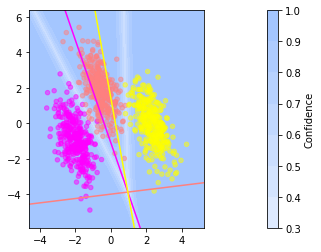
\includegraphics[width=3.8cm]{_static/softmax_regr_conf.png}
    };  
    \node[text width=3.5cm] at (5.5,-5) {transformation into a linearly classifiable space};
     \draw[blue]  (2.5,2) -- (3.5,2) -- (3.5,-2.6) -- (2.5,-2.6) -- (2.5,2);
    \draw[blue]  (0,-3) -- (7,-3) -- (7,-7) -- (0,-7) -- (0,-3);
    \draw[blue] (2.5,-2.6) -- (0,-3);
    \draw[blue] (3.5,-2.6) -- (7,-3); 
\end{tikzpicture}\end{center}

\section{Universal Approximation and the Representer Theorem}
\label{\detokenize{neuralnets_intro:universal-approximation-and-the-representer-theorem}}
\sphinxAtStartPar
The \sphinxstylestrong{Universal Approximation Theorem} states that a neural network with one hidden layer and enough hidden units can approximate any continuous function on a compact domain to arbitrary accuracy.

\sphinxAtStartPar
This power comes from \sphinxstylestrong{nonlinearity and compositional depth}.

\sphinxAtStartPar
In contrast, the \sphinxstylestrong{Representer Theorem} applies in kernel methods and shows that solutions to certain regularized learning problems lie in the span of training data. While neural networks do not directly satisfy the conditions of the theorem, they similarly perform \sphinxstylestrong{implicit regularization} through stochastic gradient descent and architectural constraints, guiding them toward simple, generalizable functions.

\sphinxstepscope


\section{Architecture}
\label{\detokenize{neuralnets_architecture:architecture}}\label{\detokenize{neuralnets_architecture::doc}}
\sphinxAtStartPar
The artificial neuron unit is the building block of ANNs. Thus, let us precisely model its behavior. The output value \( \hat{y} \) of an arbitrary neuron with \( D \) inputs is computed as
\begin{equation}\label{equation:neuralnets_architecture:neuron_output1}
\begin{split}\begin{eqnarray}
\hat{y} &=& \phi(a) \nonumber \\
&=& \phi \left( \sum_{i=1}^{D} w_{i} x_{i} + b \right),
\end{eqnarray}\end{split}
\end{equation}
\sphinxAtStartPar
where \( x_{i} \) is the input value (or feature) from the \( i \)\sphinxhyphen{}th previous neuron, \( w_{i} \) is the weight associated with the \( i \)\sphinxhyphen{}th input, \( b \) is a bias term, \( \phi(\cdot) \) is a non\sphinxhyphen{}linear activation function and \( a = \sum_{i=1}^{D} w_{i} x_{i} + b  \) is the activation. Alternatively, let the vector \( {\bf x} = \begin{bmatrix} x_{1} & \ldots & x_{D} \end{bmatrix}^{T} \) collect the input values from the \( D \) previous neurons and let \( {\bf w} = \begin{bmatrix} w_{1} & \ldots & w_{D} \end{bmatrix}^{T} \) collect the corresponding weights. We can write then the output value as
\begin{equation}\label{equation:neuralnets_architecture:neuron_output2}
\begin{split}\begin{equation}
\hat{y} = \phi \left( {\bf w}^{T} {\bf x} + b \right).
\end{equation}\end{split}
\end{equation}
\sphinxAtStartPar
Note therefore that \( {\bf w}^{T} {\bf x} + b = 0 \) defines a hyperplane over the \(D\)\sphinxhyphen{}dimensional input space. For convenience, we can further rewrite \eqref{equation:neuralnets_architecture:neuron_output1} by making the bias term implicit. More precisely, we absorb the bias into the weights by making \( w_{0} = b \) and create a new dummy input \( x_{0} = 1 \). Thus, we can write
\begin{equation}\label{equation:neuralnets_architecture:neuron_output3}
\begin{split}\begin{equation}
\hat{y} = \phi \left( \sum_{i=0}^{D} w_{i} x_{i} \right).
\end{equation}\end{split}
\end{equation}
\sphinxAtStartPar
More compactly, we can rewrite \eqref{equation:neuralnets_architecture:neuron_output3} in vector notation as
\begin{equation}\label{equation:neuralnets_architecture:neuron_output4}
\begin{split}\begin{equation}
\hat{y} = \phi \left( {\bf w}^{T} {\bf x} \right),
\end{equation}\end{split}
\end{equation}
\sphinxAtStartPar
where the vectors were redefined such that \( {\bf x} = \begin{bmatrix} x_{0} & x_{1} & \ldots & x_{D} \end{bmatrix}^{T} \) and \( {\bf w} = \begin{bmatrix} w_{0} & w_{1} & \ldots & w_{D} \end{bmatrix}^{T} \). That is, the output value \( \hat{y} \) is an affine function \( {\bf w}^{T} {\bf x} \) of the inputs in \( {\bf x} \) (activation) followed by a non\sphinxhyphen{}linearity \( \phi(\cdot) \) (activation function).

\sphinxAtStartPar
\hyperref[\detokenize{neuralnets_architecture:computational-graph1a}]{Fig.\@ \ref{\detokenize{neuralnets_architecture:computational-graph1a}}} illustrates the neuron unit computation steps graphically.


\begin{wrapfigure}{l}{0pt}
\centering
\noindent\sphinxincludegraphics[height=480\sphinxpxdimen]{{neuron_unit_computation_steps}.png}
\caption{Computation steps of a neuron.}\label{\detokenize{neuralnets_architecture:computational-graph1a}}\end{wrapfigure}

\sphinxAtStartPar
\hyperref[\detokenize{neuralnets_architecture:computational-graph1b}]{Fig.\@ \ref{\detokenize{neuralnets_architecture:computational-graph1b}}} shows the graphical representation of a single neuron unit. Note that the computational graph of a single neuron in \hyperref[\detokenize{neuralnets_architecture:computational-graph1b}]{Fig.\@ \ref{\detokenize{neuralnets_architecture:computational-graph1b}}} omits the summation in \hyperref[\detokenize{neuralnets_architecture:computational-graph1a}]{Fig.\@ \ref{\detokenize{neuralnets_architecture:computational-graph1a}}} required to compute the activation \(a\). Thus, we assume that the inward weighted input signals in \hyperref[\detokenize{neuralnets_architecture:computational-graph1b}]{Fig.\@ \ref{\detokenize{neuralnets_architecture:computational-graph1b}}} are all added up before applying the non\sphinxhyphen{}linearity \( \phi(\cdot) \).


\begin{wrapfigure}{l}{0pt}
\centering
\noindent\sphinxincludegraphics[height=480\sphinxpxdimen]{{neuron_unit_computational_graph}.png}
\caption{Computational graph of a neuron.}\label{\detokenize{neuralnets_architecture:computational-graph1b}}\end{wrapfigure}

\sphinxAtStartPar
An ANN is simply a computational graph comprising multiple artificial neurons (see \hyperref[\detokenize{neuralnets_architecture:computational-graph2}]{Fig.\@ \ref{\detokenize{neuralnets_architecture:computational-graph2}}}). Furthermore, the network topology is designed – one can play for example with the number hidden layers, number of units per layer and number of connections per unit – according to the specific task the network must perform e.g. indicate the class of objects on images. The task in turn is mapped into some arbitrarily complex function of the network inputs. Learning in this case consists in adjusting the network parameters (weights) such that the entire network approximates as good as possible the task function.


\begin{wrapfigure}{l}{0pt}
\centering
\noindent\sphinxincludegraphics[height=320\sphinxpxdimen]{{example_toy_ANN}.png}
\caption{Computational graph representing a toy neuron network comprising four neuron units. The illustrated network computes a function \( f: \mathbb{R}^{D} \rightarrow \mathbb{R} \) of its inputs (features) collected by the vector \( {\bf x} \). Note that \( f(\cdot) \) is an approximation to some task\sphinxhyphen{}related function that must be learned from data.}\label{\detokenize{neuralnets_architecture:computational-graph2}}\end{wrapfigure}

\sphinxAtStartPar
\hyperref[\detokenize{neuralnets_architecture:computational-graph3}]{Fig.\@ \ref{\detokenize{neuralnets_architecture:computational-graph3}}} shows the computational graph of a single hidden layer neural network with an \sphinxstyleemphasis{input} layer with \(D\) input units storing observed features \( \lbrace x_{i} \rbrace \), a \sphinxstyleemphasis{hidden} layer with \( H \) non\sphinxhyphen{}linear units (symbol \( \phi \)) computing \sphinxstyleemphasis{unobserved} (or embedded) features \( \lbrace h_{j} \rbrace \) and an \sphinxstyleemphasis{output} layer with a single linear unit (symbol \( \sum \)) yielding the network output \( \hat{y} = f({\bf x}) \).


\begin{wrapfigure}{l}{0pt}
\centering
\noindent\sphinxincludegraphics[height=320\sphinxpxdimen]{{single_layer_MLP}.png}
\caption{Computational graph representing a single hidden layer neural network. Weights were omitted in the graph for the sake of clarity.}\label{\detokenize{neuralnets_architecture:computational-graph3}}\end{wrapfigure}

\sphinxAtStartPar
The \(j\)\sphinxhyphen{}th hidden unit computes the \sphinxstyleemphasis{unobserved} feature as
\label{equation:neuralnets_architecture:e01fe95a-3f1f-4a02-88e0-b469822c510e}\begin{equation}
h_{j} = \phi \left( \sum_{i} w^{1}_{i,j} x_{i} \right). \nonumber
\end{equation}
\sphinxAtStartPar
Note that the superscript \( 1 \) indicates that the weight \( w^{1}_{i,j} \) belongs to an unit at the \sphinxstyleemphasis{first} (hidden) layer. On the other hand, the subscripts \( i,j \) indicates that the weight \( w^{1}_{i,j} \) corresponds to a synaptic connection between the \(i\)\sphinxhyphen{}th input unit and the \(j\)\sphinxhyphen{}th hidden unit. Lastly, the single output unit computes the network output as \begin{equation*}
\begin{split} \hat{y} = \sum_{j} w^{2}_{j,1} h_j, \end{split}
\end{equation*} where the superscript \( 2 \) indicates that the weight \( w^{2}_{j,1} \) belongs to the single unit \( 1 \) at the \sphinxstyleemphasis{second} (output) layer.

\sphinxAtStartPar
Alternatively, let the vectors \( {\bf x} = \begin{bmatrix} x_{0} = 1 & x_{1} & \ldots & x_{D} \end{bmatrix}^{T} \) and \( {\bf w}_{j}^{1} = \begin{bmatrix} w^{1}_{0,j} & w^{1}_{1,j} & \ldots & w^{1}_{D,j} \end{bmatrix}^{T} \) collect respectively the observed features and the corresponding weights at the \(j\)\sphinxhyphen{}th unit of the single hidden layer \( 1 \). The \(j\)\sphinxhyphen{}th \sphinxstyleemphasis{unobserved} (or embedded) feature can be rewritten then as
\label{equation:neuralnets_architecture:fac08fe0-de3a-4131-ae49-1dadeadca67f}\begin{equation}
h_{j} = \phi \left( ({\bf w}_{j}^{1})^{T} {\bf x} \right). \nonumber
\end{equation}
\sphinxAtStartPar
Analogously, let \( {\bf h} = \begin{bmatrix} h_{1} & h_{2} & \ldots & h_{H} \end{bmatrix}^{T} \) collect the embedded features and let \( {\bf w}_{1}^{2} = \begin{bmatrix} w^{2}_{1,1} & w^{2}_{2,1} & \ldots & w^{2}_{H,1} \end{bmatrix}^{T} \) collect the corresponding weights at the single unit of the output layer \( 2 \), we can rewrite the network output as
\label{equation:neuralnets_architecture:fd5fec0e-031f-4ce4-8bc4-60dc469551d0}\begin{equation}
\hat{y} = ({\bf w}_{1}^{2})^{T} {\bf h}. \nonumber
\end{equation}
\sphinxAtStartPar
Now, let the matrices
\label{equation:neuralnets_architecture:09b30da5-339f-4f49-a552-c618a11cf268}\begin{eqnarray}
{\bf W}^{1} &=& \begin{bmatrix} {\bf w}_{1}^{1} & \ldots & {\bf w}_{H}^{1} \end{bmatrix} \nonumber \\
&=& \begin{bmatrix} 
w^{1}_{0,1} & \ldots & w^{1}_{0,H} \\
w^{1}_{1,1} & \ldots & w^{1}_{1,H} \\
\vdots &  & \vdots \\
w^{1}_{D,1} & \ldots & w^{1}_{D,H} \nonumber
\end{bmatrix}
\end{eqnarray}
\sphinxAtStartPar
and
\label{equation:neuralnets_architecture:c3dda1b2-fb3e-49be-b330-46d5e5b81d0d}\begin{eqnarray}
{\bf W}^{2} &=& \begin{bmatrix} {\bf w}_{1}^{2} \end{bmatrix} \nonumber \\
&=& \begin{bmatrix} 
w^{2}_{1,1} \\
\vdots \\
w^{2}_{H,1} \nonumber
\end{bmatrix}
\end{eqnarray}
\sphinxAtStartPar
collect all weights at layers \( 1 \) and \( 2 \), respectively, such that the \(j\)\sphinxhyphen{}th column stores the weights \( \lbrace w^{\ell}_{\bullet,j} \rbrace \) of the \(j\)\sphinxhyphen{}th unit at the corresponding layer \( \ell \). We can further rewrite the network output in compact vector\sphinxhyphen{}matrix notation as
\label{equation:neuralnets_architecture:067f614f-2bdb-4471-9f14-3e434aee03be}\begin{eqnarray}
\hat{y} &=& ({\bf W}^{2})^{T} {\bf h} \nonumber \\
&=& ({\bf W}^{2})^{T} \phi \left( {\bf a} \right) \nonumber \\
&=& ({\bf W}^{2})^{T} \phi \left( ({\bf W}^{1})^{T} {\bf x} \right), \nonumber
\end{eqnarray}
\sphinxAtStartPar
in which the non\sphinxhyphen{}linearity is applied element\sphinxhyphen{}wise along the activation vector \( {\bf a} = \begin{bmatrix} a_{1} & a_{2} & \ldots & a_{H} \end{bmatrix}^{T} \) such that \( h_{j} = \phi(a_{j}) \), \( \forall j \in \lbrace 1, \ldots, H \rbrace \). Therefore, the output of the single hidden layer network in \hyperref[\detokenize{neuralnets_architecture:computational-graph3}]{Fig.\@ \ref{\detokenize{neuralnets_architecture:computational-graph3}}} is equivalent to applying an affine transformation \( ({\bf W}^{1})^{T} {\bf x} \) to the network inputs \( {\bf x} \) followed by a non\sphinxhyphen{}linearity \( \phi \) to obtain the embedded features \( {\bf h} \) followed by a new affine transformation \( ({\bf W}^{2})^{T} {\bf h} \) to obtain the final output \( \hat{y} \).

\begin{sphinxadmonition}{attention}{Attention:}
\sphinxAtStartPar
The network capacity is determined by the number of network parameters (weights). As we increase the network capacity, we increase the network flexibility to fit the training examples. Going too far increasing the capacity and the network will overfit the training examples. On the other hand, the network will underfit the training examples with a too small capacity. In both cases, the network loses its ability to properly generalize, i.e. to provide a good approximation of the task\sphinxhyphen{}related function for unseen input patterns \( {\bf x} \) belonging, for instance, to a testing dataset.
\end{sphinxadmonition}


\section{Neural Networks: Architecture and Building Blocks}
\label{\detokenize{neuralnets_architecture:neural-networks-architecture-and-building-blocks}}
\sphinxAtStartPar
Neural networks stack multiple linear models interleaved with \sphinxstylestrong{nonlinear activation functions} to create deep, hierarchical representations.


\subsection{4.1 Linear Layers and Activations}
\label{\detokenize{neuralnets_architecture:linear-layers-and-activations}}
\sphinxAtStartPar
The most basic neural network layer performs a linear transformation:
\begin{equation*}
\begin{split}
\mathbf{z} = \mathbf{W}\mathbf{x} + \mathbf{b}
\end{split}
\end{equation*}
\sphinxAtStartPar
This is followed by a \sphinxstylestrong{nonlinear activation function} \( \phi \), such as:
\begin{itemize}
\item {} 
\sphinxAtStartPar
ReLU: \( \phi(z) = \max(0, z) \)

\item {} 
\sphinxAtStartPar
Sigmoid: \( \phi(z) = \frac{1}{1 + e^{-z}} \)

\item {} 
\sphinxAtStartPar
Tanh: \( \phi(z) = \frac{e^z - e^{-z}}{e^z + e^{-z}} \)

\end{itemize}

\sphinxAtStartPar
A simple feedforward neural network (MLP) with one hidden layer:
\begin{equation*}
\begin{split}
\begin{align*}
\mathbf{h} &= \phi(\mathbf{W}_1 \mathbf{x} + \mathbf{b}_1) \\
\hat{\mathbf{y}} &= \text{softmax}(\mathbf{W}_2 \mathbf{h} + \mathbf{b}_2)
\end{align*}
\end{split}
\end{equation*}
\sphinxAtStartPar
Each layer composes the previous one, enabling complex function approximation.


\section{Convolutional Neural Networks (CNNs)}
\label{\detokenize{neuralnets_architecture:convolutional-neural-networks-cnns}}
\sphinxAtStartPar
For high\sphinxhyphen{}dimensional data like images, \sphinxstylestrong{convolutional layers} exploit local spatial structure:
\begin{equation*}
\begin{split}
\text{Conv}(\mathbf{x}) = \sum_{i,j} \mathbf{K}_{i,j} \cdot \mathbf{x}_{i:i+k, j:j+k}
\end{split}
\end{equation*}
\sphinxAtStartPar
CNNs use:
\begin{itemize}
\item {} 
\sphinxAtStartPar
\sphinxstylestrong{Local connectivity} (kernels are small spatial patches)

\item {} 
\sphinxAtStartPar
\sphinxstylestrong{Weight sharing} (same kernel applied across the image)

\item {} 
\sphinxAtStartPar
\sphinxstylestrong{Pooling} to reduce dimensionality

\end{itemize}

\sphinxAtStartPar
These principles allow CNNs to be efficient and translationally invariant.


\section{Skip Connections and Deep Architectures}
\label{\detokenize{neuralnets_architecture:skip-connections-and-deep-architectures}}
\sphinxAtStartPar
Deeper networks can suffer from \sphinxstylestrong{vanishing gradients} or degraded performance. \sphinxstylestrong{Skip connections} (or residual connections) address this by allowing the gradient to flow more directly:
\begin{equation*}
\begin{split}
\mathbf{h}_{l+1} = \phi(\mathbf{W}_l \mathbf{h}_l + \mathbf{b}_l) + \mathbf{h}_l
\end{split}
\end{equation*}
\sphinxAtStartPar
This enables \sphinxstylestrong{ResNets} and other deep architectures to train effectively, and has become a standard design choice in modern networks.

\sphinxstepscope


\section{Function approximator}
\label{\detokenize{neuralnets_func_approx:function-approximator}}\label{\detokenize{neuralnets_func_approx::doc}}
\sphinxAtStartPar
What do we mean exactly by a \sphinxstyleemphasis{complex task}? ANNs build high\sphinxhyphen{}dimensional complex functions using simple modules – artificial neurons. However, like the brain, ANNs are black boxes and are hard to interpret, i.e. to clearly understand how they get their final output. Nevertheless, ANNs are universal approximators, they can approximate any function as indicated in the following theorem shown by Pinkus {[}\hyperlink{cite.bibliography:id17}{5}{]}.
\label{neuralnets_func_approx:approximator}
\begin{sphinxadmonition}{note}{Theorem 27 (Pinkus Theorem)}



\sphinxAtStartPar
Any continuous function \(f^{\ast} \colon \mathbb{R}^{D} \rightarrow \mathbb{R}^{O}\) can be arbitrarily well approximated (on any compact set) by a single layer neural network, for a wide range of non\sphinxhyphen{}linearities \(\phi\) (non\sphinxhyphen{}polynomials).
\end{sphinxadmonition}


\begin{wrapfigure}{l}{0pt}
\centering
\noindent\sphinxincludegraphics[height=320\sphinxpxdimen]{{images/neuralnets/network_approximation}.svg}
\caption{Network approximation \( f \colon \mathbb{R}^{D} \rightarrow \mathbb{R}^{O} \) to a continuous function \( f^{\ast} \colon \mathbb{R}^{D} \rightarrow \mathbb{R}^{O} \). For a given observed feature vector \( \check{\bf x} \in \mathbb{R}^{D} \), the network estimates the output as \( \hat{\bf y} = f(\check{\bf x}) \in \mathbb{R}^{O} \) as opposed to the true output \( {\bf y} = f^{\ast}(\check{\bf x}) \in \mathbb{R}^{O} \) that would be obtained by the approximated function \( f^{\ast} \). Lastly, note that the network task represented by the function \(f^{\ast}\) can be arbitrarily complex e.g. convert speech\sphinxhyphen{}to\sphinxhyphen{}text.}\label{\detokenize{neuralnets_func_approx:network-approximation}}\end{wrapfigure}

\sphinxAtStartPar
Note that we need to employ a non\sphinxhyphen{}linear activation function \(\phi \colon \mathbb{R} \rightarrow \mathbb{R} \). \hyperref[\detokenize{neuralnets_func_approx:activation-functions}]{Fig.\@ \ref{\detokenize{neuralnets_func_approx:activation-functions}}} illustrates some widespread activation functions in machine learning literature. Common activation functions in traditional machine learning are the sigmoid
\label{equation:neuralnets_func_approx:75248184-94a3-4def-b69b-a02c1a966be9}\begin{equation}
\phi(x) = \frac{1}{1+e^{-x}}
\end{equation}
\sphinxAtStartPar
and hyperbolic tangent
\label{equation:neuralnets_func_approx:f00c718e-5eb6-4b43-b7ce-c70a2e9519d3}\begin{equation}
\phi(x) = \frac{e^{x}-e^{-x}}{e^{x}+e^{-x}}.
\end{equation}
\sphinxAtStartPar
However, modern deep learning methods typically use unbounded, non\sphinxhyphen{}linear activation functions such as the rectified linear unit (ReLU)
\label{equation:neuralnets_func_approx:6d7fc53c-5b8f-41e2-9915-9082940be875}\begin{equation}
\phi(x) = \max(0, x),
\end{equation}
\sphinxAtStartPar
the leaky ReLU
\label{equation:neuralnets_func_approx:9d9a6c56-5123-4b2f-96c7-9914565af7b5}\begin{equation}
\phi(x) = \max(\alpha x, x)
\end{equation}
\sphinxAtStartPar
or the exponential linear unit (LU)
\label{equation:neuralnets_func_approx:e8239ac6-6721-40bf-858e-96dcde4e286f}\begin{equation}
\phi(x) = \left\lbrace 
\begin{matrix}
x, & x \geq 0 \\
\alpha \left( e^{x}-1 \right), & \mbox{otherwise}
\end{matrix}
\right.
\end{equation}
\sphinxAtStartPar
in which \( \alpha \geq 0 \) is a small constant e.g. \( \alpha = 0.1 \).

\sphinxAtStartPar
Activation functions are carefully designed such that their derivatives are available in closed form and can be computed very efficiently. For example, for the sigmoid and ReLU activation functions, the derivatives are straightforwardly computed respectively as
\label{equation:neuralnets_func_approx:ec8bd5b2-4409-42f0-a8d9-363f52084e8d}\begin{equation}
\phi'(x) =  \frac{\partial \phi(x)}{\partial x} =  \phi(x) \, \phi(-x)
\end{equation}
\sphinxAtStartPar
and
\label{equation:neuralnets_func_approx:49ca0e92-c4d0-44bd-92ad-0fd115fea0e9}\begin{equation}
\phi'(x) =  \frac{\partial \phi(x)}{\partial x} =  \left[ x \geq 0 \right],
\end{equation}
\sphinxAtStartPar
where the Iverson bracket \( \left[ \Psi \right] \) yields \( 1 \) if the logical proposition \( \Psi \) is true or \( 0 \), otherwise.


\begin{wrapfigure}{l}{0pt}
\centering
\noindent\sphinxincludegraphics[height=480\sphinxpxdimen]{{activation_functions}.png}
\caption{Common non\sphinxhyphen{}linear activation functions (borrowed from {[}\hyperlink{cite.bibliography:id18}{7}{]}). In contrast to traditional ones, modern activation functions are typically unbounded and can be computed very efficiently.}\label{\detokenize{neuralnets_func_approx:activation-functions}}\end{wrapfigure}

\begin{sphinxadmonition}{important}{Important:}
\sphinxAtStartPar
Modern activation functions are unbounded such that their output values do not saturate and their derivatives do not collapse to zero for larger activation values (see \hyperref[\detokenize{neuralnets_func_approx:sigmoid-function}]{Fig.\@ \ref{\detokenize{neuralnets_func_approx:sigmoid-function}}} and \hyperref[\detokenize{neuralnets_func_approx:relu-function}]{Fig.\@ \ref{\detokenize{neuralnets_func_approx:relu-function}}}). This is paramount in deep neural networks, since the activation values might become bigger and bigger as the feed input features \( \lbrace x_{i} \rbrace \) are forwarded over the network. Moreover, unbounded activation functions – with non\sphinxhyphen{}zero derivatives – are crucial for the deep learning itself. As we will see shortly (in the backpropagation procedure), the network weights are updated in order to minimize some loss function \( L(y,\hat{y}) \). Specifically, each weight is updated using the back propagated derivatives of the loss function in respect to the weight itself. To accomplish this, the chain rule of calculus is applied several times over potentially long branches of the associated computational graph linking the parameter to the network outputs. Additionally, the product of chained derivatives might become smaller and smaller as derivatives are back propagated through the network. Note though that, when the activation function saturates, its derivative becomes close to zero. Thus, if that happens in all paths between a network parameter and the network outputs, this parameter will become insensitive to the improvements in the loss function and will not be updated anymore, i.e. the network will not learn to perform its task based on this parameter.

\sphinxAtStartPar
\hyperref[\detokenize{neuralnets_func_approx:sigmoid-function}]{Fig.\@ \ref{\detokenize{neuralnets_func_approx:sigmoid-function}}} and \hyperref[\detokenize{neuralnets_func_approx:relu-function}]{Fig.\@ \ref{\detokenize{neuralnets_func_approx:relu-function}}} show respectively the sigmoid and ReLU activation functions and their derivatives.


\begin{wrapfigure}{l}{0pt}
\centering
\noindent\sphinxincludegraphics[height=320\sphinxpxdimen]{{sigmoid_d}.png}
\caption{Sigmoid activation function. The sigmoid derivative collapses to zero for large absolute values of the activation.}\label{\detokenize{neuralnets_func_approx:sigmoid-function}}\end{wrapfigure}


\begin{wrapfigure}{l}{0pt}
\centering
\noindent\sphinxincludegraphics[height=320\sphinxpxdimen]{{relu_d}.png}
\caption{ReLU activation function. The ReLU function derivative remains constant for large positive activation values.}\label{\detokenize{neuralnets_func_approx:relu-function}}\end{wrapfigure}
\end{sphinxadmonition}
\label{neuralnets_func_approx:example-1}
\begin{sphinxadmonition}{note}{Example 21}



\sphinxAtStartPar
Suppose a linear activation function of the type \( \phi(a) = \kappa a \). It can be shown that the resulting network can be actually reduced to a single linear neuron unit with properly adjusted weights \( \tilde{\bf w} = \begin{bmatrix} \tilde{w}_{0} \equiv \tilde{b} & \tilde{w}_{1} & \ldots & \tilde{w}_{D} \end{bmatrix} \), i.e. the network will not be able to approximate any function more complex than an affine transform \( \hat{y} = f({\bf x}) = \tilde{\bf w}^{T} {\bf x} \) of its inputs \( {\bf x} = \begin{bmatrix} {x}_{0} \equiv 1 & {x}_{1} & \ldots & {x}_{D} \end{bmatrix} \). Thus, a non\sphinxhyphen{}linear activation function is required for the network to approximate more complex functions.

\sphinxAtStartPar
\hyperref[\detokenize{neuralnets_func_approx:computational-graph4}]{Fig.\@ \ref{\detokenize{neuralnets_func_approx:computational-graph4}}} shows an example of a linear network with activation function \( \phi(a) = a \).


\begin{wrapfigure}{l}{0pt}
\centering
\noindent\sphinxincludegraphics[height=320\sphinxpxdimen]{{example_ANN_linear_02}.png}
\caption{The need for non\sphinxhyphen{}linearity. Computational graph comprising three linear neuron units on the left is equivalently to a single linear unit on the right.}\label{\detokenize{neuralnets_func_approx:computational-graph4}}\end{wrapfigure}

\sphinxAtStartPar
Note that in this case we have
\label{equation:neuralnets_func_approx:36d0f0ff-fa8f-4724-ba0b-249b875fc216}\begin{eqnarray}
\hat{y} &=& w_{0,1}^{2} + \sum_{j=1}^2 w^{2}_{j,1} \left( \sum_{i=0}^D w^{1}_{i,j} x_{i} \right) \nonumber \\
&=& \sum_{i=0}^D \tilde{w}_{i} x_{i}. \nonumber
\end{eqnarray}
\sphinxAtStartPar
Thus, the network is equivalent to a single unit with weights \begin{equation*}
\begin{split} \tilde{w}_{0} = {w^{2}_{0,1}} + w^{1}_{0,1} \, w^{2}_{1,1} +  w^{1}_{0,2} \, w^{2}_{2,1} \end{split}
\end{equation*} and \begin{equation*}
\begin{split} \tilde{w}_{i} = w^{1}_{i,1} \, w^{2}_{1,1} +  w^{1}_{i,2} \, w^{2}_{2,1}, \,\,\, \forall i \in \lbrace 1, \ldots, D \rbrace. \end{split}
\end{equation*}
\end{sphinxadmonition}

\sphinxstepscope


\section{Multi\sphinxhyphen{}Layer Perceptrons}
\label{\detokenize{neuralnets_mlps:multi-layer-perceptrons}}\label{\detokenize{neuralnets_mlps::doc}}
\sphinxAtStartPar
Multi\sphinxhyphen{}Layer Perceptrons (MLPs) a.k.a. Multi\sphinxhyphen{}Layer Feed\sphinxhyphen{}Forward Neural Networks are obtained by stacking multiple hidden layers. Each hidden layer can contain different number of hidden units. In general, a MLP has \(L\) hidden layers with \(H_{1}, H_{2}, \ldots, H_{L} \) hidden units, i.e. the \(\ell\)\sphinxhyphen{}th hidden layer contains \(H_{\ell}\) hidden units. For convenience, we also assume that the network inputs correspond to a layer \( 0 \) with \( H_{0} = D \) units. Lastly, the \( L\)\sphinxhyphen{}th layer can directly produce the network outputs. In this case, \( H_{L} = O \). Alternatively, the \( H_{L} \) values at the last layer can be combined \sphinxstyleemphasis{somehow} to produce the final network estimate \( \hat{\bf y} = f({\bf x}) \). In this case, \( H_{L} \) is not necessarily equal to \( O \).

\sphinxAtStartPar
The figures below illustrate MLPs with different number of hidden layers. \hyperref[\detokenize{neuralnets_mlps:mlp1-fig1}]{Fig.\@ \ref{\detokenize{neuralnets_mlps:mlp1-fig1}}} shows a MLP network with a single hidden layer, \hyperref[\detokenize{neuralnets_mlps:mlp1-fig2}]{Fig.\@ \ref{\detokenize{neuralnets_mlps:mlp1-fig2}}} a MLP with two hidden layers and \hyperref[\detokenize{neuralnets_mlps:mlp1-fig3}]{Fig.\@ \ref{\detokenize{neuralnets_mlps:mlp1-fig3}}} a MLP with tree hidden layers. Note that each layer \(\ell\) can use a distinct activation function \(\phi_{\ell}\). Note that the values from the last hidden layer units are being combined by means of a single linear unit – affine transform represented by the symbol \( \sum \) – to produce the final network estimate \( \hat{y} = f({\bf x}) \) (\( O = 1 \)). However, as we will see later, other ways to combine are also possible.


\begin{wrapfigure}{l}{0pt}
\centering
\noindent\sphinxincludegraphics[height=320\sphinxpxdimen]{{multi_layer_MLP_01}.png}
\caption{1\sphinxhyphen{}layer MLP (\(L=1\)).}\label{\detokenize{neuralnets_mlps:mlp1-fig1}}\end{wrapfigure}


\begin{wrapfigure}{l}{0pt}
\centering
\noindent\sphinxincludegraphics[height=320\sphinxpxdimen]{{multi_layer_MLP_05}.png}
\caption{2\sphinxhyphen{}layer MLP (\(L=2\))}\label{\detokenize{neuralnets_mlps:mlp1-fig2}}\end{wrapfigure}


\begin{wrapfigure}{l}{0pt}
\centering
\noindent\sphinxincludegraphics[height=320\sphinxpxdimen]{{multi_layer_MLP_07}.png}
\caption{3\sphinxhyphen{}layer MLP (\(L=3\)).}\label{\detokenize{neuralnets_mlps:mlp1-fig3}}\end{wrapfigure}

\sphinxAtStartPar
Let \( w^{\ell}_{i,j} \) denote the artificial synaptic weight from the \(i\)\sphinxhyphen{}th unit in previous layer \( \ell-1 \) to the \(j\)\sphinxhyphen{}th unit in the current layer \( \ell\) and let vector \( {\bf w}^{\ell}_{j} = \begin{bmatrix} w^{\ell}_{0,j} & w^{\ell}_{1,j} & \ldots & w^{\ell}_{H_{\ell-1},j} \end{bmatrix}^{T}\) collect all weights of the \(j\)\sphinxhyphen{}th unit at layer \(\ell\). Additionally, for convenience, let \( {\bf h}^{0} = \begin{bmatrix} 1 & x_{1} & x_{2} & \ldots & x_{D} \end{bmatrix}^{T} \) with \( H_{0} = D \) collect the observed features and let \( {\bf h}^{\ell} = \begin{bmatrix} 1 & h^{\ell}_{1} & h^{\ell}_{2} & \ldots & h^{\ell}_{H_{\ell}} \end{bmatrix}^{T} \) collect the embedded features for all \( \ell \in \lbrace 1, \ldots, L \rbrace \). Thus, we can write the activation value of the \(j\)\sphinxhyphen{}th unit of the current layer \( \ell \) using vector notation as
\label{equation:neuralnets_mlps:b74f1438-1634-4ad9-a322-05d5471b9740}\begin{eqnarray}
a^{\ell}_{j} &=& \sum_{i=0}^{H_{\ell-1}} w^{\ell}_{i,j} \, h^{\ell-1}_{i} \nonumber \\
&=& ({\bf w}_{j}^{\ell})^{T} {\bf h}^{\ell-1}. \nonumber
\end{eqnarray}
\sphinxAtStartPar
Finally, the output value of this neuron is computed as \begin{equation*}
\begin{split} h^{\ell}_{j} = \phi_{\ell}\left( a^{\ell}_{j} \right). \end{split}
\end{equation*}

\sphinxAtStartPar
Now, let the matrix \( {\bf W}^{\ell} = \left[  w^{\ell}_{i,j} \right] \) collect the weights of all units at the \(\ell\)\sphinxhyphen{}th layer such that its \(j\)\sphinxhyphen{}th column stores the weights associated with the \(j\)\sphinxhyphen{}th unit at layer \(\ell\). Equivalently, we can write \( {\bf W}^{\ell} = \begin{bmatrix} {\bf w}^{\ell}_{1} & {\bf w}^{\ell}_{2} & \ldots & {\bf w}^{\ell}_{H_{\ell}} \end{bmatrix} \). Furthermore, let the vector \( {\bf a}^{\ell} = \begin{bmatrix} a^{\ell}_{1} & a^{\ell}_{2} & \ldots & a^{\ell}_{H_{\ell}} \end{bmatrix}^{T} \) collect all activations \(a^{\ell}_{j}\) of layer \(\ell\). Then, we can conveniently write \({\bf a}^{\ell}\) and \( {\bf h}^{\ell} \) as matrix\sphinxhyphen{}vector products
\label{equation:neuralnets_mlps:22491dbb-ef41-4fff-96ce-9ccea677d58f}\begin{eqnarray}
{\bf a}^{\ell} &=& ({\bf W}^{\ell})^{T} \, {\bf h}^{\ell-1} \nonumber \\
{\bf h}^{\ell} &=& \phi_{\ell}({\bf a}^{\ell}), \nonumber
\end{eqnarray}
\sphinxAtStartPar
in which the non\sphinxhyphen{}linearity \( \phi_{\ell} \) is applied element\sphinxhyphen{}wise on the vector \( {\bf a}^{\ell} \).

\sphinxAtStartPar
Therefore, the \(\ell\)\sphinxhyphen{}th layer output can be computed from the output of the previous layer \( \ell -1 \) as
\begin{equation}\label{equation:neuralnets_mlps:mlp_recursion}
\begin{split}\begin{eqnarray}
{\bf h}^{\ell} &=& \phi_{\ell} \left( ({\bf W}^{\ell})^{T} \, {\bf h}^{\ell-1} \right)
\end{eqnarray}\end{split}
\end{equation}
\sphinxAtStartPar
and the last layer output can be computed by recursively applying \eqref{equation:neuralnets_mlps:mlp_recursion} starting with \( {\bf h}^{0} \) – vector storing the network inputs in \( {\bf x} \) – until obtain \( {\bf h}^{L} \) – vector collecting the values produced by the units at the last layer. Finally, the last layer output can be further \sphinxstyleemphasis{combined} to produce the network output \( \hat{\bf y} = f({\bf x}) \).

\sphinxAtStartPar
The computation performed by the 3\sphinxhyphen{}layer network illustrated in \hyperref[\detokenize{neuralnets_mlps:mlp1-fig3}]{Fig.\@ \ref{\detokenize{neuralnets_mlps:mlp1-fig3}}} can be written using a single line as \begin{equation*}
\begin{split} f({\bf x}) = \underbrace{({\bf W}^{4})^{T}
\phi_3 \Big(
\underbrace{({\bf W}^{3})^{T} \phi_2 \Big(
\underbrace{({\bf W}^{2})^{T} 
\phi_1 \Big(
\underbrace{({\bf W}^{1})^{T} {\bf h}^{0}}_{\mathbf{a}^{1}} 
\Big)}_{\mathbf{a}^{2}} \Big)}_{\mathbf{a}^{3}} \Big)}_{\hat{y}} \end{split}
\end{equation*} in which \( \mathbf{W}^{4} \) is \(H_L \times O\) matrix and \( {\bf h}^{0} \triangleq \begin{bmatrix} 1 & {\bf x}^{T} \end{bmatrix}^{T} \) with \( {\bf x} = \begin{bmatrix} x_1 & x_2 & \ldots & x_D \end{bmatrix}^{T} \). In this example, the single linear output unit – node with symbol \( \sum \) in \hyperref[\detokenize{neuralnets_mlps:mlp1-fig3}]{Fig.\@ \ref{\detokenize{neuralnets_mlps:mlp1-fig3}}} – uses an affine transform (\( \mathbf{W}^{4} \)) to combine the \(H_L\) values at last hidden layer into a single output \( \hat{y} \), i.e. \(O=1\). For multiple outputs, we can design \( \mathbf{W}^{4} \) such that \(O > 1\). The MLP is thus a nested sequence of matrix\sphinxhyphen{}vector multiplications each of them followed by an element\sphinxhyphen{}wise non\sphinxhyphen{}linearity.
\label{neuralnets_mlps:definition-0}
\begin{sphinxadmonition}{note}{Definition 33 (Expressive Efficiency phenomenon)}



\sphinxAtStartPar
As stated by Pinkus {[}\hyperlink{cite.bibliography:id17}{5}{]} (see {\hyperref[\detokenize{neuralnets_func_approx::doc}]{\sphinxcrossref{\DUrole{doc}{Function approximator}}}} page), single layer neural networks can approximate arbitrarily well any continuous function \(f^{\ast} \colon \mathbb{R}^{D} \rightarrow \mathbb{R}^{O}\) for a wide range of non\sphinxhyphen{}linearities \(\phi\). Thus, why do we need multiple layers?

\sphinxAtStartPar
The motivation to use multiple layers is related to a phenomenon called \sphinxstyleemphasis{Expressive Efficiency}:
\begin{itemize}
\item {} 
\sphinxAtStartPar
Despite being universal approximators, shallow networks with a single hidden layer might require an exponential size – number of hidden layer units – on the number of inputs to approximate some function classes.

\item {} 
\sphinxAtStartPar
On the other hand, the number of neurons required by a deep network with several hidden layers to represent the same functions has polynomial growth on the number of network inputs.

\end{itemize}

\sphinxAtStartPar
Thus, deep networks can represent non\sphinxhyphen{}linear functions more efficiently than shallow ones. A classical example is the \sphinxstyleemphasis{parity function}, which requires exponential size in shallow networks, but polynomial size in deep networks.

\sphinxAtStartPar
The intuition behind the \sphinxstyleemphasis{Expressive Efficiency} phenomenon is as follows. Typical real\sphinxhyphen{}world tasks e.g. \sphinxstyleemphasis{predict apple/pear from an image} are associated with highly non\sphinxhyphen{}linear functions of the type \(f^{\ast} \colon \mathbb{R}^{D} \rightarrow \mathbb{R}^{O} \). However, common activation functions \(\phi \colon \mathbb{R} \rightarrow \mathbb{R} \) e.g. sigmoid and ReLU employed by the network units show simple non\sphinxhyphen{}linearities. A single layer (shallow) network therefore would required a prohibitive number of units to express these real\sphinxhyphen{}world non\sphinxhyphen{}linearities, i.e. to approximate \(f^{\ast} \). On the other hand, by cascading multiple non\sphinxhyphen{}linear layers, a deep network improves its ability / flexibility to express non\sphinxhyphen{}linearities and, therefore, is able to provide a reasonable approximation to \(f^{\ast} \) using fewer neurons.
\end{sphinxadmonition}

\sphinxstepscope


\section{Backpropagation}
\label{\detokenize{neuralnets_backprop:backpropagation}}\label{\detokenize{neuralnets_backprop::doc}}
\sphinxAtStartPar
Neural networks are powerful function approximators, with thousands, millions or even billions of parameters that must be tuned (learned). But how do they learn these parameters from data?

\sphinxAtStartPar
In short, we need first to define a loss function indicating what the network should learn. More precisely, the loss function must express how good (or bad) the network is performing the task it is supposed to do during training. Thus, the selection of the loss function often depends on the kind of task the network must perform. For example, we typically use:
\begin{itemize}
\item {} 
\sphinxAtStartPar
the mean squared error (MSE) for regression tasks; and

\item {} 
\sphinxAtStartPar
the cross entropy for classification tasks.

\end{itemize}

\sphinxAtStartPar
In the sequel, we must adjust the network parameters to reduce the training loss. This machine learning problem is commonly stated as an \sphinxstyleemphasis{optimization problem} and it is frequently solved by means of \sphinxstyleemphasis{gradient descent} methods. The backpropagation algorithm, in turn, provides a systematic procedure to compute gradients over the computational graph representing computations across an artificial neural network. Specifically, it employs the chain rule of calculus with a lot of \sphinxstyleemphasis{bookkeeping} to allow one to compute the gradient of the training loss w.r.t. each network parameter. Thus, backpropagation plays a major role to allow one to use gradient descent methods for learning the network parameters.

\sphinxAtStartPar
{\hyperref[\detokenize{neuralnets_backprop:learning_alg}]{\sphinxcrossref{Algorithm 11}}} summarizes this high\sphinxhyphen{}level learning procedure which employs the back propagation of the \sphinxstyleemphasis{prediction quality} – encoded in the loss function – to adjust the weights of the artificial synapses.
\label{neuralnets_backprop:learning_alg}
\begin{sphinxadmonition}{note}{Algorithm 11 (Learning procedure)}



\sphinxAtStartPar
\sphinxstylestrong{Inputs}
\begin{itemize}
\item {} 
\sphinxAtStartPar
Network structure and hyper\sphinxhyphen{}parameters.

\end{itemize}

\sphinxAtStartPar
\sphinxstylestrong{Output}
\begin{itemize}
\item {} 
\sphinxAtStartPar
Trained / tunned network parameters.

\end{itemize}

\sphinxAtStartPar
\sphinxstylestrong{Function} Learn network parameters
\begin{enumerate}
\sphinxsetlistlabels{\arabic}{enumi}{enumii}{}{.}%
\item {} 
\sphinxAtStartPar
Initialize network parameters

\item {} 
\sphinxAtStartPar
\sphinxstylestrong{repeat}
\begin{enumerate}
\sphinxsetlistlabels{\arabic}{enumii}{enumiii}{}{.}%
\item {} 
\sphinxAtStartPar
Compute the training loss, i.e. assess the network prediction quality.

\item {} 
\sphinxAtStartPar
Back propagate training loss gradients w.r.t. network parameters.

\item {} 
\sphinxAtStartPar
Change parameters a bit to reduce the loss. \sphinxstyleemphasis{(Gradient descent step)}

\end{enumerate}

\item {} 
\sphinxAtStartPar
\sphinxstylestrong{until} Reach some stop criteria

\item {} 
\sphinxAtStartPar
\sphinxstylestrong{return} Trained network parameters

\end{enumerate}
\end{sphinxadmonition}


\subsection{Loss functions}
\label{\detokenize{neuralnets_backprop:loss-functions}}
\sphinxAtStartPar
There are several loss functions we can use. For convenience, let \( {\bf w} \) be a long vector collecting all neural network parameters, i.e. the vector \( {\bf w} \) collect the parameters \( \mathbf{W}^{1}, \mathbf{W}^{2}, \ldots, \mathbf{W}^{L} \) from all network layers. Now, let \( \hat{y} = f({\bf x}; {\bf w}) \) be the network’s output for input vector \( {\bf x} \) and network parameters \( {\bf w} \). The loss function \(L(y, \hat{y})\) – a.k.a. risk or cost function – measures how well the prediction \(\hat{y}\) approximates the target \(y\). Moreover, the training loss, i.e. the empirical risk, is computed using the training samples \begin{equation*}
\begin{split} {\cal D}_{train} = \bigcup_{i=1}^{N} \lbrace \left( {\bf x}_{i}, y_{i} \right) \rbrace \end{split}
\end{equation*} as
\begin{equation}\label{equation:neuralnets_backprop:empirical_risk}
\begin{split}\begin{eqnarray}
L_{train} &=& \frac{1}{N} \sum_{i=1}^{N} L \left( y_{i}, \hat{y}_{i} \right) \\
&=& \frac{1}{N} \sum_{i=1}^{N} L \left( y_{i}, f({\bf x}_{i}; {\bf w}) \right).
\end{eqnarray}\end{split}
\end{equation}
\sphinxAtStartPar
As mentioned above, the most common loss for regression is the Mean Square Error (MSE). The squared error is defined as
\begin{equation}\label{equation:neuralnets_backprop:squared_error}
\begin{split}\begin{equation}
L(y, \hat{y}) = (\hat{y} - y)^2
\end{equation}\end{split}
\end{equation}
\sphinxAtStartPar
and its partial derivative w.r.t. estimate \( \hat{y} \) is given simple by
\label{equation:neuralnets_backprop:ec7c3c4c-dbbc-4dcd-9e21-8327e673f5cc}\begin{equation}
{\partial L(y, \hat{y}) \over \partial \hat{y}} = 2 (\hat{y} - y).
\end{equation}
\sphinxAtStartPar
The Mean Squared Error (MSE) in turn is obtained by plugging \eqref{equation:neuralnets_backprop:squared_error} into the empirical risk \eqref{equation:neuralnets_backprop:empirical_risk}
\label{equation:neuralnets_backprop:e778dfca-47c1-490e-8cd0-627dfa62b95a}\begin{eqnarray}
L_{train} &=& MSE(y, \hat{y}; {\bf w}) \\
&=& \frac{1}{N} \sum_{i=1}^{N} (\hat{y}_{i} - y_{i})^2  \\
 &=& \frac{1}{N} \sum_{i=1}^{N} (f({\bf x}_{i}; {\bf w}) - y_{i})^2.
\end{eqnarray}
\sphinxAtStartPar
On the other hand, a Cross Entropy (CE) loss function is frequently employed for classification tasks. But how do we setup a neural network as a classifier? Let \(C\) denote the number of classes among the network must decide. First, we employ \(C\) linear units at the last hidden layer of the network, i.e. the vector \( {\bf h}^{L} \) collecting the outputs of the last hidden layer has \( C \) elements. Then, we use a \sphinxstyleemphasis{softmax} activation to convert this vector into a probability distribution.

\sphinxAtStartPar
In the example of \hyperref[\detokenize{neuralnets_backprop:classification-mlp-fig}]{Fig.\@ \ref{\detokenize{neuralnets_backprop:classification-mlp-fig}}}, the network must decide among \( C=3 \) classes. Thus, \(\mathbf{W}^{4}\) must be a \(H_L \times C\) matrix (\(C=3\)) such that \begin{equation*}
\begin{split} {\bf h}^{4} = {\mathbf{W}^{4}}^{T} \phi_3 \Big( {\mathbf{W}^{3}}^{T} \phi_2 \Big( {\mathbf{W}^{2}}^{T} \phi_1 \Big( {\mathbf{W}^{1}}^{T} {\bf h}^{0} \Big) \Big) \Big) \end{split}
\end{equation*} is a \( 3 \)\sphinxhyphen{}element vector with \( {\bf h}^{0} = \begin{bmatrix} 1 & x_1 & x_2 & \ldots & x_D \end{bmatrix}^{T} \).


\begin{wrapfigure}{l}{0pt}
\centering
\noindent\sphinxincludegraphics[height=320\sphinxpxdimen]{{classification_MLP}.svg}
\caption{A neural network with \( C = 3 \) linear units at its output layer. The \( \sum \) symbol indicates that the corresponding units is linear.}\label{\detokenize{neuralnets_backprop:classification-mlp-fig}}\end{wrapfigure}

\sphinxAtStartPar
The softmax activation converts an arbitrary input vector into a valid probability distribution. In precise mathematical terms, let \({\bf h}=\begin{bmatrix} h_1 & h_2 & \ldots & h_C \end{bmatrix}^{T}\) be a \(C\)\sphinxhyphen{}dimensional vector. Then, the softmax of \({\bf h}\) is defined as
\begin{equation}\label{equation:neuralnets_backprop:softmax}
\begin{split}\begin{equation}
\softmax({\bf h}) = \begin{bmatrix} \hat{y}_1 & \hat{y}_2 & \ldots & \hat{y}_C \end{bmatrix}^{T},
\end{equation}\end{split}
\end{equation}
\sphinxAtStartPar
in which
\label{equation:neuralnets_backprop:be2ff5c2-1ec7-44d1-acf3-0c9ad14d81de}\begin{equation}
\hat{y}_{i} = {e^{h_{i}} \over \sum_{c=1}^{C} e^{h_{c}}}. 
\end{equation}
\sphinxAtStartPar
Note that the softmax \eqref{equation:neuralnets_backprop:softmax} is defined such that it returns a valid categorical distribution, i.e. \begin{equation*}
\begin{split} \hat{y}_{i} \geq 0, \,\, \forall i \in \lbrace 1, 2, \ldots, C \rbrace, \end{split}
\end{equation*} and \begin{equation*}
\begin{split} \sum_{i=1}^{C} \hat{y}_{i} = 1. \end{split}
\end{equation*} Lastly, it is worth noting that the vector \({\bf h}\) is often called the \sphinxstyleemphasis{logits} of the softmax.


\begin{wrapfigure}{l}{0pt}
\centering
\noindent\sphinxincludegraphics[height=320\sphinxpxdimen]{{softmax}.png}
\caption{Softmax example using \sphinxstyleemphasis{NumPy} for array data handling and \sphinxstyleemphasis{Matplotlib} for visualization.}\label{\detokenize{neuralnets_backprop:softmax-fig}}\end{wrapfigure}

\sphinxAtStartPar
Let the vector \( \hat{\bf y} = \begin{bmatrix} \hat{y}_1 & \hat{y}_2 & \ldots & \hat{y}_C \end{bmatrix}^{T} \) store the predicted categorical distribution \( q(c) \) over the \( C \) classes such that \( q(c) = \hat{y}_c \), \( \forall c \in \lbrace 1, \ldots, C \rbrace \). Note that \( \hat{\bf y} \) is the softmax of the last layer, i.e. \( \hat{\bf y} = \softmax({\bf h}^{L}) \), where \({\bf h}^{L}=\begin{bmatrix} h_1^{L} & h_2^{L} & \ldots & h_C^{L} \end{bmatrix}^{T}\) collect the values at the last hidden layer \( L \). The Cross Entropy (CE) of the predicted distribution \( q(c) \) relative to the true distribution \( p(c) = \left[ y = c \right] \) (a distribution with no uncertainty at all) is defined as
\begin{equation}\label{equation:neuralnets_backprop:ce}
\begin{split}\begin{eqnarray}
L(y, \hat{\bf y}) &=& CE(y, \hat{\bf y}; {\bf w}) \\
%&=& CE(y, f({\bf x}; {\bf w}))  \\
&\triangleq& - \sum_{c=1}^{C} p(c) \log q(c)  \\
&=& - \sum_{c=1}^{C} \left[ y=c \right] \log \left( \hat{y}_{c} \right)  \\
&=& - \left\lbrace \underbrace{\left[ y=1 \right]}_{0} \log \left( \hat{y}_{1} \right) + \ldots + \underbrace{\left[ y=y \right]}_{1} \log \left( \hat{y}_{y} \right) + \ldots + \underbrace{\left[ y=C \right]}_{0} \log \left( \hat{y}_{C} \right) \right\rbrace  \\
&=& - \log \left( \hat{y}_{y} \right),
\end{eqnarray}\end{split}
\end{equation}
\sphinxAtStartPar
in which \( y \) corresponds to the index of the true class. In this case, the CE \eqref{equation:neuralnets_backprop:ce} is the negative log\sphinxhyphen{}probability of the true class. For a perfect prediction (\( \hat{y}_{y} = 1 \) and \( \hat{y}_{c} = 0 \) for \( c \neq y \)), the CE loss is zero (minimum). On the other hand, for an uncertain prediction (\( 0 < \hat{y}_{y} < 1 \)), CE will quickly approach \( \infty \) as \( \hat{y}_{y} \rightarrow 0^{+} \), i.e. the CE loss strongly penalizes the predicted distribution if the predicted probability of the true\sphinxhyphen{}class \( \hat{y}_{y} \) is close to zero.

\sphinxAtStartPar
Therefore, the mean cross entropy, i.e the training loss, is obtained as
\label{equation:neuralnets_backprop:9305918d-5456-4423-bcfd-5a12debfc06e}\begin{equation}
L_{train} =  {1 \over N} \sum_{i=1}^{N} CE(y_{i}, \hat{\bf y}_{i}; {\bf w}),
\end{equation}
\sphinxAtStartPar
where \( y_{i} \) and \( \hat{\bf y}_{i} = f({\bf x}_{i}; {\bf w})\) are respectively the true class and the network output (probability) associated with the \(i\)\sphinxhyphen{}th training example \( \left({\bf x}_{i}, y_{i} \right) \in {\cal D}_{train} \).


\begin{wrapfigure}{l}{0pt}
\centering
\noindent\sphinxincludegraphics[height=320\sphinxpxdimen]{{MLP_CE_04}.png}
\caption{Computational graph representing a MLP with \(4\) hidden layers designed for classification (\(C=3\)). The last hidden layer comprises \(3\) linear units whose outputs are collected by the vector \( {\bf h}^{4} \). The \(\softmax\) is applied to \( {\bf h}^{4} \) to build a valid categorical distribution stored in \( \hat{\bf y} = \begin{bmatrix} \hat{y}_{1} & \hat{y}_{2} & \hat{y}_{3} \end{bmatrix}^{T} \) which can be evaluated in turn by computing the cross entropy \( CE(y, \hat{\bf y}; {\bf w}) \) using the true class \( y \) as in \eqref{equation:neuralnets_backprop:ce}.}\label{\detokenize{neuralnets_backprop:ce-fig}}\end{wrapfigure}

\sphinxAtStartPar
Let \( {\bf h} = \begin{bmatrix} h_1 & h_2 & \ldots & h_C \end{bmatrix}^{T} \) collect the values at the last hidden layer, i.e. the logits of the softmax. To be able to learn, we need to compute the derivative of the cross\sphinxhyphen{}entropy. In the following, we use \( CE = CE(y, \hat{\bf y}; {\bf w}) \) for the sake of clarity. The derivative of the cross\sphinxhyphen{}entropy w.r.t. the value \( h_j \) of the \(j\)\sphinxhyphen{}th unit is given by
\begin{align*}
{\partial CE \over \partial h_j} =
\begin{cases}
 \hat{y}_j - 1   & \text{if } j=y \\
 \hat{y}_j  & \text{if } j\not=y.
\end{cases}
\end{align*}

\subsection{Gradient descent}
\label{\detokenize{neuralnets_backprop:gradient-descent}}
\sphinxAtStartPar
{\hyperref[\detokenize{neuralnets_backprop:gradient_descent_alg}]{\sphinxcrossref{Algorithm 12}}} summarizes the gradiend descent procedure which optimizes the training loss w.r.t. the network parameters collected by the vector \({\bf w}\).
\label{neuralnets_backprop:gradient_descent_alg}
\begin{sphinxadmonition}{note}{Algorithm 12 (Training Loss Optimization procedure)}



\sphinxAtStartPar
\sphinxstylestrong{Inputs}
\begin{itemize}
\item {} 
\sphinxAtStartPar
Neural network structure with parameters \({\bf w}\).

\item {} 
\sphinxAtStartPar
Training data \( {\cal D}_{train} = \bigcup_{i=1}^{N} \lbrace \left( {\bf x}_i, y_i \right) \rbrace \).

\item {} 
\sphinxAtStartPar
Maximum number of training epochs \(max\_epochs\).

\item {} 
\sphinxAtStartPar
Step\sphinxhyphen{}sizes \(\lbrace \eta_k \rbrace \).

\end{itemize}

\sphinxAtStartPar
\sphinxstylestrong{Output}
\begin{itemize}
\item {} 
\sphinxAtStartPar
Trained neural network parameters \({\bf w}\).

\end{itemize}

\sphinxAtStartPar
\sphinxstylestrong{Function} GradientDescent (\({\bf w}\), \({\cal D}_{train}\), \(max\_epochs\), \(\eta_k\)\})
\begin{enumerate}
\sphinxsetlistlabels{\arabic}{enumi}{enumii}{}{.}%
\item {} 
\sphinxAtStartPar
Randomly initialize the weigths \({\bf w}\).

\item {} 
\sphinxAtStartPar
\sphinxstylestrong{forall} \(k \in \lbrace 1, \ldots, max\_epochs \rbrace \)
\begin{enumerate}
\sphinxsetlistlabels{\arabic}{enumii}{enumiii}{}{.}%
\item {} 
\sphinxAtStartPar
Compute network predictions for all \(i \in \lbrace 1, \ldots, N \rbrace \):
\begin{equation*}
\begin{split} \triangleright \,\,\,\,\,\, \hat{\bf y}_{i} \gets f({\bf x}_{i}; {\bf w})\end{split}
\end{equation*}

\item {} 
\sphinxAtStartPar
Compute the training loss:
\begin{equation*}
\begin{split} \triangleright \,\,\,\,\,\, L_{train} = {1 \over N} \sum_{i=1}^N L(y_i, \hat{\bf y}_{i})\end{split}
\end{equation*}

\item {} 
\sphinxAtStartPar
Compute the gradient of the loss w.r.t. \({\bf w}\):
\begin{equation*}
\begin{split} \triangleright \,\,\,\,\,\, \nabla_{\bf w} L_{train}\end{split}
\end{equation*} \sphinxstyleemphasis{(Requires backpropagation)}

\item {} 
\sphinxAtStartPar
Update the weights:
\begin{equation*}
\begin{split} \triangleright \,\,\,\,\,\, {\bf w} \gets {\bf w} - \eta_{k} \, \nabla_{\bf w} L_{train}\end{split}
\end{equation*}

\end{enumerate}

\item {} 
\sphinxAtStartPar
\sphinxstylestrong{return} Trained neural network parameters \({\bf w}\).

\end{enumerate}
\end{sphinxadmonition}

\sphinxAtStartPar
\hyperref[\detokenize{neuralnets_backprop:loss-ladscape-fig}]{Fig.\@ \ref{\detokenize{neuralnets_backprop:loss-ladscape-fig}}} illustrates in turn how challenging could be optimizing the loss function for two parameters.


\begin{wrapfigure}{l}{0pt}
\centering
\noindent\sphinxincludegraphics[height=320\sphinxpxdimen]{{loss_landscape}.png}
\caption{Loss landscape of neural networks for a bi\sphinxhyphen{}dimensional parameter space (borrowed from {[}\hyperlink{cite.bibliography:id20}{4}{]}). There are several local minima and one global minima. Ordinary gradient descent implementations could be easily captured by a local minima.}\label{\detokenize{neuralnets_backprop:loss-ladscape-fig}}\end{wrapfigure}

\sphinxAtStartPar
Note that computing the gradient \( \nabla_{\bf w} L_{train} \) is key for {\hyperref[\detokenize{neuralnets_backprop:gradient_descent_alg}]{\sphinxcrossref{Algorithm 12}}}. But how do we compute this gradient? First, let us defined it precisely. The gradient of the training loss \(L_{train}\) w.r.t. to the parameter vector \( {\bf w} \) is defined as
\label{equation:neuralnets_backprop:e7d26445-7df6-4168-a89a-9e0acc11a457}\begin{equation}
 \nabla_{\bf w} L_{train} = \begin{bmatrix} \frac{\partial L_{train}}{\partial w_1} & \frac{\partial L_{train}}{\partial w_2} & \cdots \end{bmatrix}^{T}. 
\end{equation}
\sphinxAtStartPar
Note though that we can rewrite the overall gradient as a sum of sample\sphinxhyphen{}wise gradients
\label{equation:neuralnets_backprop:85d74021-a8bc-4579-8793-0ed4921a81e4}\begin{eqnarray}
\nabla_{\bf w} L_{train} &=& \nabla_{\bf w}  \left( {1 \over N}  \sum_{i=1}^N L(y_{i}, \hat{\bf y}_{i}) \right)  \\
&=& {1 \over N}  \sum_{i=1}^N \nabla_{\bf w} L(y_{i}, \hat{\bf y}_{i}),
\end{eqnarray}
\sphinxAtStartPar
in which the gradient \( \nabla_{\bf w} L(y_{i}, \hat{\bf y}_{i}) \) of the \(i\)\sphinxhyphen{}th sample in \( {\cal D}_{train} \) is computed independently.

\sphinxAtStartPar
The gradient of a single sample \begin{equation*}
\begin{split} \nabla_{\bf w} L(y_{i}, \hat{\bf y}_{i}) \end{split}
\end{equation*} in turn can be computed using the backpropagation of error (backprop). \hyperref[\detokenize{neuralnets_backprop:backprop-fig}]{Fig.\@ \ref{\detokenize{neuralnets_backprop:backprop-fig}}} illustrates the backpropagation procedure. First the input features in \( {\bf x} \) are feedforwarded to compute the network prediction \(\hat{\bf y} \) using the current network parameters stored in \({\bf w}\). Then, the loss function \( L(y, \hat{\bf y}) \) is computed to evaluate the prediction quality against the true value \( y \). In this sense, the loss function encodes the prediction error. Lastly, the prediction error is backpropagated. Specifically, the derivatives of the loss function are backpropagated to allow one to compute the loss function derivative \(\frac{\partial L_{train}}{\partial w_j}\) w.r.t any network parameter \( w_j \) in \( {\bf w} \).


\begin{wrapfigure}{l}{0pt}
\centering
\noindent\sphinxincludegraphics[height=480\sphinxpxdimen]{{backprop_scheme_04}.png}
\caption{Backpropagation procedure overview.}\label{\detokenize{neuralnets_backprop:backprop-fig}}\end{wrapfigure}

\sphinxAtStartPar
But how do we compute the derivatives \( \frac{\partial L_{train}}{\partial w_j} \) of the loss function w.r.t. to each network parameters \( w_j \)? We employ the chain rule of calculus plus some \sphinxstyleemphasis{bookkeeping} to store partial derivatives along the paths linking this parameter to the network outputs.
\label{neuralnets_backprop:definition-2}
\begin{sphinxadmonition}{note}{Definition 34 (Chain rule of calculus)}



\sphinxAtStartPar
Let the function \( f(x) = f(g(x), h(x)) \) be the composition of two functions \( g(x) \) and \( h(x) \). Thus, the derivative of \( f(\cdot) \) w.r.t. the argument \( x \) can be computed as \begin{equation*}
\begin{split} {\partial f \over \partial x } = {\partial f \over \partial g } {\partial g \over \partial x } + {\partial f \over \partial h } {\partial h \over \partial x }. \end{split}
\end{equation*}

\sphinxAtStartPar
\hyperref[\detokenize{neuralnets_backprop:backprop-detail-fig}]{Fig.\@ \ref{\detokenize{neuralnets_backprop:backprop-detail-fig}}} shows how the derivatives are combined over the computational graph corresponding to function \( f(x) = f(g(x), h(x)) \). Partial derivatives along the same backpropagation path between two node are multiplied to obtain \( {\partial f \over \partial g } {\partial g \over \partial x } \) and \( {\partial f \over \partial h } {\partial h \over \partial x } \). Backpropagated derivatives arriving at the node \( {\bf x} \) are added up to obtain the final derivative \( {\partial f \over \partial x } \).


\begin{wrapfigure}{l}{0pt}
\centering
\noindent\sphinxincludegraphics[height=320\sphinxpxdimen]{{backprop_detail_simple}.svg}
\caption{Backpropagation of partial derivatives.}\label{\detokenize{neuralnets_backprop:backprop-detail-fig}}\end{wrapfigure}
\end{sphinxadmonition}

\sphinxAtStartPar
\hyperref[\detokenize{neuralnets_backprop:backprop-detail-small-fig1}]{Fig.\@ \ref{\detokenize{neuralnets_backprop:backprop-detail-small-fig1}}} through \hyperref[\detokenize{neuralnets_backprop:backprop-detail-small-fig4}]{Fig.\@ \ref{\detokenize{neuralnets_backprop:backprop-detail-small-fig4}}} detail the backpropagation procedure for a small network. It shows the backpropagated messages over the network. Note that the computational graph was expanded in the figures to turn the computation of each unit activation explicit.


\begin{wrapfigure}{l}{0pt}
\centering
\noindent\sphinxincludegraphics[height=320\sphinxpxdimen]{{backprop_detail_small_01}.png}
\caption{A single hidden layer network.}\label{\detokenize{neuralnets_backprop:backprop-detail-small-fig1}}\end{wrapfigure}


\begin{wrapfigure}{l}{0pt}
\centering
\noindent\sphinxincludegraphics[height=320\sphinxpxdimen]{{backprop_detail_small_02}.png}
\caption{Backprop message \( {\color{blue} B_{1} } \).}\label{\detokenize{neuralnets_backprop:backprop-detail-small-fig2}}\end{wrapfigure}


\begin{wrapfigure}{l}{0pt}
\centering
\noindent\sphinxincludegraphics[height=320\sphinxpxdimen]{{backprop_detail_small_03}.png}
\caption{Backprop messages \( {\color{green} B_{2,1} } \) and \({\color{green} B_{2,2} }\).}\label{\detokenize{neuralnets_backprop:backprop-detail-small-fig3}}\end{wrapfigure}


\begin{wrapfigure}{l}{0pt}
\centering
\noindent\sphinxincludegraphics[height=320\sphinxpxdimen]{{backprop_detail_small_04}.png}
\caption{Backprop messagess \({\color{darkred} B_{3,1} } \) and \({\color{darkred} B_{3,2} }\).}\label{\detokenize{neuralnets_backprop:backprop-detail-small-fig4}}\end{wrapfigure}

\sphinxAtStartPar
We detail the bookkeeping of backpropagated messages below.

\sphinxAtStartPar
I. Compute the message \( {\color{blue} {B_1} } \) as the derivative of the loss function (MSE or CE):
\label{equation:neuralnets_backprop:539ac6cb-b0e4-4896-81d4-80975bee4b0f}\begin{equation}
 {\color{blue} \partial L \over \partial \hat{y}} \triangleq {\color{blue} {B_1} }.
\end{equation}
\sphinxAtStartPar
II. Compute the messages \( {\color{green} B_{2,1} } \) and \( {\color{green} B_{2,2} } \):
\label{equation:neuralnets_backprop:ac001a3e-7b52-424a-8058-561adfd25351}\begin{eqnarray}
 {\color{green} \partial L \over \partial h_i} &=& {\color{blue} \partial L \over \partial \hat{y}}{\partial \hat{y} \over \partial h_i}  \\
 &=& {\color{blue} B_1 } w^{2}_{i,1}  \\
 &\triangleq& {\color{green} B_{2,i}}.
\end{eqnarray}
\sphinxAtStartPar
III. Compute the messages \({\color{darkred} B_{3,1} } \) and \({\color{darkred} B_{3,2} }\) using the activation function derivative:
\label{equation:neuralnets_backprop:b7f10211-ba08-46fe-b5b5-c4f6a30c4acf}\begin{eqnarray}
 {\color{darkred} \partial L \over \partial a_i} &=& {\color{green} \partial L \over \partial h_i}{\partial h_i \over \partial a_i}  \\
 &=& {\color{green} B_{2,i} } \, \phi_1'(a_i)  \\
 &\triangleq& {\color{darkred} B_{3,i} }.
\end{eqnarray}
\sphinxAtStartPar
IV. Then, compute the partial derivatives of the loss w.r.t. the network parameters at the output layer:
\label{equation:neuralnets_backprop:3c4905ee-035f-4219-82ea-31808061b828}\begin{eqnarray}
 {\partial L \over \partial w^2_{i,1}} &=& {\color{blue} \partial L \over \partial \hat{y}}{\partial \hat{y} \over \partial w^2_{i,1}}   \\
&\equiv& {\color{blue} {B_1} } {h_i}.
\end{eqnarray}
\sphinxAtStartPar
VI. Finally, compute the partial derivatives of the loss w.r.t. the network parameters at the hidden layer:
\label{equation:neuralnets_backprop:6a10c288-4cb2-4cc2-9eaf-25b5cc6de78d}\begin{eqnarray}
{\partial L \over \partial w^1_{i,j}} &=& {\color{darkred} \partial L \over \partial a_j}{\partial a_j \over \partial w^1_{i,j}}  \\
&\equiv& {\color{darkred} {B_{3,j}} } {x_i}.
\end{eqnarray}\label{neuralnets_backprop:definition-3}
\begin{sphinxadmonition}{note}{Definition 35 (Jacobian matrix)}



\sphinxAtStartPar
Let \(y = f(x)\) be a single input, single output (SISO) function \(f \colon \mathbb{R} \rightarrow \mathbb{R}\). The derivative of \(f\) is written as \begin{equation*}
\begin{split} f' \triangleq {\partial f \over \partial x}. \end{split}
\end{equation*} Now, let \(f \colon \mathbb{R}^n \rightarrow \mathbb{R}^m\) denote a multiple input, multiple output (MIMO) function, i.e.
\label{equation:neuralnets_backprop:c62502ff-7ffc-4b20-b73c-7ea0745a2843}\begin{eqnarray}
{\bf y} &=& f({\bf x})  \\
&=& \begin{bmatrix} f_1({\bf x}) & \ldots & f_m({\bf x})\end{bmatrix}^{T}.  
\end{eqnarray}
\sphinxAtStartPar
The \sphinxstyleemphasis{derivative} of \(f\) w.r.t. to its argument \( {\bf x} = \begin{bmatrix} x_{1} & \ldots & x_{n} \end{bmatrix}^{T} \) is defined by the \sphinxstylestrong{Jacobian matrix}. More precisely, the Jacobian matrix \({\bf J}\) is a \(m \times n\) matrix containing all \sphinxstyleemphasis{partial} derivatives
\label{equation:neuralnets_backprop:e2e730f6-8f3b-4f37-a5bf-e5f972396151}\begin{equation}
{\bf J} = 
\begin{bmatrix}
{\partial f_1 \over \partial x_1} & \ldots & {\partial f_1 \over \partial x_n} \\
\vdots &  \ddots & \vdots \\
{\partial f_m \over \partial x_1} & \ldots & {\partial f_m \over \partial x_n}
\end{bmatrix}.
\end{equation}\end{sphinxadmonition}


\subsection{Vectorized Backprop}
\label{\detokenize{neuralnets_backprop:vectorized-backprop}}
\sphinxAtStartPar
Now, let \({\color{green}\mathbf{v}}\) and \({\color{darkred} \mathbf{v'}}\) be two sets containing respectively \(n\) and \(m\) units of a neural network (possibly from different layers). Moreover, let  \(f({\color{green}\mathbf{v}}) = {\color{darkred} \mathbf{v'}}\) be a function \(f \colon \mathbb{R}^n \mapsto \mathbb{R}^m\) mapping values from \({\color{green}\mathbf{v}}\) into values at  \({\color{darkred} \mathbf{v'}}\). If all computational paths from the units in \({\color{green}\mathbf{v}}\) to the loss function \(L\) (at the output) go over the units in \({\color{darkred}\mathbf{v}'}\), then we can write
\begin{equation}\label{equation:neuralnets_backprop:jacob_magic}
\begin{split}\begin{equation}
{\color{green} \nabla_{\mathbf{v}} L} =  {\color{blue} \mathbf{J}^{T}} {\color{darkred}\nabla_{\mathbf{v}'} L}.
\end{equation}\end{split}
\end{equation}
\sphinxAtStartPar
That is, the Gradient of the loss \(L\) w.r.t. \({\color{green}\mathbf{v}}\) is the Gradient of the loss \(L\) w.r.t. \({\color{darkred}\mathbf{v}'}\) pre\sphinxhyphen{}multiplied by the Jacobian of \(f\) transposed. Thus, it suffices to know the Jacobian of \(f\) to backpropagate the Gradients from units ahead (\({\color{darkred} \mathbf{v}'}\)) to units backwards (\({\color{green}\mathbf{v}}\)) in the network. Note that this is similar to the \(1D\) case in which \(L = L(f({\color{green}v})) = L({\color{darkred}v'})\) and
\label{equation:neuralnets_backprop:509f6dcb-6f41-42a4-a9c0-d6c8cc49876f}\begin{eqnarray}
 {\color{green} \partial L \over \partial v} &=& {\color{darkred} \partial L \over \partial v'}{\color{blue} \partial v' \over \partial v}  \\
 &=& {\color{blue} f'} {\color{darkred} \partial L \over \partial v'}.
\end{eqnarray}
\sphinxAtStartPar
\hyperref[\detokenize{neuralnets_backprop:vectorized-backprop-fig}]{Fig.\@ \ref{\detokenize{neuralnets_backprop:vectorized-backprop-fig}}} compares the \(1D\) backpropagation procedure with the vectorized backpropagation over a simplified computational graph in which grouped units (circles) in \({\color{darkred} \mathbf{v}'}\) and \({\color{green}\mathbf{v}}\) are enclosed by boxes. In the former case, we compute the Gradient at a single unit \( {\color{green}v} \) using the gradient \( {\color{blue} f'} \) of the SISO function\( f: \mathbb{R} \rightarrow \mathbb{R} \) mapping the values at this unit to the values at the unit ahead \({\color{darkred}v'}\). In the later case, we compute the Gradient at the units \({\color{green}\mathbf{v}}\) using the Jacobian \( {\color{blue} \mathbf{J}^{T}} \) of the MIMO function \( f: \mathbb{R}^{n} \rightarrow \mathbb{R}^{m} \) summarizing all computational paths of these units to the units ahead \({\color{darkred} \mathbf{v}'}\).


\begin{wrapfigure}{l}{0pt}
\centering
\noindent\sphinxincludegraphics[height=640\sphinxpxdimen]{{jacobian}.svg}
\caption{Vectorized backpropagation of the Gradients.}\label{\detokenize{neuralnets_backprop:vectorized-backprop-fig}}\end{wrapfigure}


\subsection{Vectorized Backprop in MLPs}
\label{\detokenize{neuralnets_backprop:vectorized-backprop-in-mlps}}
\sphinxAtStartPar
Note that MLPs have \sphinxstylestrong{only two} vectorized operations. Specifically, at a given layer \(\ell\), we have
\begin{itemize}
\item {} 
\sphinxAtStartPar
A matrix multiplication \({\bf a}^{\ell} = {{\bf W}^{\ell}}^{T} {\bf h}^{\ell-1}\); and

\item {} 
\sphinxAtStartPar
An element\sphinxhyphen{}wise nonlinearity \({\bf h}^{\ell} = \phi_{\ell}({\bf a}^{\ell})\).

\end{itemize}

\sphinxAtStartPar
Note though that the Jacobian of a \sphinxstylestrong{matrix multiplication} of the type \( {\bf y} = f({\bf x}) = {\bf W} {\bf x}\) is just the matrix \( {\bf W} \) defining the affine transform, whereas the Jacobian of an \sphinxstylestrong{element\sphinxhyphen{}wise nonlinearity} of the type \({\bf y} = f({\bf x})\) is a diagonal matrix \( {\bf J} = \mathrm{diag}(f'({\bf x})) \).

\sphinxAtStartPar
More explicitly, let the matrix multiplication
\label{equation:neuralnets_backprop:1ce198a6-abde-40e5-bcc3-26fa14eff8d8}\begin{equation}
\underbrace{\begin{bmatrix}
y_1 \\
y_2 \\
\vdots \\
y_n
\end{bmatrix}}_{\bf y}
=
\underbrace{\begin{bmatrix}
w_{11} & w_{12} & \dots  & w_{1m} \\
w_{21} & w_{22} & \dots  & w_{2m} \\
\vdots & \vdots & \ddots & \vdots \\
w_{n1} & w_{n2} & \dots  & w_{nm}
\end{bmatrix}}_{\bf W}
\underbrace{\begin{bmatrix}
x_1 \\
x_2 \\
\vdots \\
x_m
\end{bmatrix}}_{\bf x}
\end{equation}
\sphinxAtStartPar
define a linear function of the type \({\bf y} = f({\bf x}) = \mathbf{W} {\bf x}\). The Jacobian of this matrix multiplication operation is given by
\label{equation:neuralnets_backprop:11d9cfc1-6e40-4909-b90a-981664020b8a}\begin{eqnarray}
{\bf J}
&=&
\begin{bmatrix}
{\partial y_1 \over \partial x_1} & {\partial y_1 \over \partial x_2} & \dots  & {\partial y_1 \over \partial x_m} \\
{\partial y_2 \over \partial x_1} & {\partial y_2 \over \partial x_2} & \dots  & {\partial y_2 \over \partial x_m} \\
\vdots & \vdots & \ddots & \vdots \\
{\partial y_n \over \partial x_1} & {\partial y_n \over \partial x_2} & \dots  & {\partial y_n \over \partial x_m} \\
\end{bmatrix}  \\
&=&
\underbrace{\begin{bmatrix}
w_{11} & w_{12} & \dots  & w_{1m} \\
w_{21} & w_{22} & \dots  & w_{2m} \\
\vdots & \vdots & \ddots & \vdots \\
w_{n1} & w_{n2} & \dots  & w_{nm}
\end{bmatrix}}_{\bf W}. 
\end{eqnarray}
\sphinxAtStartPar
On the other hand, let the function \({\bf y} = f({\bf x}) = \begin{bmatrix} f(x_1) & f(x_2) & \ldots & f(x_n) \end{bmatrix}^{T} \) represent an element\sphinxhyphen{}wise nonlinearity applied to the input vector \( {\bf x} = \begin{bmatrix} x_1 & x_2 & \ldots & x_n \end{bmatrix}^{T} \). The Jacobian of this element\sphinxhyphen{}wise nonlinearity is given
\begin{equation}\label{equation:neuralnets_backprop:jacobian_magic2}
\begin{split}\begin{eqnarray}
{\bf J}
&=&
\begin{bmatrix}
{\partial y_1 \over \partial x_1} & {\partial y_1 \over \partial x_2} & \dots  & {\partial y_1 \over \partial x_n} \\
{\partial y_2 \over \partial x_1} & {\partial y_2 \over \partial x_2} & \dots  & {\partial y_2 \over \partial x_n} \\
\vdots & \vdots & \ddots & \vdots \\
{\partial y_n \over \partial x_1} & {\partial y_n \over \partial x_2} & \dots  & {\partial y_n \over \partial x_n} \\
\end{bmatrix}  \\
&=&
\underbrace{\begin{bmatrix}
f'(x_1) & 0       & \dots  & 0 \\
0       & f'(x_2) & \dots  & 0 \\
\vdots  & \vdots  & \ddots & \vdots \\
0       & 0       & 0      & f'(x_n)
\end{bmatrix}}_{\mathrm{diag}(f'({\bf x}))}. 
\end{eqnarray}\end{split}
\end{equation}\label{neuralnets_backprop:example-4}
\begin{sphinxadmonition}{note}{Example 22 (Vectorized backprop over a small MLP)}



\sphinxAtStartPar
\hyperref[\detokenize{neuralnets_backprop:vectorized-backprop2-fig}]{Fig.\@ \ref{\detokenize{neuralnets_backprop:vectorized-backprop2-fig}}} shows a MLP with \(3\) non\sphinxhyphen{}linear hidden layers and one linear output layer.


\begin{wrapfigure}{l}{0pt}
\centering
\noindent\sphinxincludegraphics[height=320\sphinxpxdimen]{{multi_layer_MLP_07}.png}
\caption{Example of a small MLPs to illustrate the vectorized backpropagation procedure.}\label{\detokenize{neuralnets_backprop:vectorized-backprop2-fig}}\end{wrapfigure}

\sphinxAtStartPar
In the sequel, we detail the feedforward evaluation and the backpropagation of error procedures for the small MLP shown in \hyperref[\detokenize{neuralnets_backprop:vectorized-backprop2-fig}]{Fig.\@ \ref{\detokenize{neuralnets_backprop:vectorized-backprop2-fig}}}. First, remember that the network output \( \hat{y} = f({\bf x}) \) for a given input vector \({\bf x} = \begin{bmatrix} x_1 & x_2 & \ldots & x_D \end{bmatrix}^{T} \) is recursively computed – from the inputs to the output – by applying a linear transformation \( \mathbf{a}^\ell = {\mathbf{W}^{\ell}}^{T} \mathbf{h}^{\ell-1} \) followed by an element\sphinxhyphen{}wise nonlinearity \( \mathbf{h}^\ell = \phi_\ell(\mathbf{a}^\ell) \) at each layer \( \ell \). For the MLP shown in \hyperref[\detokenize{neuralnets_backprop:vectorized-backprop2-fig}]{Fig.\@ \ref{\detokenize{neuralnets_backprop:vectorized-backprop2-fig}}}, we have the following feedforward computation steps
\begin{enumerate}
\sphinxsetlistlabels{\arabic}{enumi}{enumii}{}{.}%
\item {} 
\sphinxAtStartPar
\( \mathbf{a}^1 = {\mathbf{W}^{1}}^{T} \mathbf{h}^0 \) with \( \mathbf{h}^0 \triangleq \begin{bmatrix} 1 & {\bf x}^{T} \end{bmatrix}^{T} \equiv \begin{bmatrix} 1 & x_1 & x_2 & \ldots & x_D \end{bmatrix}^{T} \);

\item {} 
\sphinxAtStartPar
\( \mathbf{h}^1 = \phi_1(\mathbf{a}^1) \);

\item {} 
\sphinxAtStartPar
\( \mathbf{a}^2 = {\mathbf{W}^2}^{T} \mathbf{h}^1 \);

\item {} 
\sphinxAtStartPar
\( \mathbf{h}^2 = \phi_2(\mathbf{a}^2) \);

\item {} 
\sphinxAtStartPar
\( \mathbf{a}^3 = {\mathbf{W}^3}^{T} \mathbf{h}^2 \);

\item {} 
\sphinxAtStartPar
\( \mathbf{h}^3 = \phi_3(\mathbf{a}^3) \);

\item {} 
\sphinxAtStartPar
\( \hat{y}={\mathbf{W}^4}^{T} \mathbf{h}^3 \).

\end{enumerate}

\sphinxAtStartPar
We can summarize the feedforward network evaluation in the following nested expression
\begin{equation*}
\begin{split}
\hat{y} = \underbrace{{\mathbf{W}^{4}}^{T} 
\underbrace{\phi_3 \Big(
\underbrace{{\mathbf{W}^{3}}^{T}
\underbrace{\phi_2 \Big(
\underbrace{{\mathbf{W}^{2}}^{T} 
\underbrace{\phi_1 \Big(
\underbrace{{\mathbf{W}^{1}}^{T} {\bf h}^0}_{\mathbf{a}^1}
\Big)}_{\mathbf{h}^1=\phi_1(\mathbf{a}^1)}}_{\mathbf{a}^2= {\mathbf{W}^2}^{T} \mathbf{h}^1}
\Big)}_{\mathbf{h}^2=\phi_2(\mathbf{a}^2)}}_{\mathbf{a}^3={\mathbf{W}^3}^{T} \mathbf{h}^2}
\Big)}_{\mathbf{h}^3=\phi_3(\mathbf{a}^3)}}_{\hat{y}={\mathbf{W}^4}^{T} \mathbf{h}^3}
\end{split}
\end{equation*}
in which the layer outputs \( {\bf h}^{1} \), \( {\bf h}^{2} \) and \( {\bf h}^{3} \) contain the intermediate results of the feedforward evaluation procedure. For convenience, the activations \( {\bf a}^{1} \), \( {\bf a}^{2} \) and \( {\bf a}^{3} \) are also stored for the backpropagation procedure.

\sphinxAtStartPar
Now, let the operator \(\odot\) denote the element\sphinxhyphen{}wise multiplication such that
\begin{equation}\label{equation:neuralnets_backprop:odot}
\begin{split}\begin{equation}
{\bf A} \odot {\bf B} \triangleq 
\begin{bmatrix} 
a_{1,1} b_{1,1} & a_{1,2} b_{1,2} & \ldots & a_{1,n} b_{1,n} \\
a_{2,1} b_{2,1} & a_{2,2} b_{2,2} & \ldots & a_{2,n} b_{2,n} \\ 
\vdots & \vdots & \ddots & \vdots \\
a_{m,1} b_{m,1} & a_{m,2} b_{m,2} & \ldots & a_{m,n} b_{m,n} \\ 
\end{bmatrix}^{T} 
\end{equation}\end{split}
\end{equation}
\sphinxAtStartPar
for any pair of \(m \times n\) matrices \( {\bf A} \) and \( {\bf B} \). Furthermore, let us assume that the gradient \(\nabla_{\hat{y}} L\) of the loss function w.r.t. to the network output \( \hat{y} \) is given in closed form and can be easily computed. Then, we can recursively compute the gradients from the output to the inputs – backpropagation of error – using the following steps
\begin{enumerate}
\sphinxsetlistlabels{\arabic}{enumi}{enumii}{}{.}%
\item {} 
\sphinxAtStartPar
\(\nabla_{{\bf h}^3} L = \left( {\mathbf{W}^4}^{T} \right)^{^T} \nabla_{\hat{y}} L \therefore \nabla_{{\bf h}^3} L = \mathbf{W}^4 \nabla_{\hat{y}} L\) in which \( \mathbf{W}^4 \) is the Jacobian of the affine transform (see \eqref{equation:neuralnets_backprop:jacob_magic});

\item {} 
\sphinxAtStartPar
\(\nabla_{\mathbf{a}^3} L = \mathrm{diag}(\phi_{3}'(\mathbf{a}^3)) \nabla_{{\bf h}^3} L \therefore \nabla_{\mathbf{a}^3} L = \phi_{3}'(\mathbf{a}^3) \odot \nabla_{{\bf h}^3} L \) by combining \eqref{equation:neuralnets_backprop:jacobian_magic2} and \eqref{equation:neuralnets_backprop:odot};

\item {} 
\sphinxAtStartPar
\(\nabla_{{\bf h}^2} L = \mathbf{W}^3 \nabla_{\mathbf{a}^3} L\);

\item {} 
\sphinxAtStartPar
\(\nabla_{\mathbf{a}^2} L = \phi_{2}'(\mathbf{a}^2) \odot \nabla_{{\bf h}^2} L\);

\item {} 
\sphinxAtStartPar
\(\nabla_{{\bf h}^1} L = \mathbf{W}^2 \nabla_{\mathbf{a}^2} L\);

\item {} 
\sphinxAtStartPar
\(\nabla_{\mathbf{a}^1} L = \phi_{1}'(\mathbf{a}^1) \odot \nabla_{{\bf h}^1} L\);

\item {} 
\sphinxAtStartPar
\(\nabla_{{\bf h}^0} L = \mathbf{W}^1 \nabla_{\mathbf{a}^1} L\).

\end{enumerate}

\sphinxAtStartPar
Alternatively, we can write
\begin{equation*}
\begin{split}
\nabla_{{\bf h}^0} L = \underbrace{\mathbf{W}^1 \Big( 
\underbrace{\phi_{1}'(\mathbf{a}^1) \odot \Big(
\underbrace{\mathbf{W}^2 \Big( 
\underbrace{\phi_{2}'(\mathbf{a}^2) \odot \Big(
\underbrace{\mathbf{W}^3 \Big(
\underbrace{\phi_{3}'(\mathbf{a}^3) \odot \Big(
\underbrace{\mathbf{W}^4 \nabla_{\hat{y}} L}_{\nabla_{{\bf h}^3} L}
\Big)}_{\nabla_{\mathbf{a}^3} L = \phi_{3}'(\mathbf{a}^3) \odot \nabla_{{\bf h}^3} L}
\Big)}_{\nabla_{{\bf h}^2} L = \mathbf{W}^3 \nabla_{\mathbf{a}^3} L}
\Big)}_{\nabla_{\mathbf{a}^2} L = \phi_{2}'(\mathbf{a}^2) \odot \nabla_{{\bf h}^2} L}
\Big)}_{\nabla_{{\bf h}^1} L = \mathbf{W}^2 \nabla_{\mathbf{a}^2} L}
\Big)}_{\nabla_{\mathbf{a}^1} L = \phi_{1}'(\mathbf{a}^1) \odot \nabla_{{\bf h}^1} L}
\Big)}_{\nabla_{{\bf h}^0} L = \mathbf{W}^1 \nabla_{\mathbf{a}^1} L}
\end{split}
\end{equation*}
to stress how gradients of the loss function \(L\) are backpropagated to compute the intermediate gradients \( \nabla_{{\bf h}^3} L \), \( \nabla_{{\bf h}^2} L\), \( \nabla_{{\bf h}^1} L \) and \( \nabla_{{\bf h}^0} L \) from the gradient \(\nabla_{\hat{y}} L\). Note that the activation vectors \( {\bf a}^{1} \), \( {\bf a}^{2} \) and \( {\bf a}^{3} \) obtained in the feedforward evaluation procedure are required to compute the gradients \( \phi_{1}'({\bf a}^{1}) \), \( \phi_{2}'({\bf a}^{2}) \) and \( \phi_{3}'({\bf a}^{3}) \).

\sphinxAtStartPar
In the sequel, we compute the gradient of the loss \(L\) w.r.t. the network parameters \( {\bf W}^{1} \), \( {\bf W}^{2} \), \( {\bf W}^{3} \) and \( {\bf W}^{4} \) are computed as
\begin{itemize}
\item {} 
\sphinxAtStartPar
\( {\partial L \over \partial w_{i,1}^{4}} = {\partial L \over \partial \hat{y}} {\partial \hat{y} \over \partial w_{i,1}^{4}} = {\partial L \over \partial \hat{y}} h_{i}^{3} \,\,\,\,\,\therefore\,\, \nabla_{{\bf W}^{4}} L = {\bf h}^{3} \, \nabla_{\hat{y}} L\);

\item {} 
\sphinxAtStartPar
\( {\partial L \over \partial w_{i,j}^{3}} = {\partial L \over \partial a_{j}^{3}} {\partial a_{j}^{3} \over \partial w_{i,j}^{3}} = {\partial L \over \partial a_{j}^{3}} h_{i}^{2} \,\,\therefore\,\, \nabla_{{\bf W}^{3}} L = {\bf h}^{2} \left( \nabla_{\mathbf{a}^{3}} L \right)^{T}\); (outer product, check this as an exercise)

\item {} 
\sphinxAtStartPar
\( {\partial L \over \partial w_{i,j}^{2}} = {\partial L \over \partial a_{j}^{2}} {\partial a_{j}^{2} \over \partial w_{i,j}^{2}} = {\partial L \over \partial a_{j}^{2}} h_{i}^{1} \,\,\therefore\,\, \nabla_{{\bf W}^{2}} L = {\bf h}^{1} \left( \nabla_{\mathbf{a}^{2}} L \right)^{T}\);

\item {} 
\sphinxAtStartPar
\( {\partial L \over \partial w_{i,j}^{1}} = {\partial L \over \partial a_{j}^{1}} {\partial a_{j}^{1} \over \partial w_{i,j}^{1}} = {\partial L \over \partial a_{j}^{1}} h_{i}^{0} \,\,\therefore\,\, \nabla_{{\bf W}^{1}} L = {\bf h}^{0} \left( \nabla_{\mathbf{a}^{1}} L \right)^{T}\).
Note therefore that we also need to bookkeep the hidden layers’ outputs \( {\bf h}^{1} \), \( {\bf h}^{2} \) and \( {\bf h}^{3} \) from the feedforward evaluation procedure as weel as the gradients \( \nabla_{\mathbf{a}^{1}} L \), \( \nabla_{\mathbf{a}^{2}} L \), \( \nabla_{\mathbf{a}^{3}} L\) and \(\nabla_{\hat{y}} L\) from the backpropagation procedure.

\end{itemize}

\sphinxAtStartPar
The feedforward evaluation and backpropagation procedures are performed for each training example \( \left( {\bf x}_{i}, y_{i} \right) \in {\cal D}_{train} \). Finally, we compute the gradient of the empirical training loss \( L_{train} \) w.r.t. parameters \( {\bf W}^{\ell} \) as
\label{equation:neuralnets_backprop:70ad2c14-3faa-48ca-b37e-c844c3b591aa}\begin{equation}
\nabla_{{\bf W}^{\ell}} L_{train} = \frac{1}{N} \sum_{i=1}^{N} \nabla_{{\bf W}^{\ell}} L (y_{i}, \hat{y}_{i})
\end{equation}
\sphinxAtStartPar
and update the parameters at the \(\ell\)\sphinxhyphen{}th layer as
\label{equation:neuralnets_backprop:720bc8cf-b0eb-465d-92e0-5824709cd7f8}\begin{equation}
{\bf W}^{\ell} \gets {\bf W}^{\ell} - \eta_{k} \nabla_{{\bf W}^{\ell}} L_{train},
\end{equation}
\sphinxAtStartPar
where \( \eta_{k} \) is the learning rate used in the \( k \)\sphinxhyphen{}th step of the standard gradient descent method, a.k.a. batch gradient descent as it employs the whole training dataset \( {\cal D}_{train} \) at each step \( k \) to update the network parameters.
\end{sphinxadmonition}

\begin{sphinxadmonition}{tip}{Tip:}
\sphinxAtStartPar
We can empirically check the correctness of our analytical derivations of the derivatives employed by the backprop procedure. More precisely, let \(f({\bf x}) = f(x_1, x_2, \dots, x_D)\) be a \(D\)\sphinxhyphen{}dimensional function. Its gradient
\label{equation:neuralnets_backprop:96173ce7-8334-479e-8854-b1382c0605e9}\begin{equation}
\nabla_{{\bf x}} f = \begin{bmatrix} {\partial f \over \partial x_1} & {\partial f \over \partial x_2} & \ldots & {\partial f \over \partial x_D} \end{bmatrix}^{T}
\end{equation}
\sphinxAtStartPar
w.r.t. \( {\bf x} \) can be approximated – at each dimension \( i \) – using finite differences as
\label{equation:neuralnets_backprop:f90b4b64-3a6d-44a7-b76d-e59e9a6e0f9b}\begin{equation}
\left. {\partial f \over \partial x_i} \right|_{{\bf x}} \approx  {f(x_1, \dots, x_i + \delta, \dots, x_D) - f(x_1, \dots, x_i, \dots, x_D) \over \delta}
\end{equation}
\sphinxAtStartPar
and then compare this approximation with results obtained by the closed form expression for the partial derivatives \( \lbrace  {\partial f \over \partial x_i} \rbrace \). Note though that the approximations are computed around a given \( {\bf x} \), i.e. the aproximation to \( \nabla_{{\bf x}} f \) is valid for a particular input vector \( {\bf x} \). For \(\delta \rightarrow 0\), the approximation becomes (by definition) the partial derivative. Besides being usefull for double checking analytical derivations using some data samples, this approximation is too expensive to use it in the backprop procedure itself. Thus, activation functions with closed form expressions for their derivatives are still required by the network to efficiently learn.
\end{sphinxadmonition}

\sphinxstepscope


\section{Training Neural Networks: Backpropagation and SGD}
\label{\detokenize{neuralnets_optimization:training-neural-networks-backpropagation-and-sgd}}\label{\detokenize{neuralnets_optimization::doc}}
\sphinxAtStartPar
Neural networks are trained by minimizing a loss function, often via \sphinxstylestrong{stochastic gradient descent (SGD)}.


\subsection{SGD}
\label{\detokenize{neuralnets_optimization:sgd}}

\subsection{Backpropagation}
\label{\detokenize{neuralnets_optimization:backpropagation}}
\sphinxAtStartPar
The \sphinxstylestrong{backpropagation algorithm} efficiently computes gradients of the loss with respect to all parameters using the chain rule of calculus. For a network with parameters \( \theta \), inputs \( \mathbf{x} \), and loss \( \mathcal{L} \), we compute:
\begin{equation*}
\begin{split}
\frac{\partial \mathcal{L}}{\partial \theta}
\end{split}
\end{equation*}
\sphinxAtStartPar
by propagating derivatives from the output layer back to earlier layers.

\begin{sphinxuseclass}{cell}\begin{sphinxVerbatimInput}

\begin{sphinxuseclass}{cell_input}
\begin{sphinxVerbatim}[commandchars=\\\{\}]
\PYG{c+c1}{\PYGZsh{} make plot of loss function for logistic regression and then plot sgd trajectory based on various step sizes.}
\PYG{c+c1}{\PYGZsh{} best use pytorch and autograd otherwise it\PYGZsq{}s a computational nightmare}
\end{sphinxVerbatim}

\end{sphinxuseclass}\end{sphinxVerbatimInput}

\end{sphinxuseclass}
\sphinxstepscope


\chapter{Dimensionality Reduction Techniques}
\label{\detokenize{dim_reduction:dimensionality-reduction-techniques}}\label{\detokenize{dim_reduction::doc}}
\sphinxstepscope


\section{Low Rank Matrix Factorization}
\label{\detokenize{dim_reduction_mf:low-rank-matrix-factorization}}\label{\detokenize{dim_reduction_mf::doc}}
\begin{figure}[htbp]
\centering
\capstart

\noindent\sphinxincludegraphics[height=300\sphinxpxdimen]{{Netflix_Screenshot}.png}
\caption{Low rank matrix factorization can be used for recommender systems like Netflix}\label{\detokenize{dim_reduction_mf:netflix}}\end{figure}

\sphinxAtStartPar
Netflix gained its big popularity back in the days because it focused on its recommender system strength. They personalized content discovery, ensuring users stayed engaged by always having something new to watch. The task of \sphinxstyleemphasis{recommendation} is unsupervised, we don’t know the ground truth recommendations, as opposed to supervised tasks, where we have a label or target variable.  All we have are past user ratings, from which we try to derive common patterns that allow us to provide recommendations.

\sphinxAtStartPar
Let’s go through an example to get a clearer understanding of the recommender task. Imagine we represent all users and movies in a matrix, where each entry corresponds to a user’s rating for a movie. Then we get a massive, sparse matrix (since most users have only rated a small fraction of available movies). The challenge is to predict the missing ratings so that Netflix can suggest movies that a user is likely to enjoy. For example, the user\sphinxhyphen{}movie matrix could look like that:






\begin{savenotes}\sphinxattablestart
\centering
\begin{tabulary}{\linewidth}[t]{|T|T|T|T|T|T|T|T|T|T|T|T|T|T|T|}
\hline
\sphinxstyletheadfamily 
\sphinxAtStartPar
User
&\sphinxstyletheadfamily 
\sphinxAtStartPar
Star Wars
&\sphinxstyletheadfamily 
\sphinxAtStartPar
Interstellar
&\sphinxstyletheadfamily 
\sphinxAtStartPar
Blade Runner
&\sphinxstyletheadfamily 
\sphinxAtStartPar
Tron
&\sphinxstyletheadfamily 
\sphinxAtStartPar
2001: Space O.
&\sphinxstyletheadfamily 
\sphinxAtStartPar
Mars Attacks
&\sphinxstyletheadfamily 
\sphinxAtStartPar
Dune
&\sphinxstyletheadfamily 
\sphinxAtStartPar
Matrix
&\sphinxstyletheadfamily 
\sphinxAtStartPar
Robo Cop
&\sphinxstyletheadfamily 
\sphinxAtStartPar
Aliens
&\sphinxstyletheadfamily 
\sphinxAtStartPar
Terminator
&\sphinxstyletheadfamily 
\sphinxAtStartPar
Solaris
&\sphinxstyletheadfamily 
\sphinxAtStartPar
Avatar
&\sphinxstyletheadfamily 
\sphinxAtStartPar
12 Monkeys
\\
\hline
\sphinxAtStartPar
Grace
&
\sphinxAtStartPar
🤩
&
\sphinxAtStartPar
🤩
&
\sphinxAtStartPar

&
\sphinxAtStartPar
🙈
&
\sphinxAtStartPar

&
\sphinxAtStartPar

&
\sphinxAtStartPar
🤩
&
\sphinxAtStartPar

&
\sphinxAtStartPar
🤩
&
\sphinxAtStartPar
🤩
&
\sphinxAtStartPar
🤩
&
\sphinxAtStartPar

&
\sphinxAtStartPar
🤩
&
\sphinxAtStartPar

\\
\hline
\sphinxAtStartPar
Carol
&
\sphinxAtStartPar

&
\sphinxAtStartPar
🤩
&
\sphinxAtStartPar
🤩
&
\sphinxAtStartPar
🤩
&
\sphinxAtStartPar

&
\sphinxAtStartPar

&
\sphinxAtStartPar

&
\sphinxAtStartPar
🤩
&
\sphinxAtStartPar

&
\sphinxAtStartPar

&
\sphinxAtStartPar

&
\sphinxAtStartPar
🤩
&
\sphinxAtStartPar

&
\sphinxAtStartPar
🤩
\\
\hline
\sphinxAtStartPar
Alice
&
\sphinxAtStartPar
🤩
&
\sphinxAtStartPar
🤩
&
\sphinxAtStartPar
🤩
&
\sphinxAtStartPar
🤩
&
\sphinxAtStartPar
🤩
&
\sphinxAtStartPar

&
\sphinxAtStartPar

&
\sphinxAtStartPar

&
\sphinxAtStartPar

&
\sphinxAtStartPar

&
\sphinxAtStartPar

&
\sphinxAtStartPar
🤩
&
\sphinxAtStartPar
🙈
&
\sphinxAtStartPar

\\
\hline
\sphinxAtStartPar
Bob
&
\sphinxAtStartPar
🤩
&
\sphinxAtStartPar

&
\sphinxAtStartPar

&
\sphinxAtStartPar

&
\sphinxAtStartPar

&
\sphinxAtStartPar
🤩
&
\sphinxAtStartPar

&
\sphinxAtStartPar
🤩
&
\sphinxAtStartPar
🤩
&
\sphinxAtStartPar
🤩
&
\sphinxAtStartPar
🤩
&
\sphinxAtStartPar

&
\sphinxAtStartPar
🤩
&
\sphinxAtStartPar

\\
\hline
\sphinxAtStartPar
Eve
&
\sphinxAtStartPar
🤩
&
\sphinxAtStartPar

&
\sphinxAtStartPar

&
\sphinxAtStartPar

&
\sphinxAtStartPar
🙈
&
\sphinxAtStartPar
🤩
&
\sphinxAtStartPar

&
\sphinxAtStartPar
🤩
&
\sphinxAtStartPar
🤩
&
\sphinxAtStartPar

&
\sphinxAtStartPar

&
\sphinxAtStartPar

&
\sphinxAtStartPar
🤩
&
\sphinxAtStartPar

\\
\hline
\sphinxAtStartPar
Chuck
&
\sphinxAtStartPar
🤩
&
\sphinxAtStartPar
🤩
&
\sphinxAtStartPar

&
\sphinxAtStartPar
🤩
&
\sphinxAtStartPar
🤩
&
\sphinxAtStartPar
🤩
&
\sphinxAtStartPar
🤩
&
\sphinxAtStartPar
🤩
&
\sphinxAtStartPar

&
\sphinxAtStartPar
🤩
&
\sphinxAtStartPar
🤩
&
\sphinxAtStartPar

&
\sphinxAtStartPar
🙈
&
\sphinxAtStartPar
🤩
\\
\hline
\end{tabulary}
\par
\sphinxattableend\end{savenotes}



\sphinxAtStartPar
We have six users and 14 movies, that are rated either as \sphinxstyleemphasis{I like it} (🤩) or \sphinxstyleemphasis{not for me} (🙈). If no emoji is indicated, then the corresponding user has not seen the movie yet. This example matrix of user\sphinxhyphen{}movie preferences exhibits two patterns of preferences. The first pattern consists of the movies \sphinxstyleemphasis{Star Wars, Interstellar, Blade Runner, Tron, 2001: Space Odyssey, Matrix, Solaris,} and \sphinxstyleemphasis{12 Monkeys}. This set of movies is popular in the user group of Carol, Alice and Chuck: every movie of the set is liked at least by two of the three users. Hence, we might consider to recommend each person of that group a movie from this set that the person has not watched yet. For example, we could recommend to Carol to watch \sphinxstyleemphasis{2001: Space Odyssey}.
Likewise, we identify a second pattern of movies that is popular among the group of Grace, Bob, Eve and Chuck. This pattern encompasses the movies \sphinxstyleemphasis{Star Wars, Mars Attacks, Matrix, Robo Cop, Aliens, Terminator}, and \sphinxstyleemphasis{Avatar}.

\sphinxAtStartPar
Let’s visualize the model that we are looking for as a matrix. Below you see the abstract representation of the groups of users and movies as a matrix. The first group of users (Carol, Alice and Chuck) and their corresponding set of (largely) liked movies is visualized in blue, and the second set of users (Grace, Bob, Eve and Chuck) and their set of movies are visualized in red.

\begin{sphinxuseclass}{sd-container-fluid}
\begin{sphinxuseclass}{sd-sphinx-override}
\begin{sphinxuseclass}{sd-mb-4}
\begin{sphinxuseclass}{sd-d-flex-row}
\begin{sphinxuseclass}{sd-align-major-center}
\begin{sphinxuseclass}{sd-row}
\begin{sphinxuseclass}{sd-g-1}
\begin{sphinxuseclass}{sd-g-xs-1}
\begin{sphinxuseclass}{sd-g-sm-1}
\begin{sphinxuseclass}{sd-g-md-1}
\begin{sphinxuseclass}{sd-g-lg-1}
\begin{sphinxuseclass}{sd-col}
\begin{sphinxuseclass}{sd-d-flex-column}
\begin{sphinxuseclass}{sd-col-auto}
\begin{sphinxuseclass}{sd-col-xs-auto}
\begin{sphinxuseclass}{sd-col-sm-auto}
\begin{sphinxuseclass}{sd-col-md-auto}
\begin{sphinxuseclass}{sd-col-lg-auto}
\begin{sphinxuseclass}{sd-align-major-center}\begin{center}\begin{tikzpicture}[baseline=-0.5ex,
    style1/.style 2 args={
  matrix of math nodes,
  every node/.append style={minimum width=#2,minimum height=#1,inner sep=0,align=center},
  nodes in empty cells,
  left delimiter=(,
  right delimiter=),ampersand replacement=\&}
  ]
   \matrix [style1={5mm}{5mm}] (D) {
   |[fill=magenta, opacity=0.5]|\&|[fill=orange, opacity=0.05]|\&|[fill=orange, opacity=0.05]|\&|[fill=orange, opacity=0.05]|\&|[fill=orange, opacity=0.05]|\& |[fill=magenta, opacity=0.5]| \&|[fill=orange, opacity=0.05]|\& |[fill=magenta, opacity=0.5]|\& |[fill=magenta, opacity=0.5]|\& |[fill=magenta, opacity=0.5]|\& |[fill=magenta, opacity=0.5]|\& |[fill=orange, opacity=0.05]|\&|[fill=magenta, opacity=0.5]| \&|[fill=orange, opacity=0.05]|\\
 |[fill=blue, opacity=0.5]|\& |[fill=blue, opacity=0.5]| \& |[fill=blue, opacity=0.5]| \& |[fill=blue, opacity=0.5]| \& |[fill=blue, opacity=0.5]| \& |[fill=orange, opacity=0.05]|\& |[fill=orange, opacity=0.05]|\& |[fill=blue, opacity=0.5]| \& |[fill=orange, opacity=0.05]|\&|[fill=orange, opacity=0.05]|\&|[fill=orange, opacity=0.05]|\&|[fill=blue, opacity=0.5]|\&|[fill=orange, opacity=0.05]|\&|[fill=blue, opacity=0.5]|\\
 |[fill=blue, opacity=0.5]|\& |[fill=blue, opacity=0.5]| \& |[fill=blue, opacity=0.5]| \& |[fill=blue, opacity=0.5]| \& |[fill=blue, opacity=0.5]| \& |[fill=orange, opacity=0.05]|\& |[fill=orange, opacity=0.05]|\& |[fill=blue, opacity=0.5]| \&|[fill=orange, opacity=0.05]|\&|[fill=orange, opacity=0.05]|\&|[fill=orange, opacity=0.05]|\&|[fill=blue, opacity=0.5]|\&|[fill=orange, opacity=0.05]|\&|[fill=blue, opacity=0.5]|\\
 |[fill=magenta, opacity=0.5]|\&|[fill=orange, opacity=0.05]|\&|[fill=orange, opacity=0.05]|\&|[fill=orange, opacity=0.05]|\&|[fill=orange, opacity=0.05]|\& |[fill=magenta, opacity=0.5]| \&|[fill=orange, opacity=0.05]|\& |[fill=magenta, opacity=0.5]|\& |[fill=magenta, opacity=0.5]|\& |[fill=magenta, opacity=0.5]|\& |[fill=magenta, opacity=0.5]|\& |[fill=orange, opacity=0.05]|\&|[fill=magenta, opacity=0.5]| \&|[fill=orange, opacity=0.05]|\\
 |[fill=magenta, opacity=0.5]|\&|[fill=orange, opacity=0.05]|\&|[fill=orange, opacity=0.05]|\&|[fill=orange, opacity=0.05]|\&|[fill=orange, opacity=0.05]|\& |[fill=magenta, opacity=0.5]| \&|[fill=orange, opacity=0.05]|\& |[fill=magenta, opacity=0.5]|\& |[fill=magenta, opacity=0.5]|\& |[fill=magenta, opacity=0.5]|\& |[fill=magenta, opacity=0.5]|\& |[fill=orange, opacity=0.05]|\&|[fill=magenta, opacity=0.5]| \&|[fill=orange, opacity=0.05]|\\
 |[fill=magenta, opacity=0.5]|\&|[fill=blue, opacity=0.5]|\&|[fill=blue, opacity=0.5]|\&|[fill=blue, opacity=0.5]|\&|[fill=blue, opacity=0.5]|\& |[fill=magenta, opacity=0.5]| \&|[fill=orange, opacity=0.05]|\& |[fill=magenta, opacity=0.5]|\& |[fill=magenta, opacity=0.5]|\& |[fill=magenta, opacity=0.5]|\& |[fill=magenta, opacity=0.5]|\& |[fill=blue, opacity=0.5]|\&|[fill=magenta, opacity=0.5]| \&|[fill=blue, opacity=0.5]|\\
};
\node[fit=(D-6-1),inner sep=0pt, fill=blue, opacity=0.5] {};
\node[fit=(D-6-8),inner sep=0pt, fill=blue, opacity=0.5] {};
\end{tikzpicture}\end{center}
\end{sphinxuseclass}
\end{sphinxuseclass}
\end{sphinxuseclass}
\end{sphinxuseclass}
\end{sphinxuseclass}
\end{sphinxuseclass}
\end{sphinxuseclass}
\end{sphinxuseclass}
\end{sphinxuseclass}
\end{sphinxuseclass}
\end{sphinxuseclass}
\end{sphinxuseclass}
\end{sphinxuseclass}
\end{sphinxuseclass}
\end{sphinxuseclass}
\end{sphinxuseclass}
\end{sphinxuseclass}
\end{sphinxuseclass}
\end{sphinxuseclass}
\sphinxAtStartPar
The matrix above reflects the positive movie indications (🤩) by the nonzero cells, that are the ones that are colored. The last row reflects Chuck, who adheres to both movie patterns, that overlap in the movies \sphinxstyleemphasis{Star Wars} and \sphinxstyleemphasis{Matrix}. Hence, we see two cells in the last row with overlapping colors. The user\sphinxhyphen{}movie matrix can be decomposed into the sum of two matrices, where each matrix reflects one user\sphinxhyphen{}movie group.

\begin{sphinxuseclass}{sd-container-fluid}
\begin{sphinxuseclass}{sd-sphinx-override}
\begin{sphinxuseclass}{sd-mb-4}
\begin{sphinxuseclass}{sd-d-flex-row}
\begin{sphinxuseclass}{sd-align-major-center}
\begin{sphinxuseclass}{sd-row}
\begin{sphinxuseclass}{sd-g-0}
\begin{sphinxuseclass}{sd-g-xs-0}
\begin{sphinxuseclass}{sd-g-sm-0}
\begin{sphinxuseclass}{sd-g-md-0}
\begin{sphinxuseclass}{sd-g-lg-0}
\begin{sphinxuseclass}{sd-col}
\begin{sphinxuseclass}{sd-d-flex-column}
\begin{sphinxuseclass}{sd-col-auto}
\begin{sphinxuseclass}{sd-col-xs-auto}
\begin{sphinxuseclass}{sd-col-sm-auto}
\begin{sphinxuseclass}{sd-col-md-auto}
\begin{sphinxuseclass}{sd-col-lg-auto}
\begin{sphinxuseclass}{sd-align-major-center}\begin{center}\begin{tikzpicture}[baseline=-0.5ex,
    style1/.style 2 args={
  matrix of math nodes,
  every node/.append style={minimum width=#2,minimum height=#1,inner sep=0,align=center},
  nodes in empty cells,
  left delimiter=(,
  right delimiter=),ampersand replacement=\&}
  ]
   \matrix [style1={5mm}{5mm}] (D) {
   |[fill=orange, opacity=0.05]|\&|[fill=orange, opacity=0.05]|\&|[fill=orange, opacity=0.05]|\&|[fill=orange, opacity=0.05]|\&|[fill=orange, opacity=0.05]|\& |[fill=orange, opacity=0.05]| \&|[fill=orange, opacity=0.05]|\& |[fill=orange, opacity=0.05]|\& |[fill=orange, opacity=0.05]|\& |[fill=orange, opacity=0.05]|\& |[fill=orange, opacity=0.05]|\& |[fill=orange, opacity=0.05]|\&|[fill=orange, opacity=0.05]| \&|[fill=orange, opacity=0.05]|\\
 |[fill=blue, opacity=0.5]|\& |[fill=blue, opacity=0.5]| \& |[fill=blue, opacity=0.5]| \& |[fill=blue, opacity=0.5]| \& |[fill=blue, opacity=0.5]| \& |[fill=orange, opacity=0.05]|\& |[fill=orange, opacity=0.05]|\& |[fill=blue, opacity=0.5]| \& |[fill=orange, opacity=0.05]|\&|[fill=orange, opacity=0.05]|\&|[fill=orange, opacity=0.05]|\&|[fill=blue, opacity=0.5]|\&|[fill=orange, opacity=0.05]|\&|[fill=blue, opacity=0.5]|\\
 |[fill=blue, opacity=0.5]|\& |[fill=blue, opacity=0.5]| \& |[fill=blue, opacity=0.5]| \& |[fill=blue, opacity=0.5]| \& |[fill=blue, opacity=0.5]| \& |[fill=orange, opacity=0.05]|\& |[fill=orange, opacity=0.05]|\& |[fill=blue, opacity=0.5]| \&|[fill=orange, opacity=0.05]|\&|[fill=orange, opacity=0.05]|\&|[fill=orange, opacity=0.05]|\&|[fill=blue, opacity=0.5]|\&|[fill=orange, opacity=0.05]|\&|[fill=blue, opacity=0.5]|\\
 |[fill=orange, opacity=0.05]|\&|[fill=orange, opacity=0.05]|\&|[fill=orange, opacity=0.05]|\&|[fill=orange, opacity=0.05]|\&|[fill=orange, opacity=0.05]|\& |[fill=orange, opacity=0.05]| \&|[fill=orange, opacity=0.05]|\& |[fill=orange, opacity=0.05]|\& |[fill=orange, opacity=0.05]|\& |[fill=orange, opacity=0.05]|\& |[fill=orange, opacity=0.05]|\& |[fill=orange, opacity=0.05]|\&|[fill=orange, opacity=0.05]| \&|[fill=orange, opacity=0.05]|\\
 |[fill=orange, opacity=0.05]|\&|[fill=orange, opacity=0.05]|\&|[fill=orange, opacity=0.05]|\&|[fill=orange, opacity=0.05]|\&|[fill=orange, opacity=0.05]|\& |[fill=orange, opacity=0.05]| \&|[fill=orange, opacity=0.05]|\& |[fill=orange, opacity=0.05]|\& |[fill=orange, opacity=0.05]|\& |[fill=orange, opacity=0.05]|\& |[fill=orange, opacity=0.05]|\& |[fill=orange, opacity=0.05]|\&|[fill=orange, opacity=0.05]| \&|[fill=orange, opacity=0.05]|\\
 |[fill=blue, opacity=0.5]|\&|[fill=blue, opacity=0.5]|\&|[fill=blue, opacity=0.5]|\&|[fill=blue, opacity=0.5]|\&|[fill=blue, opacity=0.5]|\& |[fill=orange, opacity=0.05]| \&|[fill=orange, opacity=0.05]|\& |[fill=blue, opacity=0.5]|\& |[fill=orange, opacity=0.05]|\& |[fill=orange, opacity=0.05]|\& |[fill=orange, opacity=0.05]|\& |[fill=blue, opacity=0.5]|\&|[fill=orange, opacity=0.05]| \&|[fill=blue, opacity=0.5]|\\
};
\end{tikzpicture}\end{center}
\end{sphinxuseclass}
\end{sphinxuseclass}
\end{sphinxuseclass}
\end{sphinxuseclass}
\end{sphinxuseclass}
\end{sphinxuseclass}
\end{sphinxuseclass}
\end{sphinxuseclass}
\begin{sphinxuseclass}{sd-col}
\begin{sphinxuseclass}{sd-d-flex-column}
\begin{sphinxuseclass}{sd-col-auto}
\begin{sphinxuseclass}{sd-col-xs-auto}
\begin{sphinxuseclass}{sd-col-sm-auto}
\begin{sphinxuseclass}{sd-col-md-auto}
\begin{sphinxuseclass}{sd-col-lg-auto}
\begin{sphinxuseclass}{sd-align-major-center}
\sphinxAtStartPar
\(+\)

\end{sphinxuseclass}
\end{sphinxuseclass}
\end{sphinxuseclass}
\end{sphinxuseclass}
\end{sphinxuseclass}
\end{sphinxuseclass}
\end{sphinxuseclass}
\end{sphinxuseclass}
\begin{sphinxuseclass}{sd-col}
\begin{sphinxuseclass}{sd-d-flex-column}
\begin{sphinxuseclass}{sd-col-auto}
\begin{sphinxuseclass}{sd-col-xs-auto}
\begin{sphinxuseclass}{sd-col-sm-auto}
\begin{sphinxuseclass}{sd-col-md-auto}
\begin{sphinxuseclass}{sd-col-lg-auto}
\begin{sphinxuseclass}{sd-align-major-center}\begin{center}\begin{tikzpicture}[baseline=-0.5ex,
    style1/.style 2 args={
  matrix of math nodes,
  every node/.append style={minimum width=#2,minimum height=#1,inner sep=0,align=center},
  nodes in empty cells,
  left delimiter=(,
  right delimiter=),ampersand replacement=\&}
  ]
   \matrix [style1={5mm}{5mm}] (D) {
   |[fill=magenta, opacity=0.5]|\&|[fill=orange, opacity=0.05]|\&|[fill=orange, opacity=0.05]|\&|[fill=orange, opacity=0.05]|\&|[fill=orange, opacity=0.05]|\& |[fill=magenta, opacity=0.5]| \&|[fill=orange, opacity=0.05]|\& |[fill=magenta, opacity=0.5]|\& |[fill=magenta, opacity=0.5]|\& |[fill=magenta, opacity=0.5]|\& |[fill=magenta, opacity=0.5]|\& |[fill=orange, opacity=0.05]|\&|[fill=magenta, opacity=0.5]| \&|[fill=orange, opacity=0.05]|\\
 |[fill=orange, opacity=0.05]|\& |[fill=orange, opacity=0.05]| \& |[fill=orange, opacity=0.05]| \& |[fill=orange, opacity=0.05]| \& |[fill=orange, opacity=0.05]| \& |[fill=orange, opacity=0.05]|\& |[fill=orange, opacity=0.05]|\& |[fill=orange, opacity=0.05]| \& |[fill=orange, opacity=0.05]|\&|[fill=orange, opacity=0.05]|\&|[fill=orange, opacity=0.05]|\&|[fill=orange, opacity=0.05]|\&|[fill=orange, opacity=0.05]|\&|[fill=orange, opacity=0.05]|\\
 |[fill=orange, opacity=0.05]|\& |[fill=orange, opacity=0.05]| \& |[fill=orange, opacity=0.05]| \& |[fill=orange, opacity=0.05]| \& |[fill=orange, opacity=0.05]| \& |[fill=orange, opacity=0.05]|\& |[fill=orange, opacity=0.05]|\& |[fill=orange, opacity=0.05]| \&|[fill=orange, opacity=0.05]|\&|[fill=orange, opacity=0.05]|\&|[fill=orange, opacity=0.05]|\&|[fill=orange, opacity=0.05]|\&|[fill=orange, opacity=0.05]|\&|[fill=orange, opacity=0.05]|\\
 |[fill=magenta, opacity=0.5]|\&|[fill=orange, opacity=0.05]|\&|[fill=orange, opacity=0.05]|\&|[fill=orange, opacity=0.05]|\&|[fill=orange, opacity=0.05]|\& |[fill=magenta, opacity=0.5]| \&|[fill=orange, opacity=0.05]|\& |[fill=magenta, opacity=0.5]|\& |[fill=magenta, opacity=0.5]|\& |[fill=magenta, opacity=0.5]|\& |[fill=magenta, opacity=0.5]|\& |[fill=orange, opacity=0.05]|\&|[fill=magenta, opacity=0.5]| \&|[fill=orange, opacity=0.05]|\\
 |[fill=magenta, opacity=0.5]|\&|[fill=orange, opacity=0.05]|\&|[fill=orange, opacity=0.05]|\&|[fill=orange, opacity=0.05]|\&|[fill=orange, opacity=0.05]|\& |[fill=magenta, opacity=0.5]| \&|[fill=orange, opacity=0.05]|\& |[fill=magenta, opacity=0.5]|\& |[fill=magenta, opacity=0.5]|\& |[fill=magenta, opacity=0.5]|\& |[fill=magenta, opacity=0.5]|\& |[fill=orange, opacity=0.05]|\&|[fill=magenta, opacity=0.5]| \&|[fill=orange, opacity=0.05]|\\
 |[fill=magenta, opacity=0.5]|\&|[fill=orange, opacity=0.05]|\&|[fill=orange, opacity=0.05]|\&|[fill=orange, opacity=0.05]|\&|[fill=orange, opacity=0.05]|\& |[fill=magenta, opacity=0.5]| \&|[fill=orange, opacity=0.05]|\& |[fill=magenta, opacity=0.5]|\& |[fill=magenta, opacity=0.5]|\& |[fill=magenta, opacity=0.5]|\& |[fill=magenta, opacity=0.5]|\& |[fill=orange, opacity=0.05]|\&|[fill=magenta, opacity=0.5]| \&|[fill=orange, opacity=0.05]|\\
};
\end{tikzpicture}\end{center}
\end{sphinxuseclass}
\end{sphinxuseclass}
\end{sphinxuseclass}
\end{sphinxuseclass}
\end{sphinxuseclass}
\end{sphinxuseclass}
\end{sphinxuseclass}
\end{sphinxuseclass}
\end{sphinxuseclass}
\end{sphinxuseclass}
\end{sphinxuseclass}
\end{sphinxuseclass}
\end{sphinxuseclass}
\end{sphinxuseclass}
\end{sphinxuseclass}
\end{sphinxuseclass}
\end{sphinxuseclass}
\end{sphinxuseclass}
\end{sphinxuseclass}
\sphinxAtStartPar
Furthermore, each of the single user\sphinxhyphen{}group matrices can be represented by an outer product of a user\sphinxhyphen{} and a user\sphinxhyphen{}vector. And the sum of outer product matrices reflects a low\sphinxhyphen{}dimensional matrix product. In this casse, we have a product of two dimensionality two – one for each user\sphinxhyphen{}movie matrix.

\begin{sphinxuseclass}{sd-container-fluid}
\begin{sphinxuseclass}{sd-sphinx-override}
\begin{sphinxuseclass}{sd-mb-4}
\begin{sphinxuseclass}{sd-d-flex-row}
\begin{sphinxuseclass}{sd-align-major-center}
\begin{sphinxuseclass}{sd-row}
\begin{sphinxuseclass}{sd-g-0}
\begin{sphinxuseclass}{sd-g-xs-0}
\begin{sphinxuseclass}{sd-g-sm-0}
\begin{sphinxuseclass}{sd-g-md-0}
\begin{sphinxuseclass}{sd-g-lg-0}
\begin{sphinxuseclass}{sd-col}
\begin{sphinxuseclass}{sd-d-flex-column}
\begin{sphinxuseclass}{sd-col-auto}
\begin{sphinxuseclass}{sd-col-xs-auto}
\begin{sphinxuseclass}{sd-col-sm-auto}
\begin{sphinxuseclass}{sd-col-md-auto}
\begin{sphinxuseclass}{sd-col-lg-auto}
\begin{sphinxuseclass}{sd-align-major-center}\begin{center}\begin{tikzpicture}[baseline=-0.5ex,
    style1/.style 2 args={
  matrix of math nodes,
  every node/.append style={minimum width=#2,minimum height=#1,inner sep=0,align=center},
  nodes in empty cells,
  left delimiter=(,
  right delimiter=),ampersand replacement=\&}
  ]
   \matrix [style1={5mm}{5mm}] (D) {
   |[fill=orange, opacity=0.05]|\& |[fill=magenta, opacity=0.5]|\\
 |[fill=blue, opacity=0.5]|\& |[fill=orange, opacity=0.05]|\\
 |[fill=blue, opacity=0.5]|\& |[fill=orange, opacity=0.05]|\\
 |[fill=orange, opacity=0.05]|\& |[fill=magenta, opacity=0.5]|\\
 |[fill=orange, opacity=0.05]|\& |[fill=magenta, opacity=0.5]|\\
 |[fill=blue, opacity=0.5]|\& |[fill=magenta, opacity=0.5]|\\
};
\end{tikzpicture}\end{center}
\end{sphinxuseclass}
\end{sphinxuseclass}
\end{sphinxuseclass}
\end{sphinxuseclass}
\end{sphinxuseclass}
\end{sphinxuseclass}
\end{sphinxuseclass}
\end{sphinxuseclass}
\begin{sphinxuseclass}{sd-col}
\begin{sphinxuseclass}{sd-d-flex-column}
\begin{sphinxuseclass}{sd-col-auto}
\begin{sphinxuseclass}{sd-col-xs-auto}
\begin{sphinxuseclass}{sd-col-sm-auto}
\begin{sphinxuseclass}{sd-col-md-auto}
\begin{sphinxuseclass}{sd-col-lg-auto}
\begin{sphinxuseclass}{sd-align-major-center}\begin{center}\begin{tikzpicture}[baseline=-0.5ex,
    style1/.style 2 args={
  matrix of math nodes,
  every node/.append style={minimum width=#2,minimum height=#1,inner sep=0,align=center},
  nodes in empty cells,
  left delimiter=(,
  right delimiter=),ampersand replacement=\&}
  ]
   \matrix [style1={5mm}{5mm}] (D) {
 |[fill=blue, opacity=0.5]|\& |[fill=blue, opacity=0.5]| \& |[fill=blue, opacity=0.5]| \& |[fill=blue, opacity=0.5]| \& |[fill=blue, opacity=0.5]| \& |[fill=orange, opacity=0.05]|\& |[fill=orange, opacity=0.05]|\& |[fill=blue, opacity=0.5]| \& |[fill=orange, opacity=0.05]|\&|[fill=orange, opacity=0.05]|\&|[fill=orange, opacity=0.05]|\&|[fill=blue, opacity=0.5]|\&|[fill=orange, opacity=0.05]|\&|[fill=blue, opacity=0.5]|\\
 |[fill=magenta, opacity=0.5]|\&|[fill=orange, opacity=0.05]|\&|[fill=orange, opacity=0.05]|\&|[fill=orange, opacity=0.05]|\&|[fill=orange, opacity=0.05]|\& |[fill=magenta, opacity=0.5]| \&|[fill=orange, opacity=0.05]|\& |[fill=magenta, opacity=0.5]|\& |[fill=magenta, opacity=0.5]|\& |[fill=magenta, opacity=0.5]|\& |[fill=magenta, opacity=0.5]|\& |[fill=orange, opacity=0.05]|\&|[fill=magenta, opacity=0.5]| \&|[fill=orange, opacity=0.05]|\\
};
\end{tikzpicture}\end{center}
\end{sphinxuseclass}
\end{sphinxuseclass}
\end{sphinxuseclass}
\end{sphinxuseclass}
\end{sphinxuseclass}
\end{sphinxuseclass}
\end{sphinxuseclass}
\end{sphinxuseclass}
\end{sphinxuseclass}
\end{sphinxuseclass}
\end{sphinxuseclass}
\end{sphinxuseclass}
\end{sphinxuseclass}
\end{sphinxuseclass}
\end{sphinxuseclass}
\end{sphinxuseclass}
\end{sphinxuseclass}
\end{sphinxuseclass}
\end{sphinxuseclass}
\sphinxAtStartPar
The low\sphinxhyphen{}dimensional matrix product describing our user\sphinxhyphen{}movie preferences is now represented by two user\sphinxhyphen{}vectors (the columns of the left matrix) and two movie\sphinxhyphen{}vectors (the rows of the right matrix). Each pair of user\sphinxhyphen{} and movie\sphinxhyphen{}vectors indicates a group, exhibiting the same movie preferences. Note, that the original \(6\times 14\) matrix is now compressed into a \(6\times 2\)\sphinxhyphen{}matrix and a \(2\times 14\) matrix. While the original matrix contains \(6\cdot 14 = 84\) elements, the low\sphinxhyphen{}dimensional product needs only \(2\cdot 6 + 2\cdot 14 = 40\) elememts to be stored. That is roughly the idea of recommender systems: using reoccurences in the behaviour or similarities among users and movies to compress the data, and to use the compressed data representation to make recommendations.


\subsection{Formal Problem Definition}
\label{\detokenize{dim_reduction_mf:formal-problem-definition}}
\sphinxAtStartPar
We formalize the idea to obtain recommendations by compressing the data as the task to minimize the squared Frobenius\sphinxhyphen{}norm error of a low\sphinxhyphen{}rank matrix product and the data matrix.

\begin{sphinxadmonition}{note}{Task (Rank\sphinxhyphen{}r Matrix Factorization)}

\sphinxAtStartPar
\sphinxstylestrong{Given} a data matrix \(D\in\mathbb{R}^{n\times d}\) and a rank \(r<\min\{n,d\}\).

\sphinxAtStartPar
\sphinxstylestrong{Find} matrices \(X\in \mathbb{R}^{d\times r}\) and \(Y\in\mathbb{R}^{n\times r}\) whose product approximates the data matrix:
\label{equation:dim_reduction_mf:97aa8146-b858-496a-923c-451db5f70bb4}\begin{align}
    \min_{X,Y}&\lVert D- YX^\top\rVert^2 & \text{s.t. } X\in \mathbb{R}^{d\times r}, Y\in\mathbb{R}^{n\times r}
\end{align}
\sphinxAtStartPar
\sphinxstylestrong{Return} the low\sphinxhyphen{}dimensional approximation of the data \((X,Y)\).
\end{sphinxadmonition}

\sphinxAtStartPar
Note that the Rank\sphinxhyphen{}r matrix factorization task is not directly suitable to return recommendations. It only describes the task to compress a given data matrix into a low\sphinxhyphen{}dimensional product. To provide recommendations, we need to fill in missing values. We will discuss later how we can do this with a low dimensional matrix factorization.First, we analyze properties of the objective, as it turns out, the low\sphinxhyphen{}dimensional matrix factorization task is nonconvex.
\label{dim_reduction_mf:theorem-0}
\begin{sphinxadmonition}{note}{Theorem 28}



\sphinxAtStartPar
The rank\sphinxhyphen{}\(r\) matrix factorization problem, defined for a matrix \(D\in\mathbb{R}^{n\times d}\neq\mathbf{0}\) and a rank \(1\leq r<\min\{n,d\}\) as
\begin{align*}
    \min_{X,Y}& RSS(X,Y)=\lVert D- YX^\top\rVert^2 & \text{s.t. } X\in \mathbb{R}^{d\times r}, Y\in\mathbb{R}^{n\times r}
\end{align*}
\sphinxAtStartPar
is a \sphinxstylestrong{nonconvex optimization problem}.
\end{sphinxadmonition}

\sphinxAtStartPar
The proof follows from the fact that the set of global minimizers is not a convex set.

\begin{sphinxuseclass}{toggle}
\begin{sphinxadmonition}{note}
\sphinxAtStartPar
Proof. We show that the \(RSS(X,Y)\) is not a convex function. Therefore we assume first that the \(RSS(X,Y)\) is a convex function and show then that this assumption leads to a contradiction. Assuming that the \(RSS(X,Y)\) is a convex function means that the following inequality has to hold for all matrices \(X_1,X_2\in\mathbb{R}^{d\times r}\) and \(Y_1,Y_2\in\mathbb{R}^{n\times r}\) and \(\alpha\in[0,1]\):
\label{equation:dim_reduction_mf:320ffac3-9ac3-4bb7-a1e6-0e28d92a629b}\begin{align}
        RSS(\alpha X_1+ (1-\alpha)X_2,\alpha Y_1 + (1-\alpha)Y_2) \leq \alpha RSS(X_1,Y_1) + (1-\alpha)RSS(X_2,Y_2).
\end{align}
\sphinxAtStartPar
For any global minimizer \((X,Y)\) of the rank\sphinxhyphen{}\(r\) MF problem, \((\gamma X, \frac{1}{\gamma} Y)\) is also a global minimizer for \(\gamma\neq 0\).
However, for \(\alpha=1/2\) the convex combination attains a function value of
\begin{align*}
    RSS(\alpha X + (1-\alpha) (\gamma X), \alpha Y+(1-\alpha)(\tfrac1\gamma Y)) &=RSS\left(\tfrac12 X + \tfrac12 (\gamma X), \tfrac12 Y+\tfrac12(\tfrac1\gamma Y)\right)\\
    &= RSS\left(\tfrac12(1+\gamma) X, \tfrac12(1+ \tfrac1\gamma) Y\right)\\
    &=\lVert D-\tfrac14(1+\gamma)(1+\tfrac1\gamma)YX^\top\rVert^2.
\end{align*}
\sphinxAtStartPar
We observe that the approximation error in the last equation goes to infinity if \(\gamma\rightarrow \infty\). Hence, there exists multiple \(\gamma>0\) for which the \(RSS\) of the convex combination of two global minimizers is larger than zero. This contradicts the assumption that the \(RSS(X,Y)\) is convex.
\end{sphinxadmonition}

\end{sphinxuseclass}
\sphinxAtStartPar
We observe from the proof that there are infinitely many global minimizers for the low\sphinxhyphen{}dimensional matrix factorization task. Let’s explore this set of global minimizers by means of an example in one dimension.
\label{dim_reduction_mf:example-1}
\begin{sphinxadmonition}{note}{Example 23 (One\sphinxhyphen{}dimensional matrix factorization   )}



\sphinxAtStartPar
The most \sphinxstyleemphasis{easy} case of a low\sphinxhyphen{}dimensional matrix factorization is the factorization of a single number. Let’s take for example the factorization of the number one into a product of two factors \(x_1\) and \(x_2\), having the objective function  \(f(x_1,x_2) = (1-x_1x_2)^2\). We plot the graph of the objective function together with three solutions: \((x_1,x_2)=(2,0.5)\), \((1,1)\), and \((0.5,2)\).
\begin{center}\begin{tikzpicture}
\begin{axis}[width=1.4\textwidth,xlabel=$x_1$,ylabel=$x_2$,zlabel=$y$,zmin=0,axis lines = center,zmax=4.1,xmin=0,xmax=2.5,ymin=0,ymax=2.5,view={45}{45},
x label style={at={(xticklabel* cs:1,-0.1)},anchor=north},
y label style={at={(yticklabel* cs:1.2,0)},anchor=north},
z label style={at={(zticklabel* cs:1.1,0.1)},anchor=north},
yticklabels={,,},xticklabels={,,},zticklabels={,,}]
\addplot3[
    mesh, samples=15, domain=0:2.5,
]
{(1-x*y)^2};
\node[label={45:{$(1,1)$}},circle,fill,inner sep=2pt] at (axis cs:1,1) {};
\node[label={45:{$(0.5,2)$}},circle,fill,inner sep=2pt] at (axis cs:0.5,2) {};
\node[label={45:{$(2,0.5)$}},circle,fill,inner sep=2pt] at (axis cs:2,0.5) {};
\end{axis}
\end{tikzpicture}\end{center}
\sphinxAtStartPar
We can observe the nonconvexity of this function by connecting the solution of \((0.5,2)\) with \((2,0.5)\) with a straight line. If the function would be convex, then the graph ofthe function would be under or on the line. Under the line is not possible in this case, since the solution points we picked are global minimizers. Hence, the graph should be flat (\(y\)\sphinxhyphen{}value equal to zero) on the line between the two solutions, but we see that the loss increases to the right. However, we also see that the loss function doesn’t look as if there is a multitude of valleys, that are local minima. That gives us hope, that the low\sphinxhyphen{}rank matrix factorization task is not that difficult to solve.
\end{sphinxadmonition}


\subsection{Optimization}
\label{\detokenize{dim_reduction_mf:optimization}}
\sphinxAtStartPar
In most cases, nonconvexity of an objective implies that we probably have to live with the fact that we can not determine the global minimum, and that we can only hope to get good local minima by numerical optimization methods such as gradient descent. The rank\sphinxhyphen{}\(r\) matrix factorization problem is here an exemption to the rule, since we can derive one global minimum by SVD.
\label{dim_reduction_mf:theorem-2}
\begin{sphinxadmonition}{note}{Theorem 29 (Truncated SVD)}



\sphinxAtStartPar
Let \(D=U\Sigma V^\top\in\mathbb{R}^{n\times d}\) be the singular decomposition of \(D\). Then the global minimizers \(X\) and \(Y\)  of the rank\sphinxhyphen{}\(r\) MF problem
\label{equation:dim_reduction_mf:244980d3-902c-4384-bda4-7a253cda7599}\begin{align}
\min_{X,Y}\lVert D-YX^\top\rVert^2 \text{s.t. } X\in \mathbb{R}^{d\times r}, Y\in\mathbb{R}^{n\times r}.
\end{align}
\sphinxAtStartPar
satisfy
\label{equation:dim_reduction_mf:b4cecb59-8e17-4cb9-942d-3e80bbd73796}\begin{align} 
YX^\top = U_{\cdot \mathcal{R}}\Sigma_{\mathcal{R}\mathcal{R}}V_{\cdot \mathcal{R}}^\top, \text{ where }\mathcal{R}=\{1,\ldots, r\}.
\end{align}\end{sphinxadmonition}

\begin{sphinxadmonition}{note}
\sphinxAtStartPar
Proof. The proof follows from
the orthogonal invariance of the Frobenius norm, yielding:
\begin{align*}
    \min_{X,Y}&\lVert D-YX^\top\rVert^2 = \lVert \Sigma - U^\top YX^\top V\rVert^2 
\end{align*}\end{sphinxadmonition}


\subsection{Implementation of a Recommender System}
\label{\detokenize{dim_reduction_mf:implementation-of-a-recommender-system}}
\sphinxAtStartPar
Ok, so the truncated SVD solves the task to determine a low\sphinxhyphen{}rank approximation of my data.
How can we apply the low\sphinxhyphen{}rank approximation to provide recommendations?
Fill missing values with the mean value and compute the truncated SVD.


\begin{savenotes}\sphinxattablestart
\centering
\begin{tabulary}{\linewidth}[t]{|T|T|T|T|T|}
\hline
\sphinxstyletheadfamily 
\sphinxAtStartPar
Id
&\sphinxstyletheadfamily 
\sphinxAtStartPar
\(A\)
&\sphinxstyletheadfamily 
\sphinxAtStartPar
\(B\)
&\sphinxstyletheadfamily 
\sphinxAtStartPar
\(C\)
&\sphinxstyletheadfamily 
\sphinxAtStartPar
\(D\)
\\
\hline
\sphinxAtStartPar
1
&
\sphinxAtStartPar
★★★★★
&
\sphinxAtStartPar
?
&
\sphinxAtStartPar
★★☆☆☆
&
\sphinxAtStartPar
★☆☆☆☆
\\
\hline
\sphinxAtStartPar
2
&
\sphinxAtStartPar
?
&
\sphinxAtStartPar
★☆☆☆☆
&
\sphinxAtStartPar
★★★★★
&
\sphinxAtStartPar
?
\\
\hline
\sphinxAtStartPar
3
&
\sphinxAtStartPar
★★★★★
&
\sphinxAtStartPar
★☆☆☆☆
&
\sphinxAtStartPar
★★★★★
&
\sphinxAtStartPar
★★☆☆☆
\\
\hline
\sphinxAtStartPar
4
&
\sphinxAtStartPar
★★★★★
&
\sphinxAtStartPar
?
&
\sphinxAtStartPar
★★★★★
&
\sphinxAtStartPar
★★★☆☆
\\
\hline
\sphinxAtStartPar
5
&
\sphinxAtStartPar
★★★★★
&
\sphinxAtStartPar
★★★★★
&
\sphinxAtStartPar
?
&
\sphinxAtStartPar
?
\\
\hline
\sphinxAtStartPar
6
&
\sphinxAtStartPar
?
&
\sphinxAtStartPar
★★★★☆
&
\sphinxAtStartPar
★★★★★
&
\sphinxAtStartPar
★★★☆☆
\\
\hline
\end{tabulary}
\par
\sphinxattableend\end{savenotes}

\sphinxAtStartPar
Can we fill the question marks with the rating which would be given by the user if they had seen the movie?

\sphinxAtStartPar
Quick hack: we replace the unobserved entries with the mean rating \(\mu=\frac{1+2+3+4+5}{5}=3\).

\begin{sphinxuseclass}{cell}\begin{sphinxVerbatimInput}

\begin{sphinxuseclass}{cell_input}
\begin{sphinxVerbatim}[commandchars=\\\{\}]
\PYG{n}{D} \PYG{o}{=} \PYG{n}{np}\PYG{o}{.}\PYG{n}{array}\PYG{p}{(}\PYG{p}{[}\PYG{p}{[}\PYG{l+m+mi}{5}\PYG{p}{,}\PYG{l+m+mi}{3}\PYG{p}{,}\PYG{l+m+mi}{1}\PYG{p}{,}\PYG{l+m+mi}{1}\PYG{p}{]}\PYG{p}{,}\PYG{p}{[}\PYG{l+m+mi}{3}\PYG{p}{,}\PYG{l+m+mi}{1}\PYG{p}{,}\PYG{l+m+mi}{5}\PYG{p}{,}\PYG{l+m+mi}{3}\PYG{p}{]}\PYG{p}{,}\PYG{p}{[}\PYG{l+m+mi}{2}\PYG{p}{,}\PYG{l+m+mi}{1}\PYG{p}{,}\PYG{l+m+mi}{5}\PYG{p}{,}\PYG{l+m+mi}{3}\PYG{p}{]}\PYG{p}{,}\PYG{p}{[}\PYG{l+m+mi}{4}\PYG{p}{,}\PYG{l+m+mi}{3}\PYG{p}{,}\PYG{l+m+mi}{4}\PYG{p}{,}\PYG{l+m+mi}{2}\PYG{p}{]}\PYG{p}{,}\PYG{p}{[}\PYG{l+m+mi}{5}\PYG{p}{,}\PYG{l+m+mi}{5}\PYG{p}{,}\PYG{l+m+mi}{3}\PYG{p}{,}\PYG{l+m+mi}{1}\PYG{p}{]}\PYG{p}{,}\PYG{p}{[}\PYG{l+m+mi}{3}\PYG{p}{,}\PYG{l+m+mi}{1}\PYG{p}{,}\PYG{l+m+mi}{5}\PYG{p}{,}\PYG{l+m+mi}{3}\PYG{p}{]}\PYG{p}{]}\PYG{p}{)}
\PYG{n}{D}
\end{sphinxVerbatim}

\end{sphinxuseclass}\end{sphinxVerbatimInput}
\begin{sphinxVerbatimOutput}

\begin{sphinxuseclass}{cell_output}
\begin{sphinxVerbatim}[commandchars=\\\{\}]
array([[5, 3, 1, 1],
       [3, 1, 5, 3],
       [2, 1, 5, 3],
       [4, 3, 4, 2],
       [5, 5, 3, 1],
       [3, 1, 5, 3]])
\end{sphinxVerbatim}

\end{sphinxuseclass}\end{sphinxVerbatimOutput}

\end{sphinxuseclass}
\begin{sphinxuseclass}{cell}
\begin{sphinxuseclass}{tag_hide-input}\begin{sphinxVerbatimOutput}

\begin{sphinxuseclass}{cell_output}
\noindent\sphinxincludegraphics{{dim_reduction_mf_16_0}.png}

\end{sphinxuseclass}\end{sphinxVerbatimOutput}

\end{sphinxuseclass}
\end{sphinxuseclass}
\begin{sphinxuseclass}{cell}\begin{sphinxVerbatimInput}

\begin{sphinxuseclass}{cell_input}
\begin{sphinxVerbatim}[commandchars=\\\{\}]
\PYG{n}{U}\PYG{p}{,} \PYG{n}{s}\PYG{p}{,} \PYG{n}{Vᵀ} \PYG{o}{=} \PYG{n}{np}\PYG{o}{.}\PYG{n}{linalg}\PYG{o}{.}\PYG{n}{svd}\PYG{p}{(}\PYG{n}{D}\PYG{p}{,}\PYG{n}{full\PYGZus{}matrices}\PYG{o}{=}\PYG{k+kc}{True}\PYG{p}{)}
\end{sphinxVerbatim}

\end{sphinxuseclass}\end{sphinxVerbatimInput}

\end{sphinxuseclass}
\sphinxAtStartPar
We get a rank\sphinxhyphen{}2 approximation of \(D\) by the truncated SVD \(D\approx U_{\cdot \{1,2\}}\Sigma_{\{1,2\}\{1,2\}}V_{\cdot \{1,2\}}^\top\). This tri\sphinxhyphen{}factorization can be expressed as a factorization into two matrices by setting \(Y=U_{\cdot \{1,2\}}\Sigma_{\{1,2\}\{1,2\}}^{1/2}\) and \(X=V_{\cdot \{1,2\}}\Sigma_{\{1,2\}\{1,2\}}^{1/2}\).

\begin{sphinxadmonition}{note}{Note:}
\sphinxAtStartPar
The matrix \(A^{1/2}\) is defined as the matrix that satisfies the equation \(A^{1/2}A^{1/2}=A\). Not for all matrices \(A\) exists such a matrix \(A^{1/2}\). However, for nonnegative, diagonal matrices \(\Sigma\), the matrix \(\Sigma^{1/2}=\diag(\sqrt{\sigma_1},\ldots, \sqrt{\sigma_r})\) exists.
\end{sphinxadmonition}

\begin{sphinxuseclass}{cell}\begin{sphinxVerbatimInput}

\begin{sphinxuseclass}{cell_input}
\begin{sphinxVerbatim}[commandchars=\\\{\}]
\PYG{n}{np}\PYG{o}{.}\PYG{n}{set\PYGZus{}printoptions}\PYG{p}{(}\PYG{n}{precision}\PYG{o}{=}\PYG{l+m+mi}{2}\PYG{p}{,}\PYG{n}{suppress}\PYG{o}{=}\PYG{k+kc}{True}\PYG{p}{)}
\PYG{n}{Y} \PYG{o}{=} \PYG{n}{U}\PYG{p}{[}\PYG{p}{:}\PYG{p}{,}\PYG{l+m+mi}{0}\PYG{p}{:}\PYG{l+m+mi}{2}\PYG{p}{]}\PYG{o}{*}\PYG{n}{np}\PYG{o}{.}\PYG{n}{sqrt}\PYG{p}{(}\PYG{n}{s}\PYG{p}{[}\PYG{l+m+mi}{0}\PYG{p}{:}\PYG{l+m+mi}{2}\PYG{p}{]}\PYG{p}{)}
\PYG{n}{Y}
\end{sphinxVerbatim}

\end{sphinxuseclass}\end{sphinxVerbatimInput}
\begin{sphinxVerbatimOutput}

\begin{sphinxuseclass}{cell_output}
\begin{sphinxVerbatim}[commandchars=\\\{\}]
array([[\PYGZhy{}1.3 ,  1.26],
       [\PYGZhy{}1.61, \PYGZhy{}0.85],
       [\PYGZhy{}1.46, \PYGZhy{}1.04],
       [\PYGZhy{}1.71,  0.21],
       [\PYGZhy{}1.81,  1.27],
       [\PYGZhy{}1.61, \PYGZhy{}0.85]])
\end{sphinxVerbatim}

\end{sphinxuseclass}\end{sphinxVerbatimOutput}

\end{sphinxuseclass}
\begin{sphinxuseclass}{cell}\begin{sphinxVerbatimInput}

\begin{sphinxuseclass}{cell_input}
\begin{sphinxVerbatim}[commandchars=\\\{\}]
\PYG{n}{X} \PYG{o}{=} \PYG{n}{Vᵀ}\PYG{o}{.}\PYG{n}{T}\PYG{p}{[}\PYG{p}{:}\PYG{p}{,}\PYG{l+m+mi}{0}\PYG{p}{:}\PYG{l+m+mi}{2}\PYG{p}{]}\PYG{o}{*}\PYG{n}{np}\PYG{o}{.}\PYG{n}{sqrt}\PYG{p}{(}\PYG{n}{s}\PYG{p}{[}\PYG{l+m+mi}{0}\PYG{p}{:}\PYG{l+m+mi}{2}\PYG{p}{]}\PYG{p}{)}
\PYG{n}{X}
\end{sphinxVerbatim}

\end{sphinxuseclass}\end{sphinxVerbatimInput}
\begin{sphinxVerbatimOutput}

\begin{sphinxuseclass}{cell_output}
\begin{sphinxVerbatim}[commandchars=\\\{\}]
array([[\PYGZhy{}2.3 ,  1.08],
       [\PYGZhy{}1.49,  1.38],
       [\PYGZhy{}2.43, \PYGZhy{}1.36],
       [\PYGZhy{}1.35, \PYGZhy{}0.92]])
\end{sphinxVerbatim}

\end{sphinxuseclass}\end{sphinxVerbatimOutput}

\end{sphinxuseclass}
\sphinxAtStartPar
The low rank approximation can be used to give recommendations.

\begin{sphinxuseclass}{cell}\begin{sphinxVerbatimInput}

\begin{sphinxuseclass}{cell_input}
\begin{sphinxVerbatim}[commandchars=\\\{\}]
\PYG{n}{Y}\PYG{n+nd}{@X}\PYG{o}{.}\PYG{n}{T}
\end{sphinxVerbatim}

\end{sphinxuseclass}\end{sphinxVerbatimInput}
\begin{sphinxVerbatimOutput}

\begin{sphinxuseclass}{cell_output}
\begin{sphinxVerbatim}[commandchars=\\\{\}]
array([[4.34, 3.68, 1.43, 0.59],
       [2.78, 1.23, 5.08, 2.97],
       [2.23, 0.75, 4.97, 2.93],
       [4.16, 2.84, 3.88, 2.13],
       [5.53, 4.46, 2.68, 1.28],
       [2.78, 1.23, 5.08, 2.97]])
\end{sphinxVerbatim}

\end{sphinxuseclass}\end{sphinxVerbatimOutput}

\end{sphinxuseclass}\label{equation:dim_reduction_mf:1e0e4300-e0a9-4567-9828-1bcd9c157c49}\begin{align}
  \begin{pmatrix}
    5 & \mu & 1 & 1 \\
    \mu & 1 & 5 & \mu  \\\
    2 & 1 & 5 & 3 \\
    4 & \mu & 4 & 2\\
    5 & 5 & \mu & 1 \\
    \mu & 1 & 5 & 3 \\
  \end{pmatrix}
  &\approx
  \begin{pmatrix}
    4.3 & 3.7 & 1.4 & 0.6\\
    2.8 & 1.2 & 5.1 & 3.0\\
    2.2 & 0.7 & 5.0 & 2.9\\
    4.2 & 2.8 & 3.9 & 2.1\\
    5.5 & 4.5 & 2.7 & 1.3\\
    2.8 & 1.2 & 5.1 & 3.0
  \end{pmatrix}
\end{align}

\subsection{Interpretation of the Factorization}
\label{\detokenize{dim_reduction_mf:interpretation-of-the-factorization}}
\sphinxAtStartPar
The approximation matrix represented by the matrix product is composed by the two outer products (because the factorization rank is two). We visualize here the matrix decomposition by means of colors. The more saturated the color, the  higher is the absolute value of the corresponding element in the matrix. Positive values are green and negative values are pink.The visualization makes the grid structure apparent which is induced by the outer product.
\label{equation:dim_reduction_mf:10138930-0e45-4947-814c-1518463d4f46}\begin{align}
  \begin{pmatrix}
    5 & \mu & 1 & 1 \\
    \mu & 1 & 5 & \mu  \\\
    2 & 1 & 5 & 3 \\
    4 & \mu & 4 & 2\\
    5 & 5 & \mu & 1 \\
    \mu & 1 & 5 & 3 \\
  \end{pmatrix}
  &\approx
  \begin{pmatrix}
    -0.3 & 0.5\\
    -0.4 & -0.4\\
    -0.4 & -0.4\\
    -0.4 & 0.1\\
    -0.5 & 0.5\\
    -0.4 & -0.4\\
  \end{pmatrix}
  \begin{pmatrix}
    -9.0 & -5.8 & -9.5 & -5.3\\
    2.6 & 3.3 & -3.3 & -2.2\\
  \end{pmatrix}
\end{align}
\sphinxAtStartPar
Every user’s preferences are approximated by a linear combination of the rows in the second matrix:
\label{equation:dim_reduction_mf:e754d06b-0995-444e-8a3b-c3f8ec820c73}\begin{align}
    \begin{pmatrix}
        5 & \mu & 1 & 1 
    \end{pmatrix}
    \approx&
    -0.3\cdot 
    \begin{pmatrix}
        -9.0 & -5.8 & -9.5 & -5.3
    \end{pmatrix}
    +0.5\cdot
    \begin{pmatrix}
        2.6 & 3.3 & -3.3 & -2.2
    \end{pmatrix}    
\end{align}
\begin{sphinxuseclass}{cell}
\begin{sphinxuseclass}{tag_hide-input}\begin{sphinxVerbatimOutput}

\begin{sphinxuseclass}{cell_output}
\noindent\sphinxincludegraphics{{dim_reduction_mf_26_0}.png}

\end{sphinxuseclass}\end{sphinxVerbatimOutput}

\end{sphinxuseclass}
\end{sphinxuseclass}

\subsection{What Happens When We Increase the Rank?}
\label{\detokenize{dim_reduction_mf:what-happens-when-we-increase-the-rank}}
\begin{sphinxuseclass}{cell}\begin{sphinxVerbatimInput}

\begin{sphinxuseclass}{cell_input}
\begin{sphinxVerbatim}[commandchars=\\\{\}]
\PYG{n}{X} \PYG{o}{=} \PYG{n}{Vᵀ}\PYG{o}{.}\PYG{n}{T}\PYG{p}{[}\PYG{p}{:}\PYG{p}{,}\PYG{l+m+mi}{0}\PYG{p}{:}\PYG{l+m+mi}{3}\PYG{p}{]}\PYG{o}{*}\PYG{n}{np}\PYG{o}{.}\PYG{n}{sqrt}\PYG{p}{(}\PYG{n}{s}\PYG{p}{[}\PYG{l+m+mi}{0}\PYG{p}{:}\PYG{l+m+mi}{3}\PYG{p}{]}\PYG{p}{)}
\PYG{n}{Y} \PYG{o}{=} \PYG{n}{U}\PYG{p}{[}\PYG{p}{:}\PYG{p}{,}\PYG{l+m+mi}{0}\PYG{p}{:}\PYG{l+m+mi}{3}\PYG{p}{]}\PYG{o}{*}\PYG{n}{np}\PYG{o}{.}\PYG{n}{sqrt}\PYG{p}{(}\PYG{n}{s}\PYG{p}{[}\PYG{l+m+mi}{0}\PYG{p}{:}\PYG{l+m+mi}{3}\PYG{p}{]}\PYG{p}{)}
\end{sphinxVerbatim}

\end{sphinxuseclass}\end{sphinxVerbatimInput}

\end{sphinxuseclass}
\begin{sphinxuseclass}{cell}
\begin{sphinxuseclass}{tag_hide-input}\begin{sphinxVerbatimOutput}

\begin{sphinxuseclass}{cell_output}
\noindent\sphinxincludegraphics{{dim_reduction_mf_29_0}.png}

\end{sphinxuseclass}\end{sphinxVerbatimOutput}

\end{sphinxuseclass}
\end{sphinxuseclass}
\sphinxAtStartPar
The approximating data matrix, visualized by the matrix on the left above, is given as:

\begin{sphinxuseclass}{cell}\begin{sphinxVerbatimInput}

\begin{sphinxuseclass}{cell_input}
\begin{sphinxVerbatim}[commandchars=\\\{\}]
\PYG{n}{Y}\PYG{n+nd}{@X}\PYG{o}{.}\PYG{n}{T}
\end{sphinxVerbatim}

\end{sphinxuseclass}\end{sphinxVerbatimInput}
\begin{sphinxVerbatimOutput}

\begin{sphinxuseclass}{cell_output}
\begin{sphinxVerbatim}[commandchars=\\\{\}]
array([[5.02, 2.97, 1.03, 0.94],
       [2.98, 1.03, 4.97, 3.07],
       [2.05, 0.93, 5.08, 2.84],
       [3.99, 3.02, 3.98, 2.04],
       [5.  , 5.01, 2.99, 1.01],
       [2.98, 1.03, 4.97, 3.07]])
\end{sphinxVerbatim}

\end{sphinxuseclass}\end{sphinxVerbatimOutput}

\end{sphinxuseclass}

\subsection{Towards a More Advanced Recommender System}
\label{\detokenize{dim_reduction_mf:towards-a-more-advanced-recommender-system}}
\sphinxAtStartPar
How can we prevent the approximation to the inserted mean values?

\sphinxAtStartPar
Adapt the objective to approximate only observed entries.
The following approach has been used in the Netflix Price 2009 competition and made it to the top\sphinxhyphen{}3:

\begin{sphinxadmonition}{note}{Task (Rank\sphinxhyphen{}r Matrix Factorization with Missing Values)}

\sphinxAtStartPar
\sphinxstylestrong{Given} a data matrix \(D\in\mathbb{R}^{n\times d}\) having observed entries \(D_{ik}\) for \((i,k)\in\mathcal{O}\subseteq \{1,\ldots,n\}\times \{1,\ldots d\}\) the set of observed matrix entries, and a rank \(r<\min\{n,d\}\).

\sphinxAtStartPar
\sphinxstylestrong{Find} matrices \(X\in\mathbb{R}^{d\times r}\) and \(Y\in\mathbb{R}^{n\times r}\) whose product approximates the data matrix only on observed entries, indicated by \(\mathbb{1}_{\mathcal{O}}\):
\label{equation:dim_reduction_mf:09ace492-0729-4103-b152-bf723dbc6006}\begin{align}
    \min_{X,Y}&\lVert \mathbb{1}_{\mathcal{O}}\circ(D- YX^\top)\rVert^2 =\sum_{(i,k)\in\mathcal{O}}(D_{ik}-Y_{i\cdot}X_{k\cdot}^\top)^2\\ 
    \text{s.t. }& X\in \mathbb{R}^{d\times r}, Y\in\mathbb{R}^{n\times r}
\end{align}
\sphinxAtStartPar
\sphinxstylestrong{Return} the low\sphinxhyphen{}dimensional approximation of the data \((X,Y)\).
\end{sphinxadmonition}

\sphinxAtStartPar
We can optimze this objective with coordinate descent. We will not go through this approach in detail, but you can try to implement this for yourself.

\sphinxstepscope


\section{Matrix Completion}
\label{\detokenize{dim_reduction_matrix_completion:matrix-completion}}\label{\detokenize{dim_reduction_matrix_completion::doc}}
\sphinxstepscope


\section{Principal Component Analysis}
\label{\detokenize{dim_reduction_pca:principal-component-analysis}}\label{\detokenize{dim_reduction_pca::doc}}

\subsection{Informal Problem Definition}
\label{\detokenize{dim_reduction_pca:informal-problem-definition}}

\subsubsection{Motivating Example: Visualization of a Dataset}
\label{\detokenize{dim_reduction_pca:motivating-example-visualization-of-a-dataset}}
\begin{figure}[htbp]
\centering
\capstart

\noindent\sphinxincludegraphics[height=300\sphinxpxdimen]{{iris_Pictures}.jpg}
\caption{The Iris dataset describes three Iris types}\label{\detokenize{dim_reduction_pca:iris}}\end{figure}

\begin{sphinxuseclass}{cell}\begin{sphinxVerbatimInput}

\begin{sphinxuseclass}{cell_input}
\begin{sphinxVerbatim}[commandchars=\\\{\}]
\PYG{k+kn}{from} \PYG{n+nn}{sklearn} \PYG{k+kn}{import} \PYG{n}{datasets}
\PYG{n}{iris} \PYG{o}{=} \PYG{n}{datasets}\PYG{o}{.}\PYG{n}{load\PYGZus{}iris}\PYG{p}{(}\PYG{p}{)}
\PYG{n}{D} \PYG{o}{=} \PYG{n}{iris}\PYG{o}{.}\PYG{n}{data}
\PYG{n}{y} \PYG{o}{=} \PYG{n}{iris}\PYG{o}{.}\PYG{n}{target}
\PYG{n+nb}{print}\PYG{p}{(}\PYG{n}{iris}\PYG{o}{.}\PYG{n}{DESCR}\PYG{p}{)}
\end{sphinxVerbatim}

\end{sphinxuseclass}\end{sphinxVerbatimInput}
\begin{sphinxVerbatimOutput}

\begin{sphinxuseclass}{cell_output}
\begin{sphinxVerbatim}[commandchars=\\\{\}]
.. \PYGZus{}iris\PYGZus{}dataset:

Iris plants dataset
\PYGZhy{}\PYGZhy{}\PYGZhy{}\PYGZhy{}\PYGZhy{}\PYGZhy{}\PYGZhy{}\PYGZhy{}\PYGZhy{}\PYGZhy{}\PYGZhy{}\PYGZhy{}\PYGZhy{}\PYGZhy{}\PYGZhy{}\PYGZhy{}\PYGZhy{}\PYGZhy{}\PYGZhy{}\PYGZhy{}

**Data Set Characteristics:**

    :Number of Instances: 150 (50 in each of three classes)
    :Number of Attributes: 4 numeric, predictive attributes and the class
    :Attribute Information:
        \PYGZhy{} sepal length in cm
        \PYGZhy{} sepal width in cm
        \PYGZhy{} petal length in cm
        \PYGZhy{} petal width in cm
        \PYGZhy{} class:
                \PYGZhy{} Iris\PYGZhy{}Setosa
                \PYGZhy{} Iris\PYGZhy{}Versicolour
                \PYGZhy{} Iris\PYGZhy{}Virginica
                
    :Summary Statistics:

    ============== ==== ==== ======= ===== ====================
                    Min  Max   Mean    SD   Class Correlation
    ============== ==== ==== ======= ===== ====================
    sepal length:   4.3  7.9   5.84   0.83    0.7826
    sepal width:    2.0  4.4   3.05   0.43   \PYGZhy{}0.4194
    petal length:   1.0  6.9   3.76   1.76    0.9490  (high!)
    petal width:    0.1  2.5   1.20   0.76    0.9565  (high!)
    ============== ==== ==== ======= ===== ====================

    :Missing Attribute Values: None
    :Class Distribution: 33.3\PYGZpc{} for each of 3 classes.
    :Creator: R.A. Fisher
    :Donor: Michael Marshall (MARSHALL\PYGZpc{}PLU@io.arc.nasa.gov)
    :Date: July, 1988

The famous Iris database, first used by Sir R.A. Fisher. The dataset is taken
from Fisher\PYGZsq{}s paper. Note that it\PYGZsq{}s the same as in R, but not as in the UCI
Machine Learning Repository, which has two wrong data points.

This is perhaps the best known database to be found in the
pattern recognition literature.  Fisher\PYGZsq{}s paper is a classic in the field and
is referenced frequently to this day.  (See Duda \PYGZam{} Hart, for example.)  The
data set contains 3 classes of 50 instances each, where each class refers to a
type of iris plant.  One class is linearly separable from the other 2; the
latter are NOT linearly separable from each other.

|details\PYGZhy{}start|
**References**
|details\PYGZhy{}split|

\PYGZhy{} Fisher, R.A. \PYGZdq{}The use of multiple measurements in taxonomic problems\PYGZdq{}
  Annual Eugenics, 7, Part II, 179\PYGZhy{}188 (1936); also in \PYGZdq{}Contributions to
  Mathematical Statistics\PYGZdq{} (John Wiley, NY, 1950).
\PYGZhy{} Duda, R.O., \PYGZam{} Hart, P.E. (1973) Pattern Classification and Scene Analysis.
  (Q327.D83) John Wiley \PYGZam{} Sons.  ISBN 0\PYGZhy{}471\PYGZhy{}22361\PYGZhy{}1.  See page 218.
\PYGZhy{} Dasarathy, B.V. (1980) \PYGZdq{}Nosing Around the Neighborhood: A New System
  Structure and Classification Rule for Recognition in Partially Exposed
  Environments\PYGZdq{}.  IEEE Transactions on Pattern Analysis and Machine
  Intelligence, Vol. PAMI\PYGZhy{}2, No. 1, 67\PYGZhy{}71.
\PYGZhy{} Gates, G.W. (1972) \PYGZdq{}The Reduced Nearest Neighbor Rule\PYGZdq{}.  IEEE Transactions
  on Information Theory, May 1972, 431\PYGZhy{}433.
\PYGZhy{} See also: 1988 MLC Proceedings, 54\PYGZhy{}64.  Cheeseman et al\PYGZdq{}s AUTOCLASS II
  conceptual clustering system finds 3 classes in the data.
\PYGZhy{} Many, many more ...

|details\PYGZhy{}end|
\end{sphinxVerbatim}

\end{sphinxuseclass}\end{sphinxVerbatimOutput}

\end{sphinxuseclass}
\sphinxAtStartPar
The target variable is ordinal encoded:

\begin{sphinxuseclass}{cell}\begin{sphinxVerbatimInput}

\begin{sphinxuseclass}{cell_input}
\begin{sphinxVerbatim}[commandchars=\\\{\}]
\PYG{n}{y}
\end{sphinxVerbatim}

\end{sphinxuseclass}\end{sphinxVerbatimInput}
\begin{sphinxVerbatimOutput}

\begin{sphinxuseclass}{cell_output}
\begin{sphinxVerbatim}[commandchars=\\\{\}]
array([0, 0, 0, 0, 0, 0, 0, 0, 0, 0, 0, 0, 0, 0, 0, 0, 0, 0, 0, 0, 0, 0,
       0, 0, 0, 0, 0, 0, 0, 0, 0, 0, 0, 0, 0, 0, 0, 0, 0, 0, 0, 0, 0, 0,
       0, 0, 0, 0, 0, 0, 1, 1, 1, 1, 1, 1, 1, 1, 1, 1, 1, 1, 1, 1, 1, 1,
       1, 1, 1, 1, 1, 1, 1, 1, 1, 1, 1, 1, 1, 1, 1, 1, 1, 1, 1, 1, 1, 1,
       1, 1, 1, 1, 1, 1, 1, 1, 1, 1, 1, 1, 2, 2, 2, 2, 2, 2, 2, 2, 2, 2,
       2, 2, 2, 2, 2, 2, 2, 2, 2, 2, 2, 2, 2, 2, 2, 2, 2, 2, 2, 2, 2, 2,
       2, 2, 2, 2, 2, 2, 2, 2, 2, 2, 2, 2, 2, 2, 2, 2, 2, 2])
\end{sphinxVerbatim}

\end{sphinxuseclass}\end{sphinxVerbatimOutput}

\end{sphinxuseclass}
\sphinxAtStartPar
The class names are given in the following list:

\begin{sphinxuseclass}{cell}\begin{sphinxVerbatimInput}

\begin{sphinxuseclass}{cell_input}
\begin{sphinxVerbatim}[commandchars=\\\{\}]
\PYG{n}{iris}\PYG{o}{.}\PYG{n}{target\PYGZus{}names}
\end{sphinxVerbatim}

\end{sphinxuseclass}\end{sphinxVerbatimInput}
\begin{sphinxVerbatimOutput}

\begin{sphinxuseclass}{cell_output}
\begin{sphinxVerbatim}[commandchars=\\\{\}]
array([\PYGZsq{}setosa\PYGZsq{}, \PYGZsq{}versicolor\PYGZsq{}, \PYGZsq{}virginica\PYGZsq{}], dtype=\PYGZsq{}\PYGZlt{}U10\PYGZsq{})
\end{sphinxVerbatim}

\end{sphinxuseclass}\end{sphinxVerbatimOutput}

\end{sphinxuseclass}
\begin{sphinxuseclass}{cell}\begin{sphinxVerbatimInput}

\begin{sphinxuseclass}{cell_input}
\begin{sphinxVerbatim}[commandchars=\\\{\}]
\PYG{k+kn}{import} \PYG{n+nn}{pandas} \PYG{k}{as} \PYG{n+nn}{pd}
\PYG{n}{df} \PYG{o}{=} \PYG{n}{pd}\PYG{o}{.}\PYG{n}{DataFrame}\PYG{p}{(}\PYG{n}{D}\PYG{p}{)}
\PYG{n}{df}\PYG{o}{.}\PYG{n}{columns} \PYG{o}{=} \PYG{n}{iris}\PYG{o}{.}\PYG{n}{feature\PYGZus{}names}
\PYG{n}{df}\PYG{o}{.}\PYG{n}{head}\PYG{p}{(}\PYG{p}{)}
\end{sphinxVerbatim}

\end{sphinxuseclass}\end{sphinxVerbatimInput}
\begin{sphinxVerbatimOutput}

\begin{sphinxuseclass}{cell_output}
\begin{sphinxVerbatim}[commandchars=\\\{\}]
   sepal length (cm)  sepal width (cm)  petal length (cm)  petal width (cm)
0                5.1               3.5                1.4               0.2
1                4.9               3.0                1.4               0.2
2                4.7               3.2                1.3               0.2
3                4.6               3.1                1.5               0.2
4                5.0               3.6                1.4               0.2
\end{sphinxVerbatim}

\end{sphinxuseclass}\end{sphinxVerbatimOutput}

\end{sphinxuseclass}
\begin{sphinxuseclass}{cell}\begin{sphinxVerbatimInput}

\begin{sphinxuseclass}{cell_input}
\begin{sphinxVerbatim}[commandchars=\\\{\}]
\PYG{k+kn}{from} \PYG{n+nn}{pandas}\PYG{n+nn}{.}\PYG{n+nn}{plotting} \PYG{k+kn}{import} \PYG{n}{scatter\PYGZus{}matrix}
\PYG{k+kn}{import} \PYG{n+nn}{matplotlib}\PYG{n+nn}{.}\PYG{n+nn}{pyplot} \PYG{k}{as} \PYG{n+nn}{plt}
\PYG{n}{scatter\PYGZus{}matrix}\PYG{p}{(}\PYG{n}{df}\PYG{p}{,} \PYG{n}{c} \PYG{o}{=}\PYG{n}{pd}\PYG{o}{.}\PYG{n}{DataFrame}\PYG{p}{(}\PYG{n}{y}\PYG{p}{)}\PYG{p}{,} \PYG{n}{figsize}\PYG{o}{=}\PYG{p}{(}\PYG{l+m+mi}{10}\PYG{p}{,}\PYG{l+m+mi}{10}\PYG{p}{)}\PYG{p}{,}  \PYG{c+c1}{\PYGZsh{} c : color acording to classes}
               \PYG{n}{hist\PYGZus{}kwds}\PYG{o}{=}\PYG{p}{\PYGZob{}}\PYG{l+s+s1}{\PYGZsq{}}\PYG{l+s+s1}{color}\PYG{l+s+s1}{\PYGZsq{}}\PYG{p}{:}\PYG{l+s+s1}{\PYGZsq{}}\PYG{l+s+s1}{teal}\PYG{l+s+s1}{\PYGZsq{}}\PYG{p}{,}\PYG{l+s+s1}{\PYGZsq{}}\PYG{l+s+s1}{bins}\PYG{l+s+s1}{\PYGZsq{}}\PYG{p}{:}\PYG{l+m+mi}{20}\PYG{p}{,} \PYG{l+s+s1}{\PYGZsq{}}\PYG{l+s+s1}{alpha}\PYG{l+s+s1}{\PYGZsq{}}\PYG{p}{:}\PYG{l+m+mf}{0.5}\PYG{p}{\PYGZcb{}}\PYG{p}{,} \PYG{n}{alpha}\PYG{o}{=}\PYG{l+m+mf}{1.}\PYG{p}{)}
\PYG{n}{plt}\PYG{o}{.}\PYG{n}{show}\PYG{p}{(}\PYG{p}{)}
\end{sphinxVerbatim}

\end{sphinxuseclass}\end{sphinxVerbatimInput}
\begin{sphinxVerbatimOutput}

\begin{sphinxuseclass}{cell_output}
\noindent\sphinxincludegraphics{{dim_reduction_pca_8_0}.png}

\end{sphinxuseclass}\end{sphinxVerbatimOutput}

\end{sphinxuseclass}
\sphinxAtStartPar
We can also generate new features based on the existing ones. The new features might capture the important characteristics of the data (here, those would be the classifying characteristics). For example, we could multiply features, or compute a weighted sum of the features.

\begin{sphinxuseclass}{cell}\begin{sphinxVerbatimInput}

\begin{sphinxuseclass}{cell_input}
\begin{sphinxVerbatim}[commandchars=\\\{\}]
\PYG{n}{df\PYGZus{}new} \PYG{o}{=} \PYG{n}{df}\PYG{o}{.}\PYG{n}{copy}\PYG{p}{(}\PYG{n}{deep}\PYG{o}{=}\PYG{k+kc}{False}\PYG{p}{)}
\PYG{n}{df\PYGZus{}new}\PYG{p}{[}\PYG{l+s+s2}{\PYGZdq{}}\PYG{l+s+s2}{sep len*pet len}\PYG{l+s+s2}{\PYGZdq{}}\PYG{p}{]} \PYG{o}{=} \PYG{n}{df\PYGZus{}new}\PYG{p}{[}\PYG{l+s+s2}{\PYGZdq{}}\PYG{l+s+s2}{sepal length (cm)}\PYG{l+s+s2}{\PYGZdq{}}\PYG{p}{]} \PYG{o}{+} \PYG{n}{df\PYGZus{}new}\PYG{p}{[}\PYG{l+s+s2}{\PYGZdq{}}\PYG{l+s+s2}{petal length (cm)}\PYG{l+s+s2}{\PYGZdq{}}\PYG{p}{]}
\PYG{n}{df\PYGZus{}new}\PYG{p}{[}\PYG{l+s+s2}{\PYGZdq{}}\PYG{l+s+s2}{3sep len + 2pet len}\PYG{l+s+s2}{\PYGZdq{}}\PYG{p}{]} \PYG{o}{=} \PYG{n}{df\PYGZus{}new}\PYG{p}{[}\PYG{l+s+s2}{\PYGZdq{}}\PYG{l+s+s2}{sepal length (cm)}\PYG{l+s+s2}{\PYGZdq{}}\PYG{p}{]} \PYG{o}{+} \PYG{n}{df\PYGZus{}new}\PYG{p}{[}\PYG{l+s+s2}{\PYGZdq{}}\PYG{l+s+s2}{petal width (cm)}\PYG{l+s+s2}{\PYGZdq{}}\PYG{p}{]}
\PYG{n}{df\PYGZus{}new}\PYG{o}{.}\PYG{n}{head}\PYG{p}{(}\PYG{p}{)}
\end{sphinxVerbatim}

\end{sphinxuseclass}\end{sphinxVerbatimInput}
\begin{sphinxVerbatimOutput}

\begin{sphinxuseclass}{cell_output}
\begin{sphinxVerbatim}[commandchars=\\\{\}]
   sepal length (cm)  sepal width (cm)  petal length (cm)  petal width (cm)  \PYGZbs{}
0                5.1               3.5                1.4               0.2   
1                4.9               3.0                1.4               0.2   
2                4.7               3.2                1.3               0.2   
3                4.6               3.1                1.5               0.2   
4                5.0               3.6                1.4               0.2   

   sep len*pet len  3sep len + 2pet len  
0              6.5                  5.3  
1              6.3                  5.1  
2              6.0                  4.9  
3              6.1                  4.8  
4              6.4                  5.2  
\end{sphinxVerbatim}

\end{sphinxuseclass}\end{sphinxVerbatimOutput}

\end{sphinxuseclass}
\begin{sphinxuseclass}{cell}\begin{sphinxVerbatimInput}

\begin{sphinxuseclass}{cell_input}
\begin{sphinxVerbatim}[commandchars=\\\{\}]
\PYG{k}{def} \PYG{n+nf}{plot}\PYG{p}{(}\PYG{n}{x\PYGZus{}1}\PYG{p}{,}\PYG{n}{x\PYGZus{}2}\PYG{p}{,} \PYG{n}{labels}\PYG{o}{=}\PYG{k+kc}{None}\PYG{p}{,} \PYG{n}{title}\PYG{o}{=}\PYG{l+s+s2}{\PYGZdq{}}\PYG{l+s+s2}{\PYGZdq{}}\PYG{p}{,} \PYG{n}{xlabel}\PYG{o}{=}\PYG{l+s+s2}{\PYGZdq{}}\PYG{l+s+s2}{x}\PYG{l+s+s2}{\PYGZdq{}}\PYG{p}{,} \PYG{n}{ylabel}\PYG{o}{=}\PYG{l+s+s2}{\PYGZdq{}}\PYG{l+s+s2}{y}\PYG{l+s+s2}{\PYGZdq{}}\PYG{p}{)}\PYG{p}{:}
    \PYG{k}{if} \PYG{n}{labels} \PYG{o+ow}{is} \PYG{k+kc}{None}\PYG{p}{:}
        \PYG{n}{plt}\PYG{o}{.}\PYG{n}{scatter}\PYG{p}{(}\PYG{n}{x\PYGZus{}1}\PYG{p}{,} \PYG{n}{x\PYGZus{}2}\PYG{p}{,} \PYG{n}{s}\PYG{o}{=}\PYG{l+m+mi}{25}\PYG{p}{,} \PYG{n}{alpha}\PYG{o}{=}\PYG{l+m+mf}{0.5}\PYG{p}{,} \PYG{n}{cmap}\PYG{o}{=}\PYG{l+s+s2}{\PYGZdq{}}\PYG{l+s+s2}{Set2}\PYG{l+s+s2}{\PYGZdq{}}\PYG{p}{)}
    \PYG{k}{else}\PYG{p}{:}
        \PYG{n}{plt}\PYG{o}{.}\PYG{n}{scatter}\PYG{p}{(}\PYG{n}{x\PYGZus{}1}\PYG{p}{,} \PYG{n}{x\PYGZus{}2}\PYG{p}{,} \PYG{n}{c}\PYG{o}{=}\PYG{n}{labels}\PYG{p}{,} \PYG{n}{s}\PYG{o}{=}\PYG{l+m+mi}{25}\PYG{p}{,} \PYG{n}{alpha}\PYG{o}{=}\PYG{l+m+mf}{0.5}\PYG{p}{,} \PYG{n}{cmap}\PYG{o}{=}\PYG{l+s+s2}{\PYGZdq{}}\PYG{l+s+s2}{Set2}\PYG{l+s+s2}{\PYGZdq{}}\PYG{p}{)}
    \PYG{c+c1}{\PYGZsh{}plt.axhline(y=0, color=\PYGZsq{}m\PYGZsq{}, alpha=0.5)}
    \PYG{c+c1}{\PYGZsh{}plt.axvline(x=0, color=\PYGZsq{}m\PYGZsq{}, alpha=0.5)}
    \PYG{n}{plt}\PYG{o}{.}\PYG{n}{axis}\PYG{p}{(}\PYG{l+s+s1}{\PYGZsq{}}\PYG{l+s+s1}{equal}\PYG{l+s+s1}{\PYGZsq{}}\PYG{p}{)}
    \PYG{n}{plt}\PYG{o}{.}\PYG{n}{xlabel}\PYG{p}{(}\PYG{n}{xlabel}\PYG{p}{)}
    \PYG{n}{plt}\PYG{o}{.}\PYG{n}{ylabel}\PYG{p}{(}\PYG{n}{ylabel}\PYG{p}{)}
    \PYG{n}{plt}\PYG{o}{.}\PYG{n}{title}\PYG{p}{(}\PYG{n}{title}\PYG{p}{)}


\PYG{n}{plot}\PYG{p}{(}\PYG{n}{D}\PYG{p}{[}\PYG{p}{:}\PYG{p}{,} \PYG{l+m+mi}{0}\PYG{p}{]}\PYG{o}{+}\PYG{n}{D}\PYG{p}{[}\PYG{p}{:}\PYG{p}{,} \PYG{l+m+mi}{1}\PYG{p}{]}\PYG{p}{,} \PYG{n}{D}\PYG{p}{[}\PYG{p}{:}\PYG{p}{,}\PYG{l+m+mi}{2}\PYG{p}{]}\PYG{o}{+}\PYG{n}{D}\PYG{p}{[}\PYG{p}{:}\PYG{p}{,}\PYG{l+m+mi}{3}\PYG{p}{]}\PYG{p}{,} \PYG{n}{y}\PYG{p}{,} \PYG{n}{title}\PYG{o}{=}\PYG{l+s+s2}{\PYGZdq{}}\PYG{l+s+s2}{Feature Transformation View}\PYG{l+s+s2}{\PYGZdq{}}\PYG{p}{,} \PYG{n}{xlabel}\PYG{o}{=} \PYG{n}{iris}\PYG{o}{.}\PYG{n}{feature\PYGZus{}names}\PYG{p}{[}\PYG{l+m+mi}{0}\PYG{p}{]}\PYG{o}{+}\PYG{l+s+s2}{\PYGZdq{}}\PYG{l+s+s2}{+}\PYG{l+s+s2}{\PYGZdq{}}\PYG{o}{+}\PYG{n}{iris}\PYG{o}{.}\PYG{n}{feature\PYGZus{}names}\PYG{p}{[}\PYG{l+m+mi}{1}\PYG{p}{]}\PYG{p}{,} \PYG{n}{ylabel}\PYG{o}{=} \PYG{n}{iris}\PYG{o}{.}\PYG{n}{feature\PYGZus{}names}\PYG{p}{[}\PYG{l+m+mi}{2}\PYG{p}{]}\PYG{o}{+}\PYG{l+s+s2}{\PYGZdq{}}\PYG{l+s+s2}{+}\PYG{l+s+s2}{\PYGZdq{}}\PYG{o}{+}\PYG{n}{iris}\PYG{o}{.}\PYG{n}{feature\PYGZus{}names}\PYG{p}{[}\PYG{l+m+mi}{3}\PYG{p}{]}\PYG{p}{)}
\end{sphinxVerbatim}

\end{sphinxuseclass}\end{sphinxVerbatimInput}
\begin{sphinxVerbatimOutput}

\begin{sphinxuseclass}{cell_output}
\noindent\sphinxincludegraphics{{dim_reduction_pca_11_0}.png}

\end{sphinxuseclass}\end{sphinxVerbatimOutput}

\end{sphinxuseclass}
\sphinxAtStartPar
So, in this example, the two\sphinxhyphen{}dimensional view on the data gives us some information about the separability of the classes. The question is just how we can maximize the information captured in the low\sphinxhyphen{}dimensional view. For that, we need a computable definition of \sphinxstyleemphasis{information}. A reasonable definition could be for example the variance that is captured in the low\sphinxhyphen{}dimensional view. Usually, the directions along which the data spreads out the most, can be considered as the directions where the most happens. Of course, this is only the case if the features have comparable units, like in the iris data where each feature is measured in cm.

\sphinxAtStartPar
So, informally, we want to find a small set of newly created features


\subsubsection{Motivating Example 2: Visualization of a Synthetic Data Set}
\label{\detokenize{dim_reduction_pca:motivating-example-2-visualization-of-a-synthetic-data-set}}
\sphinxAtStartPar
At this point, it’s maybe not really clear what we want yet. We want a good view on the data but what is that supposed to mean? Let’s create an artificial example where we know what we put in and what we want to get out. We create a dataset that is well\sphinxhyphen{}separable in 2 dimensions and then extend this data to three dimensions.

\sphinxAtStartPar
The two\sphinxhyphen{}dimensional dataset looks as follows:

\begin{sphinxuseclass}{cell}
\begin{sphinxuseclass}{tag_hide-input}\begin{sphinxVerbatimOutput}

\begin{sphinxuseclass}{cell_output}
\begin{sphinxVerbatim}[commandchars=\\\{\}]
\PYGZlt{}matplotlib.collections.PathCollection at 0x15d41eb80\PYGZgt{}
\end{sphinxVerbatim}

\noindent\sphinxincludegraphics{{dim_reduction_pca_14_1}.png}

\end{sphinxuseclass}\end{sphinxVerbatimOutput}

\end{sphinxuseclass}
\end{sphinxuseclass}
\sphinxAtStartPar
We see that the classes, which have each their own color, are quite well separated. Now we extend this dataset to 3 dimensions by adding a third column to the dataset which contains Gaussian noise.

\begin{sphinxuseclass}{cell}
\begin{sphinxuseclass}{tag_remove-input}
\end{sphinxuseclass}
\end{sphinxuseclass}
\begin{sphinxuseclass}{cell}\begin{sphinxVerbatimInput}

\begin{sphinxuseclass}{cell_input}
\begin{sphinxVerbatim}[commandchars=\\\{\}]
\PYG{k}{def} \PYG{n+nf}{generate3dClassData}\PYG{p}{(}\PYG{n}{A}\PYG{p}{,}\PYG{n}{labels}\PYG{p}{)}\PYG{p}{:}
    \PYG{n}{s} \PYG{o}{=} \PYG{n}{np}\PYG{o}{.}\PYG{n}{random}\PYG{o}{.}\PYG{n}{normal}\PYG{p}{(}\PYG{l+m+mi}{0}\PYG{p}{,} \PYG{l+m+mf}{0.8}\PYG{p}{,} \PYG{n}{A}\PYG{o}{.}\PYG{n}{shape}\PYG{p}{[}\PYG{l+m+mi}{0}\PYG{p}{]}\PYG{p}{)}
    \PYG{n}{s}\PYG{p}{[}\PYG{n}{labels}\PYG{o}{==}\PYG{l+m+mi}{2}\PYG{p}{]} \PYG{o}{=} \PYG{n}{s}\PYG{p}{[}\PYG{n}{labels}\PYG{o}{==}\PYG{l+m+mi}{2}\PYG{p}{]}\PYG{o}{*}\PYG{l+m+mf}{1.4}
    \PYG{n}{A} \PYG{o}{=} \PYG{n}{np}\PYG{o}{.}\PYG{n}{hstack}\PYG{p}{(}\PYG{p}{[}\PYG{n}{A}\PYG{p}{,}\PYG{n}{s}\PYG{p}{[}\PYG{p}{:}\PYG{p}{,}\PYG{k+kc}{None}\PYG{p}{]}\PYG{p}{]}\PYG{p}{)}    
    \PYG{k}{return} \PYG{n}{A}\PYG{p}{,} \PYG{n}{labels}

\PYG{n}{D3d}\PYG{p}{,} \PYG{n}{labels} \PYG{o}{=} \PYG{n}{generate3dClassData}\PYG{p}{(}\PYG{n}{D2d}\PYG{p}{,}\PYG{n}{labels}\PYG{p}{)}
\end{sphinxVerbatim}

\end{sphinxuseclass}\end{sphinxVerbatimInput}

\end{sphinxuseclass}
\sphinxAtStartPar
When we plot the data in a 3D plot together with the projections on each pair of features, we recognize our 2D data in the projection on the X\sphinxhyphen{}Y axis.

\begin{sphinxuseclass}{cell}
\begin{sphinxuseclass}{tag_remove-input}\begin{sphinxVerbatimOutput}

\begin{sphinxuseclass}{cell_output}
\noindent\sphinxincludegraphics{{dim_reduction_pca_19_0}.png}

\end{sphinxuseclass}\end{sphinxVerbatimOutput}

\end{sphinxuseclass}
\end{sphinxuseclass}
\sphinxAtStartPar
In general we cannot expect that the nicest view on the data is aligned with a selection of the axes. Hence, we rotate our 3D data to distort the two\sphinxhyphen{}dimensional views.

\begin{sphinxuseclass}{cell}\begin{sphinxVerbatimInput}

\begin{sphinxuseclass}{cell_input}
\begin{sphinxVerbatim}[commandchars=\\\{\}]
\PYG{k+kn}{from} \PYG{n+nn}{scipy}\PYG{n+nn}{.}\PYG{n+nn}{spatial}\PYG{n+nn}{.}\PYG{n+nn}{transform} \PYG{k+kn}{import} \PYG{n}{Rotation} \PYG{k}{as} \PYG{n}{Rt}
\PYG{n}{D3d}\PYG{p}{,} \PYG{n}{labels} \PYG{o}{=} \PYG{n}{generate3dClassData}\PYG{p}{(}\PYG{n}{D2d}\PYG{p}{,}\PYG{n}{labels}\PYG{p}{)}
\PYG{n}{R} \PYG{o}{=} \PYG{n}{Rt}\PYG{o}{.}\PYG{n}{from\PYGZus{}euler}\PYG{p}{(}\PYG{l+s+s1}{\PYGZsq{}}\PYG{l+s+s1}{zyx}\PYG{l+s+s1}{\PYGZsq{}}\PYG{p}{,} \PYG{p}{[}\PYG{l+m+mi}{140}\PYG{p}{,} \PYG{l+m+mi}{145}\PYG{p}{,} \PYG{l+m+mi}{145}\PYG{p}{]}\PYG{p}{,} \PYG{n}{degrees}\PYG{o}{=}\PYG{k+kc}{True}\PYG{p}{)}
\PYG{n}{D3d} \PYG{o}{=} \PYG{n}{D3d}\PYG{n+nd}{@R}\PYG{o}{.}\PYG{n}{as\PYGZus{}matrix}\PYG{p}{(}\PYG{p}{)}
\end{sphinxVerbatim}

\end{sphinxuseclass}\end{sphinxVerbatimInput}

\end{sphinxuseclass}
\sphinxAtStartPar
The 3D plot and the projections look now like this:

\begin{sphinxuseclass}{cell}\begin{sphinxVerbatimInput}

\begin{sphinxuseclass}{cell_input}
\begin{sphinxVerbatim}[commandchars=\\\{\}]
\PYG{n}{plot3dProjections}\PYG{p}{(}\PYG{n}{D3d}\PYG{p}{,}\PYG{n}{labels}\PYG{p}{)}
\end{sphinxVerbatim}

\end{sphinxuseclass}\end{sphinxVerbatimInput}
\begin{sphinxVerbatimOutput}

\begin{sphinxuseclass}{cell_output}
\noindent\sphinxincludegraphics{{dim_reduction_pca_23_0}.png}

\end{sphinxuseclass}\end{sphinxVerbatimOutput}

\end{sphinxuseclass}
\sphinxAtStartPar
If we make a scatterplot matrix for the dataset, we get the following views. The data looks not so clearly separable anymore.

\begin{sphinxuseclass}{cell}\begin{sphinxVerbatimInput}

\begin{sphinxuseclass}{cell_input}
\begin{sphinxVerbatim}[commandchars=\\\{\}]
\PYG{n}{scatter\PYGZus{}matrix}\PYG{p}{(}\PYG{n}{pd}\PYG{o}{.}\PYG{n}{DataFrame}\PYG{p}{(}\PYG{n}{D3d}\PYG{p}{)}\PYG{p}{,} \PYG{n}{c} \PYG{o}{=}\PYG{n}{pd}\PYG{o}{.}\PYG{n}{DataFrame}\PYG{p}{(}\PYG{n}{labels}\PYG{p}{)}\PYG{p}{,} \PYG{n}{figsize}\PYG{o}{=}\PYG{p}{(}\PYG{l+m+mi}{10}\PYG{p}{,}\PYG{l+m+mi}{10}\PYG{p}{)}\PYG{p}{,}  \PYG{c+c1}{\PYGZsh{} c : color acording to classes}
               \PYG{n}{hist\PYGZus{}kwds}\PYG{o}{=}\PYG{p}{\PYGZob{}}\PYG{l+s+s1}{\PYGZsq{}}\PYG{l+s+s1}{color}\PYG{l+s+s1}{\PYGZsq{}}\PYG{p}{:}\PYG{l+s+s1}{\PYGZsq{}}\PYG{l+s+s1}{teal}\PYG{l+s+s1}{\PYGZsq{}}\PYG{p}{,}\PYG{l+s+s1}{\PYGZsq{}}\PYG{l+s+s1}{bins}\PYG{l+s+s1}{\PYGZsq{}}\PYG{p}{:}\PYG{l+m+mi}{20}\PYG{p}{,} \PYG{l+s+s1}{\PYGZsq{}}\PYG{l+s+s1}{alpha}\PYG{l+s+s1}{\PYGZsq{}}\PYG{p}{:}\PYG{l+m+mf}{0.5}\PYG{p}{\PYGZcb{}}\PYG{p}{,} \PYG{n}{alpha}\PYG{o}{=}\PYG{l+m+mf}{1.}\PYG{p}{)}
\PYG{n}{plt}\PYG{o}{.}\PYG{n}{show}\PYG{p}{(}\PYG{p}{)}
\end{sphinxVerbatim}

\end{sphinxuseclass}\end{sphinxVerbatimInput}
\begin{sphinxVerbatimOutput}

\begin{sphinxuseclass}{cell_output}
\noindent\sphinxincludegraphics{{dim_reduction_pca_25_0}.png}

\end{sphinxuseclass}\end{sphinxVerbatimOutput}

\end{sphinxuseclass}
\sphinxAtStartPar
So, what we would like in this example is to find the direction along which we added the noise, and remove it, because this direction is not informative for the classification. Now the question is how we define the not\sphinxhyphen{}so informative directions. One way is to remove those directions along which not much is happening in the data. That are those directions along which the variance in the data is small.


\subsection{Formal Problem Definition}
\label{\detokenize{dim_reduction_pca:formal-problem-definition}}
\sphinxAtStartPar
Informally, we want to remove the directions along which the data has a low variance. In reverse, we could say that we want to find a low\sphinxhyphen{}dimensional subspace in which the data keeps most of its variance. To formalize this idea, we need to know how we can define subspaces mathematically. Or, what it means to find and remove a direction.


\subsubsection{Indicating a Direction and Projecting the Data Onto that Direction}
\label{\detokenize{dim_reduction_pca:indicating-a-direction-and-projecting-the-data-onto-that-direction}}
\sphinxAtStartPar
Mathematically, a direction can be indicated by a vector. For example, the direction onto the Z\sphinxhyphen{}axis is given by the vector \((0,0,1)\). From the linear arlgebra recap, you might remember that a projection onto a vector is given by the inner product with a vector of norm one. That means that if we want to project our data onto a direction, then we need to multiply the data points with a vector pointing in that direction, having norm one.

\sphinxAtStartPar
Given the \(n\times d\) data matrix \(D\) gathering \(n\) observations of \(d\) features \(\mathtt{F}_1,\ldots,\mathtt{F}_d\), we define a new feature as
\label{equation:dim_reduction_pca:f227325a-a8b8-4778-bfa3-eb06423e3f7d}\begin{align}\mathtt{F}_{d+1}= \sum_{k=1}^d \alpha_k\mathtt{F}_k.\end{align}
\sphinxAtStartPar
We have \(n\) observations of this new feature, given by
\label{equation:dim_reduction_pca:ce31476f-9c16-40d5-9d0b-43d4d21f9729}\begin{align}D_{\cdot d+1} =\sum_{k=1}^d \alpha_kD_{\cdot k}=D\bm\alpha\in\mathbb{R}^n\end{align}
\sphinxAtStartPar
That means that the \(i\)\sphinxhyphen{}th feature value of the new feature is computed by the inner product \(D_{i\cdot}\alpha\) of the \(i\)\sphinxhyphen{}th observation and the coefficient vector \(\alpha\). We can write the inner product \(D_{i\cdot}\alpha = D_{i\cdot} \frac{\alpha}{\lVert\alpha\rVert}\lVert\alpha\rVert\) as the inner product of vector \(D_{i\cdot}\) and the unit norm vector \(\frac{\alpha}{\lVert\alpha\rVert}\), multiplied with the scalar \(\lVert\alpha\rVert\). Geometrically, this inner product describes a projection of the vector \(D_{i\cdot}\) onto the vector \(\frac{\alpha}{\lVert\alpha\rVert}\), scaled with the norm \(\lVert\alpha\rVert\). Let’s explore this by an example. We create an example dataset which has teh shape of a multivariate Gaussian.

\begin{sphinxuseclass}{cell}\begin{sphinxVerbatimInput}

\begin{sphinxuseclass}{cell_input}
\begin{sphinxVerbatim}[commandchars=\\\{\}]
\PYG{k+kn}{import} \PYG{n+nn}{numpy} \PYG{k}{as} \PYG{n+nn}{np}
\PYG{n}{mean} \PYG{o}{=} \PYG{p}{[}\PYG{l+m+mi}{10}\PYG{p}{,}\PYG{l+m+mi}{20}\PYG{p}{]}
\PYG{n}{cov} \PYG{o}{=} \PYG{p}{[}\PYG{p}{[}\PYG{l+m+mi}{20}\PYG{p}{,}\PYG{l+m+mi}{10}\PYG{p}{]}\PYG{p}{,}\PYG{p}{[}\PYG{l+m+mi}{10}\PYG{p}{,}\PYG{l+m+mi}{10}\PYG{p}{]}\PYG{p}{]}
\PYG{n}{n}\PYG{o}{=}\PYG{l+m+mi}{500}

\PYG{n}{x1}\PYG{p}{,}\PYG{n}{x2} \PYG{o}{=} \PYG{n}{np}\PYG{o}{.}\PYG{n}{random}\PYG{o}{.}\PYG{n}{multivariate\PYGZus{}normal}\PYG{p}{(}\PYG{n}{mean}\PYG{p}{,}\PYG{n}{cov}\PYG{p}{,}\PYG{n}{n}\PYG{p}{)}\PYG{o}{.}\PYG{n}{T}
\PYG{n}{D} \PYG{o}{=} \PYG{n}{np}\PYG{o}{.}\PYG{n}{c\PYGZus{}}\PYG{p}{[}\PYG{n}{x1}\PYG{p}{,}\PYG{n}{x2}\PYG{p}{]}
\PYG{n}{dfD} \PYG{o}{=} \PYG{n}{pd}\PYG{o}{.}\PYG{n}{DataFrame}\PYG{p}{(}\PYG{n}{data} \PYG{o}{=}\PYG{n}{D}\PYG{p}{,}\PYG{n}{columns} \PYG{o}{=} \PYG{p}{[}\PYG{l+s+s2}{\PYGZdq{}}\PYG{l+s+s2}{\PYGZdl{}F\PYGZus{}1\PYGZdl{}}\PYG{l+s+s2}{\PYGZdq{}}\PYG{p}{,}\PYG{l+s+s2}{\PYGZdq{}}\PYG{l+s+s2}{\PYGZdl{}F\PYGZus{}2\PYGZdl{}}\PYG{l+s+s2}{\PYGZdq{}}\PYG{p}{]}\PYG{p}{)}
\PYG{n}{dfD}\PYG{o}{.}\PYG{n}{head}\PYG{p}{(}\PYG{p}{)}
\end{sphinxVerbatim}

\end{sphinxuseclass}\end{sphinxVerbatimInput}
\begin{sphinxVerbatimOutput}

\begin{sphinxuseclass}{cell_output}
\begin{sphinxVerbatim}[commandchars=\\\{\}]
       \PYGZdl{}F\PYGZus{}1\PYGZdl{}      \PYGZdl{}F\PYGZus{}2\PYGZdl{}
0   8.733900  22.754680
1  10.162769  21.072969
2   9.391287  20.583070
3   9.868545  18.309656
4  10.404921  22.512776
\end{sphinxVerbatim}

\end{sphinxuseclass}\end{sphinxVerbatimOutput}

\end{sphinxuseclass}
\begin{sphinxuseclass}{cell}
\begin{sphinxuseclass}{tag_remove-input}\begin{sphinxVerbatimOutput}

\begin{sphinxuseclass}{cell_output}
\noindent\sphinxincludegraphics{{dim_reduction_pca_29_0}.png}

\end{sphinxuseclass}\end{sphinxVerbatimOutput}

\end{sphinxuseclass}
\end{sphinxuseclass}
\sphinxAtStartPar
We choose a vector \(\alpha\), creating a new feature \(F_a = \alpha_1F_1+\alpha_2F_2\), having observations \(D_{\cdot a} = D\alpha\).

\begin{sphinxuseclass}{cell}\begin{sphinxVerbatimInput}

\begin{sphinxuseclass}{cell_input}
\begin{sphinxVerbatim}[commandchars=\\\{\}]
\PYG{n}{α} \PYG{o}{=} \PYG{n}{np}\PYG{o}{.}\PYG{n}{array}\PYG{p}{(}\PYG{p}{[}\PYG{l+m+mi}{1}\PYG{p}{,}\PYG{l+m+mi}{2}\PYG{p}{]}\PYG{p}{)}
\PYG{c+c1}{\PYGZsh{}α=α/np.linalg.norm(α)}
\PYG{n+nb}{print}\PYG{p}{(}\PYG{l+s+s2}{\PYGZdq{}}\PYG{l+s+s2}{α=}\PYG{l+s+s2}{\PYGZdq{}}\PYG{p}{,}\PYG{n}{α}\PYG{p}{)}
\PYG{n}{dfD\PYGZus{}a} \PYG{o}{=} \PYG{n}{pd}\PYG{o}{.}\PYG{n}{DataFrame}\PYG{p}{(}\PYG{p}{\PYGZob{}}\PYG{l+s+s2}{\PYGZdq{}}\PYG{l+s+s2}{\PYGZdl{}x\PYGZus{}a\PYGZdl{}}\PYG{l+s+s2}{\PYGZdq{}}\PYG{p}{:}\PYG{n}{D}\PYG{n+nd}{@α}\PYG{p}{\PYGZcb{}}\PYG{p}{)}
\PYG{n}{dfD\PYGZus{}a}\PYG{o}{.}\PYG{n}{head}\PYG{p}{(}\PYG{p}{)}
\end{sphinxVerbatim}

\end{sphinxuseclass}\end{sphinxVerbatimInput}
\begin{sphinxVerbatimOutput}

\begin{sphinxuseclass}{cell_output}
\begin{sphinxVerbatim}[commandchars=\\\{\}]
α= [1 2]
\end{sphinxVerbatim}

\begin{sphinxVerbatim}[commandchars=\\\{\}]
       \PYGZdl{}x\PYGZus{}a\PYGZdl{}
0  54.243260
1  52.308707
2  50.557428
3  46.487858
4  55.430473
\end{sphinxVerbatim}

\end{sphinxuseclass}\end{sphinxVerbatimOutput}

\end{sphinxuseclass}
\sphinxAtStartPar
We plot the data and the direction onto which \(\alpha\) points by the red vector.

\begin{sphinxuseclass}{cell}
\begin{sphinxuseclass}{tag_remove-input}\begin{sphinxVerbatimOutput}

\begin{sphinxuseclass}{cell_output}
\noindent\sphinxincludegraphics{{dim_reduction_pca_33_0}.png}

\end{sphinxuseclass}\end{sphinxVerbatimOutput}

\end{sphinxuseclass}
\end{sphinxuseclass}
\begin{sphinxuseclass}{cell}
\begin{sphinxuseclass}{tag_remove-input}\begin{sphinxVerbatimOutput}

\begin{sphinxuseclass}{cell_output}
\begin{sphinxVerbatim}[commandchars=\\\{\}]
\PYGZlt{}IPython.core.display.HTML object\PYGZgt{}
\end{sphinxVerbatim}

\end{sphinxuseclass}\end{sphinxVerbatimOutput}

\end{sphinxuseclass}
\end{sphinxuseclass}

\subsubsection{Defining the PCA Task}
\label{\detokenize{dim_reduction_pca:defining-the-pca-task}}
\begin{sphinxadmonition}{note}{Task (Principle Component Analysis)}

\sphinxAtStartPar
\sphinxstylestrong{Given} a data matrix \(D\in\mathbb{R}^{n\times d}\) and a rank \(r\), denoting the number of dimensions available for.

\sphinxAtStartPar
\sphinxstylestrong{Find} the \(r\) orthogonal direction of largest variance, given by the columns \(Z_{\cdot s}\) which are the solution to the following series of optimization problems:
\label{equation:dim_reduction_pca:523333ec-d227-4b96-8486-4d990ac2c6e8}\begin{align}
    \max\ & \mathrm{var}(DZ_{\cdot 1}) \\
    &\text{s.t. } \lVert Z_{\cdot 1}\rVert^2=1\\
    \max\ & \mathrm{var}(DZ_{\cdot 2}) \\
    &\text{s.t. } \lVert Z_{\cdot 2}\rVert^2=1,\ Z_{\cdot 1}^\top Z_{\cdot 2}=0 \\
    &\vdots\\
    \max\ & \mathrm{var}(DZ_{\cdot r}) \\
    &\text{s.t. } \lVert Z_{\cdot r}\rVert^2=1,\ Z_{\cdot s}^\top Z_{\cdot r}=0 \text{ for } 1\leq s\leq r\\
\end{align}
\sphinxAtStartPar
\sphinxstylestrong{Return} the directions of largest variance \(Z\)
\end{sphinxadmonition}

\sphinxAtStartPar
We compute the sample mean as
\label{equation:dim_reduction_pca:9aa1fa1a-38a9-439a-aae3-f6823c047072}\begin{align}
    \mu_{\mathtt{F}_{d+1}} &= \frac1n \sum_{i=1}^n D_{i d+1}
    = {\bm \mu_\mathtt{F}^\top \alpha},
    &\text{ where }\bm\mu_\mathtt{F} = \begin{pmatrix}
  \mu_{\mathtt{F}_1}\\ \vdots \\ \mu_{\mathtt{F}_d}
\end{pmatrix}
\end{align}
\sphinxAtStartPar
is the vector gathering all sample means for the \(d\) features.

\sphinxAtStartPar
We compute the \sphinxstylestrong{sample variance} as
\label{equation:dim_reduction_pca:e5a630fa-99e8-483e-a005-9ba790c5e0f1}\begin{align}
    \sigma_{\mathtt{F}_{d+1}}^2 &=\frac1n\sum_{i=1}^n (D_{id+1}-\mu_{\mathtt{F}_{d+1}})^2
    =\frac1n\left\lVert \left(D -\vvec{1}{\bm \mu_\mathtt{F}^\top }\right){\bm\alpha}\right\rVert^2
\end{align}
\sphinxAtStartPar
We are interested in the direction of maximal variance, so we can restrict the length of vector \(\bm{\alpha}\): \(\lVert\bm{\alpha}\rVert=1\)

\sphinxAtStartPar
The direction of largest variance \({\bm\alpha}\) is the solution to the following optimization problem:
\label{equation:dim_reduction_pca:f69f9f25-9785-449f-95a1-028252edd2ff}\begin{align}
    \max_{\lVert \bm{\alpha}\rVert=1}\sigma_{d+1}^2
&=\max_{\lVert \bm{\alpha}\rVert=1}
\frac1n\left\lVert \left(D-\vvec{1}{\bm\mu_\mathtt{F}^\top}\right){\bm\alpha}\right\rVert^2 \\
&= \max_{\lVert \bm{\alpha}\rVert=1} \frac1n {\bm\alpha}^\top \left(D-\vvec{1}{\bm\mu_\mathtt{F}^\top}\right)^\top \left(D-\vvec{1}{\bm\mu_\mathtt{F}^\top}\right){\bm\alpha}\\
&=\max_{\lVert \bm{\alpha}\rVert=1} \frac{{\bm\alpha}^\top C^\top C{\bm\alpha}}{n},
\end{align}
\sphinxAtStartPar
where \(C=D-\vvec{1}{\bm\mu_\mathtt{F}^\top}\) is the centered data matrix.

\sphinxAtStartPar
So, the direction of largest variance is given by the operator norm of the centered data matrix.

\sphinxAtStartPar
How can we derive a low\sphinxhyphen{}dimensional representation of the data?

\sphinxAtStartPar
Find the \(r\) orthogonal directions of largest variance.


\subsection{Optimization}
\label{\detokenize{dim_reduction_pca:optimization}}
\sphinxAtStartPar
If \(C=U\Sigma V^\top\) is the SVD of the centered data matrix \(C\), then the solution to PCA is given by truncated SVD:
\label{equation:dim_reduction_pca:bf8731c5-d931-43a3-944b-dc0dcc5730ec}\begin{align}
    Y &= U_{\cdot \mathcal{K}}\Sigma_{\mathcal{K}\mathcal{K}} &\text{ (new coordinates)},\\ 
    X& =V_{\cdot \mathcal{K}} &\text{ (Principal Components)}
\end{align}\label{dim_reduction_pca:algorithm-0}
\begin{sphinxadmonition}{note}{Algorithm 13 (PCA)}



\sphinxAtStartPar
\sphinxstylestrong{Input}: \(D, r\)
\begin{enumerate}
\sphinxsetlistlabels{\arabic}{enumi}{enumii}{}{.}%
\item {} 
\sphinxAtStartPar
\(C\gets D-\vvec{1}{\bm\mu_\mathtt{F}^\top}\)  \#Center the data matrix

\item {} 
\sphinxAtStartPar
\((U_{\cdot \mathcal{R}},\Sigma_{\mathcal{R} \mathcal{R}},V_{\cdot \mathcal{R}})\gets\) \sphinxcode{\sphinxupquote{TruncatedSVD}}\({C,r}\)

\item {} 
\sphinxAtStartPar
\sphinxstylestrong{return} \(CV_{\cdot \mathcal{R}}\) (the low\sphinxhyphen{}dimensional view on the data)

\end{enumerate}
\end{sphinxadmonition}

\sphinxAtStartPar
PCA can be implemented such that the low\sphinxhyphen{}dimensional data representation is centered (returning \(CV_{\cdot \mathcal{R}}\)) or not (returning \(DV_{\cdot \mathcal{R}}\)).


\subsection{Alternative Definitions of the PCA Objective*}
\label{\detokenize{dim_reduction_pca:alternative-definitions-of-the-pca-objective}}
\sphinxAtStartPar
Alternative objective for PCA, subspace\sphinxhyphen{}based:\sphinxstylestrong{Find}
the \(r\) orthogonal basis vectors, given by the columns \(Z_{\cdot s}\), which span an \(r\)\sphinxhyphen{}dimensional subspace in which the most
\label{equation:dim_reduction_pca:a8f1ab0d-1eac-40b6-95dc-4b1fa9cd0c21}\begin{align}
    \max_{Z}& \tr(Z^\top C^\top C Z) & \text{s.t. } Z\in\mathbb{R}^{d\times r},\ Z^\top Z =I
\end{align}
\sphinxAtStartPar
where \(C=D-\vvec{1}{\bm\mu_\mathtt{F}^\top}\) is the centered data matrix.

\sphinxstepscope


\section{Exercises}
\label{\detokenize{dim_reduction_exercises:exercises}}\label{\detokenize{dim_reduction_exercises::doc}}

\subsection{SVD}
\label{\detokenize{dim_reduction_exercises:svd}}\begin{enumerate}
\sphinxsetlistlabels{\arabic}{enumi}{enumii}{}{.}%
\item {} 
\sphinxAtStartPar
Let’s have a look at a very simple movie ratings matrix of six users and four movies:
\begin{align*}
    D=\begin{pmatrix}
        5 & 5 & 1 & 1\\
    5 & 5 & 1 & 1\\
    5 & 5 & 1 & 1\\
    1 & 1 & 5 & 5\\
    1 & 1 & 5 & 5\\
    5 & 5 & 5 & 5
    \end{pmatrix}
    \end{align*}\begin{enumerate}
\sphinxsetlistlabels{\arabic}{enumii}{enumiii}{}{.}%
\item {} 
\sphinxAtStartPar
Which patterns of movie preferences can you detect in the matrix \(D\)?

\item {} 
\sphinxAtStartPar
Can you denote a rank\sphinxhyphen{}2 factorization of \(D\) which reflects the assignment of users  to the patterns you found?

\item {} 
\sphinxAtStartPar
Compute a rank\sphinxhyphen{}2 truncated SVD of \(D\). Do the movie patterns denoted by the SVD  solution reflect the patterns you identified?

\end{enumerate}

\begin{sphinxuseclass}{toggle}
\sphinxAtStartPar
The matrix has two obvious movie patterns. The first pattern is \((5,5,1,1)\), indicating that movie 1 and 2 is liked (rated with 5/5 stars) and the last two movies are not liked (rated with 1 of 5 stars). The second pattern is \((1,1,5,5)\),  indicating that the first two movies are not liked  and the last two are liked. The last user likes all movies, which could be understood like he belongs to  both patterns. In fact, we can write the matrix \(D\) as the following rank\sphinxhyphen{}2 MF:
\label{equation:dim_reduction_exercises:9c40ffee-bee4-4bf4-bd2c-133498fd448e}\begin{align}
D\approx\begin{pmatrix}
    5 & 5 & 1 & 1\\
5 & 5 & 1 & 1\\
5 & 5 & 1 & 1\\
1 & 1 & 5 & 5\\
1 & 1 & 5 & 5\\
4.8 & 4.8 & 4.8 & 4.8
\end{pmatrix} = 
\begin{pmatrix}
    1 & 0\\
1 & 0\\
1 & 0\\
0 & 1 \\
0 & 1 \\
0.8 & 0.8
\end{pmatrix} 
\begin{pmatrix}
    5 & 5 & 1 & 1\\
1 & 1 & 5 & 5
\end{pmatrix}. \label{eq:patternDecomp}
\end{align}
\sphinxAtStartPar
This particular factorization will yet not be found by SVD, since the rows in the second factor matrix are  not  orthogonal.

\sphinxAtStartPar
The truncated SVD yields:
\begin{align*}
 U_{\cdot \{1,2\}} \Sigma_{\{1,2\}\{1,2\}} V_{\cdot \{1,2\}}^\top=
\begin{pmatrix}
0.4 & -0.4\\
0.4 & -0.4\\
0.4 & -0.4\\
0.3 & 0.5\\
0.3 & 0.5\\
0.6 & 0.1
\end{pmatrix}
\begin{pmatrix}
16.8 & 0\\  
0 & 8.8
\end{pmatrix}
\begin{pmatrix}
0.6 & 0.6 & 0.4 & 0.4\\
-0.4 & -0.4 & 0.6 & 0.6
\end{pmatrix}
\end{align*}
\sphinxAtStartPar
We  see that the decomposition of SVD is quite different  from the one in Eq.\textasciitilde{}\textbackslash{}eqref\{eq:patternDecomp\}. The first pattern \(V_{\cdot 1}\) indicates more general information of the data, like movie popularity. Since there are more users who like movies 1 and 2 than users who like movies 3 and 4, movies 1 and 2 get a slightly higher score of 0.6 (vs. 0.4) in the first pattern \(V_{\cdot 1}\). The second pattern \(V_{\cdot 2}\) indicates the duality in taste of movies  1,2 and 3,4 by the sign (\sphinxhyphen{}0.4 vs. 0.6). Likewise, we recognize the difference between users in the matrix \(U\). There are three user patterns: \((0.4, -0.4)\), \((0.3,0.5)\) and \((0.6,0.1)\).

\end{sphinxuseclass}
\item {} 
\sphinxAtStartPar
Consider the movie recommendation matrix from the lecture, whose missing values are imputed with the mean value of \(\mu=3\):
\begin{align*}
         D=\begin{pmatrix}
        5 & \mu & 1 & 1 \\
        \mu & 1 & 5 & \mu  \\\
        2 & 1 & 5 & 3 \\
        4 & \mu & 4 & 2\\
        5 & 5 & \mu & 1 \\
        \mu & 1 & 5 & 3 
      \end{pmatrix}
    \end{align*}
\sphinxAtStartPar
In the example of the lecture, we have used a rank of 2. Try using a rank of 1, 3 and 4 and evaluate the obtained recommendations. Which rank would you choose?

\begin{sphinxuseclass}{toggle}
\sphinxAtStartPar
For this example, a rank of  2 is indeed the best fit. The rank\sphinxhyphen{}1 truncated SVD is given as follows:
\begin{align*}
      U_1\Sigma_1V_1^\top  = \begin{pmatrix}
        2.9 & 2.0 & 3.2 & 1.8\\
        3.3 & 2.2 & 3.6 & 2.0\\
        3.3 & 2.2 & 3.6 & 2.0\\
        3.8 & 2.6 & 4.2 & 2.3\\
        4.0 & 2.8 & 4.4 & 2.5\\
        3.6 & 2.5 & 4.0 & 2.2
    \end{pmatrix}.
\end{align*}
\sphinxAtStartPar
This factorization is not able to approximate the known movie preferences, and hence, we  can not derive suitable predictions from this model. The rank  2 factorization is known from the lecture and can be used to give recommendations:
\begin{align*}
     U_2\Sigma_2V_2^\top  =\begin{pmatrix}
    4.4 & 3.7 & 1.4 & 0.6\\
2.1 & 0.9 & 5.0 & 2.9\\
2.1 & 0.9 & 5.0 & 2.9\\
4.1 & 2.9 & 3.9 & 2.1\\
5.5 & 4.4 & 2.7 & 1.3\\
2.7 & 1.4 & 5.1 & 3.0
    \end{pmatrix}.
\end{align*}
\sphinxAtStartPar
The rank of 3 and 4 factorizations of the truncated SVD are adapting too well to the data. We have
\begin{align*}
         U_3\Sigma_3V_3^\top  &=\begin{pmatrix}
   5.0 & 3.0 & 1.0 & 0.9\\
2.0 & 1.0 & 5.0 & 2.9\\
2.0 & 1.0 & 5.0 & 2.9\\
4.0 & 3.0 & 4.0 & 2.1\\
5.0 & 5.0 & 3.0 & 1.0\\
3.0 & 1.1 & 4.9 & 3.1
    \end{pmatrix}\\
     U_4\Sigma_4V_4^\top  &=\begin{pmatrix}
    5.0 & 3.0 & 1.0 & 1.0\\
2.0 & 1.0 & 5.0 & 3.0\\
2.0 & 1.0 & 5.0 & 3.0\\
4.0 & 3.0 & 4.0 & 2.0\\
5.0 & 5.0 & 3.0 & 1.0\\
3.0 & 1.0 & 5.0 & 3.0
    \end{pmatrix}.
\end{align*}
\sphinxAtStartPar
The imputed mean values are almost perfectly approximated and can this factorization can hence not be used to provide recommendations.

\end{sphinxuseclass}
\item {} 
\sphinxAtStartPar
Show that the minimum approximation error of a rank\sphinxhyphen{}\(r\) matrix factorization of the data \(D\in\mathbb{R}^{n\times d}\) is equal to the sum of the \(\min\{n,d\}-r\) smallest singular values of \(D\):
\begin{equation*}
\begin{split}\sigma^2_{r+1}+\ldots+\sigma^2_{\min\{n,d\}}=\min_{X,Y}\lVert D -YX^\top\rVert^2 \quad \text{s.t. } X\in\mathbb{R}^{d\times r},Y\in\mathbb{R}^{n\times r}.\end{split}
\end{equation*}

\begin{sphinxuseclass}{toggle}
\sphinxAtStartPar
We have seen in the lecture that the global minimizers \(X\) and \(Y\) of the rank\sphinxhyphen{}\(r\) matrix factorization problem satisfy
\begin{equation*}
\begin{split}YX^\top = U_{\cdot \mathcal{R}}\Sigma_{\mathcal{R}\mathcal{R}}V_{\cdot \mathcal{R}}^\top,\end{split}
\end{equation*}
where \(D=U\Sigma V^\top\) is the singular value decomposition of \(D\) and \(\mathcal{R}=\{1,\ldots,r\}\).
We define the matrix
\begin{equation*}
\begin{split}\Sigma_0 = \left(
    \begin{array}{c;{2pt/2pt}r}
    \Sigma_{\mathcal{R}\mathcal{R}} & \vvec{0} \\
    \vvec{0} & \vvec{0}
    \end{array}
    \right) \in\mathbb{R}^{n\times d}.\end{split}
\end{equation*}
That is, we create the matrix \(\Sigma_0\) by attaching \(n-r\) constant\sphinxhyphen{}zero rows and \(d-r\) constant\sphinxhyphen{}zero columns. Then, we can write
\begin{equation*}
\begin{split}YX^\top = U\Sigma_0V^\top.\end{split}
\end{equation*}
Due to the orthogonal invariance of the Frobenius norm, we have
\begin{align*}
    \lVert D -YX^\top\rVert^2 &= \lVert U\Sigma V^\top -U\Sigma_0 V^\top \rVert^2\\
    &=\lVert U^\top(U\Sigma V^\top -U\Sigma_0 V^\top) V \rVert^2\\
    &=\lVert \Sigma - \Sigma_0  \rVert^2 \\
    &=\sigma^2_{r+1}+\ldots +\sigma^2_{\min\{n,d\}}
    \end{align*}
\end{sphinxuseclass}
\end{enumerate}


\subsection{PCA}
\label{\detokenize{dim_reduction_exercises:pca}}\begin{enumerate}
\sphinxsetlistlabels{\arabic}{enumi}{enumii}{}{.}%
\item {} 
\sphinxAtStartPar
Show that the constraint \(Z^\top Z=I\) for \(Z\in\mathbb{R}^{n\times r}\), \(r<n\) which is imposed for the objective of PCA implies that \(Z\) has orthogonal columns which all have a Euclidean norm of one.

\begin{sphinxuseclass}{toggle}
\sphinxAtStartPar
The constraint \(Z^\top Z=I\) implies that the entry \(s,t\) for \(1\leq s,t\leq r\) of \(Z^\top Z\) is equal to zero if \(s\neq t\) and equal to one otherwise. We have
\label{equation:dim_reduction_exercises:ee39f839-0db8-4d5e-82b0-f019dc7dd855}\begin{align}
    Z^\top Z &=I\nonumber\\
    \Leftrightarrow (Z^\top Z)_{s,t}=Z_{\cdot s}^\top Z_{\cdot t}&=\begin{cases}
0& \text{if } s\neq t\\
1& \text{otherwise}
\end{cases}\nonumber\\
Z_{\cdot s}^\top Z_{\cdot t}&= 0 &\text{for } 1\leq s\neq t\leq r \label{eq:ortho}\\
Z_{\cdot s}^\top Z_{\cdot s} = \lVert Z_{\cdot s}\rVert^2 &=1 &\text{for }1\leq s\leq r \label{eq:unit}
\end{align}
\sphinxAtStartPar
From Eq.\textasciitilde{}\textbackslash{}eqref\{eq:ortho\} follows that the columns of \(Z\) are orthogonal and from Eq.\textasciitilde{}\textbackslash{}eqref\{eq:unit\} follows that the columns of \(Z\) have a Euclidean norm of one.

\end{sphinxuseclass}
\item {} 
\sphinxAtStartPar
We define a new feature \(\mathtt{F}_3 = \mathtt{F}_1 + 2\mathtt{F}_2\), given the following data:


\begin{savenotes}\sphinxattablestart
\centering
\begin{tabulary}{\linewidth}[t]{|T|T|}
\hline
\sphinxstyletheadfamily 
\sphinxAtStartPar
\(\mathtt{F}_1\)
&\sphinxstyletheadfamily 
\sphinxAtStartPar
\(\mathtt{F}_2\)
\\
\hline
\sphinxAtStartPar
2
&
\sphinxAtStartPar
\sphinxhyphen{}2
\\
\hline
\sphinxAtStartPar
0
&
\sphinxAtStartPar
3
\\
\hline
\sphinxAtStartPar
1
&
\sphinxAtStartPar
\sphinxhyphen{}2
\\
\hline
\sphinxAtStartPar
1
&
\sphinxAtStartPar
1
\\
\hline
\end{tabulary}
\par
\sphinxattableend\end{savenotes}
\begin{enumerate}
\sphinxsetlistlabels{\arabic}{enumii}{enumiii}{}{.}%
\item {} 
\sphinxAtStartPar
Compute the sample variance of the new feature by computing the new feature values and then computing the variance of these values.

\item {} 
\sphinxAtStartPar
Compute the sample variance of the new feature by means of the formula derived in the lecture: \(\sigma_{\mathtt{F}_3}^2 = \frac1n\lVert (D-\mathbf{1}\mu_{\mathtt{F}}^\top )\alpha\rVert^2\)

\item {} 
\sphinxAtStartPar
Plot the data points and the vector \(\alpha\) which defines the new feature \(\mathtt{F}_3\). Does \(\alpha\) indicate a direction of high or low sample variance in the data? How can you compute the variance in the direction of \(\alpha\)?

\item {} 
\sphinxAtStartPar
Compute the variance and direction of maximum variance in the data.

\end{enumerate}

\begin{sphinxuseclass}{toggle}\begin{enumerate}
\sphinxsetlistlabels{\arabic}{enumii}{enumiii}{}{.}%
\item {} 
\sphinxAtStartPar
We compute the new feature values \(\mathtt{F}_3\), the mean \(\mu_3=1\), and the centered feature values \(\mathtt{F}_3-\mu_3\):


\begin{savenotes}\sphinxattablestart
\centering
\begin{tabulary}{\linewidth}[t]{|T|T|T|T|}
\hline
\sphinxstyletheadfamily 
\sphinxAtStartPar
\(\mathtt{F}_1\)
&\sphinxstyletheadfamily 
\sphinxAtStartPar
\(\mathtt{F}_2\)
&\sphinxstyletheadfamily 
\sphinxAtStartPar
\(\mathtt{F}_3\)
&\sphinxstyletheadfamily 
\sphinxAtStartPar
\(\mathtt{F}_3 - \mu_3\)
\\
\hline
\sphinxAtStartPar
2
&
\sphinxAtStartPar
\sphinxhyphen{}2
&
\sphinxAtStartPar
\sphinxhyphen{}2
&
\sphinxAtStartPar
\sphinxhyphen{}3
\\
\hline
\sphinxAtStartPar
0
&
\sphinxAtStartPar
3
&
\sphinxAtStartPar
6
&
\sphinxAtStartPar
5
\\
\hline
\sphinxAtStartPar
1
&
\sphinxAtStartPar
\sphinxhyphen{}2
&
\sphinxAtStartPar
\sphinxhyphen{}3
&
\sphinxAtStartPar
\sphinxhyphen{}4
\\
\hline
\sphinxAtStartPar
1
&
\sphinxAtStartPar
1
&
\sphinxAtStartPar
3
&
\sphinxAtStartPar
2
\\
\hline
\end{tabulary}
\par
\sphinxattableend\end{savenotes}

\sphinxAtStartPar
The sample variance of the new feature \(\mathtt{F}_3\) is then given as the mean value of the samples \((\mathtt{F}_3 - \mu_3)^2\), that is, we compute
\begin{equation*}
\begin{split}\sigma_{\mathtt{F}_3}^2 = (3^2  + 5^2 + 4^2 +2^2)/4 = 13.5\end{split}
\end{equation*}

\item {} 
\sphinxAtStartPar
To compute the variance by means of the formula \(\sigma_{\mathtt{F}_3}^2 = \frac1n\lVert (D-\mathbf{1}\mu_{\mathtt{F}}^\top )\alpha\rVert^2\), we compute first the mean values of the features (\(\mu_1=1,\mu_2=0\)) and then the centered data matrix \(D-\mathbf{1}\mu_{\mathtt{F}}\):


\begin{savenotes}\sphinxattablestart
\centering
\begin{tabulary}{\linewidth}[t]{|T|T|T|T|T|}
\hline
\sphinxstyletheadfamily 
\sphinxAtStartPar
\(\mathtt{F}_1\)
&\sphinxstyletheadfamily 
\sphinxAtStartPar
\(\mathtt{F}_2\)
&\sphinxstyletheadfamily 
\sphinxAtStartPar
\(\mathtt{F}_1 -\mu_1\)
&\sphinxstyletheadfamily 
\sphinxAtStartPar
\(\mathtt{F}_2-\mu_2\)
&\sphinxstyletheadfamily 
\sphinxAtStartPar
\(\mathtt{F}_3 -\mu_3 = \mathtt{F}_1 -\mu_1 +2(\mathtt{F}_2-\mu_2)\)
\\
\hline
\sphinxAtStartPar
2
&
\sphinxAtStartPar
\sphinxhyphen{}2
&
\sphinxAtStartPar
1
&
\sphinxAtStartPar
\sphinxhyphen{}2
&
\sphinxAtStartPar
\sphinxhyphen{}3
\\
\hline
\sphinxAtStartPar
0
&
\sphinxAtStartPar
3
&
\sphinxAtStartPar
\sphinxhyphen{}1
&
\sphinxAtStartPar
3
&
\sphinxAtStartPar
5
\\
\hline
\sphinxAtStartPar
1
&
\sphinxAtStartPar
\sphinxhyphen{}2
&
\sphinxAtStartPar
0
&
\sphinxAtStartPar
\sphinxhyphen{}2
&
\sphinxAtStartPar
\sphinxhyphen{}4
\\
\hline
\sphinxAtStartPar
1
&
\sphinxAtStartPar
1
&
\sphinxAtStartPar
0
&
\sphinxAtStartPar
1
&
\sphinxAtStartPar
2
\\
\hline
\end{tabulary}
\par
\sphinxattableend\end{savenotes}

\sphinxAtStartPar
Now, the variance is given as the squared \(L_2\)\sphinxhyphen{}norm of the samples  \(\mathtt{F}_3 -\mu_3\):
\begin{equation*}
\begin{split}\sigma_{\mathtt{F}_3}^2 = (3^2  + 5^2 + 4^2 +2^2)/4 = 13.5\end{split}
\end{equation*}

\item {} 
\sphinxAtStartPar
We plot the data points and the vector \(\alpha=(1,2)\).
\begin{center}\pgfplotsset{compat=newest}
\begin{tikzpicture}
\begin{axis}[
axis equal,
width=.5\textwidth,
xlabel=$x$, % label x axis
ylabel=$y$, % label y axis
axis lines=center, %set the position of the axes
xmin=-1, xmax=3, % set the min and max values of the x-axis
domain=-19:12,samples=200,
ymin= -3,ymax=4, % set the min and max values of the y-axis
]
\addplot [blue,only marks,  mark = *] 
coordinates {
(2,-2)
(0,3)
(1,-2)
(1,1)
};
\draw[->, magenta, thick] (0,0) -- (1,2);
\end{axis}
\end{tikzpicture}\end{center}
\sphinxAtStartPar
The variance in the direction of \(\alpha\) is not particularly high. Geometrically, the variance would be given by projecting the points on \(\alpha\) and then having a look how much the projected samples spread. We can compute the variance by normalizing the vector \(\tilde{\alpha}=\alpha/\lVert \alpha\rVert = (1,2)/\sqrt{5}\) and then compute the sample variance of the feature \(\mathtt{F}_{\tilde{\alpha}} = \tilde{\alpha}_1\mathtt{F}_1 + \tilde{\alpha}_2\mathtt{F}_2\):
\begin{equation*}
\begin{split}\sigma_{\mathtt{F}_3}^2 = \frac1n\lVert (D-\mathbf{1}\mu_{\mathtt{F}}^\top )\tilde{\alpha}\rVert^2 = (3^2  + 5^2 + 4^2 +2^2)/5/4 = 2.7\end{split}
\end{equation*}
4. We compute the direction of maximum variance in the data by the SVD of the centered data matrix. The first right singular vector \(V_{\cdot 1}=(0.27, -0.96)\) of the centered data matrix denotes the direction of maximum variance (the first principle component) and the squared first singular value divided by the number of samples denotes the variance \(\sigma_{\mathtt{F}_{V_{\cdot 1}}}^2 = 4.85\) (all values are rounded to two decimal points).

\end{enumerate}

\end{sphinxuseclass}
\item {} 
\sphinxAtStartPar
Given a data matrix \(D\in\mathbb{R}^{n\times d}\), Show that every right singular vector \(V_{\cdot k}\) of the centered data matrix \(C=D -\vvec{1}{\bm \mu_\mathtt{F}^\top }\) indicates a new feature \(\mathtt{F}_{V_{\cdot k}}= V_{1k}\mathtt{F}_1 + \ldots + V_{dk}\mathtt{F}_d\) whose sample variance is given by the corresponding squared singular value divided by the number of samples \(\sigma_k^2/n\).

\begin{sphinxuseclass}{toggle}
\sphinxAtStartPar
We have derived in the lecture that the sample variance of a feature defined by \(\mathtt{F}_{\alpha}= \alpha_1\mathtt{F}_1 + \ldots + \alpha_d\mathtt{F}_d\) is given by
\begin{align*}
   \sigma_{\mathtt{F}_{\alpha}}^2 = \frac1n\left\lVert \left(D -\vvec{1}{\bm \mu_\mathtt{F}^\top }\right){\bm\alpha}\right\rVert^2 = \frac1n\left\lVert C{\bm\alpha}\right\rVert^2. 
\end{align*}
\sphinxAtStartPar
If we choose now \(\alpha = V_{\cdot k}\), and insert the singular value decomposition of \(C=U\Sigma V^\top\), then we get
\begin{align*}
\sigma_{\mathtt{F}_{V_{\cdot k}}}^2 & = \frac1n\left\lVert C{V_{\cdot k}}\right\rVert^2\\
& = \frac1n\left\lVert U\Sigma V^\top {V_{\cdot k}}\right\rVert^2 \\
 & = \frac1n\left\lVert \Sigma V^\top {V_{\cdot k}}\right\rVert^2 & \text{(orthogonal invariance)}\\
 & = \frac1n\left\lVert \Sigma 
 \begin{pmatrix} V_{\cdot 1}^\top V_{\cdot k}\\
 \vdots\\
 V_{\cdot k}^\top V_{\cdot k}\\
 \vdots\\
 V_{\cdot 1}^\top V_{\cdot d}
 \end{pmatrix}\right\rVert^2 
 = \frac1n\left\lVert \Sigma \begin{pmatrix} 0\\
 \vdots\\
 1\\
 \vdots\\
 0
 \end{pmatrix}\right\rVert^2 \\
 &=\frac1n \sigma_k^2. &(\sigma_k = \Sigma_{kk})
\end{align*}
\end{sphinxuseclass}
\item {} 
\sphinxAtStartPar
Given an \(n\times d\) data matrix \(D\), gathering \(n\) observations of \(d\) features \(\mathtt{F}_1,\ldots,\mathtt{F}_d\). We define a new feature \(\displaystyle\mathtt{F}_{d+1}= \sum_{k=1}^d \alpha_k\mathtt{F}_k\).
\begin{enumerate}
\sphinxsetlistlabels{\arabic}{enumii}{enumiii}{}{.}%
\item {} 
\sphinxAtStartPar
Show that the sample mean of the new feature can be computed by the matrix\sphinxhyphen{}vector product \({\bm \mu_{\mathtt{F}_{d+1}}=\bm \mu_\mathtt{F}^\top \alpha}\), where \(\bm \mu_\mathtt{F}^\top = \begin{pmatrix}
\mu_{\mathtt{F}_1} &\ldots & \mu_{\mathtt{F}_d}\end{pmatrix}\) gathers the sample means of all other features.

\item {} 
\sphinxAtStartPar
Show that the sample variance of the new feature can be computed as \(\sigma_{\mathtt{F}_{d+1}}^2 = \frac1n\left\lVert \left(D -\vvec{1}{\bm \mu_\mathtt{F}^\top }\right){\bm\alpha}\right\rVert^2\).

\end{enumerate}

\begin{sphinxuseclass}{toggle}\begin{enumerate}
\sphinxsetlistlabels{\arabic}{enumii}{enumiii}{}{.}%
\item {} 
\sphinxAtStartPar
Given the \(n\) observations of the new feature
\label{equation:dim_reduction_exercises:39d80888-cea0-4686-9642-184ffc57d095}\begin{align}
    D_{\cdot d+1} =\sum_{k=1}^d \alpha_kD_{\cdot k}=D\bm\alpha\in\mathbb{R}^n, \label{eq:DnewF}
    \end{align}
\sphinxAtStartPar
the sample mean can be computed by:
\label{equation:dim_reduction_exercises:e904e465-5bc5-40fa-b10b-536b12457859}\begin{align}
    \mu_{\mathtt{F}_{d+1}} &= \frac1n \sum_{i=1}^n D_{i d+1} &\text{(Definition sample mean)}\nonumber\\
    &= \frac1n\vvec{1}^\top D_{\cdot d+1} & (\mathbf{1}\in\{1\}^n \text{ is constant one vector})\nonumber\\
    &= \frac1n\vvec{1}^\top D{\bm\alpha} & \text{(Eq.~\eqref{eq:DnewF})}\nonumber\\
    &= \begin{pmatrix}
    \mu_{\mathtt{F}_1} &\ldots & \mu_{\mathtt{F}_d}
    \end{pmatrix} {\bm\alpha} &\text{(Computation of mean)}\nonumber\\
    &= {\bm \mu_\mathtt{F}^\top \alpha},\label{eq:munewF}
    \end{align}
\item {} 
\sphinxAtStartPar
The sample variance is computed as follows:

\end{enumerate}
\begin{align*}
    \sigma_{\mathtt{F}_{d+1}}^2 &=\frac1n\sum_{i=1}^n (D_{id+1}-\mu_{\mathtt{F}_{d+1}})^2 &\text{(Definition sample variance)}\\
    &=\frac1n\Vert D_{\cdot d+1} - \vvec{1}\mu_{\mathtt{F}_{d+1}}\rVert^2 & (\text{Definition Euclidean norm, }\mathbf{1}\in\{1\}^n)\\
    &=\frac1n\left\lVert D{\bm\alpha} -\vvec{1}{\bm \mu_\mathtt{F}^\top \alpha}\right\rVert^2 & (\text{Eq.~\eqref{eq:munewF}})\\
    &=\frac1n\left\lVert \left(D -\vvec{1}{\bm \mu_\mathtt{F}^\top }\right){\bm\alpha}\right\rVert^2
\end{align*}
\end{sphinxuseclass}
\end{enumerate}

\sphinxstepscope


\chapter{Clustering}
\label{\detokenize{clustering:clustering}}\label{\detokenize{clustering::doc}}
\sphinxstepscope


\section{k\sphinxhyphen{}Means}
\label{\detokenize{clustering_k_means:k-means}}\label{\detokenize{clustering_k_means::doc}}

\subsection{Informal Problem Definition}
\label{\detokenize{clustering_k_means:informal-problem-definition}}
\begin{figure}[htbp]
\centering
\capstart

\noindent\sphinxincludegraphics[height=300\sphinxpxdimen]{{deckOfCards}.jpg}
\caption{A deck of cards can be clustered into various forms of valid clusterings.}\label{\detokenize{clustering_k_means:deck-of-cards}}\end{figure}

\begin{sphinxuseclass}{cell}
\begin{sphinxuseclass}{tag_remove-input}\begin{sphinxVerbatimOutput}

\begin{sphinxuseclass}{cell_output}
\noindent\sphinxincludegraphics{{clustering_k_means_2_0}.png}

\end{sphinxuseclass}\end{sphinxVerbatimOutput}

\end{sphinxuseclass}
\end{sphinxuseclass}
\sphinxAtStartPar
Clustering is a Task with Multiple Valid Outcomes
\begin{enumerate}
\sphinxsetlistlabels{\arabic}{enumi}{enumii}{}{.}%
\item {} 
\sphinxAtStartPar
How many clusters do we have?

\item {} 
\sphinxAtStartPar
Do they overlap?

\item {} 
\sphinxAtStartPar
How are clusters characterized?
Cluster models differ according to the answers to these questions.

\end{enumerate}


\subsection{Formal Problem Definition}
\label{\detokenize{clustering_k_means:formal-problem-definition}}\begin{enumerate}
\sphinxsetlistlabels{\arabic}{enumi}{enumii}{}{.}%
\item {} 
\sphinxAtStartPar
How many clusters do we have? Let the user decide..

\item {} 
\sphinxAtStartPar
Do they overlap? No. Every point belongs to exactly one cluster
\begin{equation*}
\begin{split}\mathcal{C}_s\cap\mathcal{C}_t=\emptyset,\  \mathcal{C}_1\cup\ldots\cup\mathcal{C}_r=\{1,\ldots, n\}\end{split}
\end{equation*}
That is,  \(\{\mathcal{C}_1,\ldots,\mathcal{C}_r\}\) is a partition of \(\{1,\ldots,n\}\).
We denote the set of all partitions from \(\{1,\ldots,n\}\) with \(\mathcal{P}_n\).

\item {} 
\sphinxAtStartPar
How are clusters characterized? Points within a cluster are close in average:
\begin{equation*}
\begin{split} \frac{1}{|\mathcal{C}_s|}\sum_{i,j\in\mathcal{C}_s}\|D_{i\cdot}-D_{j\cdot}\|^2 \text{ is small.}\end{split}
\end{equation*}

\end{enumerate}

\begin{sphinxadmonition}{note}{Task (k\sphinxhyphen{}means)}

\sphinxAtStartPar
\sphinxstylestrong{Given} a data matrix \(D\in\mathbb{R}^{n\times d}\) and the number of clusters \(r\).\sphinxstylestrong{Find} clusters \(\{\mathcal{C}_1,\ldots,\mathcal{C}_r\}\in\mathcal{P}_n\) which create a partition of \(\{1,\ldots,n\}\), minimizing the distance between points within clusters (\sphinxstylestrong{within cluster scatter}):
\label{equation:clustering_k_means:8459096d-e100-469a-8b72-c774e455958b}\begin{align}
\min_{\{\mathcal{C}_1,\ldots,\mathcal{C}_r\}\in\mathcal{P}_n} &\ Dist(\mathcal{C}_1,\ldots,\mathcal{C}_r) = \sum_{s=1}^r\frac{1}{|\mathcal{C}_s|}\sum_{j,i\in\mathcal{C}_s}\|D_{j\cdot}-D_{i\cdot}\|^2 \label{eq:k-means}
\end{align}
\sphinxAtStartPar
\sphinxstylestrong{Return} the clustering \(\{\mathcal{C}_1,\ldots,\mathcal{C}_r\}\in\mathcal{P}_n\)
\end{sphinxadmonition}


\subsection{Optimization}
\label{\detokenize{clustering_k_means:optimization}}
\sphinxAtStartPar
Ok, we have here now one problem.
The standard optimization methods relying on gradients do not apply, this is a discrete optimization problem. How can we optimize the objective of \(k\)\sphinxhyphen{}means when the gradients are not defined?
Transform the objective to get a better idea.

\sphinxAtStartPar
Minimizing the Within Cluster Distance Means Minimizing the Distance of Points to their Centroid
\label{clustering_k_means:theorem-0}
\begin{sphinxadmonition}{note}{Theorem 30}



\sphinxAtStartPar
The \(k\)\sphinxhyphen{} means objective in Eq.\textasciitilde{}\textbackslash{}eqref\{eq:k\sphinxhyphen{}means\} is equivalent to
\begin{align*}
\min&\sum_{s=1}^r\sum_{i\in\mathcal{C}_s} \lVert D_{i\cdot}-X_{\cdot s}^\top\rVert^2
&\text{s.t. }X_{\cdot s}=\frac{1}{|\mathcal{C}_s|}\sum_{i\in\mathcal{C}_s}D_{i\cdot}^\top,\\
&&\{\mathcal{C}_1,\ldots,\mathcal{C}_r\}\in\mathcal{P}_n
\end{align*}\end{sphinxadmonition}

\begin{sphinxuseclass}{toggle}
\begin{sphinxadmonition}{note}
\sphinxAtStartPar
Proof. The objective function in Eq.\textasciitilde{}\textbackslash{}eqref\{eq:k\sphinxhyphen{}means\} returning the average distance of points within one cluster can be transformed as follows:
\label{equation:clustering_k_means:b205a837-a196-4bb9-b275-05182d741725}\begin{align}
    Dist(\mathcal{C}_1,\ldots,\mathcal{C}_r)
&=\sum_{s=1}^r\frac{1}{|\mathcal{C}_s|}\sum_{j\in\mathcal{C}_s}{\color{magenta}\sum_{i\in\mathcal{C}_s}}\lVert {\color{magenta}D_{i\cdot}}-D_{j\cdot}\rVert^2\\ 
    &= \sum_{s=1}^r\frac{1}{|\mathcal{C}_s|}\sum_{j\in\mathcal{C}_s}{\color{magenta}\sum_{i\in\mathcal{C}_s}}\left(
    {\color{magenta}\lVert D_{i\cdot}\rVert^2} - 2{\color{magenta}D_{i\cdot}}D_{j\cdot}^\top +
    \lVert D_{j\cdot} \rVert^2\right)\quad\text{(binomial formula)}\\
    &= \sum_{s=1}^r\left(\frac{1}{|\mathcal{C}_s|}\sum_{j\in\mathcal{C}_s}{\color{magenta}\sum_{i\in\mathcal{C}_s}}
    {\color{magenta}\lVert D_{i\cdot}\rVert^2}
    - \frac{1}{|\mathcal{C}_s|}\sum_{j\in\mathcal{C}_s}{\color{magenta}\sum_{i\in\mathcal{C}_s}}2{\color{magenta}D_{i\cdot}}D_{j\cdot}^\top +
    \frac{1}{|\mathcal{C}_s|}\sum_{j\in\mathcal{C}_s}{\color{magenta}\sum_{i\in\mathcal{C}_s}}\lVert D_{j\cdot} \rVert^2\right)\\
    &= \sum_{s=1}^r\left({\color{magenta}\sum_{i\in\mathcal{C}_s}}
    {\color{magenta}\lVert D_{i\cdot}\rVert^2}
    -2{\color{magenta}\sum_{i\in\mathcal{C}_s} D_{i\cdot}} \frac{1}{|\mathcal{C}_s|}\sum_{j\in\mathcal{C}_s}D_{j\cdot}^\top +
    \sum_{j\in\mathcal{C}_s}\lVert D_{j\cdot} \rVert^2\right)\\
    &=\sum_{s=1}^r\left(2{\color{magenta}\sum_{i\in\mathcal{C}_s}\lVert D_{i\cdot}\rVert^2}-2{\color{magenta}\sum_{i\in\mathcal{C}_s} D_{i\cdot}} \frac{1}{|\mathcal{C}_s|}\sum_{j\in\mathcal{C}_s}D_{j\cdot}^\top\right) 
\end{align}
\sphinxAtStartPar
This transformation introduces the centroid to the objective, it is given by the term on the right:
\label{equation:clustering_k_means:f792507f-3981-4ccc-9d66-42561f4046ea}\begin{align}
    Dist(\mathcal{C}_1,\ldots,\mathcal{C}_r)
    &=2\sum_{s=1}^r\Biggl(\sum_{i\in\mathcal{C}_s}\lVert D_{i\cdot}\rVert^2-\sum_{i\in\mathcal{C}_s} D_{i\cdot} \underbrace{\frac{1}{|\mathcal{C}_s|}\sum_{j\in\mathcal{C}_s}D_{j\cdot}^\top}_{X_{\cdot s}}\Biggr)
\end{align}
\sphinxAtStartPar
\(X_{\cdot s}\) is the centroid (the arithmetic mean position) of all points assigned to cluster \(\mathcal{C}_s\).
We rearrange the terms now, such that we can again apply the binomial formula for norms, where the norm is used to measure  the distance of a point in a cluster to the corresponding centroid:
\label{equation:clustering_k_means:591a5a60-1e6f-4580-b4a2-e67b62f33d83}\begin{align}
        Dist(\mathcal{C}_1,\ldots,\mathcal{C}_r)
    &=2\sum_{s=1}^r\Biggl({\color{magenta}\sum_{i\in\mathcal{C}_s}\lVert D_{i\cdot}\rVert^2}-\underbrace{\underbrace{{\color{magenta}\sum_{i\in\mathcal{C}_s} D_{i\cdot}}}_{\lvert\mathcal{C}_s\rvert X_{\cdot s}^\top} \underbrace{\frac{1}{|\mathcal{C}_s|}\sum_{j\in\mathcal{C}_s}D_{j\cdot}^\top}_{X_{\cdot s}}}_{{\color{magenta}\sum_{i\in\mathcal{C}_s}}\lVert X_{\cdot s}\rVert^2}\Biggr)\\
    &=2\sum_{s=1}^r{\color{magenta}\sum_{i\in\mathcal{C}_s}} \left({\color{magenta}\lVert D_{i\cdot}\rVert^2}- 2{\color{magenta}D_{i\cdot}}X_{\cdot s} +\lVert X_{\cdot s}\rVert^2\right)\\
    &=2\sum_{s=1}^r{\color{magenta}\sum_{i\in\mathcal{C}_s}} \lVert {\color{magenta}D_{i\cdot}}-X_{\cdot s}^\top\rVert^2
    &\text{(binomial formula)}
    \end{align}
\sphinxAtStartPar
The step from the first to the second equation follows by adding and subtracting the term \(\sum_{i\in\mathcal{C}_s}\lVert X_{\cdot s}\rVert^2= \sum_{i\in\mathcal{C}_s} D_{i\cdot}X_{\cdot s}\).
\end{sphinxadmonition}

\end{sphinxuseclass}
\sphinxAtStartPar
\(X_{\cdot s}\) is the \sphinxstylestrong{centroid} (the arithmetic mean position) of all points assigned to cluster \(\mathcal{C}_s\).

\sphinxAtStartPar
Maybe it’s more easy to compute the centroids given the clusters and vice versa instead of computing clusters and centroids simultaneously?Minimizing the Distance of Points to their CentroidsWe start with some randomly sampled centroids.

\begin{sphinxuseclass}{cell}
\begin{sphinxuseclass}{tag_remove-input}\begin{sphinxVerbatimOutput}

\begin{sphinxuseclass}{cell_output}
\noindent\sphinxincludegraphics{{clustering_k_means_7_0}.png}

\end{sphinxuseclass}\end{sphinxVerbatimOutput}

\end{sphinxuseclass}
\end{sphinxuseclass}
\sphinxAtStartPar
We assign every point to the cluster with the closest centroid.

\begin{sphinxuseclass}{cell}
\begin{sphinxuseclass}{tag_remove-input}\begin{sphinxVerbatimOutput}

\begin{sphinxuseclass}{cell_output}
\noindent\sphinxincludegraphics{{clustering_k_means_9_0}.png}

\end{sphinxuseclass}\end{sphinxVerbatimOutput}

\end{sphinxuseclass}
\end{sphinxuseclass}
\sphinxAtStartPar
Now the centroids are not actually centroids of all points in one cluster. Hence, we update the centroids.

\begin{sphinxuseclass}{cell}
\begin{sphinxuseclass}{tag_remove-input}\begin{sphinxVerbatimOutput}

\begin{sphinxuseclass}{cell_output}
\noindent\sphinxincludegraphics{{clustering_k_means_11_0}.png}

\end{sphinxuseclass}\end{sphinxVerbatimOutput}

\end{sphinxuseclass}
\end{sphinxuseclass}
\sphinxAtStartPar
Now we can again decrease the objective function by assigning the points to their closest centroid. We repeat the steps of assigning the points to their closest centroid and recomputing the centroids until the function value doesn’t decrease anymore. This is known as \sphinxstylestrong{the} k\sphinxhyphen{}means algorithm. We show in the following video the steps until convergence for our example.

\begin{sphinxuseclass}{cell}
\begin{sphinxuseclass}{tag_remove-input}\begin{sphinxVerbatimOutput}

\begin{sphinxuseclass}{cell_output}
\begin{sphinxVerbatim}[commandchars=\\\{\}]
\PYGZlt{}IPython.core.display.HTML object\PYGZgt{}
\end{sphinxVerbatim}

\end{sphinxuseclass}\end{sphinxVerbatimOutput}

\end{sphinxuseclass}
\end{sphinxuseclass}\label{clustering_k_means:algorithm-1}
\begin{sphinxadmonition}{note}{Algorithm 14 (k\sphinxhyphen{}means (a.k.a. Lloyds algorithm))}



\sphinxAtStartPar
\sphinxstylestrong{Input}: \(D, r\)
\begin{enumerate}
\sphinxsetlistlabels{\arabic}{enumi}{enumii}{}{.}%
\item {} 
\sphinxAtStartPar
\(X\gets\) \sphinxcode{\sphinxupquote{initCentroids}}\((D, r)\) (centroid initialization)

\item {} 
\sphinxAtStartPar
\sphinxstylestrong{while} not converged
\begin{enumerate}
\sphinxsetlistlabels{\arabic}{enumii}{enumiii}{}{.}%
\item {} 
\sphinxAtStartPar
\sphinxstylestrong{for} \(s\in\{1,\ldots,r\}\) (cluster assignment)
\begin{enumerate}
\sphinxsetlistlabels{\arabic}{enumiii}{enumiv}{}{.}%
\item {} 
\sphinxAtStartPar
\(\displaystyle\mathcal{C}_{s} \gets \left\{i\middle\vert s =\argmin_{1\leq t\leq r}\left\{\|X_{\cdot t}-D_{i\cdot}^\top\|^2\right\},1\leq i\leq n\right\}\)

\end{enumerate}

\item {} 
\sphinxAtStartPar
\sphinxstylestrong{for} \(s\in\{1,\ldots,r\}\) (centroid computation)
\begin{enumerate}
\sphinxsetlistlabels{\arabic}{enumiii}{enumiv}{}{.}%
\item {} 
\sphinxAtStartPar
\(\displaystyle X_{\cdot s}\gets \frac{1}{|\mathcal{C}_s|}\sum_{i\in\mathcal{C}_s}D_{i\cdot}^\top\)

\end{enumerate}

\end{enumerate}

\item {} 
\sphinxAtStartPar
\sphinxstylestrong{return} \(\{\mathcal{C}_1,\ldots,\mathcal{C}_r\}\)

\end{enumerate}
\end{sphinxadmonition}

\sphinxstepscope


\section{k\sphinxhyphen{}Means is MF}
\label{\detokenize{clustering_k_means_mf:k-means-is-mf}}\label{\detokenize{clustering_k_means_mf::doc}}
\sphinxAtStartPar
How good is this algorithm?
Does it converge? Is it just a heuristic or can we derive some quality guarantees of the result?
These questions can all be answered under the more general framework of matrix factorization.

\sphinxAtStartPar
Indicating Clusters by a Binary Matrix
Let \(Y\in\{0,1\}^{n\times r}\) such that \(Y_{is}=1\) if and only if \(i\in\mathcal{C}_s\).

\sphinxAtStartPar
Every point belongs to exactly one cluster if and only if \begin{equation*}
\begin{split}|Y_{i\cdot}|=1 \text{ for all } i\in\{1,\ldots,n\},\end{split}
\end{equation*}

\sphinxAtStartPar
We denote with \(\mathbb{1}^{n\times r}\) the set of all binary matrices which indicate a partition of \(n\) points into \(r\) sets:
\begin{equation*}
\begin{split}\mathbb{1}^{n\times r}=\{Y\in\{0,1\}^{n\times r}\vert |Y_{i\cdot}|=1 \text{ for } i\in\{1,\ldots,n\}\}\end{split}
\end{equation*}

\sphinxAtStartPar
The Centroid MatrixGiven a cluster indicator matrix \(Y\in\mathbb{1}^{n\times r}\), the \(s\)th centroid is
\begin{align*}
    X_{\cdot s}&=\frac{1}{|\mathcal{C}_s|}\sum_{i\in\mathcal{C}_s}D_{i\cdot}^\top=\frac{1}{\lvert Y_{\cdot s}\rvert}\sum_{i=1}^nY_{is}D_{i\cdot}^\top 
    = \frac{1}{\lvert Y_{\cdot s}\rvert} D^\top Y_{\cdot s}.
\end{align*}
\sphinxAtStartPar
We can compute the matrix \(X\) which gathers all centroids column\sphinxhyphen{}wise by
\begin{align*}
    X &= D^\top Y 
    \begin{pmatrix}
    \frac{1}{\lvert Y_{\cdot 1}\rvert} & &\mathbf{0}\\
    &\ddots &\\
    \mathbf{0}& & \frac{1}{\lvert Y_{\cdot r}\rvert}
    \end{pmatrix} 
    = D^\top Y (Y^\top Y)^{-1}.
\end{align*}\label{clustering_k_means_mf:theorem-0}
\begin{sphinxadmonition}{note}{Theorem 31 (\protect\(k\protect\)\sphinxhyphen{}means MF objective)}



\sphinxAtStartPar
The \(k\)\sphinxhyphen{} means objective in Eq.\textasciitilde{}\textbackslash{}eqref\{eq:k\sphinxhyphen{}means\} is equivalent to
\begin{align*}
    \min_Y& RSS(X,Y) = \lVert D-YX^\top\rVert^2
    &\text{s.t. }Y\in\mathbb{1}^{n\times r},\\ 
    &&\quad X=D^\top Y (Y^\top Y)^{-1}
\end{align*}\end{sphinxadmonition}

\begin{sphinxuseclass}{toggle}
\begin{sphinxadmonition}{note}
\sphinxAtStartPar
Proof. The matrix \(Y\) is a cluster\sphinxhyphen{}indicator matrix, indicating a partition of the \(n\) data points into \(r\) sets. For every data point with index \(i\in\{1,\ldots,n\}\), there exists one cluster index \(s_i\), such that \(Y_{i s_i}=1\) and \(Y_{i s}=0\) for \(s\neq s_i\) (point \(i\) is assigned to cluster \(s_i\)). Using this notation, the objective function in Eq.\textasciitilde{}\textbackslash{}eqref\{eq:kmeansCentroid\}, returning the distance of every point to its cluster centroid, is equal to
\label{equation:clustering_k_means_mf:b594ab60-2688-4f4c-ab0b-6eedc02d978c}\begin{align}
    {\color{magenta}\sum_{s=1}^r}\sum_{i\in{\color{magenta}\mathcal{C}_s}}\lVert D_{i\cdot}-{\color{magenta}X_{\cdot s}^\top}\rVert^2 
    &= \sum_{i=1}^n{\color{magenta}\sum_{s=1}^r Y_{is}} \lVert D_{i\cdot}-{\color{magenta}X_{\cdot s}^\top}\rVert^2 &\text{(use indicator matrix)}\nonumber\\
    &= \sum_{i=1}^n \lVert D_{i\cdot}-{\color{magenta}X_{\cdot {s_i}}^\top}\rVert^2&\text{(only $Y_{i s_i}=1$)}\nonumber\\ 
    &= \sum_{i=1}^n \left\lVert D_{i\cdot}-{\color{magenta}\sum_{s=1}^rY_{is}X_{\cdot s}^\top}\right\rVert^2&\text{(only $Y_{i s_i}=1$)}\nonumber\\
    &= \left\lVert D-{\color{magenta}\sum_{s=1}^rY_{\cdot s}X_{\cdot s}^\top}\right\rVert^2\label{eq:FroEuc}\\
    &= \lVert D-YX^\top\rVert^2 &\text{(outer product def. matrix product)}\nonumber.
\end{align}
\sphinxAtStartPar
Eq.\textasciitilde{}\textbackslash{}eqref\{eq:FroEuc\} uses the composition of the squared Frobenius norm as a sum of the squared Euclidean vector norm over all rows.
\end{sphinxadmonition}

\end{sphinxuseclass}
\sphinxAtStartPar
The matrix \(Y\) indicates the cluster assignments.
The matrix \(X\) gathers the centroids of all clusters column\sphinxhyphen{}wise.

\begin{sphinxuseclass}{sd-container-fluid}
\begin{sphinxuseclass}{sd-sphinx-override}
\begin{sphinxuseclass}{sd-mb-4}
\begin{sphinxuseclass}{sd-d-flex-row}
\begin{sphinxuseclass}{sd-align-major-center}
\begin{sphinxuseclass}{sd-row}
\begin{sphinxuseclass}{sd-g-1}
\begin{sphinxuseclass}{sd-g-xs-1}
\begin{sphinxuseclass}{sd-g-sm-1}
\begin{sphinxuseclass}{sd-g-md-1}
\begin{sphinxuseclass}{sd-g-lg-1}
\begin{sphinxuseclass}{sd-col}
\begin{sphinxuseclass}{sd-d-flex-column}
\begin{sphinxuseclass}{sd-col-auto}
\begin{sphinxuseclass}{sd-col-xs-auto}
\begin{sphinxuseclass}{sd-col-sm-auto}
\begin{sphinxuseclass}{sd-col-md-auto}
\begin{sphinxuseclass}{sd-col-lg-auto}
\begin{sphinxuseclass}{sd-align-major-center}\begin{center}\begin{tikzpicture}[baseline=-0.5ex, 
    style1/.style n args={3}{
    minimum width=#1,minimum height=#2,inner sep=0,align=center,fill=#3}
  ]
   \matrix [matrix of math nodes,nodes in empty cells,
  left delimiter=(,
  right delimiter=),ampersand replacement=\&] (y) {
 |[style1={5mm}{25mm}{black}]|\& \&  \\
 \&  |[style1={5mm}{15mm}{black}]| \&\\
 \&   \& |[style1={5mm}{10mm}{black}]|\\
};
\end{tikzpicture}\end{center}
\end{sphinxuseclass}
\end{sphinxuseclass}
\end{sphinxuseclass}
\end{sphinxuseclass}
\end{sphinxuseclass}
\end{sphinxuseclass}
\end{sphinxuseclass}
\end{sphinxuseclass}
\begin{sphinxuseclass}{sd-col}
\begin{sphinxuseclass}{sd-d-flex-column}
\begin{sphinxuseclass}{sd-col-auto}
\begin{sphinxuseclass}{sd-col-xs-auto}
\begin{sphinxuseclass}{sd-col-sm-auto}
\begin{sphinxuseclass}{sd-col-md-auto}
\begin{sphinxuseclass}{sd-col-lg-auto}
\begin{sphinxuseclass}{sd-align-major-center}\begin{center}\begin{tikzpicture}[baseline=-0.5ex,
    style1/.style 2 args={
  matrix of math nodes,
  every node/.append style={minimum width=#2,minimum height=#1,inner sep=0,align=center},
  nodes in empty cells,
  left delimiter=(,
  right delimiter=),ampersand replacement=\&}
  ]
   \matrix [style1={5mm}{5mm}] (n) {
 |[fill=blue, opacity=0.6]|\& |[fill=blue, opacity=0.8]| \& |[fill=blue, opacity=0.4]| \& |[fill=blue, opacity=0.6]| \& |[fill=blue, opacity=0.8]| \& |[fill=blue, opacity=0.4]|\\
 |[fill=magenta, opacity=0.2]|\& |[fill=magenta, opacity=0.5]| \& |[fill=magenta, opacity=0.2]|\& |[fill=magenta, opacity=0.8]|\& |[fill=magenta, opacity=0.7]|\& |[fill=magenta, opacity=0.8]|\\
 |[fill=orange, opacity=0.7]|\& |[fill=orange, opacity=0.4]| \& |[fill=orange, opacity=0.6]|\& |[fill=orange, opacity=0.9]|\& |[fill=orange, opacity=0.2]|\& |[fill=orange, opacity=0.9]|\\
};
\end{tikzpicture}\end{center}
\end{sphinxuseclass}
\end{sphinxuseclass}
\end{sphinxuseclass}
\end{sphinxuseclass}
\end{sphinxuseclass}
\end{sphinxuseclass}
\end{sphinxuseclass}
\end{sphinxuseclass}
\begin{sphinxuseclass}{sd-col}
\begin{sphinxuseclass}{sd-d-flex-column}
\begin{sphinxuseclass}{sd-col-auto}
\begin{sphinxuseclass}{sd-col-xs-auto}
\begin{sphinxuseclass}{sd-col-sm-auto}
\begin{sphinxuseclass}{sd-col-md-auto}
\begin{sphinxuseclass}{sd-col-lg-auto}
\begin{sphinxuseclass}{sd-align-major-center}
\sphinxAtStartPar
\(=\)

\end{sphinxuseclass}
\end{sphinxuseclass}
\end{sphinxuseclass}
\end{sphinxuseclass}
\end{sphinxuseclass}
\end{sphinxuseclass}
\end{sphinxuseclass}
\end{sphinxuseclass}
\begin{sphinxuseclass}{sd-col}
\begin{sphinxuseclass}{sd-d-flex-column}
\begin{sphinxuseclass}{sd-col-auto}
\begin{sphinxuseclass}{sd-col-xs-auto}
\begin{sphinxuseclass}{sd-col-sm-auto}
\begin{sphinxuseclass}{sd-col-md-auto}
\begin{sphinxuseclass}{sd-col-lg-auto}
\begin{sphinxuseclass}{sd-align-major-center}\begin{center}\begin{tikzpicture}[baseline=-0.5ex,
    style1/.style n args={3}{
    minimum width=#2,minimum height=#1,inner sep=0,align=center,fill=#3}
  ]
   \matrix [matrix of math nodes,nodes in empty cells,
  left delimiter=(,
  right delimiter=),ampersand replacement=\&] (y) {
  |[style1={25mm}{5mm}{blue}, opacity=0.6]|\& |[style1={25mm}{5mm}{blue}, opacity=0.8]| \& |[style1={25mm}{5mm}{blue}, opacity=0.4]| \& |[style1={25mm}{5mm}{blue}, opacity=0.6]| \& |[style1={25mm}{5mm}{blue}, opacity=0.8]| \& |[style1={25mm}{5mm}{blue}, opacity=0.4]|\\
  |[style1={15mm}{5mm}{magenta}, opacity=0.2]|\& |[style1={15mm}{5mm}{magenta}, opacity=0.5]| \& |[style1={15mm}{5mm}{magenta}, opacity=0.2]|\& |[style1={15mm}{5mm}{magenta}, opacity=0.8]|\& |[style1={15mm}{5mm}{magenta}, opacity=0.7]|\& |[style1={15mm}{5mm}{magenta}, opacity=0.8]|\\
  |[style1={10mm}{5mm}{orange}, opacity=0.7]|\& |[style1={10mm}{5mm}{orange}, opacity=0.4]| \& |[style1={10mm}{5mm}{orange}, opacity=0.6]|\& |[style1={10mm}{5mm}{orange}, opacity=0.9]|\& |[style1={10mm}{5mm}{orange}, opacity=0.2]|\& |[style1={10mm}{5mm}{orange}, opacity=0.9]|\\
};
\end{tikzpicture}\end{center}
\end{sphinxuseclass}
\end{sphinxuseclass}
\end{sphinxuseclass}
\end{sphinxuseclass}
\end{sphinxuseclass}
\end{sphinxuseclass}
\end{sphinxuseclass}
\end{sphinxuseclass}
\end{sphinxuseclass}
\end{sphinxuseclass}
\end{sphinxuseclass}
\end{sphinxuseclass}
\end{sphinxuseclass}
\end{sphinxuseclass}
\end{sphinxuseclass}
\end{sphinxuseclass}
\end{sphinxuseclass}
\end{sphinxuseclass}
\end{sphinxuseclass}\label{clustering_k_means_mf:example-1}
\begin{sphinxadmonition}{note}{Example 24 (k\sphinxhyphen{}means matrix factorization for recommender systems)}


\label{equation:clustering_k_means_mf:e70e62e5-9203-4789-a508-44f80e040b0f}\begin{align}
  \begin{pmatrix}
    5 & \mu & 1 & 1 \\
    \mu & 1 & 5 & \mu  \\\
    2 & 1 & 5 & 3 \\
    4 & \mu & 4 & 2\\
    5 & 5 & \mu & 1 \\
    \mu & 1 & 5 & 3 \\
  \end{pmatrix}
  &\approx
  \begin{pmatrix}
    1 & 0\\
    0 & 1\\
    0 & 1\\
    1 & 0\\
    1 & 0\\
    0 & 1\\
  \end{pmatrix}
  \begin{pmatrix}
    4.7 & 3.7 & 2.7 & 1.3\\
    2.3 & 1.0 & 5.0 & 3.0\\
  \end{pmatrix}
\end{align}
\sphinxAtStartPar
Every user’s preferences are approximated by a linear combination of the rows in the second matrix:
\label{equation:clustering_k_means_mf:a8a54392-04e7-442b-924f-e202cfaa5f8e}\begin{align}
    \begin{pmatrix}
        5 & \mu & 1 & 1 
    \end{pmatrix}
    \approx&
    1\cdot 
    \begin{pmatrix}
        4.7 & 3.7 & 2.7 & 1.3
    \end{pmatrix}
    +0\cdot
    \begin{pmatrix}
        2.3 & 1.0 & 5.0 & 3.0
    \end{pmatrix}    
\end{align}
\sphinxAtStartPar
To see this, we can use the sklearn implementation of k\sphinxhyphen{}means for now.

\begin{sphinxVerbatim}[commandchars=\\\{\}]
M = [[5,3,1,1],[2,1,5,3],[2,1,5,3],[4,3,4,2],[5,5,3,1],[3,1,5,3]]
from sklearn.cluster import KMeans
kmeans = KMeans(n\PYGZus{}clusters=2)
kmeans.fit(M)
\end{sphinxVerbatim}

\sphinxAtStartPar
The clustering can be obtained by \sphinxcode{\sphinxupquote{kmeans.labels\_}} and \sphinxcode{\sphinxupquote{kmeans.cluster\_centers\_}}. Sklearn labels are nominally encoded, that is, the label indicates the assigned cluster by a number. Since we have a nonconvex problem, it’s not guaranteed that you get the exact same clustering solution as above. As an exercise, you can try the code above and get the matrix factorization that is indicated by the clustering.
\end{sphinxadmonition}

\sphinxAtStartPar
Ok, so \(k\)\sphinxhyphen{}means is an instance of the rank\sphinxhyphen{}\(r\) matrix factorization problem. Can we also characterize the global minimizers of \(k\)\sphinxhyphen{}means like we did it for the rank\sphinxhyphen{}r matrix factorization problem with truncated SVD? Unfortunately not. However, we can characterize the global minimizers of the objective when we fix one of the factor matrices.
\label{clustering_k_means_mf:theorem-2}
\begin{sphinxadmonition}{note}{Theorem 32 (Centroids as minimizers)}



\sphinxAtStartPar
Given \(D\in\mathbb{R}^{n\times d}\) and \(Y\in\mathbb{1}^{n\times r}\), the minimizer of the optimization problem
\label{equation:clustering_k_means_mf:c7f6e33d-61a2-467e-ac74-507942abf02c}\begin{align}
    \min_X& \lVert D-YX^\top \rVert^2 & \text{s.t. } X\in\mathbb{R}^{d\times r}\label{eq:minX}
\end{align}
\sphinxAtStartPar
is given by the centroid matrix \(X=D^\top Y(Y^\top Y)^{-1}\).
\end{sphinxadmonition}

\begin{sphinxuseclass}{toggle}
\begin{sphinxadmonition}{note}
\sphinxAtStartPar
Proof. Show that the objective in Eq.\textasciitilde{}\textbackslash{}eqref\{eq:minX\} is  convex. The minimizer is then given by the stationary point:
\label{equation:clustering_k_means_mf:c722e43a-99d9-48df-a1c0-1befed9ea6ff}\begin{align}
    \nabla_X \lVert D-YX^\top\rVert^2 = -2(D-YX^\top)^\top Y &=0\\
    \Leftrightarrow D^\top Y(Y^\top Y)^{-1} &= X 
\end{align}\end{sphinxadmonition}

\end{sphinxuseclass}\label{clustering_k_means_mf:theorem-3}
\begin{sphinxadmonition}{note}{Theorem 33 (Nearest centroid assignments as minimizers)}



\sphinxAtStartPar
Given \(D\in\mathbb{R}^{n\times d}\) and \(X\in\mathbb{R}^{d\times r}\), the minimizer of the optimization problem
\label{equation:clustering_k_means_mf:55daa69e-f00a-4779-93e7-7811dcb2c11d}\begin{align}
    \min_Y& \lVert D-YX^\top \rVert^2 & \text{s.t. } Y\in\mathbb{1}^{n\times r}
\end{align}
\sphinxAtStartPar
is the matrix, assigning every point to the nearest centroid:
\begin{equation*}
\begin{split}Y_{is}=
\begin{cases}
1& \text{if } s=\argmin_{1\leq t\leq r}\left\{\|X_{\cdot t}-D_{i\cdot}\|^2\right\}\\
0& \text{otherwise}
\end{cases}\end{split}
\end{equation*}
\end{sphinxadmonition}

\begin{sphinxuseclass}{toggle}
\begin{sphinxadmonition}{note}
\sphinxAtStartPar
Proof.     Follows from the \(k\)\sphinxhyphen{}means centroid objective:
\begin{equation*}
\begin{split}\min_Y\sum_{s=1}^r\sum_{i=1}^n Y_{is}\lVert D_{i\cdot} - X_{\cdot s}^\top\rVert^2.\end{split}
\end{equation*}
\end{sphinxadmonition}

\end{sphinxuseclass}
\sphinxAtStartPar
Lloyds’ algorithm actually performs an alternating minimization, also called block coordinate descent:
\label{equation:clustering_k_means_mf:6fc483bb-b4fa-4d5a-80a6-dbf9237e59a5}\begin{align}
    X_{k+1} & \leftarrow \argmin_{X\in\mathbb{R}^{d\times r}}\lVert D-Y_kX^\top\rVert^2\\
    Y_{k+1} &\leftarrow \argmin_{Y\in \mathbb{1}^{n\times r}}\lVert D-YX_{k+1}^\top\rVert^2
\end{align}
\sphinxAtStartPar
The sequence \(\{(X_k,Y_k)\}\) converges, since we decrease the objective function value in every step:
\begin{equation*}
\begin{split}RSS(X_0,Y_0)>RSS(X_1,Y_1)>RSS(X_2,Y_2)>\ldots \geq 0 .\end{split}
\end{equation*}
\label{clustering_k_means_mf:theorem-4}
\begin{sphinxadmonition}{note}{Theorem 34 (Equivalent \protect\(k\protect\)\sphinxhyphen{}means objectives)}



\sphinxAtStartPar
The following objectives are equivalent
\label{equation:clustering_k_means_mf:98367704-6092-48f6-8a49-ad377624ea60}\begin{align}
&\min_{Y}\ \sum_{s=1}^r\sum_{i=1}^nY_{is}\|D_{i\cdot}-X_{\cdot s}^\top\|^2 &\text{ s.t. } X\in\mathbb{R}^{d\times r}, Y\in\mathbb{1}^{n\times r}\\ 
&\min_{Y}\ \|D-YX^\top\|^2 &\text{ s.t. } X= D^\top Y(Y^\top Y)^{-1}, Y\in\mathbb{1}^{n\times r} \\
&\min_{Y,X}\ \|D-YX^\top\|^2 &\text{ s.t. }  X\in\mathbb{R}^{d\times r},Y\in\mathbb{1}^{n\times r} 
\end{align}\end{sphinxadmonition}


\subsection{Implementation}
\label{\detokenize{clustering_k_means_mf:implementation}}
\begin{sphinxuseclass}{cell}\begin{sphinxVerbatimInput}

\begin{sphinxuseclass}{cell_input}
\begin{sphinxVerbatim}[commandchars=\\\{\}]
\PYG{k+kn}{import} \PYG{n+nn}{numpy} \PYG{k}{as} \PYG{n+nn}{np}
\PYG{k}{def} \PYG{n+nf}{RSS}\PYG{p}{(}\PYG{n}{D}\PYG{p}{,}\PYG{n}{X}\PYG{p}{,}\PYG{n}{Y}\PYG{p}{)}\PYG{p}{:}
    \PYG{k}{return} \PYG{n}{np}\PYG{o}{.}\PYG{n}{sum}\PYG{p}{(}\PYG{p}{(}\PYG{n}{D}\PYG{o}{\PYGZhy{}} \PYG{n}{Y}\PYG{n+nd}{@X}\PYG{o}{.}\PYG{n}{T}\PYG{p}{)}\PYG{o}{*}\PYG{o}{*}\PYG{l+m+mi}{2}\PYG{p}{)}
\PYG{k}{def} \PYG{n+nf}{getY}\PYG{p}{(}\PYG{n}{labels}\PYG{p}{)}\PYG{p}{:}
    \PYG{n}{Y} \PYG{o}{=} \PYG{n}{np}\PYG{o}{.}\PYG{n}{zeros}\PYG{p}{(}\PYG{p}{(}\PYG{n+nb}{len}\PYG{p}{(}\PYG{n}{labels}\PYG{p}{)}\PYG{p}{,} \PYG{n+nb}{max}\PYG{p}{(}\PYG{n}{labels}\PYG{p}{)}\PYG{o}{+}\PYG{l+m+mi}{1}\PYG{p}{)}\PYG{p}{)}
    \PYG{k}{for} \PYG{n}{i} \PYG{o+ow}{in} \PYG{n+nb}{range}\PYG{p}{(}\PYG{l+m+mi}{0}\PYG{p}{,} \PYG{n+nb}{len}\PYG{p}{(}\PYG{n}{labels}\PYG{p}{)}\PYG{p}{)}\PYG{p}{:}
        \PYG{n}{Y}\PYG{p}{[}\PYG{n}{i}\PYG{p}{,} \PYG{n}{labels}\PYG{p}{[}\PYG{n}{i}\PYG{p}{]}\PYG{p}{]} \PYG{o}{=} \PYG{l+m+mi}{1}
    \PYG{k}{return} \PYG{n}{Y}
\end{sphinxVerbatim}

\end{sphinxuseclass}\end{sphinxVerbatimInput}

\end{sphinxuseclass}
\begin{sphinxuseclass}{cell}\begin{sphinxVerbatimInput}

\begin{sphinxuseclass}{cell_input}
\begin{sphinxVerbatim}[commandchars=\\\{\}]
\PYG{k}{def} \PYG{n+nf}{update\PYGZus{}centroid}\PYG{p}{(}\PYG{n}{D}\PYG{p}{,}\PYG{n}{Y}\PYG{p}{)}\PYG{p}{:}
    \PYG{n}{cluster\PYGZus{}sizes} \PYG{o}{=} \PYG{n}{np}\PYG{o}{.}\PYG{n}{diag}\PYG{p}{(}\PYG{n}{Y}\PYG{o}{.}\PYG{n}{T}\PYG{n+nd}{@Y}\PYG{p}{)}\PYG{o}{.}\PYG{n}{copy}\PYG{p}{(}\PYG{p}{)}
    \PYG{n}{cluster\PYGZus{}sizes}\PYG{p}{[}\PYG{n}{cluster\PYGZus{}sizes}\PYG{o}{==}\PYG{l+m+mi}{0}\PYG{p}{]}\PYG{o}{=}\PYG{l+m+mi}{1}
    \PYG{k}{return} \PYG{n}{D}\PYG{o}{.}\PYG{n}{T}\PYG{n+nd}{@Y}\PYG{o}{/}\PYG{n}{cluster\PYGZus{}sizes}
\PYG{k}{def} \PYG{n+nf}{update\PYGZus{}assignment}\PYG{p}{(}\PYG{n}{D}\PYG{p}{,}\PYG{n}{X}\PYG{p}{)}\PYG{p}{:}
    \PYG{n}{dist} \PYG{o}{=} \PYG{n}{np}\PYG{o}{.}\PYG{n}{sum}\PYG{p}{(}\PYG{n}{D}\PYG{o}{*}\PYG{o}{*}\PYG{l+m+mi}{2}\PYG{p}{,}\PYG{l+m+mi}{1}\PYG{p}{)}\PYG{o}{.}\PYG{n}{reshape}\PYG{p}{(}\PYG{o}{\PYGZhy{}}\PYG{l+m+mi}{1}\PYG{p}{,}\PYG{l+m+mi}{1}\PYG{p}{)}  \PYG{o}{\PYGZhy{}} \PYG{l+m+mi}{2}\PYG{o}{*} \PYG{n}{D}\PYG{n+nd}{@X} \PYG{o}{+} \PYG{n}{np}\PYG{o}{.}\PYG{n}{sum}\PYG{p}{(}\PYG{n}{X}\PYG{o}{*}\PYG{o}{*}\PYG{l+m+mi}{2}\PYG{p}{,}\PYG{l+m+mi}{0}\PYG{p}{)}
    \PYG{n}{labels} \PYG{o}{=} \PYG{n}{np}\PYG{o}{.}\PYG{n}{argmin}\PYG{p}{(}\PYG{n}{dist}\PYG{p}{,}\PYG{l+m+mi}{1}\PYG{p}{)}
    \PYG{k}{return} \PYG{n}{getY}\PYG{p}{(}\PYG{n}{labels}\PYG{p}{)}
\PYG{k}{def} \PYG{n+nf}{kmeans}\PYG{p}{(}\PYG{n}{D}\PYG{p}{,}\PYG{n}{r}\PYG{p}{,} \PYG{n}{X\PYGZus{}init}\PYG{p}{,} \PYG{n}{t\PYGZus{}max}\PYG{o}{=}\PYG{l+m+mi}{10000}\PYG{p}{)}\PYG{p}{:}
    \PYG{n}{rss\PYGZus{}old}\PYG{p}{,}\PYG{n}{t} \PYG{o}{=} \PYG{l+m+mi}{0}\PYG{p}{,}\PYG{l+m+mi}{0}
    \PYG{n}{X} \PYG{o}{=} \PYG{n}{X\PYGZus{}init}
    \PYG{n}{Y} \PYG{o}{=} \PYG{n}{update\PYGZus{}assignment}\PYG{p}{(}\PYG{n}{D}\PYG{p}{,}\PYG{n}{X}\PYG{p}{)}
    \PYG{c+c1}{\PYGZsh{}Looping as long as the clustering still changes}
    \PYG{k}{while} \PYG{n}{rss\PYGZus{}old} \PYG{o}{!=} \PYG{n}{RSS}\PYG{p}{(}\PYG{n}{D}\PYG{p}{,}\PYG{n}{X}\PYG{p}{,}\PYG{n}{Y}\PYG{p}{)} \PYG{o+ow}{and} \PYG{n}{t} \PYG{o}{\PYGZlt{}} \PYG{n}{t\PYGZus{}max}\PYG{o}{\PYGZhy{}}\PYG{l+m+mi}{1}\PYG{p}{:}
        \PYG{n}{rss\PYGZus{}old} \PYG{o}{=} \PYG{n}{RSS}\PYG{p}{(}\PYG{n}{D}\PYG{p}{,}\PYG{n}{X}\PYG{p}{,}\PYG{n}{Y}\PYG{p}{)}
        \PYG{n}{X} \PYG{o}{=} \PYG{n}{update\PYGZus{}centroid}\PYG{p}{(}\PYG{n}{D}\PYG{p}{,}\PYG{n}{Y}\PYG{p}{)}
        \PYG{n}{Y} \PYG{o}{=} \PYG{n}{update\PYGZus{}assignment}\PYG{p}{(}\PYG{n}{D}\PYG{p}{,}\PYG{n}{X}\PYG{p}{)}
        \PYG{n}{t}\PYG{o}{+}\PYG{o}{=}\PYG{l+m+mi}{1}
    \PYG{k}{return} \PYG{n}{X}\PYG{p}{,}\PYG{n}{Y}
\end{sphinxVerbatim}

\end{sphinxuseclass}\end{sphinxVerbatimInput}

\end{sphinxuseclass}
\begin{sphinxuseclass}{cell}\begin{sphinxVerbatimInput}

\begin{sphinxuseclass}{cell_input}
\begin{sphinxVerbatim}[commandchars=\\\{\}]
\PYG{k+kn}{from} \PYG{n+nn}{sklearn} \PYG{k+kn}{import} \PYG{n}{datasets}
\PYG{n}{n}\PYG{o}{=}\PYG{l+m+mi}{500}
\PYG{n}{r} \PYG{o}{=}\PYG{l+m+mi}{3}
\PYG{n}{epsilon} \PYG{o}{=} \PYG{l+m+mf}{0.1}
\PYG{n}{D}\PYG{p}{,} \PYG{n}{labels} \PYG{o}{=} \PYG{n}{datasets}\PYG{o}{.}\PYG{n}{make\PYGZus{}blobs}\PYG{p}{(}\PYG{n}{n\PYGZus{}samples}\PYG{o}{=}\PYG{n}{n}\PYG{p}{,}\PYG{n}{centers}\PYG{o}{=}\PYG{l+m+mi}{3}\PYG{p}{,} \PYG{n}{cluster\PYGZus{}std}\PYG{o}{=}\PYG{p}{[}\PYG{n}{epsilon} \PYG{o}{+} \PYG{l+m+mf}{0.5}\PYG{p}{,} \PYG{n}{epsilon} \PYG{o}{+} \PYG{l+m+mf}{1.25}\PYG{p}{,} \PYG{n}{epsilon} \PYG{o}{+} \PYG{l+m+mf}{0.25}\PYG{p}{]}\PYG{p}{,}\PYG{n}{random\PYGZus{}state}\PYG{o}{=}\PYG{l+m+mi}{7}\PYG{p}{)}
\end{sphinxVerbatim}

\end{sphinxuseclass}\end{sphinxVerbatimInput}

\end{sphinxuseclass}
\begin{sphinxuseclass}{cell}\begin{sphinxVerbatimInput}

\begin{sphinxuseclass}{cell_input}
\begin{sphinxVerbatim}[commandchars=\\\{\}]
\PYG{n}{X\PYGZus{}init} \PYG{o}{=} \PYG{n}{np}\PYG{o}{.}\PYG{n}{array}\PYG{p}{(}\PYG{p}{[}\PYG{p}{[}\PYG{o}{\PYGZhy{}}\PYG{l+m+mi}{4}\PYG{p}{,}\PYG{l+m+mi}{1}\PYG{p}{,}\PYG{l+m+mf}{0.5}\PYG{p}{]}\PYG{p}{,}\PYG{p}{[}\PYG{l+m+mi}{0}\PYG{p}{,}\PYG{o}{\PYGZhy{}}\PYG{l+m+mi}{4}\PYG{p}{,}\PYG{l+m+mf}{1.5}\PYG{p}{]}\PYG{p}{]}\PYG{p}{)}\PYG{c+c1}{\PYGZsh{} inital centroids}
\PYG{n}{X}\PYG{p}{,}\PYG{n}{Y} \PYG{o}{=} \PYG{n}{kmeans}\PYG{p}{(}\PYG{n}{D}\PYG{p}{,}\PYG{n}{r}\PYG{p}{,}\PYG{n}{X\PYGZus{}init}\PYG{p}{)}
\PYG{k+kn}{import} \PYG{n+nn}{matplotlib}\PYG{n+nn}{.}\PYG{n+nn}{pyplot} \PYG{k}{as} \PYG{n+nn}{plt}
\PYG{n}{fig} \PYG{o}{=} \PYG{n}{plt}\PYG{o}{.}\PYG{n}{figure}\PYG{p}{(}\PYG{p}{)}
\PYG{n}{plt}\PYG{o}{.}\PYG{n}{scatter}\PYG{p}{(}\PYG{n}{D}\PYG{p}{[}\PYG{p}{:}\PYG{p}{,} \PYG{l+m+mi}{0}\PYG{p}{]}\PYG{p}{,} \PYG{n}{D}\PYG{p}{[}\PYG{p}{:}\PYG{p}{,} \PYG{l+m+mi}{1}\PYG{p}{]}\PYG{p}{,} \PYG{n}{c}\PYG{o}{=}\PYG{n}{np}\PYG{o}{.}\PYG{n}{nonzero}\PYG{p}{(}\PYG{n}{Y}\PYG{p}{)}\PYG{p}{[}\PYG{l+m+mi}{1}\PYG{p}{]}\PYG{p}{,} \PYG{n}{s}\PYG{o}{=}\PYG{l+m+mi}{10}\PYG{p}{)}
\PYG{n}{plt}\PYG{o}{.}\PYG{n}{scatter}\PYG{p}{(}\PYG{n}{X}\PYG{o}{.}\PYG{n}{T}\PYG{p}{[}\PYG{p}{:}\PYG{p}{,} \PYG{l+m+mi}{0}\PYG{p}{]}\PYG{p}{,} \PYG{n}{X}\PYG{o}{.}\PYG{n}{T}\PYG{p}{[}\PYG{p}{:}\PYG{p}{,} \PYG{l+m+mi}{1}\PYG{p}{]}\PYG{p}{,} \PYG{n}{c}\PYG{o}{=}\PYG{l+s+s1}{\PYGZsq{}}\PYG{l+s+s1}{magenta}\PYG{l+s+s1}{\PYGZsq{}}\PYG{p}{,} \PYG{n}{s}\PYG{o}{=}\PYG{l+m+mi}{50}\PYG{p}{,} \PYG{n}{marker} \PYG{o}{=} \PYG{l+s+s1}{\PYGZsq{}}\PYG{l+s+s1}{D}\PYG{l+s+s1}{\PYGZsq{}}\PYG{p}{)}
\PYG{n}{plt}\PYG{o}{.}\PYG{n}{show}\PYG{p}{(}\PYG{p}{)}
\end{sphinxVerbatim}

\end{sphinxuseclass}\end{sphinxVerbatimInput}
\begin{sphinxVerbatimOutput}

\begin{sphinxuseclass}{cell_output}
\noindent\sphinxincludegraphics{{clustering_k_means_mf_10_0}.png}

\end{sphinxuseclass}\end{sphinxVerbatimOutput}

\end{sphinxuseclass}

\subsection{Initialization}
\label{\detokenize{clustering_k_means_mf:initialization}}
\sphinxAtStartPar
The \(k\)\sphinxhyphen{}means problem is NP\sphinxhyphen{}hard. (SVD is polynomially solvable!)
\(k\)\sphinxhyphen{}means poses a nonconvex optimization problem, and every feasible cluster indicator matrix and the corresponding centroids are one local minimum.

\sphinxAtStartPar
Hence, finding a good initialization is important!

\begin{sphinxuseclass}{cell}
\begin{sphinxuseclass}{tag_remove-input}
\end{sphinxuseclass}
\end{sphinxuseclass}
\begin{sphinxuseclass}{cell}\begin{sphinxVerbatimInput}

\begin{sphinxuseclass}{cell_input}
\begin{sphinxVerbatim}[commandchars=\\\{\}]
\PYG{n}{n}\PYG{o}{=}\PYG{l+m+mi}{500}
\PYG{n}{r} \PYG{o}{=}\PYG{l+m+mi}{3}
\PYG{n}{epsilon} \PYG{o}{=} \PYG{l+m+mf}{0.1}
\PYG{n}{D}\PYG{p}{,} \PYG{n}{labels} \PYG{o}{=} \PYG{n}{datasets}\PYG{o}{.}\PYG{n}{make\PYGZus{}blobs}\PYG{p}{(}\PYG{n}{n\PYGZus{}samples}\PYG{o}{=}\PYG{n}{n}\PYG{p}{,}\PYG{n}{centers}\PYG{o}{=}\PYG{l+m+mi}{3}\PYG{p}{,} \PYG{n}{cluster\PYGZus{}std}\PYG{o}{=}\PYG{p}{[}\PYG{n}{epsilon} \PYG{o}{+} \PYG{l+m+mf}{0.5}\PYG{p}{,} \PYG{n}{epsilon} \PYG{o}{+} \PYG{l+m+mf}{1.25}\PYG{p}{,} \PYG{n}{epsilon} \PYG{o}{+} \PYG{l+m+mf}{0.25}\PYG{p}{]}\PYG{p}{,}\PYG{n}{random\PYGZus{}state}\PYG{o}{=}\PYG{l+m+mi}{1}\PYG{p}{)}
\end{sphinxVerbatim}

\end{sphinxuseclass}\end{sphinxVerbatimInput}

\end{sphinxuseclass}
\begin{sphinxuseclass}{cell}
\begin{sphinxuseclass}{tag_remove-input}\begin{sphinxVerbatimOutput}

\begin{sphinxuseclass}{cell_output}
\begin{sphinxVerbatim}[commandchars=\\\{\}]
\PYGZlt{}IPython.core.display.HTML object\PYGZgt{}
\end{sphinxVerbatim}

\end{sphinxuseclass}\end{sphinxVerbatimOutput}

\end{sphinxuseclass}
\end{sphinxuseclass}
\begin{sphinxuseclass}{cell}
\begin{sphinxuseclass}{tag_remove-input}\begin{sphinxVerbatimOutput}

\begin{sphinxuseclass}{cell_output}
\begin{sphinxVerbatim}[commandchars=\\\{\}]
\PYGZlt{}IPython.core.display.HTML object\PYGZgt{}
\end{sphinxVerbatim}

\end{sphinxuseclass}\end{sphinxVerbatimOutput}

\end{sphinxuseclass}
\end{sphinxuseclass}
\sphinxstepscope


\section{Kernel k\sphinxhyphen{}means}
\label{\detokenize{clustering_kernel_kmeans:kernel-k-means}}\label{\detokenize{clustering_kernel_kmeans::doc}}

\subsection{Informal Problem Definition}
\label{\detokenize{clustering_kernel_kmeans:informal-problem-definition}}
\sphinxAtStartPar
\(k\)\sphinxhyphen{}means can Only Identify Convex Clusters

\begin{sphinxuseclass}{cell}
\begin{sphinxuseclass}{tag_remove-input}\begin{sphinxVerbatimOutput}

\begin{sphinxuseclass}{cell_output}
\noindent\sphinxincludegraphics{{clustering_kernel_kmeans_2_0}.png}

\end{sphinxuseclass}\end{sphinxVerbatimOutput}

\end{sphinxuseclass}
\end{sphinxuseclass}
\sphinxAtStartPar
The cluster\sphinxhyphen{}separating boundary between two centroids is always linear. What do we do if we have nonlinearly separated clusters?

\sphinxAtStartPar
Feature Transformation and Kernel Trick
Use a feature transformation to map points to a space where clusters are linearly separable:
\begin{equation*}
\begin{split}\vvec{x}\rightarrow \phi(\vvec{x}).\end{split}
\end{equation*}

\sphinxAtStartPar
Problem: Computing \(\phi(\vvec{x})\) for every data point might be costly or impossible, \(\phi(\vvec{x})\) might be infinite\sphinxhyphen{}dimensional (see RBF kernel).

\sphinxAtStartPar
Solution: We don’t need \(\phi\), we just need the inner product
\(\phi(\vvec{x})^\top\phi(\vvec{y})\)

\sphinxAtStartPar
Defining for \(D\in\mathbb{R}^{n\times d}\) the row\sphinxhyphen{}wise applied feature transformation
\begin{equation*}
\begin{split}{\bm\phi}(D)= \begin{pmatrix}--& {\bm\phi}(D_{1\cdot }) & --\\ &\vdots&\\ --&{\bm\phi}(D_{n\cdot})&--\end{pmatrix},\end{split}
\end{equation*}
the kernel matrix is given by
\begin{equation*}
\begin{split} K = {\bm\phi}(D){\bm\phi}(D)^\top\in\mathbb{R}^{n\times n}.\end{split}
\end{equation*}


\subsection{Formal Problem Definition}
\label{\detokenize{clustering_kernel_kmeans:formal-problem-definition}}
\begin{sphinxadmonition}{note}{Task (Kernel \protect\(k\protect\)\sphinxhyphen{}means)}

\sphinxAtStartPar
\sphinxstylestrong{Given} a data matrix \(D\in\mathbb{R}^{n\times d}\), a feature transformation \(\phi:\mathbb{R}^{d}\rightarrow \mathbb{R}^p\) mapping into a \(p\)\sphinxhyphen{}dimensional feature space, where \(p\in\mathbb{N}\cup\{\infty\}\), and the number of clusters \(r\).\sphinxstylestrong{Find} clusters indicated by the matrix \(Y\in\mathbb{1}^{n\times r}\) which minimize the within cluster scatter in the transformed feature space
\label{equation:clustering_kernel_kmeans:7c207a1f-29d4-4aff-936c-26bcc616ae41}\begin{align}
\min_{Y} \|{\bm\phi}(D)-YX^\top\|^2 \text{  s.t. } X= {\bm\phi}(D^\top) Y(Y^\top Y)^{-1}, Y\in\mathbb{1}^{n\times r} \label{eq:kernelKMPhi}
\end{align}
\sphinxAtStartPar
\sphinxstylestrong{Return} the clustering \(Y\in\mathbb{1}^{n\times r}\)
\end{sphinxadmonition}


\subsection{Optimization}
\label{\detokenize{clustering_kernel_kmeans:optimization}}
\sphinxAtStartPar
If we want to apply the kernel trick, then we need to state the kernel \(k\)\sphinxhyphen{}means objective with respect to the inner product of data points.
\label{clustering_kernel_kmeans:theorem-0}
\begin{sphinxadmonition}{note}{Theorem 35 (\protect\(k\protect\)\sphinxhyphen{}means trace objective)}



\sphinxAtStartPar
Given a data matrix \(D\in\mathbb{R}^{n\times d}\),
the following objectives are equivalent \(k\)\sphinxhyphen{}means objectives:
\label{equation:clustering_kernel_kmeans:a2df6b6f-6192-4102-94bf-19b649da8aeb}\begin{align}
&\min_{Y} \lVert D-YX^\top\rVert^2 \text{  s.t. } X= D^\top Y(Y^\top Y)^{-1}, Y\in\mathbb{1}^{n\times r} \label{eq:km}\\
&\max_{Y} \tr(Z^\top DD^\top Z)\qquad\text{ s.t. } Z= Y(Y^\top Y)^{-1/2}, Y\in\mathbb{1}^{n\times r} \label{eq:kmeansTr}
\end{align}\end{sphinxadmonition}

\begin{sphinxuseclass}{toggle}
\begin{sphinxadmonition}{note}
\sphinxAtStartPar
Proof. For \({\color{magenta}X=D^\top Y(Y^\top Y)^{-1}}\), we have
\begin{align*}
    &\lVert D-Y{\color{magenta}X^\top}\rVert^2 \\
    &= \lVert D\rVert^2 -2\tr(D^\top Y{\color{magenta}X^\top} )+ \lVert Y{\color{magenta}X^\top}\rVert^2 &\text{(binomial formula)}\\
    &= \lVert D\rVert^2 -2\tr(D^\top Y{\color{magenta}X^\top})+ \tr( {\color{magenta}X}Y^\top Y {\color{magenta}X^\top})&\text{(def. Fro-norm by $\tr$)}\\
    &= \lVert D\rVert^2 -2\tr({\color{magenta}X}Y^\top D)+ \tr( {\color{magenta}X}Y^\top Y {\color{magenta}(Y^\top Y)^{-1}Y^\top D})&\text{(def. $X$)}\\
    &= \lVert D\rVert^2 -\tr({\color{magenta}D^\top Y(Y^\top Y)^{-1}}Y^\top D)&\text{($Y^\top Y(Y^\top Y)^{-1} =I$)}\\
    &= \lVert D\rVert^2 -\tr( (Y^\top Y)^{-1/2}Y^\top DD^\top Y (Y^\top Y)^{-1/2})&\text{(cycling property $\tr$)}
\end{align*}
\sphinxAtStartPar
As a result, the objective function of \(k\)\sphinxhyphen{}means is equal to
\begin{align*}
    \lVert D-Y{\color{magenta}X^\top}\rVert^2
    &= \lVert D\rVert^2 -\tr( (Y^\top Y)^{-1/2}Y^\top DD^\top Y (Y^\top Y)^{-1/2})\\
    &=\lVert D\rVert^2 -\tr( (Z^\top DD^\top Z),
\end{align*}
\sphinxAtStartPar
for \(Z =Y (Y^\top Y)^{-1/2} \).
Minimizing the term on the left is equivalent to minimizing the negative trace term on the right, which is equivalent to maximizing the trace term on the right.
\end{sphinxadmonition}

\end{sphinxuseclass}
\sphinxAtStartPar
Interpretation: Clusters are now defined with respect to the inner product similarity:
\begin{equation*}
\begin{split}sim(i,j) = D_{i\cdot}D_{j\cdot}^\top =\cos(\sphericalangle(D_{i\cdot},D_{j\cdot}))\lVert D_{i\cdot}\rVert\lVert D_{j\cdot}\rVert\end{split}
\end{equation*}
Points within one cluster need to be similar:
\begin{equation*}
\begin{split}\tr(Z^\top DD^\top Z)=\sum_{s=1}^r\frac{Y_{\cdot s}^\top DD^\top Y_{\cdot s}}{\lvert Y_{\cdot s}\rvert}
=\sum_{s=1}^r\frac{1}{\lvert \mathcal{C}_{s}\rvert}\sum_{i,j\in\mathcal{C}_s} D_{i\cdot}D_{j\cdot}^\top\end{split}
\end{equation*}

\begin{sphinxuseclass}{cell}
\begin{sphinxuseclass}{tag_remove-input}
\begin{sphinxuseclass}{tag_remove-output}
\end{sphinxuseclass}
\end{sphinxuseclass}
\end{sphinxuseclass}
\begin{sphinxuseclass}{cell}
\begin{sphinxuseclass}{tag_remove-input}\begin{sphinxVerbatimOutput}

\begin{sphinxuseclass}{cell_output}
\noindent\sphinxincludegraphics{{clustering_kernel_kmeans_7_0}.png}

\end{sphinxuseclass}\end{sphinxVerbatimOutput}

\end{sphinxuseclass}
\end{sphinxuseclass}
\begin{sphinxuseclass}{cell}
\begin{sphinxuseclass}{tag_remove-input}\begin{sphinxVerbatimOutput}

\begin{sphinxuseclass}{cell_output}
\noindent\sphinxincludegraphics{{clustering_kernel_kmeans_8_0}.png}

\end{sphinxuseclass}\end{sphinxVerbatimOutput}

\end{sphinxuseclass}
\end{sphinxuseclass}\label{clustering_kernel_kmeans:theorem-1}
\begin{sphinxadmonition}{note}{Theorem 36 (Equivalent kernel \protect\(k\protect\)\sphinxhyphen{}means objectives)}



\sphinxAtStartPar
Given the kernel matrix \(K={\bm\phi}(D){\bm\phi}(D)^\top\),
the following objectives are equivalent:
\label{equation:clustering_kernel_kmeans:842cef98-ba22-4ca1-9900-8920455cf0ae}\begin{align}
&\min_{Y} \|{\bm\phi}(D)-YX^\top\|^2 \text{  s.t. } X= {\bm\phi}(D^\top) Y(Y^\top Y)^{-1}, Y\in\mathbb{1}^{n\times r} \label{eq:kernelKMPhi1}\\
&\max_{Y} \tr(Z^\top K Z)\qquad\text{ s.t. } Z= Y(Y^\top Y)^{-1/2}, Y\in\mathbb{1}^{n\times r} \label{eq:kernelKMtr}
\end{align}\end{sphinxadmonition}

\sphinxAtStartPar
Problem: We do not know how to optimize Eq. \textbackslash{}eqref\{eq:kernelKMtr\}, we only know how to optimize Eq. \textbackslash{}eqref\{eq:kernelKMPhi1\}, but we do not want to compute \(\phi\)!

\sphinxAtStartPar
Idea: We go the other way round: from the kernel matrix to the inner product.
\label{clustering_kernel_kmeans:theorem-2}
\begin{sphinxadmonition}{note}{Theorem 37 (Eigendecomposition of symmetric matrices)}



\sphinxAtStartPar
For every symmetric matrix \(K=K^\top\in\mathbb{R}^{n\times n}\) there exists an orthogonal matrix \(V\in\mathbb{R}^{n\times n}\) and a diagonal matrix \(\Lambda=\diag(\lambda_1,\ldots,\lambda_n)\) where \(\lvert \lambda_1\rvert\geq \ldots \geq \lvert \lambda_n\rvert\) such that
\begin{equation*}
\begin{split}K=V\Lambda V^\top\end{split}
\end{equation*}
\end{sphinxadmonition}

\sphinxAtStartPar
Every symmetric matrix \(K\in\mathbb{R}^{n\times n}\) has a symmetric decomposition \(K=A^\top A\) if and only if the eigenvalues of \(K\) are nonnegative.

\sphinxAtStartPar
This is equivalent to \(K\) being positive semi\sphinxhyphen{}definite.
Kernel matrices are positive semi\sphinxhyphen{}definite!
\label{clustering_kernel_kmeans:theorem-3}
\begin{sphinxadmonition}{note}{Theorem 38 (Equivalent kernel \protect\(k\protect\)\sphinxhyphen{}means objectives)}



\sphinxAtStartPar
Given a kernel matrix and its symmetric decomposition \(K=AA^\top\),
the following objectives are equivalent:
\label{equation:clustering_kernel_kmeans:e5be0274-0e7a-47fd-8a4c-ad0867b1097f}\begin{align}
&\min_{Y}\ \|A-YX^\top\|^2 &\text{ s.t. } X= A^\top Y(Y^\top Y)^{-1}, Y\in\mathbb{1}^{n\times r}\label{eq:kmeansA} \\
&\max_{Y}\ \tr(Z^\top K Z)&\text{ s.t. } Z= Y(Y^\top Y)^{-1/2}, Y\in\mathbb{1}^{n\times r} 
\end{align}\end{sphinxadmonition}

\sphinxAtStartPar
Algorithm Idea: Use the objective in Eq.\textasciitilde{}\textbackslash{}eqref\{eq:kmeansA\}: compute a symmetric decomposition \(AA^\top=K\) by means of the eigendecomposition \(A=V\Lambda^{1/2}\) and run \(k\)\sphinxhyphen{}means on \(A\).
\label{clustering_kernel_kmeans:algorithm-4}
\begin{sphinxadmonition}{note}{Algorithm 15 (kernel k\sphinxhyphen{}means)}



\sphinxAtStartPar
\sphinxstylestrong{Input}: kernel matrix \(K\), number of clusters \(r\)
\begin{enumerate}
\sphinxsetlistlabels{\arabic}{enumi}{enumii}{}{.}%
\item {} 
\sphinxAtStartPar
\((V,\Lambda) \gets\)\sphinxcode{\sphinxupquote{Eigendecomposition}}\(K\)

\item {} 
\sphinxAtStartPar
\(A\gets V\Lambda^{1/2}\) (\(AA^\top=K\))

\item {} 
\sphinxAtStartPar
\((X,Y)\gets\)\sphinxcode{\sphinxupquote{kMeans}}\((A,r)\)

\item {} 
\sphinxAtStartPar
\sphinxstylestrong{return} \(Y\)

\end{enumerate}
\end{sphinxadmonition}

\sphinxAtStartPar
Let’s try this kernel \(k\)\sphinxhyphen{}means idea on the two circles dataset.
\begin{equation*}
\begin{split}K_{ij}=\exp\left(-\epsilon\lVert D_{i\cdot} -D_{j\cdot}\rVert^2\right)\end{split}
\end{equation*}

\begin{sphinxuseclass}{cell}
\begin{sphinxuseclass}{tag_remove-input}\begin{sphinxVerbatimOutput}

\begin{sphinxuseclass}{cell_output}
\noindent\sphinxincludegraphics{{clustering_kernel_kmeans_12_0}.png}

\end{sphinxuseclass}\end{sphinxVerbatimOutput}

\end{sphinxuseclass}
\end{sphinxuseclass}
\sphinxAtStartPar
We apply \(k\)\sphinxhyphen{}means on the matrix \(V\Lambda^{1/2}\) and obtain a perfect clustering for a suitable choice of \(\epsilon=3\) as depicted below:

\begin{sphinxuseclass}{cell}\begin{sphinxVerbatimInput}

\begin{sphinxuseclass}{cell_input}
\begin{sphinxVerbatim}[commandchars=\\\{\}]
\PYG{k+kn}{from} \PYG{n+nn}{sklearn}\PYG{n+nn}{.}\PYG{n+nn}{cluster} \PYG{k+kn}{import} \PYG{n}{KMeans}
\PYG{k+kn}{from} \PYG{n+nn}{sklearn} \PYG{k+kn}{import} \PYG{n}{datasets}
\PYG{k+kn}{import} \PYG{n+nn}{matplotlib}\PYG{n+nn}{.}\PYG{n+nn}{pyplot} \PYG{k}{as} \PYG{n+nn}{plt}
\PYG{k+kn}{from} \PYG{n+nn}{sklearn}\PYG{n+nn}{.}\PYG{n+nn}{metrics}\PYG{n+nn}{.}\PYG{n+nn}{pairwise} \PYG{k+kn}{import} \PYG{n}{rbf\PYGZus{}kernel}

\PYG{n}{D}\PYG{p}{,} \PYG{n}{labels} \PYG{o}{=} \PYG{n}{datasets}\PYG{o}{.}\PYG{n}{make\PYGZus{}circles}\PYG{p}{(}\PYG{n}{n\PYGZus{}samples}\PYG{o}{=}\PYG{l+m+mi}{500}\PYG{p}{,} \PYG{n}{factor}\PYG{o}{=}\PYG{l+m+mf}{.5}\PYG{p}{,} \PYG{n}{noise}\PYG{o}{=}\PYG{l+m+mf}{0.08}\PYG{p}{)}
\PYG{n}{K}\PYG{o}{=} \PYG{n}{rbf\PYGZus{}kernel}\PYG{p}{(}\PYG{n}{D}\PYG{p}{,} \PYG{n}{D}\PYG{p}{,}\PYG{n}{gamma}\PYG{o}{=}\PYG{l+m+mi}{3}\PYG{p}{)}
\PYG{n}{lambdas}\PYG{p}{,} \PYG{n}{V} \PYG{o}{=} \PYG{n}{np}\PYG{o}{.}\PYG{n}{linalg}\PYG{o}{.}\PYG{n}{eig}\PYG{p}{(}\PYG{n}{K}\PYG{p}{)}
\PYG{n}{kmeans} \PYG{o}{=} \PYG{n}{KMeans}\PYG{p}{(}\PYG{n}{n\PYGZus{}clusters}\PYG{o}{=}\PYG{l+m+mi}{2}\PYG{p}{,}\PYG{n}{n\PYGZus{}init}\PYG{o}{=}\PYG{l+m+mi}{1}\PYG{p}{)}
\PYG{n}{A} \PYG{o}{=} \PYG{n}{np}\PYG{o}{.}\PYG{n}{abs}\PYG{p}{(}\PYG{n}{V}\PYG{p}{)}\PYG{n+nd}{@np}\PYG{o}{.}\PYG{n}{diag}\PYG{p}{(}\PYG{n}{np}\PYG{o}{.}\PYG{n}{abs}\PYG{p}{(}\PYG{n}{lambdas}\PYG{p}{)}\PYG{o}{*}\PYG{o}{*}\PYG{p}{(}\PYG{l+m+mi}{1}\PYG{o}{/}\PYG{l+m+mi}{2}\PYG{p}{)}\PYG{p}{)}
\PYG{n}{kmeans}\PYG{o}{.}\PYG{n}{fit}\PYG{p}{(}\PYG{n}{A}\PYG{p}{)}
\PYG{n}{plt}\PYG{o}{.}\PYG{n}{scatter}\PYG{p}{(}\PYG{n}{D}\PYG{p}{[}\PYG{p}{:}\PYG{p}{,} \PYG{l+m+mi}{0}\PYG{p}{]}\PYG{p}{,} \PYG{n}{D}\PYG{p}{[}\PYG{p}{:}\PYG{p}{,} \PYG{l+m+mi}{1}\PYG{p}{]}\PYG{p}{,} \PYG{n}{c}\PYG{o}{=}\PYG{n}{kmeans}\PYG{o}{.}\PYG{n}{labels\PYGZus{}}\PYG{p}{,} \PYG{n}{s}\PYG{o}{=}\PYG{l+m+mi}{10}\PYG{p}{)}
\PYG{n}{plt}\PYG{o}{.}\PYG{n}{axis}\PYG{p}{(}\PYG{l+s+s1}{\PYGZsq{}}\PYG{l+s+s1}{equal}\PYG{l+s+s1}{\PYGZsq{}}\PYG{p}{)}
\PYG{n}{plt}\PYG{o}{.}\PYG{n}{show}\PYG{p}{(}\PYG{p}{)}
\end{sphinxVerbatim}

\end{sphinxuseclass}\end{sphinxVerbatimInput}
\begin{sphinxVerbatimOutput}

\begin{sphinxuseclass}{cell_output}
\noindent\sphinxincludegraphics{{clustering_kernel_kmeans_14_0}.png}

\end{sphinxuseclass}\end{sphinxVerbatimOutput}

\end{sphinxuseclass}
\begin{sphinxuseclass}{cell}
\begin{sphinxuseclass}{tag_remove-input}\begin{sphinxVerbatimOutput}

\begin{sphinxuseclass}{cell_output}
\noindent\sphinxincludegraphics{{clustering_kernel_kmeans_15_0}.png}

\end{sphinxuseclass}\end{sphinxVerbatimOutput}

\end{sphinxuseclass}
\end{sphinxuseclass}
\sphinxAtStartPar
Ok, so in theory we have a method to solve kernel \(k\)\sphinxhyphen{}means, but in practice this method is not often employed. Drawbacks of kernel \(k\)\sphinxhyphen{}means is a lack of robustness and the requirement of a full eigendecomposition. A related method based on a graph representation of the data facilitates nonconvex clustering based on a truncated eigendecomposition.

\sphinxstepscope


\section{Spectral Clustering}
\label{\detokenize{clustering_spectral:spectral-clustering}}\label{\detokenize{clustering_spectral::doc}}
\begin{figure}[htbp]
\centering
\capstart

\noindent\sphinxincludegraphics[height=300\sphinxpxdimen]{{facebook}.jpg}
\caption{Graph clustering is relevant for example in social relation analysis}\label{\detokenize{clustering_spectral:social-graph}}\end{figure}

\sphinxAtStartPar
Interpretation of data as a graph. Every data point is a node. The weight of an edge reflects the similarity between connected nodes.Epsilon neighborhood similarity:
\begin{equation*}
\begin{split}W_{ij}= \begin{cases}1& \text{if } \lVert D_{i\cdot}-D_{j\cdot}\rVert<\epsilon\\
0& \text{otherwise}\end{cases}\end{split}
\end{equation*}

\begin{sphinxuseclass}{cell}
\begin{sphinxuseclass}{tag_remove-input}\begin{sphinxVerbatimOutput}

\begin{sphinxuseclass}{cell_output}
\noindent\sphinxincludegraphics{{clustering_spectral_1_0}.png}

\end{sphinxuseclass}\end{sphinxVerbatimOutput}

\end{sphinxuseclass}
\end{sphinxuseclass}
\sphinxAtStartPar
k\sphinxhyphen{}nearest neighbor similarity:
\begin{equation*}
\begin{split}N_{ij}= \begin{cases}1& \text{if } D_{i\cdot} \in KNN(D_{j\cdot})\\
0& \text{otherwise}\end{cases},\quad W=\frac12(N+N^\top)\end{split}
\end{equation*}

\begin{sphinxuseclass}{cell}
\begin{sphinxuseclass}{tag_remove-input}\begin{sphinxVerbatimOutput}

\begin{sphinxuseclass}{cell_output}
\noindent\sphinxincludegraphics{{clustering_spectral_3_0}.png}

\end{sphinxuseclass}\end{sphinxVerbatimOutput}

\end{sphinxuseclass}
\end{sphinxuseclass}

\subsection{Formal Problem Definition}
\label{\detokenize{clustering_spectral:formal-problem-definition}}
\sphinxAtStartPar
The similarity between points is given by a weighted adjacency matrix.
\begin{align*}
W = \begin{pmatrix}
0 & 6 & 0 & 0 & 5 & 0\\
6 & 0 & 1 & 0 & 7 & 0\\
0 & 1 & 0 & 9 & 8 & 2\\
0 & 0 & 9 & 0 & 4 & 3\\
5 & 7 & 8 & 4 & 0 & 0\\
0 & 0 & 2 & 3 & 0 & 0
\end{pmatrix}
\end{align*}\begin{center}\begin{tikzpicture}[shorten >=1pt, auto, node distance=3cm, ultra thick,
   edge_style/.style={draw=blue}]
   \foreach [count=\i] \x/\y/\t in {-2/2/2, 2/2/3, 4/0/6, 2/-2/4, -2/-2/5, -4/0/1}
     \node [circle,draw=blue,fill=blue!20!,font=\sffamily\Large\bfseries]
        (v\i) at (\x,\y) {\t};
   \foreach \i/\j/\t in {1/2/1, 2/3/2, 3/4/3, 4/5/4, 5/6/5, 6/1/6, 5/1/7, 5/2/8, 4/2/9}
    \draw [edge_style, line width = 0.2*\t]  (v\i) edge node{\t} (v\j);
\end{tikzpicture}\end{center}
\sphinxAtStartPar
We compute the similarity within a cluster.
\begin{align*}
Y_{\cdot s}^\top&=\begin{pmatrix}
1& 1& 0& 0&1 &0
\end{pmatrix}\\
Y_{\cdot s}^\top WY_{\cdot s}
&= 2(5+6+7)
\end{align*}\begin{align*}
Sim(Y;W)&=\tr(Y^\top W Y(Y^\top Y)^{-1})\\
&=\sum_{s=1}^r\frac{Y_{\cdot s}^\top W Y_{\cdot s}}{\lvert Y_{\cdot s}\rvert}
=\sum_{s=1}^r\frac{1}{\lvert \mathcal{C}_{s}\rvert}\sum_{i,j\in\mathcal{C}_s} W_{ji}
\end{align*}\begin{center}\begin{tikzpicture}[shorten >=1pt, auto, node distance=3cm, ultra thick,
   edge_style/.style={draw=blue}]
   \foreach [count=\i] \x/\y/\t in {-2/2/2, 2/2/3, 4/0/6, 2/-2/4, -2/-2/5, -4/0/1}
    {\ifnum \x>0
     \node [circle,draw=blue,fill=blue!20!,font=\sffamily\Large\bfseries]
        (v\i) at (\x,\y) {\t};
    \else
     \node [circle,draw=magenta,fill=magenta!20!,font=\sffamily\Large\bfseries]
        (v\i) at (\x,\y) {\t};
    \fi};
   \foreach \i/\j/\t in {5/6/5, 6/1/6, 5/1/7}
    \draw [draw=magenta, line width = 0.2*\t]  (v\i) edge node{\t} (v\j);
   \foreach \i/\j/\t in {4/5/4, 1/2/1, 2/3/2, 3/4/3, 5/2/8, 4/2/9}
    \draw [edge_style, line width = 0.2*\t]  (v\i) edge node{\t} (v\j);
\end{tikzpicture}\end{center}
\sphinxAtStartPar
We compute the cut of a cluster.
\begin{align*}
Y_{\cdot s}^\top&=\begin{pmatrix}
1& 1& 0& 0&1 &0
\end{pmatrix}\\
Y_{\cdot s}^\top W (\vvec{1}-Y_{\cdot s})
&= 1+8+4
\end{align*}\begin{align*}
Cut(Y;W)&=\tr((\vvec{1}-Y)^\top W Y(Y^\top Y)^{-1}) \\
&= \sum_{s=1}^r\frac{(\vvec{1}-Y_{\cdot s})^\top WY_{\cdot s}}{\lvert Y_{\cdot s}\rvert} 
= \sum_{s=1}^r\frac{1}{\lvert \mathcal{C}_s\rvert}\sum_{i\notin\mathcal{C}_s}\sum_{j\in\mathcal{C}_s}W_{ij}
\end{align*}\begin{center}\begin{tikzpicture}[shorten >=1pt, auto, node distance=3cm, ultra thick,
   edge_style/.style={draw=blue}]
   \foreach [count=\i] \x/\y/\t in {-2/2/2, 2/2/3, 4/0/6, 2/-2/4, -2/-2/5, -4/0/1}
    {\ifnum \x>0
     \node [circle,draw=blue,fill=blue!20!,font=\sffamily\Large\bfseries]
        (v\i) at (\x,\y) {\t};
    \else
     \node [circle,draw=magenta,fill=magenta!20!,font=\sffamily\Large\bfseries]
        (v\i) at (\x,\y) {\t};
    \fi};
   \foreach \i/\j/\t in {1/2/1, 5/2/8, 4/5/4}
    \draw [draw=magenta, line width = 0.2*\t]  (v\i) edge node{\t} (v\j);
   \foreach \i/\j/\t in {5/6/5, 6/1/6, 5/1/7, 2/3/2, 3/4/3, 4/2/9}
    \draw [edge_style, line width = 0.2*\t]  (v\i) edge node{\t} (v\j);
\end{tikzpicture}\end{center}
\sphinxAtStartPar
There are principally two ways to define clusters of graphs:
\begin{itemize}
\item {} 
\sphinxAtStartPar
maximize the sum of weights within clusters

\item {} 
\sphinxAtStartPar
minimize the sum of weights between clusters

\end{itemize}

\begin{sphinxadmonition}{note}{Task (Maximum Similarity Graph Clustering)}

\sphinxAtStartPar
\sphinxstylestrong{Given} a graph indicated by a symmetric, nonnegative similarity matrix \(W\in\mathbb{R}_+^{n\times n}\), and the number of clusters \(r\).\sphinxstylestrong{Find} clusters indicated by the matrix \(Y\in\mathbb{1}^{n\times r}\) which maximize the similarity of points within a cluster
\begin{align*}
 \max_Y Sim(Y;W)&=\tr(Y^\top W Y(Y^\top Y)^{-1}) &\text{s.t. } Y\in\mathbb{1}^{n\times r}
\end{align*}
\sphinxAtStartPar
\sphinxstylestrong{Return} the clustering \(Y\in\mathbb{1}^{n\times r}\)
\end{sphinxadmonition}

\begin{sphinxadmonition}{note}{Task (Minimum Cut Graph Clustering)}

\sphinxAtStartPar
\sphinxstylestrong{Given} a graph indicated by a symmetric, nonnegative similarity matrix \(W\in\mathbb{R}_+^{n\times n}\), and the number of clusters \(r\).\sphinxstylestrong{Find} clusters indicated by the matrix \(Y\in\mathbb{1}^{n\times r}\) which minimize the cut of all clusters
\begin{align*}
 \min_YCut(Y;W)&=\tr((\vvec{1}-Y)^\top W Y(Y^\top Y)^{-1}) &\text{s.t. } Y\in\mathbb{1}^{n\times r}
\end{align*}
\sphinxAtStartPar
\sphinxstylestrong{Return} the clustering \(Y\in\mathbb{1}^{n\times r}\)
\end{sphinxadmonition}


\subsection{Optimization}
\label{\detokenize{clustering_spectral:optimization}}\label{clustering_spectral:definition-0}
\begin{sphinxadmonition}{note}{Definition 36 (Degree Matrix and Graph Laplacian)}



\sphinxAtStartPar
Given a graph indicated by a weighted adjacency matrix \(W\in\mathbb{R}_+^{n\times n}\).The \sphinxstylestrong{degree matrix} is the diagonal matrix having the sum of all connecting edges for each node on the diagonal: \begin{equation*}
\begin{split}I_W = \mathrm{diag}\left(\sum_{i=1}^n W_{1i},\ldots,\sum_{i=1}^n W_{ni}\right).\end{split}
\end{equation*}The \sphinxstylestrong{graph Laplacian} is the matrix \begin{equation*}
\begin{split}L=W-I_W\end{split}
\end{equation*}.
\end{sphinxadmonition}
\label{clustering_spectral:example-1}
\begin{sphinxadmonition}{note}{Example 25}


\begin{center}\begin{tikzpicture}[shorten >=1pt, auto, node distance=3cm, ultra thick,
   edge_style/.style={draw=blue}]
   \foreach [count=\i] \x/\y/\t in {-2/2/2, 2/2/3, 4/0/6, 2/-2/4, -2/-2/5, -4/0/1}
     \node [circle,draw=blue,fill=blue!20!,font=\sffamily\Large\bfseries]
        (v\i) at (\x,\y) {\t};
   \foreach \i/\j/\t in {1/2/1, 2/3/2, 3/4/3, 4/5/4, 5/6/5, 6/1/6, 5/1/7, 5/2/8, 4/2/9}
    \draw [edge_style, line width = 0.2*\t]  (v\i) edge node{\t} (v\j);
\end{tikzpicture}\end{center}\begin{equation*}
\begin{split}I_W = 
\begin{pmatrix}
    11 & 0 & 0 & 0 & 0 & 0\\
    0 & 14 & 0 & 0 & 0 & 0\\
    0 & 0 & 20 & 0 & 0 & 0\\
    0 & 0 & 0 & 16 & 0 & 0\\
    0 & 0 & 0 & 0 & 24 & 0\\
    0 & 0 & 0 & 0 & 0 & 5
\end{pmatrix}\end{split}
\end{equation*}\end{sphinxadmonition}

\sphinxAtStartPar
We have \(Y_{\cdot s}^\top WY_{\cdot s}\leq Y_{\cdot s}I_WY_{\cdot s} \) where \(I_W\) is the degree matrix.

\sphinxAtStartPar
\(Y_{\cdot s}^\top WY_{\cdot s}=Y_{\cdot s}^\top I_WY_{\cdot s}\) if and only if \(Y_{\cdot s}\) indicates a connected component. This is equivalent to
\begin{equation*}
\begin{split}Y_{\cdot s}^\top \underbrace{(I_W - W)}_{=L}Y_{\cdot s }=0\end{split}
\end{equation*}
\label{clustering_spectral:theorem-2}
\begin{sphinxadmonition}{note}{Theorem 39 (Minimum Cut and Maximum Similarity Equivalences )}



\sphinxAtStartPar
Given a symmetric similarity matrix \(W\in\mathbb{R}^{n\times n}_+\), the degree matrix \(I_W\) and the Graph Laplacian \(L=I_W-W\), then the following objectives are equivalent:
\begin{align*}
    \min_YCut(Y;W)  &= \tr((\vvec{1}-Y)^\top WY(Y^\top Y)^{-1}) &\text{s.t }Y\in\mathbb{1}^{n\times r} \\
    \max_Y Sim(Y;-L) &= \tr(Y^\top (-L) Y(Y^\top Y)^{-1}) &\text{s.t }Y\in\mathbb{1}^{n\times r}
\end{align*}\end{sphinxadmonition}

\sphinxAtStartPar
The maximum similarity objective is equal to the kernel \(k\)\sphinxhyphen{}means objective. However, note that \(-L\) is not a kernel matrix (it’s negative semi\sphinxhyphen{}definite).
\label{clustering_spectral:lemma-3}
\begin{sphinxadmonition}{note}{Lemma 7 (Positive Definiteness of Laplacians)}



\sphinxAtStartPar
Given a symmetric similarity matrix \(W\in\mathbb{R}^{n\times n}_+\), the Laplacian \(L=I_W -W\) is positive semi\sphinxhyphen{}definite.
\end{sphinxadmonition}

\begin{sphinxuseclass}{toggle}
\begin{sphinxadmonition}{note}
\sphinxAtStartPar
Proof. Let \(0\neq v\in\mathbb{R}^n\), then
\begin{align*}
v^\top Lv &= v^\top I_W v - v^\top W v 
= \sum_{i=1}^n v_i^2 \lvert W_{i\cdot}\rvert -\sum_{1\leq i,j\leq n} v_iv_jW_{ij}\\
&= \frac{1}{2} \sum_{1\leq i,j \leq n} (v_i^2 W_{ij} -2 v_iv_jW_{ij} +v_j^2W_{ij}) \\
&= \frac{1}{2} \sum_{1\leq i,j \leq n} W_{ij} (v_i-v_j)^2 \geq 0.
\end{align*}\end{sphinxadmonition}

\end{sphinxuseclass}\label{clustering_spectral:theorem-4}
\begin{sphinxadmonition}{note}{Theorem 40 (Connected Components and Eigenvectors)}



\sphinxAtStartPar
Given a graph indicated by the symmetric matrix \(W\in\mathbb{R}^{n\times n}_+\), then the indicator vectors of the connected components are eigenvectors of the Laplacian \(L=I_W-W\) to the smallest eigenvalue \(0\).
\end{sphinxadmonition}

\begin{sphinxuseclass}{toggle}
\begin{sphinxadmonition}{note}
\sphinxAtStartPar
Proof. For every connected component there exists an order of columns and rows such that \(W\) has a block\sphinxhyphen{}diagonal form:
\label{equation:clustering_spectral:0dc154dc-5ebf-4bbb-bb89-cf18ec5c365b}\begin{align} 
Wv = 
\left(
\begin{array}{c:r}
\begin{matrix}
 W_{11}&\ldots&W_{1c}  \\
 \vdots&&\vdots \\
 W_{c1}&\ldots&W_{cc} \\
\end{matrix}
& \mathbf{0}\\
\mathbf{0} & \widehat{W} \\
\end{array}
\right)
\begin{pmatrix}
 1\\
 \vdots\\
 1 \\
 \mathbf{0} 
\end{pmatrix}
=
\begin{pmatrix}
 \lvert W_{1\cdot}\rvert\\
 \vdots\\
 \lvert W_{c\cdot}\rvert \\
 \mathbf{0} 
\end{pmatrix}
=I_Wv.
\end{align}\end{sphinxadmonition}

\end{sphinxuseclass}
\sphinxAtStartPar
The standard method to solve the minimum cut objective is called Spectral Clustering. The idea of Spectral Clustering is the same as of kernel \(k\)\sphinxhyphen{}means with few alterations. Instead of using the full eigendecomposition, Spectral Clustering uses only the first \(r\) meaningful eigenvectors which are not indicating the connected component.
\label{clustering_spectral:algorithm-5}
\begin{sphinxadmonition}{note}{Algorithm 16 (spectral clustering)}



\sphinxAtStartPar
\sphinxstylestrong{Input}: data matrix \(D\), number of clusters \(r\), similarity matrix \(W\)\sphinxstylestrong{Require}: the similarity matrix should indicate a connected graph
\begin{enumerate}
\sphinxsetlistlabels{\arabic}{enumi}{enumii}{}{.}%
\item {} 
\sphinxAtStartPar
\(L\gets I_W-W\) \sphinxstyleemphasis{(Compute Graph Laplacian \sphinxhyphen{} other graph Laplacians are also possible)}

\item {} 
\sphinxAtStartPar
\((V,\Lambda) \gets\) \sphinxcode{\sphinxupquote{TruncatedEigendecomposition}}\((L,r+1)\)

\item {} 
\sphinxAtStartPar
\(A\leftarrow V_{\cdot\{2,\ldots, r+1\}}\) \sphinxstyleemphasis{(Remove connected component)}

\item {} 
\sphinxAtStartPar
\((X,Y)\gets\)\sphinxcode{\sphinxupquote{kMeans}}\((A,r)\)

\item {} 
\sphinxAtStartPar
\sphinxstylestrong{return} \(Y\)

\end{enumerate}
\end{sphinxadmonition}

\begin{sphinxuseclass}{cell}\begin{sphinxVerbatimInput}

\begin{sphinxuseclass}{cell_input}
\begin{sphinxVerbatim}[commandchars=\\\{\}]
\PYG{k+kn}{from} \PYG{n+nn}{sklearn}\PYG{n+nn}{.}\PYG{n+nn}{cluster} \PYG{k+kn}{import} \PYG{n}{KMeans}
\PYG{k+kn}{from} \PYG{n+nn}{sklearn} \PYG{k+kn}{import} \PYG{n}{datasets}
\PYG{k+kn}{import} \PYG{n+nn}{matplotlib}\PYG{n+nn}{.}\PYG{n+nn}{pyplot} \PYG{k}{as} \PYG{n+nn}{plt}
\PYG{k+kn}{from} \PYG{n+nn}{sklearn}\PYG{n+nn}{.}\PYG{n+nn}{metrics}\PYG{n+nn}{.}\PYG{n+nn}{pairwise} \PYG{k+kn}{import} \PYG{n}{rbf\PYGZus{}kernel}

\PYG{n}{D}\PYG{p}{,} \PYG{n}{labels} \PYG{o}{=} \PYG{n}{datasets}\PYG{o}{.}\PYG{n}{make\PYGZus{}circles}\PYG{p}{(}\PYG{n}{n\PYGZus{}samples}\PYG{o}{=}\PYG{l+m+mi}{500}\PYG{p}{,} \PYG{n}{factor}\PYG{o}{=}\PYG{l+m+mf}{.5}\PYG{p}{,} \PYG{n}{noise}\PYG{o}{=}\PYG{l+m+mf}{0.08}\PYG{p}{)}
\PYG{n}{W}\PYG{o}{=} \PYG{n}{rbf\PYGZus{}kernel}\PYG{p}{(}\PYG{n}{D}\PYG{p}{,} \PYG{n}{D}\PYG{p}{,}\PYG{n}{gamma}\PYG{o}{=}\PYG{l+m+mf}{0.3}\PYG{p}{)}
\PYG{n}{L}\PYG{o}{=} \PYG{n}{np}\PYG{o}{.}\PYG{n}{diag}\PYG{p}{(}\PYG{n}{np}\PYG{o}{.}\PYG{n}{sum}\PYG{p}{(}\PYG{n}{W}\PYG{p}{,}\PYG{l+m+mi}{1}\PYG{p}{)}\PYG{p}{)}\PYG{o}{\PYGZhy{}}\PYG{n}{W}
\PYG{n}{lambdas}\PYG{p}{,} \PYG{n}{V} \PYG{o}{=} \PYG{n}{np}\PYG{o}{.}\PYG{n}{linalg}\PYG{o}{.}\PYG{n}{eig}\PYG{p}{(}\PYG{n}{L}\PYG{p}{)}
\PYG{n}{kmeans} \PYG{o}{=} \PYG{n}{KMeans}\PYG{p}{(}\PYG{n}{n\PYGZus{}clusters}\PYG{o}{=}\PYG{l+m+mi}{2}\PYG{p}{,}\PYG{n}{n\PYGZus{}init}\PYG{o}{=}\PYG{l+m+mi}{1}\PYG{p}{)}
\PYG{n}{A} \PYG{o}{=} \PYG{n}{np}\PYG{o}{.}\PYG{n}{abs}\PYG{p}{(}\PYG{n}{V}\PYG{p}{[}\PYG{p}{:}\PYG{p}{,}\PYG{l+m+mi}{1}\PYG{p}{:}\PYG{l+m+mi}{3}\PYG{p}{]}\PYG{p}{)}
\PYG{n}{kmeans}\PYG{o}{.}\PYG{n}{fit}\PYG{p}{(}\PYG{n}{A}\PYG{p}{)}
\PYG{n}{plt}\PYG{o}{.}\PYG{n}{scatter}\PYG{p}{(}\PYG{n}{D}\PYG{p}{[}\PYG{p}{:}\PYG{p}{,} \PYG{l+m+mi}{0}\PYG{p}{]}\PYG{p}{,} \PYG{n}{D}\PYG{p}{[}\PYG{p}{:}\PYG{p}{,} \PYG{l+m+mi}{1}\PYG{p}{]}\PYG{p}{,} \PYG{n}{c}\PYG{o}{=}\PYG{n}{kmeans}\PYG{o}{.}\PYG{n}{labels\PYGZus{}}\PYG{p}{,} \PYG{n}{s}\PYG{o}{=}\PYG{l+m+mi}{10}\PYG{p}{)}
\PYG{n}{plt}\PYG{o}{.}\PYG{n}{axis}\PYG{p}{(}\PYG{l+s+s1}{\PYGZsq{}}\PYG{l+s+s1}{equal}\PYG{l+s+s1}{\PYGZsq{}}\PYG{p}{)}
\PYG{n}{plt}\PYG{o}{.}\PYG{n}{show}\PYG{p}{(}\PYG{p}{)}
\end{sphinxVerbatim}

\end{sphinxuseclass}\end{sphinxVerbatimInput}
\begin{sphinxVerbatimOutput}

\begin{sphinxuseclass}{cell_output}
\noindent\sphinxincludegraphics{{clustering_spectral_6_0}.png}

\end{sphinxuseclass}\end{sphinxVerbatimOutput}

\end{sphinxuseclass}
\begin{sphinxuseclass}{cell}
\begin{sphinxuseclass}{tag_remove-input}\begin{sphinxVerbatimOutput}

\begin{sphinxuseclass}{cell_output}
\noindent\sphinxincludegraphics{{clustering_spectral_7_0}.png}

\end{sphinxuseclass}\end{sphinxVerbatimOutput}

\end{sphinxuseclass}
\end{sphinxuseclass}
\sphinxAtStartPar
In practice, the weighted adjacency matrix is often normalized. The corresponding Graph Laplacian is often denoted by
\begin{equation*}
\begin{split} L_{sym}= I-I_W^{-1/2}WI_W^{-1/2}\end{split}
\end{equation*}

\sphinxstepscope


\section{Exercises}
\label{\detokenize{clustering_exercises:exercises}}\label{\detokenize{clustering_exercises::doc}}

\subsection{k\sphinxhyphen{}means}
\label{\detokenize{clustering_exercises:k-means}}\begin{enumerate}
\sphinxsetlistlabels{\arabic}{enumi}{enumii}{}{.}%
\item {} 
\sphinxAtStartPar
Compute a 2\sphinxhyphen{}means clustering on the movie rating matrix from the lecture step by step:
\begin{align*}
         D = \begin{pmatrix}
        5 & 3 & 1 & 1 \\
        3 & 1 & 5 & 3  \\\
        2 & 1 & 5 & 3 \\
        4 & 3 & 4 & 2\\
        5 & 5 & 3 & 1 \\
        3 & 1 & 5 & 3 \\
      \end{pmatrix}.
    \end{align*}
\sphinxAtStartPar
You can use as initialization the centroids
\begin{align*}
        X_0^\top = \begin{pmatrix}
            5 & 3 & 1 & 1\\
            3 & 1 & 5 & 3\\
        \end{pmatrix}.
    \end{align*}
\begin{sphinxuseclass}{toggle}
\sphinxAtStartPar
In the first step, we assign every point to the cluster having the closest centroid. That is, we check, for every data point \(D_{j\cdot}\) if \(\lVert X_{\cdot 1} - D_{j\cdot}\rVert^2 < \lVert X_{\cdot 2} - D_{j\cdot}\rVert^2 \). If the answer is yes, then we set \(Y_{j1}=1\) and \(Y_{j2}=0\). Otherwise, we do it the other way round: \(Y_{j1}=0\) and \(Y_{j2}=1\). This yields the cluster assignment matrix:
\begin{align*}
    Y_0 = 
    \begin{pmatrix}
    1 & 0\\
    0 & 1\\
    0 & 1\\
    0 & 1\\
    1 & 0\\
    0 & 1
    \end{pmatrix}.
\end{align*}
\sphinxAtStartPar
Now we update the centroids and compute the mean value of the data points which are in one cluster. For example, the first data point is the only point which is assigned to the first cluster, hence the new centroid of the first cluster will be that one point. The centroid of the second cluster is the mean of all remaining data points.
\begin{align*}
    X_1^\top = \begin{pmatrix}
        5 & 4 & 2 & 1\\
        3 & 1.5 & 4.8 & 2.8\\
    \end{pmatrix}.
\end{align*}
\sphinxAtStartPar
Now we update again the cluster assignments and get
\begin{align*}
    Y_1 = 
    \begin{pmatrix}
    1 & 0\\
    0 & 1\\
    0 & 1\\
    0 & 1\\
    1 & 0\\
    0 & 1
    \end{pmatrix}.
\end{align*}
\sphinxAtStartPar
Since \(Y_1=Y_0\), we have converged and we get the clustering identified by the matrices \(X_1\) and \(Y_1\).

\end{sphinxuseclass}
\item {} 
\sphinxAtStartPar
Show that for \(Y\in\mathbb{1}^{n\times r}\) we have
\begin{equation*}
\begin{split}Y^\top Y = \begin{pmatrix}
 \lvert Y_{\cdot 1}\rvert & & \vvec{0}\\
 & \ddots & \\
 \vvec{0}&& \lvert Y_{\cdot r}\rvert
 \end{pmatrix}.\end{split}
\end{equation*}

\begin{sphinxuseclass}{toggle}
\sphinxAtStartPar
The non\sphinxhyphen{}diagonal entries \((Y^\top Y)_{st}\) for \(1\leq s\neq t \leq r\) are equal to zero due to the constraint that there is only one nonzero entry in every row of \(Y\). We have:
\begin{align*}
(Y^\top Y)_{st} = Y_{\cdot s}^\top Y_{\cdot t} = \sum_{i=1}^n Y_{is}Y_{it} = 0,
\end{align*}
\sphinxAtStartPar
since at most one of the entries \(Y_{is}\) or \(Y_{it}\) is equal to one, and the other has to be equal to zero.

\sphinxAtStartPar
The diagonal entries of \(Y^\top Y\) are equal to
\begin{align*}
(Y^\top Y)_{ss} = Y_{\cdot s}^\top Y_{\cdot s} = \sum_{i=1}^n Y_{is}Y_{is} = \sum_{i=1}^n Y_{is} = \lvert\mathcal{C}_s\rvert.
\end{align*}
\sphinxAtStartPar
Since \(Y\) is a binary matrix, we have \(Y_{is}^2 = Y_{is}\) and as a consequence we also have \(\lVert Y_{\cdot s}\rVert^2 =\lvert Y_{\cdot s}\rvert\). The column vector \(Y_{\cdot s}\) contains as many ones as there are points assigned to cluster \(s\), hence we get the result as outlined in the equation above.

\end{sphinxuseclass}
\end{enumerate}


\subsection{Spectral Clustering}
\label{\detokenize{clustering_exercises:spectral-clustering}}\begin{enumerate}
\sphinxsetlistlabels{\arabic}{enumi}{enumii}{}{.}%
\item {} 
\sphinxAtStartPar
Consider the following graph:
\begin{center}\begin{tikzpicture}[shorten >=1pt, auto, node distance=3cm, ultra thick,
edge_style/.style={draw=blue}]
\foreach \x/\y/\t in {-2/2/2, 2/2/3, 4/0/6, 2/-2/4, -2/-2/5, -4/0/1}
  \node [circle,draw=blue,fill=blue!20!,font=\sffamily\Large\bfseries]
     (v\t) at (\x,\y) {\t};
\foreach \i/\j/\t in {1/2/9, 4/5/4, 5/1/9, 5/2/8, 4/2/5, 3/6/9}
 \draw [edge_style, line width = 0.2*\t]  (v\i) edge node{\t} (v\j);
\end{tikzpicture}\end{center}\begin{enumerate}
\sphinxsetlistlabels{\arabic}{enumii}{enumiii}{}{.}%
\item {} 
\sphinxAtStartPar
Denote the weighted adjacency matrix of this graph, where column \(i\) corresponds to node \(i\).

\item {} 
\sphinxAtStartPar
The graph has two connected components. Find a reordering of the  nodes, such that the corresponding weighted adjacency matrix has a block\sphinxhyphen{}diagonal structure.

\item {} 
\sphinxAtStartPar
Compute the within cluster similarity and the cut, when the clusters are equal to the connected components:
\begin{align*}
        Sim(Y;W) &= \tr(Y^\top W Y (Y^\top Y)^{-1})\\
        Cut(Y;W) & = \tr(Y^\top W (\mathbf{1}-Y) (Y^\top Y)^{-1})
        \end{align*}
\end{enumerate}

\end{enumerate}

\begin{sphinxuseclass}{toggle}\begin{enumerate}
\sphinxsetlistlabels{\arabic}{enumi}{enumii}{}{.}%
\item {} 
\sphinxAtStartPar
The weighted adjacency matrix is

\end{enumerate}
\begin{align*}
W = \begin{pmatrix}
0 & 9 & 0 & 0 & 9 & 0\\
9 & 0 & 0 & 5 & 8 & 0\\
0 & 0 & 0 & 0 & 0 & 6\\
0 & 5 & 0 & 0 & 4 & 0\\
9 & 8 & 0 & 4 & 0 & 0\\
0 & 0 & 9 & 0 & 0 & 0 
\end{pmatrix}
\end{align*}\begin{enumerate}
\sphinxsetlistlabels{\arabic}{enumi}{enumii}{}{.}%
\item {} 
\sphinxAtStartPar
We numerate the nodes such that the nodes within the connected components have subsequent numbers.

\end{enumerate}
\begin{center}\begin{tikzpicture}[shorten >=1pt, auto, node distance=3cm, ultra thick,
   edge_style/.style={draw=blue}]
   \foreach \x/\y/\t in {-2/2/2, 2/2/5, 4/0/6, 2/-2/4, -2/-2/3, -4/0/1}
     \node [circle,draw=blue,fill=blue!20!,font=\sffamily\Large\bfseries]
        (v\t) at (\x,\y) {\t};
   \foreach \i/\j/\t in {1/2/9, 4/3/4, 3/1/9, 3/2/8, 4/2/5, 5/6/9}
    \draw [edge_style, line width = 0.2*\t]  (v\i) edge node{\t} (v\j);
\end{tikzpicture}\end{center}
\sphinxAtStartPar
The corresponding weighted adjacency matrix has now a block\sphinxhyphen{}diagonal structure:
\begin{align*}
W_c = \begin{pmatrix}
0 & 9 & 9 & 0 & 0 & 0\\
9 & 0 & 8 & 5 & 0 & 0\\
9 & 8 & 0 & 4 & 0 & 0\\
0 & 5 & 4 & 0 & 0 & 0\\
0 & 0 & 0 & 0 & 0 & 6\\
0 & 0 & 0 & 0 & 9 & 0 
\end{pmatrix}
\end{align*}\begin{enumerate}
\sphinxsetlistlabels{\arabic}{enumi}{enumii}{}{.}%
\item {} 
\sphinxAtStartPar
We use the notation of the previous question, where the adjacency matrix has a block\sphinxhyphen{}diagonal structure. The cluster indicator matrix is then given by

\end{enumerate}
\begin{align*}Y=
\begin{pmatrix}
1 & 0\\
1 & 0\\
1 & 0\\
1 & 0\\
0 & 1\\
0 & 1
\end{pmatrix}\end{align*}
\sphinxAtStartPar
Then we have
\begin{align*}
    Sim(Y;W) & = \frac{Y_{\cdot 1}^\top W_c Y_{\cdot 1}}{\lvert Y_{\cdot 1}\rvert} + \frac{Y_{\cdot 2}^\top W_c Y_{\cdot 2}}{\lvert Y_{\cdot 2}\rvert} \\
    &= \frac{2(9+9+8+5+4)}{4} + \frac{2\cdot 9}{2}\\
    &= 26.5\\
    Cut(Y;W) & = \frac{Y_{\cdot 1}^\top W_c (\mathbf{1} - Y_{\cdot 1})}{\lvert Y_{\cdot 1}\rvert} + \frac{Y_{\cdot 2}^\top W_c (\mathbf{1} - Y_{\cdot 2})}{\lvert Y_{\cdot 2}\rvert}\\
    &=0
\end{align*}
\end{sphinxuseclass}
\sphinxstepscope


\chapter{Bibliography}
\label{\detokenize{bibliography:bibliography}}\label{\detokenize{bibliography::doc}}
\begin{sphinxthebibliography}{1}
\bibitem[1]{bibliography:id2}
\sphinxAtStartPar
Leo Breiman. Random forests. \sphinxstyleemphasis{Machine learning}, 45:5–32, 2001.
\bibitem[2]{bibliography:id8}
\sphinxAtStartPar
Leo Breiman, Jerome H Friedman, Richard A Olshen, and Charles J Stone. Classification and regression trees. \sphinxstyleemphasis{Wadsworth Inc}, 1984.
\bibitem[3]{bibliography:id9}
\sphinxAtStartPar
Trevor Hastie, Robert Tibshirani, and Jerome Friedman. The elements of statistical learning. \sphinxstyleemphasis{Cited on}, pages 33, 2009.
\bibitem[4]{bibliography:id20}
\sphinxAtStartPar
Hao Li, Zheng Xu, Gavin Taylor, Christoph Studer, and Tom Goldstein. Visualizing the loss landscape of neural nets. \sphinxstyleemphasis{arXiv preprint arXiv:1712.09913}, 2017.
\bibitem[5]{bibliography:id17}
\sphinxAtStartPar
Allan Pinkus. Approximation theory of the mlp model in neural networks. \sphinxstyleemphasis{Acta numerica}, 8:143–195, 1999.
\bibitem[6]{bibliography:id10}
\sphinxAtStartPar
\sphinxstylestrong{missing journal in scholkopfmax2013max}
\bibitem[7]{bibliography:id18}
\sphinxAtStartPar
Vivienne Sze, Yu\sphinxhyphen{}Hsin Chen, Tien\sphinxhyphen{}Ju Yang, and Joel S Emer. Efficient processing of deep neural networks: a tutorial and survey. \sphinxstyleemphasis{Proceedings of the IEEE}, 105(12):2295–2329, 2017.
\end{sphinxthebibliography}






\renewcommand{\indexname}{Proof Index}
\begin{sphinxtheindex}
\let\bigletter\sphinxstyleindexlettergroup
\bigletter{algorithm\sphinxhyphen{}0}
\item\relax\sphinxstyleindexentry{algorithm\sphinxhyphen{}0}\sphinxstyleindexextra{optimization\_numerical}\sphinxstyleindexpageref{optimization_numerical:\detokenize{algorithm-0}}
\indexspace
\bigletter{algorithm\sphinxhyphen{}1}
\item\relax\sphinxstyleindexentry{algorithm\sphinxhyphen{}1}\sphinxstyleindexextra{regression\_lasso}\sphinxstyleindexpageref{regression_lasso:\detokenize{algorithm-1}}
\indexspace
\bigletter{algorithm\sphinxhyphen{}2}
\item\relax\sphinxstyleindexentry{algorithm\sphinxhyphen{}2}\sphinxstyleindexextra{classification\_random\_forests}\sphinxstyleindexpageref{classification_random_forests:\detokenize{algorithm-2}}
\indexspace
\bigletter{algorithm\sphinxhyphen{}3}
\item\relax\sphinxstyleindexentry{algorithm\sphinxhyphen{}3}\sphinxstyleindexextra{regression\_bias\_var}\sphinxstyleindexpageref{regression_bias_var:\detokenize{algorithm-3}}
\indexspace
\bigletter{algorithm\sphinxhyphen{}4}
\item\relax\sphinxstyleindexentry{algorithm\sphinxhyphen{}4}\sphinxstyleindexextra{clustering\_kernel\_kmeans}\sphinxstyleindexpageref{clustering_kernel_kmeans:\detokenize{algorithm-4}}
\indexspace
\bigletter{algorithm\sphinxhyphen{}5}
\item\relax\sphinxstyleindexentry{algorithm\sphinxhyphen{}5}\sphinxstyleindexextra{clustering\_spectral}\sphinxstyleindexpageref{clustering_spectral:\detokenize{algorithm-5}}
\indexspace
\bigletter{algorithm\sphinxhyphen{}6}
\item\relax\sphinxstyleindexentry{algorithm\sphinxhyphen{}6}\sphinxstyleindexextra{optimization\_numerical}\sphinxstyleindexpageref{optimization_numerical:\detokenize{algorithm-6}}
\indexspace
\bigletter{algorithm\sphinxhyphen{}7}
\item\relax\sphinxstyleindexentry{algorithm\sphinxhyphen{}7}\sphinxstyleindexextra{optimization\_numerical}\sphinxstyleindexpageref{optimization_numerical:\detokenize{algorithm-7}}
\indexspace
\bigletter{approximator}
\item\relax\sphinxstyleindexentry{approximator}\sphinxstyleindexextra{neuralnets\_func\_approx}\sphinxstyleindexpageref{neuralnets_func_approx:\detokenize{approximator}}
\indexspace
\bigletter{bayes\_optimal\_classifier}
\item\relax\sphinxstyleindexentry{bayes\_optimal\_classifier}\sphinxstyleindexextra{classification\_problem}\sphinxstyleindexpageref{classification_problem:\detokenize{bayes_optimal_classifier}}
\indexspace
\bigletter{bayes\_rule}
\item\relax\sphinxstyleindexentry{bayes\_rule}\sphinxstyleindexextra{classification\_naive\_bayes}\sphinxstyleindexpageref{classification_naive_bayes:\detokenize{bayes_rule}}
\indexspace
\bigletter{constr\_objective}
\item\relax\sphinxstyleindexentry{constr\_objective}\sphinxstyleindexextra{optimization\_problems}\sphinxstyleindexpageref{optimization_problems:\detokenize{constr_objective}}
\indexspace
\bigletter{convex\_function}
\item\relax\sphinxstyleindexentry{convex\_function}\sphinxstyleindexextra{optimization\_convex}\sphinxstyleindexpageref{optimization_convex:\detokenize{convex_function}}
\indexspace
\bigletter{convex\_set}
\item\relax\sphinxstyleindexentry{convex\_set}\sphinxstyleindexextra{optimization\_convex}\sphinxstyleindexpageref{optimization_convex:\detokenize{convex_set}}
\indexspace
\bigletter{corollary\sphinxhyphen{}1}
\item\relax\sphinxstyleindexentry{corollary\sphinxhyphen{}1}\sphinxstyleindexextra{regression\_ridge}\sphinxstyleindexpageref{regression_ridge:\detokenize{corollary-1}}
\indexspace
\bigletter{corollary\sphinxhyphen{}5}
\item\relax\sphinxstyleindexentry{corollary\sphinxhyphen{}5}\sphinxstyleindexextra{optimization\_numerical}\sphinxstyleindexpageref{optimization_numerical:\detokenize{corollary-5}}
\indexspace
\bigletter{corollary\sphinxhyphen{}8}
\item\relax\sphinxstyleindexentry{corollary\sphinxhyphen{}8}\sphinxstyleindexextra{classification\_svms}\sphinxstyleindexpageref{classification_svms:\detokenize{corollary-8}}
\indexspace
\bigletter{definition\sphinxhyphen{}0}
\item\relax\sphinxstyleindexentry{definition\sphinxhyphen{}0}\sphinxstyleindexextra{neuralnets\_intro}\sphinxstyleindexpageref{neuralnets_intro:\detokenize{definition-0}}
\indexspace
\bigletter{definition\sphinxhyphen{}1}
\item\relax\sphinxstyleindexentry{definition\sphinxhyphen{}1}\sphinxstyleindexextra{classification\_problem}\sphinxstyleindexpageref{classification_problem:\detokenize{definition-1}}
\indexspace
\bigletter{definition\sphinxhyphen{}2}
\item\relax\sphinxstyleindexentry{definition\sphinxhyphen{}2}\sphinxstyleindexextra{optimization\_numerical}\sphinxstyleindexpageref{optimization_numerical:\detokenize{definition-2}}
\indexspace
\bigletter{definition\sphinxhyphen{}4}
\item\relax\sphinxstyleindexentry{definition\sphinxhyphen{}4}\sphinxstyleindexextra{classification\_naive\_bayes}\sphinxstyleindexpageref{classification_naive_bayes:\detokenize{definition-4}}
\indexspace
\bigletter{definition\sphinxhyphen{}5}
\item\relax\sphinxstyleindexentry{definition\sphinxhyphen{}5}\sphinxstyleindexextra{linalg\_normed\_vs}\sphinxstyleindexpageref{linalg_normed_vs:\detokenize{definition-5}}
\indexspace
\bigletter{definition\sphinxhyphen{}6}
\item\relax\sphinxstyleindexentry{definition\sphinxhyphen{}6}\sphinxstyleindexextra{linalg\_normed\_vs}\sphinxstyleindexpageref{linalg_normed_vs:\detokenize{definition-6}}
\indexspace
\bigletter{dt\_split}
\item\relax\sphinxstyleindexentry{dt\_split}\sphinxstyleindexextra{classification\_decision\_trees}\sphinxstyleindexpageref{classification_decision_trees:\detokenize{dt_split}}
\indexspace
\bigletter{dt\_training}
\item\relax\sphinxstyleindexentry{dt\_training}\sphinxstyleindexextra{classification\_decision\_trees}\sphinxstyleindexpageref{classification_decision_trees:\detokenize{dt_training}}
\indexspace
\bigletter{dual\_problem}
\item\relax\sphinxstyleindexentry{dual\_problem}\sphinxstyleindexextra{optimization\_problems}\sphinxstyleindexpageref{optimization_problems:\detokenize{dual_problem}}
\indexspace
\bigletter{ex\_vector\_space}
\item\relax\sphinxstyleindexentry{ex\_vector\_space}\sphinxstyleindexextra{linalg\_spaces}\sphinxstyleindexpageref{linalg_spaces:\detokenize{ex_vector_space}}
\indexspace
\bigletter{example\sphinxhyphen{}0}
\item\relax\sphinxstyleindexentry{example\sphinxhyphen{}0}\sphinxstyleindexextra{optimization\_analytic}\sphinxstyleindexpageref{optimization_analytic:\detokenize{example-0}}
\indexspace
\bigletter{example\sphinxhyphen{}1}
\item\relax\sphinxstyleindexentry{example\sphinxhyphen{}1}\sphinxstyleindexextra{neuralnets\_func\_approx}\sphinxstyleindexpageref{neuralnets_func_approx:\detokenize{example-1}}
\indexspace
\bigletter{example\sphinxhyphen{}3}
\item\relax\sphinxstyleindexentry{example\sphinxhyphen{}3}\sphinxstyleindexextra{optimization\_gradients}\sphinxstyleindexpageref{optimization_gradients:\detokenize{example-3}}
\indexspace
\bigletter{example\sphinxhyphen{}4}
\item\relax\sphinxstyleindexentry{example\sphinxhyphen{}4}\sphinxstyleindexextra{optimization\_analytic}\sphinxstyleindexpageref{optimization_analytic:\detokenize{example-4}}
\indexspace
\bigletter{example\sphinxhyphen{}5}
\item\relax\sphinxstyleindexentry{example\sphinxhyphen{}5}\sphinxstyleindexextra{regression\_functions}\sphinxstyleindexpageref{regression_functions:\detokenize{example-5}}
\indexspace
\bigletter{example\sphinxhyphen{}6}
\item\relax\sphinxstyleindexentry{example\sphinxhyphen{}6}\sphinxstyleindexextra{classification\_svms}\sphinxstyleindexpageref{classification_svms:\detokenize{example-6}}
\indexspace
\bigletter{example\_reg\_p\_larger\_n}
\item\relax\sphinxstyleindexentry{example\_reg\_p\_larger\_n}\sphinxstyleindexextra{regression\_optimization}\sphinxstyleindexpageref{regression_optimization:\detokenize{example_reg_p_larger_n}}
\indexspace
\bigletter{expl\_fonc}
\item\relax\sphinxstyleindexentry{expl\_fonc}\sphinxstyleindexextra{optimization\_analytic}\sphinxstyleindexpageref{optimization_analytic:\detokenize{expl_fonc}}
\indexspace
\bigletter{gradient\_descent\_alg}
\item\relax\sphinxstyleindexentry{gradient\_descent\_alg}\sphinxstyleindexextra{neuralnets\_backprop}\sphinxstyleindexpageref{neuralnets_backprop:\detokenize{gradient_descent_alg}}
\indexspace
\bigletter{lagrangian}
\item\relax\sphinxstyleindexentry{lagrangian}\sphinxstyleindexextra{optimization\_problems}\sphinxstyleindexpageref{optimization_problems:\detokenize{lagrangian}}
\indexspace
\bigletter{learning\_alg}
\item\relax\sphinxstyleindexentry{learning\_alg}\sphinxstyleindexextra{neuralnets\_backprop}\sphinxstyleindexpageref{neuralnets_backprop:\detokenize{learning_alg}}
\indexspace
\bigletter{lemma\sphinxhyphen{}0}
\item\relax\sphinxstyleindexentry{lemma\sphinxhyphen{}0}\sphinxstyleindexextra{regression\_ridge}\sphinxstyleindexpageref{regression_ridge:\detokenize{lemma-0}}
\indexspace
\bigletter{lemma\sphinxhyphen{}10}
\item\relax\sphinxstyleindexentry{lemma\sphinxhyphen{}10}\sphinxstyleindexextra{optimization\_convex}\sphinxstyleindexpageref{optimization_convex:\detokenize{lemma-10}}
\indexspace
\bigletter{lemma\sphinxhyphen{}3}
\item\relax\sphinxstyleindexentry{lemma\sphinxhyphen{}3}\sphinxstyleindexextra{clustering\_spectral}\sphinxstyleindexpageref{clustering_spectral:\detokenize{lemma-3}}
\indexspace
\bigletter{lemma\sphinxhyphen{}6}
\item\relax\sphinxstyleindexentry{lemma\sphinxhyphen{}6}\sphinxstyleindexextra{optimization\_convex}\sphinxstyleindexpageref{optimization_convex:\detokenize{lemma-6}}
\indexspace
\bigletter{lemma\sphinxhyphen{}7}
\item\relax\sphinxstyleindexentry{lemma\sphinxhyphen{}7}\sphinxstyleindexextra{optimization\_convex}\sphinxstyleindexpageref{optimization_convex:\detokenize{lemma-7}}
\indexspace
\bigletter{lemma\sphinxhyphen{}8}
\item\relax\sphinxstyleindexentry{lemma\sphinxhyphen{}8}\sphinxstyleindexextra{optimization\_convex}\sphinxstyleindexpageref{optimization_convex:\detokenize{lemma-8}}
\indexspace
\bigletter{lemma\sphinxhyphen{}9}
\item\relax\sphinxstyleindexentry{lemma\sphinxhyphen{}9}\sphinxstyleindexextra{optimization\_convex}\sphinxstyleindexpageref{optimization_convex:\detokenize{lemma-9}}
\indexspace
\bigletter{minimizers}
\item\relax\sphinxstyleindexentry{minimizers}\sphinxstyleindexextra{optimization\_problems}\sphinxstyleindexpageref{optimization_problems:\detokenize{minimizers}}
\indexspace
\bigletter{objective}
\item\relax\sphinxstyleindexentry{objective}\sphinxstyleindexextra{optimization\_problems}\sphinxstyleindexpageref{optimization_problems:\detokenize{objective}}
\indexspace
\bigletter{observation\sphinxhyphen{}2}
\item\relax\sphinxstyleindexentry{observation\sphinxhyphen{}2}\sphinxstyleindexextra{regression\_optimization}\sphinxstyleindexpageref{regression_optimization:\detokenize{observation-2}}
\indexspace
\bigletter{observation\sphinxhyphen{}3}
\item\relax\sphinxstyleindexentry{observation\sphinxhyphen{}3}\sphinxstyleindexextra{regression\_optimization}\sphinxstyleindexpageref{regression_optimization:\detokenize{observation-3}}
\indexspace
\bigletter{prop:target\_distr}
\item\relax\sphinxstyleindexentry{prop:target\_distr}\sphinxstyleindexextra{regression\_bias\_var}\sphinxstyleindexpageref{regression_bias_var:\detokenize{prop:target_distr}}
\indexspace
\bigletter{property\sphinxhyphen{}2}
\item\relax\sphinxstyleindexentry{property\sphinxhyphen{}2}\sphinxstyleindexextra{classification\_problem}\sphinxstyleindexpageref{classification_problem:\detokenize{property-2}}
\indexspace
\bigletter{theorem\sphinxhyphen{}0}
\item\relax\sphinxstyleindexentry{theorem\sphinxhyphen{}0}\sphinxstyleindexextra{regression\_lasso}\sphinxstyleindexpageref{regression_lasso:\detokenize{theorem-0}}
\indexspace
\bigletter{theorem\sphinxhyphen{}1}
\item\relax\sphinxstyleindexentry{theorem\sphinxhyphen{}1}\sphinxstyleindexextra{optimization\_gradients}\sphinxstyleindexpageref{optimization_gradients:\detokenize{theorem-1}}
\indexspace
\bigletter{theorem\sphinxhyphen{}2}
\item\relax\sphinxstyleindexentry{theorem\sphinxhyphen{}2}\sphinxstyleindexextra{regression\_ridge}\sphinxstyleindexpageref{regression_ridge:\detokenize{theorem-2}}
\indexspace
\bigletter{theorem\sphinxhyphen{}3}
\item\relax\sphinxstyleindexentry{theorem\sphinxhyphen{}3}\sphinxstyleindexextra{optimization\_numerical}\sphinxstyleindexpageref{optimization_numerical:\detokenize{theorem-3}}
\indexspace
\bigletter{theorem\sphinxhyphen{}4}
\item\relax\sphinxstyleindexentry{theorem\sphinxhyphen{}4}\sphinxstyleindexextra{regression\_optimization}\sphinxstyleindexpageref{regression_optimization:\detokenize{theorem-4}}
\indexspace
\bigletter{theorem\sphinxhyphen{}7}
\item\relax\sphinxstyleindexentry{theorem\sphinxhyphen{}7}\sphinxstyleindexextra{linalg\_normed\_vs}\sphinxstyleindexpageref{linalg_normed_vs:\detokenize{theorem-7}}
\indexspace
\bigletter{thm\_convex}
\item\relax\sphinxstyleindexentry{thm\_convex}\sphinxstyleindexextra{optimization\_convex}\sphinxstyleindexpageref{optimization_convex:\detokenize{thm_convex}}
\indexspace
\bigletter{true\_classifier\_error}
\item\relax\sphinxstyleindexentry{true\_classifier\_error}\sphinxstyleindexextra{classification\_problem}\sphinxstyleindexpageref{classification_problem:\detokenize{true_classifier_error}}
\end{sphinxtheindex}

\renewcommand{\indexname}{Index}
\printindex
\end{document}